%
% skript.tex -- Skript ueber Quantenmechanik
%
% (c) 2014 Prof. Dr. Andreas Mueller, HSR
%
\documentclass{book}
\usepackage{etex}
\usepackage{geometry}
\geometry{papersize={170mm,240mm},total={140mm,200mm},top=21mm,bindingoffset=10mm}
\usepackage[english,ngerman]{babel}
\usepackage{times}
\usepackage{amsmath,amscd}
\usepackage{amssymb}
\usepackage{amsfonts}
\usepackage{amsthm}
\usepackage{graphicx}
\usepackage{fancyhdr}
\usepackage{textcomp}
\usepackage[all]{xy}
\usepackage{txfonts}
\usepackage{alltt}
\usepackage{verbatim}
\usepackage{paralist}
\usepackage{makeidx}
\usepackage{array}
\usepackage{hyperref}
\usepackage{tikz}
\usepackage{pgfplots}
\usepackage{pgfplotstable}
\usepackage{placeins}
\usepackage{subfigure}
\usepackage[autostyle=false,english=american]{csquotes}
\usepackage{float}
\usepackage{enumitem}
\usepackage{wasysym}
\usepackage{environ}
\usepackage{pifont}
\usepackage{feynmp}
\usepackage{appendix}
\usetikzlibrary{calc,intersections,through,backgrounds,graphs,positioning,shapes,arrows,fit}
\usetikzlibrary{patterns,decorations.pathreplacing}
\usetikzlibrary{decorations.pathreplacing}
\usepackage[europeanvoltages,
            europeancurrents,
            europeanresistors,   % rectangular shape
            americaninductors,   % "4-bumbs" shape
            europeanports,       % rectangular logic ports
            siunitx,             % #1<#2>
            emptydiodes,
            noarrowmos,
            smartlabels]         % lables are rotated in a smart way
           {circuitikz}          %
\usepackage{siunitx}
\usepackage{tabularx}
\usetikzlibrary{arrows}
\usepackage{listings}
\lstdefinestyle{Matlab}{
  numbers=left,
  belowcaptionskip=1\baselineskip,
  breaklines=true,
  frame=L,
  xleftmargin=\parindent,
  language=Matlab,
  showstringspaces=false,
  basicstyle=\footnotesize\ttfamily,
  keywordstyle=\bfseries\color{green!40!black},
  commentstyle=\itshape\color{purple!40!black},
  identifierstyle=\color{blue},
  stringstyle=\color{orange},
  numberstyle=\ttfamily\tiny
}
\lstdefinelanguage{Maxima}{
  keywords={addrow,addcol,zeromatrix,ident,augcoefmatrix,ratsubst,diff,ev,tex,%
    with_stdout,nouns,express,depends,load,submatrix,div,grad,curl,matrix,%
    invert,lambda,facsum,expand,false,then,if,else,subst,%
    rootscontract,solve,part,assume,sqrt,integrate,abs,inf,exp,sin,cos,sinh,cosh},
  sensitive=true,
  comment=[n][\itshape]{/*}{*/}
}
\lstdefinestyle{Maxima}{
  numbers=left,
  belowcaptionskip=1\baselineskip,
  breaklines=true,
  frame=L,
  xleftmargin=\parindent,
  language=Maxima,
  showstringspaces=false,
  basicstyle=\footnotesize\ttfamily,
  keywordstyle=\bfseries\color{green!40!black},
  commentstyle=\itshape\color{purple!40!black},
  identifierstyle=\color{blue},
  stringstyle=\color{orange},
  numberstyle=\ttfamily\tiny
}
\usepackage{caption}
\usepackage[mode=buildnew]{standalone}
\usepackage[backend=bibtex]{biblatex}
\addbibresource{references.bib}
% Quanteninformatik
\addbibresource{crypto/main.bib}
\addbibresource{teleport/main.bib}
\addbibresource{simon/main.bib}
% Halbleiterbauteile
\addbibresource{tunneldiode/main.bib}
\addbibresource{flash/main.bib}
% Anwendungen der Störungstheorie
\addbibresource{atomuhr/main.bib}
\addbibresource{efeld/main.bib}
\addbibresource{anharmonisch/main.bib}
% Sphaerische harmonische Analyse
\addbibresource{kugel/main.bib}
% Weitere Anwendungen der Quantenmechanik
\addbibresource{laser/main.bib}
\addbibresource{mri/main.bib}
% Supraleitung
\addbibresource{supraleitung/main.bib}
\addbibresource{bose/main.bib}

\addbibresource{heisenberg/main.bib}
\addbibresource{stark/main.bib}
\addbibresource{bell/main.bib}
\addbibresource{feldquantisierung/main.bib}
%\addbibresource{rtm/main.bib}
%\addbibresource{orbitale/main.bib}
%\addbibresource{franckhertz/main.bib}
%\addbibresource{maser/main.bib}
%\addbibresource{quantumdot/main.bib}
\AtEndDocument{\clearpage\ifodd\value{page}\else\null\clearpage\fi}
\makeindex
\DeclareGraphicsRule{*}{mps}{*}{}
\begin{document}
\pagestyle{fancy}
\frontmatter
\newcommand\HRule{\noindent\rule{\linewidth}{1.5pt}}
\begin{titlepage}
\vspace*{\stretch{1}}
\HRule
\vspace*{5pt}
\begin{flushright}
{
\LARGE
Mathematisches Seminar\\
\vspace*{20pt}
\Huge
Quantenmechanik%
}
\vspace*{5pt}
\end{flushright}
\HRule
\begin{flushright}
\vspace{60pt}
\Large
Leitung: Andreas M"uller\\
\vspace{40pt}
\Large
Dorian~Amiet,
Hannes~Badertscher,
Roger~Billeter,
Joel~Brunner\\%,
Christian~Cavegn,
Michael~Cerny,
Reto~Christen,
Hannes~Diethelm\\%,
Benny~G"achter,
Daniel~Gubser,
Thomas~Gujer,
Stefan~Hedinger\\%,
Marc~Juchli,
Simon~Kuster,
Gabriel~Looser,
Andreas~Linggi\\%,
Daniel~Monti,
Max~Obrist,
Nicola~Ochsenbein\\%,
Kirusanth~Poopalasingam,
Nicol\'as~Rom\'an~L"uthold,
Stefan~Schindler\\%,
Christoph~Schmitz-Dr"ager,
Arwed~Schudel,
Tobias~Stauber\\%,
Stefan~Steiner,
Claudio~Stucki,
Pascal~Stump,
Martin~Stypinski
\end{flushright}
\vspace*{\stretch{2}}
\begin{center}
Hochschule f"ur Technik, Rapperswil, 2015
\end{center}
\end{titlepage}
\hypersetup{
    colorlinks=true,
    linktoc=all,
    linkcolor=blue
}
\newcounter{beispiel}
\newenvironment{beispiele}{
\bgroup\smallskip\parindent0pt\bf Beispiele\egroup

\begin{list}{\arabic{beispiel}.}
  {\usecounter{beispiel}
  \setlength{\labelsep}{5mm}
  \setlength{\rightmargin}{0pt}
}}{\end{list}}
\newcounter{uebungsaufgabe}
% environment fuer uebungsaufgaben
\newenvironment{uebungsaufgaben}{
\begin{list}{\arabic{uebungsaufgabe}.}
  {\usecounter{uebungsaufgabe}
  \setlength{\labelwidth}{2cm}
  \setlength{\leftmargin}{0pt}
  \setlength{\labelsep}{5mm}
  \setlength{\rightmargin}{0pt}
  \setlength{\itemindent}{0pt}
}}{\end{list}\vfill\pagebreak}
\newenvironment{teilaufgaben}{
\begin{enumerate}
\renewcommand{\labelenumi}{\alph{enumi})}
}{\end{enumerate}}
% Loesung
\def\swallow#1{
%nothing
}
\NewEnviron{loesung}[1][L"osung]{%
\begin{proof}[#1]%
\renewcommand{\qedsymbol}{$\bigcirc$}
\BODY
\end{proof}
}
\NewEnviron{bewertung}{%
\begin{proof}[Bewertung]%
\renewcommand{\qedsymbol}{}
\BODY
\end{proof}
}
\NewEnviron{diskussion}{
\begin{proof}[Diskussion]
\renewcommand{\qedsymbol}{}
\BODY
\end{proof}
}
\def\keineloesungen{%
\RenewEnviron{loesung}{\relax}
\RenewEnviron{bewertung}{\relax}
\RenewEnviron{diskussion}{\relax}
}
\newenvironment{beispiel}{%
\begin{proof}[Beispiel]%
\renewcommand{\qedsymbol}{$\bigcirc$}
}{\end{proof}}

%%%%%%%%%%%%%%%%%%%%%%%
%% Copyleft
%% Walter A. Kehowski
%% Department of Mathematics
%% Glendale Community College
%% walter.kehowski@gcmail.maricopa.edu
%% \begin{linsys}{2}
%% -x & + & 4y & = & 8\\
%% -3x & - & 2y & = & 6
%% \end{linsys}
%%%%%%%%%%%%%%%%%%%%%%%
%\makeatletter
%% math-mode column types ------------------
\newcolumntype{\linsysR}{>{$}r<{$}}
\newcolumntype{\linsysL}{>{$}l<{$}}
\newcolumntype{\linsysC}{>{$}c<{$}}
\newenvironment{linsys}[1]{%
\begin{tabular}{*{#1}{\linsysR@{\;}\linsysC}@{\;}\linsysR}}%
{\end{tabular}}
%\makeatother
\endinput

\allowdisplaybreaks

\lhead{Inhaltsverzeichnis}
\rhead{}
\tableofcontents
\newtheorem{satz}{Satz}[chapter]
\newtheorem{hilfssatz}{Hilfssatz}[chapter]
\newtheorem{definition}{Definition}[chapter]
\newtheorem{annahme}{Annahme}[chapter]
\mainmatter
\chapter*{Vorwort}
\lhead{Vorwort}
\rhead{}
Dieses Buch entstand im Rahmen des Mathematischen Seminars
im Fr"uhjahrssemester 2015 an der Hochschule f"ur Technik Rapperswil.
Die Teilnehmer, Studierende der Abteilungen f"ur Elektrotechnik und
Informatik der
HSR, erarbeiteten nach einer Einf"uhrung in das Themengebiet jeweils
einzelne Aspekte des Gebietes in Form einer Seminararbeit, "uber
deren Resultate sie auch in einem Vortrag informierten. 

Im Fr"uhjahr 2015 war das Thema des Seminars ``Quantenmechanik''.
Die Einf"uhrung bestand aus einigen Vorlesungsstunden, deren
Inhalt im ersten Teil dieses Skripts zusammengefasst ist.
Es ging darum, die mathematischen Grundlagen der Quantenmechanik zu
legen und auf die Berechnung einfacher quantenmechanischer 
Systeme anzuwenden. Das Ziel war, ein auch quantitatives Verst"andnis
daf"ur zu entwickeln, wie die Welt im kleinen funktioniert, und 
dieses Wissen auch zum Beispiel f"ur ein besseres Verst"andnis der
Mikroelektronik zu nutzen. Eine vor allem f"ur Informatiker interessante
Vertiefungsrichtung war zu verstehen, was mit einem Quantencomputer
gemeint ist.

Im zweiten Teil dieses Skripts kommen dann die Teilnehmer
selbst zu Wort. Ihre Arbeiten wurden jeweils als einzelne
Kapitel mit meist nur typographischen "Anderungen "ubernommen.
Diese weiterf"uhrenden Kapitel sind sehr verschiedenartig.

In den meisten Arbeiten wurde auch Code zur Demonstration der 
besprochenen Algorithmen und Experimente geschrieben, soweit
m"oglich und sinnvoll wurde dieser Code im Github-Repository
dieses Kurses \url{https://github.com/AndreasFMueller/SeminarQM.git}
abgelegt, in anderen F"allen verweisen die Artikel selbst auf
das zugeh"orige Code-Repository.

Im genannten Repository findet sich auch der Source-Code dieses
Skriptes, es wird hier unter einer Creative Commons Lizenz
zur Verf"ugung gestellt.


\part{Grundlagen}
%\keineloesungen
\begin{refsection}
\chapter{Einleitung\label{chapter:einleitung}}
\lhead{Einleitung}
\rhead{}

Gegen Ende des 19.~Jahrhunderts war eine oft publizierte Meinung 
"uber den Stand der Physik, dass fast alles erforscht sei, und dass
nur noch wenige Einzelheiten zu kl"aren w"aren.
Tats"achlich konnte die Physik zu dieser Zeit beachtliche Erfolge 
vorweisen.
Die klassische Mechanik lieferte einen auf alle Anwendungen in den
Ingenieurwissenschaften anwendbare Grundlage.
Mit ihr konnten die Bewegungen der Himmelsk"orper fast perfekt
vorhergesagt werden\footnote{
\index{Merkur, Periheldrehung}
Nur gerade die Bewegung des Merkur zeigte eine Unregelm"assigkeit, die
\index{Relativit\"atstheorie}
Einstein mit seiner allgemeinen Relativit"atstheorie erkl"aren konnte.}
Die Thermodynamik bildete eine solide Grundlage f"ur den Bau von
W"armekraftmaschinen.
\index{Hertz, Heinrich}
Und mit Maxwells Gleichungen konnten 
die elektromagnetischen Wellen beschrieben werden, die Heinrich
Hertz in den achtziger Jahren des 19.~Jahrhunderts nachweisen konnte,
und die die Grundlage f"ur die drahtlose Telegraphie waren.

Zu den noch nicht endg"ultig gekl"arten Details geh"orten
zum Beispiel die folgenden Fragen:
\begin{enumerate}
\item Wie entsteht die spektrale Verteilung der Strahlung eines
schwarzen K"orpers? 

\index{Kirchhoff, Gustav}
\index{schwarzer K\"orper}
\index{Schwarzk"orperstrahlung}
Gustav Kirchhoff erdachte sich ein idealisierte Strahlungsquelle, 
die jegliche einfallende Strahlung absorbiert, also perfekt schwarz
ist. Man kann zeigen, dass das Strahlungsspektrum einer solchen Quelle
nur von der Temperatur abh"angen sollte. Entsprechend sollte die Physik
in der Lage sein, den Zusammenhang zwischen Temperatur, Wellenl"ange
und Intensit"at zu beschreiben. Tats"achlich gelang es, sowohl f"ur 
grosse Wellenl"angen als auch f"ur kleine Wellenl"angen gute Approximationen
aus den Prinzipien der klassischen Physik herzuleiten, doch gab es keine
Formel, die f"ur alle Wellenl"angen funktioniert.

\index{Planck, Max}
Dies "anderte sich mit der Entdeckung von Max Planck im Jahre 1900.
Indem er annahm, dass das Licht in Form von Paketen ausgestrahlt w"urden,
deren Energie proportional zur Frequenz sind, konnte er ein Spektralgesetzt
herleiten, welches f"ur alle Wellenl"angen gut mit experimentellen
Befunden "ubereinstimmt. Den Proportionalit"atsfaktor zwischen Energie $E$
und Frequenz $\nu$ nannte er $h$, $E=h\nu$, er ist eine Naturkonstante
mit dem Wert $h=6.62606957\cdot 10^{-34}\text{Js}$ und der Dimension
einer Wirkung, auch genannt das Plancksche Wirkungsquantum.
\index{h@$\hbar$}
\index{h@$h$}
\index{Wirkungsquantum, Plancksches}

\item
\index{Photoeffekt}
Der Photoeffekt. Man wusste, dass Licht in der
Lage ist, Ladungstr"ager aus einer geladenen Elektrode herauszuschlagen.
\index{Photostrom}
Die klassische Physik ging zu dieser Zeit davon aus, dass Licht
eine Wellenph"anomen ist und erwartete, dass mit zunehmender Intensit"at des
Lichtes der Photostrom zunehmen w"urde.
Mit abnehmender Intensit"at w"urde der Photostrom geringer, und w"urde
beim Unterschreiten einer gewissen Intensit"at versiegen.
Experimente zeigten jedoch, dass die
Intensit"at zwar einen Einfluss auf den Photostrom hat, dass aber
die Wellenl"ange des Lichtes eine noch wichtigere Rolle spielt.
Wenn die Wellenl"ange zu lang ist, fliesst "uberhaupt kein Photostrom.
Wenn die Wellenl"ange kurz genug ist, fliest der Photostrom auch noch
bei beliebig geringer Intensit"at.
Der Photostrom verh"alt sich also v"ollig anders, als man nach der
klassischen Physik erwarten k"onnten.

\index{Einstein, Albert}
Im Jahre 1905 ver"offentlichte Albert Einstein eine Arbeit "uber den
Photoeffekt, in der er das Paradoxon erkl"arte. Wie Planck nahm er an,
dass Licht in diesem Falle nicht wie eine Welle, sondern wie in Strom
von Teilchen funktioniert, f"ur die Energie gilt $E=h\nu$, sie ist also
umgekehrt proportional zur Wellenl"ange.
Ein Photostrom
enstand immer dann, wenn die Lichtteilchen gen"ugend Energie hatten, um
Elektronen aus dem Metall herauszuschlagen. Dies erkl"arte die Tatsache,
dass das Licht ausreichen kurze Wellenl"ange haben musste. Eine geringe
Intensit"at des Lichtes bedeutet, dass die Lichtteilchen seltener sind,
aber immer noch die gleiche Energie haben. Sie k"onnen auch bei beliebig 
kleiner Intensit"at immer noch einen Photostrom erzeugen.

\item
Wie entstehen die periodischen chemischen Eigenschaften der
Elemente? Oft wurde dies gar nicht als eine Fragestellung f"ur die
Physik angesehen, sondern als ein Problem der Chemie.

Allgemeiner geht es hier um die Frage, wie die Struktur der Materie
erkl"art werden kann.
\index{Mendeleev, Dmitri}
\index{Periodensystem}
Mendeleews Periodensystem hat der Chemie ein Ordnungsprinzip gegeben,
welches m"ogliche Verbindungen und Reaktionen vorhersagen kann.
Doch waren keine physikalische Prinzipien bekannt, welche diese Beobachtungen
erkl"aren konnten.

\index{Bohr, Niels}
\index{Bohrsches Atommodell}
Bohrs Atommodell von 1913 konnte die periodischen Eigenschaften der Elemente
auf ein physikalisches Prinzip zur"uckf"uhren, n"amlich die Forderung,
dass Elektronen in einem Atom sich so bewegen m"ussen, dass sein Drehimpuls
ein ganzzahliges Vielfaches von $\hbar = h/2\pi$ sein m"usse.
Zusammen mit den bekannten Bewegungsgesetzen f"ur ein Elektron in einem
Coulomb-Potential konnte er so die beobachteten Spektrallinien von
Wasserstoffatomen erkl"aren. 
\index{Coulomb-Potential}
Bohrs Atommodell hat zwei entscheidende M"angel.
Ein um einen Kern kreisendes Elektron m"usste best"andig strahlen
und daher in den Atomkern st"urzen. Atome k"onnten also gar nicht
stabil sein.
Das zweite Problem besteht darin, dass die ``Quantenregel'' "uber den 
Drehimpuls zwar funktionierte, aber v"ollig ad hoc erschien.
Man erwartete ein allgemeines Prinzip, welches diese und m"ogliche
weitere Quantenregeln erkl"aren konnte.

Trotz dieser M"angel war das Bohrsche Modell recht erfolgreich, es
konnten damit Modelle f"ur eine ganze Reihe von physikalischen Effekten
aufgestellt werden, die gut mit experimentellen Befunden "ubereinstimmten.
\end{enumerate}
Dies war also der Stand der Physik zu Begin des 20.~Jahrhunderts.
Die Idee der Quantennatur der Physik war bereits etabliert, allerdings
eher in Form eines heuristischen Prinzips.

Nach dem Muster der allgemeinen Mechanik ist eine allgemeine
Theorie der Quanten gefragt, welche die Bewegung mikroskopischer Teilchen
beschreiben kann. Sie muss die klassische Mechanik als Spezialfall
f"ur schwere Teilchen enthalten. Ausserdem muss sie mit der
Thermodynamik und der Elektrodynamik zusammenspielen, und sollte
sowohl das Plancksche Strahlungsgesetz und photoelektrischen
Effekt erkl"aren.
Und sie sollte ausserdem die Struktur der Materie und alle Beobachtungen
der Chemie erkl"aren.

Dieses Ziel wurde in den zwanziger Jahren des 20.~Jahrhunderts mit 
der Quantenmechanik erreicht.
Der Vorteil der sp"aten Geburt erlaubt uns, diesen beschwerlichen Weg
abzuk"urzen, und direkt auf die ``richtigen'' Konzepte hinzusteuern.
Ein Darstellung des beschwerlichen historischen Weges ist enthalten
in \cite{skript:viascience}.
Diese Folge von Videos zeigt im "Ubrigen einen "ahnlichen Zugang,
wie wir ihn in diesem Skript verfolgen.
Wir werden dabei in folgenden Schritten vorgehen:
\begin{enumerate}
\item Kapitel~\ref{chapter:einfache-quantensysteme}:
Aufbau eines Formalismus f"ur Quantensysteme, vorl"aufig ohne einen
direkten Bezug zur klassischen Mechanik, die f"ur die Quantenmechanik
eine Approximation sein soll.
\item Kapitel~\ref{chapter:hilbertraeume}:
die Quantenmechanik verwendet
einen mathematischen Kalk"ul, der Wellenbeschreibungen (Fouriertheorie)
und Wahrscheinlichkeitsrechnung zusammenzubringen gestattet, die Hilbertr"aume.
\item Kapitel~\ref{chapter:quantencomputer}: 
Der Formalismus von Kapitel~\ref{chapter:einfache-quantensysteme}
reicht bereits aus um zu verstehen, was ein Quantencomputer ist.
\item Kapitel~\ref{chapter:mechanik}:
Formulierung der Mechanik auf 
eine Weise, in der der "Ubergang zur Quantenmechanik m"oglich wird.
Wir lernen die Formulierungen der Mechanik von Lagrange und von Hamilton
kennen.
\item Kapitel~\ref{chapter:quantisierung}:
Die Quantisierungsregeln
gestatten die "Ubersetzung eines klassisch mechanischen Problems in 
ein quantenmechanisches Problem. In diesem Kapitel wird die
Schr"odinger-Gleichung hergeleitet.
\item Kapitel~\ref{chapter:heisenberg}:
Die Quantenmechanik sagt voraus, dass gewisse Gr"ossen nicht gleichzeitig
bekannt sein k"onnen. 
Der mathematische Ausdruck f"ur diese Einschr"ankung ist die 
Heisenbergsche Unsch"arferelation.
\item Kapitel~\ref{chapter:harmonischeroszillator}:
Der harmonische
Oszillator als ein Beispiel eines einfachen Systems, welches
viele interessante Eigenschaften von Quantensystemen zeigt und 
ausserdem besonders interessante algebraische Eigenschaften hat.
\item Kapitel~\ref{chapter:wasserstoff}:
Die Quantenmechanik soll
die Struktur der Materie erkl"aren. Insbesondere sollte sie 
die Eigenschaften eines Wasserstoffatoms zu berechnen gestatten.
\item Kapitel~\ref{chapter:drehimpuls}:
Die Quantisierungsregeln diktieren, wie Drehimpuls quantenmechanisch
zu behandeln ist. Es stellt sich heraus, dass 
\item Kapitel~\ref{chapter:spin}:
Obwohl Elektronen in der Quantenmechanik als punktf"ormig betrachtet
werden, haben sie Zust"ande, die sich wie eine Eigendrehung verhalten:
der Elektron-Spin.
\item Kapitel~\ref{chapter:festkoerper}:
Aus der elementaren Quantenmechanik lassen sich bereits einige
einfache Eigenschaften von Festk"orpern ableiten.
\end{enumerate}

Die Abh"angigkeiten der einzelnen Kapitel untereinander sind in
Abbildung~\ref{skript:dependencies} dargestellt.
\begin{figure}
\centering
\includegraphics{graphics/dependencies-1.pdf}
\caption{Abh"angigkeiten der einzelnen Kapitel untereinander.
\label{skript:dependencies}}
\end{figure}




\chapter{Einfache Quantensysteme\label{chapter:einfache-quantensysteme}}
\lhead{Einfache Quantensysteme}
\rhead{}
In diesem Kapitel beschreiben wir einige einfache Quantensysteme und
entwickeln einen daf"ur geeigneten mathematischen Aparat. Dieser
Apparat ist bereits ausreichend, um zu erkl"aren, wie ein Quantencomputer
funktionieren k"onnte.

\section{Quantenmechanik als Zustandsmechanik}
\rhead{Quantenmechanik als Zustandsmechanik}
Eine Herleitung der Quantenmechanik im Stile des Beweises eines mathematischen
Satzes ist nat"urlich nicht m"oglich, und soll auch nicht versucht werden.
Hingegen sollen die wichtigsten Prinzipien aus einer heuristischen
Diskussion ``erraten'' werden. 

\subsection{Begriff des Zustandes}
In der Quantenmechanik gibt es kaum Experimente mit einzelnen Objekten.
Atome, Elektronen und Photonen sind einfach zu klein, oder gar nicht
isoliert herzustellen\footnote{Wir wissen, dass Protonen und Neutronen aus
Quarks zusammengesetzt sind, aber es ist nicht m"oglich, einzelne Quarks
zu isolieren (Confinement).}.
Vielmehr werden solche Experimente immer
an einer grossen Zahl von gleichartigen Objekten.
Sinnvolle Vorhersagen "uber den Ausgang eines solchen Experiments
sind allerdings nur m"oglich, wenn alle
Teilchen in allen f"ur das Experiment wesentlichen Aspekten
nicht unterscheidbar sind. Man kann dann sagen, dass sich die
Teilchen alle im gleichen {\em Zustand} befinden, wenn sie in
das Experiment eintreten.
\index{Zustand}

Dieser abstrakte Zustandsbegriff ist eine Verallgemeinerung konkreter
Arten von Zust"anden, wovon wir ein paar Beispiele nennen wollen.

Atome setzen sich aus einem Kern aus Protonen und Neutronen und einer
H"ulle aus Elektronen zusammen.
Durch Absorbtion von Photonen k"onnen Eletronen in der H"ulle Energie
aufnehmen, ein solches angeregtes Atom befindet sich in einem anderen
Zustand als eines, dessen Elektronen so viel Energie wie m"oglich
abgegeben haben.
Letzteres nennt man den Grundzustand eines Atoms.
Ein Experiment k"onnte also damit beginnen,
dass man einen Strahl von Atomen eines bestimmten Elementes herstellt,
die sich alle im Grundzustand befinden, oder alle auf die gleiche Art
angeregt worden sind.

Ein Zustand ist also festgelegt durch eine Menge von Eigenschaften,
die sowohl stetige oder diskrete Zustandsvariablen sein k"onnen.
Es ist keine wesentliche Einschr"ankung anzunehmen, dass Zust"ande
Vektoren in einem geeigneten Vektorraum sind.
Jede mathematische Struktur kann n"amlich in einem Vektorraum eingebettet
werden. Dies ist ganz offensichtlich f"ur die Geometrie, wo die Verwendung
eines Koordinatensystems jedes geometrische Problem in ein Problem "uber
Vektoren in einem dreidimensionalen Vektorraum. Die Details "uber den
Vektorraum, aus dem die Zust"ande kommen sollen, werden sp"ater festgelegt
werden. Wir schreiben daher einen Zustand als Vektor
\[
|\text{Beschreibung des Zustandes}\rangle
\]
in einem zun"achst nicht spezifizierten Vektorraum.

\index{CERN}
\index{LHC}
Am CERN werden im LHC Protonen auf eine sehr hohe Geschwindigkeit 
beschleunigt und dann zur Kollision gebracht. Es treffen also
Protonen mit einem bestimmten Impuls $p$ auf Protonen mit entgegengesetztem
Impuls $-p$. Es kollidieren also Protonen im Zustand $|p\rangle$ und
$|-p\rangle$. Das Experiment besteht dann darin zu messen, welche Arten von
Teilchen in welchen Zust"anden erzeugt worden sind.
Die Quantenmechanik hat
die Aufgabe, die m"oglichen Zielzust"ande vorherzusagen.

\index{Flasche!magnetische}
Eine magntische Flasche ist ein speziell konstruiertes magnetisches Feld,
in welchem geladene Elementarteilchen eingeschlossen werden k"onnen.
Den Teilchen in einer magnetischen Flasche kann einen Zustands zuschreiben,
der durch die Position bestimmt ist.
Wir k"onnten den Zustand eines Teilchens mit Position $x$ als $|x\rangle$
schreiben.

Die Quantenmechanik ist also eine Mechanik von Zust"anden: sie beschreibt,
unter welchen Umst"anden ein Teilchen von einem Zustand in einen anderen
Zustand "ubergef"uhrt werden k"onnen. 

\subsection{Observable}
\index{Observable}
Es ist charakteristisch f"ur die Quantenmechanik, dass sie mit diskreten
Mengen von Parameter zu tun hat. Zum Beispiel kann sich das Elektron eines
Wasserstoffatoms auf einer grossen Zahl von verschiedenen Energieniveaus
befinden. Gehen wir f"ur den Moment davon aus, dass es $n$ solche Zust"ande
gibt, die wir $|a_i\rangle, 1\le i\le n,$ schreiben wollen,
Ein $a$-Analysator zerlegt Teilchen im Zustand $|\psi\rangle$ in 
Teilchen in den Zust"anden $a_1,a_2,\dots,a_n$. Wir geben dies
schematisch durch das Diagramm
\index{Analysator}
\begin{center}
\includegraphics{graphics/analysator-1.pdf}
\end{center}
wieder.
\begin{figure}
\centering
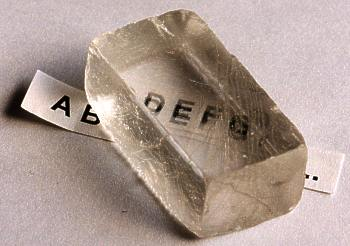
\includegraphics{images/calcit.jpg}
\caption{Kalkspat (Calcit) kann also Analysator f"ur die Polarisation
von Photonen dienen. Er zerlegt einen Strahl von Photonen in zwei
Strahlen mit orthogonaler Polarisierung.
\label{calcit}}
\end{figure}
\index{Kalkspat}
\index{Calcit}
\index{Doppelbrechung}
Kalkspat (Calcit) (Abbildung~\ref{calcit}) teilt einen Strahl
von Photonen auf in zwei Strahlen mit orthogonaler Polarisierung,
funktioniert also als Analysator f"ur zwei Polarisationsrichtungen
von Photonen.

\index{Analysatorkreis}
Man kann sich auch vorstellen, die vom Analysator getrennten Strahlen
wieder zusammenzuf"uhren, schematisch:
\begin{center}
\includegraphics{graphics/analysator-2.pdf}
\end{center}
Wir nennen ein solches Objekt einen {\em Analysatorkreis}, auch wenn wie
im n"achsten Beispiel nicht alle Pfade wieder zum Ausgang zusammengef"ugt
werden.

Wir k"onnen vor dem Zusammenf"ugen der Strahlen einzelne davon
blockieren, z.~B.~$a_2$:
\begin{center}
\includegraphics{graphics/analysator-3.pdf}
\end{center}
\index{Projektor}
Wir nennen diese Schaltung auch einen {\em Projektor}, er reduziert den
urspr"unglichen Strahl auf einen Zustand, dem die Komponenten $a_2$
fehlt. Nat"urlich k"onnen Projektoren f"ur eine beliebige Teilmenge
$A=\{a_{i_1},\dots, a_{i_k}\}$ definiert werden: der Projektor $P_A$
blokiert genau die Komponenten aus der Menge $A$.
\index{idempotent}
Damit die oben gezeigten Schemata f"ur Analysatoren ihre G"ultigkeit
haben, sollten Projektoren {\em idempotent}, d.~h.~zwei identische 
Projektoren wirken genau gleich wie ein einzelner, also $P^2=P$ oder
schematisch:
\begin{center}
\includegraphics{graphics/analysator-4.pdf}
\end{center}

Dies ist nur m"oglich, wenn die Wahscheinlichkeit, ein Teilchen nach
einem Projektor $P_{\{a_i\}}$ im Zustand $a_i$ zu finden, verschwindet.
Jeder andere Zustand muss hingegen unver"andert durchkommen, also
\[
P(a_i|a_j)=\delta_{ij}=\begin{cases}
1&\qquad i\ne j\\
0&\qquad\text{sonst.}
\end{cases}
\]
Ein solcher Satz von Zust"anden nennen wir eine Basis.

Nat"urlich sollen die Zust"ande alle m"oglichen Situationen abdecken
k"onnen, es sollte also keinen Zustand $|\psi\rangle$ geben, so dass
\[
P(a_i|\psi)=0\quad\forall i.
\]

\index{Observable}
In der Quantenmechanik sind also genau jene Gr"ossen messbar, f"ur die
es einen Analysator gibt, man nennt solche Gr"ossen {\em Observable}.
Die Polarisierung von Photonen, die Position oder der Impuls
eines Teilchens, das elektrische Dipolmoment eines Atoms sind alle
Observable.

\subsection{Photonenpolarisierung}
Betrachten wir als Beispiel Photonen und ihre Polarisation. 
Statt einer Basis aus den Zust"anden, die horizontal ($a_1$) und vertikal
($a_2$) polarisierte Photonen beschreiben, k"onnen wir auch zwei 
beliebige andere Polarisationsrichtungen $b_1$ und $b_2$ verwenden,
oder sogar rechts ($c_R$) und links ($c_L$) zirkul"ar polarisierte Photonen.
Seien also $b_1$ und $b_2$ gegen"uber $a_1$ und $a_2$ um den Winkel
$\alpha$ verdreht, dann wird die Intensit"at eines Strahls aus $a_2$
bei der Analyse mit $b_1$ und $b_2$ folgende Werte ergeben:
\begin{equation}
\begin{aligned}
P(b_1|a_2)&=\sin^2\alpha
&\qquad
P(b_2|a_2)&=\cos^2\alpha
\\
P(b_1|a_1)&=\cos^2\alpha
&
P(b_2|a_1)&=\sin^2\alpha.
\end{aligned}
\label{polarisation-projektion}
\end{equation}
Die Wahrscheinlichkeiten sind proportional zu den Intensit"aten,
die proportional zum Quadrat der Amplituden sind (daher die Quadrate
in (\ref{polarisation-projektion}).
\begin{figure}
\centering
\includegraphics{graphics/analysator-5.pdf}
\caption{Projektion des Zustandes $|a_2\rangle$ auf die beiden
um $\alpha$ verdrehten Basiszust"ande $|b_1\rangle$ und $|b_2\rangle$.
\label{polarisation-rotation}}
\end{figure}
Man beachte, dass sich aus der Abbildung auch ableiten l"asst, dass
\begin{equation}
\begin{aligned}
P(a_1|b_1)&=\cos^2\alpha
&\qquad
P(a_1|b_2)&=\sin^2\alpha
\\
P(a_2|b_1)&=\sin^2\alpha
&
P(a_2|b_2)&=\cos^2\alpha.
\end{aligned}
\label{polarisation-projektion-inverse}
\end{equation}
\index{Ubergangswahrscheinlichkeit@\"Ubergangswahrscheinlichkeit}
Man beachte, dass die "Ubergangswahrscheinlichkeiten
symmetrisch sind: $P(a_i|b_j)=P(b_j|a_i)$.
Ausserdem ergeben die Elemente $P(a_i|b_j), 1\le i\le n$ f"ur festes $j$,
zusammen den Wert $1$:
\[
\sum_{i=1}^nP(a_i|b_j)=1\quad\forall j.
\]
F"ur zirkul"ar polarisierte Photonen gilt immer 
\[
P(z_L|a_i)=P(z_R|a_i)=\frac12.
\]
Das Experiment in Abbildung~\ref{linear-zirulaer} 
\begin{figure}
\centering
\includegraphics{graphics/analysator-6.pdf}
\caption{Experiment zur Messung des Zusammenhanges zwischen zirkul"arer
und linearer Polarisierung. Der rot hervorgehobene Block wird sp"ater
zur Berechnung von $P(c_L|a_2)$ verwendet.
\label{linear-zirkulaer}}
\end{figure}
An der Stelle~1 ist der Strahl in Richtung $a_2$ linear polarisiert.
An der Stelle~2 ist er links-zirkul"ar polarisiert. Die Wahrscheinlichkeit,
das Intensit"atsverh"altnis der Strahlen zwischen den Punkten $1$ und $2$
ist
\begin{equation}
\frac{I_2}{I_1}=P(c_L|a_2)=\frac12.
\label{intensitaetsverhaeltnis}
\end{equation}

\subsection{Doppelspaltexperiment}
\index{Doppelspaltexperiment}
\begin{figure}
\centering
\includegraphics{graphics/analysator-7.pdf}
\caption{Doppelspaltexperiment Teilchen mit gleichem Impuls oder Photonen
mit gleicher Wellenl"ange treffen von rechts auf eine Blende mit zwei
Spalten. Auf dem Schirm links werden die Teilchen gez"ahlt, die dort
eintreffen. Es entsteht ein Interferenzmuster.
\label{doppelspalt-bild}}
\end{figure}
Das ber"uhmte Doppelspaltexperiment (Abbildung~\ref{doppelspalt-bild})
erzeugt zun"achst einen Strahl
von Teilchen, die alle den gleichen Impuls $p$ haben, wir haben also
Teilchen im Zustand $|p\rangle$. Dieser Strahl
wird dann auf die zwei Spalte gerichtet. Dadurch wird der Strahl
beeinflusst, es entsteht also ein neuer Zustand, den zu berechnen
wir uns f"ur sp"ater zur Aufgabe machen wollen.
Im Moment bezeichnen wir diesen Zustand nach dem Doppelspalt 
als $|\psi\rangle$.

Gemessen wird dann, mit welcher Wahrscheinlichkeit
ein Teilchen im Zustand mit Position $y$ auf dem Schirm
gemessen wird, wenn das Teilchen im Zustands $|\psi\rangle$
ist. Dies ist ein bedingte Wahrscheinlichkeit, die wir also
$P(y|\psi)$ geschrieben werden kann.

Wir k"onnen dieses Experiment auch mit dem bisher entwickelten
Formalismus analysieren.
Zun"achst k"onnen wir die Blende als einen Analysator auffassen, der
den Strahl aufspaltet in verschiedene Zust"ande von Teilchen, die
den einen oder anderen Spalt traversiert haben.
Die Zust"ande $B_1$, $B_2$ und $B_3$ entsprechen Teilchen, die die
Blende nicht passiert haben. Die Zust"ande $S_1$ und $S_2$ entsprechen
Teilchen, die durch die beiden Spalte $S_1$ und $S_2$ geflogen sind.

Die unendlich vielen m"oglichen Positionen $y$ auf dem Schirm
k"onnen wir ebenfalls auf diskrete Zust"ande abbilden.
Dazu unterteilen wir den Schirm links in
disjunkte Zonen, die das Eintreffen eines Teilchens registrieren k"onnen.
Ein Teilchen kann offenbar nur in jeweils einer Zone registriert werden.
Bezeichnen wir die den Zustand eines Teilchens, welches in der Zone mit
der Nummer $i$ registriert wird, mit $y_i$, dann funkioniert der Schirm als
eine Kombination von Projektoren auf die Zust"ande $|y_i\rangle$.
\begin{figure}
\centering
\includegraphics{graphics/analysator-8.pdf}
\caption{Analyse des Doppelspalt-Experiments
\label{doppelspalt-analyse}}
\end{figure}
Das kombinierte Experiment sieht dann aus wie in
Abbildung~\ref{doppelspalt-analyse}

\section{Algebraischer Formalismus der Quantenmechanik}
\rhead{Algebraischer Formalismus}
Im letzten Abschnitte haben wir einige Prinzipien zusammengestellt,
die ein quantenmechanischer Kalk"ul wiederzugeben in der Lage sein muss.
Wir brauchen nur noch eine algebraische Struktur, mit der wir die 
verschiedenen Objekte abbilden k"onnen.

\subsection{Analysatoren}
\index{Analysator}
Eine ununterbrochene Kurve in einem Analysatorkreis durch den Zustand
$a_i$ stellen wir durch das ``Messsymbol'' 
\[
|a_i\rangle\langle a_i|
\]
dar. Das Symbol ist von rechts zu lesen: wenn ein Teilchen
im Zustand $a_i$ auf den Analysator trifft, dann gibt er ein solches
Teilchen weiter.

Ein Analysatorkreis, der am Input nichts "andert, entspricht dem Symbol
\[
\sum_{i=1}^n |a_i\rangle \langle a_i|=\operatorname{id},
\]
dieses Objekt wirkt wie die identische Abbildung.
\index{Abbildung!identische}

\subsection{Projektoren}
\index{Projektor}
Ein einzelner Projektor auf einen Basiszustand $a_i$ entspricht dem Symbol
$P= |a_i\rangle\langle a_i|$, also muss gelten
\[
P^2 = 
|a_i\rangle\langle a_i|
\cdot
|a_i\rangle\langle a_i|
=P
=
|a_i\rangle\langle a_i|.
\]
Zwei verschiedene Projektoren m"ussen sich hingegen aufheben:
\[
|a_i\rangle\langle a_i|
\cdot
|a_j\rangle\langle a_j|
=
0 \quad\text{f"ur $i\ne j$}.
\]
Man kann also schreiben
\[
|a_i\rangle\langle a_i|
\cdot
|a_j\rangle\langle a_j|
=\delta_{ij} |a_i\rangle\langle a_j|.
\]
Ein allgemeiner Projektor $P$, der nur die Zust"ande $a_{i_1},\dots ,a_{i_m}$
akzeptiert, wird als
\[
P = \sum_{k=1}^m |a_{i_k}\rangle \langle a_{i_k}|
\]
geschrieben.
Nach den eben abgeleiteten Rechenregeln gilt
\begin{align*}
P^2
&=
\sum_{k,l=1}^m |a_{i_k}\rangle\langle a_{i_k}|a_{i_l}\rangle\langle a_{i_l}|
=
\sum_{k,l=1}^m \delta_{i_ki_l}|a_{i_k}\rangle\langle a_{i_l}|
=
\sum_{k=1}^m |a_{i_k}\rangle\langle a_{i_k}| = P
\end{align*}
$P$ ist also tats"achlich ein Projektor.

Diese Beobachtungen sind konsistent mit der Annahme, dass
\[
\langle a_i|a_j\rangle = \delta_{ij}.
\]

\subsection{Transformationsfunktion}
\index{Transformationsfunktion}
Bisher wurden nur Messsymbole miteinander verkn"upft, deren 
Verkn"upfung bereits bekannt war, es stellt sich daher die
Frage gar nicht, was das naheliegende Symbol $\langle B|C\rangle$
in
\[
|A\rangle\langle B|\cdot |C\rangle\langle D|
=
|A\rangle \langle B|C\rangle \langle D|
\]
f"ur eine Bedeutung haben soll. Die bisherigen Beispiel konnte
man so interpretieren, dass $\langle B|C\rangle$ eine Zahl war
(in den Beispielen jeweils $0$ oder $1$).
Eine naheliegende Verallgemeinerung ist daher, immer anzunehmen,
dass $\langle B|C\rangle$ eine Zahl ist, und dass man mit den
Messsymbolen wie f"ur Matrizen "ublich rechnen kann.
Es kommt also auf die Reihenfolge der Faktoren an, aber skalare
Faktoren, wie eben auch $\langle B|C\rangle$ k"onnen beliebig
verschoben werden.
$\langle \,\cdot\, |\,\cdot\, \rangle$ heisst die Transformationsfunktion.

%Die Transformationsfunktion taucht auf als Koeffizient in Linearkombinationen
%von Messsymbolen.

Wenden wir den eben entwickelten Formalismus auf das Doppelspalt-Experiment
gem"ass Abbildung~\ref{doppelspalt-analyse} an, erhalten wir das Symbol
\[
|y_i\rangle \langle y_i|\; (|S_1\rangle\langle S_1| + |S_2\rangle \langle S_2|)
=
\langle y_i|S_1\rangle
\cdot
|y_i\rangle \langle S_1|
+
\langle y_i|S_2\rangle
\cdot
|y_i\rangle \langle S_2|,
\]
\index{Uberlagerung@\"Uberlagerung}
Insbesondere entsteht die Intensit"at in der Zonen $y_i$ durch eine
"Uberlagerung von zwei Termen mit verschiedenen
Koeffizienten $\langle y_i|S_j\rangle, j=1,2$.
\index{Interferenz}
Das Resultat der Durchf"uhrung des Experiments zeigt ein Interferenz-Muster,
was alleine mit reellen Werten f"ur die Transformationsfunktion nicht
zu bewerkstelligen w"are.
Wir m"ussen daher davon ausgehen, dass $\langle B|C\rangle\in\mathbb C$ gilt.

Mit Hilfe der Transformationsfunktion kann mit Hilfe einer Basis von Zust"anden
$|a_i\rangle, i=1,\dots, n,$ und einem Zustand $|\psi\rangle$ einen Vektor
\[
\begin{pmatrix}
\langle a_1|\psi\rangle\\
\vdots\\
\langle a_n|\psi\rangle
\end{pmatrix}
\in\mathbb C^n
\]
zuordnen.
Eine Basis transportiert eine Problem "uber Zust"ande in ein
Problem "uber Vektoren in $\mathbb C^n$.

\subsection{Wahrscheinlichkeiten}
\index{Wahrscheinlichkeit}
Zu dem Experiment in Abbildung~\ref{linear-zirkulaer} geh"ort das Symbol
\[
|a_2\rangle\langle a_2|\cdot
|c_L\rangle\langle c_L|\cdot
|a_2\rangle\langle a_2|
=
|a_2\rangle\langle a_2
|c_L\rangle\langle c_L
|a_2\rangle\langle a_2|
=
\langle a_2
|c_L\rangle\langle c_L
|a_2\rangle
|a_2\rangle
\langle a_2|
\]
Andererseits haben wir das Intensit"atsverh"altnis zwischen den Punkten
$1$ und $2$ bereits in (\ref{intensitaetsverhaeltnis}) ausgerechnet.
Der rot eingerahmte Teil des Experimentes scheint dem Ausdruck
\[
\langle a_2
|c_L\rangle\langle c_L
|a_2\rangle
\]
zu entsprechen.
Dies suggeriert, dass wir ihn als
\[
\langle a_2
|c_L\rangle\langle c_L
|a_2\rangle
=
P(c_L|a_2) 
\]
interpretieren k"onnten. F"ur diesen Ausdruck ist die fr"uher formulierte
Symmetriebedingung 
\[
P(A|B)
=
\langle A |B\rangle
\langle B |A\rangle
=
\langle B |A\rangle
\langle A |B\rangle
=
P(B|A)
\]
ebenfalls erf"ullt.

Da $P(A|A) =1$ ist, folgt
\begin{align*}
P(A|A)&=\langle A|A\rangle \langle A|A\rangle = \langle A|A\rangle = 1
\\
\langle A|A\rangle&=\pm 1
\end{align*}
Der negative Wert ist nicht weiter n"utzlich, so dass wir im folgenden
davon ausgehen, dass $\langle A|A\rangle = 1$ gilt.

Die Wahrscheinlichkeit $P(A|B)$ muss $\ge 0$ sein, also insbesondere
reell. Das ist nur dann garantiert, wenn $\langle A|B\rangle$ und
$\langle B|A\rangle$ konjugiert komplex sind:
\begin{equation}
\langle B|A\rangle
=\overline{\langle A|B\rangle}.
\label{hermiteschesymmetrie}
\end{equation}
Wir nennen dies die {\em hermitesche} Symmetrie der Transformationsfunktion.

\subsection{Observable und Operatoren}
\index{Observable}
Bisher haben wir nur Analysatoren und Projektoren untersucht.
Es ist aber durchaus denkbar, dass noch wesentlich komplexere
Versuchsaufbauten existieren, deren Details wir gar nicht unbedingt
im Detail kennen:
\begin{center}
\includegraphics{graphics/analysator-9.pdf}
\end{center}
Ist eine Basis $|a_i\rangle$ von Zust"anden gegeben, dann k"onnen
wir die Wirkung von $A$ auf die Wirkung auf den Zustandsvektoren
reduzieren, indem wir $A$ mit Analysatorkreisen zusammensetzen:
\begin{center}
\includegraphics{graphics/analysator-10.pdf}
\end{center}
Diesem Diagramm entspricht der Ausdruck
\[
|a_j\rangle \langle a_j|\, A \,|a_i\rangle \langle a_i|,
\]
insbesondere ist die Wirkung von $A$ vollst"andig festgelegt durch die
Zahlen
$\langle a_j|A|a_i\rangle$, sie heissen die {\em Matrixelemente} von $A$.
\index{Matrixelement}
Die Wirkung von $A$ auf dem Zustand $|\psi\rangle$ ist also
\begin{equation}
A|\psi\rangle = \sum_{i,j} |a_j\rangle
	\langle a_j|\,A\,|a_i\rangle
	\langle a_i|\psi\rangle,
\label{A-wirkung}
\end{equation}
mit Hilfe einer Basis kann man also die Wirkung eines Operators auf
die Multiplikation von Matrizen und Vektoren
\[
\begin{pmatrix}
\langle a_1|\,A\,|\psi\rangle\\
\vdots\\
\langle a_n|\,A\,|\psi\rangle
\end{pmatrix}
=
\begin{pmatrix}
\langle a_1|\,A\,|a_1\rangle&\dots &\langle a_1|\,A\,|a_n\rangle\\
\vdots                  &\ddots&\vdots                  \\
\langle a_n|\,A\,|a_1\rangle&\dots &\langle a_n|\,A\,|a_n\rangle
\end{pmatrix}
\begin{pmatrix}
\langle a_1|\psi\rangle\\
\vdots\\
\langle a_n|\psi\rangle
\end{pmatrix}
\]
reduzieren.

In (\ref{A-wirkung}) wurde angenommen, dass $A$ auf den Vektor
$|\psi\rangle$ wirkt. Die Notation ist jedoch symmetrisch, k"onnte
man auch eine Wirkung von $A$ auf Vektoren $\langle\psi|$ entwickeln?
Diese Wirkung schreiben wir
\[
A\langle \psi|=\langle\psi|A^*.
\]
Mit Hilfe der hermiteschen Symmetrierelation (\ref{hermiteschesymmetrie})
kann man aber auch die Wirkung auf einen $\langle\psi|$-Vektor ausrechnen:
\begin{equation}
(A\langle a_i|)\,|a_j\rangle
=
\overline{\langle a_j|\,(A\,|a_i\rangle)}
=
\overline{\langle a_j|\,A\,|a_i\rangle}.
\end{equation}
Die Matrix von $A^*$
ist also die transponierte und komplex konjugierte Matrix von $A$,
sie heisst auch die {\em adjungierte} Matrix.
\index{adjungierte Matrix}

Operatoren sind beliebige Linearkombinationen von Messsymbolen,
F"ur Projektoren waren es ausschliesslich Messsymbole der Form
$|a_i\rangle\langle a_i|$, ein komplexer Operator $A$ kann jedes
Messymbol enthalten, die Matrixelemente sind die Koeffizienten 
der Linearkombination.

Damit k"onnen wir jetzt auch eine algebraische Definition einer
Observablen geben. Observable sind Gr"ossen, f"ur die es einen
Analysator gibt. Insbesondere gibt es eine Basis von Zust"anden,
die zu verschiedenen Werten der Observablen geh"oren.
Seien $|i\rangle$ die Zust"ande, und $v_i$ die Werte der Observablen
f"ur den Zustand $|i\rangle$. Dann k"onnen wir einen neuen
Operator
\[
V = \sum_{i} a_i\, |i\rangle\langle i|
\]
bauen. In der Basis $|i\rangle$ sind die Matrixelement von $V$
\[
\langle j|\,V\,|i\rangle = v_i\delta_{ij},
\]
$V$ hat also Diagonalform. In einer anderen Basis muss dies nicht
mehr erf"ullt sein. Es ist aber eine entscheidende Eigenschaft 
von $V$, dass es eine Basis gibt, in der $V$ diagonal wird.

Ist $|\psi\rangle$ ein beliebiger Zustand, dann ist
\[
\langle\psi|V|\psi\rangle
=
\sum_{i,j}\langle \psi|j\rangle\langle j|\,V\,|i\rangle\langle i|\psi\rangle
=
\sum_i\langle \psi|i\rangle\langle i|\,V\,|i\rangle\langle i|\psi\rangle
=
\sum_i v_i P(i|\psi)=E(V|\psi),
\]
also ist $\langle \psi|V|\psi\rangle$ der Erwartungswert der Observablen
$V$ im Zustand $\psi$.

% XXX Definition von selbstadjungiert...
\index{selbstadjungiert}
Allgemein betrachten wir selbstadjungierte Operatoren also 
die Repr"asentanten von Observablen, denn aus der abstrakten
Theorie der komplexen Vektorr"aume ist bekannt, dass selbstadjungierte
Matrizen diagonalisierbar sind.

\subsection{Zusammenfassungen}
Wir fassen den bisher entwickelten Formalismus zusammen.

\begin{enumerate}
\item
In der Quantenmechanik werden Zust"ande durch Vektoren $|\psi\rangle$
eines noch nicht spezifizierten Vektorraumes dargestellt.
\item
Zu jedem Vektor $|\phi\rangle$ gibt es auch einen Vektor $\langle \phi|$,
sowie die Paarungen
$|\phi\rangle\langle\psi|$
und
$\langle\phi|\psi\rangle$.
$|\phi\rangle\langle\psi|$ heisst das Messsymbol, es akzeptiert Teilchen im
Zustand $|\psi\rangle$ und wandelt sie in solche im Zustand $|\phi\rangle$
um.
\item
Die Gr"osse $\langle \phi|\psi\rangle$ ist eine komplexe Zahl, sie
heisst die Transformationsfunktion. Es gilt
\begin{align*}
\langle \phi|\psi\rangle
&=
\overline{
\langle \psi|\phi\rangle
}
\\
\langle\psi|\psi\rangle&=1
\end{align*}
Die physikalische Bedeutung von $\langle\phi|\psi\rangle$ ist die
Wahrscheinlichkeit
\[
P(\phi|\psi)=|\langle \phi|\psi\rangle|^2=
\langle\phi|\psi\rangle
\langle\psi|\phi\rangle,
\]
in einem Strahl von Teilchen im Zustand $|\psi\rangle$ ein Teilchen zu
finden, welches sich im Zustand $|\phi\rangle$ befindet.
\item Kann ein Zielzustand auf "uber verschiedene Zwischenzust"ande
erreicht werden, dann ist die Transformationsfunktion die Summe
der Transformationsfunktionen f"ur die Zwischenzust"ande:
\[
\langle A|B\rangle
=
\sum_{i=1}^n\langle A|b_i\rangle\;\langle b_i|B\rangle.
\]
\item
Besteht ein Weg aus mehreren Schritten, dann ist ihre Transformationsfunktion
das Produkt der Transformationsfunktionen der einzelnen Schritte.
\item 
Observable sind selbstadjungierte Operatoren.
Bilden die Zust"ande $|i\rangle$ eine Basis, in der die Observable $A$ 
diagonal ist, dann ist das Matrix-Element $\langle i|A|i\rangle$ der
Wert der Observablen im Zustand $|i\rangle$. F"ur einen beliebigen
Zustand $|\psi\rangle$ ist $\langle\psi|V|\psi\rangle$ der Erwartungswert
der Observablen $V$ im Zustand $|\psi\rangle$.
\end{enumerate}

%
% Zeitentwicklung
%
\section{Zeitentwicklung}
\rhead{Zeitentwicklung}
\index{Zeitentwicklung}
Die besondere Erkenntnis Newtons war, dass die Gleichung $F=ma$ eine
Differentialgleichung ist, die zusammen mit einer Anfangsbedingung die
gesammte zuk"unftige Bewegung festlegt.
Wir m"ochten ein "ahnlich leistungsf"ahiges Prinzip auch in der
Quantenmechanik haben.
Getreu mit dem bisher entwickelten Formalismus k"onnen wir bestenfalls
erwarten, eine Differentialgleichung f"ur die Entwicklung des Zustandes
zu finden, also zum Beispiel
\begin{equation}
\frac{d}{dt}|\psi(t)\rangle = F(t, |\psi(t)\rangle)
\label{zeitentwicklung}
\end{equation}
f"ur eine m"oglicherweise komplizierte Funktion $F$.

Die Quantenmechanik ist also immer noch vollst"andig {\em deterministisch},
zu einem gegebenen Anfangszustand geh"oren eindeutig bestimmte
zuk"unftige Zust"ande.
Die Schwierigkeit kann aber darin bestehen, dass der Anfangszustand nicht
unbedingt bekannt ist.
Wir werden zum Beispiel sehen, dass wir die Position eines Teilchens
nicht wirklich kennen k"onnen, man kann ein Teilchen nicht in
einen Zustand bringen, wo die Position mit beliebiger Genauigkeit
bekannt ist.
Ausserdem k"onnen wir aus der Zeitentwicklung nicht beliebige Aussagen
ableiten, sondern nur Informationen die sich aus $|\psi(t)\rangle$ 
mit Hilfe von Observablen errechnen lassen,
Dies sind aber ausschliesslich Erwartungswerte der Observablen oder
Wahrscheinlichkeiten f"ur einzelne Werte.
Die Quantenmechanik kann nicht vorhersagen, welchen Wert f"ur eine
bestimmte Observable wir in einem Experiment messen werden.
Quantenmechanische Vorhersagen sind also immer von statistischer Art.


Die Funktion $F$ ist nicht beliebig, es muss ja zum Beispiel zu allen Zeiten
gelten
$\langle\psi(t)|\psi(t)\rangle=1$, was die Wahl der Funktion $F$ einschr"ankt.
In unserem Formalismus kann die Zeitentwicklung als abstrakter Block
gezeichnet werden:
\begin{center}
\includegraphics{graphics/analysator-11.pdf}
\end{center}
Wir erwarten daher, dass die Zeitentwicklung wieder ein Operator ist,
den wir $U(t)$ nennen:
\[
|\psi(t)\rangle = U(t)\,|\psi(0)\rangle.
\]
Das bedeutet aber, dass die Differentialgleichung (\ref{zeitentwicklung})
linear sein muss, es muss also einen m"oglicherweise zeitabh"angigen
Operator $K(t)$ geben, so dass 
\begin{equation}
\frac{d}{dt}\,|\psi(t)\rangle = K(t)\,|\psi(t)\rangle.
\label{zeitentwicklung-linear}
\end{equation}
Die L"osung dieser Differentialgleichung liefert den Operator $U(t)$,
wobei $U(0)$ die identische Abbildung (Einheitsmatrix) sein muss.

Zun"achst m"ussen wir sicherstellen, dass $\langle\psi(t)|\psi(t)\rangle=1$
f"ur alle Zeiten. Dies ist offenbar eine Aussage "uber den Operator $U(t)$,
den wir in diesem Absatz einfach als $U$ schreiben.
Zu jedem beliebigen Anfangszustand $|\psi(0)\rangle$ muss gelten
\[
\langle \psi(t)|\psi(t)\rangle
=
\langle \psi(t)|\,U\,|\psi(0)\rangle
=
\overline{\langle\psi(0)|\,U^*\,|\psi(t)\rangle}
=
\overline{\langle\psi(0)|\,U^*U\,|\psi(0)\rangle}
=
\langle\psi(0)|\,U^*U\,|\psi(0)\rangle.
\]
Dies ist nur m"oglich, wenn
\begin{equation}
U^*U=\operatorname{id}
\label{unitaritaetsbedingung}
\end{equation}
die identische Abbildung ist. Der Operator $U(t)$ muss also unit"ar sein.
\index{unitar@unit\"ar}

Die Unitarit"at von $t$ schr"ankt $K(t)$ stark ein. Leiten wir die
Unitarit"atsbedinung (\ref{unitaritaetsbedingung}) nach der Zeit ab,
und werten die Ableitung an der Stelle $t=0$ aus,
erhalten wir die Gleichung
\[
0
=
\left.\frac{d}{dt}\bigl(U(t)^*U(t)\bigr)\right|_{t=0}
=
\left.
\biggl(
\frac{dU(t)^*}{dt}U(t)+U(t)^*\frac{dU(t)}{dt}
\biggr)
\right|_{t=0}
=
\biggl(\frac{dU(0)}{dt}\biggr)^*
+
\biggl(\frac{dU(0)}{dt}\biggr).
\]
Schreiben wir $K$ f"ur die Ableitung von $U(t)$ an der Stelle $t=0$,
dann muss offenbar gelten
\[
K^*+K=0\qquad\Rightarrow\qquad K^*=-K,
\]
man sagt auch, $K$ sei {\em antihermitesch}. Aus $K$ kann man einen
neuen Operator
\[
H=-\frac{\hbar}{i}K=i\hbar K
\]
konstruieren, f"ur den gilt
\[
H^*
=
\left(-\frac{\hbar}{i}K\right)^*
=
+\frac{\hbar}{i}K^*
=
-\frac{\hbar}{i}K=H.
\]
Insbesondere ist $H$ ein selbstadjungierter Operator, oder
eine Observable.
\index{Hamilton-Operator}
Der Faktor $\hbar$ wird konventionell verwendet, es wird sich
herausstellen, dass sich damit $H$ einfacher mit einer bekannten
physikalischen Gr"osse identifizieren l"asst.
Die Masseinheit von $H$ ist die Masseinheit von $\hbar$ geteilt durch die Zeit.
Da $\hbar$ die Masseinheit $\text{J}\cdot\text{s}$ hat, hat
$H$ die Masseinheit einer Energie.
Nat"urlich ist das keine Begr"undung f"ur irgend etwas, denn die
Masseinheit entstand ja durch die Wahl des Faktors $\hbar$, f"ur
welche wir noch gar keine Begr"undung haben.

Die Differentialgleichung f"ur die Zeitentwicklung des Quantensystems wird
mit $H$ ausgedr"uckt zu
\begin{equation}
i\hbar\frac{d}{dt}|\psi(t)\rangle = H(t)\,|\psi(t)\rangle,
\label{schroedingergleichungt}
\end{equation}
die {\rm zeitabh"angige Schr"odingergleichung}.
\index{schrodingergleichung@Schr\"odingergleichung!zeitabh\"angige}

Falls $H$ nicht von der Zeit abh"angt, wird die zeitabh"angige zur
zeitunabh"angigen Schr"odingergleichung
\index{schrodingergleichung@Schr\"odingergleichung!zeitunabh\"angige}
\begin{equation}
i\hbar \frac{d}{dt}\,|\psi(t)\rangle = H\,|\psi(t)\rangle,
\label{schroedingergleichung}
\end{equation}
die mit Hilfe der Exponentialfunktion sofort gel"ost werden kann:
\[
|\psi(t)\rangle = e^{i\hbar H}\,|\psi(0)\rangle
\]
Da $H$ eine Observable ist, k"onnen wir eine Basis von Eigenvektoren
von $H$ konstruieren, ist $|k\rangle$ ein Eigenvektor von $H$ mit
Eigenwert $E_k$, dann ist die Zeitentwicklung f"ur $|\psi(0)\rangle = |k\rangle$
\[
|\psi(t)\rangle
=
e^{i\hbar E_k}\,|k\rangle.
\]
Insbesondere ist in diesem Spezialfall eines zeitunabh"angigen $H$-Operators
die Zeitentwicklung vollst"andig bekannt, wenn man die Eigenwerte und
Eigenvektoren von $H$ bestimmt hat.

%
% Zeitentwicklung von Observablen
%
\subsection{Zeitentwicklung von Observablen}
\index{Zeitentwicklung!von Observablen}
Sei $|\psi(t)\rangle$ ein Zustand, der die zeitunabh"angige
Schr"odingergleichung mit Hamilton-Operator $H$ erf"ullt. Wir m"ochten
gerne wissen, wie sich die Observable $A$ mit der Zeit entwickelt,
wie gross also
\begin{equation}
\langle A\rangle
=
\langle \psi(t)|A|\psi(t)\rangle
\label{observable-zeitabhaengigkeit}
\end{equation}
sein wird. Dazu leiten wir (\ref{observable-zeitabhaengigkeit}) nach der
Zeit ab und setzen die Schr"odingergleichung ein:
\begin{align*}
\frac{d}{dt}\langle A\rangle
&=
\biggl(\frac{d}{dt}\langle\psi(t)|\biggr)A\,|\psi(t)\rangle
+
\langle\psi(t)|\,A\biggl(\frac{d}{dt}\,|\psi(t)\rangle\biggr)
\\
&=
\biggl(\frac{1}{i\hbar}H\langle\psi(t)|\biggr)A\,|\psi(t)\rangle
+
\langle\psi(t)|\,A\frac{1}{i\hbar}H\,|\psi(t)\rangle
\\
&=
\frac{i}{\hbar}
\langle\psi(t)|\, HA-AH \,|\psi(t)\rangle
\\
&=\langle\psi(t)|\, \frac{i}{\hbar}[H,A] \,|\psi(t)\rangle
\end{align*}
Die Zeitabh"angigkeit einer Observablen $A$ wird also im Wesentlichen
durch den Kommutator $[H,A]$ der Observablen mit dem Hamiltonoperator $H$
gegeben. Erhaltungsgr"ossen sind also solche Observable, die mit dem
Hamiltonoperator vertauschen.




\chapter{Hilbertr"aume}
\lhead{Hilbertr"aume}
\rhead{}
Wir wissen schon, dass Zust"ande Eigenvektoren des Hamilton-Operators
sein sollen, wir brauchen
also einen Vektorraum, der ausreichend gross ist, alle Zust"ande aufzunehmen.
Ein typisches Quantensystem hat eine sehr grosse Zahl von Zust"anden,
vielleicht sogar unendlich viele.
Wir brauchen daher einen unendlichdimensionalen komplexen Vektorraum als
B"uhne f"ur die Quantenmechanik.
Der Begriff des Hilbertraumes liefert die gesuchte Struktur.

Ausgehend von der gewohnten Vorstellung eines endlichdimensionalen
Vektorraumes kann in vier Schritten eine ausreichend reichhaltige
Struktur aufgebaut werden:
\begin{enumerate}
\item Erweiterung der Definition eines reellen Vektorraumes dahingehend,
dass auch komplexe Skalare zugelassen werden.
\item Erweiterung des Begriffs des Skalarprodukts auf den komplexen Fall.
Dazu geh"oren auch der Begriff der L"ange eines Vektors und Ungleichungen
wie die Dreiecksungleichung, die unsere Intuition f"ur das Verhalten von
Abst"anden auf den unendlichdimensionalen Fall erweitern.
\item Der Begriff des Grenzwertes einer Vektorfolge erlaubt, Zust"ande
zu approximieren.
\item Die Hilbertbasis liefert eine Technik, wie die Zust"ande eines
Quantensystems als Basisvektoren f"ur den Zustandsraum verwendet werden
k"onnen.
\end{enumerate}

\section{Komplexe Vektorr"aume}
Ein Vektorraum "uber $\mathbb C$ ist einem Menge $V$ von Vektoren, mit
einer Addition von Vektoren und einer Multiplikation von Vektoren mit
komplexen Zahlen, mit folgenden Eigenschaften
\begin{compactenum}
\item Es gibt ein Element $0\in V$ mit der Eigenschaft $0+v=v,\forall v\in V$
und $0v=0$.
\item Zu jedem $v\in V$ gibt es ein Elemente $-v=(-1)v$ mit der Eigenschaft
$v+(-v)=0$
\item $u+v=v+u$
\item $(u+v)+w=u+(v+w)$
\item $(\lambda\mu)v=\lambda (\mu v)$
\item $\lambda(u+v)=\lambda u+ \lambda v$, $\lambda\in\mathbb C$, $u,v\in V$
\item $(\lambda+\mu)u=\lambda u+\mu u$
\end{compactenum}
Wie im Falle reeller Vektorr"aume kann man den Vektorraum
\[
{\mathbb C}^n = \left\{\left .
\begin{pmatrix}x_1\\\vdots\\x_n\end{pmatrix}
\right|
x_i\in\mathbb C
\right\}
\]
mit komponentenweisen Operationen konstruieren.
Ebenso kann man lineare Gleichungssysteme mit komplexen Koeffizienten,
komplexe Matrizen und das Matrizenprodukt f"ur komplexe Matrizenprodukt
konstruieren.

Der Gauss-Algorithmus kann unver"andert auch f"ur komplexe Gleichungssysteme
verwendet werden, so dass alle Eigenschaften, die man mit Hilfe des
Gauss-Algorithmus hergeleitet hat, auch f"ur komplexe Vektorr"aume
gelten.
Insbesondere ist der Rang definiert, die L"osungsmenge
eines Gleichungssystems ist eine Menge von komplexen Linearkombinationen
von Vektoren, und die (komplexe) Determinate ist genau dann 0, wenn
die Matrix singul"ar ist.

\section{Komplexes Skalarprodukt}
Das Skalarprodukt in reellen Vektorr"aumen ist eine Funktion von
zwei Vektoren, die linear ist in jedem Faktor:
\begin{align*}
(a+b,c)&=(a,c)+(b,c)&(a,b+c)&=(a,b)+(a,c)\\
(\lambda a,b)&=\lambda(a,b)&(a,\lambda b)&=\lambda(a,b)
\end{align*}
W"urde man diese Definition f"ur komplexe Zahlen verwenden, dann
m"usste das Skalarprodukt eines komplexen Vektors mit sich selbst
die Eigenschaft 
\[
(ia,ia)=i^2(a,a)=-(a,a)
\]
haben. Insbesondere k"onnte man $(a,a)$ nicht mehr als das Quadrat der
L"ange des Vektors $a$ interpretieren, denn die f"ur reelle Vektoren
geltende Formel
\[
(\lambda a,\lambda a)=|\lambda |\, (a,a)
\]
w"urde nicht mehr gelten.

Man verlangt daher, dass das Skalarprodukt eine Funktion von zwei Vektoren
ist, die linear ist im ersten Faktor, aber konjugiert linear im zweiten:
\begin{definition}
Ein Funktion $(a,b)$ von zwei Vektoren heisst Sesquilinearform, wenn
sie linear im zweiten Faktor und konjugiert linear im ersten Faktor ist.
\begin{align*}
(a,\lambda b)&=\lambda (a,b)&(\lambda a,b)=\bar\lambda (a,b).
\end{align*}
\end{definition}
Dies reicht aber nicht f"ur die Definition eines Skalarproduktes.
Das reelle Skalarprodukt hat die Eigenschaft, dass man die Faktoren
vertauschen kann. F"ur eine Sesquilinearform reicht das auch nicht:
\[
i(u,v)=(u,iv)=(iv,u)=-i(v,u)=-i(u,v),
\]
was nur richtig sein kann, wenn $(u,v)=0$. Man verlangt daher mehr:

\begin{definition}
Ein Sesquilinearform heist hermitesch, wenn gilt
\[
(u,v)=\overline{(v,u)}.
\]
\end{definition}
F"ur eine hermitesche Sesquilinearform ist sichergestellt, dass
das Skalarprodukt eines Vektors mit sich selbst eine reelle Zahl
ist. Man kann das einsehen, indem man im Produkt $(u,u)$ die beiden
Faktoren vertauscht:
\[
(u,u)=\overline{(u,u)}\quad\Rightarrow\quad (u,u)\in\mathbb R.
\]
Es ist aber immer noch nicht sichergestellt, dass man $(u,u)$ als
L"ange des Vektors interpretieren kann. 

\begin{definition}
Ein hermitesche Sesquilinearform heist {\em positiv definit}, wenn
$(u,u)>0$ f"ur $u\ne 0$. Ein positive definite hermitesche Sesquilinearform
heisst ein Skalarprodukt. Ein komplexer Vektorraum mit einem Skalarprodukt
heisst ein Pr"ahilbertraum.
\end{definition}


F"ur die Vektorr"aume $\mathbb C^n$ kann man dann auch eine Formel
f"ur das Skalarprodukt angeben. Sind $a_i$ die Komponenten von $a$ und
$b_i$ die Komponenten von $b$, dann ist das Skalarprodukt
\[
(a,b)=\sum_{i=1}^n \bar a_ib_i.
\]

Im Falle der reellen Vektorr"aume konnte man das Skalarprodukt
auch mit Hilfe des Matrizenproduktes schreiben: $u\cdot v=u^tv$.
Dies ist f"ur das Skalarprodukt nicht mehr m"oglich, denn $u^tv$
ist linear in beiden Vektoren.
Damit das Produkt konjugiert linear ist im ersten Faktor, m"ussen
wir $u$ nicht nur transponieren, sondern die Komponenten komplex konjugieren.
Wir efinieren daher:
\[
u=\begin{pmatrix}u_1\\\vdots\\u_n\end{pmatrix}
\quad\Rightarrow\quad
u^*=\begin{pmatrix}\bar u_1&\dots&\bar u_n\end{pmatrix}
\]
Das Skalarprodukt ist dann $(u,v)=u^*v$.

\section{Norm und Grenzwert}
Ein Skalarprodukt in einem Pr"ahilbertraum kann dazu benutzt werden,
die L"ange von Vektoren zu definieren und damit auch das Konzept eines
Grenzwertes einer Folge von Vektoren.

\begin{definition}
Die Norm eines Vektors in einem Pr"ahilbertraum ist
\[
\| v\| = \sqrt{(v,v)}.
\]
\end{definition}

\begin{satz}[Cauchy-Schwarz-Ungleichung] F"ur zwei Vektoren $u$ und $v$
in einem Pr"ahilbertraum gilt die Ungleichung
\[
|(u,v)| \le \| u\|\cdot \| v\|
\]
\end{satz}

\begin{proof}[Beweis]
F"ur $t\in\mathbb C$ berechnen wir das Produkt $(u-tv, u-tv)$
\begin{align*}
0&\le (u-tv,u-tv)\\
 &=   (u,u) - t(u,v) - \bar t(v,u) +   t\bar t(v,v) 
\end{align*}
Jetzt setzen wir $t=\frac{(v,u)}{(v,v)}$:
\begin{align*}
0&\le (u,u) - \frac{(u,v)(u,v)}{(v,v)} - \frac{(u,v)(v,u)}{(v,v)} + \frac{(u,v)(v,u)}{(v,v)^2}(v,v)\\
 &=(u,u) - 2\frac{|(u,v)|^2}{(v,v)} +\frac{|(u,v)|^2}{(v,v)}\\
 &=(u,u) -\frac{|(u,v)|^2}{(v,v)}\\
|(u,v)|^2&\le (u,u)\cdot (v,v) = \|u\|^2\cdot \|v\|^2.
\end{align*}
\end{proof}

\section{Hilbertbasis}
Die endlichdimensionalen Hilbertr"aume $\mathbb C^n$ haben die
Standardbasisvektoren als Basis, jeder Vektor in $\mathbb C^n$
kann als komplexe Linearkombination der Standardbasisvektoren
$e_i,i=1,\dots,n$ dargestellt werden.

Gr"ossere Hilbertr"aume $\cal H$ m"ussen nicht unbedingt endlich dimensional
sein. Dies bedeutet, dass es eine nicht endende Folge von Vektoren
$v_i\in\cal H$ gibt, die alle orthogonal und von L"ange $1$ sind:
\[
(v_i,v_j)=\delta_{ij}.
\]
Ein Hilbertraum $\cal H$ heisst separabel, wenn es eine solche Folge
gibt, so dass sich jeder Vektor $v\in\cal H$ beliebig genau als
Linearkombination von Vektoren $v_i$ approximiert werden kann.
Die Vektoren $v_i$ heissen Hilbertbasis von $\cal H$.

Um die Darstellung von $v\in\cal H$ als Linearkombination von Vektoren
der Hilbertbasis zu finden, setzen wir die unbekannten Koeffizienten
als 
\[
v=\sum_{i\in\mathbb N}c_iv_i
\]
an. Um die Koeffizienten $c_i$ zu bestimmen, berechnen wir die
Skalarprodukte
\[
(v_i,v)
=\sum_{j\in\mathbb N} c_j(v_i,v_j)=\sum_{j\in\mathbb N}c_j\delta_{ij}=c_i.
\]
Insbesondere folgt
\begin{align*}
v&=\sum_{i\in\mathbb N}(v_i,v) v_i,\\
\| v\|^2&=\sum_{i\in\mathbb N} |(v_i,v)|^2.
\end{align*}
Die zweite Gleichung heist auch die Parseval-Gleichung.

Es gibt Hilbertr"aume, die nicht separabel sind, doch f"ur unsere Zwecke
der Quantenmechanik reichen die separablen Hilbertr"aume aus.

\section{Hilbertr"aume $l^2$ und $L^2$}
In diesem Abschnitt betrachten wir zwei Hilbertr"aume, die als 
Modelle f"ur quantenmechanische Zustandsr"aume dienen werden.

\subsection{$l^2$ als Erweiterung von $\mathbb C^n$}
Der Hilbertraum $l^2$ ist eine Erweiterung des endlichdimensionalen
Raumes $\mathbb C^n$. Als Vektorraum besteht $l^2$ aus Folgen von
komplexen Zahlen:
\[
l^2=\left\{
(c_i)_{i\in\mathbb N}\,\left|\,c_i\in\mathbb C,
\sum_{i\in\mathbb N} |c_i|^2 <\infty
\right.\right\}
\]
Addition von Folgen und Multiplikation mit komplexen Zahlen erfolgt 
komponentenweise. Das Skalarprodukt zweier Folgen ist
\[
(a, b)=\sum_{i\in\mathbb N} \bar a_i b_i.
\]
Die Folgen $e_i=(\delta_{ij})_{j\in\mathbb N}$ bilden eine Hilbertbasis
des Hilbertraumes $l^2$.

\section{Bra-Ket-Notation}
Richard Feynman hat eine Notation eingef"uhrt, welche die vielen verschiedenen
Notationen f"ur in der Quantenmechanik n"utzliche Hilbertr"aume
vereinheitlicht.
F"ur die physikalische Interpretation ist egal, welche Art von
Vektorraum f"ur die Beschreibung der Zust"ande eines Teilchens verwendet
wird.
Die Notation sollte sich also nicht "andern, wenn wir die Zust"ande eines
Elektrons in einem Atom mit Hilfe einer Wellenfunktion (also mit dem
Hilbertraum $L^2$) beschreiben. Alternativ k"onnten wir die diskreten
Zust"ande mit Hilfe eines Hilbertraumes $l^2$ verwenden.

Die Notation sollte alle Operationen mit Vektoren abzubilden erlauben,
und sie soll die f"ur die Quantenmechanik wichtigen Operationen besonders
bequem machen.

\subsection{Zustandsvektoren}
Die Zust"ande eines Teilchens k"onnen durch ganz verschiedene Parameter
beschrieben werden. Ein freies Teilchen kann zum Beispiel durch seinen
Impuls oder seine Position beschrieben werden. Ein Elektron in einem
Atom kann durch die Nummer der Schale beschrieben, in der es sich befindet. 
Statt von Vektoren (in $l^2$) oder Funktionen (in $L^2$) zu sprechen, k"onnen
wir also von irgend einer Art von Vektor in einem passenden Hilbertraum 
sprechen. Wir schreiben 
$|n=3,m=5\rangle$ f"ur einen Zustandsvektor, welcher zu den Quantenzahlen $n=3$ und $m=5$ geh"ort. Oder $|p\rangle$ f"ur den Zustandsvektor eines Teilchens
mit Impuls $p$. Oder $|x\rangle$ f"ur den Zustandsvektor eines Teilchens
mit Position $x$.

\subsection{Skalarprodukt}
Das Skalarprodukt wird in jedem Hilbertraum im Detail anders definiert,
einzig die algebraischen Eigenschaften sind dieselben. In der Bra-Ket-Notation
schreiben wir  f"ur das Skalarprodukt der Zustandsvektoren 
$|a\rangle$ und $|b\rangle$
\[
\langle a|b\rangle.
\]
In allen Beispielen von Hilbert-R"aumen hatten wir ein Art ``dualer''
Vektoren, im Falle eines endlichdimensionalen Vektorraumes waren dies
die hermitesch adjungierten Vektoren. Der Vektor $\langle a|$ ist eine
Verallgemeinerung dieser Idee, man k"onnte also schreiben
$\langle a|=|a\rangle^*$.

\subsection{Operatoren}
Operatoren sind lineare Abbildungen des Hilbertraumes. Der Operator $A$
erzeugt aus einem Zustandsvektor $|u\rangle$ einen neuen Vektor
$A|u\rangle$. Die Linearit"at von $A$ bedeutet
\[
A(\lambda |u\rangle + \mu |v\rangle)=\lambda A|u\rangle + \mu A|v\rangle.
\]

Ein Operator $A$ heisst selbstadjungiert, wenn $A^*=A$ gilt.
F"ur das Skalarprodukt bedeutet diese Eigenschaft, dass $(u, Av)=(Au,v)$ 
In der Bra-Ket-Notation schreiben wir 
\begin{equation}
(u,Av)=(Au,v)=\langle u|A|v\rangle.
\label{skalar-operator}
\end{equation}
F"ur selbstadjungierte Operatioren spielt es gar keine Rolle, auf welchen
der beiden Vektoren in einem Skalarprodukt er wirkt, und die Notation
(\ref{skalar-operator}) tr"agt dieser Eigenschaft Rechnung, indem sie
bez"uglich der beiden Vektoren symmetrisch ist.

Hat der Hilbertraum $\cal H$ eine Hilbertbasis $|i\rangle$, dann kann
man die Wirkung eines Operators auf einem beliebigen Zustandsvektor
bestimmen, wenn man seine Wirkung auf den Basisvektoren kennt.
Dazu muss man den Vektor $|u\rangle$ erst in der Hilbertbasis
ausgedr"ucken:
\[
|u\rangle = \sum_{i=0}^\infty u_i\, |i\rangle.
\]
Dann kann man $A|u\rangle$ mit Hilfe der Linearit"at berechnen:
\[
A|u\rangle = \sum_{i=0}^\infty u_iA|i\rangle.
\]
Wenn man das Resultat wieder in der Hilbertbasis ausdr"ucken will, 
muss man den Resultatvektor mit den Basisvektoren multiplizieren.
Der Koeffizient der Komponente $|j\rangle$ ist
\begin{equation}
\langle j|A|u\rangle
=
\sum_{i=0}^\infty u_i \langle j|A|i\rangle
=
\sum_{i=0}^\infty \langle j|A|i\rangle u_i
\label{matrixmultiplikation}
\end{equation}
Man nennt die Zahlen
\[
a_{ji}=\langle j|A|i\rangle
\]
die Matrixelemente des Operators $A$. Die Formel (\ref{matrixmultiplikation})
entspricht der bekannten Formel f"ur die Multiplikation einer Matrix
mit einem Vektor.

Wenn zwei Operatoren die gleichen Matrixelemente haben, dann stimmen
die Operatoren "uberein. Haben n"amlich zwei Operatoren $A$ und $A'$
die gleichen Matrixelemente, dann hat $A-A'$ die Matrixelemente $0$:
\[
\langle i|A-A'|j\rangle =0\qquad\forall i,j
\]

F"ur eine grosse Klasse von selbstadjungierten Operatoren $A$ gilt ein
Spektralsatz: es gibt eine Hilbertbasis des Hilbertraumes $\cal H$
von Eigenvektoren von $A$, d.~h.~Vektoren $|i\rangle>$, $i\in\mathbb N$
mit der Eigenschaft, dass 
\[
\langle i|j\rangle = \delta_{ij}=\begin{cases}
1&\qquad i=j\\
0&\qquad i\ne j
\end{cases}
\]
und 
\[
A|i\rangle=\alpha_i|i\rangle\qquad\forall i,
\]
d.~h.~$\alpha_i$ sind die Eigenwerte von $A$.
F"ur endlichdimensionale komplexe Vektorr"aume ist dies der bekannte
Satz, dass hermitesche Matrizen diagonalisiert werden k"onnen.

\subsection{Projektion}
Projektionen sind Operatoren $P$ mit der Eigenschaft $P^2=P$.
Ist $|u\rangle$ ein Zustandsvektor, dann kann man eine Projektion $P_u$
auf diesen Zustandsvektor konstruieren:
\begin{align*}
P_u|u\rangle&=|u\rangle,\\
P_u|v\rangle&=0\qquad \text{f"ur $|v\rangle$ mit $\langle v|u\rangle=0$}
\end{align*}
Wir schreiben 
\[
P_u=
|u\rangle\langle u|
.
\]
Diese Notation ist konsistent, denn 
\begin{align*}
|u\rangle\langle u|u\rangle&=|u\rangle\cdot 1\\
|u\rangle\langle u|v\rangle&=|u\rangle\cdot 0=0,\qquad
\text{f"ur $langle u|v\rangle = 0$}
\end{align*}
Sind $|i\rangle$ mit $i=1,\dots, n$ orthonormale Zustandsvektoren, also
\[
\langle i|j\rangle =\delta_{ij},
\]
dann ist der Operator
\[
P=\sum_{i=1}^n |i\rangle \langle i|
\]
eine Projektion, denn
\[
P^2=
\sum_{i=1, j = 1}^n
|i\rangle \langle i|j\rangle \langle j|
=
\sum_{i=1, j = 1}^n
\delta_{ij} |i\rangle\langle j|=\sum_{i=1}^n|i\rangle\langle i|=P.
\]

Wenn es f"ur den Operator $A$ auf dem Hilbertraum $\cal H$ eine
Hilbertbasis aus Eigenvektoren $|i\rangle$ mit Eigenwerten $\alpha_i$ gibt,
dann kann der Operator selbst
als eine Linearkombination von Projektoren geschrieben werden. Wir setzen
\[
A'=\sum_{i=0}^\infty |i\rangle \alpha_i \langle i|.
\]
Wir vergleichen die Matrixelemente von $A'$ und $A$:
\begin{align*}
\langle k| A' |l\rangle
&=
\sum_{i=0}^\infty \langle k|i\rangle \alpha_i \langle i|l\rangle
=\sum_{i=0}^\infty \delta_{ki}\alpha_i\delta_{il}
=\alpha_l\delta_{kl}
\\
\langle k|A|l\rangle
&=
\langle k|\alpha_l|l\rangle=\alpha_l\delta_{kl}
\end{align*}
Die Matrixelemente stimmen "uberein, also ist $A=A'$.


\chapter{Quantencomputer\label{chapter:quantencomputer}}
\lhead{Quantencomputer}
\rhead{}
Die Technologie des zwanzigsten Jahrhunderts hat automatische
Rechenmaschinen hervorgebracht, beliebige Rechnung durchf"uhren,
sofern sie die Speichergr"osse der Maschine nicht sprengen.
Sie beruhen auf einer physischen Codierung der Zahlen, mit denen
gerechnet werden soll, und einer Maschine, welche Codierungen 
in neue Codierungen umwandelt.
\index{Babbage, Charles}
Die Idee einer solchen Maschine geht auf Charles Babbage zur"uck,
der in den Jahren ab 1812 auch eine Realisierung als mechanische
Maschine angestrebt hat.

Moderne Computer sind alle konkrete Realsierungen des abstrakten
\index{Turing, Alan}
Konzeptes der Turing-Maschine, welches Alan Turing formuliert hat,
um zu analysieren, welche Arten von Berechnungen in welcher Zeit
"uberhaupt durchgef"uhrt werden k"onnen.
Es wurde erkannt, dass gewisse Probleme auf Turing-Maschinen
derart lange ben"otigen w"urden, dass man sie getrost als undurchf"uhrbar
betrachten kann.
\index{Faktorisierung}
Allgemein besteht die "Uberzeugung, dass das Problem der Faktorisierung
des Produktes von grossen Primzahlen in diese Kategorie geh"ort,
auch wenn dies bisher nicht bewiesen worden konnte.
Dies impliziert, dass eine solche Faktorisierung, auf der die Sicherheit
verschiedener kryptographischer Systeme basiert, ohne zus"atzliches
Wissen nicht durchf"uhrbar ist.

Eine wesentliche Eigenschaft solcher schwieriger Problem ist, dass
sie die parallel Evaluation sehr vieler M"oglichkeiten erfordern,
was in einem klassischen Computer nur sequenziell m"oglich ist.
Der Grund daf"ur ist, dass ein Bit immer nur in genau einem
Zustand sein kann, wenn man die verschiedenen M"oglichkeiten des
Bits evaluieren will, dann muss man das hintereinander tun.

In der Quantenmechanik gibt es aber Systeme, die in zwei Zust"anden
gleichzeitig sein k"onnen, wie wir im Abschnitt~\ref{section:cat}
illustrieren werden.
Wenn man also auch das Rechenwerk einer Turingmaschine durch eine
``Quantenschaltung'' ersetzen kann, dann kann ein relativ kleiner
Quantecomputer alle M"oglichkeiten aller Bits gleichzeitig evaluieren,
und damit das Problem in sehr kurzer Zeit l"osen.

\section{Klassische Computer}
\rhead{Klassische Computer}
\index{Computer!klassischer}
\index{Gatter!logisches}
Ein klassischer Computer kann bin"ar als Spannungen in einer
elektronischen Schaltung codierte Zahlen in ander Muster von
Spannungen umwandeln, welche das Resultat einer Rechenoperation
mit den Zahlen als Input darstellt.
\begin{figure}
\centering
\begin{tabular}{cccc}
&UND&ODER&XOR\\
\\
&
\includegraphics{graphics/gatter-1.pdf}&%
\includegraphics{graphics/gatter-2.pdf}&%
\includegraphics{graphics/gatter-5.pdf}
\\
\\
&
\includegraphics{graphics/gatter-3.pdf}&%
\includegraphics{graphics/gatter-4.pdf}&%
\includegraphics{graphics/gatter-6.pdf}
\end{tabular}
\caption{Logische Gatter von links nach rechts UND, ODER, XOR,
in der unteren Reihe invertiert.
\label{skript:gates}}
\end{figure}
\index{Halbaddierer}
\index{Volladdierer}
Die grundlegenden logischen Operationen werden dann durch sogenannte
Gatter implementiert, deren Schaltbilder in Abbildung~\ref{skript:gates} dargestellt
sind.
\begin{figure}
\centering
\includegraphics{graphics/gatter-8.pdf}
\caption{Halbaddierer, der Ausgang $\Sigma$ ist die Summe der beiden
Eing"ange $A$ und $B$, der Ausgang $C_\text{out}$ wird aktiv, wenn
ein "Ubertrag auftritt.
\label{skript:halfadder}}
\end{figure}
\begin{figure}
\centering
\includegraphics{graphics/gatter-7.pdf}
\caption{Volladdierer, berechnet die Summe der beiden Inputs $A$ und $B$
und den "Ubertrag $C_\text{in}$, und gibt die Summe $\Sigma$ und den
"Ubertrag $C_\text{out}$ aus.
\label{skript:fulladder}}
\end{figure}
Aus den Grundoperationn lassen sich komplexere Schaltungen 
aufbauen, zum Beispiel das Halbaddierwerk in Abbildung~\ref{skript:halfadder}
oder der Volladdierer in Abbildung~\ref{skript:fulladder}.
Die Digitaltechnik lehrt, wie man durch Kombination solcher Schaltung
beliebig komplexe Berechnungen anstellen kann.

Die Verbindungen in all diesen Schaltungen k"onnen nur in jeweils einem
Zustand sein, ein oder aus, $1$ oder $0$.
Dies ist eine Einschr"ankung der Technologie.
Selbst die Verwendung verschiedener Spannungsniveaus auf den Verbindungen
w"urde daran nichts "andern: zu jeder Zeit kann jede Verbindung nur
ein einem der m"oglichen Zust"ande sein.

\index{SAT}
Eines der schwierig zu l"osenden Probleme ist SAT, die Frage, ob eine
logische Formel durch geeignete Wahrheitsbelegung der Inputs wahr
werden kann. Implementiert man die logische Formal als Schaltung,
wird die Frage gleichbedeutend damit, ob der Ausgang der Schaltung
durch geeignete Beschaltung der Inputs in den Zustand $1$  gehen kann.
Bedingt durch die Technologie k"onnen wir die Frage nur dadurch beantworten,
dass wir alle m"oglichen Inputs durchprobieren. Bei $n$ Inputs sind
dies $2^n$ Belegungen, entsprechend lange dauert es, eine L"osung
zu finden.

\section{Schr"odingers Katze\label{section:cat}}
\rhead{Schr"odingers Katze}
\index{Katze!Schr\"odinger}
\begin{figure}
\centering

\includegraphics[width=0.5\hsize]{images/catliveanddead2.png}
\caption{Schr"odingersche Katze in einem "Uberlagerungszustand
\label{skript:deadandalive}}
\end{figure}
Dass in der Quantenmechanik ein System nicht mir in einem reinen Zustand
zu sein braucht, hat Erwin Schr"odinger mit seinem ber"uhmten 
Gedankenexperiment mit der Katze illustriert.
In einer Kiste befindet sich eine Katze und ein Mechanismus,
der beim radioaktiven Zerfall des darin befindlichen radioaktiven
Atomkernes eine Phiole mit Gift zerbricht, so dass es ausweichen und
die Katze t"oten kann.
Die Katze kann offensichtlich in zwei m"oglichen Zust"anden sein,
lebendig $|\smiley\rangle$ oder tot $|\frownie\rangle$. 
Zu beginn des Experiments befindet es sich im Zustand $|\smiley\rangle$.
Dieser Zustand der Katze wiederspiegelt nat"urlich nur den Zustand
des Atomkerns, der ebenfalls in zwei Zust"anden sein kann.

Mit fortschreitender Zeit steigt die Wahrscheinlichkeit, dass der
Atomkern zerfallen ist, und die Katze tot ist.
Genauer sind die Wahrscheinlichtkeiten, die Katze in den beiden
Zust"anden zu finden
\begin{align*}
|\langle \smiley|\psi(t)\rangle|^2
&=
2^{-t/t_{\frac12}}
&&\text{und}
&
|\langle \frownie|\psi(t)\rangle|^2
&=
1-2^{-t/t_{\frac12}}
\end{align*}
Die Katze ist also in einem Zustand
\[
|\psi(t)\rangle = 
\sqrt{2^{-t/t_{\frac12}}}e^{i\varphi_1(t)}\,|\smiley\rangle
+
\sqrt{1-2^{-t/t_{\frac12}}}e^{i\varphi_2(t)}\,|\frownie\rangle,
\]
die beiden Phasenfaktoren tragen der Tatsache Rechnung, dass komplexe
Linearkombinationen m"oglich sind (Abbildung~\ref{skript:deadandalive}).

Ist die Katze lebendig oder tot? Die Erfahrung mit makroskopischen
Katzen sagt uns, dass ein Katze entweder das eine oder andere ist.
Die Quantenmechanik sagt uns dagegen, dass wir es nicht wissen k"onnen.
Wir k"onnen nur wissen, dass die Katze in einem "Uberlagerungszustand
ist.
Das einzige, was wir daraus ableiten k"onnen, ist mit welcher
Wahrscheinlichkeit sie bereits tot ist.
Gewissheit dar"uber, in welchem Zustand sich die Katze befindet,
erhalten wer genau in dem Moment, wo wir das Experiment durchf"uhren
und den Zustand der Katze neu ermitteln.

Durch den Prozess der Beobachtung der Katze "andert sich deren Zustand.
Lebt sie noch, wissen wir, dass sie sich im Zustand $|\smiley\rangle$ befindet.
Ist sie tot, befindet sie sich im Zustand $|\frownie\rangle$.
Die Beobachtung hat also den Zustand ver"andert.

Wir erweitern jetzt das urspr"ungliche Gedankenexperiment von Schr"odinger.
Wir stellen uns vor, wir m"ochten gerne eine exotische Eigenschaft von
Katzen messen, insbesondere m"ochten wir wissen eine lebende Katze oder
eine tote Katze diese Eigenschaft hat. Das klassische Experiment
daf"ur w"are, je eine lebendige und eine tote Katze zu pr"aparieren,
und dann den Test f"ur die Eigenschaft auf beide anzuwenden.

F"ur das quantenmechanische Experiment brauchen wir offenbar einen
Operator, zwei m"ogliche Ausgangszust"ande hat: die Katze mit der
Eigenschaft $|Y\rangle$ und die Katze ohne die Eigenschaft $|N\rangle$.
Das zugeh"orige Experiment k"onnte man mit der Notation aus
Kapitel~\ref{chapter:einfache-quantensysteme} als
\begin{center}
\includegraphics{graphics/gatter-9.pdf}
\end{center}
darstellen. 

F"ur Schr"odingers Katze k"onnen wir die Frage, ob die Eigenschaft $Q$
in f"ur lebende oder tote Katzen vorhanden ist, jin einem einzigen
Durchgang beantworten.
Dazu stellen wir zuerst eine Katze in einem "Uberlagerungszustand
$|\psi\rangle$ von $|\smiley\rangle$ und $|\frownie\rangle$ her\footnote{
Man beachte, dass dies nicht bedeutet, dass die H"alfte der so pr"aparierten
Katzen leben und die anderen tot sind.
Vielmehr befindet sich die Katze in beiden Zust"anden, erst bei der
Messung wird festgelegt, was der in dieser Durchf"uhrung des Experimentes
gemessene Zustand ist.
}.
Auf diesen Zustand wenden wir den Operator $Q$ an, und testen dann,
ob es Katzen gibt, die sich im Zustand $|Y\rangle$ befindet, indem
wir $\langle Y|\,Q\,|\psi\rangle$ messen.
Falls wir herausfinden, dass $\langle Y|\,Q\,|\psi\rangle\ne 0$,
dann kann eine Katze die Eigenschaft haben, auch wenn wir noch nicht
wissen, ob es eine Eigenschaft von toten oder lebenden Katzen ist.

Schr"odingers Katze in ihrem "Uberlagerungszustand kann also dazu
verwendet werden, einen Quantencomputer zu bauen, der Probleme "uber
Katzeneigenschaften l"osen kann.
Im Gegensatz zu einem klassischen Computer k"onnen wir aber nicht
erwarten, dass wir in einer einzigen Messung das Resultat der
Berechnung bekommen k"onnen.
Das Quantensystem kann nur eine Wahrscheinlichkeitsaussage liefern,
und Messungen der Wahrscheinlichkeit verlangen immer eine grosse Zahl
von Experimenten.

Ein praktisch n"utzlicher Quantencomputer muss noch weit gr"ossere
Qubits realisieren.
Ein Quantencomputer mit $n$ Qubits ist in der Lage, einen Zustand
herzustellen, in dem $2^n$ Zust"ande "uberlagert sind. 

\section{Probabilistische Algorithmen}
\rhead{Probabilistische Algorithmen}
\index{Algorithmus!probablistischer}
Bis jetzt ist klar, dass wir von einem Quantencomputer keine definitiven
Antworten erhalten k"onnen, sondern nur Aussagen "uber Wahrscheinlichkeiten.
Dies ist aber nicht wirklich etwas Neues, denn schon lange werden
zum Beispiel in der Kryptographie Algorithmen verwendet, die ebenfalls
nur probabilistische Aussagen machen.
Wenn man eine RSA Schl"usselpaar f"ur ein X.509-Zertifikat erzeugen will,
muss testen, ob eine mehrere Tausend Bit lange Zahl $n$ eine Primzahl ist.
Es w"urde viel zu lange dauern, die Primzahleigenschaft durch Testdivision 
zu ermitteln.
Daher verwendet man einen probabilistischen Test, der nur mit einer
gewissen Wahrscheinlichkeit erkennt, wenn eine Zahl nicht Primzahl ist
\cite{skript:miller-rabin}.

\begin{satz}[Miller-Rabin Primzahlkriterium]
\label{skript:quantencomputer:miller-rabin-kriterium}
\index{Primzahlkriterium!Miller-Rabin}
Gegeben ist eine Zahl $n$. W"ahle eine zuf"allige Zahl $a<n$. Sei $d$
eine ungerade Zahl so, dass $2^sd=n-1$. Wenn 
\[
a^d\not\equiv 1\mod n
\qquad\text{und}\qquad
a^{2^rd}\not\equiv -1\mod n\quad\forall 0\le r\le s-1
\]
dann ist $n$ keine Primzahl.
\end{satz}

Der Satz l"asst offen, ob man mit jeder Zahl $a$ erkennen kann, ob
eine Zahl $n$ nicht Primzahl ist.
Tats"achlich gilt f"ur einen Viertel der in Frage kommenden Zahlen
$a$, dass man mit ihnen nicht erkennen kann, ob eine Zahl $n$ prim ist.
Wenn also eine Zahl den Test besteht, dann ist die Wahrscheinlichkeit,
dass sie trotzdem keine Primzahl ist, immer noch $\frac14$. Wiederholt
man das Experiment mit mehreren Zufallszahlen $a$, kann man die
Wahrscheinlichkeit, eine Zahl $n$ nicht als zusammengesetzte Zahl zu
erkennen weiter reduzieren:

\begin{satz}[Miller-Rabin Primzahltest]
\label{skript:quantencomputer:miller-rabin-test}
\index{Primzahltest!Miller-Rabin}
Wenn eine Zahl $n$ f"ur $k$ zuf"allige Zahlen $a<n$ vom
Primzahlkriterium~\ref{skript:quantencomputer:miller-rabin-kriterium}
nicht als zusammengesetzt ist, dann ist die Wahrscheinlichkeit,
dass sie zusammengesetzt ist, kleiner als $4^{-k}$.
\end{satz}

Der Satz~\ref{skript:quantencomputer:miller-rabin-test} liefert einen Algorithmus
mit polynomieller Laufzeit, der die Primzahleigenschaft testen kann,
aber nur mit einer gewissen beschr"ankten Wahrscheinlichkeit.
Die Probleme, die sich mit einem probabilistischen Algorithmus mit
beschr"ankter Wahrscheinlichkeit in polynomieller Zeit gel"ost
werden k"onnen, bilden die Klasse BPP.
\index{BPP, Komplexit\"atsklasse}
\index{Komplexit\"atsklasse!BPP}
\index{P, Komplexit\"atsklasse}
\index{Komplexit\"atsklasse!P}
Die Klasse P der in polynomieller Zeit l"osbaren Probleme ist darin
enthalten: $\text{P}\subset\text{BPP}$.

\section{Quantencomputer}
\rhead{Quantencomputer}
\index{Quantencomputer}
\begin{figure}
\centering
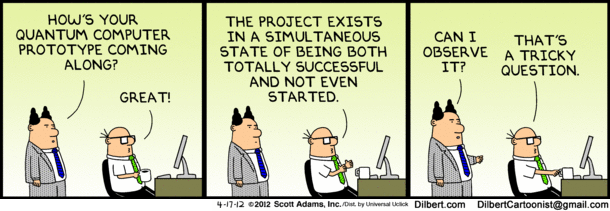
\includegraphics[width=\hsize]{images/dilbert.png}
\caption{Quanten-Computer-Projekt bei Dilbert in einem quantenmechanischen
"Uberlagerungszustand, mit besonderer Ber"ucksichtigung der Wirkung einer
Beobachtung.
\label{skript:dilbert}}
\end{figure}
Nach dem einf"uhrenden Beispiel "uber den Schr"odingerschen
Katzen-Quanten-Computer k"onnen wir uns jetzt dar"uber Gedanken
machen, wie ein Quanten-Computer aussehen m"usste, der allgemeine
mathematische Probleme l"osen k"onnte.
Ein solcher Computer existiert noch nicht, aber ein grosse Zahl von 
Forschungsgruppen (siehe auch Abbildung~\ref{skript:dilbert})
arbeiten daran, die nachstehenden Ideen auf die eine
oder andere Art umzusetzen.

Ein Quantencomputer muss zun"achst einen geeignet komplexen
"Uberlagerungszustand pr"aprieren, den Qubits. Dann muss dieser Zustand
von einem oder mehreren Quanten-Gattern verarbeitet werden, sie
entsprechen dem Operator $Q$ im Schr"odinger-Katzen-Computer.
Schliesslich muss man das Experiment mehrmals durchf"uhren, bis man
Wahrscheinlichkeiten mit gen"ugend grosser Genauigkeit bestimmt hat,
dass man ein Resultat der Berechnung daraus ableiten kann.

Ein solcher Computer bestimmt also mit beschr"ankter Wahrscheinlichkeit
in polynomieller Zeit eine L"osung f"ur ein Problem. Die
Klasse der Probleme, die sich mit beschr"ankter Wahrscheinlichkeit in
polynomieller Zeit auf einem Quantencomputer l"osen lassen, nennen wir
BQP.
Es ist klar, dass $\text{BPP}\subset\text{BQP}$.
\index{BQP, Komplexit\"atsklasse}
\index{Komplexit\"atsklasse!BQP}
Es besteht also die Hoffnung, dass sich in der Klasse BQP Probleme finden,
die ein klassischer Computer auch mit einem probabilistischen Algorithmus
nicht in polynomieller Zeit l"osen kann.

\subsection{Qubits}
Ein quantenmechanisches System mit zwei m"oglichen Zust"ande $|0\rangle$
und $|1\rangle$ muss sich nicht
notwendigerweise in genau einem der Zust"ande befinden.
Jede Linearkombination der beiden Zust"ande ist ebenfalls ein g"ultiger
Zustand, sofern sie als Vektor L"ange $1$ hat.
Der Zustand
\[
|\psi\rangle
=
\lambda \,|0\rangle + \mu\,|1\rangle
\]
hat L"ange $1$ wenn gilt
\[
\langle\psi|\psi\rangle
=
(
\bar\lambda
\langle 0|
+
\bar\mu
\langle 1|
)
(
\lambda \,|0\rangle + \mu\,|1\rangle
)
=
|\lambda|^2\langle 0|0\rangle + |\mu|^2\langle 1|1\rangle
=
|\lambda|^2+|\mu|^2
=
1
,
\]
da die gemischten Terme wegen $\langle 0|1\rangle=0$ wegfallen.
Es gen"ugt also, dass die Quadratsumme der Betr"age von $\lambda$ und $\mu$
den Wert $1$ ergibt.
Insbesondere gibt es selbst f"ur dieses einfache System bereits viel
mehr m"ogliche Zust"ande als bei einem klassischen Bit.
Ein solches quantenmechanisches System nennt man in Qubit.

Ein klassisches System mit zwei Bits kann in 4 m"oglichen Zust"anden sein.
Das zugeh"orige quantenmechanische System kann in einer beliebigen
"Uberlagerung der vier m"oglichen reinen Zust"ande sein:
\[
|\psi\rangle
=
\alpha_{00}|00\rangle
+
\alpha_{01}|01\rangle
+
\alpha_{10}|10\rangle
+
\alpha_{11}|11\rangle
,\qquad
|\alpha_{00}|^2
+
|\alpha_{01}|^2
+
|\alpha_{10}|^2
+
|\alpha_{11}|^2
=1.
\]
Wir nennen dies ein ``2-Qubit Register''.

Praktisch n"utzliche Quantencomputer m"ussen noch wesentlich gr"ossere
Qubits verarbeiten k"onnen.
Ein Register mit $n$ Qubits ist in einem Zustand, in dem $2^n$ Zust"ande
"uberlagert sind.

Es ist auch denkbar, dass wir beim Initialisieren eines Qubits
einzelne auf einen bestimmten Wert setzen.
Zum Beispiel k"onnen wir in einem Register mit $2$ Qubits das erste
Qubit auf $0$ setzen, wir erhalten dann einen Zustand der
Form
\[
|\psi\rangle
=
\alpha_{00}|00\rangle
+
\alpha_{01}|01\rangle
\]
Wir nennen das erste Bit ein Scratch-Bit.
\index{Scratch-bit}

\index{Tensor-Produkt}
Die Operation, aus einzelnen Qubits ein Register von Qubits zu
machen, ist so grundlegend, dass wir daf"ur eine eigene Notation
verwenden wollen.
Sind $H_1$ und $H_2$ die Hilbertr"aume, in denen die Zust"ande f"ur
die einzelnen Bits zu finden sind, dann schreiben wir $H_1\otimes H_2$
f"ur den Raum, der die kombinierten Zust"ande enth"alt.
Sind $|a\rangle\in H_1$ und $|b\rangle\in H_2$ Zust"ande einzelner
Qubits, dann schreiben wir f"ur den kombinierten Zustand auch
$|ab\rangle=|a\rangle\,|b\rangle=|a\rangle\otimes|b\rangle=|a\otimes b\rangle$.
Das Skalarprodukt in $H_1\otimes H_2$ ist gegeben durch
\[
\langle a\otimes b|c\otimes d\rangle
=
\langle a|c\rangle\,\langle b|d\rangle.
\]
Die Zust"ande $|0\otimes 0\rangle$,
$|0\otimes 1\rangle$,
$|1\otimes 0\rangle$ und
$|1\otimes 1\rangle$ sind dann immer noch orthogonal.

\begin{beispiel}
Man berechne das Skalarprodukt der beiden Zust"ande
\[
|\psi\rangle
=
\frac1{\sqrt{2}} |0\rangle\otimes|1\rangle
+
\frac1{\sqrt{2}} |1\rangle\otimes|0\rangle
\qquad
\text{und}
\qquad
|\varphi\rangle
=
\alpha |0\rangle\otimes|1\rangle
+
\beta |1\rangle\otimes|0\rangle.
\]
Wir k"onnen verwenden, dass die Basisvektoren $|a\otimes b\rangle$ orthogonal
sind, und schliessen, dass das Skalarprodukt
$\frac1{\sqrt{2}}\alpha + \frac1{\sqrt{2}}\beta$ sein muss.
Wir wollen uns aber "uberzeugen, dass die Definitionen ``funktionieren''
und rechnen daher das Skalarprodukt auch explizit aus.
Nach Definition des Skalarproduktes in $H_1\otimes H_2$ gilt
\begin{align*}
\langle\psi|\varphi\rangle
&=
\biggl(
\frac1{\sqrt{2}} \langle 0 \otimes 1|
+
\frac1{\sqrt{2}} \langle 1\otimes0|
\biggr)
\biggl(
\alpha |0\otimes 1\rangle
+
\beta |1\otimes 0\rangle.
\biggr)
\\
&=
\frac1{\sqrt{2}} \alpha\langle 0\otimes 1|0\otimes 1\rangle
+
\frac1{\sqrt{2}} \beta \langle 0\otimes 1|1\otimes 0\rangle
+
\frac1{\sqrt{2}} \alpha\langle 1\otimes 0|0\otimes 1\rangle
+
\frac1{\sqrt{2}} \beta \langle 1\otimes 0|1\otimes 0\rangle
\\
&=
\frac1{\sqrt{2}} \alpha\underbrace{\langle 0|0\rangle}_{=1} \underbrace{\langle 1|1\rangle}_{=1}
+
\frac1{\sqrt{2}} \beta \underbrace{\langle 0|1\rangle}_{=0} \underbrace{\langle 1|0\rangle}_{=0}
+
\frac1{\sqrt{2}} \alpha\underbrace{\langle 1|0\rangle}_{=0} \underbrace{\langle 0|1\rangle}_{=0}
+
\frac1{\sqrt{2}} \beta \underbrace{\langle 1|1\rangle}_{=1} \underbrace{\langle 0|0\rangle}_{=1}
\\
&=
\frac1{\sqrt{2}}\alpha + \frac1{\sqrt{2}}\beta,
\end{align*}
wir erhalten also genau das erwartete Resultat.
\end{beispiel}

\subsection{Gatter}
Klassische Computer f"uhren ihre Berechnung mit logischen Gattern durch,
die auf einem Vektor von Bits wirken.
Quantencomputer brauchen Quanten-Gatter, welche auf einem
$n$ Qubit Zustand wirken.
Solche Gatter d"urfen selbst keine Messungen machen, den die
Auswertung der Berechnung darf ja erst ganz am Ende der
Transformationen erfolgen.
Die Gatter sind also Zustands"anderungen, die umkehrbar sein m"ussen.
Eine physikalische Ralisierung eines Gatters ist nichts anderes
als eine Zeitentwicklung des urspr"unglichen Zustands durch einen
speziellen Hamilton-Operator.

\begin{definition}
\index{Gatter!Quanten-}
Ein Quanten-Gatter ist ein unit"arer Operator, der auf einem 
$n$-Qubit Zustand operiert.
\end{definition}

\begin{beispiel}
\index{Flip}
\index{Gatter!Flip}
Die {\em Flip Operation} implementiert die Negation eines einzelne Qubit:
\begin{align*}
|0\rangle&\mapsto |1\rangle & |1\rangle&\mapsto |0\rangle.
\end{align*}
Die zugeh"orige Matrix ist
\[
F=\begin{pmatrix}
0&1\\
1&0
\end{pmatrix}.
\]
$F$ ist eine unit"are Matrix, als ein Quanten-Gatter.
\end{beispiel}

\begin{beispiel}
\index{Bit-Umordnung}
\index{Gatter!Bit-Umordnung}
Die {\em Bit-Umordnung} vertauscht zwei Qubits, d.~h.~sie implementiert
die ABbildung:
\begin{align*}
|00\rangle&\mapsto |00\rangle\\
|01\rangle&\mapsto |10\rangle\\
|10\rangle&\mapsto |01\rangle\\
|11\rangle&\mapsto |11\rangle
\end{align*}
Die zugeh"orige Matrix ist
\[
X=
\begin{pmatrix}
1&0&0&0\\
0&0&1&0\\
0&1&0&0\\
0&0&0&1
\end{pmatrix}.
\]
Die Matrix $X$ ist unit"ar, weil orthogonal.
\end{beispiel}

\begin{beispiel}
\index{Phasenshift}
\index{Gatter!Phasenshift}
{\em Phasenshift} ist eine Operation, die den Zust"and $|1\rangle$ 
mit einem Phasenfaktor versieht:
\begin{align*}
|0\rangle &\mapsto |0\rangle\\
|1\rangle &\mapsto i\,|1\rangle
\end{align*}
Die zugeh"orige Matrix ist
\[
\begin{pmatrix}
1&0\\
0&i
\end{pmatrix},
\]
die Matrix ist nicht orthogonal, aber unit"ar.
\end{beispiel}

\begin{beispiel}
\index{Hadamard}
\index{Gatter!Hadamard}
Die {\em Hadamard-Operation} implementiert eine lineare Abbildung
\begin{align*}
|0\rangle &\mapsto |0\rangle + |1\rangle\\
|1\rangle &\mapsto |0\rangle - |1\rangle,
\end{align*}
wobei die Vektoren auf der rechten Seite noch normiert werden m"ussen.
Die zugeh"orige Matrix ist
\[
H=
\frac1{\sqrt{2}}
\begin{pmatrix}
1&\phantom{1}1\\
1&-1
\end{pmatrix}.
\]
Die Matrix $H$ ist orthogonal, also insbesondere auch unit"ar.
\end{beispiel}

\begin{beispiel}
\index{Gatter!UND}
\index{Gatter!ODER}
Es gibt weder ein UND- noch ein ODER-Gatter f"ur Quantencomputer.
Ein UND-Gatter m"usste die Abbildung
\begin{align*}
|00\rangle&\mapsto|00\rangle,\\
|01\rangle&\mapsto|00\rangle,\\
|10\rangle&\mapsto|00\rangle,\\
|11\rangle&\mapsto|01\rangle
\end{align*}
implementieren, welche nicht invertierbar ist, und daher auch nicht
unit"ar sein kann.
Selbst wenn man die Operationen UND und ODER in eine einzige Abbildung
kombiniert, erh"alt man
\begin{align*}
|00\rangle&\mapsto|00\rangle,\\
|01\rangle&\mapsto|10\rangle,\\
|10\rangle&\mapsto|10\rangle,\\
|11\rangle&\mapsto|11\rangle
\end{align*}
was immer noch nicht invertierbar ist, denn man kann aus den Resultatbits
nicht mehr schliessen, welches der beiden Bits gesetzt war.
Als letzte Hoffnung k"onnten wir versuchen, eines der Bits zu behalten,
aber das funktioniert auch nicht:
\begin{align*}
|00\rangle&\mapsto|00\rangle,\\
|01\rangle&\mapsto|00\rangle,\\
|10\rangle&\mapsto|10\rangle,\\
|11\rangle&\mapsto|11\rangle,
\end{align*}
immer noch nicht invertierbar.
\end{beispiel}

\begin{beispiel}
\index{CNOT-Gatter}
\index{Gatter!CNOT}
Das \textsc{CNOT}-Gatter invertiert das zweite Bit, wenn das erste Bit
gesetzt ist.
Es implementiert also die Abbildung
\begin{align*}
|00\rangle&\mapsto|00\rangle,\\
|01\rangle&\mapsto|01\rangle,\\
|10\rangle&\mapsto|11\rangle,\\
|11\rangle&\mapsto|10\rangle
\end{align*}
Die zugeh"orige Matrix ist
\[
U_{\textsc{CNOT}}=\begin{pmatrix}
1&0&0&0\\
0&1&0&0\\
0&0&0&1\\
0&0&1&0
\end{pmatrix}.
\]
Diese Matrix ist offensichtlich unit"ar.
Manchmal wird das \textsc{CNOT}-Gatter mit dem Diagramm
\begin{center}
\includegraphics{graphics/gatter-10.pdf}
\end{center}
dargestellt werden.
Man beachtet, dass dieses Diagramm im Gegensatz zu den Analysator-Diagrammen
von Kapitel~\ref{chapter:einfache-quantensysteme} von links nach rechts
gelesen werden m"ssen.
\end{beispiel}

\begin{beispiel}
\index{Tofoli-Gatter}
\index{Gatter!Tofoli}
Das {\em Tofoli-Gatter} operatiert auf zwei Qubits $a$ und $b$ und einem
Scratch-Bit $c$ und implementiert die Abbildung
\[
|abc\rangle
\mapsto
|a\rangle|b\rangle|(a\wedge b)\oplus c\rangle.
\]
Darin ist $\oplus$ die XOR-Operation. 
Im Detail beschreibt dies folgende Abbildung
\begin{align*}
|000\rangle&\mapsto|000\rangle\\
|001\rangle&\mapsto|001\rangle\\
|010\rangle&\mapsto|010\rangle\\
|011\rangle&\mapsto|011\rangle\\
|100\rangle&\mapsto|100\rangle\\
|101\rangle&\mapsto|101\rangle\\
|110\rangle&\mapsto|111\rangle\\
|111\rangle&\mapsto|110\rangle
\end{align*}
In dieser Reihenfolge der Basisvektoren geh"ort dazu die Matrix
\[
T=
\begin{pmatrix}
1&0&0&0&0&0&0&0\\
0&1&0&0&0&0&0&0\\
0&0&1&0&0&0&0&0\\
0&0&0&1&0&0&0&0\\
0&0&0&0&1&0&0&0\\
0&0&0&0&0&1&0&0\\
0&0&0&0&0&0&0&1\\
0&0&0&0&0&0&1&0\\
\end{pmatrix}.
\]
Die Matrix $T$ ist orthogonal, und damit auch unit"ar.
Das Tofoli-Gatter wird manchmal auch als Diagramm
\begin{center}
\includegraphics{graphics/gatter-11.pdf}
\end{center}
dargestellt. Das Zeichen \textsc{AND} erinnert daran, dass das Tofoli-Gatter
eigenlicht die UND-Verkn"upfung der beiden Inputs $a$ und $b$ berechnet.
\end{beispiel}

\begin{beispiel}
\begin{figure}
\centering
\includegraphics{graphics/gatter-12.pdf}
\caption{Implementation eines \textsc{CNOT}-Gatters aus einem Tofoli-Gatter
mit Hilfe eines Scratch-Bit \label{skript:cnot=tofoli}}
\end{figure}
Man kann aus einem Tofoli-Gatter mit Hilfe eines Scratch-Bit ein
\textsc{CNOT}-Gatter machen, wie in Abbildung~\ref{skript:cnot=tofoli}
dargestellt.
\end{beispiel}

\subsection{No-Cloning Theorem}
Ein klassischer Computer kann ein Ausgangssignal als Input f"ur viele
nachfolgende Gatter verwenden, das Bit wird einfach auf mehrere Leitungen
kopiert. 
Ein Quanten-Computer kann das nicht:
\begin{satz}
\label{skript:no-cloning-theorem}
Es gibt keine unit"are Matrix, die einen beliebigen Zustand kopieren
kann, d.~h.~die Abbildung
\[
|\psi\rangle\,|k\rangle\mapsto |\psi\rangle\,|\psi\rangle
\]
kann nicht unit"ar sein.
\end{satz}

\begin{proof}[Beweis]
Nehmen wir an, es g"abe eine unit"are Abbildung $U$, die ein Qubit clonen
kann:
\[
U(|\psi\rangle\,|k\rangle)=|\psi\rangle\,|\psi\rangle.
\]
Wenden wir $U$ auf einen analog konstruierten Zustand
$|\varphi\rangle,|k\rangle$ an, dann muss, weil $U$ unit"ar ist,
das Skalarprodukt der beiden beiden Zust"ande vor und nach der Anwendung
von $U$ gleich sein.
\begin{equation}
\left.
\begin{aligned}
\langle\varphi\otimes k|\psi\otimes k\rangle
&=
\langle\varphi|\psi\rangle \langle k|k\rangle
\\
\langle\varphi\otimes\varphi|\psi\otimes\psi\rangle
&=
\langle\varphi|\psi\rangle \langle \varphi|\psi\rangle
\end{aligned}
\quad
\right\}=
\end{equation}
Da $\langle k|k\rangle=1$ ist, folgt
\[
\langle \varphi|\psi\rangle^2=
\langle \varphi|\psi\rangle
\qquad\Leftrightarrow\qquad
\langle \varphi|\psi\rangle ( \langle \varphi|\psi\rangle -1) = 0
\qquad\Leftrightarrow\qquad
\langle \varphi|\psi\rangle =\begin{cases}0\\1\end{cases}
\]
Die beiden Zust"ande $|\psi\rangle$ und $|\varphi\rangle$ waren aber
beliebig, k"onnen also auch beliebige komplexe Zahlen als Skalarprodukt
haben.
Dieser Widerspruch zeigt, dass es eine solche Matrix $U$ gar nicht
geben kann.
\end{proof}

Qubits lassen sich also grunds"atzlich nicht kopieren.
Dies wird in der Quanten-Kryptographie zur Absicherung des
Schl"usselaustausches verwendet. 
Da der Quantenzustand, den ein Teilnehmer empf"angt, nicht kopiert
werden kann, ist es unm"oglich, den Schl"usselaustausch abzuh"oren,
ohne dass dies bemerkt wird.

\subsection{Quanten-Turing-Maschinen}
Eine Quanten-Berechnung stellt also zuerst einen Zustand in einem
Qubit-Register her.
Dann operiert darauf eine Quantenoperation, also ein unit"arer Operator $U$.
Zum Schluss finden Messungen an den einzelnen Qubits statt.
Das Resultat der Messung verr"at etwas "uber das Resultat der Berechnung.

Um einen Quantencomputer zu realisieren muss man also eine Methode
entwickeln, einen beliebigen Operator $U$ herzustellen.
In einem klassischen Computer geschieht das durch Verschaltung der
Gatter: jede beliebige logische Formal kann aus den elementaren
Gattern hergestellt werden.
F"ur Quantencomputer geht das nicht mehr exakt, das ist aber auch nicht
n"otig, wir sind ohnehin nur auf eine Approximation aus.

\begin{satz}
Jede unit"are $n\times n$-Matrix $U$ mit $n\ge 3$ kann beliebig genau
approximiert werden durch ein Produkt $U_l\dots U_1$ von unit"aren
Matrizen, die jeweils Hadamard-Gatter, Tofoli-Gatter oder Phasen-Shifts
sind.
\cite[Theorem 10.12]{skript:arorabarak}
\end{satz}

\subsection{Quanten-Algorithmen}

\section*{"Ubungsaufgaben}
\rhead{"Ubungsaufgaben}
\begin{uebungsaufgaben}
\item
\input uebungsaufgaben/04001.tex
\end{uebungsaufgaben}

\chapter{Klassische Mechanik\label{chapter:mechanik}}
\lhead{Klassische Mechanik}
\rhead{}
\section{Motivation}
\rhead{Motivation}
W"ahrend Galileo Galileis Beschreibung von Bewegungen im wesentlichen
eine kinematische war, haben Isaac
Newtons Gesetze erstmals einen Zusammenhang zwischen
der Bewegung und den Kr"aften hergestellt, also von Ursache und
Wirkung. Sein erstes Gesetz besagt zum Beispiel
\[
F=ma\qquad\text{oder}\qquad
F(x)=m\frac{d^2x}{dt^2}.
\]
Mit geeigneten Anfangsbedingungen l"asst sich daraus jede Bewegung 
vorhersagen.

Diese Formulierung ist jedoch nicht allgemein genug, insbesondere f"ur die
Zwecke der Quantenmechanik. Wenn Teilchen auch Wellen sind, wie soll man
sich dann die Kraftwirkung einer Welle auf eine andere Welle vorstellen?

Die Antwort ist die Hamiltonsche Formulierung der Mechanik, die von der
Energie als der alles bestimmenden Gr"osse ausgeht.
Mit Hilfe eines Standardformalismus lassen sich daraus die Newtonschen
Bewegungsgleichungen wieder gewinnen.
Viel wichtiger ist aber, dass sich daraus auch ein Methode gewinnen
l"asst, besonders geeignete Koordinaten zur Beschreibung eines
physikalischen Systems zu finden.
Diese Hamilton-Jacobi-Theorie genannte Methode ist die Basis eines
allgemein anwendbaren Quantisierungs-Verfahrens.

\section{Lagrange-Mechanik}
\rhead{Lagrange-Mechanik}
Das Fermatsche Prinzip besagt, dass Licht immer den Weg k"urzester Zeit
nimmt. Mit diesem Prinzip konnte Fermat sowohl das Reflexionsgesetz als
auch das Brechungsgesetz erkl"aren.
Im Lichte unserer beabsichtigen Vereinheitlichung zwischen Lichtwellen
und Teilchen sollte f"ur die Teilchenwelt ein entsprechendes Gesetz
gelten. Tats"achlich hat Pierre-Louis Maupertuis ein solches Prinzip
gefunden: ein mechanisches System entwickelt sich immer so, dass die
{\em Wirkung} minimal ist. Das Prinzip wurde von Euler, Lagrange 
und schliesslich Hamilton verallgemeinert.
\subsection{Wirkung}
Ein mechanisches System, zum Beispiel in sich bewegender Massepunkt,
wird durch eine Anzahl von Koordinaten beschrieben, die wir mit
$q_i,1\le i\le n$ bezeichnen. Die Koordinaten werden im allgemeinen 
von der Zeit abh"angen, man k"onnte also auch $q_i(t)$ schreiben.
Die Entwicklung des Systems wird durch Differentialgleichungen 
f"ur diese Funktionen $q_i(t)$ und Anfangsbedingungen beschrieben.
Zwischen den Zeitpunkten $t_0$ und $t_1$ entwickelt sich das
System
von einem Zustand $q(t_0)$ in einen Zustand $q(t_1)$.

Die Bewegung eines Teilchens wird im wesentlichen durch seine 
kinetische und potentielle Energie bestimmt. Die kinetische Energie
ist ein quadratischer Ausdruck in den Geschwindigkeiten:
\[
T=\frac12m_i\dot q_i.
\]
die potentielle Energie ist eine Funktion, die nur von der
Position des Teilchens abh"angt:
\[
V(q_1,\dots,q_n)=V(q).
\]
Die Lagrange-Funktion eines Systems ist die Differenz:
\[
L(\dot q, q) = T(\dot q) - V(q)
\]
Selbstverst"andlich ist es auch m"oglich, dass die kinetische oder
die potentielle Energie
zus"atzlich von der Zeit abh"angt, zum Beispiel "uber eine
zeitlich ver"anderliche Masse.

Die Wirkung oder Aktion einer Zeitentwicklung zwischen den Zust"anden
$q(t_0)$ und $q(t_1)$ ist die Gr"osse
\begin{equation}
W=\int_{t_0}^{t_1} L(t, q(t), \dot q(t))\,dt.
\label{skript:wirkung}
\end{equation}
Die Wirkung hangt also von der konkreten Wahl des Pfades $q(t)$ ab,
um diese Abh"angigkeit auszudr"ucken, wird manchmal auch $W[q(t)]$
geschrieben.

Das Prinzip minimaler Wirkung besagt, ein mechanisches System unter
allen m"oglichen Pfaden, die es vom Zustand $q(t_0)$ in den Zustand
$q(t_1)$ "uberf"uhren, immer denjenigen w"ahlt, f"ur die die
Wirkung minimal wird.

\subsection{Euler-Gleichungen}
Die Minimierung der Wirkung (\ref{skript:wirkung}) ist ein sogenanntes
Variationsproblem: gesucht ist ein Weg, welcher ein bestimmtes
Integral minimiert. Es ist verwandt mit der Aufgabe, den k"urzesten
Weg zu finden, der ein Gebiet mit einem bestimmten Fl"acheninhalt
umschliesst. Johann Bernoulli hat 1696 mit seinem Brachistochronen-Problem
die mathematische Welt mit einem ersten ber"uhmten Problem dieser Art
konfronriert, mit dem sich auch einige Mathematiker befasst haben.
Systematisch mit dieser Art von Problem hat sich aber erst Leonhard
Euler auseinandergesetzt, der auch einen allgemeinen L"osungsweg angegeben hat.

Gesucht wird also eine Kurve $q(t)$, welche $W[q(t)]$ minimal macht.
Jede andere Kurve, die sich nur wenig von $q(t)$ unterscheidet, sollte
daher eine gr"ossere Wirkung haben. Eine solche Nachbarkurve k"onnen
wir als
\[
q(t) + \varepsilon \eta(t)
\]
ansetzen, wobei $\eta(t)$ eine beliebig w"ahlbare Funktion ist,
die f"ur $t_0$ und $t_1$ verschwindet, $\eta(t_0)=\eta(t_1)=0$.
Wenn $q(t)$ L"osung des Minimalproblems ist, muss
\begin{equation}
\varepsilon\mapsto W[q(t)+\varepsilon\eta(t)]
\label{skript:variation-ansatz}
\end{equation}
ein Minimum f"ur $\varepsilon=0$ haben, oder die Ableitung
dieser Funktion nach $\varepsilon$ muss $0$ sein.

Setzten wir den Ansatz (\ref{skript:variation-ansatz}) in die Wirkung ein
und leiten wir nach $\varepsilon$ ab, erhalten wir
\begin{align*}
\frac{d}{d\varepsilon}W[q(t)+\varepsilon\eta(t)]
&=
\frac{d}{d\varepsilon}\int_{t_0}^{t_1}L(t, q(t)+\varepsilon\eta(t),
\dot q(t)+\varepsilon\dot\eta(t))\,dt
\\
&=\int_{t_0}^{t_1}
\frac{\partial L}{\partial q}(t, q(t)+\varepsilon\eta(t), \dot q(t)+\varepsilon\dot\eta(t))\eta(t)
+
\frac{\partial L}{\partial \dot q}(t, q(t)+\varepsilon\eta(t), \dot q(t)+\varepsilon\dot\eta(t))\dot \eta(t)\,dt.
\end{align*}
Da $q$ eigentlich ein Vektor ist, ist $\partial L/\partial q$ zu lesen
als ein Vektor bestehend aus allen Ableitungen von $L$ nach den verschiedenen
Koordinaten $q_i$, und analog f"ur $\partial L/\partial \dot q$.
F"ur $\varepsilon=0$ soll dieser Ausdruck verschwinden:
\begin{equation}
0
=\int_{t_0}^{t_1}
\frac{\partial L}{\partial q}(t, q(t), \dot q(t))\eta(t)
+
\frac{\partial L}{\partial \dot q}(t, q(t), \dot q(t))\dot \eta(t)\,dt.
\label{skript:erstevariationsgleichung}
\end{equation}
Zur Abk"urzung schreiben wir im Folgenden
\begin{align*}
\frac{\partial L}{\partial q}(t, q(t), \dot q(t))
&=
\frac{\partial L}{\partial q}
&
\frac{\partial L}{\partial \dot q}(t, q(t), \dot q(t))
&=
\frac{\partial L}{\partial \dot q}.
\end{align*}
Der zweite Term in (\ref{skript:erstevariationsgleichung}) kann mit 
partieller Integration umgeformt werden:
\begin{align*}
0
&=\int_{t_0}^{t_1}
\frac{\partial L}{\partial q}(t, q(t), \dot q(t))\eta(t)
+
\frac{\partial L}{\partial \dot q}(t, q(t), \dot q(t))\dot \eta(t)\,dt
\\
&=
\int_{t_0}^{t_1}\frac{\partial L}{\partial q}\eta(t)\,dt
+\left[
\frac{\partial L}{\partial \dot q} \eta(t)
\right]_{t_0}^{t_1}
-\int_{t_0}^{t_1}\frac{d}{dt}\frac{\partial L}{\partial \dot q}\eta(t)\,dt
\\
&=\int_{t_0}^{t_1}\left(\frac{\partial L}{\partial q}
-\frac{d}{dt}\frac{\partial L}{\partial \dot q}\right) \eta(t)\,dt.
\end{align*}
Diese letzte Gleichung ist nur dann f"ur jede beliebige Funktion $\eta(t)$
erf"ullbar, wenn der Klammerausdruck verschwindet. So erhalten wir die
Eulerschen Gleichungen f"ur das Variationsproblem.

\begin{satz}
Die Wirkung
\[
W[q(t)] =\int_{t_0}^{t_1} L(t, q(t), \dot q(t))\,dt
\]
wird minimiert von einer Funktion $q(t)$, welche den Differentialgleichungen
\[
\frac{d}{dt}\frac{\partial L}{\partial \dot q}-\frac{\partial L}{\partial q}=0
\qquad\Leftrightarrow\qquad
\frac{d}{dt}\frac{\partial L}{\partial \dot q_i}-\frac{\partial L}{\partial q_i}=0\quad\forall i
\]
gen"ugt.
\end{satz}

\subsection{Bewegungsgleichungen}
Nach Maupertuis soll das Prinzip der kleinsten Wirkung eine Bewegung
entsprechen den Newtonschen Gesetzen ergeben.
Wir wenden daher die Eulergleichungen auf das Problem eines Teilchens der
Masse $m$ in einem Potential $V(q)$ an. Die Lagrange-Funktion ist
\[
L(t, q, \dot q)=\frac12m\dot q^2-V(q).
\]
Die Ableitungen nach $q$ und $\dot q$ sind:
\begin{align*}
\frac{\partial L}{\partial \dot q}&=m\dot q=p\\
\frac{\partial L}{\partial q}&=-\frac{\partial V}{\partial q}=-\operatorname{grad}V(q).
\end{align*}
Der Ausdruck $m\dot q$ ist aus der Newtonschen Mechanik bekannt als
der Impuls eines Teilchens. Die Eulersche Gleichung wird daher zu
der Bedingung:
\[
\frac{d}{dt}\frac{\partial L}{\partial \dot q}=\frac{\partial L}{\partial q}
\qquad\Rightarrow\qquad
\frac{d}{dt}p=-\operatorname{grad}V(q).
\]
Der negative Gradient des Potentials ist die Kraft $F=-\operatorname{grad}V(q)$,
die auf das Teilchen an der Stellen $q$ wirkt.
Wir erhalten also die Newtonschen Bewegungsgleichungen.
Falls die Masse konstant ist, kann man die Ableitung nach der Zeit
noch vereinfachen, und erh"alt die wohlbekannte Form des Newtonschen
Gesetzes
\[
F= m\ddot q.
\]

Man beachte, dass diese Herleitung auch dann noch gilt, wenn die Masse von der
Zeit abh"angt (zum Beispiel bei einer Rakete).

\subsection{Fermat-Prinzip}

\section{Hamilton-Funktion}
\rhead{Hamilton-Funktion}
Die Hamilton-Funktion $H(p,q)$ ist die Energie eines physikalischen
Systems. Darin sind $q$ die allgemeinen Koordinaten, also
zum Beispiel die Raumkoordinaten $x$, $y$ und $z$, oder Winkel, mit
denen man die r"aumliche Ausrichtung eines Systems beschreibt.
Die Variablen $p$ sind die zugeh"origen Impulse, f"ur Ortskoordinaten
sind dies die gew"ohnlichen Impulskomponenten, f"ur die Drehwinkel ist
es der Drehimpuls.

Die Energie $H$ setzt sich zusammen aus der kinetischen Energie $T$ und der
potentiellen Energie $V$. F"ur ein kr"aftefreies Teilchen der Masse $m$
ist die Energie 
\[
H=\frac12mv^2=\frac1{2m}p^2.
\]
Befindet sich das Teilchen dagegen in einem Potential $V(q)$, dann 
ist die zugeh"orige Hamilton-Funktion
\begin{equation}
H=T+V=\frac1{2m}p^2+V(q).
\label{skript:hamilton-potential}
\end{equation}
Ein Elektron im elektrischen Feld eines Protons, welches im Nullpunkt
des $q$-Koordinatensystems sitzt, hat daher die Hamilton-Funktion
\[
H=\frac1{2m}p^2+\frac{e^2}{4\pi\varepsilon_0|q|}.
\]

Eine noch zu "uberwindende Schwierigkeit dieses Formalismus wird hier
bereits erkennbar: Kr"afte, die keine Arbeit leisten, k"onnen auch
keinen Beitrag zur Energie leisten.
Ein Beispiel ist
die Lorentzkraft eines Magnetfelds, welche die Bahn eines Elektrons 
kr"ummt, aber immer senkrecht auf der Bahn steht und daher keine Arbeit
leistet.

\section{Bewegungsgleichungen}
\rhead{Bewegungsgleichung}
Die Newtonschen Bewegungsgleichungen lassen sich aus der Hamilton-Funktion
gewinnen. Um dies zu verstehen, berechnen wir die partiellen Ableitungen
von $H$ nach Koordinaten $q$ und Impulsen $p$:
\begin{align*}
\frac{\partial H}{\partial p}&=\frac{1}{m}p=v=\frac{dq}{dt} \\
\frac{\partial H}{\partial q}&=\frac{\partial V}{\partial q}
\end{align*}
Die erste Gleichung ist nichts anders als die Aussage, dass die
Geschwindigkeit die Zeitableitung der Ortskoordinaten ist, sie
stellt den Zusammenhang zwischen $p$ und $q$ her.
Die Ableitung des Potentials auf der rechten Seite der zweiten
Gleichung hat die Bedeutung einer Kraft.
Die Newtonschen Bewegungsgleichungen sagen, dass die "Anderung des
Impulses durch die Kr"afte verursacht wird, also durch die Ableitungen
des Potentials:
\[
\frac{dp}{dt}=-\frac{\partial V}{\partial q}
\]
Damit sind die Bewegungsgleichungen jetzt:
\begin{align}
\frac{dq}{dt}&= \frac{\partial H}{\partial p},\label{skript:hamilton-v}\\
\frac{dp}{dt}&=-\frac{\partial H}{\partial q}.\label{skript:hamilton-newton}
\end{align}

\begin{beispiel} Harmonischer Oszillator. Ein harmonischer Oszillator
mit Masse $m$ und Federkonstante $K$ hat die potentielle Energie $\frac12Kx^2$,
die Hamilton-Funktion ist daher
\[
H=\frac1{2m}p^2+\frac12Kx^2.
\]
Die Bewegungsgleichungen nach dem Hamilton-Formalismus sind:
\begin{align*}
\frac{dx}{dt}&=\frac{\partial H}{\partial p}=\frac{p}{m}&&\Rightarrow&\dot x&=v\\
\frac{dp}{dt}&=\frac{\partial H}{\partial x}=-Kx&&\Rightarrow&ma&=-Kx
\end{align*}
Die erste Gleichung besagt, dass die Geschwindigkeit die Ableitung
der Ortskoordinate ist.
Die zweite Gleichung ist das erste Newtonsche Gesetz, denn die
r"ucktreibende Kraft einer um die Koordinate $x$ ausgelenkten Feder
mit Federkonstanten $K$ ist $-Kx$.
Insbesondere reproduziert der Hamilton-Formalismus die bekannten
Newtonschen Bewegungsgleichungen.
\end{beispiel}

Ein besonderer Fall liegt vor, wenn die Hamilton-Funktion nicht von
der Zeit abh"angt. Dann ist
\[
\frac{\partial H}{\partial t}=0,
\]
die Energie ist erhalten. Diese Situation tritt in abgeschlossenen
Systemen immer auf, insbesondere waren alle bisherigen Beispiel
von dieser Art.

\section{Kanonische Transformation}
\rhead{Kanonische Transformation}
Kartesische Koordinaten sind nicht unbedingt die optimale Wahl.
Eine zweckm"assige Wahl der Koordinaten nimmt R"ucksicht auf die
Symmetrieeigenschaften des Systems.
Ein zweidimensional rotationssymmetrischer harmonischer Oszillator mit 
der Hamilton-Funktion
\[
H=\frac1{2m}(p_x^2+p_y^2)+K(x^2 + y^2)
\]
sollte sich auch in Polarkoordinaten $(r,\varphi)$ ausdr"ucken lassen. 
Doch welche Impulse sind dann zu verwenden, damit die Gleichungen
(\ref{skript:hamilton-v}) und (\ref{skript:hamilton-newton}) auch in den neuen
Koordinaten G"ultigkeit haben?

\section{Hamilton-Jacobi-Theorie}
\rhead{Hamilton-Jacobi-Theorie}
Die Technik der kanonischen Transformationen erlaubt sogar, ein mechanisches
Problem mit Hilfe einer geeigneten Transformation vollst"andig zu l"osen.
Wie dies funktionieren k"onnte zeigt ein Vergleich mit einem freien
Teilchen, also der Hamilton-Funktion
\[
H=\frac1{2m}(p_x^2+p_y^2+p_z^2).
\]
Da die Koordinaten $x$, $y$ und $z$ gar nicht vorkommen, verschwinden
die Ableitungen von $H$ nach den Koordinaten und die Bewegungsgleichungen
sind
\begin{align*}
\frac{dp}{dt}&=0\\
\frac{dq}{dt}&=\frac{p}{m}
&&\Rightarrow&q=q_0+t\frac{p}{m}
\end{align*}
Die Ortskoordinaten h"angen linear von der Zeit ab.

\section{Wellen und Teilchen}
\rhead{Welle und Teilchen}

\section{Bedeutung des Hamilton Operators}
\rhead{Bedeutung des Hamilton-Operators}

\chapter{Quantisierung\label{chapter:quantisierung}}
\lhead{Quantisierung}
\rhead{}

\section{Quantisierungsregeln}
\rhead{Quantisierungsregeln}
\index{Quantisierungsregel}%
In diesem Abschnitt untersuchen wir, wie ein klassisches System, dessen
Beschreibung wir bereits kennen, in ein quantenmechanisches System 
mit dem Formalismus aus Kapitel~\ref{chapter:einfache-quantensysteme}
umgeformt werden kann.
Dabei m"ussen alle klassisch beobachtbaren Gr"ossen, also alle Obervablen
wie Position, Impuls, Energie etc.~erhalten erhalten bleiben.

In der Bohrschen Quantenmechanik wurde gefordert, dass 
sich Teilchen auf Bahnen bewegen m"ussen, f"ur die eine
Quantisierungsbedingung gilt.
\index{Quantisierungsbedingung von Bohr}%
Typischerweise musste das Produkt $p\dot q$ entlang einer geschlossenen
Bahn aufintegriert ein ganzzahliges Vielfaches von $\hbar$ ergeben.
Dieses Quantisierungsprinzip geht davon aus, dass man immer noch sinnvoll
von einer Bahn sprechen kann, was wir aber schon ausgeschlossen haben.
Wir m"ussen daher ein Quantisierungsprinzip verwenden, welches den
Begriff einer Bahn gar nicht erst verwendet, sondern nur Dinge, die
auch tats"achlich beobachtbar sind, also Observable.

In der klassischen Mechanik sind Observable einfach Funktionen
der Koordinaten und Impulse,
in der Quantenmechanik werden sie durch selbstadjungierte
Operatoren dargestellt.
Um die klassischen Observablen von den Operatoren unterscheiden zu
k"onnen, werden wir in diesem Abschnitt die Operatoren mit einem
Circumflex kennzeichnen.
Der Hamilton-Operator wird also mit $\hat H$ bezeichnet, 
\index{Hamilton-Operator}%
der Operator zur klassischen Variable $X$ wird mit $\hat X$ etc.

\subsection{Zeitentwicklung}
\index{Zeitentwicklung}%
In Abschnitt~\ref{section:zeitentwicklung-von-observablen} haben wir die
Zeitentwicklung eines Quantensystems kennengelernt.
Wir nehmen an, dass der Hamilton-Operator $H$ nicht von der Zeit abh"angt.
Sei $\hat A$ eine Observable, und sei $|\psi(t)\rangle$ der Zustand des
Quantensystems zur Zeit $t$.
Dann gilt
\[
\frac{d}{dt}\langle \hat A\rangle
=
\biggl\langle -\frac{i}{\hbar}[\hat A,\hat H] \biggr\rangle.
\]
Als Spezialfall muss darin die Bewegung eines klassischen mechanischen Systems
enthalten sein, wie wir es in Kapitel~\ref{chapter:mechanik}
kennengelernt haben.
Ein solches System zeichnet sich dadurch aus, dass die {\em Wellenfunktion}
\label{Wellenfunktion}
$\Psi(x,t)=\langle x|\psi(t)\rangle$
\index{Wellenfunktion}%
sehr gut lokalisiert ist.
\index{de Broglie, Louis}%
Nach de~Broglie werden Quantenph"anomene nur auf einer Entfernung sichtbar,
die der de~Broglie-Wellenl"ange $\lambda=h/p$ des Teilchens entsprechen.
Weiter als einige de~Broglie-Wellenl"angen von $\langle x\rangle$
entfernt wird $\Psi$ verschwinden.
\index{de Broglie-Wellenlange@de Broglie-Wellenl\"ange}%

Eine Observable $A$ des klassischen Systems ist eine Funktion der
Koordinaten und Impulse, man kann ihre Zeitentwicklung mit den
Bewegungsgleichungen~\ref{skript:zeitentwicklung-poisson}
berechnen:
\[
\frac{d}{dt}A=(A,H).
\]
Die Quantisierungsregel lautet daher:

\begin{satz}
\label{skript:quantisierung-poisson}
\index{Quantisierungsregel!mit Poisson-Klammern und Kommutatoren}%
Ein klassisches System mit Hamilton-Funktion $H$ wird quantisiert, indem
jede Observable $A$ durch einen Operator $\hat A$ ersetzt wird, die
Hamilton-Funktion durch einen Hamilton-Operator $\hat H$, und jede
Poisson-Klammer durch einen Kommutator nach der Regel
\begin{equation}
(A,B)
\qquad
\mapsto
\qquad
-\frac{i}{\hbar}[\hat A,\hat B].
\label{skript:quantisierung-observable}
\end{equation}
\end{satz}
Aus den Regeln folgt auch, dass der Operator $\hat H$ tats"achlich
der Operator ist, der der klassischen Observablen $H$ entspricht, also der 
Energie des Systems.
\label{skript:hamilton-op-ist-energie}

\subsection{Ortsdarstellung}
\index{Ortsdarstellung}%
Klassische Systeme werden in Koordinaten und Impulsen beschrieben, 
die nat"urlich auch Observable sind.
Ausserdem k"onnen wir den Zustandsvektor in der Ortsdarstellung
als Wellenfunktion $\Psi(x,t)=\langle x|\psi(t)\rangle$
ausdr"ucken.
Statt mit den abstrakten Vektoren $|\psi\rangle$ zu rechnen, m"ochten
wir mit den viel konkreteren Wellenfunktionen $\Psi(x,t)$ rechnen 
k"onnen. Wir m"ussen also alle Operationen mit $|\psi\rangle$ neu
als Operationen auf $\Psi(x,t)$ ausdr"ucken.

Nach den allgemeinen Grunds"atzen des fr"uher entwickelten Formalismus
muss $|\Psi(x,t)|^2$ die Wahrscheinlichkeitsdichte f"ur die Position
des Teilchens sein.
\index{Wahrscheinlichkeitsdichte eines Teilchens}%
F"ur zwei verschiedene Zust"ande muss das Skalarprodukt daher als
\index{Skalarprodukt}%
\index{Skalarprodukt!in Ortsdarstellung}%
Integral gebildet werden:
\[
\left.
\begin{aligned}
\Psi(x,t)&=\langle x|\psi\rangle\\
\Phi(x,t)&=\langle x|\varphi\rangle
\end{aligned}
\quad
\right\}
\qquad
\Rightarrow
\qquad
\langle\varphi|\psi\rangle
=
\int \langle\varphi|x\rangle\langle x|\psi\rangle\,dx
=
\int \overline{\langle x| \varphi\rangle}\langle x|\psi\rangle\,dx
=
\int \bar\Phi(x,t)\Psi(x,t)\,dx.
\]

Wir erinnern daran, wie Erwartungswerte zu berechnen sind.
\index{Erwartungswert}%
F"ur eine klassische  Observable $G$, die nur vom Ort eines Teilchens abh"angt,
muss f"ur den Erwartungswert gelten
\[
\langle G\rangle = \int G(x)\cdot |\Psi(x,t)|^2\,dx
=
\int\bar\Psi(x,t)\,G(x)\,\Psi(x,t)\,dx.
\]
Der in der Ortsdarstellung zu $G$ geh"orige Operator ist also nichts
anderes als die Multiplikation mit $G(x)$.

Doch wie muss man den Operator f"ur den Impuls ausdr"ucken?
Um die Wirkung von $\hat p$ zu ermitteln, verwenden wir die
Quantisierungsregeln.
F"ur eine klassische Observable $G(x)$, die nur von $x$
abh"angt, gilt
\begin{equation}
(p,G)=-\frac{\partial G}{\partial x}.
\label{skript:pGobservable}
\end{equation}
Wir wenden jetzt die
Quantisierungsvorschrift~(\ref{skript:quantisierung-observable})
auf (\ref{skript:pGobservable}) an und erhalten
\[
\begin{CD}
\displaystyle(p,G)     @=   \displaystyle-\frac{\partial G}{\partial x}.\\
@V\text{Quantisierung}VV           @V\text{Quantisierung}VV   \\
\displaystyle-\frac{i}{\hbar}[\hat p,\hat G]
@=
\displaystyle-\widehat{\frac{\partial G}{\partial x}}.\\
@V\textstyle\langle\,.\,\rangle VV           @V\textstyle\langle\,.\,\rangle VV   \\
\displaystyle -\int \bar\Psi(x,t)\,\biggl(\frac{i}{\hbar}\hat p G(x)-G(x)\frac{i}{\hbar}\hat p\biggr)\,\Psi(x,t)\,dx
@=
\displaystyle -\int \bar \Psi(x,t)\,\frac{\partial G}{\partial x}\,\Psi(x,t)\,dx
\end{CD}
\]
Man beachte, dass in der letzten Gleichung auf der linken Seite der Operator
$\hat p$ auf das Produkt $G(x)\Psi(x,t)$ wirkt.
Damit daraus eine Ableitung von $G$ entstehen kann, muss der Operator
$\hat p$ selbst wie eine Ableitung operieren. Setzen wir
\begin{equation}
\frac{i}{\hbar}\hat p = \frac{\partial}{\partial x},
\label{skript:praeimpulsoperator}
\end{equation}
wird die letzte Gleichung zu
\begin{align}
-\int \bar\Psi(x,t)\,\biggl(\frac{\partial}{\partial x}G(x)-G(x)\frac{\partial}{\partial x}\biggr)\,\Psi(x,t)\,dx
&=
-\int \bar \Psi(x,t)\,\frac{\partial G}{\partial x}\,\Psi(x,t)\,dx
\notag
\\
-\int \bar\Psi(x,t)\,\biggl(
\frac{\partial G}{\partial x}
+
G(x)\frac{\partial}{\partial x}
-G(x)\frac{\partial}{\partial x}\biggr)\,\Psi(x,t)\,dx
&=
-\int \bar \Psi(x,t)\,\frac{\partial G}{\partial x}\,\Psi(x,t)\,dx.
\label{skript:produktregelpG}
\end{align}
Darin haben wir die Produktregel auf das Produkt $G(x)\Psi(x,t)$ angewendet.
Offenbar war (\ref{skript:praeimpulsoperator}) die richtige Wahl, und wir
haben eine vereinfachte Quantisierungsregel f"ur die Ortsdarstellung
gefunden.

\begin{satz}
\label{skript:quantisierungsregeln-ortsdarstellung}
\index{Quantisierungsregel!in Ortsdarstellung}
Ein mechanisches System wird in der Ortsdarstellung quantisiert,
indem als Impulsoperatoren die Differentialoperatoren
\[
\hat p=\frac{\hbar}{i}\frac{\partial}{\partial x}
\]
verwendet werden. Den Hamilton-Operator $\hat H$ erh"alt man, indem man
in der Hamilton-Funktion $H$ die Variablen $p$ durch die Operatoren 
$\hat p$ ersetzt.
\end{satz}

{\small
Alternativ kann man die Quantisierungsregel f"ur den Impulsoperator
auch wie folgt verstehen.
\index{Quantisierungsregel!Impulsoperator}%
Die Anwendung der Produktregel in (\ref{skript:produktregelpG}) kann
man auch als eine Anwendung der partiellen Integration ansehen.
Wir berechnen dazu direkt den Erwartungswert von $\partial G/\partial x$:
\begin{align*}
\biggl\langle
\frac{\partial G}{\partial x}
\biggr\rangle
&=
\int \bar\Psi(x,t)\frac{\partial G(x)}{\partial x}\Psi(x,t)\,dx
\\
&=
\underbrace{
\biggl[
\bar\Psi(x,t) G(x)\Psi(x,t)
\biggr]_{-\infty}^\infty}_{=0}
-
\int_{-\infty}^{\infty}
\biggl(\frac{\partial}{\partial x}
\bar\Psi(x,t)\biggr) G(x)
\Psi(x,t)
+
\bar\Psi(x,t) G(x)
\,
\frac{\partial}{\partial x}
\Psi(x,t)
\,dx
\\
&=
\int_{-\infty}^{\infty}
\biggl(-\frac{\partial}{\partial x}
\bar\Psi(x,t)\biggr) G(x)
\Psi(x,t)
-
\bar\Psi(x,t) G(x)
\,
\frac{\partial}{\partial x}
\Psi(x,t)
\,dx
\\
&=\biggl\langle
\biggl(-\frac{\partial}{\partial x}\biggr)^* G
- G\frac{\partial}{\partial x}
\biggr\rangle
\end{align*}
%Der Ableitungsoperator mit dem $\mathstrut^*$ in der letzten Zeile
%wirkt auf die Wellenfunktion links. Dieser Operator ist nicht
%hermitesch, vielmehr gilt
%\begin{align*}
%\biggl\langle \varphi\bigg|\,
%\biggl(\frac{\partial}{\partial x}\biggr)^*
%\,\bigg|\psi\biggr\rangle
%&=
%\int \frac{\partial\bar\Phi(x,t)}{\partial x}\Psi(x,t)\,dx
%%\\
%%&=
%\underbrace{
%\biggl[\bar\Phi(x,t)\Psi(x,t)\biggr]_{-\infty}^\infty
%}_{=0}
%-
%\int \bar\Phi(x,t)\frac{\partial\Psi(x,t)}{\partial x}\,dx
%=
%-\biggl\langle
%\varphi\bigg|\,
%\frac{\partial}{\partial x}
%\,\bigg|\psi
%\biggr\rangle
%\end{align*}
Setzt man jetzt wieder (\ref{skript:praeimpulsoperator}) ein, erh"alt
man daraus
\[
\biggl\langle
\frac{\partial G}{\partial x}
\biggr\rangle
=
\biggl\langle
\biggl(-\frac{i}{\hbar}\hat p
\biggr)^* G
- G\frac{i}{\hbar}\hat p
\biggr\rangle
=
\frac{i}{\hbar}
\biggl\langle
\hat p
 G
- G \hat p
\biggr\rangle
=
\frac{i}{\hbar}[\hat p,G],
\]
was wieder mit der Quantisierung der klassischen Beziehung
\ref{skript:pGobservable} "ubereinstimmt.
}

\section{Schr"odingergleichung}
\rhead{Schr"odingergleichung}
In diesem Abschnitt leiten wir aus den Quantisierungsregeln die
Schr"odingergleichung her, welche uns erm"oglicht, einfache
Quantensysteme mit Differentialgleichungen zu modellieren
und zum Beispiel die Energieniveaus und Wellenfunktionen direkt
zu berechnen.

\subsection{Schr"odingergleichung in Ortsdarstellung}
\index{Schrodingergleichung@Schr\"odingergleichung!in Ortsdarstellung}
Wir wenden die vereinfachten Quantisierungsregeln auf ein
Teilchen in einem Potential an.
Dieses hat die Hamilton-Funktion
\[
H=\frac1{2m}p^2+V(x).
\]
Nach den Quantisierungsregeln in
Satz~\ref{skript:quantisierungsregeln-ortsdarstellung} wird daraus
der Hamilton-Operator:
\index{Hamilton-Operator!in Ortsdarstellung}
\[
\hat H
=
\frac{1}{2m}\biggl(\frac{\hbar}{i}\frac{\partial }{\partial x}\biggr)^2
+V(x)
=
-\frac{\hbar^2}{2m}\frac{\partial^2}{\partial x^2}+V(x).
\]
In drei Dimension treten entsprechend mehr Ableitungen auf:
\[
H=\frac1{2m}\sum_{i=1}^3p_i^2+V(x)
\qquad\Rightarrow\qquad
\hat H
=
-\frac{\hbar^2}{2m}\sum_{i=1}^3\frac{\partial^2}{\partial x_i^2}+V(x)
=
-\frac{\hbar^2}{2m}\Delta + V(x).
\]
Die zugeh"orige zeitabh"angige Schr"odingergleichung ist
\[
i\hbar\frac{\partial}{\partial t}\Psi(x,t)
=
-\frac{\hbar^2}{2m}\Delta\Psi(x,t) + V(x)\Psi(x,t).
\]
\index{Schrodingergleichung@Schr\"odingergleichung!zeitabh\"angige}
Ein Teilchen mit Energie $E$ in einem Potential $V(x)$ wird entsprechend
durch eine Wellenfunktion $\Psi(x)$ beschrieben, die zeitunabh"angige
Schr"odingergleichung
\[
-\frac{\hbar^2}{2m}\Delta\Psi(x) + V(x)\Psi(x)
=
E\Psi(x)
\]
erf"ullt.
Ausserdem m"ussen die Wellenfunktionen nat"urlich normiert sein.
\index{normiert}%

Damit lassen sich jetzt einfache Potential-Probleme l"osen.
Wir untersuchen im Folgenden die Bewegung eines Teilchens in einfachen
Potentialen, um erste Erfahrungen mit der Schr"odingergleichung
zu sammeln und einen ersten Eindruck von den Eigenheiten der
des quantenmechanischen Verhaltens von Teilchen zu erhalten.

\subsection{Potentialkasten\label{subsection:potentialkasten}}
\index{Potentialkasten}
Wir wenden die Theorie an, um die Energieniveaus eines eindimensionalen
Teilchens zu berechnen, welches in einem Interval $[-l,l]$ eingesperrt ist.
Realisiert werden kann diese Situation n"aherungsweise dadurch, dass 
ein Teilchen durch eine sehr hohe (unendlich hohe) Potentialbarriere
am verlassen des Bereiches gehindert wird.
Die Wellenfunktion $\psi(x)$ eines solchen Teilchens muss ausserhalb des
Intervals verschwinden, denn die Wahrscheinlichkeit, das Teilchen dort zu
finden, soll ja $0$ sein.
Man erreicht dies, indem man in den Punkten $\pm l$ eine unendlich
hohe Potentialbarriere errichtet.

\subsubsection{Hamilton-Operator und Schr"odingergleichung}
Der Hamilton-Operator des Problems ist
\[
-\frac{\hbar^2}{2m}\frac{\partial^2}{\partial x^2}+V(x),
\]
das Potential hat die Form
\[
V(x)=\begin{cases}
0&\qquad |x|<l\\
\infty&\qquad\text{sonst.}
\end{cases}
\]
Die zugeh"orige zeitunabh"angige Schr"odingergleichung ist
\begin{equation}
-\frac{\hbar^2}{2m}\psi''(x)=E\psi(x)
\label{skript:schroedingerkasten}
\end{equation}
im Inneren des Intervals.
Wir suchen eine L"osung von (\ref{skript:schroedingerkasten}),
die ausserdem den Randbedingungen
\[
\psi(\pm l)=0
\]
gen"ugen soll, damit wird dem unendlich hohen Potential ausserhalb des
Kastens Rechnung getragen.
Das charakteristische Polynom der Gleichung (\ref{skript:schroedingerkasten}) ist
\[
-\frac{\hbar^2}{2m}\lambda^2-E=0,
\]
es hat die Nullstellen
\[
\lambda_\pm = \pm\sqrt{\frac{2m}{\hbar^2}(-E)}.
\]

\subsubsection{Symmetrie}
\index{Spiegelung}
Der Hamilton-Operator dieses Problems ist symmetrisch bez"uglich
der Spiegelung.
Der Spiegelungsoperator $S$, der aus der Wellenfunktion
$\psi(x)$ die Wellenfunktion $\psi(-x)$ macht, vertauscht mit
dem Hamilton-Operator, also kann man die Eigenzust"ande von $H$ so w"ahlen,
dass sie auch Eigenzust"ande von $S$ sind.
Da $S^2=\operatorname{id}$, sind $\pm1$ die einzig m"oglichen Eigenwerte
von $S$, also ist $\psi(x)=\psi(-x)$ oder $\psi(x)=-\psi(-x)$.
Wenn man eine L"osung der Schr"odingergleichung sucht, kann man also
zus"atzlich verlangen, dass die L"osungen gerade oder ungerade Funktionen
sind.

\subsubsection{Negative Energie}
Falls $E<$ ist, sind die Nullstellen des chrakteristischen
Polynoms reell, $\lambda_+>0$ und $\lambda_-=-\lambda_+ < 0$,
und die allgemeine 
L"osung der Gleichung (\ref{skript:schroedingerkasten}) hat die Form
\[
\psi(x)=A_+e^{\lambda_+x}+A_-e^{\lambda_-x}.
\]
Ausserdem m"ussen die Randbedingungen erf"ullt sein, die man erh"alt,
indem man $x=\pm l$ setze:
\[
\begin{linsys}{2}
e^{ \lambda_+l} A_+&+&e^{ \lambda_-l}A_-&=&0\\
e^{-\lambda_+l}A_+&+&e^{-\lambda_-l}A_-&=&0
\end{linsys}
\]
Dieses Gleichungssystem f"ur die Koeffizienten $A_+$ und $A_-$ hat
Determinante
\[
\left|\begin{matrix}
e^{ \lambda_+l}&e^{ \lambda_-l}\\
e^{-\lambda_+l}&e^{-\lambda_-l}
\end{matrix}\right|
=
e^{\lambda_+l-\lambda_-l}-e^{\lambda_-l-\lambda_+l}
=
e^{2l\lambda_+}-e^{-2l\lambda_+}
=
2\sinh 2l\lambda_+
\]
Dieses Ausdruck verschwindet nur, wenn $\lambda_+=0$, im Widerspruch
zu $\lambda_+>0$.
Es gibt also keine L"osung f"ur Teilchen mit negativer Energie.

\subsubsection{Positive Energie}
In diesem Falls sind die Nullstellen imagin"ar, $\lambda_\pm=\pm ik$
mit $k=\sqrt{2mE/\hbar^2}$,
und die allgemeine L"osung wird durch Linearkombinationen der Funktionen
$\cos kx$ und $\sin kx$ gegeben.
Wir m"ussen also herausfinden, f"ur welche Werte von $E$ und damit $k$
die Randbedingungen erf"ullt werden k"onnen.
Wir wissen bereits, dass wir zus"atzlich verlangen k"onnen, dass die
L"osungen gerade oder ungerade sind.
Eine gerade L"osung muss von der Form $A\cos kx$ sein, eine ungerade
L"osung von der Form $B\sin kx$.
In beiden F"allen ist die Randbedingung am linken Rand automatisch
erf"ullt, wenn die Bedingun am rechten Rand erf"ullt ist.
Wir setzen die Randbedingungen ein:
\begin{align*}
A\cos kl&=0
	&&&
		B\sin kl&=0\\
kl&=\frac{\pi}2+n\pi,\quad n\in\mathbb Z
	&&&
		kl&=n\pi,\quad n\in\mathbb Z\\
k&=\frac{\pi}{l}\biggl(n+\frac12\biggr),\quad n\in\mathbb Z
	&&&
		k&=\frac{\pi}{l}n,\quad n\in\mathbb Z.
\end{align*}
Es sind also alle $k$-Werte m"oglich, die ganzzahlige Vielfache von
$\pi/2l$ sind.
Die geraden Vielfache f"uhren zu einer $\sin$-L"osung, die ungeraden
zu einer $\cos$-L"osung.

Aus den m"oglichen $k$-Werten k"onnen wir jetzt die m"oglichen 
Energiewerte ableiten
\begin{align*}
E&=\frac{\hbar^2\pi^2}{2ml^2}\biggl(n+\frac12\biggr)^2
&&&
E&=\frac{\hbar^2\pi^2}{2ml^2}n^2
\end{align*}
In einer Formel zusammengefasst kann man schreiben
\[
E_n
=
\frac{\hbar^2\pi^2}{2ml^2}\biggl(\frac{n}{2}\biggr)^2
=
\frac{h^2n^2}{32ml^2}.
\label{skript:potentialkasten-e}
\]
wobei f"ur gerades $n$ eine ungerade L"osungsfunktion auftritt,
f"ur ungerades $n$ aber eine gerade L"osungsfunktion.
\begin{figure}
\centering
\includegraphics{graphics/potential-1.pdf}
\caption{Teilchen in einem Potentialkasten
\label{skript:potentialkasten}}
\end{figure}

\subsubsection{Normierung}
Wir m"ussen noch sicherstellen, dass die L"osungsfunktionen korrekt
normiert sind.
Dazu m"ussen wir die Integrale von $\cos^2$ und $\sin^2$ berechnen.
Die Graphen von $\cos^2$ und $\sin^2$ halbieren aber genau das
Rechteck zwischen $-l$ und $l$ mit H"ohe $1$, also ist der Wert
des Integrals in jedem Fall $l$, die L"osungsfunktionen mit
der richtigen Normierung sind also:
\begin{align}
\psi_n(x)
&=
\begin{cases}
\displaystyle
\frac{1}{\sqrt{l}}\cos\frac{n \pi x}{2l}&\qquad \text{$n$ ungerade}\\
\\
\displaystyle
\frac{1}{\sqrt{l}}\sin\frac{n \pi x}{2l}&\qquad \text{$n$ gerade}.
\end{cases}
\label{skript:potentialkasten-psi-normiert}
\end{align}
Der Grundzustand ist $n=1$, mit Grundzustandsenergie $E_1=h^2/32ml^2$.

\subsubsection{Klassische Quantisierungsbedingung}
Klassisch kann man sich das Teilchen als eine Welle vorstellen, die
zwischen den beiden W"anden des Potentialkastens hin und her l"auft.
Der Impuls des Teilchens ist $\hbar k$, die Wirkung f"ur einen Weg
hin und zur"uck ist daher:
\[
\oint p\,dq
=
2\cdot \hbar k \cdot 2l = 2\cdot \hbar \frac{\pi}{l}\frac{n}{2}\cdot 2l=hn,
\]
dies entspricht genau der Bohrschen Quantisierungsbedingung.

\subsubsection{Physikalische Interpretation}
Offenbar ist es nicht m"oglich, auf beliebig kleinem Raum einzusperren.
Je kleiner der zur Verf"ugung stehende Raum, desto h"oher ist die
Energie, die ein Teilchen mindestens haben wird.
Im Kapitel~\ref{chapter:heisenberg} werden wir mit der Unsch"arferelationen
einen weiteren Ausdruck dieses Ph"anomens kennenlernen.

In einem Atomkern sind die Protonen und Neutronen auf sehr kleinem
Raum eingesperrt, und wir k"onnen versuchen, die minimale Energie 
eines Neutrons abzusch"atzen.
Der Atomkern hat einen Durchmesser von $10\text{fm}=10\cdot 10^{-15}\text{m}$,
das Neutron hat eine Masse von $m_n=1.67\cdot 10^{-27}\text{kg}$,
die Grundzustandsenergie ist daher $E_1=3.28\cdot10^{-13}\text{J}$.
Mit der Formel $E=mc^2$ entspr"ache dieser Energie die Masse
$3.656\cdot 10^{-30}\text{kg}$, oder etwa $0.2\%$ der Masse eines
Neutrons, und mehr als der Masse eines Elektrons.

\subsubsection{H"ohere Dimensionen}
Man kann das Problem eines Teilchens in einem Potentialkasten auch
in drei Dimensionen l"osen.
Der Hamiltonoperator ist 
\[
H=-\frac{\hbar^2}{2m}\biggl(
\frac{\partial^2}{\partial x^2}
+
\frac{\partial^2}{\partial y^2}
+
\frac{\partial^2}{\partial z^2}
\biggr)
=-\frac{\hbar^2}{2m}\Delta
\]
Man verwendet dazu einen sogenannten Seprationsansatz, man schreibt
\[
\psi(x,y,z)=X(x)\cdot Y(y)\cdot Z(z),
\]
und erh"alt die Differentialgleichung
\[
\frac{\hbar^2}{2m}\biggl(
X''(x)Y(y)Z(z)
+
X(x)Y''(y)Z(z)
+
X(x)Y(y)Z''(z)
\biggr)
=
EX(x)Y(y)Z(z)
\]
Dividiert man durch $\psi$, erhalt man die Gleichung
\begin{equation}
-\frac{\hbar^2}{2m}\frac{X''(x)}{X(x)}
-
\frac{\hbar^2}{2m}\frac{Y''(y)}{Y(y)}
-
\frac{\hbar^2}{2m}\frac{Z''(z)}{Z(z)}
=
E.
\label{skript:potentialkasten-separiert}
\end{equation}
Man kann nach jedem Term aufl"osen, und erh"alt dann eine Gleichung,
deren linke Seite nur von einer Variablen, die rechte nur von den anderen
abh"angt.
Es folgt dann, dass beide Seiten konstant sein m"ussen, 
die Gleichung (\ref{skript:potentialkasten-separiert}) beinhaltet also eigentlich
drei Gleichungen
\begin{equation}
\begin{aligned}
-\frac{\hbar^2}{2m}\frac{X''(x)}{X(x)}&=E_x&&\Rightarrow&-\frac{\hbar^2}{2m}X''&=E_xX\\
-\frac{\hbar^2}{2m}\frac{Y''(y)}{Y(y)}&=E_y&&\Rightarrow&-\frac{\hbar^2}{2m}Y''&=E_yY\\
-\frac{\hbar^2}{2m}\frac{Z''(z)}{Z(z)}&=E_z&&\Rightarrow&-\frac{\hbar^2}{2m}Z''&=E_zZ
\end{aligned}
\label{skript:potentialkasten-einzelgleichungen}
\end{equation}
mit der zus"atzlichen Bedingung $E=E_x+E_y+E_z$.
Die Gleichungen (\ref{skript:potentialkasten-einzelgleichungen}) sind drei
unabh"angige Problem wie der eindimensionale Potentialkasten
(\ref{skript:schroedingerkasten}), deren Energieniveaus wir bereits berechnet
haben.
Daraus k"onnen wir unmittelbar die Energieniveaus im dredimensionalen
Fall ableiten:
\begin{equation}
E=\frac{h^2}{32ml^2}(n_x^2+n_y^2+n_z^2)
\label{skript:3dzustaende}
\end{equation}
mit $n_x,n_y,n_z>1$.


\subsection{Potentialtopf}
Aus der L"osung des Problems eines Teilchens in einem Potentialkasten
k"onnte der Eindruck entstehen, dass die Quantisierung der Energieniveaus
mit der Randbedingung am Rande des Kastens zu tun hat.
Sobald diese Bedingung wegf"allt, k"onnten die Bedingungen nicht mehr
ausreichend streng sein, um diskrete Energieniveaus zu erzwingen.
Dass dem nicht so ist zeigt das hier zu behandelnde Beispiel eines
Teilchens in einem Potentialtopf, wie auch der sp"ater im
Kapitel~\ref{chapter:harmonisch} behandelte harmonische Oszillator.

\subsubsection{Problemstellung}
\begin{figure}
\centering
\includegraphics{graphics/potential-2.pdf}
\caption{Potentialtopf der Breite $2l$ und Tiefe $-V_0$.
\label{potentialtopf}}
\end{figure}

Wir m"ochten die Schr"odingergleichung l"osen f"ur ein Teilchen, welches
dem in Abbildung~\ref{potentialtopf} festgehalten wird.
Das Potential ist
\[
V(x)
=
\begin{cases}
-V_0&\qquad|x|<l\\
0&\qquad\text{sonst}
\end{cases}
\]
Die Schr"odingergleichung lautet
\[
-\frac{\hbar^2}{2m}\psi''(x)+V(x)\psi(x)=E\psi(x).
\]
Die L"osungsfunktion $\psi(x)$ muss also je nach Teilinterval
verschiedene Differentialgleichungen l"osen:
\begin{equation}
\begin{aligned}
-\frac{\hbar^2}{2m}\psi''(x)&=(V_0+E)\psi(x)&\text{f"ur $|x|\le l$}
\\
-\frac{\hbar^2}{2m}\psi''(x)&=E\psi(x)      &\text{f"ur $|x|>l$}
\end{aligned}
\label{potentialtopf-gleichungen}
\end{equation}
Wir werden die Differentialgleichung in jedem dieser Teilintervalle
separat l"osen, und dann zu einer Funktion $\psi$ zusammensetzen.
Die Funktion $\psi(x)$ muss nat"urlich stetig sein, die einzelnen
Teile m"ussen also an den Stellen $x=\pm l$ ohne Sprung ineinander
"ubergehen.
Dasselbe muss f"ur die Ableitungen gelten, denn wenn $\psi'$  nicht
stetig w"are, w"urde die zweite Ableitung unendlich gross, was nicht
mit der Schr"odingergleichung vereinbar ist.

\subsubsection{L"osungen von (\ref{potentialtopf-gleichungen})}
Die Gleichungen sind von der Form
\begin{equation}
\psi''(x)=C\psi(x),\qquad
C=-\frac{2m}{\hbar^2}(V_0+E)
\;
\text{oder}
\;
C=-\frac{2m}{\hbar^2}E,
\label{potentialtopf-proto}
\end{equation}
die wir mit dem Standardverfahren f"ur lineare Differentialgleichungen
l"osen k"onnen.
Die charakteristische  Gleichung ist $\lambda^2=C$, mit Nullstellen
$\lambda=\sqrt{C}$. Je nach Vorzeichen von $C$ ist der Charakter der
L"osungen verschieden.
F"ur $C>0$ sind die $e^{x\sqrt{C}}$ und $e^{-x\sqrt{C}}$.

F"ur $C<0$ sind die L"osungen der charakterisischen Gleichung imagin"ar.
Man kann die L"osungen der Differentialgleichung mit Exponentialfunktionen
$e^{ix\sqrt{-C}}$ und $e^{-ix\sqrt{-C}}$ schreiben.
Es wird aber viel einfacher, wenn man wieder die Symmetrieeigenschaften
verwendet, und nach geraden und ungeraden L"osungsfunktionen sucht,
die sich mit $\cos x\sqrt{-C}$ bzw.~$\sin x\sqrt{-C}$ schreiben
lassen m"ussen.

\subsubsection{F"alle $E>0$ und $E<-V_0$}
F"ur $E>0$ sind die L"osungen "uberall Schwingungsl"osungen, deren
Amplitude auf der ganzen reellen Achse ausserhalb des Topfes
konstant ist. Eine solche Funktion ist nicht normierbar, insbesondere
kann es f"ur $E>0$ also keine L"osungen geben.

F"ur $E<-V_0$ ist das $C>0$ in (\ref{potentialtopf-proto}), es kommen
also nur die Exponentialfunktionen f"ur eine L"osung in Frage.
Damit l"asst sich aber keine normierbare L"osung bauen: rechts von $l$
d"urfte man nur $e^{-x\sqrt{C}}$ verwenden, links von $-l$ nur
$e^{-x\sqrt{C}}$, und dazwischen m"usste man ein Funktion konstruieren,
die an den R"andern stetig differenzierbar in die beiden abfallenden
Exponentialfunktionen "ubergeht.
Dies scheitert am gleichen Gleichungssystem wie beim Potentialkasten
im Falle $E<0$.

\subsubsection{Der Fall $-V_0 < E < 0$}
In diesem Fall suchen wir jetzt eine gerade oder ungerade L"osung, die
im Interval $[-l,l]$ eine Schwingungsl"osung $a \cos kx$ oder $a \sin kx$
ist mit 
\[
k=\sqrt{\frac{2m}{\hbar^2}(V_0+E)},
\]
und f"ur $x>l$ eine exponentiell abfallende L"osung $be^{k'(x-l)}$
mit
\[
k'=\sqrt{-\frac{2m}{\hbar^2}E}.
\]
Wegen der Symmetrie reicht es jetzt, die Bedingungen nur noch beim
Punkt $l$ aufzustellen.
Die Stetigkeitsbedingungen lauten 
\begin{align*}
&&\psi(-x)&=\psi(x)	&	\psi(-x)&=-\psi(x)\\
&\text{Stetigkeit von $\psi$ bei $x=l$:}&
	a\cos kl&= b	&	a\sin kl&=b \\
&\text{Stetigkeit von $\psi'$ bei $x=l$:}&
	-ak\sin kl&=-bk'&     ak\cos kl&=-bk'
\end{align*}
Dividiert man die beiden Gleichungen, erhalten wir zwei
Gleichungen, die nur noch $k$ und $k'$ enthalten:
\begin{align}
\tan kl&=\frac{k'}{k},
&-\cot kl&=\frac{k'}{k},
\label{potentialtopf-k-gleichungen}
\end{align}
Die Gr"ossen $k$ und $k'$ h"angen aber beide von $E$ ab, dies sind
als in Wirklichkeit Gleichungen f"ur $E$.

\begin{figure}
\centering
\includegraphics[width=\hsize]{graphics/potential-4.pdf}
\caption{L"osungen der Gleichungen (\ref{potentialtopf-xigleichungen}).
Rote Kurve: $\sqrt{A^2-\xi^2}/\xi$, blaue Kurven: $\tan\xi$, gr"une
Kurven $-\cot\xi$.
\label{loesungen-xigleichungen}}
\end{figure}%
\begin{figure}
\centering
\includegraphics{graphics/potential-5.pdf}
\caption{Wellenfunktionen f"ur Teilchen in einem Potentialtopf der
Tiefe $-V_0$ under der Breite $2l$. Nur die sechs Wellenfunktionen 
geringster Energie sind dargestellt, und die Energie "uber dem
Grund des Potentialtopfes ist 15fach "uberh"oht.
\label{potentialtopf-loesungen-klein}}
\end{figure}
\begin{figure}
\centering
\includegraphics{graphics/potential-3.pdf}
\caption{Wellenfunktionen f"ur Teilchen in einem Potentialtopf der
Tiefe $-V_0$ under der Breite $2l$. Die Wellenfunktionen zu den sechs
untersten Energieniveaus sind nicht dargestellt, siehe dazu die
Abbildung~\ref{potentialtopf-loesungen-klein}.
\label{potentialtopf-loesungen}}
\end{figure}
Wir versuchen, alle Gr"ossen durch die dimensionslose Gr"osse $\xi=kl$
auszudr"ucken.
Zun"achst ist
\begin{align}
\xi=kl&=l\sqrt{\frac{2m}{\hbar^2}(V_0+E)}
\notag
\\
\xi^2
&=
\frac{2ml^2}{\hbar^2}(V_0+E)
=
\frac{2ml^2V_0}{\hbar^2} +\frac{2ml^2}{\hbar^2}E
=
\frac{2ml^2V_0}{\hbar^2}-l^2k'^2
\notag
\\
k'l
&=
\sqrt{\frac{2ml^2V_0}{\hbar^2} - \xi^2}
\notag
\\
E
&=
-\frac{\hbar^2}{2m}k'^2
=
-\frac{\hbar^2}{2m}
\biggl(
\frac{2mV_0}{\hbar^2} - \frac{\xi^2}{l^2}
\biggr)
=
-V_0+\frac{\hbar^2\xi^2}{2ml^2}
\label{potentialtopf-energie}
\end{align}
Schreiben wir
\[
A=\sqrt{\frac{2ml^2V_0}{\hbar^2}}
\]
und setzen wir ein in die Gleichungen (\ref{potentialtopf-k-gleichungen}),
erhalten wir die neuen Gleichungen f"ur $\xi$
\begin{align}
\tan \xi&=\frac{\sqrt{A^2-\xi^2}}{\xi}
&
-\cot \xi&=\frac{\sqrt{A^2-\xi^2}}{\xi}
\label{potentialtopf-xigleichungen}
\end{align}
In Abbildung~\ref{loesungen-xigleichungen} sind die rechten und linken
Seiten der Gleichungen (\ref{potentialtopf-xigleichungen}) aufgezeichnet,
die Schnittpunkte geh"oren zu $\xi$-Werten, f"ur die es L"osungen
der Schr"odingergleichung gibt.
Die zugeh"origen Energien k"onnen mit (\ref{potentialtopf-energie})
berechnet werden.


Die Gleichungen (\ref{potentialtopf-xigleichungen}) k"onnen nicht 
in geschlossener Form gel"ost werden, die Energieniveaus k"onnen also
nur numerisch bestimmt werden.
Man kann immerhin ein paar qualitative Aussagen machen.
Aus Abbildung~\ref{loesungen-xigleichungen} kann man ablesen, dass die
$\xi$-Werte f"ur die Niveaus mit niedrigester Energie nahe an $n\pi/2$
sind, die Energien sind also nahe bei
\[
-V_0+\frac{\hbar^2\xi^2}{2ml^2}
\simeq
-V_0+\frac{h^2n^2\pi^2}{32ml^2\pi^2}
=
-V_0+\frac{h^2n^2}{32ml^2},
\]
die Energie dieser Niveaus liegt also "ahnlich hoch "uber dem Grund
des Potentialtopfes, wie wir f"ur einen Potentialkasten gefunden haben.

Die L"osungsfunktionen sind in den
Abbildungen~\ref{potentialtopf-loesungen-klein}
und \ref{potentialtopf-loesungen}
dargestellt.
Man erkennt, dass man die Teilchen mit positiver Wahrscheinlichkeit in
der Wand antreffen wird, die Eindringtiefe ist zudem umso gr"osser,
je gr"osser die Energie eines Teilchens ist.


\section{Wahrscheinlichkeitsstrom}
% Kontinuitätsgleichung für die Wahrscheinlichkeitsdichte <psi(x)|psi(x)>
Die Wahrscheinlichkeit ein Teilchen in einer Umgebung des
Punktes $x$ zu finden, ist $\varrho(x)=\langle \psi(x)|\psi(x)\rangle$.
Die Zeitentwicklung f"uhrt dazu, dass $\varrho$ auch von der
Zeit abh"angt.
Die gesamte Wahrscheinlichkeit muss nat"urlichh erhalten bleiben,
das Teilchen kann ja nicht einfach verschwinden.

Wenn sich mit der Zeitentwicklung das Teilchen woanders hin bewegt,
dann ist damit ein Stromdichtevektor verbunden, der angibt, 
wieviel Wahrscheinlichkeit durch eine Fl"ache fliesst.
Das Ziel dieses Abschnittes ist, eine solche Stromdichte zu
definieren.

\subsection{Kontinuit"atsgleichung}
\index{Kontinuit\"atsgleichung}%
Wir stellen uns ein Medium mit Dichte $\varrho(x,t)$ vor.
Das Medium hat im Punkt $x$ die Str"omungsgeschwindigkeit $v(x)$.
In einem Zeitinterval $\Delta t$ nimmt die Masse des Mediums
in einem Interval der L"ange $\Delta x$ um den Betrag
\[
\Delta x\frac{\partial\varrho}{\partial t}\Delta t
\]
zu.
Dies Zunahme muss dadurch erfolgen, dass durch die Endpunkte
des $\Delta x$-Intervals mehr Material zu- als abfliesst.
Der Zufluss am linken Ende des Intervals ist
$
\varrho(x) v(x),
$
der Abfluss am rechten Ende ist $\varrho(x+\Delta x)v(x+\Delta x)$.
Die Bilanz ist
\[
\Delta x\frac{\partial\varrho}{\partial t}\Delta t
=
\Delta t(
\varrho(x) v(x)
-
\varrho(x+\Delta x) v(x+\Delta x)
)
\]
Wir teilen durch $\Delta x\,\Delta t$ und lassen $\Delta x$ gegen 0 gehen:
\begin{equation}
\frac{\partial\varrho}{\partial t}
+\frac{\partial}{\partial x}(\varrho(x)v(x))
=0.
\label{skript:kontinuitaetsgleichung1d}
\end{equation}
Die Gr"osse $j(x)=\varrho(x)v(x)$ beschreibt den Materialstrom.
Die Gleichung (\ref{skript:kontinuitaetsgleichung1d}) heisst die
{\em Kontinuit"atsgleichung}.
\index{Kontinuitatsgleichung@Kontinuit\"atsgleichung}
Sie dr"uckt aus, dass im Verlauf der Str"omung kein Material verlorgen
gehen kann.

In drei Dimensionen kann man ebenfalls ein Kontinuit"atsgleichung
f"ur die Dichte $\varrho(x)$ und den Strom $\vec j(x)=\varrho(x) \vec v(x)$
definieren, die die dreidimensionale 
Kontinuit"atsgleichung
\[
\frac{\partial\varrho}{\partial x}
+
\frac{\partial j_1}{\partial x_1}
+
\frac{\partial j_2}{\partial x_2}
+
\frac{\partial j_3}{\partial x_3}
=
\frac{\partial\varrho}{\partial t}+\operatorname{div}\vec j
=0
\]
erf"ullt.

\subsection{Wahrscheinlichkeitsstrom}
Wir suche jetzt einen Wahrscheinlichkeitsstrom, der zusammen mit
der Wahrscheinlichkeitsdichte $|\psi(x)|^2$ eine Kontinuit"atsgleichung
erf"ullt.
\begin{align*}
\frac{\partial\varrho(x,t)}{\partial t}
&=
\frac{\partial}{\partial t} \varrho(x)
=
\frac{\partial\varrho(x)}{\partial t}
=
\frac{\partial\overline{\psi(x,t)}}{\partial t}\psi(x,t)
+
\overline{\psi}(x,t)\frac{\partial\psi(x,t)}{\partial t}
\end{align*}
Im letzten Term k"onnen wir die Zeitableitungen durch die
Schr"odingergleichung ersetzen:
\begin{align*}
\frac{\partial\varrho(x,t)}{\partial t}
&=
\frac{\partial\overline{\psi(x,t)}}{\partial t}\psi(x,t)
+
\overline{\psi}(x,t)\frac{\partial\psi(x,t)}{\partial t}
\\
&=
\overline{ \frac{i}{\hbar}H \psi(x,t) }\psi(x,t)
+
\overline{\psi}(x,t)\frac{i}{\hbar} H \psi(x,t)
\\
&=
-
\frac{\hbar^2}{2m}\overline{\frac{\partial^2\psi(x,t)}{\partial x^2}}\psi(x,t)
+
\frac{\hbar^2}{2m}\frac{\partial^2\psi(x,t)}{\partial x^2}\overline{\psi(x,t)}
+
V(x)|\psi(x,t)|^2
\end{align*}
Die ersten zwei Terme k"onnen wir auch als Ableitung
der Funktion
\[
j(x,t)=
\frac{\hbar^2}{2m}
\biggl(
-\frac{\partial\overline{\psi}(x,t)}{\partial x}\psi(x,t)
+\overline{\psi}(x,t)\frac{\partial\psi(x,t)}{\partial x}
\biggr)
\]
erhalten, denn
\begin{align*}
\frac{\partial j(x,t)}{\partial x}
&=
\frac{\hbar^2}{2m}
\frac{\partial}{\partial x}
\biggl(
-\frac{\partial\overline{\psi}(x,t)}{\partial x}\psi(x,t)
+\overline{\psi}(x,t)\frac{\partial\psi(x,t)}{\partial x}
\biggr)
\\
&=
\frac{\hbar^2}{2m}
\biggl(
-
\frac{\partial^2\overline{\psi}(x,t)}{\partial x^2}
\psi(x,t)
-
\frac{\partial\overline{\psi}(x,t)}{\partial x}
\frac{\partial\psi(x,t)}{\partial t}
+
\frac{\partial\overline{\psi}(x,t)}{\partial x}
\frac{\partial\psi(x,t)}{\partial x}
+
\overline{\psi}(x,t)
\frac{\partial^2\psi(x,t)}{\partial x^2}
\biggr)
\\
&=
\frac{\hbar^2}{2m}
\biggl(
-
\frac{\partial^2\overline{\psi}(x,t)}{\partial x^2}
\psi(x,t)
+
\overline{\psi}(x,t)
\frac{\partial^2\psi(x,t)}{\partial x^2}
\biggr)
\end{align*}
Somit erf"ullt die oben definierte Funktion $j(x,t)$ die
Kontinuit"atsgleichung
\[
\frac{\partial\varrho(x,t)}{\partial t}
=
\frac{\partial j(x,t)}{\partial x} +V(x)\varrho(x,t).
\]

\section*{"Ubungsaufgaben}
\rhead{"Ubungsaufgaben}
\begin{uebungsaufgaben}
\item
Quantisieren Sie das mechanische System mit der klassischen Hamilton-Funktion
\[
H(x,p)=\frac{1}{2m}p^2+ax^4.
\]
Berechnen Sie auch den Kommutator von $x$ mit dem Hamilton-Operator in
der Ortsdarstellung.

\begin{loesung}
Nach den Quantisierungsregeln in
Satz~\ref{skript:quantisierungsregeln-ortsdarstellung}
muss die Variable $p$ durch den Differentialoperator
\[
\hat p=\frac{\hbar}{i}\frac{\partial}{\partial x}
\]
ersetzt werden.
Man erh"alt
\[
\hat H
=
-\frac{\hbar^2}{2m}\frac{\partial^2}{\partial x^2}+ax^4
\]
als Hamilton-Operator.
Den Kommutator $[x,\hat H]$ in der Ortsdarstellung ermitteln wir durch 
seine Wirkung auf eine Wellenfunktion $\psi(x)$:
\begin{align*}
[x,\hat H]\psi(x)
&=
x\biggl(
-\frac{\hbar^2}{2m}\frac{\partial^2}{\partial x^2}+ax^4
\biggr)\psi(x)
-
\biggl(
-\frac{\hbar^2}{2m}\frac{\partial^2}{\partial x^2}+ax^4
\biggr)x\psi(x)
\\
&=
-\frac{\hbar^2}{2m}\biggl(
x\psi''(x)
-
x\psi''(x)
-
2\psi'(x)
\biggr)
=
\frac{\hbar^2}{m}\psi'(x)
=
-\frac{\hbar}{i}\frac1{m}\frac{\hbar}{i}\frac{\partial}{\partial x}\psi(x)
=
-\frac{\hbar}{i}\frac1{m}\hat p\psi(x).
\end{align*}
Zu Beginn der zweiten Zeile brauchen wir die Beziehung
\[
\frac{\partial^2}{\partial x^2}(x\psi(x))
=
\frac{\partial}{\partial x}\biggl(
\psi(x)+x\psi'(x)
\biggr)
=
\psi'(x)+\psi'(x)+x\psi''(x)
=
x\psi''(x)+2\psi'(x).
\]
Die Quantisierungsregeln aus Satz~\ref{skript:quantisierung-poisson}
besagen, dass Kommutatoren mit Poisson-Klammern in Beziehung stehen:
\begin{align*}
-\frac{i}{\hbar}
[x,\hat H]
&=
\frac1{m}\hat p.
\end{align*}
Der Operator auf der rechten Seite ist der Operator f"ur die
Geschwindigkeit,
und tats"achlich muss der Kommutator mit $\hat H$ ja die Zeitwentwicklung
der Observablen $x$ ausdr"ucken.
\end{loesung}


\item
Man berechne die Energieniveaus eines Teilchens der Masse $m$ in einem
Potential $V(x)=v|x|$.

\begin{loesung}
Die Quantisierungsregeln f"uhren auf die Schr"odingergleichung
\[
-\frac{\hbar^2}{2m}\psi''(x)+v|x|\psi(x)=E\psi(x).
\]
Wir k"onnen die L"osung $\psi(x)$ f"ur die ganze relle Achse gewinnen,
indem wir eine L"osung f"ur positive $x$ gerade oder ungerade
auf die negative reelle Achse fortsetzen. 
Ersteres funktioniert nur, wenn $\psi'(0)=0$ ist, zweites nur
wenn $\psi(0)=0$.

Wenn wir aber nur L"osungen f"ur $x>0$ suchen, dann k"onnen wir
auf das Betragszeichen verzichten.
Wir suchen also L"osungen der Differentialgleichung
\begin{equation}
-\frac{\hbar^2}{2m}\psi''(x)+vx \psi(x)=E\psi(x),
\label{06002:dgl}
\end{equation}
die f"ur $x\to\infty$ beschr"ankt bleiben und die oder deren Ableitung
bei $x=0$ verschwindet.
\begin{table}
\centering
\begin{tabular}{|>{$}c<{$}|>{$}c<{$}|}
\hline
n&x_n\\
\hline
\phantom{0}1&-\phantom{0}1.018793\\
\phantom{0}2&-\phantom{0}2.338107\\
\phantom{0}3&-\phantom{0}3.248198\\
\phantom{0}4&-\phantom{0}4.087949\\
\phantom{0}5&-\phantom{0}4.820099\\
\phantom{0}6&-\phantom{0}5.520560\\
\phantom{0}7&-\phantom{0}6.163307\\
\phantom{0}8&-\phantom{0}6.786708\\
\phantom{0}9&-\phantom{0}7.372177\\
10&-\phantom{0}7.944134\\
11&-\phantom{0}8.488487\\
12&-\phantom{0}9.022651\\
13&-\phantom{0}9.535449\\
14&-10.040174\\
15&-10.527660\\
16&-11.008524\\
17&-11.475057\\
18&-11.936016\\
\hline
\end{tabular}
\caption{Nullstellen von $\operatorname{Ai}(x)$ und den
Ableitungen $\operatorname{Ai}'(x)$.
F"ur $n$ ungerade ist $x_n$ eine Nullstelle von $\operatorname{Ai}'(x)$,
f"ur $n$ gerade eine von $\operatorname{Ai}(x)$.
\label{skript:airy-nullstellen}}
\end{table}

Die Differentialgleichung kann durch Verschiebung des Arguments $x$ 
und durch Skalierung in die Form
\[
y''-xy=0
\]
gebracht, werden, die Airysche Differentialgleichungen. 
\index{Airy!Differentialgleichung}
Ihre L"osungen sind Linearkombinationen der Airy-Funktionen
\index{Airy!Funktion}
$\operatorname{Ai}(x)$ und $\operatorname{Bi}(x)$ (siehe zum Beispiel
\cite{skript:airy})..
Da $\operatorname{Bi}(x)$ f"ur $x\to\infty$ unbeschr"ankt
w"achst, darf $\operatorname{Bi}(x)$ in der L"osung nicht
vorkommen.
Daraus folgt, dass die L"osung bis auf die Normierung von der
Form
\[
\psi(x)=\operatorname{Ai}(ax-b)
\]
sein muss.
Dies setzen wir jetzt in die Differentialgleichung~(\ref{06002:dgl}) ein,
und erhalten die Gleichung
\begin{align*}
-\frac{\hbar^2}{2m}a^2\operatorname{Ai}''(ax-b)
+
vx\operatorname{Ai}(ax-b)
&=
E\operatorname{Ai}(ax-b)
\\
-\frac{\hbar^2}{2m}a^2(ax-b)\operatorname{Ai}(ax-b)
+
vx\operatorname{Ai}(ax-b)
&=
E\operatorname{Ai}(ax-b)
\\
-\frac{\hbar^2}{2m}a^2(ax-b)
+
vx
&=
E
\end{align*}
Beide Seiten dieser Gleichung sind Polynome, durch Koeffizientenvergleich
finden wir daher die Bedingungen f"ur $a$ und $b$
\begin{align*}
-\frac{\hbar^2}{2m}a^3+v&=0
&
-\frac{\hbar^2}{2m}a^2b&=E
\\
\Rightarrow\qquad
a &= \biggl(\frac{\hbar^2}{2mv}\biggr)^{-\frac13}
&
\Rightarrow\qquad
b &= -\frac{E}{v}\biggl(\frac{\hbar^2}{2mv}\biggr)^{1-\frac23}
= -\frac{E}{v}\biggl(\frac{\hbar^2}{2mv}\biggr)^{-\frac13}
\end{align*}
Damit die L"osung f"ur $x>0$ sich zu einer L"osung f"ur alle $x$
erweitern l"asst, muss $\psi(0)=0$ oder $\psi'(0)=0$ sein,
es muss also $b$ eine Nullstelle von $\operatorname{Ai}(x)$ oder
von $\operatorname{Ai}'(x)$ sein.
Sind $x_n$ die Nullstellen von $\operatorname{Ai}(x)$ und
$\operatorname{Ai}'(x)$ mit $x_{n+1}<x_n$, dann sind die zugeh"origen
Energieniveaus:
\[
E_n=v\root 3\of{\frac{\hbar^2}{2mv}} x_n.
\]
Auch die Wellenfunktionen kann man angeben.
F"ur ungerade $n$ ist $x_n$ eine Nullstelle von $\operatorname{Ai}'(x)$,
die Wellenfunktion ist gerade:
\begin{equation}
\psi(x)
=
\operatorname{Ai}\biggl( \root3\of{\frac{2mv}{\hbar^2}}(|x|-x_n) \biggr).
\end{equation}
F"ur gerade $n$ ist $x_n$ eine Nullstelle von $\operatorname{Ai}(x)$
und die Wellenfunktion ist ungerade
\begin{equation}
\psi(x)
=
\begin{cases}
\displaystyle
\phantom{-}\operatorname{Ai}\biggl( \root3\of{\frac{2mv}{\hbar^2}} (x-x_n)\biggr)
	&\qquad x\ge 0\\
\displaystyle
-\operatorname{Ai}\biggl( \root3\of{\frac{2mv}{\hbar^2}}(x-x_n)\biggr)
	&\qquad x < 0
\end{cases}
\end{equation}
\begin{figure}
\centering
\includegraphics{graphics/linear-1.pdf}
\caption{Wellenfunktionen eines Teilchens in einem linearen Potential.
\label{skript:linear-wave-functions}}
\end{figure}%
In Abbildung~\ref{skript:linear-wave-functions} sind die Wellenfunktionen
f"ur die ersten 18 Energieniveaus dargestellt.
Die zugeh"origen Nullstellen sind in der Tabelle~\ref{skript:airy-nullstellen}
zusammengestellt.
Je h"oher die Energie eines Zustands ist, desto h"oher ist die Frequenz
der Wellenfunktion in der N"ahe von $0$.
Da die Differenz zwischen aufeinanderfolgenden Nullstellen immer kleiner
wird, werden auch die Differenzen zwischen den Energieniveaus immer kleiner.
\end{loesung}


\end{uebungsaufgaben}



\chapter{Heisenbergsche Unsch"arferelation\label{chapter:heisenberg}}
\lhead{Heisenbergsche Unsch"arferelation}
\rhead{}

In der Quantenmechanik lassen sich die Observablen nicht mehr einfach
vertauschen, wie das in der klassischen Mechanik m"oglich war.
F"ur Operatoren gilt im Allgemeinen kein Kommutativgesetz.
In diesem Abschnitt wollen wir die Konsequenzen dieser Tatsache
untersuchen.
Wir k"onnen aber bereits jetzt feststellen, dass die Gleichung
$AB=BA$ f"ur zwei quantenmechanische Observable ``fast'' stimmen
muss, in dem Sinne, dass der Unterschied der beiden Seiten sehr
klein sein muss. 

\section{Vertauschungsrelationen und Eigenvektoren}
\rhead{Vertauschungsrelationen und Eigenvektoren}
%\subsection{Definitionen}
\index{Kommutator}
\index{Antikommutator}
Zu zwei Operatoren $A$ und $B$ kann man Kommutator und Antikommutator
bilden:
\[
\begin{aligned}
&\text{Kommutator:}&
[A,B]&=AB-BA
\\
&\text{Antikommutator:}&
\{A,B\}&=AB+BA
\end{aligned}
\]
Wenn $[A,B]=AB-BA=0$ folgt $AB=BA$,
der Kommutator gibt also an, ob die beiden Operatoren vertauschen (kommutieren).
Wenn $\{A,B\}=AB+BA=0$ folgt $AB=-BA$,
der Kommutator gibt also an, ob die beiden Operatoren antikommutieren.

\subsection{Kommutator und Eigenvektoren}
Falls $A$ and $B$ Observable sind, die nicht vertauschen, dann k"onnen
gemeinsame Eigenvektoren nicht beliebig sein.

\begin{hilfssatz}
\label{skript:kommutatorannihliertev}
Der Kommutator $[A,B]$ annihiliert gemeinsame Eigenvektoren von $A$ und $B$.
\end{hilfssatz}

\begin{proof}[Beweis]
Nehmen wir an, $|\psi\rangle$ sei ein gemeinsamer Eigenvektor
von $A$ mit Eigenwert $\alpha$ und $B$ mit Eigenwert $\beta$.
Dann wirkt der Kommutator auf $|\psi\rangle$ wie folgt
\[
[A,B]\,|\psi\rangle
=
(AB-BA)\,|\psi\rangle 
=
A\beta\,|\psi\rangle -B\alpha\,|\psi\rangle
=
\alpha\beta\,|\psi\rangle-\beta\alpha\,|\psi\rangle
=
0.
\]
Ein gemeinsamer Eigenvektor $|\psi\rangle$ wird also von $[A,B]$
zu $0$ gemacht.
\end{proof}

In vielen F"allen ist der Kommutator ein Vielfaches der identischen
Abbildung. F"ur diese F"alle l"asst sich eine etwas sch"arfere
Folgerung ableiten.

\begin{satz}
Wenn zwei Observable einen Kommutator haben, der ein Vielfaches
der identischen Abbildung ist, dann haben die Observable keine
gemeinsamen Eigenvektoren.
\end{satz}

\begin{beispiel}
F"ur die Observablen $X$ f"ur Ort und $P$ f"ur den Impuls eines Teilchens,
k"onnen wir den Kommutator in der Ortsdarstellung explizt ausrechnen:
\begin{align*}
[X,P]\psi(x)
&=
\biggl[
x,\frac{\hbar}{i}\frac{\partial}{\partial x}
\biggr]\psi(x)
=
x\frac{\hbar}{i}\frac{\partial\psi(x)}{\partial x}
-
\frac{\hbar}{i}\frac{\partial}{\partial x}\bigl(x\psi(x)\bigr)
\\
&=
x\frac{\hbar}{i}\frac{\partial\psi(x)}{\partial x}
-
\frac{\hbar}{i}\psi(x)
-
\frac{\hbar}{i}x\frac{\partial\psi(x)}{\partial x}
=
-\frac{\hbar}{i}\psi(x).
\end{align*}
Der Kommutator ist also
\[
[X,P]=-\frac{\hbar}{i}\operatorname{id},
\]
ein Vielfaches der identischen Abbildung.
Die identische Abbildung hat nat"urlich keine Vektoren, die von ihr
annihiliert werden.
Orts- und Impuls-Operatoren k"onnen also keine gemeinsamen Eigenvektoren
haben.
\end{beispiel}

\subsection{Eigenbasen von zwei Operatoren}
Umgekehrt stellt sich die Frage, unter welchen Voraussetzungen zwei
Observable eine Basis von gemeinsamen Eigenvektoren haben k"onnen.
Der n"achste Satz liefert ein Kriterium daf"ur.

\begin{satz}
\label{skript:kommevbasis}
Wenn zwei selbstadjungierte Operatoren vertauschen, dann gibt es eine
gemeinsame Basis von Eigenvektoren.
\end{satz}

\begin{proof}[Beweis]
Wir f"uhren den Beweis nur f"ur einen endlichdimensionalen Zustandsraum.
Seien also $A$ und $B$ zwei selbstadjungierte Operatoren mit $[A,B]=0$.
Ist $v$ ein Eigenvektor von $A$ zum Eigenwert $a$, dann gilt
$ Av=av $.
F"ur den Vektor $Bv$ gilt dann
\[
A(Bv)=BAv=Bav=aBv,
\]
$Bv$ ist also ebenfalls ein Eigenvektor von $A$ zum gleichen Eigenwert.
F"ur einen Eigenvektor $u$ von $B$ gilt analog, dass $Au$ ein Eigenvektor
von $B$ zum gleichen Eigenwert ist.

Zu jedem Eigenwert $a$ von $A$ sie $E_a$ der Raum der von den 
Eigenvektoren von $A$ zum Eigenwert $a$ aufgespannte Vektorraum.
$E_a$ heisst Eigenraum von $A$ zum Eigenwert $a$.
Nach Satz~\ref{skript:evorthogonal} sind die Eigenr"aume $E_a$ 
f"ur verschiedene $a$ orthogonal, und in jedem Eigenraum wirkt $A$
wie das $a$-fache der Einheitsmatrix.

Es gibt nur endliche viele verschiedene Eigenwert $a_1,\dots,a_k$.
Bildet man eine Basis des Zustandsraumes, indem man in jedem $E_{a_i}$
eine Basis w"ahlt, dann bekommt $A$ die Form
\[
A=\left(
\begin{array}{ccccccccccc}
a_1   &\dots &0     &      &      &      &      &      &      &      &      \\
\vdots&\ddots&\vdots&      &      &      &      &      &      &      &      \\
0     &\dots &a_1   &      &      &      &      &      &      &      &      \\
%\hline
      &      &      &a_2   &\dots &0     &      &      &      &      &      \\
      &      &      &\vdots&\ddots&\vdots&      &      &      &      &      \\
      &      &      &0     &\dots &a_2   &      &      &      &      &      \\
%\hline
      &      &      &      &      &      &\ddots&      &      &      &      \\
      &      &      &      &      &      &      &\ddots&      &      &      \\
%\hline
      &      &      &      &      &      &      &      &a_k   &\dots &0     \\
      &      &      &      &      &      &      &      &\vdots&\ddots&\vdots\\
      &      &      &      &      &      &      &      &0     &\dots &a_k   
\end{array}
\right)
\]

Weiter oben wurde gezeigt, dass der Operator $B$ die Eigenr"aume $E_a$ in sich
abbildet: $BE_a\subset E_a$. Da $B$ ausserdem selbstadjungiert ist, kann man
in jedem Eigenraum $E_{a_i}$ eine Basis
${\cal B}_i= \{b_1^{(i)},\dots,b_{l_i}^{(i)}\}$
aus Eigenvektoren f"ur $B$ finden. Die Vektoren $b_j^{(i)}$ sind nach
Konstruktion sowohl Eigenvektoren von $A$ zum Eigenwert $a_i$ als auch
Eigenvektoren von $B$. Die Vereinigung
\[
{\cal B}
=
\bigcup_{i=1}^k{\cal B}_i
=
\{
b_1^{(1)},\dots,b_{l_1}^{(1)},
b_1^{(2)},\dots,b_{l_2}^{(2)},
\dots,
b_k^{(k)},\dots,b_{l_k}^{(k)}
\}
\]
der Basen ${\cal B}_i$ ist eine Basis des Zustandsraumes aus gemeinsamen
Eigenvektoren von $A$ und $B$, in ihr haben beide Operatoren Diagonalform.
\end{proof}

\begin{satz}
Zwei Observablen haben genau dann eine gemeinsame Basis aus Eigenvektoren,
wenn sie vertauschen.
\end{satz}

\begin{proof}[Beweis]
Aus Satz~\ref{skript:kommevbasis} leiten wir ab, dass das Kriterium
gen"ugend ist.
Der Kommutator $[A,B]$ annihiliert gemeinsame Eigenvektoren von $A$
und $B$.
G"abe es eine Basis aus Eigenvektoren, dann m"usste der Kommutator alle
Basisvektoren annihilieren, es folgte $[A,B]=0$. Dieser
Widerspruch zeigt, dass das Kriterium auch notwendig ist.
\end{proof}


\section{Unscharfe Kenntnis von Observablen}
\rhead{Unscharfe Kenntnis von Observablen}
Im Allgemeinen kann man nicht annehmen, dass ein Beobachtung einer
Observablen $A$ im Zustand $|\psi\rangle$ immer den gleichen Wert ergibt.
Die Messwerte werden zum Beispiel wegen der unvermeidlichen
Unzul"anglichkeiten der Messung streuen.
Dann ist der Erwartungswert $\langle \psi|\,A\,|\psi\rangle$
der Observablen $A$ im Zustand $|\psi\rangle$ die genaueste Information,
die wir erhalten k"onnen.
Zur Abk"urzung schreiben wir $\langle A\rangle=\langle\psi|\,A\,|\psi\rangle$.
Mit $A$ ist auch $A-\langle A\rangle$ eine Observable, und ihr Erwartungswert
ist nat"urlich $0$.

Damit stellt sich die Frage, ob man f"ur spezielle Zust"ande eventuell
mehr Information erhalten kann.
Da die Varianz misst, wie stark die m"oglichen Werte streuen, suchen
wir Zust"ande mit verschwindender Varianz.
Es wird sich zeigen, dass dies genau die Eigenzust"ande sind.
Genaue Kenntnis von Observablenwerten ist also genau f"ur die
Eigenzust"ande m"oglich.

\subsection{Varianz}
In der Wahrscheinlichkeitsrechnung lernt man mit der Varianz eine
Gr"osse kennen, die angibt, wie nahe bei $\langle A\rangle$ die
Werte der Observable im Mittel anzutreffen sind.
Die Varianz ist die mittlere quadratische Abweichung, also der
Erwartungswert der Gr"osse $(A-\langle A\rangle)^2$, die auch wieder
eine Observable ist. Sie kann also mit unserem Formalismus berechnet
werden:
\begin{align*}
\operatorname{var}(A)
&=
\operatorname{var}_{|\psi\rangle}(A)
=
\langle \psi|\, (A-\langle A\rangle)^2\,|\psi\rangle
=
\langle\psi|\, A^2-2\langle A\rangle A+\langle A\rangle^2\,|\psi\rangle
\\
&=
\langle\psi|\,A^2\,|\psi\rangle 
-2\langle A\rangle \langle\psi|\,A\,|\psi\rangle
+\langle A\rangle^2\langle\psi|\psi\rangle
=\langle A^2\rangle -\langle A\rangle^2.
\end{align*}
Wir schreiben den Zustand als Index zum $\operatorname{var}$-Operator
nur, wenn nicht klar ist, welcher Zustand gemeint ist.
Dies entspricht der aus der Wahrscheinlichkeitsrechung bekannten Formel
$E(X^2)-E(X)^2$.
Wir nennen die Standardabweichung, also
\[
\sqrt{\operatorname{var}(A)}
=
\sqrt{\langle (A-\langle A\rangle)^2\rangle}
=
\sqrt{\langle A^2\rangle - \langle A\rangle^2}
\]
auch die {\em Unsch"arfe} der Messung von $A$, und schreiben daf"ur abgek"urzt
auch $\Delta A$.

Die Varianz misst, wie scharf ein Messwert in einem bestimmten Zustand
bekannt sein kann.
Der n"achste Satz zeigt, dass Zust"ande verschwindender Varianz
automatisch Eigenzust"ande sind. 
Von einem scharf definierten Wert einer Observablen kann man also nur
bei Eigenzust"anden sprechen.

\begin{satz}
Ist $A$ eine Observable und $|\psi\rangle$ ein Zustand, dann verschwindet
die Varianz im Zustand $|\psi\rangle$ genau dann, wenn $|\psi\rangle$
ein Eigenverktor von $A$ ist.
\end{satz}

\begin{proof}[Beweis]
Wir d"urfen ohne Einschr"ankung der Allgemeinheit annehmen, dass
$\langle\psi|\psi\rangle=1$. Ausserdem k"onnen wir schreiben
\[
A\,|\psi\rangle = a_{\|}\,|\psi\rangle + a_{\perp}\,|\varphi\rangle,
\]
wobei $|\varphi\rangle$ ein auf $|\psi\rangle$ senkrecht stehender,
normierter Vektor ist. Es ist also $\langle\psi|\varphi\rangle=0$
und $\langle\varphi|\varphi\rangle=1$.

Nach diesen Voraussetzungen berechnen wir jetzt die Varianz von $A$ im
Zustand $|\psi\rangle$:
\begin{align*}
\langle A\rangle
&=
\langle\psi|\,A\,|\psi\rangle
=
\langle\psi|\,a_{\|}\,|\psi\rangle
+
\langle\psi|\,b_{\perp}\,|\varphi\rangle
=
a_{\|}\langle\psi|\psi\rangle
+
b_{\perp}\langle\psi|\varphi\rangle
=
a_{\|}
\\
\langle A^2\rangle
&=
\langle\psi|\,A^2\,|\psi\rangle
=
(\langle\psi|\,\bar a + \langle\varphi|\,\bar a_{\perp})(a\,|\psi\rangle+a_{\perp}\,|\varphi\rangle)
\\
&=
\langle\psi|    \bar a_{\|} a_{\|} |\psi\rangle
+
\langle\psi|    \bar a_{\|} a_{\perp} |\varphi\rangle
+
\langle\varphi| \bar a_{\perp} a_{\|} |\psi\rangle
+
\langle\varphi| \bar a_{\perp} a_{\perp} |\varphi\rangle
\\
&=
|a_{\|}|^2+|a_{\perp}|^2
\\
\operatorname{var}(A)
&=
\langle A^2\rangle -\langle A\rangle^2
=
|a_{\|}|^2+|a_{\perp}|^2
-
a_{\|}^2
\end{align*}
Aus der Gleichung f"ur $\langle A\rangle$ kann man ablesen, dass $a_{\|}$ 
als Erwartungswert eines selbstadjungierten Operators reell ist.
Zusammen mit der Gleichung f"ur $\operatorname{var}(A)$ folgt daraus, dass
$
\operatorname{var}(A)=|a_{\perp}|^2
$ ist.

Wenn die Varianz verschwindet, dann muss also $a_{\perp}=0$ sein, somit
gilt f"ur $|\psi\rangle$, dass
\[
A\,|\psi\rangle = a_{\|}\,|\psi\rangle,
\]
$|\psi\rangle$ ist also ein Eigenvektor von $A$ zum Eigenwert $a_{\|}$.
Ist umgekehrt $|\psi\rangle$ ein Eigenvektor, dann ist $a_{\perp}=0$,
und die Varianz verschwindet.
\end{proof}

\subsection{Gleichzeitige Kenntnis von Observablen}
Exakte Kenntnis von Observablenwerten ist also genau dann m"oglich, wenn
ein Eigenzustand vorliegt.
Exakte Kenntnis der Werte von zwei Observablen $A$ und $B$ ist genau
dann m"oglich, wenn der Zustand ein Eigenzustand von {\em beiden }
Operatoren ist.
Vollst"andige gleichzeitige Kenntnis der Werte von zwei Observablen
ist also m"oglich, wenn es eine Basis des Zustandsraumes gibt, 
die aus Eigenvektoren f"ur beide Operatoren besteht. 
Mit Satz~\ref{skript:kommevbasis} k"onnen wir jetzt ein Kriterium
daf"ur formulieren:

\begin{satz} Gleichzeitige exakte Kenntnis von Observablen ist genau
m"oglich, wenn die Observablen vertauschen.
\end{satz}

In der klassischen Mechanik haben wir keine Schwierigkeit, Ort und
Impuls gleichzeitig festzustellen. Das liegt nat"urlich daran, dass
der Kommutator den sehr kleinen Faktor $\hbar$ enth"alt.
F"ur makroskopische Zwecke sind Ort und Impuls also gleichzeitig 
feststellbar.

%Wenn es also nicht m"oglich ist, Ort und Impuls eines Teilchens
%gleichzeitig exakt zu wissen, wie genau ist es dann m"oglich,
%Ort und Impuls zu wissen?
%Um diese Frage zu beantworten m"ussen wir zun"achst ein Mass f"ur
%die Genauigkeit finden, mit der Ort oder Impuls in einem bestimmten
%Zustand bekannt sein kann.
%Wir werden es die Unsch"arfe nennen.
%Wir erwarten dann eine Ungleichung, die uns sagt, wie grosse 
%Unsch"arfe sein muss, eine Unsch"arferelation.

\subsection{Kovarianz und Unsch"arfeprodukt}
Die Varianz ist ein Spezialfall der Kovarianz, die als 
\[
\operatorname{cov}(X,Y)
=
E((X-E(X))(Y-E(Y)))
\]
definiert war, $\operatorname{var}(X)=\operatorname{cov}(X,X)$.
Analog k"onnen wir jetzt auch eine Kovarianz f"ur Observable als
\[
\langle A,B\rangle
=
\langle\psi|
\,
(A-\langle A\rangle)(B-\langle B\rangle)
\,
|\psi\rangle
\]
definieren.
Man beachte, dass die Gr"osse $\langle A,B\rangle$ nicht symmetrisch zu
sein braucht, ausser wenn die Operatoren $A$ und $B$ vertauscht werden
k"onnen.


Man kann $\langle A,B\rangle$ auch als den Wert der Transformationsfunktion 
zweier Zust"ande ansehen:
\begin{equation}
\left.
\begin{aligned}
|a\rangle &= (A-\langle A\rangle)\,|\psi\rangle\\
|b\rangle &= (B-\langle B\rangle)\,|\psi\rangle
\end{aligned}
\right\}
\quad
\Rightarrow
\quad
\langle A,B\rangle = \langle a|b\rangle.
\end{equation}
Nat"urlich gilt die Cauchy-Schwarz-Ungleichung f"ur die beiden
Zust"ande $|a\rangle$ und $|b\rangle$, also
\begin{equation}
|\langle a|b\rangle|^2
\le
\langle a|a\rangle \langle b|b\rangle
=
\operatorname{var}(A)\operatorname{var}(B)
=\Delta A^2 \cdot \Delta B^2
\label{skript:cauchy-schwarz-uncertainty}
\end{equation}
Falls also die linke Seite nicht $0$ ist, dann k"onnen wir die beiden
Gr"ossen $A$ und $B$ nicht beliebig genau kennen.
Die Ungenauigkeit, mit der $A$ und $B$ bekannt sein k"onnen, sind "uber
die Ungleichung (\ref{skript:cauchy-schwarz-uncertainty}) miteinander verkn"upft.
Wenn die Unsch"arfe verkleinert wird, mit der $A$ bekannt ist, dann 
vergr"ossert sich die Unsch"arfe, mit der $B$ bekannt ist.

Um das Unsch"arfeprodukt nach unten absch"atzen zu k"onnen, m"ussen
wir $\langle a|b\rangle$ ausrechnen:
\begin{align}
\langle a|b\rangle
&=
\langle\psi|\,
(A-\langle A\rangle)(B-\langle B\rangle)
\,|\psi\rangle
=
\langle\psi|\,
AB-\langle A\rangle B-A\langle B\rangle
+
\langle A\rangle\langle B\rangle
\,|\psi\rangle
\notag
\\
&=
\langle\psi|\,AB\,|\psi\rangle
-\langle B\rangle\langle\psi|\,A\,|\psi\rangle
-\langle A\rangle\langle\psi|\,B\,|\psi\rangle
+
\langle A\rangle\langle B\rangle
\notag
\\
&=
\langle\psi|\,AB\,|\psi\rangle
-
\langle A\rangle\langle B\rangle.
\label{skript:abausrechnung}
\end{align}

%
% Unschaerferelation
%
\section{Unsch"arferelation}
\rhead{Unsch"arferelation}
\begin{figure}
\centering
\includegraphics{graphics/heisenberg-1.pdf}
\caption{Einstein-Podolsky-Rosen Experiment
\label{skript:epr-experiment}}
\end{figure}
Werner Heisenberg hat 1926 eine Unsch"arferelation zwischen Ort und Impuls
mit Hilfe eines klassischen Gedankenexperimentes hergeleitet.
Seine Erkl"arung beruht auf dem Beobachter-Effekt: jede Messung
ver"andert das beobachtete System.
\index{Einstein-Podolsky-Rosen Experiment}
Der Beobachter-Effekt reicht jedoch f"ur die Begr"undung nicht
aus, wie man aus dem folgenden Gedanken-Experiment von Einstein,
Podolsky und Rosen sehen kann, siehe
auch Abbildung~\ref{skript:epr-experiment}, \cite{skript:epr}.
In diesem Experiment werden im Nullpunkt aus einem ruhenden System
zwei Teilchen ausgesandt.
Da der Impuls erhalten ist, m"ussen die Teilchen exakt entgegengesetzen
Impuls haben.
Wenn man nach einer bestimmten Zeit die Position des linken Teilchens misst,
weiss man auch die Position des rechten Teilchens.
Und wenn man den Impuls des rechten Teilchens misst, dann weiss
man auch den Impuls des linken Teilchens.
Es scheint, dass man mit dieser Apparatur Heisenbergs Unsch"arferelation
umgehen kann.
Offenbar braucht es eine bessere Begr"undung f"ur die Unsch"arferelation.

\subsection{Robertson-Schr"odinger-Unsch"arferelation}
\index{Robertson-Schr\"odinger-Unsch\"arferelation}
Die Ungleichung (\ref{skript:cauchy-schwarz-uncertainty}) liefert eine
Unsch"arferelation, falls die linke Seite $>0$ ist. Es ist
also zu untersuchen, wie gross die linke Seite von 
(\ref{skript:cauchy-schwarz-uncertainty}) tats"achlich ist.
Setzen wir $z=\langle a|b\rangle$, dann ist $|z|^2$ die linke Seite
von (\ref{skript:cauchy-schwarz-uncertainty}). Den Betrag kann man mit Hilfe
von Real- und Imagin"arteil unter Zuhilfenahme von (\ref{skript:abausrechnung})
ausrechnen:
\[
|z|^2
=
(\operatorname{Re}z)^2+(\operatorname{Im}z)^2
=
\biggl(\frac{z+\bar z}2\biggr)^2 + \biggl(\frac{z-\bar z}{2i}\biggr)^2.
\]
(Vergleiche hierzu auch die Formeln (\ref{skript:realteil-formel}) und 
(\ref{skript:imaginaerteil-formel})).
Jetzt setzen wir $z=\langle a|b\rangle$ ein:
\begin{equation}
|\langle a|b\rangle|^2
=
\biggl(\frac{\langle a|b\rangle + \langle b|a\rangle}2\biggr)^2
+
\biggl(\frac{\langle a|b\rangle - \langle b|a\rangle}{2i}\biggr)^2.
\label{skript:unschaerfe2}
\end{equation}
Wir m"ussen also die Terme $\langle a|b\rangle + \langle b|a\rangle$
und $\langle a|b\rangle - \langle b|a\rangle$ ausrechnen:
\begin{align*}
\frac{\langle a|b\rangle + \langle b|a\rangle}2
&=
\frac{
\langle\psi|AB+BA|\psi\rangle 
}2
-\langle A\rangle\langle B\rangle
=
\frac12 \langle\,\{A,B\}\,\rangle - \langle A\rangle\langle B\rangle,
\\
\frac{\langle a|b\rangle - \langle b|a\rangle}{2i}
&=
\frac{\langle\psi|AB-BA|\psi\rangle}{2i}
=
\frac1{2i}\langle [A,B]\rangle.
\end{align*}
Eingesetzt in (\ref{skript:unschaerfe2}) finden wir
\[
|\langle a|b\rangle|^2
=
\biggl(
\frac12\langle \{A,B\}\rangle - \langle A\rangle\langle B\rangle
\biggr)^2
+
\biggl(
\frac{\langle[A,B]\rangle}{2i}
\biggr)^2.
\]
Eingesetzt in die urspr"ungliche Unsch"arferelation
(\ref{skript:cauchy-schwarz-uncertainty}) erhalten wir jetzt die Unsch"arferelation
von Robertson und Schr"odinger:

\begin{satz}
\label{skript:robertson-schroedinger-unschaerfe}
Sind $A$ und $B$ selbstadjungierte Operatoren und $|\psi\rangle$ ein
Zustand, dann gilt die Unsch"arferelation
\begin{equation}
\Delta A^2\cdot\Delta B^2\ge 
\biggl(
\frac12\langle \{A,B\}\rangle - \langle A\rangle\langle B\rangle
\biggr)^2
+
\biggl(
\frac{\langle[A,B]\rangle}{2i}
\biggr)^2.
\label{skript:uncertainty}
\end{equation}
\end{satz}

F"ur Ort und Impuls haben wir den Kommutator schon ausgerechnet, es
muss also gelten
\begin{equation}
\Delta X^2\cdot \Delta P^2
\ge
\biggl(
\frac12\langle \{X,P\}\rangle - \langle X\rangle\langle P\rangle
\biggr)^2
+
\biggl(
\frac{\langle[X,P]\rangle}{2i}
\biggr)^2
\ge
\biggl(
\frac{\langle[X,P]\rangle}{2i}
\biggr)^2
\ge \frac{\hbar^2}4
\end{equation}
oder
\begin{equation}
\Delta X\cdot\Delta P\ge \frac{\hbar}2.
\end{equation}
Dies ist die Heisenbergsche Unsch"arferelation. 

\subsection{Drehimpuls und Positionswinkel}
Heisenberg-Unsch"arfe war auch schon Thema bei XKCD, siehe
Abbildung~\ref{skript:heisenberg:xkcd} und \cite{skript:xkcd}.
\begin{figure}
\centering
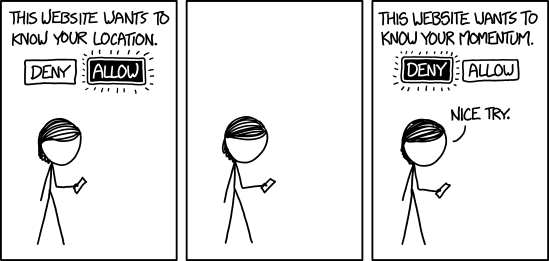
\includegraphics[width=0.8\hsize]{images/xkcd-location-sharing.png}
\caption{XKCD Comic zur Heisenberg Unsch"arfe. Die Benutzerin stellt sicher,
dass die Heisenbergsche Unsch"arferelation nicht verletzt wird. Man kann nicht
sowohl den Ort als auch den Impuls wissen.
\label{skript:heisenberg:xkcd}}
\end{figure}
Im Kapitel~\ref{chapter:drehimpuls} werden wir ein weiteres Paar
von Operatoren wie Ort und Impuls kennen lernen.
Dort untersuchen wir die Komponente $L_3$ des Drehimpulses in $z$-Richtung.
Die dazugeh"orige Ortskoordinaten ist in Kugelkoordinaten die geographische 
L"ange $\varphi$ des Teilchens, welche durch eine Observable mit Operator
$\Phi$ festgestellt werden kann.
In Kugelkoordinaten hat $L_3$ die Form
\[
L_3=\frac{\hbar}{i}\frac{\partial}{\partial\varphi}.
\]
Die Vertauschungsrelationen f"ur $\Phi$ und $L_3$ sind
\[
[\Phi,L_3]=\frac{\hbar}{i}\operatorname{id},
\]
das entspricht den Vertauschungsrelationen von $X$ und $P$.
Zu $\Phi$ und $L_3$ geh"ort nach Satz~\ref{skript:robertson-schroedinger-unschaerfe}
die Unsch"arferelation
\[
\Delta\varphi\cdot\Delta l_3 \ge \frac{\hbar}2,
\]
man kann also den Drehimpuls und die Richtung $\varphi$ nicht gleichzeitig
beliebig genau kennen.
Dies erkl"art den Mouse-Over-Text des Comics in
Abbildung~\ref{skript:heisenberg:xkcd}:
\begin{quote}
Our phones must have great angular momentum sensors because
the compasses really suck.
\end{quote}

\subsection{Unsch"arfe von Energie und Zeit}
In unserem Formalismus hat die Zeit-Koordinate eine ausgezeichnete
Bedeutung, die Schr"odingergleichung beschreibt die Entwicklung
der Zust"ande in der Ortsdarstellung.
Dies hat zur Folge, das wir eine Unsch"arferelation zwischen Energie
und Zeit nicht aus der Robertson-Schr"odinger-Unsch"arferelation
(\ref{skript:uncertainty}) herleiten k"onnen.

Dazu br"auchten wir eine Theorie, welche Orts- und Zeitkoordinaten
gleichwertig behandelt.
Eine solche Theorie ist die spezielle Relativit"atstheorie, welche
zeigt, wie Raum und Zeit untrennbar in einer vierdimensionalen
Raumzeit miteinander verbunden sind.

F"ur einen Spezialfall kann man eine Unsch"arferelation zwischen
Energie und Zeit finden.
Betrachten wir dazu ein Photon mit Energie $E=h\nu$.
Schon die klassische Elektrodynamik erkl"art das Ph"anomen des
Strahlungsdrucks, welches auch schon von Raumfahrzeugen ausgenutzt
werden ist, um durch das Sonnensystem zu `segeln'.
Strahlungsdruck bedeutet, dass Photonen Impuls $p=E/c$ transportieren
und "ubertragen.
Da alle Photonen gleich schnell sind, n"amlich $c$, ist die
Positionsunsch"arfe $\Delta x$ eines Photons im Wesentlichen die
Zeitunsch"arfe der Messung $\Delta t$.
Die Heisenbergsche Unsch"arferelation wird daher
\[
\frac{\hbar}2\le \Delta x\cdot\Delta p=c\Delta t\cdot \frac{\Delta E}{c}=
\Delta t\cdot \Delta E.
\]
Die Unsch"arfe zwischen Zeit und Energie bedeutet, dass die
Energieerhaltung um den Betrag $\Delta E$ verletzt werden darf,
wenn auch nur f"ur kurze Zeit $\Delta t$.

\section*{"Ubungsaufgaben}
\rhead{"Ubungsaufgaben}
\begin{uebungsaufgaben}
\item
\input uebungsaufgaben/07001.tex
\item
\input uebungsaufgaben/07002.tex
\item
\input uebungsaufgaben/07003.tex
\end{uebungsaufgaben}

\chapter{Harmonischer Oszillator\label{chapter:harmonischeroszillator}}
\lhead{Harmonischer Oszillator}
\rhead{}
Das klassische Federpendel ist eines der einfachsten mechanischen 
Systeme. Es ist nicht nur von theoretischer Bedeutung, denn sehr
viele schwingende Systeme k"onnen mit dem gleichen Modell
oder als eine Zusammensetzung solcher einfacher Oszillatoren
beschrieben werden.

In der Quantenmechanik ist die Bedeutung der quantisierten Version
dieses einfachen Systems nicht geringer. Viele Systeme k"onnen
n"aherungsweise durch einen harmonischen Oszillator beschrieben
werden, zum Beispiel die Schwingungen von einfachen Molek"ulen.

Der quantenmechanische harmonische Oszillator hat aber eine Eigenschaft,
die der klassische Oszillator nicht hat: seine Energie ist nicht
kontinuierlich, nur eine diskrete Menge von Energieniveaus sind
m"oglich. Dies ist zwar nicht "uberraschend nach den bisher studierten
Beispielen, doch werden wir hier die mathemtische Technik  der
Auf- und Absteige-Opertoren kennen lernen, mit der die Energieniveaus
und auch die Zustandsvektoren leicht berechnet werden k"onnen.

In der Anwendung auf die Schwingungen einfacher Molek"ule
bedeutet das diskrete Spektrum, dass solche Molek"ule Energie nur in
fest definierten Paketen aufnehmen k"onnen.
Jedes Molek"ul hat also eine charakteristische Menge von Wellenl"angen
von typischerweise infrarotem Licht, welche es absorbieren kann.
Tats"achlich stellt die Infrarotsprektroskopie eine wichtige
Technik in der Chemie dar, mit der Molek"ule identifiziert werden k"onnen.
Wenn ein Molek"ul nur bestimmte Energiepakete aufnehmen kann, dann
wird die W"armekapazit"at ebenfalls temperaturabh"angig sein, und
mit charakteristischen Spr"ungen ansteigen, welche der Anregung
von h"oherenergetischen Molek"ulschwingungen entsprechen.

\section{Der klassische Oszillator}
\rhead{Klasischer Oszillator}
Ein Federpendel ist eine Masse $m$, welches sich unter dem Einfluss
einer Feder mit Federkonstante $K$ bewegt. Ist $x$ die Auslenkung
der Masse aus der Ruhelage, dann "ubt die Feder eine Kraft $-Kx$ 
auf die Masse aus. Die potentielle Energie bei der Auslenkun
$x$ ist daher:
\[
V(x)=\int_0^xK\xi\,d\xi=\frac12Kx^2.
\]
Die Hamilton-Funktion ist daher
\[
H(p,x)=\frac1{2m}p^2+\frac12Kx^2.
\]
Zur Kontrolle leiten wir mit Hilfe der Hamiltonschen Gleichungen
die Bewegungsgleichungen ab:
\begin{align*}
\frac{\partial H}{\partial x}&=Kx
&
&\Rightarrow&
\dot p&=-\frac{\partial H}{\partial x}=-Kx
\\
\frac{\partial H}{\partial p}&=\frac{p}{m}
&
&\Rightarrow&
\dot x&=\frac{\partial H}{\partial p}=\frac{p}{m}.
\end{align*}
Wir erhalten also die klassischen  Bewegungsgleichungen eines harmonischen
Oszillators. 

Die L"osungen dieser Bewegungsgleichungen sind Schwingungen mit 
Frequenz
\[
\omega = \sqrt{\frac{K}{m}},
\]
statt der Konstanten $K$ k"onnten wir auch $K=m\omega^2$ verwenden,
die Hamilton-Funktion ist dann
\begin{equation}
H=\frac1{2m}p^2+\frac12m\omega^2x^2.
\end{equation}

\section{Quantisierung}
\rhead{Quantisierung}
Die Quantisierungsregeln verlangen wieder, dass die Impuls-Variable
durch
\[
p\rightarrow\frac{\hbar}{i}\frac{\partial}{\partial x}
\]
ersetzt wird. Der Hamilton-Operator ist also
\begin{equation}
\hat H
=
-\frac{\hbar^2}{2m}
\frac{\partial^2}{\partial x^2}
+\frac12m\omega^2x^2.
\label{harmoszhamilton}
\end{equation}

Wir suchen jetzt Eigenfunktionen des Hamilton-Operators (\ref{harmoszhamilton}),
also Funktionen $\psi(x)$ und Konstanten $E$ so, dass
\[
\hat H\psi=E\psi.
\]
Da in diesem Problem nur eine einzige Variable auftritt, ist dies ein
Problem "uber gew"ohnliche Differentialgleichungen:
\begin{equation}
-\frac{\hbar^2}{2m} \psi''(x)+\frac12m\omega^2x^2\psi(x)=E\psi(x).
\label{harmoszgleichung}
\end{equation}
In dieser Form ist das Problem etwas umst"andlich zu l"osen.
Wir verwenden statt $x$ die Variablen 
\[
q=\sqrt{\frac{m\omega}{\hbar}}x.
\]
Nennen wir die Funktion $u(q)=\psi(x)$, dann gilt
\begin{align*}
\frac{d}{dq}u(q)&=\frac{d\psi(x)}{dx}\frac{dx}{dq}
=\psi'(x)\sqrt{\frac{\hbar}{m\omega}}
&
\psi'(x)&=\sqrt{\frac{m\omega}{\hbar}}u'(q)
\\
\frac{d^2}{dq^2}u(q)&=\psi''(x)\frac{\hbar}{m\omega}
&
\psi''(x)&=\frac{m\omega}{\hbar}u''(q).
\end{align*}
Setzen wir dies in die Differentialgleichung (\ref{harmoszgleichung})
ein, erhalten wir
\begin{equation}
-\frac{\hbar\omega}{2} u''(q)
+\frac12m\omega^2x^2\psi(x)=E\psi(x).
\end{equation}
Teilen wir dies durch $-\hbar\omega/2$, erhalten wir
\begin{align*}
u''(q) -\frac{m\omega}{\hbar}x^2u(q)=-\frac{2E}{\hbar\omega}u(q),
\end{align*}
oder mit den Abk"urzungen
\[
q=\sqrt{\frac{m\omega}{\hbar}}x
\quad\text{und}\quad
\varepsilon=\frac{E}{\hbar \omega}
\]
die endg"ultige Form der Differentialgleichung
\begin{equation}
u''(q)+(2\varepsilon-q^2) u(q)=0.
\label{harmq}
\end{equation}

\section{Wellenfunktionen}
\rhead{L"osungen}
In diesem Abschnitt l"osen wir die Differentialgleichung (\ref{harmq}).
\subsection{Grundzustand\label{hogrundzustand}}
Da das Potential f"ur grosse Werte von $q$ beliebig gross wird,
muss die Wellenfunktion $u(q)$ f"ur grosse Werte von $q$ exponentiell
schnell abfallen.
Wir versuchen daher einen Ansatz in der Form $u_0(q)=e^{-\alpha q^2}$.
Die Ableitungen von
$u_0(x)$ sind
\begin{align*}
u_0'(q)&=-2\alpha qe^{-\alpha q^2}\\
u_0''(q)&=-2\alpha e^{-\alpha q^2}+4\alpha^2q^2e^{-\alpha q^2}.
\end{align*}
Einsetzen in (\ref{harmoszgleichung})  liefert
\begin{align*}
(-2\alpha e^{-\alpha q^2}+4\alpha^2q^2e^{-\alpha q^2})
+
(2\varepsilon - q^2)e^{-\alpha q^2}&=0
\\
\Leftrightarrow\qquad
\biggl(
-2\alpha +4\alpha^2q^2
+
2\varepsilon - q^2
\biggr)e^{-\alpha q^2}
&=0
\end{align*}
Die letzte Gleichung kann nur erf"ullt werden, wenn der grosse Klammerausdruck
verschwindet, wenn also gilt
\begin{align*}
-2\alpha +4\alpha^2q^2
+
2\varepsilon - q^2
&=0
\\
\Leftrightarrow\qquad
(2\varepsilon-2\alpha)
+
(4\alpha^2-1)q^2
&=0
\end{align*}
Diese Gleichung muss f"ur alle $x$ gelten, die Klammerausdr"ucke
m"ussen also beide verschwinden:
\begin{align*}
(4\alpha^2-1)q^2&=0
&
\alpha&=\frac12
\\
\varepsilon-\alpha&=0
&
\varepsilon&=\frac12.
\end{align*}
Es gibt also tats"achlich eine L"osung, sie muss von der Form
\[
u_0(q)=e^{-\frac{q^2}2}
\]
sein. Der zugeh"orige Eigenwert ist $\varepsilon_0=\frac12$.

In den urspr"unglichen Koordinaten ist der Grundzustand also
\begin{equation}
\psi_0(x)=u_0\biggl(\sqrt{\frac{m\omega}{\hbar}}\biggr)
=
e^{-\frac{m\omega}{2\hbar}}.
\label{grundzustandwellenfunktion}
\end{equation}

% XXX Normierung dieser L"osung
\subsection{Angeregte Zust"ande}
Wir versuchen weitere L"osungen in der Form $u_n(q)=h_n(q)e^{-\frac{q^2}2}$
zu finden, wobei $h_n(q)$ ein Polynom $n$-ten Grades ist.
Wir brauchen wieder die Ableitungen:
\begin{align*}
u'(q)
&=
\bigl(h_n'(q)- qh_n(q)\bigr)e^{-\frac{q^2}2}
\\
u''(q)
&=
\bigl(
h_n''(q)- qh_n'(q)
- h_n(q)
- q h_n'(q)
+q^2h_n(q)
\bigr)e^{-\frac{q^2}2}
\\
&=
\bigl(
h_n''(x)-2 qh_n'(q)
+(q^2-1)h_n(q)
\bigr)e^{-\frac{q^2}2}
\end{align*}
Eingesetzt in die Differentialgleichung erhalten wir
\begin{align}
\bigl(
h_n''(x)-2 qh_n'(q)
+(q^2-1)h_n(q)
\bigr)e^{-\frac{q^2}2}
+(\varepsilon-q^2)h_n(q)e^{-\frac{q^2}2}&=0
\notag
\\
\Leftrightarrow\qquad
h_n''(x)-2 qh_n'(q)
+(\varepsilon - 1)h_n(q)&=0
\label{hermiteequation}
\end{align}
\begin{figure}
\centering
\includegraphics[width=\hsize]{graphics/harmonisch-1.pdf}
\caption{Wellenfunktionen des harmonischen Oszillators
\label{harmonisch-wellenfunktionen}}
\end{figure}
Die Gleichung (\ref{hermiteequation}) heisst auch die 
Hermitesche Differentialgleichung.
Die Funktionen $h_n(q)$ heissen die Hermiteschen Polynome.
Man kann zeigen, dass $\varepsilon=n+\frac12$ sein muss.
Wir werden die Polynome hier nicht ausrechnen, da die Technik der
Auf- und Absteigeoperatoren eine einfachere Methode hierf"ur liefern
wird.
Aus dieser Technik werden sich die Energieniveaus ebenfalls ergeben.
In Abbildung~\ref{harmonisch-wellenfunktionen} sind die Wellenfunktionen
des harmonischen Oszillators f"ur die Energieniveaus bis $n=7$ dargestellt.
Man beachte, dass wir beim Potentialtopf in
Abschnitt~\ref{subsection:potentialtopf} das sich Teilchen mit positiver
Wahrscheinlichkeit in einem Bereich aufhalten kann, der mit der Energie
des Teilchens klassisch verboten ist.
In diesem Bereich f"allt die Aufenthaltswarhscheinlichkeit jedoch
"ahnlich wie beim Potentialtopf exponentiell schnell ab.

\section{Algebraische Eigenschaften}
\rhead{Algebra}
Um die Berechnung der Energieniveaus des harmonischen Oszillators
vorzubereiten wechseln wir zun"achst von den kanoninschen Koordinaten
$x$ und $p$ zu dimensionslosen Gr"ossen $Q$ und $P$, und berechnen
deren algebraischen Eigenschaften.
\subsection{Dimensionslose Operatoren}
Dazu gehen wir zur"uck zum Hamilton-Operator
\[
\hat H=-\frac{\hbar^2}{2m}\frac{\partial^2}{\partial x^2}
+\frac12m\omega^2 x^2
\]
und schreiben ihn unter Verwendung der Operatoren
\[
P=\frac{1}{\sqrt{\hbar m\omega}}p 
\qquad
\text{und}
\qquad
Q=\sqrt{\frac{m\omega}{\hbar}}x
\]
Man kann nachrechnen, dass 
\[
\frac12(P^2+Q^2)
=
\frac{1}{2\hbar m \omega}p^2
+
\frac{m\omega}{2\hbar}x^2
=
-\frac{\hbar}{2 m \omega}\frac{\partial^2}{\partial x^2}
+
\frac{m\omega}{2\hbar}x^2
=\frac{\hat H}{\hbar\omega}
=:\hat{\cal H}
\]
Wir haben den Hamiltonoperator also umgeschrieben mit neuen Operatoren 
$P$ und $Q$.

\subsection{Vertauschungsrelationen}
Wir sollten uns davon "uberzeugen, dass die Operatoren $P$ und $Q$ 
mit den urspr"unglichen $p$ und $x$ vergleichbar sind, und berechnen
daher die Vertauschungsrelationen:
\begin{align*}
[P,Q]
&=
\frac{1}{\sqrt{\hbar m\omega}} \sqrt{\frac{m\omega}{\hbar}}[p, x]
=
\frac1{\hbar}[p,x]
\end{align*}
Wir erinnern an die Vertauschungsrelationen f"ur die Operatoren $p$ und $x$:
\begin{align*}
\left[\frac{\hbar}{i}\frac{\partial}{\partial x}, x\right]\psi(x)
&=
\frac{\hbar}{i}\frac{\partial}{\partial x}(x\psi(x))
-x\frac{\hbar}{i}\frac{\partial}{\partial x}\psi(x)
=
\frac{\hbar}{i}\psi(x)
x\frac{\hbar}{i}\frac{\partial \psi(x)}{\partial x}
-x\frac{\hbar}{i}\frac{\partial}{\partial x}\psi(x)
=\frac{\hbar}{i}\psi(x)
\\
[p,x]&=\frac{\hbar}{i}\operatorname{id}.
\end{align*}
Damit sind jetzt auch die Vertauschungsoperatoren f"ur $P$ und $Q$ 
bekannt:
\[
[P,Q]=\frac1{i}\operatorname{id}=-i\operatorname{id}.
\]

\section{Auf- und Absteigeoperatoren}
\rhead{Auf- und Absteigeoperatoren}
Die Methode der Auf- und Absteige-Operatoren erlaubt, die Eigenwerte
und Eigenvektoren direkt aus dem Grundzustand zu ermitteln.
Wir sehen Sie hier in einem einfachen Spezialfall am Werk.
Sie l"asst sich aber verallgemeinern, man kann damit zum Beispiel
auch den Drehimpuls verstehen (Kapitel~\ref{chapter:drehimpuls}).
Ja die Methode hat sogar g"anzlich von der Quantenmechanik unabh"angige
Anwendungen bei der Konstruktion von L"osungen allgemeinerer Randwertprobleme
f"ur gew"ohnliche Differentialgleichung.

\subsection{Definition}
Wir definieren jetzt die Operatoren
\[
a=\frac1{\sqrt{2}}(Q+iP)
\qquad\text{und}\qquad
a^+=\frac1{\sqrt{2}}(Q-iP).
\]
Zun"achst ist klar, dass $a$ und $a^+$ nicht selbstadjungiert sind,
vielmehr ist
\[
a^*=\frac1{\sqrt{2}}(Q^*-iP^*)=\frac1{\sqrt{2}}(Q-iP)=a^+.
\]
Damit entsprechen die Operatoren $a$ und $a^+$ nicht einer physikalisch
messbaren Gr"osse. 

Unser Ziel ist die Berechnung der Eigenwerte und Eigenvektoren
des harmonischen Oszillators mit algebraischen Mitteln. Dazu brauchen
wir die algebraischen Eigenschaften der Operatoren $a$ und $a^+$,
insbesondere deren Produkte und Vertauschungsrelationen.
\begin{align*}
aa^+
&=
\frac1{\sqrt{2}}(Q+iP)\frac1{\sqrt{2}}(Q-iP)
=
\frac12(Q^2+P^2+i[P,Q])
=
\hat{\cal H}+\frac12
\\
a^+a
&=
\frac1{\sqrt{2}}(Q-iP)\frac1{\sqrt{2}}(Q+iP)
=
\frac12(Q^2+P^2+i[Q,P])
=
\hat{\cal H}-\frac12=:N
\end{align*}
Daraus folgt auch
\[
[a,a^+]=\operatorname{id},
\]
und die weiteren Vertauschungsrelationen
\begin{align*}
[N,a^+]
&=a^+aa^+-aa^+a^+=[a,a^+]a^+=a^+
&
[N,a]
&=a^+aa-aa^+a=[a^+,a]a=-a
\\
&=[\hat{\cal H},a^+]
&
&=[\hat{\cal H}, a].
\end{align*}

\subsection{Wirkung auf Zustandsvektoren}
Nehmen wir an, $|n\rangle$ sei der $n$-te Eigenvektor von $\hat{\cal H}$,
mit Energie $\varepsilon_n$, also
\[
\hat{\cal H}|n\rangle = \varepsilon_n|n\rangle.
\]
Wenden wir die Operatoren $a$ und $a^+$ auf $|n\rangle$ anwenden, erhalten
wir einen neuen Eigenvektor:
\begin{align*}
\hat{\cal H}a^+\,|n\rangle
&=
([\hat{\cal H}, a^+] + a^+\hat{\cal H})\,|n\rangle
=
(1 + \varepsilon_n)a^+\,|n\rangle
\\
\hat{\cal H}a\,|n\rangle
&=
([\hat{\cal H}, a] + a\hat{\cal H})\,|n\rangle
=
(\varepsilon_n - 1)a\,|n\rangle
\end{align*}
Insbesondere ist $a^+\,|n\rangle$ ein Eigenvektor mit Energie
$E_n+1$, und $a|n\rangle$ ein Eigenvektor mit Energie $\varepsilon_n-1$.
Man kann also mit dem Operator $a^+$ zu Zust"anden h"oherer Energie
aufsteigen, und mit $a$ zu Zust"anden niedrigerer Energie absteigen.

Beim Auf- und Absteigen bleibt die Normierung aber nicht notwendigerweise
erhalten, wir k"onnen also nicht davon ausgehen, dass $a^+|n\rangle$
wieder ein normierter Eigenvektor ist.
Um die Norm zu korrigieren, berechen wir die Norm des neuen Vektors:
\[
(a^+\langle n|) a^+\,|n\rangle
=
\langle n|\,aa^+\,|n\rangle
=
\langle n|\,\hat{\cal H}+{\textstyle\frac12}\,|n\rangle
=
(\varepsilon_n+{\textstyle\frac12})\langle n|n\rangle
=
\varepsilon_n+\textstyle\frac12
\]
Wenn man also durch Aufsteigen wieder einen normierten Zustandsvektor
erhalten will, muss man den erhaltenen Vektor renormieren:
\begin{equation}
|n+1\rangle = \frac1{\sqrt{\varepsilon_n+\textstyle\frac12}}|n\rangle.
\label{aufsteigrenormierung}
\end{equation}

\subsection{Eigenwerte und Zustandsvektoren}
Die Energie eines harmonischen Operators ist immer positiv,
also kann man mit $a$ nicht beliebig lange absteigen. Es muss einen
Zustand $|0\rangle$ kleinster Energie geben. M"ochte man weiter
absteigen, darf kein Zustandsvektor mehr entstehen, es muss also
$a|0\rangle=0$ sein. Durch Multiplikation mit $a^+$ folgt
\[
0=a^+a|0\rangle=(\hat{\cal H}-\textstyle\frac12)\,|0\rangle
\quad
\Rightarrow
\quad
\hat{\cal H}\,|0\rangle=\frac12\,|0\rangle
\quad
\Rightarrow
\quad
\varepsilon_0=\frac12.
\]
Der Grundzustand hat also immer den Eigenwert $\frac12$, oder die
Energie $\frac12\hbar\omega$. Diesen Wert haben wir auch schon in
Abschnitt~\ref{hogrundzustand} erhalten.
Die angeregten Zust"ande haben Energie
\[
E_n
=
\hbar\omega\biggl(n+\frac12\biggr),
\]
wobei $n\ge 0$ eine nat"urliche Zahl sein muss.

Beim Aufsteigen ver"andert sich jeweils die Normierung.
Will man die Energieeigenzust"ande so konstruieren, muss man nach jedem
Aufsteigeschritt die Normierung mit Hilfe von (\ref{aufsteigrenormierung})
korrigieren. Dabei kann man verwenden, dass $\varepsilon_n = n+\frac12$
ist. Nach $n$-maligem Aufsteigen aus dem Grundzustand hat man die
Norm um den Faktor
\begin{align}
N_n
&=
\frac12\cdot\biggl(1+\frac12\biggr)\cdot\biggl(2+\frac12\biggr)\cdot\ldots\cdot
\biggl(n+\frac12\biggr)
=
\frac12\cdot\frac32\cdot\frac52\cdot\ldots\cdot\frac{2n+1}2
\notag
\\
&=
\frac1{2^n}
\frac{1\cdot 2\cdot 3\cdot 4\cdot 5\cdot \ldots \cdot (2n+1)\cdot 2n}%
{2\cdot 4\cdot 6\cdot \ldots \cdot 2n}
=\frac1{2^{2n}}\frac{2n!}{n!}
\label{aufsteigrenormierungn}
\end{align}
ver"andert.

Der Aufsteigeoperator $a^+$ erm"oglicht jetzt auch, aus dem Grundzustand
alle h"oheren Zust"ande konstruieren:
\begin{equation}
|n\rangle
=
\frac{1}{\sqrt{N_n}}(a^+)^n\,|0\rangle
=
2^n \sqrt{\frac{n!}{2n!}} (a^+)^n\,|0\rangle,
\end{equation}
wobei $N_n$ der Normierungsfaktor aus (\ref{aufsteigrenormierungn}) ist.

Da wir den Grundzustand bereits aus Abschnitt~\ref{hogrundzustand} kennen,
k"onnen wir die Wellenfunktionen f"ur die h"oheren Zust"ande berechnen,
indem wir den Operator $a^+$ wieder in den urspr"unglichen Koordinaten
ausdr"ucken:
\begin{equation}
a^+=\frac1{\sqrt{2}}(Q+iP)
=
\frac1{\sqrt{2}}\biggl(
\sqrt{\frac{m\omega}{\hbar}}x
+i
\frac{1}{\sqrt{\hbar m\omega}}\frac{\hbar}{i}\frac{\partial}{\partial x}
\biggr)
=
\frac1{\sqrt{2}}
\biggl(
\sqrt{\frac{m\omega}{\hbar}}x
+
\sqrt{\frac{\hbar}{m\omega}}\frac{\partial}{\partial x}
\biggr)
\label{aufsteigeho}
\end{equation}
Die Wellenfunktionen des Zustands $|n\rangle$ erh"alt man also, indem
man den Operator $a^+$ in der Form \ref{aufsteigeho} auf die Wellenfunktion
$\psi_0$ wie in (\ref{grundzustandwellenfunktion}) anwendet.

Wir fassen die Resultate "uber den harmonischen Oszillator in einem Satz
zusammen:
\begin{satz}
Ein harmonischer Oszillator mit Hamilton-Operator
\[
\frac{1}{2m}p^2+\frac{m}{2}\omega^2x^2
=
-\frac{\hbar^2}{2m}\frac{\partial^2}{\partial x^2}
+\frac{m}2\omega^2x^2
\]
hat Eigenzust"ande mit Energie
\begin{equation}
E_n
=
\hbar\omega\biggl(n+\frac12\biggr),
\label{hoenergieniveaus}
\end{equation}
die Eigenzust"ande k"onnen durch Anwendung des Aufsteigeoperators $a^+$
aus (\ref{aufsteigeho}) auf die Wellenfunktion des Grundzustandes
$\psi(x)=e^{-\frac{m\omega}{2\hbar}x^2}$
mit geeigneter Normierung.
\end{satz}

\section{"Ubungsaufgaben}
\begin{uebungsaufgaben}
\item
\input uebungsaufgaben/08001.tex
\item
\input uebungsaufgaben/08002.tex
\end{uebungsaufgaben}

\chapter{Wasserstoffatom\label{chapter:wasserstoff}}
\lhead{Wasserstoffatom}
\rhead{}
Der bisher entwickelte Formalismus erlaubt bereits, das Wasserstoff-Atom
zu verstehen. Die Quantenmechanik erkl"art die Stabilit"at der
Materie, und sagt das Wasserstoff-Spektrum korrekt voraus.
\section{Schr"odinger-Gleichung f"ur das Wasserstoffatom}
\rhead{Schr"odingergleichung f"ur das Wasserstoffatom}
Die Hamilton-Funktion eines Elektrons im Potential eines einzelnen
Protons, welches sich im Nullpunkt des Koordinatensystems befindet,
ist
\begin{equation}
H=\frac1{2m_e}p^2 + V(r)
=\frac1{2m_e}p^2 - \frac1{4\pi\varepsilon_0}\frac{e^2}{r}.
\label{skript:h2hamilton}
\end{equation}
Darin ist $m_e$ die Masse des Elektrons, $e$ ist die Elementarladung.
$r$ ist die Entfernung eines Punktes vom Nullpunkt.
Der Impuls ist als Vektor zu verstehen, also $p^2=p_x^2+p_y^2+p_z^2$.

Wir suchen eine L"osung des quantisierten Systems mit Zustandsvektoren, die von
den Ortskoordinaten abh"angen.
Nach den Quantisierungsregeln m"ussen die Impulse in der Hamiltonfunktion
durch Ableitungsoperatoren
\begin{equation}
p_x\rightarrow \frac{\hbar}{i}\frac{\partial}{\partial x},
\qquad
p_y\rightarrow \frac{\hbar}{i}\frac{\partial}{\partial y},
\quad
\text{und}
\quad
p_y\rightarrow \frac{\hbar}{i}\frac{\partial}{\partial z}.
\label{skript:h2quant}
\end{equation}
ersetzt werden. Wendet man die Ersetzungen (\ref{skript:h2quant}) auf die
Hamilton-Funktion (\ref{skript:h2hamilton}) an, erh"alt man den Hamilton-Operator
f"ur das Wasserstoff-Atom:
\[
\hat H=-\frac{\hbar^2}{2m_e}\biggl(
\frac{\partial^2}{\partial x^2}+
\frac{\partial^2}{\partial y^2}+
\frac{\partial^2}{\partial z^2}
\biggr)-\frac1{4\pi\varepsilon_0}\frac{e^2}{r}
=-\frac{\hbar^2}{2m_e}\Delta -\frac1{4\pi\varepsilon_0}\frac{e^2}{r}.
\]
Wir suchen zeitunabh"angige Zust"ande, also Eigenfunktionen dieses
Operators. Wir erwarten eine Menge von Zustandsvektoren $|\psi\rangle$
mit zugeh"origen Eigenwerten $E$, so dass
\begin{equation}
\hat H\,|\psi\rangle = E\,|\psi\rangle.
\label{skript:h2schroedinger}
\end{equation}
(\ref{skript:h2schroedinger}) ist eine partielle Differentialgleichung.
Wir beabsichtigen nicht, eine allgemeine Theorie der partiellen
Differentialgleichungen zu entwickeln.
F"ur unsere Zwecke reicht es, eine ad hoc L"osung zu finden.

\section{Kugelkoordinaten}
\rhead{Kugelkoordinaten}
Das Eigenwertproblem (\ref{skript:h2schroedinger}) kann in kartesischen Koordinaten
nicht direkt gel"ost werden. Dies liegt daran, dass die kartesischen
Koordinaten die vorhandene Kugelsymmetrie des Problems nicht ausreichend
ber"ucksichtigen. Es ist viel besser, Kugelkoordinaten zu verwenden.

Die Umrechnungn zwischen Kugelkoordinaten $(r,\vartheta,\varphi)$ und
kartesischen Koordinaten $(x,y,z)$ ist gegeben durch
\begin{align*}
x&=r
\sin\vartheta
\cos\varphi
\\
y&=r
\sin\vartheta
\sin\varphi
\\
z&=r\cos \vartheta
\end{align*}
Eine etwas m"uhsame Rechnung erlaubt, den Laplace-Operator in Kugelkoordinaten
auszudr"ucken:
\[
\Delta
=
\frac1{r^2}\frac{\partial}{\partial r}\biggl(
r^2\frac{\partial}{\partial r}
\biggr)
+\frac1{r^2\sin\vartheta}\frac{\partial}{\partial \vartheta}\biggl(
 \sin\vartheta \frac{\partial}{\partial\vartheta}
\biggr)
+
\frac1{r^2\sin^2\vartheta}\frac{\partial^2}{\partial\varphi^2}.
\]

\section{L"osung der Schr"odingergleichung}
\rhead{L"osung der Schr"odingergleichung}
Wir suchen jetzt also L"osungen des Eigenwertproblems (\ref{skript:h2schroedinger})
als $L^2$-Funktionen in Kugel-Koordinaten $(r,\varphi,\vartheta)$. Wir
verwenden dazu die Methode der Separation der Variablen.

\subsection{Separationsansatz}
Wir nehmen an,
dass sich die L"osung $\psi(r,\vartheta,\varphi)$ schreiben l"asst als
ein Produkt von drei Funktionen, die je nur von einer Koordinate
abh"angen. Wir setzen also an
\begin{equation}
\psi(r,\vartheta,\varphi)=R(r)\cdot
\Theta(\vartheta)\cdot
\Phi(\varphi)
\label{skript:sepansatz}
\end{equation}
und setzen dies in das Eigenwertproblem ein. Dazu brauchen wir die Ableitung
nach $r$, $\varphi$ und $\vartheta$ von $\psi(r,\varphi,\vartheta)$, doch
diese Ableitungen wirken jeweils nur auf einen der Faktoren:
\[
\frac{\partial}{\partial r}\psi(r,\vartheta,\varphi)
=
\frac{\partial R(r)}{\partial r}
\cdot \Theta(\vartheta)
\cdot  \Phi(\varphi)
+
R(r)
\cdot \Theta(\vartheta)
\cdot \underbrace{\frac{\partial\Phi(\varphi)}{\partial\varphi}}_{=0}
+
R(r)
\cdot \underbrace{\frac{\partial \Theta(\vartheta)}{\partial\vartheta}}_{=0}
\cdot \Phi(\varphi)
=
R'(r)
\cdot \Theta(\vartheta),
\cdot \Phi(\varphi)
\]
und analog f"ur die anderen Variablen.
Wir k"onnen also so tun, als ob die Ableitungen jeweils nur auf genau
einen der Faktoren wirken.
\begin{equation}
\Delta \psi
=
\frac1{r^2}\frac{d}{dr}\bigl(r^2R'(r)\bigr)
\cdot \Theta(\vartheta)
\cdot \Phi(\varphi)
+
R(r)
\cdot \frac{1}{r^2\sin\vartheta}
\frac{d}{d\vartheta}(\sin\vartheta \Theta'(\vartheta))
\cdot \Phi(\varphi)
+
\frac{R(r)}{r^2\sin^2\vartheta}
\cdot \Theta(\vartheta)
\cdot \Phi''(\varphi)
\label{skript:separated}
\end{equation}
Man beachte, dass in allen Termen immer nur einer der Faktoren des
Separationsansatzes abgeleitet wurde.

Das Eigenwertproblem, welches zu l"osen ist, wird jetzt in Kugelkoordinaten
zu
\[
-\frac{\hbar^2}{2m_e} \Delta\psi(r,\vartheta,\varphi)
-\frac{1}{4\pi\varepsilon_0}\frac{e^2}{r}\psi(r,\vartheta,\varphi)
=E\psi(r,\vartheta,\varphi).
\]

\subsection{Separation von $\varphi$}
Keine der drei Faktoren des Ansatzes (\ref{skript:sepansatz}) f"ur
$\psi(r,\vartheta,\varphi)$ kann verschwinden, sonst erhielten wir die 
Nullfunktion, also nicht einen Eigenvektor von $\hat H$.
Nat"urlich k"onnen die Faktoren einzelne Nullstellen haben, aber ausserhalb
dieser Nullstellen kann man die Gleichung (\ref{skript:separated}) durch 
$\psi(r,\vartheta,\varphi)$ teilen. Wir erhalten
\begin{equation*}
-\frac{\hbar^2}{2m_e}\biggl(
\frac{1}{R(r)}
\frac{1}{r^2}
\frac{d}{dr}(r^2R'(r))
+
\frac{1}{\Theta(\vartheta) r^2\sin\vartheta}\frac{d}{d\vartheta}(\sin\vartheta \Theta'(\vartheta))
+
\frac{1}{r^2\sin^2\vartheta}\frac{\Phi''(\varphi)}{\Phi(\varphi)}
\biggr)
-\frac1{4\pi\varepsilon_0}\frac{e^2}{r}
=
E.
\end{equation*}
Bringen wir ausserdem alle Terme mit $\varphi$ auf die rechte Seite,
und multiplizieren mit $r^2\sin^2\vartheta$
ergibt sich
\begin{equation*}
-\frac{\hbar^2}{2m_e}
\frac{1}{R(r)}\sin^2\vartheta \frac{d}{dr}(r^2R'(r))
-
\frac{\hbar^2}{2m_e}
\frac{\sin\vartheta}{\Theta(\vartheta) }\frac{d}{d\vartheta}(\sin\vartheta \Theta'(\vartheta))
-\biggl(\frac1{4\pi\varepsilon_0}\frac{e^2}{r}
+
E\biggr)r^2\sin^2\vartheta
=
\frac{\hbar^2}{2m_e}\frac{\Phi''(\varphi)}{\Phi(\varphi)}.
\end{equation*}
Indem wir durch den Faktor $-\hbar^2/2m_e$ dividieren, wir die Gleichung
etwas "ubersichtlicher:
\begin{equation}
\frac{1}{R(r)}\sin^2\vartheta \frac{d}{dr}(r^2R'(r))
+
\frac{\sin\vartheta}{\Theta(\vartheta) }\frac{d}{d\vartheta}(\sin\vartheta \Theta'(\vartheta))
+\biggl(\frac{m_e}{2\pi\varepsilon_0\hbar^2}\frac{e^2}{r}
+
\frac{2m_eE}{\hbar^2}\biggr)r^2\sin^2\vartheta
=
-\frac{\Phi''(\varphi)}{\Phi(\varphi)}.
\label{skript:phisepariert}
\end{equation}
Die linke Seite dieser Gleichung h"angt nicht von $\varphi$ ab, also
darf auch die rechte Seite nicht von $\varphi$ abh"angen, sie muss
eine Konstante sein. Wir nennen die Konstante $m^2$ (dies wird sich
als zweckm"assig herausstellen). Wir haben also aus der urspr"unglichen
partiellen Differentialgleichung eine gew"ohnliche Differentialgleichung
\[
-\frac{\Phi''(\varphi)}{\Phi(\varphi)}=m^2
\quad\Leftrightarrow\quad
\Phi''(\varphi)=-m^2\Phi(\varphi)
\]
f"ur die Funktion $\Phi(\varphi)$ gefunden.
Die L"osungen einer solchen Differentialgleichung zweiter Ordnung sind
wohl bekannt: $e^{im\varphi}$ und $e^{-im\varphi}$. Damit die Funktion
periodisch wird, muss $m$ eine nat"urliche Zahl sein, $m=0,1,2,\dots$.

\subsection{Separation von $r$ und $\vartheta$}
In der Gleichung (\ref{skript:phisepariert}) kommt auf der linken Seite nur
noch $r$ und $\vartheta$ vor.  Die rechte Seite haben wir inzwischen auf
die m"oglichen Werte $m^2$ reduziert. Teilen wir die Gleichung durch
$\sin^2\vartheta$, und bringen die von $\vartheta$ abh"angenden Terme
auf die rechte Seite, erhalten wir die Gleichung
\begin{equation}
\frac{1}{R(r)}\frac{d}{dr}\bigl(r^2R'(r)\bigr)
+\biggl(\frac{m_e}{2\pi\varepsilon_0\hbar^2}\frac{e^2}{r}
+
\frac{2m_eE}{\hbar^2}\biggr)r^2
=
-
\frac1{\sin\vartheta\Theta(\vartheta) }
\frac{d}{d\vartheta}\bigl(\sin\vartheta \Theta'(\vartheta)\bigr)
+
\frac{m^2}{\sin^2\vartheta}
\label{skript:thetasepariert}
\end{equation}
Die linke Seite von (\ref{skript:thetasepariert}) h"angt nicht von $\vartheta$
ab, also kann auch die rechte Seite nicht von $\vartheta$ abh"angen.
Ebenso h"angt die rechte Seite nicht von $r$, also kann auch die linke
nicht von $r$ abh"angen. Beide Seiten m"ussen also konstant sein,
wir nennen die Konstante $\lambda$.

\subsection{Abh"angigkeit von $\vartheta$}
Die Funktion $\Theta(\vartheta)$ auf der rechten Seite ist eigentlich
eine Funktion von $z=\cos\vartheta$. Wir schreiben
$Z(z)=Z(\cos\vartheta)=\Theta(\vartheta)$. Die Ableitung nach $\vartheta$
kann dann umgeschrieben werden in eine Ableitung nach $z$
\begin{align*}
\Theta'(\vartheta)&=
\frac{d}{d\vartheta}Z(z)=Z'(z)\frac{dz}{d\vartheta}=\sin\vartheta Z'(z)
\\
\frac{d}{dz}&=\frac1{\sin\vartheta}\frac{d}{d\vartheta}
\end{align*}
Nat"urlich gilt auch $1-z^2=\sin^2\vartheta$, so dass die rechte Seite
von (\ref{skript:thetasepariert}) zu
\begin{equation}
-
\frac1{\Theta(\vartheta)}
\frac1{\sin\vartheta}
\frac{d}{d\vartheta}\biggl(
\sin^2\vartheta \frac1{\sin\vartheta}\frac{d}{d\vartheta}\Theta'(\vartheta)
\biggr)
+
\frac{m^2}{\sin^2\vartheta}
=
-\frac1{Z(z)}\frac{d}{dz}\biggl(
(1-z^2)\frac{d}{dz}Z(z)
\biggr)
+
\frac{m^2}{1-z^2}
\end{equation}
wird. Dieser Ausdruck muss konstant sein, wir nennen die Konstante 
$\lambda$:
\begin{equation}
-\frac1{Z(z)}\frac{d}{dz}\biggl(
(1-z^2)\frac{d}{dz}Z(z)
\biggr)
+
\frac{m^2}{1-z^2}
=\lambda
\end{equation}
oder
\begin{equation}
\frac{d}{dz}\biggl(
(1-z^2)\frac{d}{dz}Z(z)
\biggr)
+\biggl(\lambda
-
\frac{m^2}{1-z^2}
\biggr)Z(z)
=0
\label{skript:legendregleichung}
\end{equation}

\subsubsection{Spezialfall $m=0$}
Wir untersuchen diese L"osung zun"achst f"ur den Spezialfall $m=0$,
d.~h.~wir m"ussen die Differentialgleichung
\begin{equation}
\frac{d}{dz}\biggl(
(1-z^2)\frac{d}{dz}Z(z)
\biggr)
+\lambda Z(z)=0
\end{equation}
l"osen.
Dies ist die sogenannte Legendresche Differentialgleichung,
deren L"osung in einer guten Formelsammlung gefunden werden k"onnen.

Wir versuchen eine L"osung in Form eines Polynoms vom
Grade $l$, also 
\begin{equation}
P_l(z)=a_0+a_1z+\dots+a_lz^l.
\label{skript:legendreansatz}
\end{equation}
Setzen wir dies in die Gleichung ein, und betrachten nur die
Terme vom Grad $z^l$:
\begin{align*}
\frac{d}{dz}(-z^2la_lz^{l-1})
+
\lambda a_lz^l&=0
\\
-l(l+1)a_lz^l+\lambda a_lz^l&=0,
\end{align*}
Es folgt, dass $\lambda = l(l+1)$ sein muss, wobei $l$ eine ganze
Zahl sein muss.

Wie jede Differentialgleichung zweiter Ordnung hat die Legendresche
Differentialgleichung ausser den $P_l$ auch noch eine L"osung
$Q_l$, diese ist jedoch nicht eschr"ankt und kommt daher als L"osungsfunktion
f"ur unser Problem nicht in Frage.

\subsubsection{Legendre-Polynome}
Indem man den Ansatz (\ref{skript:legendreansatz}) f"ur alle Koeffizienten
auswertet, nicht nur f"ur $a_l$, kann man die Polynome $P_l(z)$ 
bestimmen, sie heissen Legendre-Polynome.
"Uber die Jahre wurde eine umfangreiche Theorie der Legendre-Polynome
aufgebaut, so gilt zum Beispiel die folgende Formel von Rodrigues
\[
P_l(z)=\frac1{2^ll!}\frac{d^l}{dz^l}(z^2 - 1)^l.
\]
Die Legendre-Polynome sind orthogonal.

%Durch Einsetzen in die Differentialgleichung kann man verifizieren,
%dass dies tats"achlich eine L"osung ist:
%\begin{align*}
%\frac{d}{dz}\biggl(
%(1-z^2)\frac{d}{dz}
%\frac1{2^ll!}\frac{d^l}{dz^l}(z^2 - 1)^l.
%\biggr)
%&=
%\frac1{2^ll!}
%\frac{d}{dz}\biggl(
%(1-z^2)
%\frac{d^l}{dz^l}l(z^2 - 1)^{l-1}2z.
%\biggr)
%\\
%&=
%\frac1{2^ll!}
%\biggl(
%(-2z)
%\frac{d^l}{dz^l}l(z^2 - 1)^{l-1}2z.
%+
%(1-z^2)
%\frac{d^l}{dz^l}l\frac{d}{dz}\bigl((z^2 - 1)^{l-1}2z\bigr)
%\biggr)
%\\
%\end{align*}

\subsubsection{Der Fall $m\ne 0$}
F"ur den allgemeinen Fall mit beliebigen $m$ m"ussen L"osungen der
Gleichung
\begin{equation}
\frac{d}{dz}\biggl((1-z^2)\frac{d}{dz}Z(z)\biggr)
+\biggl(\lambda -\frac{m^2}{1-z^2}\biggr)Z(z)=0
\end{equation}
gefunden werden. Man kann zeigen, dass die Funktionen
\[
P_l^m(z)=
(1-z^2)^{\frac{m}2}\frac{d^m}{d^z}P_l(z)
\]
eine L"osung f"ur $\lambda=l(l+1)$ ist.
Auch diese allgemeineren Funktionen $P_l^m(z)$ sind orthogonal.

\subsection{Abh"angigkeit von $r$}
Die Funktion $R(r)$ erf"ullt die Differentialgleichung
\begin{align}
\frac{1}{r^2}\frac{d}{dr}\bigl(r^2R'(r)\bigr)
+\biggl(\frac{m_e}{2\pi\varepsilon_0\hbar^2}\frac{e^2}{r}
+
\frac{2m_eE}{\hbar^2}
-\frac{\lambda}{r^2}
\biggr)R(r)
&=0
\label{skript:radialgleichung}
\end{align}
Wir wissen bereits, dass $\lambda=l(l+1)$, also k"onnen wir die
Gleichung umformen zu
\begin{align*}
\frac{1}{r^2}\frac{d}{dr}\bigl(r^2R'(r)\bigr)
+\biggl(\frac{m_e}{2\pi\varepsilon_0\hbar^2}\frac{e^2}{r}
+
\frac{2m_eE}{\hbar^2}
-\frac{l(l+1)}{r^2}
\biggr)R(r)
&=0.
\end{align*}
Die Gleichungen k"onnen etwas vereinfacht werden, wenn man einen
Faktor $r$ abspaltet, also 
\[
R(r)=\frac{\chi(r)}{r}
\]
verwendet.
Die Ableitungen von $R(r)$ sind
\begin{align*}
R'(r)&=\frac{\chi'(r)r-\chi(r)}{r^2},\\
\frac{d}{dr}\bigl(r^2R'(r)\bigr)
&=
\frac{d}{dr}\bigl(\chi'(r)r-\chi(r)\bigr)
=
\chi''(r)r+\chi'(r)-\chi'(r)=r\chi''(r).
\end{align*}
Setzt man dies in die Differentialgleichung (\ref{skript:radialgleichung}) ein,
erh"alt
\begin{align*}
\frac{\chi''(r)}{r}
+\biggl(\frac{m_e}{2\pi\varepsilon_0\hbar^2}\frac{e^2}{r}
+
\frac{2m_eE}{\hbar^2}
-\frac{l(l+1)}{r^2}
\biggr)\frac{\chi(r)}{r}
&=0
\\
\chi''(r)
+\biggl(\frac{m_e}{2\pi\varepsilon_0\hbar^2}\frac{e^2}{r}
+
\frac{2m_eE}{\hbar^2}
-\frac{l(l+1)}{r^2}
\biggr)\chi(r)
&=0
\end{align*}


Die gesuchte L"osung $R(r)$ muss f"ur grosse Entfernungen $r$ exponentiell
abfallen.
Wir versuchen daher einen Ansatz der Form
\[
R(r)=\biggl(\frac{2r}{n}\biggr)^le^{-\frac{r}{n}}w\biggl(\frac{2r}{n}\biggr)
\]

%Wir versuchen eine L"osung f"ur $R(r)$ zu finden. Um die Differentialgleichung
%f"ur $R(r)$ etwas zu vereinfachen, formulieren wir sie um f"ur 
%\[
%R(r)=\frac{\chi(r)}{r}.
%\]
%Die Ableitung von $R(r)$ ist
%\[
%R'(r)=\frac{\chi'(r)r-\chi(r)}{r^2},
%\]
%Der erste Term in (\ref{skript:thetasepariert}) wird dadurch besonders einfach,
%n"amlich
%\[
%\frac1{r^2}\frac{d}{dr}\bigl(r^2R'(r)\bigr)
%=\frac1{r^2}\frac{d}{dr} \bigl(\chi'(r)r-\chi(r)\bigr)
%=\frac1{r^2}(\chi''(r)r +\chi'(r) -\chi'(r))=\frac{\chi''(r)}r,
%\]
%und die Differentialgleichung wird
%\begin{align*}
%\frac{\chi''(r)}{r}
%+
%\biggl(\frac{m_e}{2\pi\varepsilon_0\hbar^2}\frac{e^2}{r}
%+
%\frac{2m_eE}{\hbar^2}
%-\frac{\lambda}{r^2}
%\biggr)R(r)
%&=0
%\\
%\Rightarrow\qquad
%\chi''(r)
%+
%\biggl(\frac{m_e}{2\pi\varepsilon_0\hbar^2}\frac{e^2}{r}
%+
%\frac{2m_eE}{\hbar^2}
%-\frac{\lambda}{r^2}
%\biggr)\chi(r)
%&=0.
%\end{align*}

\section{Hybridorbitale}

\chapter{St"orungstheorie\label{chapter:stoerungstheorie}}
\lhead{St"orungstheorie}
\rhead{}
Die St"orungstheorie geht davon aus, dass eine Basis von Zust"anden eines
quantenmechanischen Systems bereits bekannt ist. Eine kleine
"Anderung des Systems sollte sich dann in nur kleinen "Anderungen
der Zust"ande und ihrer Energieniveaus "aussern.
Diese Methode kann verwendet werden, um die Ver"anderung der Energieniveaus
eines Atoms zu berechnen, wenn dieses in ein "ausseres elektrisches Feld
oder ein "ausseres Magnetfeld gebracht wird.

\section{Grundprinzip der St"orungstheorie}
\rhead{Grundprinzip}
\index{stoerungstheorie@St\"orungstheorie!Prinzip}
Wir beginnen die Untersuchung mit einer Anwendung auf die Nullstellen
eines quadratischen Polynoms. Sei also
\[
p(x) = ax^2 + bx + c
\]
ein quadratisches Polynom, nat"urlich k"onnen wir sofort die Nullstellen
mit Hilfe der L"osungsformel
\begin{equation}
x_{\pm}=\frac{-b\pm\sqrt{b^2-4ac}}{2a}
\label{skript:mitternachtsformel}
\end{equation}
finden.  Ver"andert man die Koeffizienten von $p(x)$, werden sich auch
die beiden Nullstellen ver"andern, sie k"onnen mit der Formel
(\ref{skript:mitternachtsformel}) bestimmt werden.

Nehmen wir also an, dass die Koeffizienten $a$, $b$ und $c$ von $p(x)$
von einem Parameter $\varepsilon$ abh"angen. Statt der Konstanten verwenden
wir also Funktionen
\begin{align*}
a(\varepsilon)&=a_0+a_1\varepsilon+a_2\varepsilon^2+\dots\\
b(\varepsilon)&=b_0+b_1\varepsilon+b_2\varepsilon^2+\dots\\
c(\varepsilon)&=c_0+c_1\varepsilon+c_2\varepsilon^2+\dots
\end{align*}
von $\varepsilon$. Mit diesen Koeffizienten wird aus dem Polynom $p(x)$
eine Familie von Polynomen
\[
p_\varepsilon(x)=a(\varepsilon)x^2 + b(\varepsilon)x+c(\varepsilon).
\]
Die L"osungsformel (\ref{skript:mitternachtsformel}) liefert weiterhin die
Nullstellen von $p_{\varepsilon}(x)=0$.
Sei $x_0$ eine der Nullstellen von $p_0(x) = 0$.

Statt die L"osungen von $p_{\varepsilon}(x)=0$ mit Hilfe der L"osungsformel
zu finden, k"onnen wir auch versuchen, von $x_0$ ausgehend eine N"aherung
zu finden. Diese L"osung wird von $\varepsilon$ abh"angen, wir setzen
die Abh"angigkeit als Potenzreihe
\begin{equation}
x_\varepsilon = x_0 + x_1\varepsilon +x_2 \varepsilon^2+\dots
\label{skript:stoerungsansatz}
\end{equation}
an.
\begin{figure}
\centering
\includegraphics[width=0.55\hsize]{graphics/pert-1.pdf}
\caption{St"orungsl"osung f"ur die Abh"angigkeit der L"osung einer
quadratischen Gleichung $a(\varepsilon)x^2+b(\varepsilon)x+c(\varepsilon)=0$
in Abh"angigkeit von $\varepsilon$,
mit $a(\varepsilon)=1+\varepsilon$, $b(\varepsilon)=\varepsilon$ und
$c(\varepsilon)=-1+\varepsilon$. Exakte L"osung {\color{red} rot}, 
St"orungsapproximation erster Ordnung {\color{blue} blau}.
\label{skript:stoerungsloesung}}
\end{figure}
Wir nennen die Potenzreihe (\ref{skript:stoerungsansatz}) f"ur die L"osung
von $p_\varepsilon(x)=0$ die St"orungsreihe f"ur $x_\varepsilon$.
Setzen wir (\ref{skript:stoerungsansatz}) in die Gleichung $p_{\varepsilon}(x)=0$
ein, ergibt sich die Gleichung
\begin{align*}
0&=a(\varepsilon)x_\varepsilon^2+b(\varepsilon)x_\varepsilon+c(\varepsilon)
\\
&=
(a_0+a_1\varepsilon+a_2\varepsilon^2+\dots)
(x_0+x_1\varepsilon+x_2\varepsilon^2+\dots)^2\\
&\qquad
+
(b_0+b_1\varepsilon+b_2\varepsilon^2+\dots)
(x_0+x_1\varepsilon+x_2\varepsilon^2+\dots)\\
&\qquad
+
(c_0+c_1\varepsilon+c_2\varepsilon^2+\dots)
\\
&=
(a_0+a_1\varepsilon+a_2\varepsilon^2+\dots)
(x_0^2+2x_0x_1\varepsilon +x_1^2\varepsilon^2+2x_0x_2\varepsilon^2+\dots)
\\
&\qquad
+
b_0x_0 + (b_0x_1+b_1x_0)\varepsilon+(b_0x_2+b_1x_1+b_2x_0)\varepsilon+\dots\\
&\qquad
+
c_0+c_1\varepsilon+c_2\varepsilon^2+\dots
\\
&=
a_0x_0^2 + (2a_0x_0x_1 + a_1x_0^2)\varepsilon +
(a_2x_0^2 + 2a_1x_0x_1 + a_0x_1^2 +2a_0x_0x_2)\varepsilon^2+\dots
\\
&\qquad
+
b_0x_0 + (b_0x_1+b_1x_0)\varepsilon+(b_0x_2+b_1x_1+b_2x_0)\varepsilon^2+\dots\\
&\qquad
+
c_0+c_1\varepsilon+c_2\varepsilon^2+\dots
\\
&=
a_0x_0^2 + b_0x_0+c_0
+(2a_0x_0x_1+a_1x_0^2+b_0x_1+b_1x_0+c_1)\varepsilon
\\
&\qquad
+(
a_2x_0^2 + 2a_1x_0x_1 + a_0x_1^2 +2a_0x_0x_2
+b_0x_2+b_1x_1+b_2x_0
+c_2
)\varepsilon^2+\dots
\end{align*}
Der konstante Term in der letzten Form dieser Gleichung ist $p_0(x_0)$, 
da $x_0$ eine Nullstelle ist, muss er verschwinden. Wenn die Gleichung
f"ur alle $\varepsilon$ erf"ullt sein soll, dann muss auch der
Koeffizient von $\varepsilon$ verschwinden, es muss also gelten
\begin{align}
2a_0x_0x_1+a_1x_0^2+b_0x_1+b_1x_0+c_1&= 0
\label{skript:stoerung-1ordnung}
\\
(2a_0x_0+b_0)x_1&=-(a_1x_0^2+b_1x_0+c_1)\\
x_1&=-
\frac{a_1x_0^2+b_1x_0+c_1}{2a_0x_0+b_0}.
\notag
\end{align}
Damit ist eine erste Approximation von $x_\varepsilon$ gefunden:
\[
x_\varepsilon\simeq x_0 -
\frac{a_1x_0^2+b_1x_0+c_1}{2a_0x_0+b_0}\varepsilon.
\]
Man nennt dies die St"orungsapproximation erster Ordnung (in $\varepsilon$).

Man kann die Approximation noch verbessern, indem man auch noch den
Koeffizienten von $\varepsilon^2$ in $x_\varepsilon$ berechnet.
Dazu verwendet man, dass in der Gleichung auch der Koeffizient von
$\varepsilon^2$ verschwinden muss:
\begin{align*}
a_2x_0^2 + 2a_1x_0x_1 + a_0x_1^2 +2a_0x_0x_2
+b_0x_2+b_1x_1+b_2x_0
+c_2
&=0
\\
(2a_0x_0+b_0)x_2
+a_2x_0^2 + 2a_1x_0x_1 + a_0x_1^2
+b_1x_1+b_2x_0
+c_2&=0
\end{align*}
Daraus kann man schliessen, dass
\[
x_2=-\frac{
a_2x_0^2 + 2a_1x_0x_1 + a_0x_1^2
+b_1x_1+b_2x_0
+c_2
}{2a_0x_0+b_0}.
\]
Mit den Koeffizienten $x_1$ und $x_2$ erh"alt man die St"orungsapproximation
zweiter Ordnungn.

Die St"orungsapproximation scheint also zu funktionieren, solange
der Nenner $2a_0x_0+b_0$ gross ist. Dann werden n"amlich die 
Koeffizienten $x_1$ und $x_2$ klein sein. Problematisch wird
die Approximation in dem Falle, wo $2a_0x_0+b_0$ verschwindet.
Setzt man allerdings die L"osungsformel (\ref{skript:mitternachtsformel}) f"ur
$x_0$ ein, erh"alt man
\begin{align*}
2a_0x_0+b_0&=2a_0\frac{-b_0\pm\sqrt{b_0^2-4a_0c_0}}{2a_0}+b_0      \\
           &=\pm\sqrt{b_0^2-4a_0c_0}.
\end{align*}
Der Radikand ist die Diskriminante der unspr"unglichen quadratischen
Gleichung.
\begin{figure}
\centering
\includegraphics{graphics/pert-3.pdf}
\caption{Aufspaltung der doppelten Nullstelle $x_0=1$ von
$p_\varepsilon(x)=x^2-2x+1-\varepsilon$
\label{skript:entartetenullstellen}}
\end{figure}
Der Nenner verschwindet also genau dann, wenn die quadratische
Gleichung eine doppelte Nullstelle hat. In diesem Fall spaltet sich
die eine doppelte L"osung in zwei verschiedene L"osungen $x_{\pm}$ auf,
wie das in Abbildung~\ref{skript:entartetenullstellen} f"ur
das Polynom $p_{\varepsilon}=x^2-2x+1-\varepsilon$ dargestellt ist.
Es ist klar, dass es keine Funktion der Form
(\ref{skript:stoerungsansatz}) 
gibt, die diese Aufspaltung wiedergeben kann.


Wir fassen zusammen, was wir hier als L"osungsmethode gefunden haben:
\begin{enumerate}
\item Gegeben ist eine Gleichung $F_\varepsilon(x)=0$, gesucht
sind die L"osungen $x_\varepsilon$ der Gleichung in Abh"angigkeit von
$\varepsilon$.
\item Die L"osung $x_0$ der Gleichung f"ur den Parameterwert $\varepsilon=0$
ist bekannt.
\item Setze die L"osung in Form einer Potenzreihe an:
$x_\varepsilon = x_0+x_1\varepsilon+x_2\varepsilon^2+\dots$
\item Setze den L"osungsansatz in die Gleichung $F_\varepsilon(x)=0$ ein
und ermittle die Koeffizienten $x_1,x_2,\dots$ durch Koeffizientenvergleich.
\end{enumerate}
Schritt~4 ist eventuell nicht direkt durchf"uhrbar, wenn die Funktion
$F_\varepsilon(x)$ zu kompliziert ist. Man kann aber immer versuchen, die
Funktion als Potenzreihe in $x$ auszudr"ucken, 
\[
F_\varepsilon(x)=F_\varepsilon(x_0) + DF_\varepsilon(x_0)\cdot x
+ \frac12 D^2F_\varepsilon(x_0)\cdot(x,x)+\dots,
\]
und dann die Koeffizienten dieser Potenzreihe als Potenzreihe in $\varepsilon$.
So entsteht auf jeden Fall eine Vektorgleichung, deren Komponenten nur
Polynome in $\varepsilon$ sind, f"ur die sich Schritt~4 durchf"uhren l"asst.

\section{St"orungstheorie in der Quantenmechanik}
\rhead{St"orungstheorie in der Quantenmechanik}
Es sei $H_0$ der Hamilton-Operator eines quantenmechanischen Systems
mit den Eigenvektoren $|\psi_0^{(0)}\rangle$, $|\psi_1^{(0)}\rangle,\dots$
und Energien
$E_0^{(0)}$, $E_1^{(0)},\dots$.
Es gilt also 
\[
H_0\,|\psi_i^{(0)}\rangle = E_i^{(0)}\,|\psi_i^{(0)}\rangle.
\]
Der Hamilton-Operator $H_0$ wird nun durch einen zus"atzlichen Term
$H_1$ ver"andert. Wir gehen davon aus, dass $H_1$ im Vergleich zu
$H_0$ nur schwache Effekte beschreibt. Der neue Operator ist
\[
H(\varepsilon)=H_0+\varepsilon H_1.
\]
Darin ist $\varepsilon\ll 1$ ein kleiner Parameter, der ausdr"ucken
soll, dass $H_1$ den Operator nur ganz wenig "andert, insbesondere
sind die Zust"ande und Eigenwerte von $E(\varepsilon)$ nahe bei 
den $E_i^{(0)}$ und $\psi_i^{(0)}$.

Bringt man ein Atom in elektrisches oder magnetisches Feld, "andern
sich die Energieniveaus.
Die technische realisierbaren Felder sind typischerweise bedeutend
schw"acher als das Coulombpotential des Atomkernes.
Man kann solche Felder also als St"orungen des Hamiltonoperators
des Atoms betrachten.

Die Aufgabe der St"orungstheorie ist, die Zust"ande
$|\psi_i(\varepsilon)\rangle$
und Energien $E_i(\varepsilon)$ mit
\[
H(\varepsilon)\,|\psi_i(\varepsilon)\rangle
=
E_i(\varepsilon)\,|\psi_i(\varepsilon)\rangle
\]
mindestens n"aherungsweise zu bestimmen.
Wir versuchen $E_i(\varepsilon)$ und $|\psi_i(\varepsilon)\rangle$ als
Reihenentwicklung auszudr"ucken:
\begin{align*}
E_k(\varepsilon)
&=
E_k^{(0)}+\varepsilon E_k^{(1)} + \varepsilon^2 E_k^{(2)}+\dots
\\
|\psi_k(\varepsilon)\rangle
&=
|\psi_k^{(0)}\rangle+\varepsilon\,|\psi_k^{(1)}\rangle
+\varepsilon^2\,|\psi_k^{(2)}\rangle+\dots
\end{align*}
Das gestellte Problem ist in erster N"aherung gel"ost, wenn wir $E_k^{(1)}$
und $\psi_k^{(1)}$ bestimmt haben.

%Die Eigenvektoren $\psi_k^{(0)}$ bilden eine Basis des Hilbertraumes,
%also m"ussen sich auch die modifizierten Eigenvektoren in dieser Basis
%ausdr"ucken lassen:
%\[
%|\psi_k(\varepsilon)\rangle=|\psi_k\rangle +\sum_{l=0}^\infty a_{kl}(\varepsilon)|\psi_l\rangle,
%\]
%wobei die Koeffizienten $a_{kl}(\varepsilon)$ klein sind.
%Das Problem ist gel"ost, wenn die $a_{kl}(\varepsilon)$ bestimmt sind.

\section{Erste N"aherung\label{section:erstenaeherung}}
\rhead{Erste N"aherung}
Wir wenden jetzt den Operator $H_0+\varepsilon H_1$ auf
$|\psi_k(\varepsilon)\rangle$ an, und behalten die Terme erster Ordnung
\begin{align*}
(H_0+\varepsilon H_1)\,|\psi_k(\varepsilon)\rangle
&=
E_k(\varepsilon)\,|\psi_k(\varepsilon)\rangle
\\
H_0\,|\psi_k^{(0)}\rangle +\varepsilon H_1\,|\psi_k^{(0)}\rangle
+\varepsilon H_0\,|\psi_k^{(1)}\rangle
+\dots
&=
E_k^{(0)}\,|\psi_k^{0}\rangle + \varepsilon E_k^{(1)} \,|\psi_k^{(0)}\rangle
+ \varepsilon E_k^{(0)} \,|\psi_k^{(1)}\rangle + \dots
\end{align*}
Die jeweils ersten Terme sind gleich, da ja $|\psi_k^{(0)}\rangle$
Eigenvektoren von $H_0$ sind mit Eigenwert $E_k^{(0)}$. Wir subtrahieren sie,
und k"onnen dann durch $\varepsilon$ teilen:
\begin{align*}
H_1\,|\psi_k^{(0)}\rangle
+H_0\,|\psi_k^{(1)}\rangle
+ \dots
&=
E_k^{(1)}\,|\psi_k^{(0)}\rangle + E_k^{(0)} \,|\psi_k^{(1)}\rangle+\dots
\end{align*}
Die Punkte stehen f"ur Terme, die minstens einen Faktor $\varepsilon$
enthalten.
Aus diesen Gleichungen m"ussen wir $E_k^{(1)}$ und $|\psi_k^{(1)}\rangle$
bestimmen. Dazu multiplizieren wir $\langle \psi_l^{(0)}|$.
Da die ungest"orten Eigenfunktionen orthogonal sind, kann der erste
Term auf der rechten Seite durch $\delta_{kl}E_k^{(0)}$ ersetzt werden,
man bekommt
\begin{equation}
\begin{aligned}
\langle \psi_l^{(0)}|\, H_1 \,|\psi_k^{(0)}\rangle
+
\langle \psi_l^{(0)}|\, H_0 \,|\psi_k^{(1)}\rangle
&=
E_k^{(1)}\langle\psi_l^{(0)}|\psi_k^{(0)}\rangle
+
E_k^{(0)}\langle\psi_l^{(0)}|\psi_k^{(1)}\rangle
\\
&=
\delta_{kl} E_k^{(1)}
+
E_k^{(0)}\langle\psi_l^{(0)}|\psi_k^{(1)}\rangle.
\end{aligned}
\label{skript:pert-1}
\end{equation}
Da $H_0$ selbstadjungiert ist, kann man auch den zweiten Term auf der
linken Seite aufl"osen:
\[
\langle\psi_l^{(0)}|\,H_0\,|\psi_k^{(1)}\rangle
=
(\langle\psi_l^{(0)}|\,H_0)\,|\psi_k^{(1)}\rangle
=
\langle\psi_l^{(0)}|\,E_l^{(0)}\,|\psi_k^{(1)}\rangle
=
E_l^{(0)}\langle \psi_l^{(0)}|\psi_k^{(1)}\rangle.
\]
Die Gleichung (\ref{skript:pert-1}) wird damit zu
\begin{align*}
\langle \psi_l^{(0)}|\, H_1 \,|\psi_k^{(0)}\rangle
+
E_l^{(0)}\langle \psi_l^{(0)}|\psi_k^{(1)}\rangle
&=
\delta_{kl} E_k^{(1)}
+
E_k^{(0)}\langle\psi_l^{(0)}|\psi_k^{(1)}\rangle.
\end{align*}
Bringen wir den zweiten Term links auf die rechte Seite, erhalten wir
die Gleichung
\begin{align*}
\langle \psi_l^{(0)}|\, H_1 \,|\psi_k^{(0)}\rangle
&=
\delta_{kl} E_k^{(1)}
+
(E_k^{(0)}-E_l^{(0)})\langle\psi_l^{(0)}|\psi_k^{(1)}\rangle.
\end{align*}
Sie entspricht der Gleichung~(\ref{skript:stoerung-1ordnung})
des Einf"uhrungsbeispiels und erlaubt uns, die Koeffizienten
erster Ordnung der St"orungsreihe zu berechnen.

\section{Nicht entartete Zust"ande\label{section:nichtentartetezustaende}}
\rhead{Nicht entartete Zust"ande}
Falls die Zust"ande nicht entartet sind, sind alle Energiewerte
verschieden, und $E_k^{(0)}-E_l^{(0)}\ne 0$ f"ur $k\ne l$. 
Dann kann man die L"osung ablesen:
\begin{equation}
\begin{aligned}
k&=l
&&\Rightarrow&
E_k^{(1)}
&=
\langle \psi_k^{(0)}|\, H_1 \,|\psi_k^{(0)}\rangle
\\
k&\ne l
&&\Rightarrow&
\langle\psi_l^{(0)}|\psi_k^{(1)}\rangle
&=
\frac{\langle \psi_l^{(0)}|\, H_1 \,|\psi_k^{(0)}\rangle}{E_k^{(0)}-E_l^{(0)}}
\end{aligned}
\label{skript:stoerungsloesung1ordnung}
\end{equation}
Durch diese Gleichungen ist nur der Koeffizient
$\langle\psi_k^{(0)}|\psi_k^{(1)}\rangle$
noch nicht bestimmt.

Mit den Koeffizienten $\langle\psi_l^{(0)}|\psi_k^{(0)}\rangle$ kann
man jetzt den neuen Zustand in erster N"aherung ausdr"ucken:
\begin{equation}
|\psi_k(\varepsilon)\rangle
=
|\psi_k^{(0)}\rangle
\langle\psi_k^{(0)}|\psi_k^{(1)}\rangle
+\varepsilon
\sum_{k\ne l}
\frac{\langle \psi_l^{(0)}|\, H_1 \,|\psi_k^{(0)}\rangle}{E_k^{(0)}-E_l^{(0)}}
\,
|\psi_l^{(0)}\rangle
\end{equation}
Darin ist nur der Koeffizient von $|\psi_k^{(0)}\rangle$ im ersten
Term auf der rechten Seite noch zu bestimmen.

Der fehlende Koeffizient muss so gew"ahlt werden, dass der neue
Vektor L"ange $1$ erh"alt.
Um $|\psi_k(\varepsilon)\rangle$ zu normieren, berechnen wir seine L"ange:
\begin{align}
1
&=
\langle\psi_k(\varepsilon)|\psi_k(\varepsilon)\rangle
\notag
\\
1
&=
\langle \psi_k^{(0)}|\psi_k^{(0)}\rangle
+
\varepsilon(
\langle \psi_k^{(1)}|\psi_k^{(0)}\rangle
+
\langle \psi_k^{(0)}|\psi_k^{(1)}\rangle
)
+
\varepsilon^2(
\langle \psi_k^{(2)}|\psi_k^{(0)}\rangle
+
\langle \psi_k^{(1)}|\psi_k^{(1)}\rangle
+
\langle \psi_k^{(0)}|\psi_k^{(2)}\rangle
)
+\dots
\label{skript:stoerungstheorie:norm}
\end{align}
Koeffizientenvergleich in~(\ref{skript:stoerungstheorie:norm}) liefert
\begin{align*}
0
&=
\langle \psi_k^{(1)}|\psi_k^{(0)}\rangle
+
\langle \psi_k^{(0)}|\psi_k^{(1)}\rangle
=
2\operatorname{Re}\langle \psi_k^{(1)}|\psi_k^{(0)}\rangle
\end{align*}
Daraus lesen wir ab, dass $\langle\psi_k^{(0)}|\psi_k^{(1)}\rangle$
rein imagin"ar sein, muss wir schreiben
\[
\langle\psi_k^{(0)}|\psi_k^{(1)}\rangle = i\gamma.
\]
Die Zahl $\gamma$ ist so zu w"ahlen, dass der neue Zustandsvektor
in erster N"aherung
\begin{equation}
|\psi_k(\varepsilon)\rangle
=
(1+i\varepsilon \gamma)
\,|\psi_k^{(0)}\rangle
+
\varepsilon
\sum_{k\ne l}
\frac{\langle \psi_l^{(0)}|\, H_1 \,|\psi_k^{(0)}\rangle}{E_k^{(0)}-E_l^{(0)}}
\,
|\psi_l^{(0)}\rangle
\end{equation}
normiert ist.

\section{Zweite N"aherung}
\rhead{Zweite N"aherung}
In den Abschnitten~\ref{section:erstenaeherung} und
\ref{section:nichtentartetezustaende} haben wir die Approximationsreihen
f"ur $E_k(\varepsilon)$ und $|\psi_k(\varepsilon)\rangle$
bis zu den linearen Termen entwickelt.
Mit etwas Aufwand k"onnen wir auch eine Approximation zweiter Ordnung
finden.
Dazu wenden wir wieder den Operator $H_0+\varepsilon H_1$
auf die Entwicklung $|\psi_k(\varepsilon)\rangle$, rechnen die Reihe aber bis
zu den Termen zweiter Ordnung aus
\begin{align*}
H_0\,|\psi_k^{(0)}\rangle
&+
\varepsilon
\bigl(
H_1\,|\psi_k^{(0)}\rangle
+
H_0\,|\psi_k^{(1)}\rangle
\bigr)
+
\varepsilon^2
\bigl(
H_0\,|\psi_k^{(2)}\rangle
+
H_1\,|\psi_k^{(1)}\rangle
\bigr)
+
\dots
\\
&=
E_k^{(0)}
+
\varepsilon
\bigl(
E_k^{(1)}\,|\psi_k^{(0)}\rangle
+
E_k^{(0)}\,|\psi_k^{(1)}\rangle
\bigr)
+
\varepsilon^2
\bigl(
E_k^{(2)}\,|\psi_k^{(0)}\rangle
+
E_k^{(1)}\,|\psi_k^{(1)}\rangle
+
E_k^{(0)}\,|\psi_k^{(2)}\rangle
\bigr)
+
\dots
\end{align*}
F"ur die Terme erster Ordnung haben wir den Koeffizientenvergleich
fr"uher schon durchgef"uhrt, hier vergleichen wir nur noch die
Koeffizienten der quadratischen Terme.
\begin{align*}
H_0\,|\psi_k^{(2)}\rangle
+
H_1\,|\psi_k^{(1)}\rangle
&=
E_k^{(2)}\,|\psi_k^{(0)}\rangle
+
E_k^{(1)}\,|\psi_k^{(1)}\rangle
+
E_k^{(0)}\,|\psi_k^{(2)}\rangle
\end{align*}
Auch hier brauchen wir wieder eine Entwicklung nach der Basis
$|\psi_l^{(0)}\rangle$, und multiplizieren deshalb mit
$\langle\psi_l^{(0)}|$:
\begin{align}
\langle\psi_l^{(0)}|\,H_0\,|\psi_k^{(2)}\rangle
+
\langle\psi_l^{(0)}|\,H_1\,|\psi_k^{(1)}\rangle
&=
E_k^{(2)}\langle\psi_l^{(0)}|\psi_k^{(0)}\rangle
+
E_k^{(1)}\langle\psi_l^{(0)}|\psi_k^{(1)}\rangle
+
E_k^{(0)}\langle\psi_l^{(0)}|\psi_k^{(2)}\rangle
\notag
\\
E_l^{(0)}\langle\psi_l^{(0)}|\psi_k^{(2)}\rangle
+
\langle\psi_l^{(0)}|\,H_1\,|\psi_k^{(1)}\rangle
&=
E_k^{(2)}\delta_{kl}
+
E_k^{(1)}\langle\psi_l^{(0)}|\psi_k^{(1)}\rangle
+
E_k^{(0)}\langle\psi_l^{(0)}|\psi_k^{(2)}\rangle
\notag
\\
(E_l^{(0)}-E_k^{(0)})\langle\psi_l^{(0)}|\psi_k^{(2)}\rangle
+
\langle\psi_l^{(0)}|\,H_1\,|\psi_k^{(1)}\rangle
&=
E_k^{(2)}\delta_{kl}
+
E_k^{(1)}\langle\psi_l^{(0)}|\psi_k^{(1)}\rangle
\label{skript:zweitenaeherung}
\end{align}
F"ur $k=l$ ist $E_l^{(0)}-E_k^{(0)}=0$ und die Gleichung kann nach 
$E_k^{(2)}$ aufgel"ost werden:
\begin{align*}
E_k^{(2)}
&=
\langle\psi_k^{(0)}|\, H_1\, |\psi_k^{(1)}\rangle
-E_k^{(1)}\langle\psi_k^{(0)}|\psi_k^{(1)}\rangle
\\
&=
\langle\psi_k^{(0)}|\, H_1\, |\psi_k^{(1)}\rangle
-i\gamma
\langle \psi_k^{(0)}|\, H_1 \,|\psi_k^{(0)}\rangle
\end{align*}
Den Vektor $|\psi_k^{(1)}\rangle$ kann man durch die im
Abschnitt~\ref{section:nichtentartetezustaende} gefundene
Entwicklung ersetzen, und erh"alt
\begin{align*}
E_k^{(2)}
&=
\langle\psi_k^{(0)}|\, H_1\,
\biggl(
i\gamma
\,|\psi_k^{(0)}\rangle
+
\sum_{k\ne l}
\frac{\langle \psi_l^{(0)}|\, H_1 \,|\psi_k^{(0)}\rangle}{E_k^{(0)}-E_l^{(0)}}
\,
|\psi_l^{(0)}\rangle
\biggr)
-i\gamma
\langle \psi_k^{(0)}|\, H_1 \,|\psi_k^{(0)}\rangle
\\
&=
i\gamma\langle\psi_k^{(0)}|\, H_1\, |\psi_k^{(0)}\rangle
+
\sum_{k\ne l}
\frac{\langle \psi_l^{(0)}|\, H_1 \,|\psi_k^{(0)}\rangle}{E_k^{(0)}-E_l^{(0)}}
\langle\psi_k^{(0)}|\, H_1 \,|\psi_l^{(0)}\rangle
-i\gamma
\langle \psi_k^{(0)}|\, H_1 \,|\psi_k^{(0)}\rangle
\\
&=
\sum_{k\ne l}
\frac{|\langle \psi_l^{(0)}|\, H_1 \,|\psi_k^{(0)}\rangle|^2}{E_k^{(0)}-E_l^{(0)}}.
\end{align*}
F"ur $k\ne l$ kann man $\langle\psi_l^{(0)}|\psi_k^{(2)}\rangle$ 
berechnen:
\begin{align*}
\langle\psi_l^{(0)}|\psi_k^{(2)}\rangle
&=
\frac1{E_l^{(0)}-E_k^{(0)}}\biggl(
E_k^{(1)}\langle\psi_l^{(0)}|\psi_k^{(1)}\rangle
-
\langle\psi_l^{(0)}|\,H_1\,|\psi_k^{(1)}\rangle
\biggr)
\\
&=
\frac{
\langle \psi_l^{(0)}|\, H_1 \,|\psi_k^{(0)}\rangle
\langle \psi_k^{(0)}|\, H_1 \,|\psi_k^{(0)}\rangle
}{
(E_k^{(0)}-E_l^{(0)})^2
}
+
\sum_{m\ne k}
\frac{\langle \psi_m^{(0)}|\, H_1 \,|\psi_k^{(0)}\rangle
\langle\psi_l^{(0)}|\, H_1 \,|\psi_m^{(0)}\rangle
}{
(E_k^{(0)}-E_m^{(0)})
(E_k^{(0)}-E_l^{(0)})
}
\end{align*}
Damit kann man jetzt auch die N"aherung zweiter Ordnung
f"ur die Zustandsvektoren $|\psi(\varepsilon)\rangle$
berechnen.
Wir verzichten darauf, die Formeln explizit darzustellen.

\section{Entartung}
\rhead{Entartung}
Da bei Entartung einige der Nenner in (\ref{skript:stoerungsloesung1ordnung})
verschwinden, kann die St"orungstheorie auf entartete Zust"ande
in dieser Form nicht angwendet werden.
Die Nenner w"aren kein Problem, wenn in (\ref{skript:stoerungsloesung1ordnung})
immer dann, wenn ein Nenner verschwindet, auch der zugeh"orige Z"ahler
verschwindet.
Wenn $|\psi_k^{(0)}\rangle$ und $|\psi_l^{(0)}\rangle$ den gleichen
Eigenwert im ungest"orten System haben, dann hat auch jede beliebige
Linearkombination den gleichen Eigenwert.
Das Problem ist also vor allem, dass wir im Eigenraum zu diesem
Eigenwert bisher eine unzweckm"assige Basis gew"ahlt haben.

Wir illustrieren dies an einem Beispiel in zwei Dimensionen:
\begin{beispiel}
Der Operator
\[
H_0=\begin{pmatrix}1&0\\0&1\end{pmatrix}
\]
hat in den Standardbasisvektoren zwei entartete Zust"ande, beide mit
Eigenwert $1$.
Wir st"oren diesen Operator mit 
\[
H_1=\begin{pmatrix} 0&1\\ 1&0 \end{pmatrix}.
\]
Dieses Problem k"onnen wir exakt l"osen, die charakteristische Gleichung
ist
\[
0=
\left|\begin{matrix}
1-\lambda&\varepsilon\\
\varepsilon&1-\lambda
\end{matrix}\right|
=(1-\lambda)^2-\varepsilon^2=(1-\lambda+\varepsilon)(1-\lambda-\varepsilon),
\]
woraus wir die Eigenwerte $\lambda_\pm = 1\pm\varepsilon$ ablesen k"onnen.

Die Eigenvektoren k"onnen mit dem Gauss-Algorithmus gefunden werden:
\[
\begin{aligned}
\begin{tabular}{|>{$}c<{$}>{$}c<{$}|}
\hline
-\varepsilon& \varepsilon\\
 \varepsilon&-\varepsilon\\
\hline
\end{tabular}
&\rightarrow
\begin{tabular}{|>{$}c<{$}>{$}c<{$}|}
\hline
1&-1\\0&0\\
\hline
\end{tabular}
&&\Rightarrow&
v_+&=\frac1{\sqrt{2}}\begin{pmatrix}1\\1\end{pmatrix}
\\
\begin{tabular}{|>{$}c<{$}>{$}c<{$}|}
\hline
 \varepsilon& \varepsilon\\
 \varepsilon& \varepsilon\\
\hline
\end{tabular}
&\rightarrow
\begin{tabular}{|>{$}c<{$}>{$}c<{$}|}
\hline
1& 1\\0&0\\
\hline
\end{tabular}
&&\Rightarrow&
v_-&=\frac1{\sqrt{2}}\begin{pmatrix}1\\-1\end{pmatrix}
\end{aligned}
\]
Damit ist das gest"orte Problem exakt gel"ost.

Wir untersuchen jetzt, wie sich die St"orungsl"osung verh"alt.
Zun"achst untersuchen wir die "Anderung der Eigenwerte durch die
St"orung nach (\ref{skript:stoerungsloesung1ordnung}):
\begin{align*}
\lambda_{\pm}^{(1)}
&=
\langle \psi_{\pm}^{(0)}|\, H_1 \,|\psi_{\pm}^{(0)}\rangle
\end{align*}
In der Standardbasis sind dies genau die Diagonalelemente des Operators $H_1$,
also $0$.
Die Vektoren der Basis $v_\pm$ sind Eigenvektoren zu den Eigenwerten
$\pm1$ von $H_1$, in dieser Basis sind die Matrixelemente also
\begin{align*}
\lambda_+^{(1)}
&=
v_+^tH_1v_+=v_+^tv_+=1\\
\lambda_-^{(1)}
&=
v_-^tH_1v_-=-v_-^tv_-=-1
\end{align*}
Mit der Standardbasis kann man die $\varepsilon$-Abh"angigkeit der
Eigenwerte nicht finden, aber in der Basis $\{v_\pm\}$ gilt
$E_\pm(\varepsilon)=1\pm\varepsilon$, was mit der exakten L"osung
"ubereinstimmt.

Die Korrektur der Eigenvektoren nach (\ref{skript:stoerungsloesung1ordnung})
nach der Formel
\[
\langle\psi_-^{(0)}|\psi_+^{(1)}\rangle
=
\frac{
\langle\psi_-^{(0)}|\,H_1\,|\psi_+^{(0)}\rangle
}{
\lambda_+-\lambda_-
}
\]
k"onnen in der Standardbasis nicht berechnet werden, weil der Nenner
verschwindet, nicht aber der Z"ahler:
\[
\langle\psi_-^{(0)}|\,H_1\,|\psi_+^{(0)}\rangle
=
e_2^tH_1e_1=e_2^te_2=1.
\]
F"uhren wir dagegen die gleiche Rechnung in der Eigenbasis $\{v_\pm\}$
von $H_1$ durch, dann finden wir
\[
\langle\psi_-^{(0)}|\,H_1\,|\psi_+^{(0)}\rangle
=
v_-^tH_1v_+=v_-^tv_+=0,
\]
und wir k"onnen den Term einfach weglassen.
\end{beispiel}

Um das entartete Problem zu l"osen, m"ussen wir also f"ur entartete
Zust"ande erst eine Basis so w"ahlen, dass alle nicht
diagonalen Matrixelemente in (\ref{skript:stoerungsloesung1ordnung}) verschwinden.
Sei $P$ ein Projektor auf den Eigenraum zum entarteten Eigenwert $E$.
Da $H_1$ ein selbstadjungierter Operator ist, ist $PH_1P$ ebenfalls
selbstadjungiert, er ist eine Selbstabbildung des des
Eigenraumes zum Eigenwert $E$.
Also gibt es eine Basis von Eigenvektoren von $H_1$ in diesem Raum,
und wir k"onnen auch annehmen, dass diese orthonormiert ist.
Sind $|u\rangle$ und $|v\rangle$ Eigenvektoren in diesem Eigenraum von
$H_0$, und ausserdem orthogonale Eigenvektoren von $H_1$ mit Eigenwerten
$\mu_u$ und $\mu_v$, dann sind die
die Matrixelemente in (\ref{skript:stoerungsloesung1ordnung}) 
\[
\langle u|\,H_1\,|v\rangle = \mu_v\langle u|v\rangle=0,
\]
insbesondere k"onnen wir die entsprechenden Korrekturterme in der
St"orungsentwicklung einfach weglassen.

Wir fassen die Resultate dieses Kapitels als einen Satz zusammen:

\begin{satz}[St"orungstheorie erster Ordnung]
Sei $H(\varepsilon)=H_0+\varepsilon H_1$ ein selbstadjungierter Operator,
und sei $|\psi_k^{(0)}\rangle$ eine Basis aus Eigenvektoren von $H_0$
mit Eigenwerten $E_k^{(0)}$.
F"ur jeden entarteten Eigenwert sei $P$ der zugeh"orige Projektor auf
den Eigenraum.
Die Eigenvektoren zu diesem Eigenwert seien so gew"ahlt, dass sie
orthonormierte Eigenvektoren des auf den Eigenraum eingeschr"ankten
Operators  $PH_1P$ sind.
Dann sind die Eigenwerte von $H(\varepsilon)$ in erster N"aherung
\[
E_k(\varepsilon)
=
E_k^{(0)}+\varepsilon E_k^{(1)}
=
E_k^{(0)}+\varepsilon\langle \psi_k^{(0)}|\,H_1\,|\psi_k^{(0)}\rangle.
\]
F"ur entartete Eigenvektoren ist $E_k^{(1)}$ ein Eigenwert von $H_1$.
Die Eigenvektoren von $H(\varepsilon)$ sind in erster N"aherung
\[
|\psi_k(\varepsilon)\rangle
=
(1+i\varepsilon\gamma)\,|\psi_k^{(0)}\rangle
+
\sum_{{l\ne k}\atop{\text{$E_l^{(0)}$ nicht entartet}}}
\frac{
\langle \psi_l^{(0)}|\,H_1\,|\psi_k^{(0)}\rangle
}{
E_k^{(0)}-E_l^{(0)}
}
\,|\psi_l^{(0)}\rangle.
\]
\end{satz}

\begin{figure}
\centering
\includegraphics{graphics/pert-2.pdf}
\caption{Aufspaltung der Energieniveaus durch eine St"orung
\label{skript:aufspaltung}}
\end{figure}
Durch die St"orung werden die Energieniveaus des urspr"unglichen
Hamilton-Operators im Allgemeinen aufgespalten (Abbildung~\ref{skript:aufspaltung}).
Der Koeffizient der $\varepsilon$-Abh"angigkeit ist Eigenwert von $PH_1P$. 
Wenn die ungest"orten Eigenvektoren also auch Eigenvektoren von $H_1$ sind,
dann wird die St"orung die Niveaus nicht aufspalten.

\begin{figure}
\centering
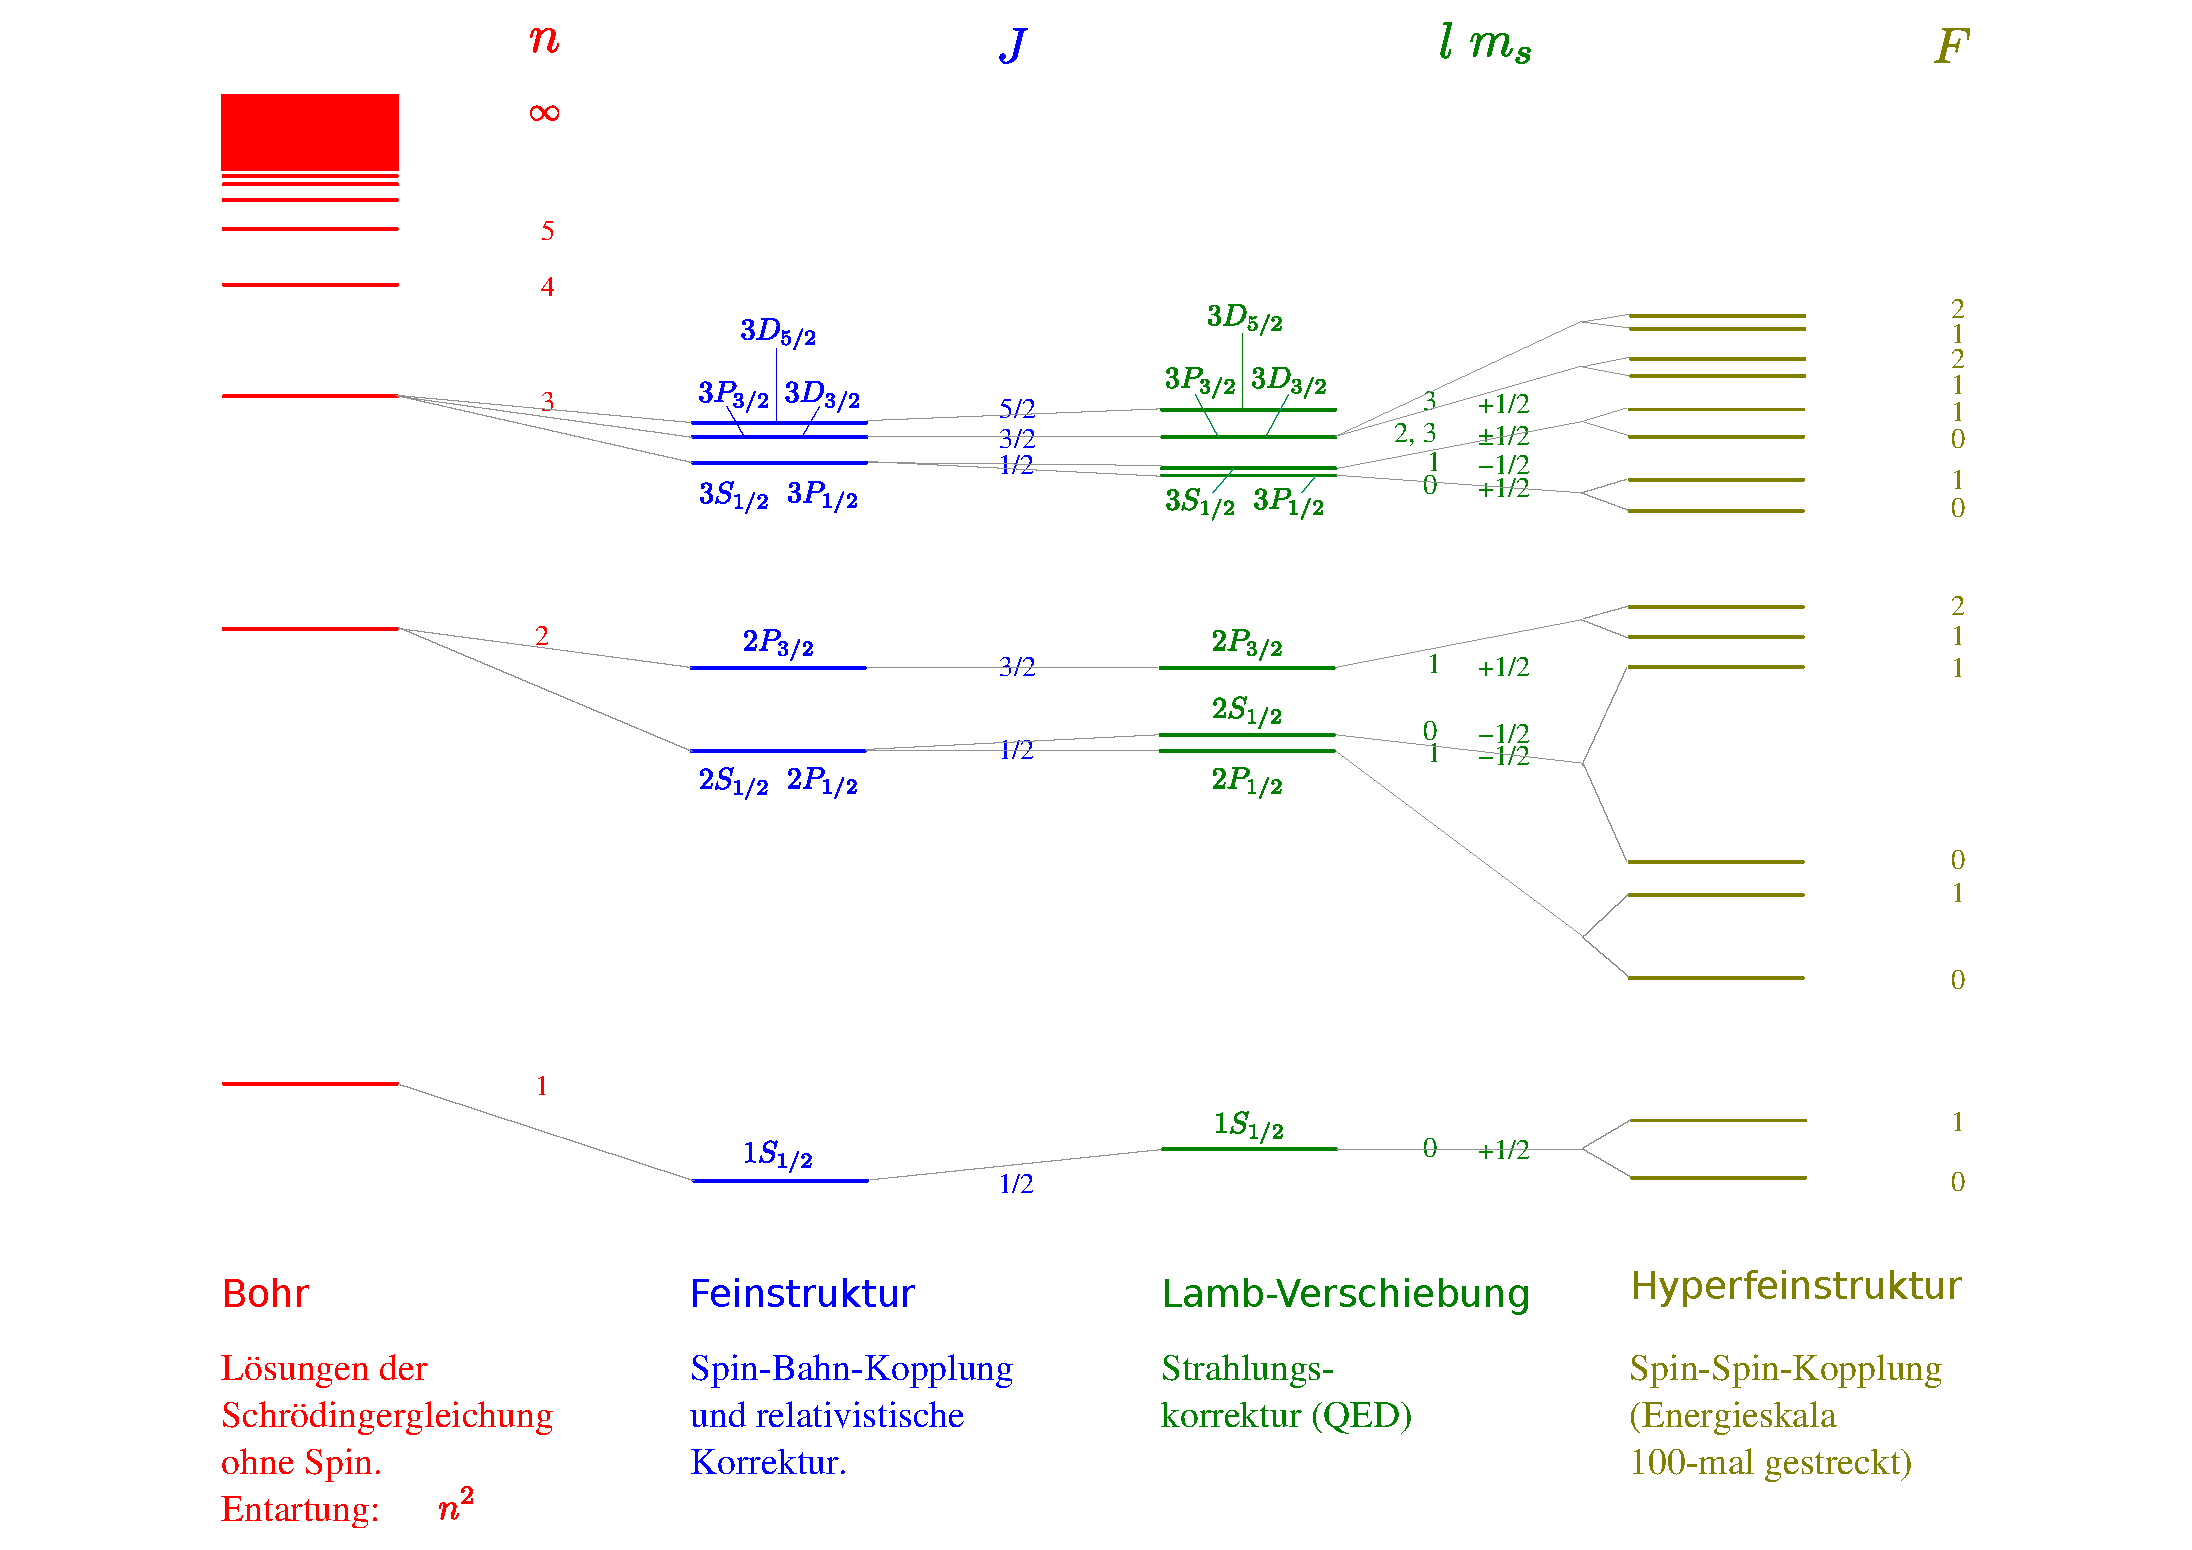
\includegraphics[width=\hsize]{images/WasserstoffAufspaltung.pdf}
\caption{Aufspaltung der Energieniveaus des Wasserstoffatoms (links)
durch die verschiedenen Effekte.
\label{skript:wasserstoffaufspaltung}}
\end{figure}
Die St"orungstheorie kann so die tats"achlich beobachteten Spektren
mindestens qualitativ erkl"aren.
In Abbildung~\ref{skript:wasserstoffaufspaltung} sind links die Energieniveaus
des Wasserstoffatoms dargestellt, wie wir sie im Kapitel~\ref{chapter:wasserstoff}
berechnet haben.
Alle Niveaus sind hochgradig entartet.
Wir werden sp"ater sehen, dass sich die entarteten Zust"ande des
Wasserstoffatoms mit Hilfe des Drehimpuls unterscheiden lassen.
Der Drehimpuls "aussert sich in magnetischen Eigenschaften,
"aussere Magnetfelder oder das vom Spin herr"uhrende magnetische Dipolmoment
der Elektronen spaltet daher die Energieniveaus auf.
Der Grundzustand hat keinen Drehimpuls, er wird daher nur wenig
aufgespalten.

%
% XXX Zeitabhaengige Stoerungstheorie
%
%\section{Zeitabh"angige St"orungstheorie}

\section*{"Ubungsaufgaben}
\rhead{"Ubungsaufgaben}
\begin{uebungsaufgaben}
\item
Die Keplergleichung wird in der Himmelsmechanik gebraucht, um die 
Position von Planeten und Satellition in Abh"angigkeit von der Zeit
zu berechnen, die sich auf elliptischen Bahnen bewegen.
Zu gegebenem $M$ ist die Zahl $E$ zu finden, f"ur die die Gleichung
\[
E-e\sin E=M
\]
gilt.
Die Zahl $e$ ist die Exzentrizit"at der Ellipsenbahn. F"ur $e=0$
geht die Ellipse in einen Kreis "uber, und die Gleichung ist trivial
zu l"osen. Finden sie eine St"orungsl"osung vierter Ordnung
der Kepler-Gleichung in Abh"angigkeit von $e$ als St"orungsparameter.

\begin{loesung}
Wir setzen $E$ als Funktion von $e$ an
\[
E(e)
=
E_0+E_1e+E_2e^2+\dots
\]
Dies setzen wir in die Keplergleichung ein
\begin{align*}
M
&=
E(e)-e\sin E(e)
\\
&=
E_0+E_1e+E_2e^2+\dots
-e\biggl(
E(e)-\frac1{3!}E(e)^3+\dots
\biggr)
\\
&=
E_0+E_1e+E_2e^2+E_3e^3+E_4e^4+\dots
-e\biggl(
E_0+E_1e+E_2e^2+E_3e^3+E_4e^4+\dots
-E_0^3e^3-\dots
\biggr)
\end{align*}
weitere Terme auf der rechten Seite m"ussen nicht ber"ucksichtigt
werden, weil sie h"ohere Ordnung als 4 haben.
Es bleibt also die Gleichung
\begin{align*}
M
&=
E_0+E_1e+E_2e^2+E_3e^3+E_4e^4
-E_0e-E_1e^2-E_2e^3-E_3e^4
+E_0^3e^4+\dots
\\
&=
E_0
+(E_1-E_0)e
+(E_2-E_1)e^2
+(E_3-E_2)e^3
+(E_4-E_3+E_0^3)e^4
\end{align*}
Aus dem Koeffizientenvergleich k"onnen wir jetzt die Koeffizienten ablesen
\begin{equation}
\begin{aligned}
E_0&=M
\\
E_1-E_0&=0&&\Rightarrow&E_1&=E_0=M\\
E_2-E_1&=0&&\Rightarrow&E_2&=E_1=M\\
E_3-E_2&=0&&\Rightarrow&E_3&=E_2=M\\
E_4-E_3+E_0^3&=0&&\Rightarrow&E_4&=E_3-E_0^3=M-M^3
\end{aligned}
\end{equation}
Die St"orungsreihe bis zur vierten Ordnung f"ur $E$ ist also
\[
E(e)=M+Me+Me^2+Me^3+(M-M^3)e^4.
\]
\end{loesung}


\item
Gegeben ist die Matrix
\[
H(\varepsilon)
=
\begin{pmatrix}\varepsilon&1\\1&-\varepsilon\end{pmatrix}
=
\begin{pmatrix}0&1\\1&0\end{pmatrix}
+
\varepsilon
\begin{pmatrix}1&0\\0&-1\end{pmatrix}
.
\]
Finden Sie eine St"orungsl"osung erster Ordnung f"ur Eigenwerte und
Eigenvektoren von $H(\varepsilon)$ in Abh"angigkeit vom St"orungsparameter
$\varepsilon$.

\begin{loesung}
Zun"achst brauchen wir die exakte L"osung f"ur den ungest"orten Fall,
also f"ur $\varepsilon=0$. Das charakteristische Polynom ist
\[
\left|
\begin{matrix}-\lambda&1\\1&-\lambda\end{matrix}
\right|
=\lambda^2-1=(\lambda+1)(\lambda-1)=0,
\]
die Eigenwerte sind also $\lambda_\pm=\pm 1$. Die zugeh"origen
Eigenvektoren k"onnen mit dem Gaussalgorithmus berechnet werden:
\[
\begin{aligned}
\begin{tabular}{|>{$}c<{$}>{$}c<{$}|}
\hline
-1&1\\
1&-1\\
\hline
\end{tabular}
&\rightarrow
\begin{tabular}{|>{$}c<{$}>{$}c<{$}|}
\hline
1&-1\\
0&0\\
\hline
\end{tabular}
&&\Rightarrow&
v_+&=\frac1{\sqrt{2}}\begin{pmatrix}1\\1\end{pmatrix}
\\
\begin{tabular}{|>{$}c<{$}>{$}c<{$}|}
\hline
1&1\\
1&1\\
\hline
\end{tabular}
&\rightarrow
\begin{tabular}{|>{$}c<{$}>{$}c<{$}|}
\hline
1&1\\
0&0\\
\hline
\end{tabular}
&&\Rightarrow&
v_+&=\frac1{\sqrt{2}}\begin{pmatrix}1\\-1\end{pmatrix}
\end{aligned}
\]
Auf diese ungest"orte L"osung k"onnen wir jetzt die St"orungstheorie
anwenden.

Nach der allgemeinen Theorie k"onnen wir die Korrekturterme f"ur die
Eigenwerte und Eigenvektoren mit den Formeln (\ref{stoerungsloesung1ordnung})
berechnen.
\begin{align*}
E_+^{(1)}&=v_+^tH_1v_+
	=\frac12\begin{pmatrix}1&1\end{pmatrix}
		\begin{pmatrix}1&0\\0&-1\end{pmatrix}
		\begin{pmatrix}1\\1\end{pmatrix}
	=\frac12\begin{pmatrix}1&1\end{pmatrix}
		\begin{pmatrix}1\\-1\end{pmatrix}
	=0
\\
E_-^{(1)}&=v_-^tH_1v_-=0
	=\frac12\begin{pmatrix}1&-1\end{pmatrix}
		\begin{pmatrix}1&0\\0&-1\end{pmatrix}
		\begin{pmatrix}1\\-1\end{pmatrix}
	=\frac12\begin{pmatrix}1&-1\end{pmatrix}
		\begin{pmatrix}1\\1\end{pmatrix}
	=0
\end{align*}
In erster Ordnung werden die Eigenwerte also nicht ver"andert.
Die gemischten Koeffizienten sind
\begin{align*}
\frac{v_+^tH_1v_-}{E_+-E_-}
&=
\frac{1}{2}
\frac12
	\begin{pmatrix}1&-1\end{pmatrix}
	\begin{pmatrix}1&0\\0&-1\end{pmatrix}
	\begin{pmatrix}1\\1\end{pmatrix}
=
-\frac14
	\begin{pmatrix}1&-1\end{pmatrix}
	\begin{pmatrix}1\\-1\end{pmatrix}
=
-\frac12
\\
\frac{v_-^tH_1v_+}{E_--E_+}
&=
\frac{1}{-2}
\frac12
	\begin{pmatrix}1&1\end{pmatrix}
	\begin{pmatrix}1&0\\0&-1\end{pmatrix}
	\begin{pmatrix}1\\-1\end{pmatrix}
=
\frac14
	\begin{pmatrix}1&1\end{pmatrix}
	\begin{pmatrix}-1\\-1\end{pmatrix}
=
-\frac12
\end{align*}
Damit sind die neuen Eigenvektoren:
\begin{align*}
v_+(\varepsilon)
&=
(1+i\varepsilon\gamma)
\frac1{\sqrt{2}}
\begin{pmatrix}1\\-1\end{pmatrix}
-\varepsilon\frac1{2\sqrt{2}}\begin{pmatrix}1\\1\end{pmatrix}
\\
v_-(\varepsilon)
&=
(1+i\varepsilon\gamma)
\frac1{\sqrt{2}}
\begin{pmatrix}1\\1\end{pmatrix}
-\varepsilon\frac1{2\sqrt{2}}\begin{pmatrix}1\\-1\end{pmatrix}
\end{align*}
Darin ist $\gamma$ so zu w"ahlen, dass die Vektoren L"ange $1$ erhalten.
\end{loesung}


\end{uebungsaufgaben}

\chapter{Magnetfeld}
\lhead{Magnetfeld}
\rhead{}
\index{Lorentz-Kraft}
\index{Magnetfeld}
Elektronen interagieren auch mit Magnetfeldern. Die Lorentz-Kraft
steht aber immer senkrecht auf der Bahn eines Teilchens, insbesondere
leistet sie keine Arbeit, und kann daher auch nicht in die Energie
eingehen.
Es braucht daher eine grundlegend andere Beschreibung des Magnetfeldes
und der Hamilton-Funktion, um Magentfelder in den Formalismus
integrieren zu k"onnen.

\section{Vektorpotential}
F"ur die quantenmechanische Beschreibung eines Teilchens in einem
elektrischen Feld konnten wir das Potential verwenden, welches
direkt die Energie eines Teilchens aus der Position zu bestimmen
erlaubt. 
Das elektrische Feld $\vec E$ kann aus dem Potential mittels
\[
\vec E=\operatorname{grad}\varphi
=
\begin{pmatrix}
\frac{\partial\varphi}{\partial x}\\
\frac{\partial\varphi}{\partial y}\\
\frac{\partial\varphi}{\partial z}
\end{pmatrix}
\]
rekonstruiert werden.
Das Magnetfeld hat kein Potential, aus dem es als Gradient wiedergewonnen
werden k"onnte, und die Kr"afte, die das Magnetfeld
auf ein Teilchen aus"ubt sind nicht vom Ort, sondern von der Geschwindigkeit
abh"angig.

Zum Magnetfeld gibt es trotzdem eine "ahnliche Konstruktion.
Das Magnetfeld $\vec B$ hat keine Quellen, es gibt keine magnetischen
Monopole.
Mathematisch kann man dies dadurch ausdr"ucken, dass 
\[
\operatorname{div}\vec B
=
\frac{\partial B_x}{\partial x}
+
\frac{\partial B_y}{\partial y}
+
\frac{\partial B_z}{\partial z}
=0
\]
ist.
Man kann zeigen, dass es zu so einem Vektorfeld ein Vektorfeld $\vec A$
gibt, aus dem sich das Magnetfeld mit der Formel
\[
\vec B=\operatorname{rot}\vec A
=\begin{pmatrix}
\frac{\partial A_3}{\partial y}-\frac{\partial A_2}{\partial z}\\
\frac{\partial A_1}{\partial z}-\frac{\partial A_3}{\partial x}\\
\frac{\partial A_2}{\partial x}-\frac{\partial A_1}{\partial y}
\end{pmatrix}
\]
rekonstruieren l"asst.

\begin{beispiel}
Sei $\vec B_0$ ein fester Vektor, und betrachten das Feld
\[
\vec A=\frac12\vec B_0\times \vec r=\begin{pmatrix}
B_2z-B_3y\\
B_3x-B_1z\\
B_1y-B_2x
\end{pmatrix}
\]
Das zugeh"orige Magnetfeld ist
\begin{equation}
\vec B
=
\operatorname{rot}\vec A
=
\frac12
\begin{pmatrix}
\frac{\partial}{\partial y}(B_1y-B_2x)-\frac{\partial}{\partial z}(B_3x-B_1z)\\
\frac{\partial}{\partial z}(B_2z-B_3y)-\frac{\partial}{\partial x}(B_1y-B_2x)\\
\frac{\partial}{\partial x}(B_3x-B_1z)-\frac{\partial}{\partial y}(B_2z-B_3y)
\end{pmatrix}
=
\begin{pmatrix}
B_1\\B_2\\B_3
\end{pmatrix}
\end{equation}
Dieses Vektorfeld $\vec A$ geh"ort zum homogenen Magnetfeld $\vec B_0$.
\end{beispiel}

\section{Hamilton-Funktion f"ur ein Teilchen im Magnetfeld}
Wie sieht die Hamilton-Funktion eines Teilchens aus, welches  sich in
einem Magnetfeld $\vec B$ bewegt?
Das Feld $\vec B$ kann in der Hamilton-Funktion nicht direkt
verwendet werden, denn da die Lorentz-Kraft immer senkrecht
auf dem Feld $\vec B$ steht, leistet $\vec B$ keine Arbeit, und kann
daher auch keinen Beitrag zu Energie leisten.

Mit dem Laplace-Formalismus kann man die korrekte Form der
Hamilton-Funktion finden.
Dabei zeigt sich, dass man eine andere Impulskoordinate $\vec P$
an Stelle der bekannten Impulse $\vec p$ verwenden muss. 
Die neue Impulskoordinate ist 
\[
\vec P = \vec p + e\vec A,
\]
sie beinhaltet das Vektorpotential.
Dadurch werden die Impulse und das Vektorpotential miteinander 
verkn"upft, wir m"ussen nur kontrollieren, ab die Verkn"upfung
tats"achlich so ist, dass die Bewegungsgleichungen uns auf die
Lorentz-Kraft f"uhren.

Die kinetische Energie muss n"aturlich mit den Impulsen $\vec p$ ausgedr"ucket
werden, die mittels $\vec p=\vec P-e\vec A$ durch $\vec P$
ausgedr"uckt werden k"onnen.
Die Hamilton-Funktion f"ur ein Teilchen in einem Potential $\varphi$
und Vektorpotential $\vec A$ wird damit zu
\begin{equation}
H(\vec P, \vec x)=\frac1{2m}(\vec P-e\vec A)^2+e\varphi.
\label{hamiltonmitmagnetfeld}
\end{equation}

Wir verifizieren, dass die Bewegungsgleichungen, die sich aus dieser
Hamilton-Funktion ergeben, tats"achlich die Lorentzkraft auf ein
Teilchen im Magnetfeld richtig wiedergeben.
Zun"achst rechnen wir die Bewegungsgleichungen aus
\begin{align*}
\frac{dx_i}{dt}
&=
\frac{\partial H}{\partial P_i}
=
\frac1m(P_i-eA_i)
\\
\frac{dP_i}{dt}
&=
-\frac{\partial H}{\partial x_i}
=
\frac{e}{m}\sum_{j=1}^3( P_j-eA_j)\frac{\partial A_j}{\partial x_i}
-e\frac{\partial\varphi}{\partial x_i}
=
e\sum_{j=1}^3\frac{p_j}{m}\frac{\partial A_j}{\partial x_i}
-e\frac{\partial\varphi}{\partial x_i}
=
e\sum_{j=1}^3v_j\frac{\partial A_j}{\partial x_i}
-e\frac{\partial\varphi}{\partial x_i}
\end{align*}
Wir m"ussen die Bewegungsgleichungen in der Newtonschen Form 
finden, denn nur so k"onnen wir die Kr"afte identifizieren.
Wir leiten daher die erste Gleichung nochmals nach der Zeit ab,
und erhalten
\[
\frac{d^2 x_i}{dt^2}
=
\frac1m\frac{dP_i}{dt}-\frac{e}{m}\biggl(
\frac{\partial A_i}{\partial t}
+\sum_{j=1}^3\frac{\partial A_i}{\partial x_j}\frac{dx_j}{dt}
\biggr)
=
\frac1m\frac{dP_i}{dt}-\frac{e}{m}\biggl(
\frac{\partial A_i}{\partial t}
+
\sum_{j=1}^3\frac{\partial A_i}{\partial x_j}v_j
\biggr)
\]
Darin k"onnen wir die Ableitung von $P_i$ nach der Zeit aus der
zweiten Hamiltonschen Bewegungsgleichung einsetzen:
\begin{align*}
m\frac{d^2 x_i}{dt^2}
&=
e\sum_{j=1}^3v_j\frac{\partial A_j}{\partial x_i}
-e\frac{\partial\varphi}{\partial x_i}
-
e\biggl(
\frac{\partial A_i}{\partial t}
+\sum_{j=1}^3\frac{\partial A_i}{\partial x_j}v_j
\biggr)
\end{align*}
Dies wird "ubersichtlicher, wenn wir die rechte Seite f"ur $i=1$
ausrechnen:
\begin{align*}
m\frac{d^2 x_i}{dt^2}
&=
e\biggl(
v_1\frac{\partial A_1}{\partial x_1}
+
v_2\frac{\partial A_2}{\partial x_1}
+
v_3\frac{\partial A_3}{\partial x_1}
-
v_1\frac{\partial A_1}{\partial x_1}
-
v_2\frac{\partial A_1}{\partial x_2}
-
v_3\frac{\partial A_1}{\partial x_3}
\biggr)
-e\frac{\partial\varphi}{\partial x_i}
-e\frac{\partial A_i}{\partial t}
\\
&=
e\biggl(
v_2\frac{\partial A_2}{\partial x_1}
+
v_3\frac{\partial A_3}{\partial x_1}
-
v_2\frac{\partial A_1}{\partial x_2}
-
v_3\frac{\partial A_1}{\partial x_3}
\biggr)
-e\frac{\partial\varphi}{\partial x_i}
-e\frac{\partial A_i}{\partial t}
\\
&=
e\biggl(
v_2
\biggl(
\frac{\partial A_2}{\partial x_1}
-
\frac{\partial A_1}{\partial x_2}
\biggr)
-
v_3\biggr(
\frac{\partial A_1}{\partial x_3}
-
\frac{\partial A_3}{\partial x_1}
\biggr)
\biggr)
-e\frac{\partial\varphi}{\partial x_i}
-e\frac{\partial A_i}{\partial t}
\\
&=
e\biggl(
v_2B_3
-
v_3B_2
\biggr)
-e\frac{\partial\varphi}{\partial x_i}
-e\frac{\partial A_i}{\partial t}
\end{align*}
In dieser Form stehen die Kr"afte auf der rechten Seite. 
In vektorieller Form
\[
m\frac{d^2\vec x}{dt^2}
=
e\vec v\times\vec B
-e\operatorname{grad}\varphi
-e\frac{\partial\vec A}{\partial t}
\]
erkennt man die Kr"afte: der erste Term ist die Lorentz-Kraft,
der zweite ist das elektrische Feld mit Potential $\varphi$.

\section{Hamilton-Operator im Magnetfeld}
Die Bewegung eines quantenmechanischen Teilchens erhalten wir jetzt
aus dem Hamilton-Operator mit den "ublichen Quantisierungsregeln.
Die Impulse $P_i$ m"ussen durch Ableitungsoperatoren ersetzt werden.
Der Hamiltonoperator in Ortsdarstellung ist also
\[
H=\frac1{2m}\sum_{k=1}^3\biggl(
\frac{\hbar}{i}
\frac{\partial}{\partial x_k}
-eA_k
\biggr)^2
+e\varphi.
\]
Man kann ihn zum Beispiel verwenden, um den Einfluss eines Magnetfeldes
auf die Elektronen in einem Atom zu messen.
Zum Beispiel kann man ein homogenes Magnetfeld in $z$-Richtung
aus dem Vektorpotential
\[
\vec A=\begin{pmatrix}
-yB\\0\\0
\end{pmatrix}
\qquad
\Rightarrow
\qquad
\vec B=\operatorname{rot}\vec A
=\begin{pmatrix}
\frac{\partial A_3}{\partial y}-\frac{\partial A_2}{\partial z}\\
\frac{\partial A_1}{\partial z}-\frac{\partial A_3}{\partial x}\\
\frac{\partial A_2}{\partial x}-\frac{\partial A_1}{\partial y}
\end{pmatrix}
=
\begin{pmatrix}
0\\0\\B
\end{pmatrix}
\]
bekommen.
Ein Teilchen in einem homogenen Magnetfeld hat daher den Hamilton-Operator
\[
H
=
\frac1{2m}\biggl(\frac{\hbar}{i}\frac{\partial}{\partial x}+eBy\biggr)^2
-\frac{\hbar^2}{2m}\frac{\partial^2}{\partial y^2}
-\frac{\hbar^2}{2m}\frac{\partial^2}{\partial z^2}
\]
Man beachte, dass jetzt der Impulsoperator in $y$-Richtung nicht mehr
mit dem Impulsoperator in $x$-Richtung vertauscht, man kann also
nicht gleichzeitig die $x$- und $y$-Impuls wissen.
Allerdings vertauscht den die Impulsoperatoren in $x$- und $z$-Richtung
immer noch mit $H$, diese Impulskomponenten sind also Erh"altungsgr"ossen.

Man kann versuchen, eine L"osung der Schr"odingergleichung f"ur $H$ mit
einem Ansatz
\[
\psi(x,y,z)
=
e^{\frac{i}{\hbar}(xp_x+zp_z)}Y(y)
\]
zu finden.
Setzt man diesen Ansatz in die Schr"odingergleichung ein, bekommt man
\begin{align}
e^{\frac{i}{\hbar}(xp_x+zp_z)}
\biggl(
\frac1{2m}
(p_x+eyB)^2
Y(y)
-
\frac1{2m}
\hbar^2 Y''(y)
+
\frac1{2m}p_z^2
Y(y)
\biggr)
&=
E
e^{\frac{i}{\hbar}(xp_x+zp_z)}
Y(y)
\notag
\\
-\frac{\hbar^2}{2m} Y''(y)
+
\biggl(
-E
+
\frac{ p_z^2}{2m}
+
\frac1{2m}
(p_x+eyB)^2
\biggr)
Y(y)
&=
0
\label{Ygl}
\end{align}
Indem wir schreiben
\[
y_0=-\frac{p_x}{eB}
\qquad
\text{und}
\qquad
\omega_B
=\frac{eB}{m}
\]
erhalten wir aus (\ref{Ygl}) die Differentialgleichung
\begin{equation}
-\frac{\hbar}{2m}Y''
+\frac{m}2\omega_B^2(y-y_0)^2Y
=
\biggl(E-\frac{p_z^2}{2m}\biggr) Y
\label{landauniveaus}
\end{equation}
Dies ist die Eigenwertgleichung eines harmonischen Oszillators mit
Kreisfrequenz $\omega_B$.
Dessen Energieniveaus haben wir im Kapitel~\ref{chapter:harmonischeroszillator}
bereits berechnet, sie sind Vielfachen von $\hbar\omega_B$, insbesondere
gilt:
\[
\biggl(E-\frac{p_z^2}{2m}\biggr) = \hbar\omega_B\biggl(n+\frac12\biggr)
\qquad\Rightarrow\qquad
E=
\hbar\omega_B\biggl(n+\frac12\biggr)
-
\frac{p_z^2}{2m}
\]
Bei gegebenem Impuls in $x$- und $z$-Richtung ist die Bewegung in
$y$-Richtung als quantisiert.
Die zul"assigen Energieniveaus unterscheiden sich 

Man kann sich dieses Ph"anomen auch klassisch vorstellen.
Die Lorentzkraft zwingt Elektronen in Spiralbahnen um die Feldlinien des
Magnetfeldes.
Betrachtet man die Teilchen als Wellen, muss eine Umlauf um die
Feldlinie zu konstruktiver Interferenz f"uhren, daher sind nur
ganz bestimmte Phasenfrequenzen erlaubt.

\section{Eichtransformationen}
Das Vektorpotential ist die physikalisch entscheidende Gr"osse.
Im Bohm-Aharonov-Experiment
werden Elektronen durch ein Gebiet geleitet, in dem sich $\vec A$,
aber nicht $\vec B$ "andert, trotzdem stellt das Experiment eine
Beeinflussung fest.

Das Vektorpotential ist nicht eindeutig: wenn man zu $\vec A$
den Gradienten einer Funktion $\chi$ hinzuaddiert, "andert sich
$\vec B$ nicht, weil
\[
\operatorname{rot}(\vec A+\operatorname{grad}\chi)
=
\underbrace{\operatorname{rot}\vec A}_{\vec B}
+
\underbrace{\operatorname{rot}\operatorname{grad}\chi}_{=0}
=
\vec B.
\]

Wenn das Vektorpotential die physikalisch ``reale'' Gr"osse ist,
sie aber nicht eindeutig ist, dann d"urfen sich keine messbaren
Gr"ossen "andern, wenn man $\vec A$ auf zul"assige Art "andert.
In der Quantenmechanik bedeutet das, dass sich die Wahrscheinlichkeiten
nicht "andern d"urfen, d.~h.~die Wellenfunktion darf sich h"ochstens
um einen Phasenfaktor "andern.

Wir gehen daher davon aus, dass $\psi$ eine Wellenfunktion ist,
die die Schr"odingergleichung des Hamilton-Operators mit Vektorpotential
$\vec A$ l"ost,
dass also
\[
\frac{\hbar}{i}\frac{\partial}{\partial t}\psi
=
H\psi
\]
Wenn wir die Ersetzung
$\vec A\mapsto \vec A+\operatorname{grad}\chi$
im Hamilton-Operator durchf"uhren, m"ussen wir die Wellenfunktion
mit einem Phasenfaktor $e^{if(x)}$ korrigieren.
Die Wirkung des modifizierten Impulsoperators ist
\begin{align*}
\biggl(
\frac{\hbar}{i}\frac{\partial}{\partial x_k}+eA_k
+\frac{\partial\chi}{\partial x_k}
\biggr)e^{if(x)}\psi(x)
&=
e^{if(x)}
\biggl(
\frac{\hbar}{i}\frac{\partial}{\partial x_k}+eA_k
+\frac{\partial\chi}{\partial x_k}
\biggr)
\psi(x)
+
e^{if(x)}
\frac{\hbar}{i}i\frac{\partial f}{\partial x_k}\psi(x)
\end{align*}
Die Addition von $\operatorname{grad}\chi$ zum Vektorpotential
kann nur dann ohne Folgen f"ur die Physik sein, wenn der
zus"atzlich auf der rechten Seite auftauchende Term den
Term mit $\chi$ kompensiert, wenn also gilt
\[
\frac{\partial\chi}{\partial x_k}=\hbar\frac{\partial f}{\partial x_k},
\]
oder $\operatorname{grad}\chi=\frac1{\hbar}\operatorname{grad}\chi$.
Wenn man also das Vektorpotential um $\operatorname{grad}\chi$ "andert,
muss man die Wellenfunktion um $e^{\frac{i}{\hbar}\chi}$. 
Setzt man dies jedoch auf der linken Seite der zeitabh"angigen
Schr"odingergleichung ein, erh"alt man
\[
\frac{\hbar}{i}\frac{\partial}{\partial t}
\bigl(
e^{\frac{i}{\hbar}\chi}
\psi
\bigr)
=
e^{\frac{i}{\hbar}\chi}
\frac{\partial\chi}{\partial t}
\psi
+
e^{\frac{i}{\hbar}\chi}
\frac{\partial}{\partial t}
\psi
\]
Wenn sich also die Schr"odingergleichung nicht "andern soll, dann
muss der Summand $\partial\chi/\partial t$ zum Potential im
Hamilton-Operator geschlagen werden.
Wenn man also alle "Anderungen
\begin{align}
\vec A&\mapsto \vec A + \operatorname{grad}\chi
&
\varphi&\mapsto \varphi-\frac{\partial\chi}{\partial t}
&
\psi
&\mapsto
e^{\frac{i}{\hbar}\chi}\psi
\label{eichtransformation}
\end{align}
gleichzeitig durchf"uhrt, dann "andert sich physikalisch nichts,
auch wenn sich sowohl das Vektorpotential als auch das
elektrische Potential "andert.

Die Transformation (\ref{eichtransformation}) heisst Eichtransformation.
Die Schr"odingergleichungen sind invariant bez"uglich Eichtransformationen.



\chapter{Drehimpuls\label{chapter:drehimpuls}}
\lhead{Drehimpuls}
\rhead{}
Der Drehimpuls ist eine wichtige Erhaltungsgr"osse in der klassischen
Mechanik. Wir sollten in der Lage sein, einen entsprechenden Operator
f"ur den quantenmechanischen Drehimpuls zu konstruieren.

\section{Drehimpulsoperatoren\label{section:drehimpulsoperatoren}}
\rhead{Drehimpulsoperatoren}
In der klassischen Mechanik ist der Drehimpulsvektor definiert
als $\vec L=\vec r\times \vec p$. Die einzelnen Komponenten k"onnen
ausgerechnet werden:
\begin{align*}
L_1&=X_2P_3-X_3P_2,\\
L_2&=X_3P_1-X_1P_3,\\
L_3&=X_1P_2-X_2P_1.
\end{align*}
\index{Drehimpuls!Komponenten}
Auf die Reihenfolge der $x$- und $p$-Komponenten kommt es nicht an,
weil nur Produkte von Orts- und Impuls-Operatoren f"ur verschiedene
Richtungen verwendet werden.

Ausser dem Vektor $\vec L$ ist auch seine L"ange erhalten, also
die Gr"osse
\[
\vec L^2=L_1^2+L_2^2+L_3^2.
\]
\index{Drehimpuls!Betrag}
Wir erwarten, dass auch in der Quantenmechanik der Drehimpuls
erhalten ist, dass also sowohl die einzelnen Komponenten $L_i$ 
als auch der Betrag $\vec L^2$ mit dem Hamilton-Operator vertauschen.

Wir werden daher zun"achst die algebraischen Eigenschaften, insbesondere
die Vertauschungsrelationen bestimmen. Damit k"onnen wir dann "ahnlich
wie beim harmonischen Oszillator die Drehimpulszust"ande ermitteln.
Die Drehimpulsoperatoren in Ortsdarstellung werden wir als Teile
des Laplace-Operators wiedererkennen, den wir bei der Berechnung
des Wasserstoffatoms bereits analysiert haben. Dies wird uns erlauben,
die Quantenzahlen $l$ und $m$ der Wasserstoffzust"ande als
Drehimpuls-Quantenzahlen zu verstehen.

\section{Algebraische Eigenschaften\label{section:drehimpulsalgebra}}
\rhead{Drehimpulsalgebra}
Zun"achst erinnern wir an die grundlegenden Vertauschungsrelationen zwischen
Ort und Impuls:
\[
[P,X]=i\hbar \operatorname{id}
\]
oder die "aquivalente Formulierung
\[
PX=XP+i\hbar \operatorname{id}.
\]
Daraus sollen jetzt schrittweise die Vertauschungsrelationen f"ur die
Drehimpulskomponenten und f"ur $\vec L^2$ abgeleitet werden.
Die zweite Form der Relation erlaubt, $P$-Faktoren immer nach rechts zu
bringen, und so f"ur jeden Ausdruck in $X_i$ und $P_i$ eine
``Standardform'' zu finden, so dass solche ausdr"ucken sogar algorithmisch
miteinander verglichen werden k"onnen.

Zun"achst berechnen wir die Vertauschungsrelationen der
Drehimpulskomponenten mit $X$ und $P$:
\index{Drehimpuls!Vertauschungsrelationen}
\begin{align*}
[X_1,L_1]&=0\\
[X_2,L_1]
&=
X_2X_2P_3-X_2X_3P_2-X_2P_3X_2+X_3P_2X_2
=X_3[P_2,X_2]
=i\hbar X_3
\\
[X_3,L_1]
&=
X_3X_2P_3-X_3X_3P_2-X_2P_3X_3+X_3P_2X_3
%= X_3X_2P_3 - X_2P_3X_3
=
-X_2[P_3,X_3]
=
-i\hbar X_2
\\
[P_1,L_1]&=0\\
[P_2,L_1]
&=
P_2X_2P_3 - P_2X_3P_2 - X_2P_3P_2 + X_3P_2P_2
=
P_3[P_2,X_2]
=
i\hbar P_3
\\
[P_3,L_1]
&=
P_3X_2P_3 - P_3X_3P_2 - X_2P_3P_3 + X_3P_2P_3
=
-P_2[P_3,X_3]=-i\hbar P_2
\end{align*}
Weitere Vertauschungsrelationen k"onnen durch zyklische Vertauschung
gewonnen werden:
\begin{align*}
[X_1,L_1] &= 0          & [X_1,L_2] &=-i\hbar X_3 & [X_1,L_3] &= i\hbar X_2\\
[X_2,L_1] &= i\hbar X_3 & [X_2,L_2] &= 0          & [X_2,L_3] &=-i\hbar X_1\\
[X_3,L_1] &=-i\hbar X_2 & [X_3,L_2] &= i\hbar X_1 & [X_3,L_3] &= 0         \\
[P_1,L_1] &= 0          & [P_1,L_2] &=-i\hbar P_3 & [P_1,L_3] &= i\hbar P_2\\
[P_2,L_1] &= i\hbar P_3 & [P_2,L_2] &= 0          & [P_2,L_3] &=-i\hbar P_1\\
[P_3,L_1] &=-i\hbar P_2 & [P_3,L_2] &= i\hbar P_1 & [P_3,L_3] &= 0
\end{align*}
Die Drehimpulskomponenten vertauschen mit den Orts- und Impulskomponenten
mit gleicher Richtung, aber nicht mit den anderen.
Man kann von einem Teilchen also gleichzeitig nur die Impulskomponente
und die dazu parallele Drehimpulskomponente wissen. 
Oder: vollst"andige Kenntnis des Drehimpulses schliesst vollst"andige
Kenntnis des Bewegungszustandes aus.

Es fragt sich allerdings auch, ob man "uberhaupt vollst"andige Kenntnis
des Drehimpulszustandes haben kann.
Dazu m"ussen die Kommutatoren der Drehimpulskomponenten untereinander
berechnet werden:
\begin{align}
[L_1,L_2]
&=
[X_2P_3-X_3P_2,L_2]
=
X_2[P_3,L_2]-P_2[X_3,L_2]
=
X_2i\hbar P_1-P_2i\hbar X_1
=
i\hbar L_3.
\label{drehimpulskommutator}
\\
[L_2,L_3]&=i\hbar L_1
\notag
\\
[L_3,L_1]&=i\hbar L_2
\notag
\\
\{L_1,L_2\}
&=
L_1L_2+L_2L_1=i\hbar L_3+2L_2L_1
\label{drehimpulsantikommutator}
\end{align}
Die zweite und dritte Relation haben wir durch zyklische Vertauschung
gewonnen.
Die Drehimpulskomponenten vertauschen untereinander nicht, es ist also
nicht m"oglich, zwei Drehimpulskomponenten eines Teilchens
gleichzeitig exakt zu wissen.
Es gibt keine Zust"ande, die Eigenzust"ande f"ur mehr als einen
der Operatoren f"ur die Drehimpulskomponenten ist.

Die gleiche Frage k"onnen wir auch stellen f"ur den Gesamtdrehimpuls
$\vec L^2=L_1^2+L_2^2+L_3^2$. Dazu m"ussen wir Vertauschungsrelationen
verschiedener Operatoren mit den einzelnen Summanden in $\vec L^2$, also
mit $L_i^2$ berechnen.
Solche Berechnungen k"onnen vereinfacht werden durch eine Hilfsformel:

\begin{hilfssatz}
\label{commutatora2b}
Seien $A$ und $B$ Operatoren, dann gilt
\begin{align*}
[A^2,B]
&=
\{A,[A,B]\}
=
[A,\{A,B\}].
\end{align*}
\end{hilfssatz}

\begin{proof}[Beweis]
Wir schreiben den Kommutator aus:
\begin{align*}
[A^2,B]
=
AAB-BAA
&=
AAB\underbrace{\mathstrut -ABA+ABA}_{=0}\mathstrut -BAA
=
A[A,B]+[A,B]A
=
\{A,[A,B]\}
\\
&=
AAB\underbrace{\mathstrut +ABA-ABA}_{=0}\mathstrut -BAA
=
A\{A,B\}-\{A,B\}A
=
[A,\{A,B\}]
\end{align*}
\end{proof}

Wir wenden diesen Hilfssatz auf die Berechnung der Vertauschungsrelationen
der Komponenten des Drehimpulses mit $\vec L^2$ an.
Dazu werden wir die Antikommutatoren des Drehimpulses brauchen, die
wir in (\ref{drehimpulsantikommutator}) schon berechnet haben.
Wir finden:
\begin{align*}
[L_1^2,L_1]&=0
\\
[L_2^2,L_1]
&=
\{L_2,[L_2,L_1]\}
=
-\{L_2,i\hbar L_3\}
=-i\hbar\{L_2,L_3\}
\\
[L_3^2,L_1]
&=
\{L_3,[L_3,L_1]\}
=
\{L_3,i\hbar L_2\}
=
i\hbar\{L_2,L_3\}
\\
[\vec L^2, L_1]
&=
[L_1^2,L_1]
+
[L_2^2,L_1]
+
[L_3^2,L_1]
=
0
-i\hbar\{L_2,L_3\}
+
i\hbar\{L_2,L_3\}
=
0
\\
[\vec L^2,L_2]&=0
\qquad
\qquad
\text{(durch zyklische Vertauschung)}
\\
[\vec L^2,L_3]&=0
\end{align*}
Die Komponenten des Drehimpulses vertauschen untereinander zwar nicht,
aber sie vertauschen mit dem Gesamtdrehimpuls. Es ist also m"oglich,
den Gesamtdrehimpuls gleichzeitig mit einer der Komponenten zu messen,
aber es ist nicht m"oglich, mehr als eine Komponente des Drehimpulses
zu messen.

Damit stellt sich aber die Frage, ob der Gesamtdrehimpuls etwas ist,
was man unabh"angig vom Bewegungszustand messen kann.
Dazu m"ussen die Vertauschungsrelationen von $\vec L^2$ mit den
Impulskomponenten oder den Ortskomponenten bestimmt werden.
\begin{align*}
[L_1^2,X_1]
&=
\{L_1,[L_1,X_1]\}
=\{L_1,0\}=0
\\
[L_2^2,X_1]
&=
\{L_2,[L_2,X_1]\}
=
\{L_2,-i\hbar X_3\}
\\
[L_3^2,X_1]
&=
\{L_3,[L_3,X_1]\}
=
\{L_3, i\hbar X_2\}
\\
\Rightarrow\qquad
[\vec L^2,X_1]
&=
i\hbar(-L_2X_3-X_3L_2+L_3X_2+X_2L_3)
\\
&=
i\hbar(-L_2X_3-L_2X_3+i\hbar X_1 +L_3X_2+L_3X_2-i\hbar X_1)
=
2i\hbar(-L_2X_3 +L_3X_2)
\\
&=
2i\hbar(
-X_3P_1X_3+X_1P_3X_3+X_1P_2X_2-X_2P_1X_2
)
\\
&=
2i\hbar(
-(X_2^2+X_3^2)P_1+X_1X_3P_3-i\hbar X_1+ X_1X_2P_2-i\hbar X_1
)
\\
&=
2i\hbar(
-(X_2^2+X_3^2)P_1
+X_1(X_3P_3 + X_2P_2)
-2i\hbar X_1
)
\end{align*}
Eine "ahnliche Rechnung f"ur die Impulskomponenten zeigt, dass der
Drehimpulsbetrag nicht gleichzeitig mit Ort- oder Impulszustand
gemessen werden kann.
Dies ist auch physikalisch einleuchtend.
Kennt man den Ort und den Drehimpuls exakt, erh"alt man auch exakte
Information "uber den Impuls.
Da man aber Ort und Impuls nicht gleichzeitig wissen kann, muss es auch
eine Vertauschungsrelation geben, die verhindert, dass wir zu viel
gleichzeitiges Wissen "uber Ort und Drehimpuls erhalten k"onnen.

\section{Drehimpulszust"ande\label{section:drehimpulszustaende}}
\rhead{Drehimpulszust"ande}
Beim harmonischen Oszillator haben wir eine Technik kennengelernt, nicht
nur die Eigenwerte, sondern auch die Eigenvektoren algebraisch aus dem
Grundzustand des Systems abzuleiten.
Ein "ahnliches Vorgehen ist auch hier m"oglich, denn auch hier haben wir
wieder eine Observable, n"amlich $\vec L^2$, welche nur positive
Werte annehmen kann.
Unter den Eigenzust"anden dieser Observablen muss es daher solche mit
minimalem Eigenwert geben.
Wir brauchen dann nur noch Operatoren, welche uns erlauben, von einem
solchen Grundzustand des Drehimpulsoperator zu den Zust"anden 
h"oheren Drehimpulses aufzusteigen.
Wenn dieser Plan realsiert werden kann, w"urde sich auch gleich
eine weitere wichtige Aussage der Quantenmechanik ergeben: der Drehimpuls
kommt nur in Vielfachen von $\hbar$ vor.

\subsection{Eigenzust"ande von $L_3$}
\index{Drehimpuls!Eigenzust\"ande von $L_3$}
\index{Drehimpuls!Auf- und Absteigeoperatoren}
Aus den Operatoren $L_1$ und $L_2$ k"onnen wir "ahnlich wie beim
harmonischen Oszillator zwei neue Operatoren
\begin{align*}
L_+&=L_1+iL_2
&
L_-&=L_1-iL_2
\end{align*}
konstruieren.
Auch hier gilt die Einschr"ankung, dass dies keine selbstadjungierten
Operatoren sind, $L_\pm$ entspricht also nicht einer beobachtbaren
physikalischen Gr"osse. 
Immerhin ist $L_+^*=L_-$.
Diese Operatoren haben die folgenden Vertauschungsrelationen mit
den Drehimpulskomponenten:
\begin{equation}
\begin{aligned} 
\phantom{ }	% this is a workaround to prevent from the aligned environment
		% from interpreting the next commutator as an option to the
		% environment
[L_\pm, L_1]
&=
[L_1,L_1]\pm i[L_2,L_1]
=
\pm \hbar L_3
\\
[L_\pm, L_2]
&=
[L_1,L_2]\pm i[L_2,L_2]
=
i\hbar L_3
\\
[L_\pm,L_3]
&=
[L_1,L_3]\pm i[L_2,L_3]
=
-i\hbar L_2
\mp
\hbar L_1
=
\mp \hbar L_\pm
\end{aligned}
\label{lpmlkommutator}
\end{equation}
Nehmen wir jetzt an, dass $|\psi\rangle$ ein Eigenzustand von $L_3$ mit
Eigenwert $l_3$ ist, dann gilt
\[
L_3L_+\,|\psi\rangle
=
L_+L_3\,|\psi\rangle+\hbar L_+|\psi\rangle
=
l_3L_+\,|\psi\rangle+\hbar L_+|\psi\rangle
=
(l_3+\hbar)L_+\,|\psi\rangle,
\]
der Zustand $L_+\,|\rangle$ ist also wieder ein Eigenzustand von $L_3$,
allerdings ist der Eigenwert um $\hbar$ erh"oht worden.
Analog kann man aus
\[
L_3L_-\,|\psi\rangle
=
L_-L_3\,|\psi\rangle-\hbar L_-\,|\psi\rangle
=
(l_3-\hbar)L_-\,|\psi\rangle
\]
ablesen,  dass $L_-\,|\psi\rangle$ ein Eigenzustand von $L_3$ ist, dessen
Eigenwert gegen"uber dem von $|\psi\rangle$ um $\hbar$ verringert
worden ist.
Die Operatoren $L_+$ und $L_-$ haben also genau die Eigenschaften,
die wir bei den Auf- und Absteigeoperatoren beim harmonischen Oszillator
kennengelernt hatten.

Aus (\ref{lpmlkommutator}) und aus
Hilfssatz~\ref{commutatora2b} k"onnen wir jetzt die
Vertauschungsrelationen mit den Quadraten der Drehimpulskomponenten
und mit $\vec L^2$ berechnen:
\begin{align*}
\\
[L_\pm,L_1^2]
&=
\{ [L_\pm, L_1], L_1 \}
=
\{ \pm \hbar L_3, L_1 \}
=
\pm \hbar \{ L_1, L_3 \}
\\
[L_\pm,L_2^2]
&=
\{ [L_\pm, L_2], L_2 \}
=
\{ i\hbar L_3, L_2 \}
=
i\hbar \{ L_2, L_3 \}
\\
[L_\pm,L_1^2 + L_2^2]
&=
\pm \hbar \{ L_1, L_3 \}
+
i\hbar \{ L_2, L_3 \}
=
\pm \hbar \{ L_1 \mp iL_2, L_3 \}
=
\pm \hbar\{L_\pm, L_3\}
\\
[L_\pm,L_3^2]
&=
\{ [L_\pm, L_3], L_3 \}
=
\mp \{ i\hbar L_\pm, L_3 \}
=
\mp i\hbar \{ L_\pm, L_3 \}
\\
\Rightarrow\qquad [L_\pm,\vec L^2]
&=0
\end{align*}
Die Operatoren $L_\pm$ vertauschen also mit $\vec L^2$.
Ist $|\psi\rangle$ ein Eigenzustand von $\vec L^2$ mit Eigenwert $\lambda$,
dann gilt auch 
\begin{align*}
\vec L^2\,|\psi\rangle&=\lambda\,|\psi\rangle
\\
L_\pm\vec L^2\,|\psi\rangle&=
\vec L^2L_\pm\,|\psi\rangle=
\lambda L_\pm\,|\psi\rangle
\end{align*}
also ist  auch $L_\pm\,|\psi\rangle$ ein Eigenzustand von $\vec L^2$ mit
dem gleichen Eigenwert.

%Gemeinsame Eigenzust"ande $|\lambda,m\rangle$ von $\vec L^2$ und $L_3$
%mit Eigenwerten $\lambda$ und $m$ k"onnen also mit den Operatoren 
%$L_\pm$ in neue Eigenzust"ande mit gleichem $\lambda$, aber verschiedenem
%$m$ umgewandelt werden.
%\begin{align*}
%L_+|\lambda,m\rangle&=|\lambda,m+1\rangle
%L_-|\lambda,m\rangle&=|\lambda,m-1\rangle
%\end{align*}
%
\subsection{Beziehungen zwischen den Eigenwerten}
\index{Drehimpuls!Eigenwerte}
Die Drehimpulskomponenten $L_3$ ist in der klassischen Mechanik kleiner
als der Drehimpulsbetrag, und wir m"ochten nachpr"ufen, dass dies auch
in der Quantenmechanik gilt.
Dazu berechnen wir zun"achst das Produkt der Operatoren $L_+$ und $L_-$
\begin{align*}
L_+L_-
&=
L_1^2+L_2^2 +iL_2L_1-iL_1L_2=L_1^2+L_2^2 -i[L_1,L_2]=L_1^2+L_2^2+\hbar L_3
\\
L_-L_+
&=
L_1^2  + L_2^2 +i[L_1,L_2]=L_1^2+L_2^2-\hbar L_3
\\
[L_+,L_-]
&=
2\hbar L_3
\\
{\textstyle \frac12}(L_+L_-+L_-L_+)&=L_1^2+L_2^2,
\\
\vec L^2
&=
{\textstyle\frac12}(L_+L_-+L_-L_+)+L_3^2.
\end{align*}
Sei $|\lambda,l_3\rangle$ ein gemeinsamer Eigenzustand von $\vec L^2$
und $L_3$, dann muss gelten
\begin{align*}
\langle \lambda,l_3|\,\vec L^2\,|\langle, l_3\rangle
&=
\langle \lambda,l_3|
\,
{\textstyle\frac12}(L_+L_-+L_-L_+)
\,
|\lambda,l_3\rangle
+
\langle \lambda,l_3|
\,
L_3^2
\,
|\lambda,l_3\rangle
\\
\lambda
&=
\langle \lambda,l_3|
\,
{\textstyle\frac12}(L_+L_-+L_-L_+)
\,
|\lambda,l_3\rangle
+
l_3^2
\end{align*}
Der erste Term auf der rechten Seite ist aber auf jeden Fall positiv,
wie man sich durch folgende Rechnung "uberzeugen kann:
\[
\langle \lambda,l_3|
\,
{\textstyle\frac12}(L_+L_-+L_-L_+)
\,
|\lambda,l_3\rangle
=
\langle \lambda,l_3|
\,
{\textstyle\frac12}(L_-^*L_-+L_+^*L_+)
\,
|\lambda,l_3\rangle
=
\frac12\|\,L_-\,|\lambda,l_3\rangle\|^2
+
\frac12\|\,L_+\,|\lambda,l_3\rangle\|^2
\le 1.
\]
\begin{figure}
\centering
\includegraphics{graphics/drehimpuls-3.pdf}
\caption{M"ogliche Werte von $L_3$ sind die Quantenzahlen $m$, wenn
der Drehimpulsbetrag $h\hbar^2 \frac{j}2(\frac{j}2+1)$ mit $j=4$ ist.
\label{drehimpulsrange}}
\end{figure}
Die Normquadrate auf der rechten Seite sind entweder $1$,
wenn $L_\pm\,|\lambda,l_3\rangle$, oder 0, wenn $L_\pm\,|\lambda,l_3\rangle$
der Nullvektor ist.
\begin{figure}
\centering
\includegraphics{graphics/drehimpuls-1.pdf}
\caption{M"ogliche Kombinationen von $\lambda$ und $l_3$. Rot eingezeichnet
die Wirkung der Auf- und Absteigeoperatoren $L_\pm$ f"ur die Komponente $L_3$.
\label{drehimpulsspektrum}}
\end{figure}
Weiter k"onnen wir daraus ableiten, dass 
\[
\lambda\ge l_3^2\ge 0,
\]
der Eigenwert $l_3$ kann also nicht beliebig gross werden, es muss immer
gelten
\[
-\sqrt{\lambda}\le l_3\le \sqrt{\lambda},
\]
wie auch die Abbildung~\ref{drehimpulsrange} suggeriert.
Je gr"osser $\lambda$ ist, desto mehr m"ogliche Eigenzust"ande von $L_3$
gibt es.
Dies wird auch die Abbildung~\ref{drehimpulsspektrum} veranschaulicht,
Punkte entsprechen zul"assigen Kombinationen von $\lambda$ und $l_3$.
F"ur $\lambda=0$ kann es nur einen einzigen Eigenzustand von $L_3$ geben
mit Eigenwert $0$.

\subsection{Eigenzust"ande von $\vec L^2$}
Der Drehimpulsbetrag $\vec L^2$ und die Drehimpulskomponenten $L_3$ 
k"onnen also gleichzeitig bekannt sein, es gibt gemeinsame Eigenzust"ande,
und wir sind bereits in der Lage, innerhalb der Eigenzust"ande mit einem
bestimmten Wert f"ur $\vec L^2$ k"onnen wir zwischen verschiedene
Eigenwerten von $L_3$ hin- und hernavigieren.

\begin{figure}
\centering
\includegraphics{graphics/drehimpuls-2.pdf}
\caption{M"ogliche Drehimpulswerte in $a_1$ und $a_2$ Koordinaten.
\label{drehimpulsspektruma}}
\end{figure}
Beim harmonischen Oszillator konnten wir aus dem Produkt $a^+a$
den Hamilton-Operator rekonstruieren und daraus ableiten, dass es einen
Zustand minimaler Energie gibt.
Wir versuchen dasselbe f"ur den Drehimpulsoperator.
Das Bild~\ref{drehimpulsspektrum} suggeriert aber, dass es nicht
unbedingt einen zweiten Operator geben kann, der die
Auf- und Absteigeschritte in $\lambda$-Richtung implementiert.
Es scheint eher, dass wir das falsche Koordinatensystem gew"ahlt
haben, in Abbildung~\ref{drehimpulsspektruma}

\subsubsection{Auf- und Absteigeoperatoren}
So etwas kann nat"urlich nur funktionieren, wenn das Spektrum der
m"oglichen Eigenzust"ande tats"achlich ungef"ahr so aussieht wie in
Abbildung~\ref{drehimpulsspektrum}, wir haben da einige Erkenntniss
vorweggenommen.
Wir nehmen also an, dass es zwei Paare von Auf- und Absteigeoperatoren
$a_1^+$ und $a_1$ und $a_2^+$ und $a_2$ gibt, die den Vertauschungsrelationen
\begin{align*}
[a_1,a_1^+]&=1&[a_1,a_2^+]&=0&[a_1,a_2]&=0\\
[a_2,a_2^+]&=1&[a_2,a_1^+]&=0&[a_1^+,a_2^+]&=0
\end{align*}
gen"ugen.
Die beiden S"atze von Operatoren vertauschen also untereinander
vollst"andig, nur die Operatorn $a_i$ und $a_i^+$ vertauschen nicht.
Wie beim harmonischen Oszillator bilden wir die Operatoren
\[
N_i=a_i^+a_i
\]
mit den Vertauschungsrelationen
\begin{align*}
[N_i,a_i^+]
&=
a_i^+a_ia_i^+-a_i^+a_i^+a_i
=
a_i^+[a_i,a_i^+]
=
a_i^+,
\\
[N_i,a_i]
&=
a_i^+a_ia_i- a_ia_i^+a_i
=
[a_i^+,a_i]a_i
=
-a_i.
\end{align*}
Da auch die Operatoren $N_i$ vertauschen, gibt es eine gemeinsame
Eigenvektorbasis. Ist $|n_1,n_2\rangle$ so ein Eigenvektor, dann muss
gelten
\begin{align*}
N_i\,|n_1,n_2\rangle
&=
n_i\,|n_1,n_2\rangle.
\\
N_ia_i^+\,|n_1,n_2\rangle
&=
a_i^+N_i\,|n_1,n_2\rangle+a_i^+|n_1,n_2\rangle
=
(n_i+1)a_i^+\,|n_1,n_2\rangle
\\
N_ia_i\,|n_1,n_2\rangle
&=
a_iN_i\,|n_1,n_2\rangle-a_i\,|n_1,n_2\rangle
=
(n_i-1)a_i\,|n_1,n_2\rangle
\end{align*}
Insbesondere sind $a_i^+\,|n_1,n_2\rangle$ und $a_i\,|n_1,n_2\rangle$
wieder Eigenvektoren von $N_i$, allerdings mit Eigenwert $n_i+1$.

\subsubsection{Eigenzust"ande}
Da die Operatoren $N_i$ positiv sind, kann man mit dem Absteigeoperator
nicht beliebig weit hinunter absteigen, irgendwann muss der Nullvektor
entstehen.
Das heisst aber auch, dass $0$ ein Eigenwert sein muss, und dass alle
Eigenwerte ganzzahlig sind.
Der Zustand minimalen Eigenwertes hat als $n_1=n_2=0$, wir bezeichnen
ihn als $|0,0\rangle$.
Aus diesem Zustand k"onnen wir die "ubrigen Eigenzust"ande durch anwenden
der Aufsteigeoperatoren konstruieren:
\[
(a_1^+)^{n_1} (a_2^+)^{n_2} \,|0,0\rangle
\]
Es ist allerdings nicht klar, dass diese Zustandsvektoren normiert sind.
Dazu rechnen wir die Norm nach:
\begin{align*}
\|
a_i^+\,|n_1,n_2\rangle
\|^2
=
\langle n_1,n_2|\,a_i a_i^+\,|n_1,n_2\rangle
&=
\langle n_1,n_2|\,a_i^+a_i\,|n_1,n_2\rangle
+
\langle n_1,n_2|\,[a_i,a_i^+]\,|n_1,n_2\rangle
\\
&=
\langle n_1,n_2|\,N_i\,|n_1,n_2\rangle
+
\langle n_1,n_2|n_1,n_2\rangle
=(n_i+1)
\end{align*}
Damit 
$(a_1^+)^{n_1} (a_2^+)^{n_2}\, |0,0\rangle$
normiert ist, dann muss der Faktor $n_i+1$ komponsiert werden,
der bei jeder Anwendung von $a_i^+$ hinzukommt.
Der normierte Zustandsvektor ist dann
\[
|n_1,n_2\rangle
=
\frac1{\sqrt{n_1!n_2!}} (a_1^+) (a_2^+)  \, |0,0\rangle.
\]

\subsubsection{Rekonstruktion der Drehimpulsoperatoren}
Wir m"ussen jetzt die Drehimpulsoperatoren aus den $a_i$ und $a_i^+$
rekonstruieren.
Dazu k"onnen wir die Abbildung~\ref{drehimpulsspektruma} heranziehen.
Der Operator $L_+$ f"ugt eine Einheit in $a_1$-Richtung hinzu und
entfernt eine in Richtung $a_2$, also muss er proportional zu
$a_1^+a_2$ sein.
Analog muss $L_-$ proportional zu $a_1a_2^+$ sein. Wir setzen also:
\begin{align*}
L_+
&=
\hbar a_1^+a_2
&
L_1
&=
\frac12(L_++L_-)
=
\frac{\hbar}2(a_1^+a_2+a_1a_2^+)
\\
L_-
&=
\hbar a_2^+a_1
&
L_2
&=
\frac1{2i}(L_+-L_-)
=
\frac{\hbar}{2i}(a_1^+a_2-a_1a_2^+)
\\
&&
L_3
&=
\frac{\hbar}2(a_1^+a_1+a_2^+a_2)
=
\frac{\hbar}2(N_1-N_2)
\end{align*}
Wir wissen bereits, wie der Drehimpulsbetrag in den Operatoren 
$L_\pm$ und $L_3$ ausgedr"uckt werden kann:
\begin{align*}
\vec L^2
&=
\frac12(L_+L_-+L_-L_+)+L_3^2
=
\frac{\hbar^2}2(a_1^+a_2a_2^+a_1+a_2^+a_1a_1^+a_2)+\frac{\hbar^2}{4}(N_1-N_2)^2
\\
&=
\frac{\hbar^2}4(
2N_1(N_2+1)+2(N_1+1)N_2
+N_1^2-2N_1N_2+N_2^2
)
\\
&=
\frac{\hbar^2}{4}(
2N_1+2N_2
+
N_1^2+N_2^2
+2N_1N_2
+
)
\\
&=
\hbar^2\frac{N_1+N_2}2\biggl(\frac{N_1+N_2}2+1\biggr)
=
\hbar^2\frac{N}2\biggl(\frac{N}2+1\biggr).
\end{align*}
Darin setzen wir $N=N_1+N_2$. Da die Eigenwerte der Operatoren $N_i$
nur nat"urliche Zahlen als Eigenwerte haben, k"onnen wir jetzt schliessen,
dass die Eigenwerte von $\vec L^2$ von der Form $\hbar j(j+1)$ sind,
wobei $j$ halbzahlige Werte annehmen muss.
Und die Eigenwerte von $L_3$ sind von der Form $\hbar m$, wobei auch
$m$ halbzahlig ist.
Mit den Eigenwerten $n_i$ der Operatoren $N_i$ kann man die sogenannten
Quantenzahlen $j$ und $m$ ausdr"ucken als
\begin{align*}
j
&=
\frac12(n_1+n_2)
&
m
&=
\frac12(n_1-n_2).
\end{align*}
Umgekehrt kann man die Eigenzust"ande jetzt mit den Quantenzahlen $j$ und $m$
schreiben als
\begin{align*}
|j,m\rangle
=
\frac1{\sqrt{(j+m)!(j-m)!}}
(a_1^+)^{\frac12(n_1+n_2)}
(a_2^+)^{\frac12(n_1-n_2)}
\,|0,0\rangle
\end{align*}
mit den Eigenwertgleichungen
\begin{align*}
\vec L^2\,|j,m\rangle&=\hbar j(j+1)\,|j,m\rangle,
&
L_3\,|j,m\rangle&=\hbar m\,|j,m\rangle.
\end{align*}

\subsubsection{Rechnungen}
Bis jetzt ist das einfach nur ein algebraischer Versuch, die
Drehimpulsoperatoren in den Griff zu bekommen und insbesondere
das Bild~\ref{drehimpulsspektrum} zu rekonstruieren.
Erfolgreich sind wir erst, wenn diese neuen Operatoren die gleichen
Vertauschungsrelationen der Drehimpulsoperatoren haben.
Wir berechnen also die Vertauschungsrelationen, und beginnen dazu mit
den Vertauschungsrelationen zwischen $L_\pm$ und $N_i$.
\begin{align*}
[L_+,N_1]
&=
\hbar[a_1^+a_2,a_1^+a_1]
=
\hbar( a_1^+a_2 a_1^+a_1 - a_1^+a_1 a_1^+a_2)
\\
&=
\hbar a_1^+( a_1^+a_1 - a_1 a_1^+)a_2
=
\hbar a_1^+[ a_1^+,a_1]a_2
=
-\hbar a_1^+a_2
=-L_+
\\
[L_+,N_2]
&=
\hbar[a_1^+a_2,a_2^+a_2]
=
\hbar( a_1^+a_2 a_2^+a_2 - a_2^+a_2 a_1^+a_2)
\\
&=
\hbar a_1^+( a_2 a_2^+ - a_2^+a_2)a_2
=
\hbar a_1^+[a_2,a_2^+]a_2
=
\hbar a_1^+a_2
=
L_+
\\
[L_-,N_1]
&=
\hbar[a_2^+a_1,a_1^+a_1]
=
\hbar( a_2^+a_1 a_1^+a_1 - a_1^+a_1 a_2^+a_1)
\\
&=
\hbar a_2^+(a_1 a_1^+ - a_1^+a_1)a_1
=
\hbar a_2^+[a_1,a_1^+]a_1
=
\hbar a_2^+a_1
=
L_-
\\
[L_-,N_2]
&=
\hbar[a_2^+a_1,a_2^+a_2]
=
\hbar( a_2^+a_1 a_2^+a_2 - a_2^+a_2 a_2^+a_1)
\\
&=
\hbar a_2^+(a_2^+a_2 - a_2 a_2^+) a_1
=
\hbar a_2^+[a_2^+,a_2] a_1
=
-\hbar a_2^+a_1
=-L_-
\end{align*}
Jetzt k"onnen wir bereits den Kommutator von $L_\pm$ mit $L_3$
berechnen:
\begin{align*}
[L_+,L_3]
&=
\frac{\hbar}2[L_+,N_1]
-
\frac{\hbar}2[L_+,N_2]
=
\frac{\hbar}2((-L_+)-L_+)=-\hbar L_+
\\
[L_-,L_3]
&=
\frac{\hbar}2[L_-,N_1]
-
\frac{\hbar}2[L_-,N_2]
=
\frac{\hbar}2(L_--(-L_-))
=\hbar L_-
\end{align*}
Daraus ergibt sich auch der Kommutator von $L_1$ und $L_2$ mit $L_3$:
\begin{align*}
[L_1,L_3]
&=
\frac12[L_++L_-,L_3]
=
\frac{\hbar}2(-L_+-L_-)
=
-i\hbar L_2
\\
[L_2,L_3]
&=
\frac1{2i}[L_+-L_-,L_3]
=
-i\frac{\hbar}{2}(-L_+-L_-)
=
i\hbar L_1
\end{align*}
Der Kommutator der Operatoren $L_\pm$ ist
\begin{align*}
[L_+,L_-]
&=
\hbar^2(a_1^+a_2a_2^+a_1-a_2^+a_1a_1^+a_2)
=
\hbar^2(
a_1^+
a_1
a_2
a_2^+
-
a_1
a_1^+
a_2^+
a_2
)
\\
&=
\hbar^2
(
(N_1+1)N_2
-
N_1(N_2+1)
)
\\
&=
\hbar^2
(
N_2
-
N_1
)
=2\hbar L_3
\end{align*}
Jetzt k"onnen wir den Kommentator von $L_\pm$ mit den
Drehimpulskomponenten berechnen:
\begin{align*}
% [L_+,L_1]
[L_+,L_1]
&=
\frac12[L_+,L_++L_-]
=
\frac12[L_+,L_-]
=
\hbar L_3
\\
% [L_+,L_2]
[L_+,L_2]
&=
\frac1{2i}[L_+,L_+-L_-]
=
-\frac1{2i}[L_+,L_-]
=
i\hbar L_3
\\
% [L_-,L_1]
[L_-,L_1]
&=
\frac1{2}
[L_-,L_++L_-]
=
\frac12[L_-,L_+]
=
-\hbar L_3
\\
% [L_-,L_2]
[L_-,L_2]
&=
\frac1{2i}[L_-,L_+-L_-]
=
-\frac1{2i}[L_+,L_-]
=
i\hbar L_3
\end{align*}
Die Kommutatoren der Drehimpulskomponenten untereinander sind damit
\begin{align*}
[L_1,L_2]
&=
\frac12[L_++L_-,L_2]
=
\frac12(i\hbar L_3+i\hbar L_3)
=
i\hbar L_3.
\end{align*}
Die Operator $L_1$, $L_2$ und $L_3$, die aus $a_i$ und $a_i^+$
aufgebaut wurden, erf"ullen genau die  Vertauschungsrelationen
der Drehimpulskomponenten.
Damit ist nachgewiesen, dass sich die Drehimpulskomponenten
durch die Operatoren $a_i^+$ und $a_i$ auf die gezeigte Art
darstellen lassen.

\section{Drehimpuls in Ortsdarstellung\label{section:drehimpulsortsdarstellung}}
\rhead{Ortsdarstellung}
Bisher haben wir in diesem Kapitel die Drehimpulsoperatoren ganz abstrakt
gerechnet. 
Das Wasserstoffatom haben wir allerdings in der Ortsdarstellung 
gel"ost, und dort ebenfalls Quantenzahlen $j$ und $m$ gefunden.
Erst wenn wir die Drehimpulsoperatoren ebenfalls in die Ortsdarstellung
umrechnen, k"onnen wir sie als Teile des Hamilton-Operators des
Wasserstoffatoms identifizieren.
Das wird uns auch erlauben nachzurechnen, dass der Drehimpuls eine
Erhaltungsgr"osse ist.

\subsection{Drehimpulsoperatoren in kartesischen Koordinaten}
In der Ortsdarstellung m"ussen wir die Impulsoperatoren durch
Ableitungsoperatoren ersetzen:
\index{Drehimpuls!Operatoren in kartesischen Koordinaten}
\begin{align*}
L_1
&=
\frac{\hbar}{i}\biggl(
x_2\frac{\partial}{\partial x_3}
-
x_3\frac{\partial}{\partial x_2}
\biggr)
=
\frac{\hbar}{i}\biggl(
y\frac{\partial}{\partial z}
-
z\frac{\partial}{\partial y}
\biggr),
\\
L_2
&=
\frac{\hbar}{i}
\biggl(
x_3\frac{\partial}{\partial x_1}
-
x_1\frac{\partial}{\partial x_3}
\biggr)
=
\frac{\hbar}{i}
\biggl(
z\frac{\partial}{\partial x}
-
x\frac{\partial}{\partial z}
\biggr),
\\
L_3
&=
\frac{\hbar}{i}
\biggl(
x_1\frac{\partial}{\partial x_2}
-
x_2\frac{\partial}{\partial x_1}
\biggr)
=
\frac{\hbar}{i}
\biggl(
x\frac{\partial}{\partial y}
-
y\frac{\partial}{\partial x}
\biggr).
\end{align*}
Als Beispiel rechnen wir die Vertauschungsrelationen nach:
\begin{align*}
[L_1,L_2]
&=
-\hbar^2\biggl[
y\frac{\partial}{\partial z}
-
z\frac{\partial}{\partial y},
z\frac{\partial}{\partial x}
-
x\frac{\partial}{\partial z}
\biggr]
\\
&=
-\hbar^2\biggl(
\biggl(
y\frac{\partial}{\partial z}
-
z\frac{\partial}{\partial y}
\biggr)
\biggl(
z\frac{\partial}{\partial x}
-
x\frac{\partial}{\partial z}
\biggr)
-
\biggl(
z\frac{\partial}{\partial x}
-
x\frac{\partial}{\partial z}
\biggr)
\biggl(
y\frac{\partial}{\partial z}
-
z\frac{\partial}{\partial y}
\biggr)
\biggr)
\\
&=
-i\hbar\frac{\hbar}{i}\biggl(
y\frac{\partial}{\partial x}+yz\frac{\partial^2}{\partial x\,\partial z}
-xy\frac{\partial^2}{\partial z^2}
-z^2\frac{\partial^2}{\partial y\,\partial x}
+zx\frac{\partial^2}{\partial y\,\partial z}
\\
&\qquad\qquad
-
zy\frac{\partial^2}{\partial x\,\partial z}
+z^2\frac{\partial^2}{\partial x\,\partial y}
+xy\frac{\partial^2}{\partial z^2}
-x\frac{\partial}{\partial y}-xz\frac{\partial^2}{\partial z\,\partial y}
\biggr)
\\
&=
i\hbar\frac{\hbar}{i}\biggl(
x\frac{\partial}{\partial y}-y\frac{\partial}{\partial x}
\biggr)
=i\hbar L_3
\end{align*}
Die Drehimpulsoperatoren in Ortsdarstellung erf"ullen also wie erwartet
die Vertauschungsrelationen, die wir f"ur die abstrakten Drehimpulsoperatoren
kennengelernt haben.

\subsection{Kugelkoordinaten}
In Anhang~\ref{chapter:kugelkoordinaten} wurden die Umrechnungen f"ur
einen beliebigen Differentialoperator in ein anderes Koordinatensystem
bereits zusammengestellt, in diesem Abschnitt wollen wir dies verwenden
um die Drehimpulskomponenten und den Drehimpulsbetrag in Kugelkoordinaten
auszudr"ucken.
\subsubsection{Drehimpulskomponenten}
\index{Drehimpuls!Operatoren in Kugelkoordinaten}
Wir verwenden jetzt die Formeln f"ur die kartesischen Ableitungsoperatoren
in Kugelkoordinaten, um die Drehimpulsoperatoren auszudr"ucken.
Wir beginnen mit $L_3$
\begin{align}
\frac{i}{\hbar}
L_3
=
x\frac{\partial}{\partial y}
-
y\frac{\partial}{\partial x}
&=
r\sin\vartheta\cos\varphi
\biggl(
\sin\vartheta\sin\varphi
\frac{\partial}{\partial r}
+
\frac{\cos\vartheta\sin\varphi}{r}
\frac{\partial}{\partial\vartheta}
+
\frac{\cos\varphi}{r\sin\vartheta}
\frac{\partial}{\partial\varphi}
\biggr)
\notag
\\
&\qquad
-
r\sin\vartheta\sin\varphi
\biggl(
\sin\vartheta\cos\varphi
\frac{\partial}{\partial r}
+
\frac{\cos\vartheta\cos\varphi}{r}
\frac{\partial}{\partial\vartheta}
-
\frac{\sin\varphi}{r\sin\vartheta}
\frac{\partial}{\partial\varphi}
\biggr)
=
\frac{\partial}{\partial\varphi}
\label{l3spherical}
\end{align}
Die anderen Komponenten sind weniger wichtig, wir rechnen sie trotzdem
aus:
\begin{align*}
\frac{i}{\hbar}L_1
=
y\frac{\partial}{\partial z}-z\frac{\partial}{\partial y}
&=
r\sin\vartheta\sin\varphi
\biggl(
\cos\vartheta
\frac{\partial}{\partial r}
-
\frac{\sin\vartheta}{r}
\frac{\partial}{\partial\vartheta}
\biggr)
\\
&\qquad
-
r\cos\vartheta
\biggl(
\sin\vartheta\sin\varphi
\frac{\partial}{\partial r}
+
\frac{\cos\vartheta\sin\varphi}{r}
\frac{\partial}{\partial\vartheta}
+
\frac{\cos\varphi}{r\sin\vartheta}
\frac{\partial}{\partial\varphi}
\biggr)
\\
&=
-\sin\varphi\frac{\partial}{\partial\vartheta}
-\cos\varphi\cot\vartheta\frac{\partial}{\partial\varphi}
\\
\frac{i}{\hbar}L_2
=
z\frac{\partial}{\partial x}-x\frac{\partial}{\partial z}
&=
r\cos\vartheta
\biggl(
\sin\vartheta\cos\varphi
\frac{\partial}{\partial r}
+
\frac{\cos\vartheta\cos\varphi}{r}
\frac{\partial}{\partial\vartheta}
-
\frac{\sin\varphi}{r\sin\vartheta}
\frac{\partial}{\partial\varphi}
\biggr)
\\
&\qquad
-
r\sin\vartheta\cos\varphi
\biggl(
\cos\vartheta
\frac{\partial}{\partial r}
-
\frac{\sin\vartheta}{r}
\frac{\partial}{\partial\vartheta}
\biggr)
\\
&=
\cos\varphi\frac{\partial}{\partial\vartheta}
-\sin\varphi\cot\vartheta\frac{\partial}{\partial\varphi}
\end{align*}
Als Beispiel rechnen wir nach, dass die Vertauschungsrelationen der
Drehimpulsoperatoren erf"ullt sind
\begin{align*}
[L_2,L_3]
&=-\hbar^2\biggl[
\cos\varphi\frac{\partial}{\partial\vartheta}
-\sin\varphi\cot\vartheta\frac{\partial}{\partial\varphi}
,\frac{\partial}{\partial\varphi}
\biggr]
\\
&=
-i\hbar\frac{\hbar}{i}\biggl(
\biggl(
\cos\varphi\frac{\partial}{\partial\vartheta}
-\sin\varphi\cot\vartheta\frac{\partial}{\partial\varphi}
\biggr)
\frac{\partial}{\partial\varphi}
-
\frac{\partial}{\partial\varphi}
\biggl(
\cos\varphi\frac{\partial}{\partial\vartheta}
-\sin\varphi\cot\vartheta\frac{\partial}{\partial\varphi}
\biggr)
\biggr)
\\
&=
-i\hbar\frac{\hbar}{i}\biggl(
\cos\varphi\frac{\partial^2}{\partial\vartheta\,\partial\varphi}
-\sin\varphi\cot\vartheta\frac{\partial^2}{\partial\varphi^2}
-
\biggl(
-\sin\varphi\frac{\partial}{\partial\vartheta}
-\cos\varphi\cot\vartheta\frac{\partial}{\partial\varphi}
\biggr)
\\
&\qquad\qquad
-
\cos\varphi\frac{\partial^2}{\partial\vartheta\,\partial\varphi}
+\sin\varphi\cot\vartheta\frac{\partial^2}{\partial\varphi^2}
\biggr)
\\
&=
i\hbar\frac{\hbar}{i}\biggl(
-
\sin\varphi\frac{\partial}{\partial\vartheta}
-
\cos\varphi\cot\vartheta\frac{\partial}{\partial\varphi}
\biggr)
=i\hbar L_1
\end{align*}

\subsubsection{Auf- und Absteigeoperatoren}
Die Operatoren $L_+$ und $L_-$ k"onnen nat"urlich auch in Kugelkoordinaten
dargestellt werden.
\begin{align*}
L_+
&=
L_1+iL_2
\\
&=
\frac{\hbar}{i}\biggl(
-\sin\varphi\frac{\partial}{\partial\vartheta}
-\cos\varphi\cot\vartheta\frac{\partial}{\partial\varphi}
\biggr)
+\hbar\biggl(
\cos\varphi\frac{\partial}{\partial\vartheta}
-\sin\varphi\cot\vartheta\frac{\partial}{\partial\varphi}
\biggr)
\\
&=
\hbar\biggl(
i\sin\varphi\frac{\partial}{\partial\vartheta}
+i\cos\varphi\cot\vartheta\frac{\partial}{\partial\varphi}
+
\cos\varphi\frac{\partial}{\partial\vartheta}
-\sin\varphi\cot\vartheta\frac{\partial}{\partial\varphi}
\biggr)
\\
&=\hbar e^{i\varphi}\biggl(
\frac{\partial}{\partial\vartheta}
+
i\cot\vartheta\frac{\partial}{\partial\varphi}
\biggr)
\\
L_-
&=
L_1-iL_2
\\
&=
\frac{\hbar}{i}\biggl(
-\sin\varphi\frac{\partial}{\partial\vartheta}
-\cos\varphi\cot\vartheta\frac{\partial}{\partial\varphi}
\biggr)
-\hbar\biggl(
\cos\varphi\frac{\partial}{\partial\vartheta}
-\sin\varphi\cot\vartheta\frac{\partial}{\partial\varphi}
\biggr)
\\
&=
\hbar\biggl(
i\sin\varphi\frac{\partial}{\partial\vartheta}
+
i\cos\varphi\cot\vartheta\frac{\partial}{\partial\varphi}
-
\cos\varphi\frac{\partial}{\partial\vartheta}
+\sin\varphi\cot\vartheta\frac{\partial}{\partial\varphi}
\biggr)
\\
&=
\hbar e^{-i\varphi}
\biggl(
-
\frac{\partial}{\partial\vartheta}
+i
\cot\vartheta\frac{\partial}{\partial\varphi}
\biggr)
\end{align*}
Diese Operatoren erlauben uns, aus einem Eigenzustand von $L_3$
einen neuen Eigenzustand zu berechnen, dessen $m$-Quantenzahl 
um $1$ h"oher oder tiefer sind.
Der Operator $L_3$ in der Ortsdarstellung ist
\[
L_3=\frac{\hbar}{i}\frac{\partial}{\partial\varphi},
\]
Bei der Analyse des Wasserstoffatoms hatten wir die Eigenfunktionen
als Produkt $\Theta(\vartheta) e^{im\varphi}$ angesetzt,  und es ist
klar, dass eine Funktion mit dieser $\varphi$-Abh"angigkeit ein
Eigenvektor von $L_3$ mit Eigenwert $\hbar m$ ist. Durch die Anwendung
von $L_+$ sollte daraus eine Funktion werden, deren $\varphi$-Abh"angigkeit
zu einer Eigenfunktion von $L_3$ mit Eigenwert $\hbar(m+1)$ bzw.~$\hbar(m-1)$
passt:
\begin{equation*}
\langle x|n,j,m\rangle
=
R(r)\Theta(\vartheta)e^{im\varphi}
\quad\Rightarrow\quad
\left\{
\begin{aligned}
L_+
\langle x|n,j,m\rangle
&=
f_+(r,\vartheta)
e^{i(m+1)\varphi}
\\
L_-
\langle x|n,j,m\rangle
&=
f_-(r,\vartheta)
e^{i(m-1)\varphi}
\end{aligned}
\right.
\end{equation*}
Die Auf- und Absteigeoperatoren in Kugelkoordinaten k"onnen zum
Beispiel dazu verwendet werden, aus einer L"osung der Schr"odingergleichung
f"ur das Wasserstoff-Atom f"ur $m=0$ die anderen f"ur alle zul"assigen
Werte von $m$ zu berechnen.

\subsubsection{Drehimpulsbetrag}
F"ur die Berechnung des Drehimpulsbetrages m"ussen wir uns zun"achst
auf $L_1^2+L_2^2$ konzentrieren, da die letzte Komponenten gem"ass
(\ref{l3spherical}) sehr einfach ist.
\begin{align*}
L_1^2
&=-\hbar^2
\biggl(
-\sin\varphi\frac{\partial}{\partial\vartheta}
-\cos\varphi\cot\vartheta\frac{\partial}{\partial\varphi}
\biggr)
\biggl(
-\sin\varphi\frac{\partial}{\partial\vartheta}
-\cos\varphi\cot\vartheta\frac{\partial}{\partial\varphi}
\biggr)
\\
&=
-\hbar^2\biggl(
\sin^2\varphi\frac{\partial^2}{\partial \vartheta^2}
+
\sin\varphi\cos\varphi \frac{1}{\sin^2\vartheta}
\frac{\partial}{\partial\varphi}
-
\sin\varphi\cos\varphi\cot\vartheta\frac{\partial^2}{\partial\vartheta\,\partial\varphi}
\\
&\qquad\qquad
+\cos^2\varphi\cot\vartheta\frac{\partial}{\partial\vartheta}
+\cos\varphi\sin\varphi\cot\vartheta\frac{\partial^2}{\partial\vartheta\,\partial\varphi}
-\cos\varphi\sin\varphi\cot^2\vartheta\frac{\partial}{\partial\varphi}
+\cos^2\varphi\cot^2\vartheta\frac{\partial^2}{\partial\varphi^2}
\biggr)
\\
&=
-\hbar^2\biggl(
\sin^2\varphi\frac{\partial^2}{\partial\vartheta^2}
+
\cos^2\varphi\cot\vartheta\frac{\partial}{\partial\vartheta}
+
\cos^2\varphi\cot^2\vartheta\frac{\partial^2}{\partial\varphi^2}
\biggr)
\\
L_2^2
&=
-\hbar^2
\biggl(
\cos\varphi\frac{\partial}{\partial\vartheta}
-\sin\varphi\cot\vartheta\frac{\partial}{\partial\varphi}
\biggr)
\biggl(
\cos\varphi\frac{\partial}{\partial\vartheta}
-\sin\varphi\cot\vartheta\frac{\partial}{\partial\varphi}
\biggr)
\\
&=-\hbar^2
\biggl(
\cos^2\varphi\frac{\partial^2}{\partial\vartheta^2}
-\cos\varphi\sin\varphi\frac{1}{\sin^2\vartheta}\frac{\partial}{\partial\varphi}
+\cos\varphi\sin\varphi\cot\vartheta\frac{\partial^2}{\partial\vartheta\,\partial\varphi}
\\
&\qquad\qquad
+\sin^2\varphi\cot\vartheta\frac{\partial}{\partial\vartheta}
-\sin\varphi\cos\varphi\cot\vartheta\frac{\partial^2}{\partial\varphi\,\partial\vartheta}
+\sin\varphi\cos\varphi\cot^2\vartheta\frac{\partial}{\partial\varphi}
+\sin^2\varphi\cot^2\vartheta\frac{\partial^2}{\partial\varphi^2}
\biggr)
\\
&=
-\hbar^2\biggl(
\cos^2\varphi\frac{\partial^2}{\partial\vartheta^2}
+
\sin^2\varphi\cot\vartheta\frac{\partial}{\partial\vartheta}
+
\sin^2\varphi\cot^2\vartheta\frac{\partial^2}{\partial\varphi^2}
\biggr)
\end{align*}
In beiden F"allen haben wir die Identit"at
\[
\frac1{\sin^2\vartheta}
-
\cot^2\vartheta
=\frac{1-\cos^2\vartheta}{\sin^2\vartheta}=1
\]
verwendet.
Die Summe der beiden Quadrate ist damit
\begin{align*}
L_1^2+L_2^2
&=
-\hbar^2\biggl(
\frac{\partial^2}{\partial\vartheta^2}
+
\cot\vartheta\frac{\partial}{\partial\vartheta}
+
\cot^2\vartheta\frac{\partial^2}{\partial\varphi^2}
\biggr)
\end{align*}
Der Drehimpulsbetrag ist daher
\[
L_1^2+L_2^2+L_3^2
=
-\hbar^2\biggl(
\frac{\partial^2}{\partial\vartheta^2}
+
\cot\vartheta\frac{\partial}{\partial\vartheta}
+
\cot^2\vartheta\frac{\partial^2}{\partial\varphi^2}
+
\frac{\partial^2}{\partial\varphi^2}
\biggr)
=
-\hbar^2\biggl(
\frac{\partial^2}{\partial\vartheta^2}
+
\cot\vartheta\frac{\partial}{\partial\vartheta}
+
\frac1{\sin^2\vartheta}\frac{\partial^2}{\partial\varphi^2}
\biggr)
\]
Darin haben wir die Identit"at
\[
1+\cot^2\vartheta
=
1+\frac{\cos^2\vartheta}{\sin^2\vartheta}
=
\frac{\sin^2\vartheta+\cos^2\vartheta}{\sin^2\vartheta}
=
\frac{1}{\sin^2\vartheta}
\]
verwendet.

\subsubsection{Laplaceoperator}
\index{Drehimpuls!im Laplace-Operator}
Der Winkelanteil des Laplaceoperators lautete
\begin{align*}
\frac1{\sin\vartheta}\frac{\partial}{\partial\vartheta}\biggl(
\sin\vartheta\frac{\partial}{\partial\vartheta}
\biggr)
+\frac1{\sin^2\vartheta}\frac{\partial^2}{\partial\varphi^2}
&=
\frac{\cos\vartheta}{\sin\vartheta}\frac{\partial}{\partial\vartheta}
+
\frac{\partial^2}{\partial\vartheta^2}
+
\frac{1}{\sin^2\vartheta}\frac{\partial^2}{\partial\varphi^2}
\\
&=
\cot\vartheta\frac{\partial}{\partial\vartheta}
+
\frac{\partial^2}{\partial\vartheta^2}
+
\frac{1}{\sin^2\vartheta}\frac{\partial^2}{\partial\varphi^2}
\end{align*}
Dies stimmt mit $\vec L^2$ ausgedr"uckt in der Ortsdarstellung "uberein.
Der Hamiltonoperator zerf"allt damit in zwei Teile
\begin{align*}
H
&=-\frac{\hbar^2}{2m}
\frac1{r^2}\frac{\partial}{\partial r}\biggl(r^2\frac{\partial}{\partial r}\biggr)
-\frac{1}{2mr^2}\vec L^2
\end{align*}
Den ersten Term kann man interpretieren als die kinetische Energie
der Radialbewegung, w"ahrend der zweite Term ist die Rotationsenergie.


\chapter{Spin\label{chapter:spin}}
\lhead{Spin}
\rhead{}
\index{Spin!eines Elektrons}%
Ein Elektron verh"alt sich nicht wie ein punktf"ormiges Teilchen.
Die L"osung der Schr"odingergleichung, und vor allem die "Ubereinstimmung
der L"osung mit Messungen zeigt, dass das Elektron sich beliebig nahe 
am Atomkern aufhalten kann, es gibt also keinen messbaren Radius.
Insbesondere ist es also auch nicht m"oglich, dass das Elektron
rotieren k"onnte, denn dazu br"auchte es eine positive Ausdehnung.
W"are ein Elektron ein kleines K"ugelchen, dann m"usste es so schnell
rotieren, um das beobachtet magnetische Dipolmoment zu erzeugen, dass
die Umfanggeschwindigkeit gr"osser sein m"usste als das zehnfache
der Lichtgeschwindigkeit, eine Unm"oglichkeit.

In dem in Kapitel~\ref{chapter:quantisierung} entwickelte Formalismus
enth"alt keinen Platz f"ur eine Wechselwirkung der Elektronen
mit einem Magnetfeld.
Experimente zeigen jedoch, dass ein Elektron auch mit einem Magnetfeld
wechselwirken kann, als ob es ein magnetisches Moment h"atte. 

\section{Das Experiment von Stern und Gerlach}
\index{Stern, Otto}
\index{Gerlach, Walther}
\begin{figure}
\centering
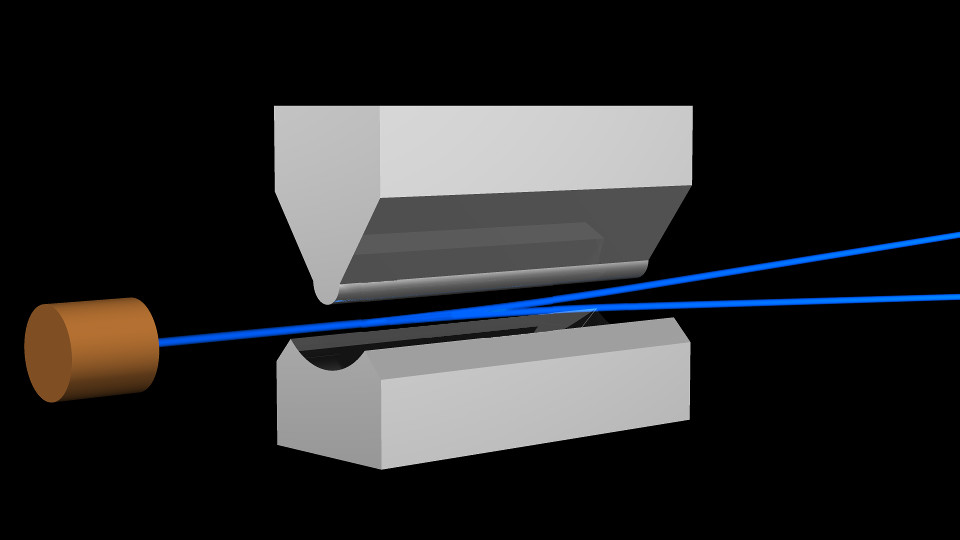
\includegraphics[width=\hsize]{graphics/sterngerlach.jpg}
\caption{Schematische Darstellung des Experimentes von Stern und
Gerlach: ein Strahl von Silber-Atomen wird durch ein inhomegenes
Magnetfeld in zwei Strahlen aufgeteilt.
\label{skript:sterngerlachimage}}
\end{figure}
Der Drehimpuls eines Elektrons in einem Atom "aussert sich ein einem
magnetischen Dipolmoment vom Betrag
\[
\frac{\hbar em}{m_ec}.
\]
In einem inhomogenen Magnetfeld erf"ahrt ein Teilchen mit einem magnetischen
Moment eine von der Orientierung des magnetischen Dipolmomentes 
abh"angige Kraft.
Ein ihomogenes Magnetfeld sollte also
einen Strahl aus solchen Teilchen in mehrere Teilstrahlen
aufgeteilen, einen f"ur jeden m"oglichen Drehimpulszustand.

Dieses Experiment ist erstmals 1922 von Otto Stern und Walther Gerlach
mit einem Strahl von Silber-Atomen durchgef"uhrt
\index{Stern-Gerlach!Versuch von}
(Abbildung~\ref{skript:sterngerlachimage}).
Sie erwarteten die Aufspaltung in drei Teilstrahlen, die den
Werten $m=-1$, $m=0$ und $m=1$ entsprechen.
Beobachtet wurden aber nur zwei Strahlen, und vermuteten daher, dass
der Zustand $m=0$ fehle.

Erst 1925 wurde durch Goudsmith und Uhlenbeck postuliert, dass Elektronen
einen Eigendrehimpuls haben, der aber nur zwei Werte annehmen darf.
Die zugeh"origen Quantenzahlen mussten daher die Werte $l=\frac12$ und
$m=\frac12$ haben.
Es bestand aber immer noch die M"oglichkeit, dass die Aufspaltung
in nur zwei Teilstrahlen mit einem noch nicht verstandenen quantenmechanischen
Effekt in den doch recht komplizierten Silberatomen (Ordnungszahl 47)
erkl"art werden k"onnte.
Diese M"oglichkeit schlossen Experimente an Wasserstoffatomen
von Phipps und Taylor 1927 aus, die auch nur eine Aufspaltung
in zwei Strahlen zeigten.
Das Wasserstoffatom aus nur einem einzigen Eletron und einem Proton
ist sehr viel einfacher gebaut, es kann mit den Grundlagen
der Quantenmechanik bereits vollst"andig berechnet werden,
man darf annehmen, dass man das Wasserstoffatom versteht, und
schliessen, dass die Aufspaltung durch Spin verursacht wird.

%
% XXX man sollte von der zweiwertigkeit ausgehen, und am Schluss
% XXX erkennen, dass dieser Spin die gleichen Vertauschungsregeln
% XXX beinhaltet wie ein Drehimpuls
%
\section{Spin}
\rhead{Spin}
\begin{figure}
\centering
\includegraphics{graphics/spin-2.pdf}
\caption{Termschema f"ur die "Uberg"ange im Natrium-Atom, die zur gelben
Doppellinie (D-Linie) f"uhren.
\label{skript:natriumdlinie}}
\end{figure}%
Die Experimente zeigen also , dass Elektronen sich verhalten, als k"onnten
sie trotz ihrer punktf"ormigen Geometrie rotieren.
Ein Elektron tr"agt also nicht nur seinen ganzzahligen Bahndrehimpuls,
der mit Hilfe der Drehimpulsoperatoren aus Kapitel~\ref{chapter:drehimpuls}
verstanden werden kann, sondern auch noch den halbzahligen Spin.

Bei "Uberg"angen zwischen Energiezust"anden muss auch der Gesamtdrehimpuls
aus Bahndrehimpuls uns Spin erhalten bleiben.
Da Photonen ebenfalls einen Drehimpuls in Form zirkul"arer Polarisierung 
haben, muss ein "Ubergang den Gesamtdrehimpuls des Atoms immer um genau
eine Drehimpulseinheit $\hbar$ "andern.
Der Elektronen-Spin stellt einen zus"atzlichen Freiheitsgrad dar, der die
Zahl der "Uberg"ange vermehrt.
Abbildung~\ref{skript:natriumdlinie} ist das (vereinfachte) Termschema f"ur 
Natrium, es zeigt zwei "Uberg"ange aus einem Zustand mit $l=1$ in einen
Zustand mit $l=0$ aus Zust"anden, die sich nur in der Orientierung
des Spins gegen"uber dem Bahndrehimpuls unterscheiden. 
Im Magnetfeld des Bahndrehimpuls entsteht eine Aufspaltung, die sich
in einer Aufspaltung der gelben Linie des Natriums "aussert.

%Es ist zwar nicht m"oglich, mit Hilfe der Drehimpulsoperatoren
%aus Kapitel~\ref{chapter:drehimpuls}
%dem Elektron einen Eigendrehimpuls zuzuteilen.
%Trotzdem kann man feststellen, dass im Elektron zus"atzlicher
%Drehimpuls stecken muss, denn gew"ohnlicher Drehimpuls kann verschwinden,
%da der Drehimpuls erhalten ist, muss er in das Elektron "ubergegangen
%sein.

Wir schliessen daraus, dass es einen Operator $\vec S$ gibt, der sich
genau so verh"alt wie ein Drehimpulsoperator, allerdings wirkt er nicht
auf die Ortskoordinaten.
Der Operator $\vec S$ heisst der Spin eines Elektrons.
\index{Elektronspin}%
Experimentell weiss man auch, dass Elektronen nur zwei verschiedene
Spinzust"ande haben k"onnen, was bedeutet, dass sich $\vec S$ wie ein
Drehimpulsoperator auf Zustandsvektoren mit $l=\frac12$ verh"alt.
Der Spin-Operator muss auf einen zweidimensionalen Hilbertraum
wirken, die Komponenten des Spin-Operators m"ussen also hermitesche
$2\times 2$-Matrizen sein, die die Vertauschungsrelationen eines
Drehimpulsoperators erf"ullen.

Die Matrizen $I$, $J$ und $K$ in (\ref{skript:komplex:definitionIJK}) haben
algebraische Eigenschaften, die nahe an dem sind, was wir suchen,
allerdings sind sie nicht hermitesch.
Multiplizieren wir sie mit $i$, erhalten wir die hermiteschen Matrizen
\begin{align}
\sigma_1
&=
\begin{pmatrix}
0&1\\1&0
\end{pmatrix}
&
\sigma_2
&=
\begin{pmatrix}
0&-i\\i&0
\end{pmatrix}
&
\sigma_3
&=
\begin{pmatrix}
1&0\\0&-1
\end{pmatrix}
\label{spin:paulimatrizen}
\end{align}
\index{Pauli-Matrizen}%
die auch {\em Pauli-Matrizen} genannt werden.
Diese Matrizen haben die folgenden Multiplikationseigenschaften:
\begin{align*}
%\sigma_1^2
%=
%\sigma_2^2
%=
%\sigma_3^2
%&=E,
%&
\sigma_1\sigma_2
&=
\begin{pmatrix} i&0\\0&-i \end{pmatrix} = i\sigma_3,
&
\sigma_2\sigma_3
&=
\begin{pmatrix} 0&i\\i&0 \end{pmatrix} = i\sigma_1,
&
\sigma_3\sigma_1
&=
\begin{pmatrix} 0&1\\-1&0 \end{pmatrix} = i\sigma_2,
\\
%&&
\sigma_2\sigma_1
&=
\begin{pmatrix} -i&0\\0&i \end{pmatrix} = -i\sigma_3,
&
\sigma_3\sigma_2
&=
\begin{pmatrix} 0&-i\\-i&0 \end{pmatrix} = -i\sigma_1,
&
\sigma_1\sigma_3
&=
\begin{pmatrix} 0&-1\\1&0 \end{pmatrix} = -i\sigma_2.
\end{align*}
\index{Pauli-Matrizen!Vertauschungsrelationen}%
Die Vertauschungsrelationen sind
\begin{align*}
[\sigma_1,\sigma_2]
&=
2i\sigma_3,
&
[\sigma_2,\sigma_3]
&=
2i\sigma_1,
&
[\sigma_3,\sigma_1]
&=
2i\sigma_2.
\end{align*}
Dies sind bis auf einen Faktor $\hbar/2$ die Vertauschungsrelationen,
die wir von einem Drehimpulsoperator erwarten,
daher k"onnen wir den Vektoroperator
\begin{equation}
\vec S=\frac{\hbar}2\vec\sigma
=
\frac{\hbar}2\begin{pmatrix}\sigma_1\\\sigma_2\\\sigma_3\end{pmatrix}
\label{spin:vektoroperator}
\end{equation}
als Spin-Operator verwenden.
\index{Spin-Operator}%
Der Betrag des Spin-Operators ist
\begin{align*}
\vec S^2
=
\frac{\hbar}{4}(\sigma_1^2+\sigma_2^2+\sigma_3^2)=\hbar^2\frac12\frac32E.
\end{align*}
Die Standardbasisvektoren sind Eigenvektoren sowohl von $\vec S^3$ wie
auch von $S_3$.
Wir bezeichnen sie daher auch $|\uparrow\rangle=e_1$ und
$|\downarrow\rangle=e_2$, es gilt:
\begin{align*}
\vec S^2\,|\uparrow\rangle&=\frac{3\hbar}4\,|\uparrow\rangle
&
\vec S^2\,|\downarrow\rangle&=\frac{3\hbar}4\,|\downarrow\rangle
\\
S_3\,|\uparrow\rangle&=\frac{\hbar}{2}\,|\uparrow\rangle
&
S_3\,|\downarrow\rangle&=-\frac{\hbar}{2}\,|\downarrow\rangle
\end{align*}

Die Auf- und Absteigeoperatoren f"ur den Spin sind
\index{Spin!Auf- und Absteigeoperatoren}%
\begin{align}
S_+
&=
S_1+iS_2
=
\frac{\hbar}2
(\sigma_1+i\sigma_2)
=
\frac{\hbar}2
\begin{pmatrix} 0&1+1\\1-1&0 \end{pmatrix}
=\hbar\begin{pmatrix}0&1\\0&0\end{pmatrix},
\\
S_-
&=
S_1-iS_2
=
\hbar\begin{pmatrix} 0&0\\1&0\end{pmatrix},
\\
S_+S_-+S_-S_+
&=
\hbar^2E,
\end{align}
genau wie f"ur den Operator $\vec L$.
Auf den Standardbasisvektoren wirken diese Operatoren wie
\begin{align*}
S_+\,|\uparrow\rangle&=0,
&
S_-\,|\uparrow\rangle&=\hbar\,|\downarrow\rangle,
\\
S_+\,|\downarrow\rangle&=\hbar\,|\uparrow\rangle,
&
S_-\,|\downarrow\rangle&=0.
\end{align*}
$S_+$ erh"oht also den Spin in $z$-Richtung, $S_-$ erniedrigt ihn.

\section{Spin im Magnetfeld}
\rhead{Spin im Magnetfeld}
Der Spin manifestiert sich durch seine Wechselwirkung mit einem
externen Magnetfeld.
Diese Wechselwirkung kann durch einen zus"atzlichen Term im
Hamilton-Operator modelliert werden.
Die Wechselwirkung eines magnetischen Dipolmoments mit einem
Magnetfeld $\vec B$ wird durch das Skalarprodukt gegeben,
der Hamilton-Operator, der sie ber"ucksichtigt, ist daher
\index{Spin!im Magnetfeld}%
% XXX Masseinheit: SI?
\[
H=H_0 + \frac{e}{m_ec}\vec S\cdot\vec B.
\]
Darin ist $H_0$ der Hamilton-Operator ohne die Wechselwirkung 
zwischen Spin und Magnetfeld.

Wir k"onnen die St"orungstheorie verwenden, um den Einfluss eines
Magnetfeldes auf den Spin abzusch"atzen.
Da der ungest"orte Operator $H_0$ den Spin nicht enth"alt, gibt
es entartete Eigenzust"ande
$|\uparrow\rangle$ und $|\downarrow\rangle$
zu verschiedenen Spins, die aber sonst in allen Quantenzahlen
"ubereinstimmen.
Sie sind aber Eigenzust"ande des Spin-Magnetfeld-Operators
$\vec S\cdot \vec B$, so dass wir die St"orungstheorie anwenden
k"onnen.

In erster N"aherung sagt die St"orungstheorie, dass die Spin-Zust"ande
durch die St"orungstheorie nicht gemischt werden.
Nur die Energien werden sich "andern, und die "Anderung in 
Abh"angigkeit vom Magnetfeld k"onnen wir berechnen.

Wir nehmen an, dass das Magnetfeld nur eine $z$-Komponente $B_z$ hat,
dieses ist der St"orungsparameter.
Der Operator $H_1$ ist in dieser Basis durch die Matrix
\[
H_1=
\frac{\hbar e}{2m_ec}
\begin{pmatrix}
1&0\\
0&-1
\end{pmatrix}
\]
gegeben.
Die St"orungstheorie liefert f"ur den linearen Koeffizienten von $B_z$
der Energie
\begin{align*}
E_\downarrow^{(1)}
&=
\langle \downarrow|\, H_1 \,|\downarrow\rangle
=\frac{\hbar e}{2m_e c}
&
E_\uparrow^{(1)}
&=
\langle \uparrow|\, H_1 \,|\uparrow\rangle
=-\frac{\hbar e}{2m_e c}
\end{align*}
Durch die St"orung werden die beiden Spin-Niveaus aufgespalten
in zwei Niveaus, deren Energie sich um
\[
\frac{\hbar e}{m_e c}B_z
\]
unterscheidet.

\section{Spin und Statistik}
\rhead{Spin und Statistik}
\index{Spin!und Statistik}%
Die Theorie sagt aus, dass ein Teilchen nur einen totalen Spin haben kann,
der ein Vielfaches von $\frac12$ ist. Tats"achlich gibt es Teilchen
ganz ohne Spin, die $\pi$-Mesonen geh"oren dazu, aber auch das Higgs-Boson.
Elektronen, Protonen und Neutronen haben Spin $\frac12$. 
Atomkerne setzen sich aus vielen Protonen und Neutronen zusammen, ihr
Spin kann daher viel h"oher sein. Im Grundzustand haben jedoch auch
sie einen kleinen Spin.

\subsection{Austauschoperator}
Ein einzelnes Teilchen hat in der Ortsdarstellung als Zustand
eine Wellenfunktion, die von den Ortskoordinaten und der Zeit abh"angt,
sie hat zwei Komponenten, eine f"ur jeden m"oglichen Spinzustand.
Wir k"onnten schreiben
\begin{equation}
|\psi\rangle
=
\begin{pmatrix}
\psi_\uparrow(x,y,z,t)\\
\psi_\downarrow(x,y,z,t)
\end{pmatrix}
\label{spin:vector}
\end{equation}
Statt die beiden m"oglichen Spinzust"ande durch einen Index zu unterscheiden,
k"onnten wir sie auch als Argumente der Wellenfunktion schreiben, also
als $\psi(x,y,z,t,s)$, wobei $s$ die Spinvariable ist. Der Zusammenhang
mit den Komponenten in (\ref{spin:vector}) ist
\[
\psi_\uparrow(x,y,z,t)
=
\psi(x,y,z,t,\uparrow)
\qquad\text{und}\qquad
\psi_\downarrow(x,y,z,t)
=
\psi(x,y,z,t,\downarrow).
\]
Wie sieht die Wellenfunktion eines Systems mit zwei Teilchen aus?
In die Wellenfunktion dieses Systems m"ussen die Koordinaten
$(x_1,y_1,z_1)$ und $(x_2,y_2,z_2)$ beider Teilchen eingehen, 
sowie die beiden Spins. Wir k"onnen die beiden Spins wieder als
Koordinaten einer Wellenfunktion
\[
|\psi_2\rangle
=
\psi_2(x_1,y_1,z_1,s_1,x_2,y_2,z_2,s_2,t)
\]
betrachten.
Elementarteilchen sind nicht unterscheidbar. Das bedeutet, dass sich
physikalisch nichts "andern darf, wenn wir die Koordinaten der beiden
Teilchen in $\psi_2$ vertauschen. Alle daraus berechneten physikalischen
Gr"ossen m"ussen gleich bleiben.

Wir k"onnen die Operation, die die Koordinaten vertauscht, also
Operator $A$ betrachten:
\index{Austauschoperator}%
\[
|\psi_2\rangle
=
\psi_2(x_1,y_1,z_1,s_1,x_2,y_2,z_2,s_2,t)
\mapsto
A|\psi_2\rangle
=
\psi_2(x_2,y_2,z_2,s_2,x_1,y_1,z_1,s_1,t)
\]
$A$ ist ein selbstadjungierter Operator.
Wendet man den Operator zweimal an, bleibt der Zustand unver"andert.
Der Operator $A$ erf"ullt also die Gleichung $A^2=\operatorname{id}$,
insbesondere kann $A$ nur Eigenwerte $\pm 1$ haben.
Ein Eigenzustand von $A$ erf"ullt also immer eine der beiden 
Gleichungen
\begin{align*}
A|\psi_2\rangle &= |\psi_2\rangle
\tag{symmetrisch}
\\
A|\psi_2\rangle &=-|\psi_2\rangle
\tag{antisymmetrisch}
\end{align*}
Wir k"onnen auch aus einem beliebigen Zustandsvektor $|\psi\rangle$
Eigenvektoren zu jedem $A$ bauen, indem wir
\begin{align*}
|\psi_\text{symmetrisch}\rangle
&=
\frac1{\sqrt{2}}(|\psi\rangle + A\,|\psi\rangle)
&
|\psi_\text{antisymmetrisch}\rangle
&=
\frac1{\sqrt{2}}(|\psi\rangle - A\,|\psi\rangle)
\end{align*}
bilden.

Wenn die beiden Teilchen nicht unterscheidbar sind, dann darf sich
die Energie nicht "andern, wenn die beiden Teilchen vertauscht
werden. Der Hamilton-Operator $H$ muss also mit $A$ vertauschen:
$[H,A]=0$. Wir k"onnen die Eigenzust"ande von $H$ also immer so
w"ahlen, dass sie auch Eigenzust"ande von $A$ sind.

Wenn $|\psi\rangle$ ein Eigenzustand von $H$ ist, dann muss auch
$|\psi_{\text{symmetrisch}}\rangle$ und
$|\psi_{\text{antisymmetrisch}}\rangle$ ein Eigenvektor sein.

\subsection{Pauli-Prinzip}
Die Operator $H$ und $A$ erlaubten uns nicht zu entscheiden, welcher
der beiden Zust"ande $|\psi_{\text{symmetrisch}}\rangle$ und
$|\psi_{\text{antisymmetrisch}}\rangle$ in der Natur tats"achlich
vorkommt.
Experimentell hat man festgestellt, dass Teilchen mit halbzahligem
Spin, sogenannte Fermionen, nur mit einer antisymmetrischen
\index{Fermion}%
Wellenfunktion vorkommen k"onnen, w"ahrend Teilchen mit
ganzzahligem Spin, sogenannte Bosonen, nur mit einer symmetrischen
Wellenfunktion auftreten.
\index{Boson}

Wenn zwei Fermionen keine Wechselwirkung haben, dann k"onnen wir
aus zwei Wellenfunktionen
$\psi(x_1,y_1,z_1,s_1,t)$
und
$\psi(x_2,y_2,z_2,s_2,t)$
f"ur Fermionen eine antisymmetrische Wellenfunktion
\[
\psi_2(x_1,y_1,z_1,x_2,y_2,z_2,s_1,s_2,t)
=
\psi(x_1,y_1,z_1,s_1,t)
\psi(x_2,y_2,z_2,s_2,t).
\]
f"ur das Gesamtsystem bauen.
Wenn die beiden Fermionen den gleichen Spin haben, ist die
Funktion $\psi_2$ symmetrisch, kann also nicht die Wellenfunktion
eines Paares von Fermionen sein. 
Daraus leiten wir das Pauli-Prinzip ab:

\begin{satz}[Pauli-Prinzip]
Zwei Fermionen k"onnen nicht in einem Zustand sein, in dem alle
Quantenzahlen "ubereinstimmen.
\end{satz}
Zwei Fermionen m"ussen sich also in mindestens einer Quantenzahl
unterscheiden.
Zwei Elektronen k"onnen in einem Atom nur dann die gleichen
Energie- und Drehimpuls-Quantenzahlen haben, wenn sie sich im
Spin unterscheiden.

\subsection{Periodensystem}
\index{Periodensystem}%
Die Elektronen in einem Atom sind nicht voneinander unabh"angig,
jedes Elektron bewegt sich in einem Potential, welches vom Kern
und allen anderen Elektronen zusammen erzeugt wird.
In erster N"aherung k"onnen wir annehmen, dass alle Elektronen
das gleiche Potential sp"uren.
Selbst in dieser vereinfachten Situation schr"ankt das Pauli-Prinzip
die m"oglichen Elektronenzust"ande in einem Atom stark ein.
Keine zwei Elektronen k"onnen die gleichen Quantenzahlen f"ur
den Drehimpuls und den Spin haben.

Im Grundzustand werden in dieser N"aherung die Elektronen die Zust"ande
mit minimaler Energie ausw"ahlen.
In unserer Untersuchung des Wasserstoffatoms hat gezeigt, dass in
erster N"aherung die Energie nur von der Quantenzahlen $n$ abh"angt,
nicht von $l$, $m$ oder vom Spin, diese Energieniveaus sind entartet.

Die verschiedenen Drehimpulszust"ande werden durch die Spin-Bahn-Kopplung
aufgespalten (siehe Abbildung~\ref{skript:wasserstoffaufspaltung}).
Man kann sie sich als eine Wechselwirkung des vom Spin erzeugten
Magnetischen Momentes mit dem von der Bahnbewegung verursachten
Magnetfeld vorstellen.
Relativistische Effekte, die mit der Quantenelektrodynamik vollst"andig
verstanden werden k"onnen, sorgen daf"ur, dass in realen Atomen
die verschiedenen $m$-Werte zu leicht verschiedenen Energien f"uhren.
Die Wechselwirkung der verschiedenen Elektronenspins untereinander
spalten auch die letzten Niveaus noch auf.
Insgesamt k"onnen wir also davon ausgehen, dass alle Energieniveaus
verschieden sind.

Je gr"osser die Ladung des Kernes ist, desto mehr der m"oglichen
Elektronenzust"ande werden von Elektronen tats"achlich besetzt.
Die chemischen Eigenschaften eines Atoms h"angen davon ab, welche
Energie n"otig ist, ein Elektron zu entfernen oder hinzuzf"ugen.
Je nach den Quantenzahlen der Elektronen mit der gr"ossten Energie
werden sich die chemischen Eigenschaften "andern.
Man kann also erwarten, dass die Elemente "ahnliche Eigenschaften
zeigen, wenn ihre "aussersten Elektronen die gleichen $l$ und $m$
Quantenzahlen haben.

Das niedrigste Energieniveau ist $n=0$, in diesem Niveau gibt es
keine Zust"ande mit Drehimpuls $l\ne 0$. Es bleiben nur die
beiden Spin-Zust"ande, es gibt also nur zwei Atome, bei denen nur
die Zust"ande f"ur $n=0$ besetzt sind:
\begin{center}
\includegraphics{graphics/periodensystem-1.pdf}
\end{center}
Die Zust"ande der "aussersten Elektronen sind also solche mit
$l=0$, in dieser und den folgenden Tabelle sind sie rot
hinterlegt.
In Abschnitt~\ref{section:orbitale} haben wir diese Zust"ande unter
dem Namen s-Orbitale kennengelernt.

Wenn man mehr Elektronen hat, k"onnen auch die Zust"ande mit $n=1$ 
besetzt werden.
Hier gibt es insgesamt drei zus"atzliche Zust"ande mit Drehimpuls $l=1$,
die im Abschnitt~\ref{section:orbitale} p-Orbitale genannt wurden,
jeder mit zwei m"oglichen Spinzust"anden.
Die sechs Zust"ande f"ur $l=1$, die in der folgenden Tabelle 
gr"un hervorgehoben sind.
Es ist energetisch g"unstiger, als erstes einen der
Drehimpulszust"ande $l=0$ zu besetzen, und erst dann die Drehimpulszust"ande
mit $l=1$.
\begin{center}
\includegraphics{graphics/periodensystem-2.pdf}
\end{center}
Die Niveaus mit $l=2$
sind energetisch ung"unstiger
und kommen erst nach
den Niveaus f"ur $n=3$ und kleine Drehimpulse.

F"ur $n>2$ k"onnen die Niveaus mit $l=2$, die d-Orbitale, besetzt werden.
Zusammen mit
dem Spin gibt es zehn zus"atzliche Niveaus, die in der folgenden Tabelle
blau hervorgehoben sind.
\begin{center}
\includegraphics{graphics/periodensystem-3.pdf}
\end{center}

F"ur $n>4$ k"onnen schliesslich sogar die Niveaus $l=3$, die
f-Orbitale, besetzt werden.
Da es sieben Drehimpulszust"ande mit $l=3$ gibt, gibt es zusammen mit den
Spinzust"anden also vierzehn zus"atzliche Zust"ande, die in
der Tabelle gelb hervorgehoben sind
\begin{center}
\includegraphics[width=\hsize]{graphics/periodensystem-4.pdf}
\end{center}
Nat"urlich k"onnte man diese Tabelle noch viel weiter fortsetzen,
solange es aber keine so schweren Atomkerne gibt, sind solche Atome
nicht realisierbar.


\chapter{Festk"orper\label{chapter:festkoerper}}
\lhead{Festk"orper}
\rhead{}
Festk"orper sind aus vielen Atomen zusammengesetzte Quantensysteme.
Im Gegensatz zu einer Fl"ussigkeit sind jedoch die Atomkerne mehr
oder weniger unverr"uckbar in einem Gitter angeordnet.
Bei elektrischen Leitern ist ein Teil der Elektronen weitgehend frei
beweglich.
Nat"urlich ist die Gitterstruktur ebenfalls die Folge der Interaktionen
zwischen den Elektronen, doch f"ur unsere Untersuchungen k"onnen wir
die Entstehung der Gitterstruktur vernachl"assigen, es einfach als
gegeben ansehen, und nur noch die Eigenschaften der frei beweglichen
Elektronen studieren.
Diese Elektronen bewegen sich in dem periodischen Potential, das von
den Atomkernen des Gitters erzeugt wird.
Jeder Atomkern erzeugt einen Potentialtopf, in dem eines oder mehrere
Elektronen gefangen sind.
Bleiben nach der Besetzung dieser lokalisierten Zust"ande noch
Elektronen "ubrig, dann haben diese mehr Energie als die Schwellen zwischen
den Potentialt"opfen hoch sind, aber nicht gen"ugend Energie, um
aus dem Festk"orper auszutreten.
Diese wie auch die Elektronen, die mit nur wenig Anregungsenergie
in einen ausgedehnten Zustand versetzt werden k"onnen, interessieren
uns in diesem Kapitel.

\section{Fermikugel}
In erster N"aherung betrachen wir den Festk"orper als einen
sehr grossen Potenialkasten, aus dem die Elektronen nicht austreten
k"onnen.
Die gebundenen Elektronen vernachl"assigen wir, sie tragen zu
Leitungsph"anomenen nichts bei.

\section{Kristalle}
\subsection{Symmetrien}
Kristalle sind Festk"orper, deren Atomkerne in einem regelm"assigen
Gitter angeordnet sind.
Im einfachsten Fall gibt es eine Menge 
$ \Gamma  \subset \mathbb R^3 $
so, dass eine Verschiebung aller Atomkerne um einen Vektor aus $\Gamma$
den Festk"orper nicht "andert.
Wir k"onnen die Verschiebung um einen Vektor $\vec v\in\Gamma$ als
Operator $T_{\vec v}$ auf dem Hilbertraum der Zustandsvektoren
betrachten:
\[
(T_{\vec v}\psi)(x)=\psi(x-\vec v).
\]
Der Hamilton-Operator "andert sich nicht, wenn man die Atomkerne um
einen Vektor $\vec v\in\Gamma$ verschiebt.
Also muss der Hamilton-Operator mit allen Translationen $T_{\vec v}$ 
vertauschen.
Es gibt also eine Basis von Eigenvektoren von $H$, welche auch
Eigenvektoren aller Operatoren $T_{\vec v}$ sind, f"ur jeden Vektor
$\vec v\in\Gamma$.

Die Menge $\Gamma$ hat noch etwas mehr Struktur als wir bisher
verwendet haben.
Wenn zwei Vektoren $\vec v_1,\vec v_2\in\Gamma$ sind, dann muss
auch deren Summe $\vec v_1+\vec v_3\in\Gamma$ sein.
Man nennt $\Gamma$ eine Gruppe.

Ausserdem ist es nicht n"otig, sich auf die Translationen $\Gamma$
zu beschr"anken.
Der Festk"orper kann durchaus noch weitere Symmetrien haben, zum
Beispiel Drehungen oder Spiegelungen.
Auch diese Symmetrien k"onnen als Operatoren beschrieben
werden, die auf den Zustandsvektoren wirken.
Die Menge aller Symmetrietransformationen nennen wir $G$.
Die Menge $G$ bildet ebenfalls eine Gruppe: jeder Verkn"upfung von
Symmetrieoperationen ist wieder eine Symmetrieoperation, und die
Inverse einer Symmetrieoperation ist ebenfalls eine Symmetrieoperation.
Die m"oglichen Symmetriegruppen von Kristallen sind vollst"andig
klassifiziert worden.

Eine Transformation darf die Norm der Zustandsvektoren nicht "andern,
die Transformationen in $G$ sind also unit"are Operatoren,
$U^*U=UU^*=\operatorname{id}$ f"ur alle $U\in G$.
Die Eigenwerte von Transformationen in $G$ sind daher alle in $U(1)$.
Die Transformationen einer Eigenfunktion von $H$ und allen Operatoren in $G$
"andert eine Wellenfunktion als h"ochstens um einen Phasenfaktor.
Zu jedem Operator $U\in G$ gibt es also einen Eigenwert $\chi(U)\in U(1)$,
und die Zusammensetzung von Operatoren muss mit der Abbildung $\chi$
vertauschen, d.~h.
\[
\begin{aligned}
\chi(UV)&=\chi(U)\chi(V)&&U,V\in G\\
\chi(U^*)&=\bar\chi(U)&&U\in G
\end{aligned}
\]
Man nennt eine solche Abbildung einen Darstellung der Gruppe $G$.
Auch die Darstellungen der Gruppen $G$ sind vollst"andig klassifiziert
worden.

\subsection{Periodisches Potential}
Als Beispiel betrachten wir einen eindimensionalen Kristall, dessen
Atomkerne an den Stellen $an$, $n\in\mathbb Z$ platziert sind.
$a$ ist der Abstand zwischen den Atomkernen.
Statt Coulomb-Potentials verwenden wir ein schmalen Potentialtopf.
Dieser Kristall hat einerseits die Translationssymmetrie $T_{an}$ um
ganzzahlige Vielfache von $a$, und andererseits eine Spiegelung $S$.
Die Translationen und die Verschiebungen vertauschen nicht, es gilt
\[
T_{na}S=ST_{-na}.
\]
Da die Spiegelung $S^2=\operatorname{id}$ erf"ullt, kann sie nur
Eigenwerte $1$ oder $-1$ haben.
Wenden wir darauf $\chi$ an, finden wir
\[
\chi(a)^n\chi(S)=\chi(S)\bar\chi(a)^n
\qquad \Rightarrow \qquad
\chi(a)^2=1
\]

Wir suchen also Zustandsvektoren, welche Eigenwerte der
Symmetrieoperatoren sind.

\section{Valenz- und Leitungsband}




\begin{appendices}
\chapter{Anhang: Komplexe Zahlen}
\lhead{Komplexe Zahlen}
\rhead{}
Der mathematische Formalismus der Quantenmechanik kann nicht ohne komplexe
Zahlen auskommen.
Leonhard Euler sah die Zahlen $\sqrt{-1}$ noch als imagin"ar an,
also als ohne Gegenst"uck in der realen Welt.
Elektroingenieure verwenden komplexe Zahlen mit grossem Erfolg in ihren
Anwendungen, sie spielen aber vor allem die Rolle eines praktischen
Werkzeugs. Die Regeln, mit denen am Schluss solcher Rechnungen sichergestellt
wird, dass die Resultate reell sind zeigt ausserdem, dass man alles auch
ohne komplexe Zahlen durchrechnen k"onnte, wenn auch wesentlich weniger
elegant.

In der Quantenmechanik geht es aber nicht mehr ohne komplexe Zahlen,
die physikalischen Gr"ossen selbst sind komplex. Es gibt zwar auch
hier wieder Regeln, die sicherstellen, dass Messresultate reell sind
(Operatoren m"ussen selbstadjungiert sein), aber sie erlauben nicht,
die ganze Quantenmechanik auf eine Art zu beschreiben, die ohne komplexe
Zahlen auskommt.

\section{Der K"orper $\mathbb C$ der komplexen Zahlen}
In den reellen Zahlen $\mathbb R$ k"onnen alle Grundoperationen ausgef"uhrt
werden, es ist jedoch nicht m"oglich, die Quadratwurzeln aus negativen
Zahlen zu ziehen. Eine analoge Situation trifft man schon viel fr"uher.
In den nat"urlichen Zahlen $\mathbb N$ kann man zwar addieren und
multiplizieren, aber nicht subtrahieren.
F"ugt man die negativen Zahlen hinzu erh"alt man eine Menge $\mathbb Z$,
in der die Subtraktion uneingeschr"ankt m"oglich ist. Division ist aber
immer noch nur f"ur spezielle Divisoren m"oglich. F"ugt man jedoch die
Br"uche zu $\mathbb Z$ hinzu, erh"alt man die Menge der rationalen Zahlen
$\mathbb Q$, in der Division uneingeschr"ankt m"oglich ist.
Doch auch $\mathbb Q$ ist nicht vollst"andig, die Zahl $\sqrt{2}$ ist
keine rationale Zahl. Nat"urlich kann man $\sqrt{2}$ durch eine
Folge von Br"uchen $r_n\in\mathbb Q$ approximieren, doch der Grenzwert
dieser Folge $\lim_{n\to\infty}r_n=\sqrt{2}$ ist nicht in $\mathbb Q$.
F"ugt man jedoch alle Grenzwerte von konvergenten Folgen zu $\mathbb Q$
hinzu, erh"alt man die Menge $\mathbb R$ der reellen Zahlen, in der
auch beliebige Wurzeln von positiven Zahlen gezogen werden k"onnen,
oder andere Grenzwerte wie $\pi$, $e$, die Werte von $\sin x$ und $\cos x$
und weitere.

\subsection{Grundoperationen f"ur die komplexen Zahlen}
Nach analogem Muster k"onnen wir auch $\mathbb R$ erweitern, so dass auch
die Wurzeln aus negativen Zahlen bestimmt werden k"onnen. Es reicht
sogar, nur die Wurzel von $-1$ hinzuzuf"ugen, denn jede andere Wurzel
einer negativen Zahl ist $\sqrt{-a}=\sqrt{-1}\cdot\sqrt{\mathstrut a}$.
Euler hat die Bezeichnung $i=\sqrt{-1}$ f"ur die imagin"are Einheit eingef"uhrt.
Es gilt nat"urlich $i^2=-1$.

\begin{definition}
Die Menge $\mathbb C=\{a+bi\,|\,a,b\in\mathbb R\}$ heisst die Menge der
komplexen Zahlen. Die komplexe Zahl $z=a+bi$ hat
Realteil $\operatorname{Re}z=a$ und Imagin"arteil $\operatorname{Im}z=b$.
Die Rechenoperationen sind so zu verstehen, die Rechenregeln
der Algebra erhalten bleiben\footnote{Man nennt dies das Permanenz-Prinzip}.
\end{definition}

Die Rechenoperationen folgen aus der Definition:
\begin{align*}
(a+bi)+(c+di)&=(a+c)+(b+d)i\\
(a+bi)(c+di)&=ac-i^2bd+(ad+bc)i=ac-bd+(ad+bc)i
\end{align*}
Die Division stellt noch ein Problem dar. Hier hilft das Konzept der
konjugiert komplexen Zahl.

\begin{definition}
Die Zahl $\bar z=a-bi$ heisst die zu $z=a+bi$ konjugiert komplexe Zahl.
\end{definition}

Zun"achst kann man mit der konjugiert komplexen Zahl den Betrag einer
komplexen Zahl definieren:
\[
z\bar z=(a+bi)(a-bi)=a^2+abi-abi-i^2b^2=a^2+b^2\qquad\Rightarrow\qquad
|z|^2=z\bar z.
\]
Andererseits kann man damit auch komplexe Br"uche berechnen, indem man
mit der konjugiert komplexen Zahl des Nenners erweitert:
\begin{align*}
\frac{a+bi}{c+di}&=
\frac{a+bi}{c+di}
\cdot
\frac{c-di}{c-di}=\frac{ac-bd+(ad+bd)i}{c^2+d^2}
\end{align*}
Die komplexen Zahlen k"onnen in einer Ebene visualisert werden: 
Realteil und Imagin"arteil werden entlang orthogonaler Achsen abgetragen.
Die Punkte $(x,y)$ der $x$-$y$-Ebene entsprechen also der komplexen Zahl
$x+yi$ der komplexen Zahlenebene.

\subsection{Polardarstellung}
Die Darstellung der komplexen Zahlen als Punkte einer Ebene suggeriert
auch eine alternative Schreibweise.
Ein Punkt $z$ der komplexen Ebene kann auch charakterisiert werden mit Hilfe von
Polarkoordinaten, also durch seine Entfernung $r=|z|$ vom Nullpunkt,
und durch Polarwinkel zwischen der reellen Achse und der Richtung
zur komplexen Zahl. Der Polarwinkel heisst auch Argument $\operatorname{arg}z$,
und es gilt
\[
\tan\operatorname{arg}z=\frac{\operatorname{Re}z}{\operatorname{Im}z}.
\]
Die Multiplikation von komplexen Zahlen bekommt in der Polardarstellung
eine besondere Interpretation:
\begin{align*}
z_1z_2
&=
(r_1\cos\varphi_1+ir_1\sin\varphi_1) (r_2\cos\varphi_2+ir_2\sin\varphi_2)
\\
&=
r_1r_2(\cos\varphi_1+i\sin\varphi_1) (\cos\varphi_2+i\sin\varphi_2)
\\
&=
r_1r_2\bigl(
\cos\varphi_1\cos\varphi_2-\sin\varphi_1\sin\varphi_2 +
(\cos\varphi_1\sin\varphi_2+\sin\varphi_1\cos\varphi_2)i\bigr)
\\
&=
r_1r_2(\cos(\varphi_1+\varphi_2)+i\sin(\varphi_1+\varphi_2))
\\
\Rightarrow \operatorname{arg}z_1z_2&=\arg z_1 + \arg z_2
\end{align*}
Die Multiplikation zweier komplexen Zahlen entspricht also der
Multiplikation der Betr"age, und der Addition der Argumente.

Wir versuchen jetzt, die Werte der Exponentialfunktion zu $e^z$ zu
bestimmen.
Die Exponentialgesetze sollten auch weiterhin gelten.
Sei also $z=a+bi$, dann ist
\[
e^z=e^{a+bi}=e^a\cdot e^{bi}.
\]
Die Exponentialfunktion reeller Zahlen ist bereits wohlbekannt, es muss
also nur noch untersucht werden, welche Bedeutung $e^{bi}$ hat.

Betrachten wir die Funktion $f(t)= e^{ti}$. Die Ableitungen von $f$ sind
\begin{align}
f'(t)&=ie^{ti}=if(t)\notag\\
f''(t)&=-f(t).\label{exp-dgl}
\end{align}
Die Funktion $f$ muss also eine L"osung der Differentialgleichung
(\ref{exp-dgl}) sein, welche die Anfangsbedingungen $f(0)=1$ und
$f'(0)=if(0)=i$ erf"ullen muss.
Doch die Differentialgleichung (\ref{exp-dgl}) hat die L"osungen
\[
f(t)=a\cos t+b\sin t.
\]
Setzt man die Anfangsbedingungen ein findet man
\begin{align*}
f(0)&=1&\Rightarrow&&a&=1\\
f'(0)&=1&\Rightarrow&&b&=i,
\end{align*}
so dass wir jetzt $e^{ti}$ ausrechnen k"onnen:
\begin{satz}[Euler]
\begin{align}
e^{it}=\cos t+i\sin t.
\label{euler-formula}
\end{align}
\end{satz}
Mit dieser Formel sind wir jetzt auch in der Lage, den Zusammenhang
zwischen einer komplexen Zahl und ihrem Betrag und Argument sehr pr"agnant
auszudr"ucken:
\[
z=|r|\cdot e^{i\operatorname{arg}z}.
\]

\subsection{Matrixdarstellung der komplexen Zahlen}
Die Algebra der komplexen Zahlen kann man auch als eine Algebra von Matrizen
schreiben. Dazu betrachten wir die Abbildung
\[
\varphi\colon
\mathbb C\to M_2(\mathbb R):
a+bi\mapsto\begin{pmatrix}a&b\\-b&a\end{pmatrix}
\]
Die imagin"are Einheit $i$ wird von $\varphi$ auf die Matrix
\[
\varphi(i)=J=\begin{pmatrix}0&1\\-1&0\end{pmatrix}
\]
abgebildet. Man kann nachrechnen, dass $J^2=-E$, und dass die Rechenregeln
f"ur die komplexen Zahlen durch die Abbildung $\varphi$ in die Rechenregeln
f"ur Matrizen transformiert werden.
Wir illustrieren dies f"ur die Multiplikation:
\begin{align*}
&(a+bi)(c+di)&&\mapsto&
&\begin{pmatrix}a&b\\-b&a\end{pmatrix}
\begin{pmatrix}c&d\\-d&c\end{pmatrix}
\\
&(ac-bd) + i(ad-bc)&&\mapsto&
&=\begin{pmatrix}
ac-bd&ad-bc\\
-ad+bc&ac-bd
\end{pmatrix}
\end{align*}

\section{Komplexe Matrizen}
Die Lineare Algebra im Bachelor wird typischerweise nur in den
reellen Zahlen entwickelt, der einzige untersuchte Vektorraum ist
der Raum $\mathbb R^n$ der reellen $n$-dimensionalen Vektoren.
F"ur die Quantenmechanik ben"otigen wir aber auch Vektoren mit
komplexen Komponenten. Der $n$-dimensionale komplese Vektorraum
$\mathbb C^n$ ist die Menge
\[
\left\{\left.\begin{pmatrix}c_1\\\vdots\\c_n\end{pmatrix}\,\right|
c_i\in\mathbb C\right\},
\]
mit der komponentenweisen Addition und der Multiplikation mit einer
komplexen Zahl. Nichts an der elementaren linearen Algebra hat besondere
Eigenschaften der reellen Zahlen verwendet, die nicht auch die komplexen
Zahlen haben. Der Gauss-Algorithmus, die Konstruktion der Determinanten,
ja sogar der grundlegende Algorithmus zur L"osung des Eigenwertprobems
funktioniert genau gleich auch f"ur komplexe Matrizen. Nur im Bereich
des Skalarproduktes sind minimale Modifikationen notwendig, damit

\subsection{Skalarprodukt f"ur komplexe Vektorr"aume}
In der linearen Algebra im ersten Semester wird das Skalarprodukt
geometrisch mit Hilfe der Projektion eingef"uhrt.
Eine solche Konstruktion ist f"ur komplexe Vektoren nicht m"oglich,
weil es keine anschauliche komplexe Geometrie gibt.

\subsubsection{Komplexes Skalarprodukt}
Um ein komplexes Skalarprodukt zu bekommen, gehen wir daher von den
algebraischen Eingeschaften des Skalarproduktes aus:
\begin{compactenum}
\item Das Skalarprodukt $(u,v)$ von komplexen Vektoren $u$ und $v$ ist linear
in $v$.
\item $(u,u) > 0$ falls $u\ne 0$.
\item Falls $(u,v)\in\mathbb R$, dann ist $(u,v)=(v,u)$.
\end{compactenum}
Diese Eigenschaften m"ussen auch f"ur ein komplexes Skalarprodukt gelten.
Wir zeigen, dass diese Eigenschaften auch ein komplexes Skalarprodukt 
weitgehend festlegt.

Zun"achst stellen wir fest, dass wir nicht erwarten k"onnen, dass
ein Skalarprodukt linear sein kann.
Betrachten wir dazu einen eindimensionalen Vektorraum $\mathbb C^1$.
Vektoren sind hier nur komplexe Zahlen, und ein Produkt, welches
linear in beiden Faktoren ist, ist von der Form $(u,v)=uv$. Dann ist
aber $(u,u)=u^2$, aber $u^2$ kann auch negativ sein, zum Beispiel f"ur $u=i$.
Das einzige Produkt, welches immer positiv ist, ist $(u,v)=\bar uv$.
Dieses Produkt ist aber nicht linear im Faktor $u$:
\[
(\lambda u,v)=\overline{(\lambda u)}v=\bar\lambda (\bar uv)=\bar\lambda (u,v).
\]
Wir m"ussen also von einem komplexen Skalarprodukt verlangen, dass es
im ersten Faktor {\em konjugiert linear} ist:
\[
(\lambda u,v)=\bar\lambda(u,v)
\]
Eine Funktion von zwei Vektoren, welche linear im zweiten Vektor ist
und konjugiert linear im ersten heisst {\em sesquilinear}.

Sei jetzt also $(\,\cdot\,|\,\cdot\,)$ eine Sesquilinearform.
Wir setzen $\lambda = 1/(u,v)$, dann gilt
$(u,\lambda v)$ reell ist. Dann gilt
\begin{align*}
1&=\lambda (u,v)=(u,\lambda v)=(\lambda v,u)=\bar\lambda(v,u)
&
&\Rightarrow&
\frac1{(\bar\lambda)}&=(v,u)
&
&\Rightarrow&
\overline{(u,v)}&=(v,u).
\end{align*}
Vertauschung der Faktoren ist also gleichbedeutend mit komplexer Konjugation
des Wertes des Skalarproduktes. Man nennt eine Funktion von zwei komplexen
Vektoren {\em hermitesch}, wenn $(u,v)=\overline{(v,u)}$ gilt.

Eine hermitesche Sesquilinearform heisst {\em positiv definit}, wenn
f"ur jeden Vektor $u\ne 0$ gilt $(u,u)>0$. Diese Eigenschaft stellt
sicher, dass $(u,u)$ sinnvoll als die ``L"ange'' eines Vektors interpretiert
werden kann.

\begin{definition}
Ein komplexes Skalarprodukt ist eine positiv definite,
hermitesche Sesquilinearform.
\end{definition}

Das einfachste Beispiel eines komplexen Skalarproduktes ist
\[
(u,v)=\sum_i \bar u_iv_i.
\]
Die Standardbasisvektoren sind auch in diesem Skalarprodukt
orthonormiert.

\subsubsection{Adjungierte Matrix}
In den reellen Vektorr"aumen konnte man zu einer linearen $A$ immer
eine lineare Abbildung $A^t$ finden mit der Eigenschaft
$(u,Av)=(A^tu,v)$. Mit Hilfe der Standardbasisvektoren konnte
man auch ausrechnen, was dies f"ur die Matrizen von $A$ bedeutet:
\[
(e_i,A^te_j),
=
(A^te_j, e_i)
=
(e_j,Ae_i)=a_{ij}
\]
d.~h.~die Matrix von $A^t$ ist die transponierte Matrix von $A$.
Eine symmetrische Matrix war eine, die sich beim Transponieren nicht
"andert, also $A^t=A$.

Dasselbe kann man jetzt auch f"ur ein komplexes Skalarprodukt
versuchen. Zu einer komplexen Matrix $A$ ist also eine neue
Matrix $A^*$ gesucht, mit der Eigenschaft, $(A^*u,v)=(u,Av)$ f"ur 
jedes Paar von Vektoren $u$ und $v$. F"ur die Standardbasisvektoren
gilt dann
\[
(e_i,A^*e_j),
=
\overline{(A^*e_j, e_i)}
=
\overline{(e_j,Ae_i)=a_{ij}},
\]
die Matrix von $A^*$ ist also nicht nur transponiert, sondern auch komplex
konjugiert. Hat $A$ die Matrixelement $a_{ij}$ dann nennt man
die Matrix $A^*$ mit den Matrixelementen $\bar a_{ji}$ die
adjungiert Matrix. Eine Matrix, die sich beim adjungieren nicht
"andert heisst selbstadjungiert.

\subsubsection{Unit"are Matrizen}
Matrizen, die in reellen Vektorr"aumen das Skalarprodukt nicht "andern,
heissen orthogonal. Sie sind charakterisiert durch die Eigenschaft
$(Ox,Oy)=(x,y)$, woraus sich mit Hilfe der Transposition ergibt:
\[
(Ox,Oy)=(O^tOx,y)=(x,y)\qquad\Rightarrow\qquad O^tO=E,
\]
woraus man weiter ablesen kann, dass bei orthogonalen Matrizen
die transponierte Matrix mit der invertierten Matrix zusammenf"allt.

F"ur komplexen Vekoren kann man wieder nach den Matrizen fragen, die das
komplexe Skalarprodukt nicht ver"andern. Eine Matrix $U$ hat diese
Eigenschaft, wenn
\[
(Ux,Uv)=(U^*Ux,y)=(x,y)\;\forall x,y
\qquad\Rightarrow\qquad
U^*U=E,
\]
eine solche Matrix heisst unit"ar. 

F"ur reelle Matrizen $A$ ist $A^t=A^*$, also sind orthogonale Matrizen
auch unit"ar.

\begin{beispiel}
Die unit"aren $1\times 1$-Matrizen sind komplexe Zahlen $z$, welche
die zus"atzliche Bedingung $\bar zz=1$ erf"ullen m"ussen.
Die Menge der unit"aren $1\times 1$-Matrizen ist also
\[
U(1)=\left\{ z\in\mathbb C\,|\, |z|=1
\right\}.
\]
In der Quantenmechanik k"onnen Zustandsvektoren in der Regel nur bis auf
einen komplesen Faktor vom Betrag $1$, also bis auf ein Element
von $U(1)$ festgelegt werden.
Man spricht oft von ``bedeutungslosen'' Phasenfaktoren.
\end{beispiel}

\begin{beispiel}
Wir betrachten Matrizen der Form
\[
U=
\begin{pmatrix}
a&b\\-\bar b&\bar a
\end{pmatrix}
\]
mit der zus"atzlichen Bedingung $|a|^2 + |b|^2=1$. Sie erf"ullen
\begin{align*}
U^*U
&=
\begin{pmatrix}
\bar a&-b\\\bar b&a
\end{pmatrix}
\begin{pmatrix}
a&b\\-\bar b&\bar a
\end{pmatrix}
=
\begin{pmatrix}
\bar aa+b\bar b & \bar ab-b\bar a\\
\bar ba-a\bar b & \bar bb+a\bar a
\end{pmatrix}
=
E
\\
\det(U)&=\left|
\begin{matrix}
a&b\\-\bar b&\bar a
\end{matrix}
\right|
=
a\bar a+\bar bb = |a|^2 + |b|^2=1.
\end{align*}
Solche Matrizen sind also nicht nur unit"ar, sondern haben auch Determinante 1,
man nennt diese Matrizen die speziellen unit"aren Matrizen:
\[
\textsl{SU}(2)=\left\{
\left.
\begin{pmatrix}
a&b\\-\bar b&\bar a
\end{pmatrix}
\,
\right|
\,
a,b\in\mathbb C\wedge
|a|^2+|b|^2=1
\right\}.
\]
Die Gruppe $\textsl{SU}(2)$ spielt bei der Analyse des Elektronenspins eine 
wichtige Rolle.
\end{beispiel}

\subsection{Eigenwertproblem f"ur komplexe Matrizen}
Ein Vektor $v\ne 0$ heisst Eigenvektor zum Eigenwert $\lambda$ einer
Matrix $A$, wenn $Av=\lambda v$ gilt. Diese Definition ist auch f"ur
komplexe Matrizen g"ultig, ebenso funktioniert der Standardalgorithmus
f"ur die L"osung des Eigenwertproblems nach wie vor:
\begin{enumerate}
\item Finde die Nullstellen der charakteristischen Gleichung
$\det(A-\lambda E)=0$.
\item F"ur jede Nullstelle $\lambda_i$, finde Eigenvektoren
durch L"osung des Gleichungssystems $(A-\lambda_i E)v=0$.
\end{enumerate}
Der wesentliche Unterschied ist jedoch, dass in den komplexen
Zahlen ein Polynom vom Grade $n$ immer $n$ Nullstellen hat.
Die bei reellen Matrizen vorkommende Situation, dass weniger
als $n$ reelle Nullstellen existieren, und daher nicht gen"ugend
Eigenvektoren f"ur eine Eigenvektorbasis gefunden werden k"onnen,
tritt also bei komplexen Matrizen seltener auf.

Der quantenmechanische Formalismus beschreibt physikalische Gr"ossen
als selbstadjungierte Matrizen. Die m"oglichen Werte einer solchen Gr"osse
sind die Eigenwerte der Matrix, und es muss sichergestellt werden,
dass keine komplexen Eigenwerte auftreten k"onnen.

\begin{satz}
\label{ewreell}
Die Eigenwerte einer selbstadjungierten Matrix sind reell.
\end{satz}
\begin{proof}[Beweis]
Sei $v$ ein Eigenvektor zum Eigenwert $\lambda$ einer selbstadjungierten
Matrix $A$. Dann gilt
\begin{align*}
(v,Av)
&=
\lambda(v,v)
\\
&=(Av,v)=(\lambda v,v)=\bar\lambda(v,v)
\\
\Rightarrow \lambda&=\bar\lambda,
\end{align*}
also ist $\lambda\in\mathbb R$.
\end{proof}

Bei reellen Matrizen hat sich gezeigt, dass symmetrische Matrizen immer
diagonalisierbar sind. Dies gilt auch f"ur selbstadjungierte Matrizen
in komplexen Vektorr"aumen:

\begin{satz}
Eine selbstadjungierte Matrix ist diagonalisierbar und die Eigenvektoren zu
verschiedenen Eigenwerten sind orthogonal.
\end{satz}

\begin{proof}[Beweis]
Wir beweisen nur die Orthogonalit"at von Eigenvektoren zu verschiedenen 
Eigenwerten. Seien also $v_1,v_2$ Eigenvektoren zu zwei verschiedenen
Eigenwerten $\lambda_1,\lambda_2$. Die beiden Eigenwerte sind nach
\label{ewreell} reell. Dann gilt
\begin{align*}
(v_1,Av_2)&=\lambda_2(v_1,v_2)
\\
          &=(Av_1,v_2)=\bar\lambda_1(v_1,v_2)=\lambda_1(v_1,v_2)
\\
\Rightarrow\quad
(\lambda_1-\lambda_2)(v_2,v_2)&=0
\end{align*}
Die letzte Gleichung kann wegen $\lambda_1\ne\lambda_2$ nur wahr sein,
wenn $(v_1,v_2)=0$, die Vektoren $v_1$ und $v_2$ m"ussen also orthogonal sein.
\end{proof}



\chapter{Kugelkoordinaten\label{chapter:kugelkoordinaten}}
\lhead{Kugelkoordinaten}
\rhead{}
In den Quantisierungsregeln wird festgelegt, wie Impulskomponenten
in kartesischen Koordinaten durch Differentialgoperatoren zu
ersetzen seien.
Allerdings tr"agt diese Wahl des Koordinatensystems der Kugelsymmetrie
des Problems nicht Rechnung. 
Wenn man aber die angemessenen Kugelkoordinaten verwenden will,
dann muss man in der Lage sein, jeden beliebigen Differentialoperator
durch Ableitungen nach Kugelkoordinaten auszudr"ucken.

\section{Differentialoperatoren in Kugelkoordinaten}
\rhead{Differentialoperatoren}
Wir erinnern an die Formeln f"ur Kugelkoordinaten:
\begin{align*}
x&=
r\sin\vartheta\cos\varphi
\\
y&=
r\sin\vartheta\sin\varphi
\\
z&=
r\cos\vartheta
\end{align*}
Ein Differentialoperator ist eine Linearkombination der Operatoren
\[
\frac{\partial}{\partial x},
\quad
\frac{\partial}{\partial y},
\quad\text{und}\quad
\frac{\partial}{\partial z},
\]
oder auch h"oherer Ableitungen.  Unser Ziel ist, einen solchen Operator
durch die Ableitungen nach den Kugelkoordinaten auszudr"ucken, also
als Linearkombination von
\[
\frac{\partial}{\partial r},
\quad
\frac{\partial}{\partial \vartheta},
\quad\text{und}\quad
\frac{\partial}{\partial \varphi}.
\]
Offenbar reicht es dazu, jeden einzelnen Ableitungsoperator nach kartesischen
Koordiaten in den Ableitungsoperatoren nach Kugelkoordinaten auszudr"ucken.
Denn es gilt
\begin{align*}
\frac{\partial}{\partial x}
&=
\frac{\partial r}{\partial x} \frac{\partial}{\partial r}
+
\frac{\partial \vartheta}{\partial x} \frac{\partial}{\partial \vartheta}
+
\frac{\partial \varphi}{\partial x} \frac{\partial}{\partial \varphi}
\\
\frac{\partial}{\partial y}
&=
\frac{\partial r}{\partial y} \frac{\partial}{\partial r}
+
\frac{\partial \vartheta}{\partial y} \frac{\partial}{\partial \vartheta}
+
\frac{\partial \varphi}{\partial y} \frac{\partial}{\partial \varphi}
\\
\frac{\partial}{\partial z}
&=
\frac{\partial r}{\partial z} \frac{\partial}{\partial r}
+
\frac{\partial \vartheta}{\partial z} \frac{\partial}{\partial \vartheta}
+
\frac{\partial \varphi}{\partial z} \frac{\partial}{\partial \varphi}
\end{align*}
Um also einen Differentialoperator in Kugelkoordinaten ausdr"ucken zu
k"onnen, m"ussen wir als erstes alle Kugelkoordinaten nach kartesischen
Koordinaten ableiten k"onnen.

\section{Ableitung von Kugelkoordinaten nach kartesischen Koordinaten}
\rhead{Ableitungen nach kartesischen Koordinaten}
Wir beginnen mit den Ableitungen von $r$. Dazu rechnen wir zun"achst die
Ableitungen von $r^2$ aus:
\[
\frac{\partial r^2}{\partial x}
=
2r\frac{\partial r}{\partial x}
\qquad
\Rightarrow
\qquad
\frac{\partial r}{\partial x}
=
\frac1{2r}\frac{\partial r^2}{\partial x}.
\]
Der Ausdruck  $r^2$ ist quadratisch in den Koordinaten, und ist damit
viel einfacher auszurechnen:
\[
\frac{\partial r^2}{\partial x}=\frac{\partial}{\partial x}(x^2+y^2+z^2)=2x
\]
Damit k"onnen wir jetzt die Ableitungen von $r$ nach den kartesischen
Koordinaten zusammenstellen
\begin{equation}
\begin{aligned}
\frac{\partial r}{\partial x}
&=
\frac1{2r}2x=\frac{x}{r}=\sin\vartheta\cos\varphi
\\
\frac{\partial r}{\partial y}
&=
\frac1{2r}2y=\frac{y}{r}=\sin\vartheta\sin\varphi
\\
\frac{\partial r}{\partial z}
&=
\frac1{2r}2z=\cos\vartheta
\end{aligned}
\label{skript:ableitungenvonr}
\end{equation}
F"ur die Ableitungen von $\vartheta$ dr"ucken wir $z$ durch Kugelkoordinaten
aus, leiten nach den kartesischen Koordinaten ab und l"osen nach den
Ableitungen von $\varphi$ nach den kartesischen Koordinaten auf:
\begin{align*}
z&=r\cos\vartheta
&&\Rightarrow&
\frac{\partial z}{\partial z}
&=
\frac{\partial r}{\partial z}\cos\vartheta
-
r \sin\vartheta\frac{\partial \vartheta}{\partial z}
=1
&&\Rightarrow&
\frac{\partial\vartheta}{\partial z}
&=
-\frac1{r\sin\vartheta}
\biggl(1-\cos\vartheta\frac{\partial r}{\partial z}\biggr)
\\
&&&&
\frac{\partial z}{\partial x}
&=
\frac{\partial r}{\partial x}\cos\vartheta
	- r\sin\vartheta\frac{\partial\vartheta}{\partial x}
=0
&&\Rightarrow&
\frac{\partial\vartheta}{\partial x}
&=
\frac{\cos\vartheta}{r\sin\vartheta}\frac{\partial r}{\partial x}
\\
&&&&
\frac{\partial z}{\partial y}
&=
\frac{\partial r}{\partial y}\cos\vartheta
	- r\sin\vartheta\frac{\partial\vartheta}{\partial y}
=0
&&\Rightarrow&
\frac{\partial\vartheta}{\partial y}
&=
\frac{\cos\vartheta}{r\sin\vartheta}\frac{\partial r}{\partial y}
\end{align*}
Die Ableitungn von $r$ wurden in (\ref{skript:ableitungenvonr}) bereits berechnet,
und k"onnen hier eingesetzt werden:
\begin{equation}
\begin{aligned}
\frac{\partial\vartheta}{\partial z}
&=
-\frac{1}{r\sin\vartheta}(1-\cos^2\vartheta)
=
-\frac{1}{r\sin\vartheta}\sin^2\vartheta
=
-\frac{\sin\vartheta}{r}
\\
\frac{\partial \vartheta}{\partial x}
&=
\frac{\cos\vartheta}{r\sin\vartheta}\sin\vartheta\cos\varphi
=
\frac{\cos\vartheta\cos\varphi}{r}
\\
\frac{\partial \vartheta}{\partial y}
&=
\frac{\cos\vartheta}{r\sin\vartheta}\sin\vartheta\sin\varphi
=
\frac{\cos\vartheta\sin\varphi}{r}
\end{aligned}
\label{skript:ableitungenvonvartheta}
\end{equation}
Wir brauchen noch die Ableitungen von $\varphi$, zun"achst nach $x$:
\begin{align*}
1=
\frac{\partial x}{\partial x}
&=
\frac{\partial r}{\partial x}\sin\vartheta\cos\varphi
+
r\cos\vartheta \frac{\partial\vartheta}{\partial x}\cos\varphi
-
r\sin\vartheta\sin\varphi\frac{\partial\varphi}{\partial x}
\\
&=
\sin\vartheta \cos\varphi
\sin\vartheta\cos\varphi
+
r\cos\vartheta
\frac{\cos\vartheta \cos\varphi}{r}
\cos\varphi
-
r\sin\vartheta\sin\varphi
\frac{\partial\varphi}{\partial x}
\\
&=\cos^2\varphi-r\sin\vartheta\sin\varphi\frac{\partial\varphi}{\partial x}
\\
1-\cos^2\varphi
&=
\sin^2\varphi=
-r\sin\vartheta\sin\varphi\frac{\partial\varphi}{\partial x}
&\Rightarrow\quad
\frac{\partial\varphi}{\partial x}
&=-\frac{\sin\varphi}{r\sin\vartheta}
\\
0=
\frac{\partial y}{\partial x}
&=
\frac{\partial r}{\partial x} \sin\vartheta\sin\varphi
+
r\cos\vartheta \frac{\partial\vartheta}{\partial x}\sin\varphi
+
r\sin\vartheta\cos\varphi\frac{\partial\varphi}{\partial x}
\\
&=
\sin\vartheta\cos\varphi
\sin\vartheta\sin\varphi
+
r\cos\vartheta
\frac{\cos\vartheta\cos\varphi}{r}
\sin\varphi
+
r\sin\vartheta\cos\varphi\frac{\partial\varphi}{\partial x}
\\
&=
\cos\varphi\sin\varphi
+
r\sin\vartheta\cos\varphi
\frac{\partial\varphi}{\partial x}
&\Rightarrow\quad
\frac{\partial\varphi}{\partial x}
&=
-\frac{\sin\varphi}{r\sin\vartheta}
\end{align*}
Die Ableitung von $\varphi$ nach $y$:
\begin{align*}
0=\frac{\partial x}{\partial y}
&=
\frac{\partial r}{\partial y}
\sin\vartheta\cos\varphi
+
r\cos\vartheta
\frac{\partial\vartheta}{\partial y}
\cos\varphi
-
r\sin\vartheta\sin\varphi
\frac{\partial\varphi}{\partial y}
\\
&=
\sin\vartheta\sin\varphi
\sin\vartheta\cos\varphi
+
r\cos\vartheta
\frac{\cos\vartheta\sin\varphi}{r}
\cos\varphi
-
r\sin\vartheta\sin\varphi
\frac{\partial\varphi}{\partial y}
\\
&=
\sin^2\vartheta \sin\varphi \cos\varphi
+
\cos^2\vartheta \sin\varphi \cos\varphi
-
r\sin\vartheta\sin\varphi
\frac{\partial\varphi}{\partial y}
\\
&=
\sin\varphi \cos\varphi
-
r\sin\vartheta\sin\varphi
\frac{\partial\varphi}{\partial y}
&\Rightarrow\quad
\frac{\partial\varphi}{\partial y}
&=
\frac{\cos\varphi}{r\sin\vartheta}
\\
1=\frac{\partial y}{\partial y}
&=
\frac{\partial r}{\partial y}
\sin\vartheta \sin\varphi
+
r\cos\vartheta
\frac{\partial\vartheta}{\partial y}
\sin\varphi
+
r\sin\vartheta\cos\varphi
\frac{\partial\varphi}{\partial y}
\\
&=
\sin\vartheta \sin\varphi
\sin\vartheta \sin\varphi
+
r\cos\vartheta
\frac{\cos\vartheta\sin\varphi}{r}
\sin\varphi
+
r\sin\vartheta\cos\varphi
\frac{\partial\varphi}{\partial y}
\\
&=
\sin^2\vartheta \sin^2\varphi
+
\cos^2\vartheta
\sin^2\varphi
+
r\sin\vartheta\cos\varphi
\frac{\partial\varphi}{\partial y}
\\
1-
\sin^2\varphi
&=
r\sin\vartheta\cos\varphi
\frac{\partial\varphi}{\partial y}
&
\Rightarrow\quad
\frac{\partial\varphi}{\partial y}
&=
\frac{\cos\varphi}{r\sin\vartheta}
\end{align*}
Ableitungen von $\varphi$ nach $z$:
\begin{align*}
0=\frac{\partial x}{\partial z}
&=
\frac{\partial r}{\partial z}
\sin\vartheta\cos\varphi
+
r\cos\vartheta
\frac{\partial\vartheta}{\partial z}
\cos\varphi
-
r\sin\vartheta\sin\varphi
\frac{\partial\varphi}{\partial z}
\\
&=
\cos\vartheta
\sin\vartheta\cos\varphi
-
r\cos\vartheta
\frac{\sin\vartheta}{r}
\cos\varphi
-
r\sin\vartheta\sin\varphi
\frac{\partial\varphi}{\partial z}
\\
&=
-
r\sin\vartheta\sin\varphi
\frac{\partial\varphi}{\partial z}
&\Rightarrow\quad
\frac{\partial\varphi}{\partial z}
&=0
\\
0=\frac{\partial y}{\partial z}
&=
\frac{\partial r}{\partial z}
\sin\vartheta\cos\varphi
+
r\cos\vartheta
\frac{\partial\vartheta}{\partial z}
\cos\varphi
+
r\sin\vartheta\cos\varphi
\frac{\partial\varphi}{\partial z}
\\
&=
\cos\vartheta
\sin\vartheta\cos\varphi
-
r\cos\vartheta
\frac{\sin\vartheta}{r}
\cos\varphi
+
r\sin\vartheta\cos\varphi
\frac{\partial\varphi}{\partial z}
\\
&=
r\sin\vartheta\cos\varphi
\frac{\partial\varphi}{\partial z}
&\Rightarrow\quad
\frac{\partial\varphi}{\partial z}
&=0
\end{align*}
Wir haben alle Ableitungen der Kugelkoordinaten nach kartesischen
Koordinaten berechnet, und stellen die Resultate in der folgenden
Tabelle zusammen
\begin{center}
\begin{tabular}{|>{$}c<{$}|>{$}c<{$} >{$}c<{$} >{$}c<{$}|}
\hline
&r&\vartheta&\varphi\\
\hline
\displaystyle\frac{\partial^{\mathstrut}}{\partial x_{\mathstrut}}
	&\sin\vartheta\cos\varphi
		&\displaystyle\frac{\cos\vartheta\cos\varphi}{r}
			&\displaystyle-\frac{\sin\varphi}{r\sin\vartheta}
\\
\displaystyle\frac{\partial^{\mathstrut}}{\partial y_{\mathstrut}}
	&\sin\vartheta\sin\varphi
		&\displaystyle\frac{\cos\vartheta\sin\varphi}{r}
			&\displaystyle\frac{\cos\varphi}{r\sin\vartheta}
\\
\displaystyle\frac{\partial^{\mathstrut}}{\partial z_{\mathstrut}}
	&\cos\varphi
		&\displaystyle-\frac{\sin\vartheta}{r}
			&0
\\
\hline
\end{tabular}
\end{center}

Damit k"onnen wir jetzt die Ableitungen nach den kartesischen Koordinaten
vollst"andig durch die Ableitungen nach Kugelkoordinaten ausdr"ucken:
\begin{equation}
\begin{linsys}{4}
\displaystyle
\frac{\partial^{\mathstrut}}{\partial x_{\mathstrut}}
&=&
\displaystyle
\frac{\partial r}{\partial x}\frac{\partial}{\partial r}
+
\frac{\partial \vartheta}{\partial x}\frac{\partial}{\partial \vartheta}
+
\frac{\partial \varphi}{\partial x}\frac{\partial}{\partial \varphi}
&=&
\displaystyle
\sin\vartheta\cos\varphi
\frac{\partial}{\partial r}
&+&
\displaystyle
\frac{\cos\vartheta\cos\varphi}{r}
\frac{\partial}{\partial\vartheta}
&-&
\displaystyle
\frac{\sin\varphi}{r\sin\vartheta}
\frac{\partial}{\partial\varphi}
\\
\displaystyle
\frac{\partial^{\mathstrut}}{\partial y_{\mathstrut}}
&=&
\displaystyle
\frac{\partial r}{\partial y}\frac{\partial}{\partial r}
+
\frac{\partial \vartheta}{\partial y}\frac{\partial}{\partial \vartheta}
+
\frac{\partial \varphi}{\partial y}\frac{\partial}{\partial \varphi}
&=&
\displaystyle
\sin\vartheta\sin\varphi
\frac{\partial}{\partial r}
&+&
\displaystyle
\frac{\cos\vartheta\sin\varphi}{r}
\frac{\partial}{\partial\vartheta}
&+&
\displaystyle
\frac{\cos\varphi}{r\sin\vartheta}
\frac{\partial}{\partial\varphi}
\\
\displaystyle
\frac{\partial^{\mathstrut}}{\partial z_{\mathstrut}}
&=&
\displaystyle
\frac{\partial r}{\partial z}\frac{\partial}{\partial r}
+
\frac{\partial \vartheta}{\partial z}\frac{\partial}{\partial \vartheta}
+
\frac{\partial \varphi}{\partial z}\frac{\partial}{\partial \varphi}
&=&
\displaystyle
\cos\vartheta
\frac{\partial}{\partial r}
&-&
\displaystyle
\frac{\sin\vartheta}{r}
\frac{\partial}{\partial\vartheta}
& &
\end{linsys}
\label{skript:diffopkugel}
\end{equation}
Damit haben wir alle kartesischen Ableitungsoperatoren durch
Ableitungsoperatoren in Kugelkoordinaten ausgedr"uckt. 
Ausgehend von den Formeln (\ref{skript:diffopkugel}) kann man jetzt jeden
in kartesischen Koordinaten gegebenen Differentialgoperator
in Kugelkoordinaten ausdr"ucken, indem man jedes Vorkommen eines
Ableitungsoperators $\frac{\partial}{\partial x_i}$ durch den
entsprechenden Ausdruck aus (\ref{skript:diffopkugel}) ersetzt.

Im Kapitel~\ref{chapter:drehimpuls} wird diese Technik im
Abschnitt~\ref{section:drehimpulsortsdarstellung} verwendet.
Dort wird gezeigt, wie man die Drehimpulsoperatoren in Kugelkoordinaten
darstellen.
Dies erlaubt, den einzelnen Komponenten des Laplaceoperators, der in
Kapitel~\ref{chapter:wasserstoff} bereits untersucht wurde, eine physikalische
Bedeutung zu geben.
Man kann diese Technik aber auch verwenden, um den Laplaceoperator selbst
in Kugelkoordinaten auszudr"ucken, was im n"achsten Abschnitt als
Beispiel f"ur dieses Programm durchgef"uhrt werden soll.

\section{Laplaceoperator}
\rhead{Laplace-Operator}
Der Laplace-Operator in kartesischen Koordinaten ist
\[
\Delta
=
\frac{\partial^2}{\partial x^2}
+
\frac{\partial^2}{\partial y^2}
+
\frac{\partial^2}{\partial z^2}.
\]
In Kugelkoordinaten m"ussen wir alle Differentialoperatoren durch
ihre Versionen in Kugelkoordinaten gem"ass (\ref{skript:diffopkugel}) 
ersetzen.
Um diese Rechnung etwas "ubersichtlicher zu gestalten, werden wir erst
die Quadrate der Ableitungen nach den Koordinaten ausrechnen, und diese
am Schluss zusammenbringen.
Wir beginnen mit den zweiten Ableitungen nach $x$:
\begin{align*}
\frac{\partial^2}{\partial x^2}
&=
\biggl(
\sin\vartheta\cos\varphi
\frac{\partial}{\partial r}
+
\frac{\cos\vartheta\cos\varphi}{r}
\frac{\partial}{\partial\vartheta}
-
\frac{\sin\varphi}{r\sin\vartheta}
\frac{\partial}{\partial\varphi}
\biggr)
\biggl(
\sin\vartheta\cos\varphi
\frac{\partial}{\partial r}
+
\frac{\cos\vartheta\cos\varphi}{r}
\frac{\partial}{\partial\vartheta}
-
\frac{\sin\varphi}{r\sin\vartheta}
\frac{\partial}{\partial\varphi}
\biggr)
\\
&=
\sin^2\vartheta\cos^2\varphi\frac{\partial^2}{\partial r^2}
\\
&\qquad
+
\sin\vartheta \cos\vartheta \cos^2\varphi
\biggl(
-\frac1{r^2}
\frac{\partial}{\partial\vartheta}
+\frac1{r}
\frac{\partial^2}{\partial r\,\partial\vartheta}
\biggr)
\\
&\qquad
+
\cos\varphi\sin\varphi\biggl(
\frac1{r^2}\frac{\partial}{\partial\varphi}
-\frac1{r}\frac{\partial^2}{\partial r\,\partial\varphi}
\biggr)
\\
&\qquad
+\frac1{r}
\cos\vartheta\cos^2\varphi
\biggl(
\cos\vartheta\frac{\partial}{\partial r}
+
\sin\vartheta \frac{\partial^2}{\partial r\,\partial\vartheta}
\biggr)
\\
&\qquad
+\frac1{r^2}
\cos\vartheta\cos^2\varphi\biggl(
-\sin\vartheta
\frac{\partial}{\partial\vartheta}
+
\cos\vartheta
\frac{\partial^2}{\partial\vartheta^2}
\biggr)
\\
&\qquad
-\frac1{r^2}
\cos\vartheta\cos\varphi\sin\varphi
\biggl(
-\frac{\cos\vartheta}{\sin^2\vartheta}
\frac{\partial}{\partial\varphi}
+\frac1{\sin\vartheta}
\frac{\partial^2}{\partial\vartheta\,\partial\varphi}
\biggr)
\\
&\qquad
-\frac1r\sin\varphi\biggl(
-\sin\varphi \frac{\partial}{\partial r}
+\cos\varphi \frac{\partial^2}{\partial r\,\partial\varphi}
\biggr)
\\
&\qquad
-\frac1{r^2}
\frac{ \cos\vartheta \sin\varphi }{\sin\vartheta}\biggl(
-\sin\varphi\frac{\partial}{\partial\vartheta}
+\cos\varphi\frac{\partial^2}{\partial\vartheta\,\partial\varphi}
\biggr)
\\
&\qquad
+\frac1{r^2}\frac{\sin\varphi}{\sin^2\vartheta}\biggl(
\cos\varphi\frac{\partial}{\partial\varphi}
+\sin\varphi\frac{\partial^2}{\partial\varphi^2}
\biggr)
\\
&=
\sin^2\vartheta\cos^2\varphi \frac{\partial^2}{\partial r^2}
+
\frac1r( \cos^2\vartheta\cos^2\varphi + \sin^2\varphi)
\frac{\partial}{\partial r}
\\
&\qquad
+
\frac{2}r\sin\vartheta\cos\vartheta\cos^2\varphi
\frac{\partial^2}{\partial r\,\partial\vartheta}
-
\frac2r\cos\varphi\sin\varphi
\frac{\partial^2}{\partial r\,\partial\varphi}
\\
&\qquad
+
\frac1r\cos^2\vartheta\cos^2\varphi \frac{\partial^2}{\partial \vartheta^2}
-
\frac1{r^2}\biggl(
2\cos\vartheta\sin\vartheta\cos^2\varphi
-\frac{\sin^2\varphi\cos\vartheta}{\sin\vartheta}
\biggr)
\frac{\partial}{\partial\vartheta}
\\
&\qquad
-
\frac2{r^2}\frac{ \cos\vartheta \sin\varphi \cos\varphi }{\sin\vartheta}
\frac{\partial^2}{\partial \vartheta\,\partial\varphi}
\\
&\qquad
+
\frac1{r^2}\frac{\sin^2\varphi}{\sin^2\vartheta}
\frac{\partial^2}{\partial \varphi^2}
+
\frac1{r^2}\cos\varphi\sin\varphi\biggl(
1+\frac{\cos^2\vartheta}{\sin^2\vartheta}
+
\frac1{\sin^2\vartheta}
\biggr)
\frac{\partial}{\partial\varphi}
\end{align*}
Des weiteren die zweiten Ableitungen nach $y$:
\begin{align*}
\frac{\partial^2}{\partial y^2}
&=
\biggl(
\sin\vartheta\sin\varphi
\frac{\partial}{\partial r}
+
\frac{\cos\vartheta\sin\varphi}{r}
\frac{\partial}{\partial\vartheta}
+
\frac{\cos\varphi}{r\sin\vartheta}
\frac{\partial}{\partial\varphi}
\biggr)
\biggl(
\sin\vartheta\sin\varphi
\frac{\partial}{\partial r}
+
\frac{\cos\vartheta\sin\varphi}{r}
\frac{\partial}{\partial\vartheta}
+
\frac{\cos\varphi}{r\sin\vartheta}
\frac{\partial}{\partial\varphi}
\biggr)
\\
&=
\sin^2\vartheta \sin^2\varphi \frac{\partial^2}{\partial r^2}
\\
&\qquad
+\sin\vartheta\cos\vartheta\sin^2\varphi\biggl(
-\frac1{r^2}\frac{\partial}{\partial\vartheta}+\frac1r\frac{\partial^2}{\partial r\,\partial\vartheta}
\biggr)
\\
&\qquad
+\sin\varphi\cos\varphi\biggl(
-\frac1{r^2}\frac{\partial}{\partial\varphi}+\frac1r\frac{\partial^2}{\partial r\,\partial\varphi}
\biggr)
\\
&\qquad
+\frac1r\cos\vartheta\sin^2\varphi\biggl(
\cos\vartheta\frac{\partial}{\partial r}
+\sin\vartheta\frac{\partial^2}{\partial r\,\partial\vartheta}
\biggr)
\\
&\qquad
+\frac1{r^2} \cos\vartheta \sin^2\varphi \biggl(
-\sin\vartheta\frac{\partial}{\partial\vartheta}
+\cos\vartheta\frac{\partial^2}{\partial\vartheta^2}
\biggr)
\\
&\qquad
+\frac1{r^2}\cos\vartheta\sin\varphi\cos\varphi\biggl(
-\frac{\cos\vartheta}{\sin^2\vartheta}\frac{\partial}{\partial\varphi}
+\frac1{\sin\vartheta}\frac{\partial^2}{\partial\vartheta\,\partial\varphi}
\biggr)
\\
&\qquad
+\frac1r\cos\varphi\biggl(
\cos\varphi\frac{\partial}{\partial r}
+\sin\varphi\frac{\partial^2}{\partial\varphi\,\partial r}
\biggr)
\\
&\qquad
+\frac1{r^2}\frac{\cos\vartheta}{\sin\vartheta}\cos\varphi\biggl(
\cos\varphi\frac{\partial}{\partial\vartheta}
+\sin\varphi\frac{\partial^2}{\partial\varphi\,\partial\vartheta}
\biggr)
\\
&\qquad
+\frac1{r^2}\frac{\cos\varphi}{\sin^2\vartheta}\biggl(
-\sin\varphi\frac{\partial}{\partial\varphi}
+\cos\varphi\frac{\partial^2}{\partial\varphi^2}
\biggr)
\\
&=
\sin^2\vartheta\sin^2\varphi \frac{\partial^2}{\partial r^2}
+
\frac1r(\cos^2\vartheta\sin^2\varphi + \cos^2\varphi)\frac{\partial}{\partial r}
\\
&\qquad
+
\frac2r\sin\vartheta\cos\vartheta\sin^2\varphi
\frac{\partial^2}{\partial r\,\partial\vartheta}
+
\frac2r
\sin\varphi\cos\varphi
\frac{\partial^2}{\partial r\,\partial\varphi}
\\
&\qquad
+
\frac1{r^2}\cos^2\vartheta\sin^2\varphi
\frac{\partial^2}{\partial\vartheta^2}
+
\frac1{r^2}
\biggl(
-2\cos\vartheta\sin\vartheta\sin^2\varphi
+\frac{\cos\vartheta}{\sin\vartheta}\cos^2\varphi
\biggr)
\frac{\partial}{\partial\vartheta}
\\
&\qquad
+
\frac2{r^2}\sin\varphi\cos\varphi\frac{\cos\vartheta}{\sin\vartheta}
\frac{\partial^2}{\partial\vartheta\,\partial\varphi}
\\
&\qquad
+
\frac1{r^2}\frac{\cos^2\varphi}{\sin^2\vartheta}
\frac{\partial^2}{\partial\varphi^2}
+
\frac1{r^2}
\sin\varphi\cos\varphi
\biggl(
-1
-
\frac{\cos^2\vartheta}{\sin^2\vartheta}
-\frac1{\sin^2\vartheta}
\biggr)
\frac{\partial}{\partial\varphi}
\end{align*}

Und abschliessen die zweiten Ableitungen nach $z$:
\begin{align*}
\frac{\partial^2}{\partial z^2}
&=
\biggl(
\cos\vartheta
\frac{\partial}{\partial r}
-
\frac{\sin\vartheta}{r}
\frac{\partial}{\partial\vartheta}
\biggr)
\biggl(
\cos\vartheta
\frac{\partial}{\partial r}
-
\frac{\sin\vartheta}{r}
\frac{\partial}{\partial\vartheta}
\biggr)
\\
&=
\cos^2\vartheta\frac{\partial^2}{\partial r^2}
-
\cos\vartheta \sin\vartheta\biggl(
-\frac1{r^2}\frac{\partial}{\partial\vartheta}
+\frac{\partial^2}{\partial r\,\partial\vartheta}
\biggr)
-
\frac1r\sin\vartheta\biggl(
-\sin\vartheta\frac{\partial}{\partial r}
+\cos\vartheta\frac{\partial^2}{\partial\vartheta\,\partial r}
\biggr)
\\
&\qquad
+
\frac1{r^2}\sin\vartheta\biggl(
\cos\vartheta\frac{\partial}{\partial\vartheta}
+\sin\vartheta\frac{\partial^2}{\partial\vartheta^2}
\biggr)
\\
&=\cos^2\vartheta\frac{\partial^2}{\partial r^2}
+
\frac1r\sin^2\vartheta\frac{\partial}{\partial r}
-
\frac2{r}\sin\vartheta\cos\vartheta
\frac{\partial^2}{\partial r\,\partial\vartheta}
+
\frac1{r^2}\sin^2\vartheta \frac{\partial^2}{\partial\vartheta^2}
+
\frac2{r^2}\sin\vartheta\cos\vartheta \frac{\partial}{\partial\vartheta}
\end{align*}

Da wir jetzt alle zweiten Ableitungen ausgerechnet haben, k"onnen wir auch
den Laplace-Operator zusammensetzen:
\begin{align}
\Delta
&=
\frac{\partial^2}{\partial x^2}+
\frac{\partial^2}{\partial y^2}+
\frac{\partial^2}{\partial z^2}
\notag
\\
&=
\biggl(
\sin^2\vartheta\cos^2\varphi
+
\sin^2\vartheta\sin^2\varphi
+
\cos^2\vartheta
\biggr)
\frac{\partial^2}{\partial r^2}
\notag
\\
&\qquad
+
\frac1r\biggl(
\cos^2\vartheta\cos^2\varphi+\sin^2\varphi
+
\cos^2\vartheta\sin^2\varphi +\cos^2\varphi
+
\sin^2\vartheta
\biggr)
\frac{\partial}{\partial r}
\notag
\\
&\qquad
+
\frac2r\biggl(
\sin\vartheta\cos\vartheta\cos^2\varphi
+
\sin\vartheta\cos\vartheta\sin^2\varphi
-\sin\vartheta\cos\vartheta
\biggr)
\frac{\partial^2}{\partial r\,\partial\vartheta}
\notag
\\
&\qquad
+
\frac{2}{r}
\biggl(
-\sin\varphi\cos\varphi
+ \sin\varphi\cos\varphi
\biggr)
\frac{\partial^2}{\partial r\,\partial\varphi}
\notag
\\
&\qquad
+
\frac1{r^2}
\biggl(
\cos^2\vartheta\cos^2\varphi
+\cos^2\vartheta\sin^2\varphi
+\sin^2\vartheta
\biggr)
\frac{\partial^2}{\partial\vartheta^2}
\notag
\\
&\qquad
+
\frac1{r^2}
\sin\vartheta\cos\vartheta
\biggl(
-2 \cos^2\varphi
	+\frac{\sin^2\varphi}{\sin^2\vartheta}
-2\sin^2\varphi
+\frac{\cos^2\varphi}{\sin^2\vartheta}
+
2
\biggr)
\frac{\partial}{\partial\vartheta}
\notag
\\
&\qquad
+
\frac1{r^2}\sin\varphi\cos\varphi\frac{\cos\vartheta}{\sin\vartheta}
\biggl(
-2+2
\biggr)
\frac{\partial^2}{\partial\vartheta\,\partial\varphi}
\notag
\\
&\qquad
+
\frac1{r^2}\frac{\sin^2\varphi+\cos^2\varphi}{\sin^2\vartheta}
\frac{\partial^2}{\partial\varphi^2}
\notag
\\
&\qquad
+
\frac1{r^2}\cos\varphi\sin\varphi
\biggl(
1+\frac{\cos^2\vartheta}{\sin^2\vartheta}+\frac1{\sin^2\vartheta}
-1-\frac{\cos^2\vartheta}{\sin^2\vartheta}-\frac1{\sin^2\vartheta}
\biggr)
\frac{\partial}{\partial\varphi}
\notag
\\
&=
\frac{\partial^2}{\partial r^2}
+\frac{2}{r}\frac{\partial}{\partial r}
+\frac1{r^2}
\frac{\partial^2}{\partial\vartheta^2}
+
\frac1{r^2}
\frac{\cos\vartheta}{\sin\vartheta}
\frac{\partial}{\partial\vartheta}
+
\frac1{r^2}\frac1{\sin^2\vartheta}\frac{\partial^2}{\partial\varphi^2}
\notag
\\
&=
\frac1{r^2}\frac{\partial}{\partial r}\biggl(
r^2\frac{\partial}{\partial r}
\biggr)
+\frac1{r^2\sin\vartheta}\frac{\partial}{\partial\vartheta}\biggl(
\sin\vartheta\frac{\partial}{\partial\vartheta}
\biggr)
+\frac1{r^2}\frac1{\sin^2\vartheta}\frac{\partial^2}{\partial\varphi^2}
\label{skript:laplacekugel}
\end{align}
Dies ist die Form des Laplace-Operators in Kugelkoordinaten, die
wir in der Diskussion des Wasserstoffatoms verwenden.

\chapter{Konstanten\label{chapter:konstanten}}
\lhead{Konstanten}
\rhead{}
\begin{center}
\begin{tabular}{lcrl}
\hline
Konstante&Symbol&Wert&SI Einheit\\
\hline
Lichtgeschwindigkeit     &$c$            &$2.99792458\cdot 10^{\phantom{-}8\phantom{0}}$&m/s\\
Wirkungsquantum          &$h$            &$6.62606957\cdot 10^{-34}$   &Js\\
                         &$\hbar$        &$1.054571726\cdot 10^{-34}$  &Js\\
Elementarladung          &$e$            &$1.602176565\cdot 10^{-19}$  &C \\
Masse des Elektrons      &$m_e$          &$9.10938291\cdot 10^{-31}$   &kg\\
Masse des Protons        &$m_p$          &$1.672621777\cdot 10^{-27}$  &kg\\
Elektrische Feldkonstante&$\varepsilon_0$&$8.85418781762\cdot 10^{-12}$&As/Vm\\
Magnetische Feldkonstante&$\mu_0$        &$1.2566370614\cdot 10^{-6\phantom{0}}$  &N/A$\mathstrut^2$\\
\hline
\end{tabular}
\end{center}
Man beachte auch, dass $\displaystyle \mu_0\varepsilon_0=\frac1{c^2}$ ist.

\end{appendices}
\vfill
\pagebreak
\ifodd\value{page}\else\null\clearpage\fi
\lhead{Literatur}
\rhead{}
\printbibliography[heading=subbibliography]
\label{skript:literatur}
\end{refsection}

\part{Anwendungen und Weiterf"uhrende Themen}
\lhead{Anwendungen}
\chapter*{"Ubersicht}
\rhead{"Ubersicht}
\rhead{}
Im zweiten Teil kommen die Teilnehmer des Seminars selbst zu Wort.
Sie zeigen Anwendungsbeispiele f"ur die im ersten
Teil entwickelte Quantenmechanik.
Das Ziel ist nicht, die vorgestellten Anwendungen vollst"andig
berechnen zu k"onnen, sondern an Hand von vereinfachten Modellen
zu zeigen, wie der quantenmechanische Formalismus die wesentlichen
Eigenschaften der Anwendungen zu verstehen erlaubt.
Modellm"assiges Verst"andnis des Mechanismus ist das Ziel, nicht pr"azise
numerische Resultate.

Die ersten drei Beitr"age befassen sich mit Quanten-Informatik.
Das No-Cloning-Theorem~\ref{skript:no-cloning-theorem} bedeutet,
dass sich ein quantenmechanischer
Zustand nicht kopieren l"asst, die ideale Voraussetzung f"ur ein
kryptographisches Verfahren.
Dar"uber berichten {\em Benny G"achter} und {\em Tobias Stauber}.
{\em Max Obrist} und {\em Martin Stypinski} erl"autern, wie ein Quantenzustand
an einen anderen Ort gebracht, also teleportiert werden kann.
Und {\em Marc Juchli} und {\em Kirusanth Poopalasingam} zeigen,
wie Quantencomputern
das Potential haben, Probleme effizient zu l"osen, die klassische 
Computer nicht effizient l"osen k"onnen.

Die Quantenmechanik ist unerl"asslich zum Verst"andnis von
Halbleiterbauelementen.
{\em Stefan Hedinger} erl"autert mit der Tunneldiode
ein eher exotisches Bauelement, welches den quantenmechanischen
Tunneleffekt nutzt.
Auch moderne Flashspeicher brauchen den Tunneleffekt zum L"oschen 
der Speicherzellen.
Man braucht jedoch ein noch etwas tiefer gehendes Verst"andnis der
Quantenmechanik,
um auch den Prozess des Schreibens einer Flash-Zelle zu verstehen, ein
Modell daf"ur besprechen {\em Roger Billeter} und {\em Gabriel Looser}.

Eine ganze Reihe technischer Anwendungen sind ohne die Quantenmechanik
nicht denkbar.
In vielen F"allen k"onnen die quantenmechanischen Zust"ande nicht oder nur
mit grossem Aufwand quantenmechanisch exakt berechnet werden.
Meistens kann die St"orungstheorie helfen, die Zustands"uberg"ange
zu verstehen.
Illustriert wird dies in den folgenden Arbeiten.
{\em Stefan Steiner} und {\em Pascal Stump} erkl"aren die Funktion eines
Frequenznormals, einer Atomuhr. 
Die Arbeit von
{\em Michael Cerny} und {\em Stefan Schindler} illustriert, wie mit der
St"orungstheorie den Einfluss eines elektrischen Feldes auf ein
Elektron berechnet werden kann.
In vielen F"allen kann man Systeme in erster N"aherung als harmonische
Oszillatoren verstehen. {\em Joel Brunner} und {\em Christian Cavegn} berichten,
wie man mit der St"orungstheorie die ver"anderten Energieniveaus und
Wellenfunktionen berechnen kann,
wenn die Annahme der Harmonizit"at nicht mehr zutrifft.

Die Berechnung der Energieniveaus des Wasserstoffatoms hat als
Nebenprodukt die Kugelfunktionen geliefert.
Daraus l"asst sich eine Analysemethode f"ur Funktionen auf einer
Kugeloberfl"ache ableiten.
Sie hat viele technische Anwendungen, zum Beispiel die Analyse der
Abstrahlcharakteristik, die Analyse des Gravitationsfeldes des
Mondes, die Schwingungen der Sonne oder die Inhomegenit"aten des
kosmischen Mikrowellenhintergrundes.
{\em Thomas Gujer} und {\em Christoph Schmitz-Dr"ager} beschreiben
dieses Verfahren.

Die Quantenmechanik hat technische Errungenschaften erm"oglicht, die
aus dem modernen Alltag nicht mehr wegzudenken sind.
Albert Einstein hat schon 1916 die Grundlagen f"ur Laser gelegt,
doch erst in den 50er-Jahren konnte das Prinzip umgesetzt werden.
{\em Arwed Schudel} und {\em Claudio Stucki} zeigen, wie ein Laser funktioniert.
Unter den bildgebenden medizinischen Verfahren ist MRI die eindr"ucklichste
Anwendung quantenmechanischer Prinzipien.
{\em Daniel Monti} und {\em Nicol\'as Rom\'an L"uthold}
nehmen die MRI-Grundlagen unter die Lupe.

Eine der "uberraschendsten Entdeckungen des 20.~Jahrhunderts ist das
v"ollig Wegfallen des elektrischen Widerstands bei sehr tiefen 
Temperaturen, die Supraleitung.
{\em Simon Kuster} und {\em Nicola Ochsenbein} beschreiben, wie sich
Elektronen zu Cooper-Paaren zusammenlagern k"onnen, die
den elektrischen Widerstand reduzieren k"onnen.
Supraleitung tritt nur bei tiefer Temperatur auf.
Der "Ubergang zum supraleitenden Zustand ist ebenfalls ein Quantenph"anomen.
{\em Reto Christen} und {\em Daniel Gubser} behandeln die Bose-Einstein
Kondensation, welche den Phasen"ubergang verst"andlich macht.

Gleichzeitig mit dem Seminar f"ur Bachelor-Studierende fand auch ein
Seminar auf Master-Stufe statt.
Hier wurden sowohl die mathematischen wie auch die physikalischen Grundlagen
vertiefter behandelt, einzelne Abschnitte und ganze Kapitel des ersten
Teiles wurden nur im Master-Seminar im Detail besprochen.
Zum Beispiel hat sich {\em Dorian Amiet} ausf"uhrlich
"uber den Zusammenhang zwischen Fourier-Transformation und 
Unsch"arfe-Relationen Gedanken gemacht.
Eher in die philosophischen Grundlagenfragen ist {\em Hannes Badertscher}
getaucht. Er beschreibt das Einstein-Podolsky-Rosen-Paradoxon und seine
unerwartete Aufl"osung durch die Bellsche Ungleichung und ihre experimentellen
Best"atigungen.
Mit der Problematik der Quanteneigenschaften von Feldern befasst sich
{\em Hannes Diethelm}. 
Die Quantisierung des Strahlungsfeldes liefert die Grundlagen f"ur die
Berechnung der Einsteinschen $A$- und $B$-Koeffizienten, die in 
Kapitel~\ref{chapter:laser} ben"otigt wurden.

Auf diese Weise f"uhren uns die Betr"age der Teilnehmer von den Grundlagen
der Quantenmechanik, wie sie im Skriptteil dargestellt wurden,
"uber das mindestens modellhafte Verst"andnis interessanter technischer
Anwendungen zur"uck zu dem Punkt, an dem die Quantenmechanik ihren
Anfang genommen hat, n"amlich beim Verst"andnis der Wechselwirkung
zwischen Strahlung und Materie. Sowohl Plancks Strahlungsgesetz wie
auch Einsteins Erkl"arung des Photoeffektes beantworteten eine Fragestellung
"uber das Strahlungsfeld mit quantenmechanischen Ideen.
Dieses Buch darf also durchaus den Anspruch erheben, das Verhalten kleinster
Teilchen ans Licht gebracht zu haben.


\def\chapterauthor#1{{\large #1}\bigskip\bigskip}
% Quanteninformatik
\chapter{Geladenes Teilchen im elektrischen Feld\label{chapter:efeld}}
\lhead{Teilchen im elektrischen Feld}
\begin{refsection}
\chapterauthor{Michael Cerny und Stefan Schindler}

\index{Potentialkasten!Anwendung}


In diesem Kapitel erweitern wir das Beispiel des Potentialkastens 
(Kapitel \ref{subsection:potentialkasten}, Seite \pageref{subsection:potentialkasten})
um eine St\"orung so, dass wir ein Elektron mit einem elektrischen Feld st\"oren.
Im speziellen betrachten wir Symmetrien in den Wellenfunktionen.
Mit diese Betrachtungen halbieren wir den Aufwand der nummerischen Berechnung.

Die nummerische Berechnung der 1. N\"aherung wird in diesem Kapitel mit Matlab realisiert und dokumentiert. 
F\"ur die Simulation wurden empirisch realistische Werte gew\"ahlt.
Der gesammte Code ist auf der beiligenden CD enthalten.

Zum Schluss warten wir noch mit einem kleinen Vergleich zu den Aussagen von de Broglie \cite{efeld:de_Broglie} auf.
Wir w\"unschen viel Vergn\"ugen beim Lesen.



\section{Grundlagen St"orungstheorie}
Grunds"atzlich k"onnen wir mit der St\"orungstheorie ein einfaches Modell 
(Abbildung \ref{abb:efeld_psi_ungestoert} der ersten 5 Energieniveaus) 
mit einer St\"orung erg"anzen, statt von Anfang an mit einem komplexen Modell zu rechnen.

F"ur die erste N"aherung gilt:
\[
  f(x, \varepsilon) = f_0(x) + \varepsilon f_1(x)
\]
Dabei ist $f_0(x)$ die ungest"orte Funktion und $\varepsilon f_1(x)$ die St"orung.
$\varepsilon$ ist eine Variable, mit der wir den St"orungsterm $f_1(x)$ steuern.
Dabei sollte $\varepsilon$ nicht zu gross gew"ahlt werden,
da die N"aherung sonst ungenau wird.
Setzen wir hingegen $\varepsilon = 0$, k\"onnen wir die St"orung dynamisch abschalten.




In der Quantenmechanik k"onnen wir die St"orungstheorie anwenden,
indem wir den Hamilton-Operator der urspr"unglichen Funktion $H_0$
um $\varepsilon H_1$ erg"anzen:
\[
  H = H_0 + \varepsilon H_1.
\]

Indem wir die Energie und die Wellenfunktion der St"orung berechnen, k"onnen wir das gest"orte System ganz einfach beschreiben:
\begin{equation}
\begin{aligned}
E_k(\varepsilon)&=E_k^{(0)} + \varepsilon E_k^{(1)}
\\
\psi_k(\varepsilon)&=\psi_k^{(0)} + \varepsilon \psi_k^{(1)}
\end{aligned}
\end{equation}

Ein grosser Vorteil dabei ist,
dass wir die St"orungsterme $E_k^{(1)}$ und $\psi_k^{(1)}$
direkt aus dem ungest"ortem System berechnen k"onnen,
ohne nochmals die Schr"odingergleichung l"osen zu m"ussen.
Wir m"ussen also f"ur die erste N"aherung nur $E_k^{(0)}$,
$\psi_k^{(0)}$ und $\varepsilon$ kennen.




\section{Potentialkasten mit elektrischem Feld}

\subsection{Ausgangslage}

\begin{figure}
 \centering
 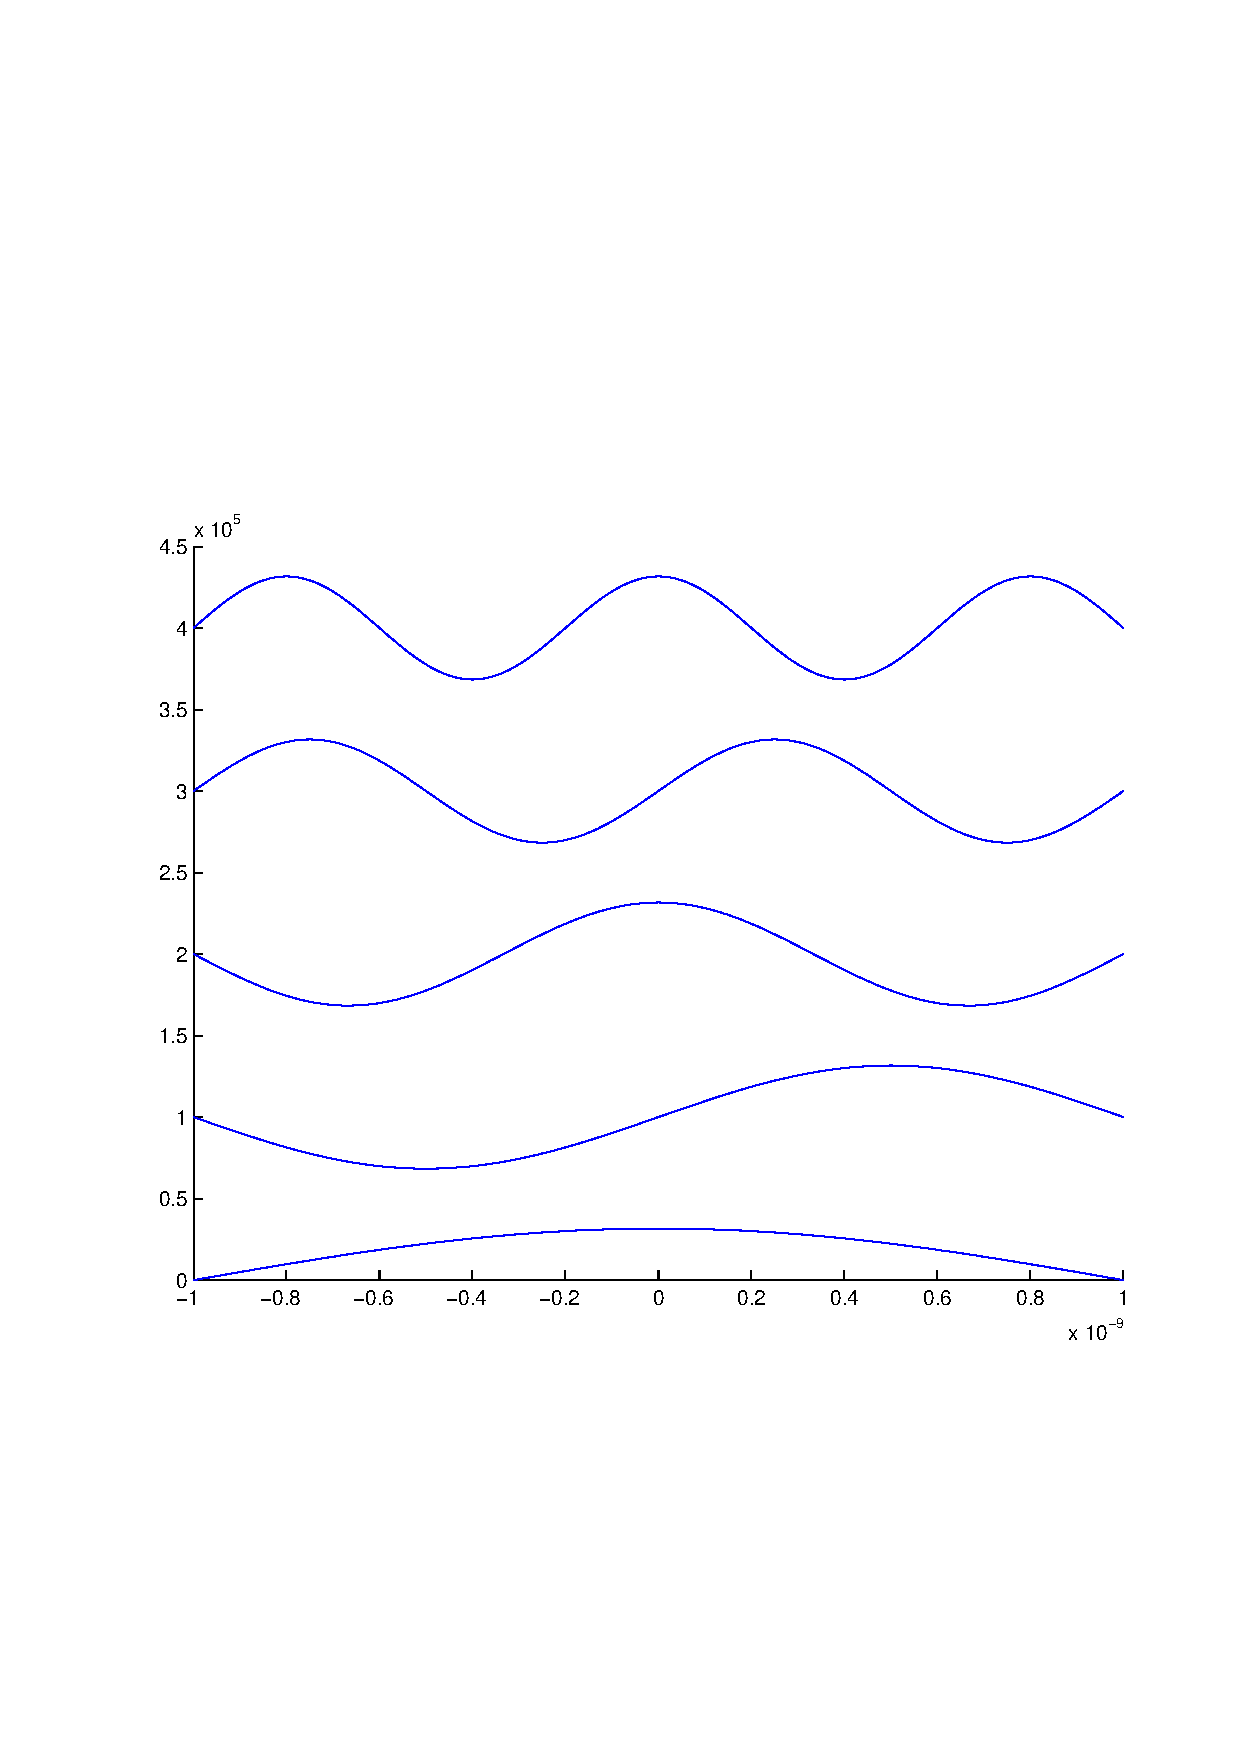
\includegraphics[width=12cm,clip=true,trim=2cm 7cm 1cm 8cm]{efeld/Psi_ungestoert.pdf}
 \caption{$\psi_k^{(0)}$ - Die ersten f\"unf ungest\"orten Energieniveaus von $H_0$ }
 \label{abb:efeld_psi_ungestoert}
\end{figure}

Bei unserer Anwendung bauen wir auf dem Potentialkasten (Kapitel \ref{subsection:potentialkasten}, Seite \pageref{subsection:potentialkasten}) auf.
Dabei geht es um ein Elektron welches zwischen zwei Barrieren mit unendlich hohem Potential gefangen ist.
Zwischen den Barrieren kann sich das Teilchen mit den Wellenfunktionen
\begin{align}
\psi_k(x)
&=
\begin{cases}
\displaystyle
\frac{1}{\sqrt{l}}\cos\frac{k \pi x}{2l}&\qquad \text{$k$ ungerade}\\
\\
\displaystyle
\frac{1}{\sqrt{l}}\sin\frac{k \pi x}{2l}&\qquad \text{$k$ gerade}.
\end{cases}
\end{align}
bewegen.
Die Gleichung wird bei (\ref{skript:potentialkasten-psi-normiert}) Seite \pageref{skript:potentialkasten-psi-normiert} erkl"art.
Ausserhalb des Potentialkastens kommt das Elektron nicht vor.
Es hat die Energie
\[
E_k = \frac{h^2n^2}{32ml^2}
\]
welche bei (\ref{skript:potentialkasten-e})
Seite \pageref{skript:potentialkasten-e} erkl"art wird.

Wir legen jetzt eine Spannung "uber dem Potentialkasten an
und erweitern so das System mit einer St"orung.

Weil das Elektron eine negative Ladung besitzt ver"andert sich seine Wellenfunktion.
Als Grundlagen verwenden wir die Hamiltonfunktion und das Potential des Teilchens im Potentialkasten
\begin{equation}
\begin{aligned}
H_0&=\frac1{2m}p^2+V_0(x)
\\
V_0(x)&=
  \begin{cases}
    0       & \qquad |x|<l\\
    \infty  & \qquad\text{sonst}
  \end{cases}
\end{aligned}
\end{equation}
und erweitern sie mit der St"orung $H_1$ (Abbildung \ref{abb:efeld_H_1}), welche wir als lineares 
Potential definieren:
\begin{equation}
	\label{eq:efeld_H_1}
  H_1 = V_1(x) = a x + b
\end{equation}

\begin{figure}
  \centering
\begin{tikzpicture}
  \shade[top color=gray!20,bottom color=gray!20] 
      (0,0) (1,1) |- (0,0);
  \shade[top color=gray!20,bottom color=gray!20] 
      (-1,-1) |- (0,0) (-1,-1);
  \draw[->] (-1.4,0) -- (1.4,0) node[right] {$x$};
  \draw[->] (0,-1.4) -- (0,1.4) node[above] {$V_1$};
  \draw[scale=0.5,domain=-2:2,smooth,variable=\x,red] plot ({\x},{\x});
\end{tikzpicture}
 \caption{St\"orung $H_1$}
 \label{abb:efeld_H_1}
\end{figure}

Da das Potential die Stammfunktion des elektrischen Feldes ist, entspricht der Parameter $b$ der Integrationskonstante.
F\"ur das Potential sind nur Unterschiede relevant, w\"ahrend das Niveau, solange es in der ganzen Anwendung ver\"andert wird,
beliebig gew\"ahlt werden kann. Somit k\"onnen wir mit $b=0$ die Formel nochmals vereinfachen.

Die Feldst\"arke $a$ h\"angt von der Breite des Potentialkastens $2 l$ und der angelegten Spannung $U$ ab.
\[
  a = \frac{ U }{2 l}
\]
Diese Funktion dr\"uckt mit dem Parameter $U$ das eingeschaltete elektrische Feld \"uber dem Potentialkasten aus
und erf\"ullt damit die selbe Funktion wie das $\varepsilon$.
Wollen wir nun die Formeln mit $a=1$ vereinfachen, m\"ussen wir alle relevanten Terme  in $\varepsilon$ unterbringen

\begin{equation}
\begin{aligned}
  \varepsilon H_1(x) &= \varepsilon a e_{-} x +b  \\
                     &= \varepsilon \frac{ U }{2 l} e_{-} x + 0  \\ 
  \Longrightarrow \qquad \varepsilon &= \frac{ U }{2 l} e_{-} \, \text{ und } \, a = 1
\end{aligned}
\end{equation}
Wenn wir jetzt die St"orung einsetzen, bekommen wir die neue Hamilton-Funktion
\[
  H = H_0 + H_1 
    = \frac1{2m}p^2+V_0(x) + \varepsilon x
\]
aus welcher wir den Hamilton-Operator
\[
  \hat{H} = -\frac{\hbar^2}{2m} \frac{\partial^2}{\partial x^2} + V_0(x) + \varepsilon x
\]
berechnen k"onnen.

\subsection{Vorgehensweise}
Wir berechnen in unserem Beispiel die erste N"aherung.
Im Kapitel \ref{skript:stoerungsloesung1ordnung} St\"orungstheorie wird dies 
theoretisch ausgef\"uhrt.

Entscheidend ist hier ob die Zust"ande entartet sind oder nicht.
Entartung bedeutet, dass zwei Zust"ande die selbe Energie besitzen, 
wodurch bei der Berechnung der Nenner zu Null wird.
Wir sehen an der Gleichung
\[
  E_n^{(0)} = \frac{h^2n^2}{32ml^2}
\]
dass die Energie mit zunehmendem $n$ immer steigt. 
Zudem haben wir f\"ur jedes $n$ nur genau einen Zustand und dadurch keine Entartung. 
Deshalb k\"onnen wir die Gleichungen
\begin{equation}
\begin{aligned}
\label{eq:efeld_E_Skalarprodukt}
E_k^{(1)} &=
\langle \psi_k^{(0)}|\, H_1 \,|\psi_k^{(0)}\rangle
&&\Longrightarrow
& E_k(\varepsilon)&=E_k^{(0)} + \varepsilon E_k^{(1)}
\\
\langle\psi_l^{(0)}|\psi_k^{(1)}\rangle
&=
\frac{\langle \psi_l^{(0)}|\, H_1 \,|\psi_k^{(0)}\rangle}{E_k^{(0)}-E_l^{(0)}}
&&\Longrightarrow
& |\psi_k(\varepsilon)\rangle &=
(1+i\varepsilon \gamma)
\,|\psi_k^{(0)}\rangle
+
\varepsilon
\sum_{k\ne l}
\frac{\langle \psi_l^{(0)}|\, H_1 \,|\psi_k^{(0)}\rangle}{E_k^{(0)}-E_l^{(0)}}
\,
|\psi_l^{(0)}\rangle
\end{aligned}
\end{equation}
aus dem Kapitel \ref{section:nichtentartetezustaende}, Seite \pageref{section:nichtentartetezustaende} verwenden.

Mit $\gamma$ kann die Wellenfunktion normiert werden.
Das ist n"otig, wenn die St"orung Energie hinzuf"ugt
und so die Wahrscheinlichkeitsverteilung ($P \ne 1$) nicht mehr stimmen w\"urde.
Weil wir aber in der ersten N\"aherung keine 
Energiever\"anderung durch die St\"orung bekommen, m\"ussen wir
\begin{equation}
  \label{eq:efeld_gamma}
  \gamma = 0
\end{equation}
setzen.




\subsection{Symmetrie"uberlegung}
\index{Potentialkasten!Symmetrie}
\index{Symmetrien!Energie}
Mit der Gleichung \ref{eq:efeld_E_Skalarprodukt} k"onnen wir direkt die Energie der St"orung berechnen.
\begin{equation}
\begin{aligned}
  E_{k}^{(1)} 
 &= \langle \psi_k^{(0)}|\, H_1 \,|\psi_k^{(0)}\rangle 
  = \langle \psi_k^{(0)}|\, x \;|\psi_k^{(0)}\rangle                   \\
 &= \int_{-L}^{L} \overline{\psi_k^{(0)}} x \; \psi_k^{(0)} dx
  = \int_{-L}^{L} \psi_n(x) \, x \, \psi_n(x) dx
\end{aligned}
\end{equation}

Mit Symmetrie\"uberlegungen wollen wir nun das Resultat vorhersagen um allf\"allige Fehler erkennen zu k\"onnen.
Bei der Betrachtung von Symmetrien an Funktionen erkennen wir den Zustand an den Exponenten.
Betrachten wir einige Beispiele 
\footnote{Formeln aus den Gleichungen \ref{skript:potentialkasten-psi-normiert} und \ref{eq:efeld_H_1}}
\begin{equation}
\begin{aligned}
x^1 &\Rightarrow \text{ungerade Funktion}
\\
x^2 &\Rightarrow \text{gerade Funktion}
\\
\frac{1}{\sqrt{l}}\cos\left( \frac{n \pi x}{2l} \right)  &\Rightarrow \text{gerade Funktion}
\\
\frac{1}{\sqrt{l}}\sin\left( \frac{n \pi x}{2l} \right)  &\Rightarrow \text{ungerade Funktion}
\end{aligned}
\end{equation}
Betrachten wir unsere Funktionen in Abbildung \ref{abb:efeld_gerade_ungerade} so stellen wir fest, 
dass gerade Funktionen nur Terme mit geraden Exponenten besitzen und achsensymmetrisch sind.
Ungerade sind punktsymmetrisch.

\begin{figure}
  \centering
\begin{tikzpicture}
  \draw[->] (-3.2,0) -- (3.2,0) node[right] {$x$};
  \draw[->] (0,-1.7) -- (0,3.5) node[above] {$y$};
  \draw[scale=1,domain=-1.9:1.9,smooth,variable=\x,blue] plot ({\x},{\x*\x});
  \draw[scale=1,domain=-3:3,smooth,variable=\x,blue]  plot ({\x},{cos(90*\x)});
  \draw[scale=1,domain=-1.8:2.2,smooth,variable=\x,red] plot ({\x},{\x});
  \draw[scale=1,domain=-3:3,smooth,variable=\x,red]  plot ({\x},{sin(90*\x)});
\end{tikzpicture}
 \caption{Gerade Funktionen $x^2$ und $\cos(x)$ in blau, ungerade Funktionen $x$ und $\sin(x)$ in rot}
 \label{abb:efeld_gerade_ungerade}
\end{figure}

Dass die Sinus-Funktion ungerade ist, spielt in diesem Fall keine Rolle, da wir mit 
\[
  \overline{\sin(x)} \sin(x) = |\sin(x)|^2
\]
wieder eine gerade Funktion erhalten.

Allerdings bekommen wir immer eine ungerade Funktion, wenn wir eine gerade Funktion mit einer ungeraden Funktion multiplizieren:
\[ 
  x \cdot \overline{\psi_k^{(0)}(x)} \psi_k^{(0)}(x) = x \cdot |\psi_k^{(0)}(x)|^2
\]

Wir k"onnen das Skalarprodukt auch als ein Integral verstehen.
Da ungerade Funktionen punktsymmetrisch sind, muss das Integral $0$ sein:
\[
  E_k^{(1)} = \int_{-L}^{+L} x |\psi_k^{(0)}|^2 dx = 0 .
\]

Wir k"onnen die Energie trotzdem in
$E_k(\varepsilon)=E_k^{(0)} + \varepsilon E_k^{(1)}$ einsetzen
und bekommen so die st"orungsabh"angige Energie.






\subsubsection{Wahrscheinlichkeitsverteilung}
\index{Symmetrien!Wahrscheinlichkeitsverteilung}

Um $\psi_k(\varepsilon)$ zu berechnen wird es etwas schwieriger,
weil sich in der Quantenmechanik die Energiezust"ande $k$ gegenseitig beeinflussen.
Wir setzen daher eine St"orung $\psi_k^{(1)}$ aus mehreren $\psi_k^{(0)}$ zusammen.
Mit der zweiten Formel k"onnen wir den Anteil der jeweiligen $\psi_k^{(1)}$ berechnen.
Wir berechnen 
\[
\psi_k^{(1)} =
\sum_{k\ne l}
\langle\psi_l^{(0)}|\psi_k^{(1)}\rangle |\psi_l^{(0)}\rangle + \gamma|\psi_k^{(0)}\rangle
=
\sum_{k\ne l}
\frac{\langle \psi_l^{(0)}|\, H_1 \,|\psi_k^{(0)}\rangle}{E_k^{(0)}-E_l^{(0)}} |\psi_l^{(0)}\rangle
\]
wobei wir den Term um $\gamma$ durch die Definition (\ref{eq:efeld_gamma}) weglassen k\"onnen.

Wir "uberlegen uns auch hier die Symmetrie.
$\psi_k^{(0)}$ und $\psi_l^{(0)}$ k"onnen sowohl gerade als auch ungerade sein,
$H_1$ ist hingegen immer ungerade.
Uns interessieren die Skalarprodukte die gerade sind, denn nur die ergeben einen Beitrag.
Das ist der Fall wenn $H_1$ und $\psi_k^{(0)} \psi_l^{(0)}$ ungerade sind.
$\langle \psi_l^{(0)}|\, H_1 \,|\psi_k^{(0)}\rangle$ ergibt nur einen Beitrag wenn die Bedingung
\begin{equation}
  \label{eq:efeld_summebedingung}
  k-l \equiv 1 \mod 2
\end{equation}
welche den Rechenaufwand halbiert und $k \ne l$ bereits enh\"alt.



\subsection{Matlab Umgebung}

Matlab\footnote{MATrix LABoratory} ist ein Programm welches sich gut zum Plotten von Funktionen
und zum Berechnen von Matrizen eignet.
Besonders das Berechnen von Matrizen und Vektoren wird durch die Syntax erleichtert.

Eine Auswahl der verwendeten Befehle zum besseren Verst"andnis:

\begin{center}
	\index{Matlab!Syntax}
	\begin{tabular}{lp{9cm}}
		\verb|vektor = n : m| & ein Vektor mit Elementen von $n$ bis $m$ mit Schrittweite $1$. \\
		\verb|vektor = n : delta : m| & ein Vektor mit Elementen von $n$ bis $m$, welche voneinander den Abstand $delta$ haben. \\
		\verb|vector(:)| & alle Werte aus dem Vektor $vektor$ werden ausgelesen. \\
		\verb|matrix * matrix| & Matrix-Multiplikation. \\
		\verb|vector .* vector| & multipliziere die Elemente der Vektoren. \\
		\verb|dot(a, b)| & bildet das Skalarprodukt von $a$ und $b$.
	\end{tabular}
\end{center}




\subsection{Berechnung des Modells mit Matlab}

Wir wollen jetzt die Wellen $\psi_k(\varepsilon)$ und die Energie auch tats"achlich berechnen.
Dazu verwenden wir das Programm Matlab.

Wie beginnen damit, dass wir Konstanten und das ungest"orte System bestimmen.
Wir definieren f"ur unseren Potentialkasten eine Breite von $10^{-9}$ (1nm links und rechts)
\begin{lstlisting}[style=Matlab]
L = 10^-9;                         # Entfernung der Grenzen der Simulation
n = 1000;                          # Anzahl aufsummierter Zustaende
xSteps = 500;                      # Anzahl Abtastwerte in x-Richtung
x = -L : 2*L/xSteps : +L;          # Vektor von -L bis +L mit xSteps Schritten
\end{lstlisting}
und bekommen so den Vektor $x$.

Um die ungest"orten Zust"ande $\psi_k^{(0)}$ zu bekommen, tasten wir die Sinus- und Kosinus-Funktion 
aus der Gleichung (\ref{skript:potentialkasten-psi-normiert}) Seite \pageref{skript:potentialkasten-psi-normiert} diskret ab.

Gleichzeitig bestimmen wir die Energien $E_k^{(0)}$.
\begin{lstlisting}[style=Matlab]
m = 9.10938291*10^-31;             # Elektronenmasse
h = 6062606957*10^-34;             # Planck-Konstante

for k = 1 : n
    E0(k) = h^2*k^2 / (32*m*L^2);
    
    if mod(k, 2) == 0              # Gerade k
        y = sin(k*pi*x/(2*L));
    else                           # Ungerade k
        y = cos(k*pi*x/(2*L));
    end
    Psi(k, x) = 1/sqrt(2*L) .* y;
end
\end{lstlisting}
und bekommen so einen Vektor mit den $n$ Werten f"ur $E_k^{(0)}$
sowie eine Matrix $\texttt{xSteps} \times \texttt{n}$ (konkret $500 \times 1000$) f"ur $\psi_k^{(0)}$.

\subsection{Berechnung von $E_k^{(1)}$}

Nun, da wir die Grundlagen berechnet haben, k"onnen wir $\psi_k(\varepsilon)$ und 
$E_k(\varepsilon)$ berechnen. Die Energie darf sich in der 1. N\"aherung nicht ver\"andern.
Dieses Resultat zeigt uns die Robustheit der Berechnungen auf.

Implementiert wurde der Test wie folgt:
\begin{lstlisting}[style=Matlab]
H1 = x;
for k = 1 : 5
  E1(k) = dot(Psi(k, :), H1.*Psi(k, :));
  plot(epsilon, E0(k) + epsilon*E1_k(k))
end
\end{lstlisting}
Das Resultat ist in diesem Fall mit Vorsicht zu geniessen.
Weil wir mit diskreten Werten arbeiten, entsteht beim Skalarprodukt ein Fehler von ca. $8 \cdot 10^{-15}$,
welches mit einem korrektem Wert verwechselt werden kann.
Den Plot sehen wir in der Abbildung \ref{abb:efeld_E_gestoert}.
Wir schliessen daraus, dass die Berechnung stabil ist und die Werte genau genug sind.





\subsection{Berechnung von $\psi_k^{(1)}$}

Die Implementierung von $\psi_k^{(1)}$ gestaltet sich durch die Summe etwas schwieriger.
Normalerweise k"onnte man mit \verb|sum(vektor)| alle Elemente zusammenz"ahlen lassen.
Wir ber\"ucksichtigen aber Bedingung aus (\ref{eq:efeld_summebedingung}) um den Rechenaufwand zu halbieren
und um Division durch $0$ zu vermeiden.

Um zum Beispiel den f"unften Zustand zu bestimmen, summieren wir alle Zust\"ande vom 
ersten bis $n$-ten ausser den ungeraden.
\begin{equation}
  \psi_5^{(1)} = \langle\psi_l^{(0)}|\psi_5^{(1)}\rangle|\psi_l^{(0)}\rangle = 
  \sum_{l=1 \, \text{wenn} \, 5-l \equiv 1 \mod 2}^{n}
    \frac{\langle \psi_l^{(0)}|\, H_1 \,|\psi_k^{(0)}\rangle}{E_k^{(0)}-E_l^{(0)}}
        \,
    |\psi_l^{(0)}\rangle
\end{equation}

In Matlab wird das wie folgt implementiert:
\begin{lstlisting}[style=Matlab]
H1 = x * -1;               # Die Stoerung des elektrische Feldes mit dem
                           #   Faktor -1, da das Elektron negativ geladen ist
n = 1000;                  # Anzahl aufsummierter Zustaende
k = 5;                     # Der Zustand den wir plotten
summe = 0;                 # Initialisierung des SummenVektors

for l = 1 : n
  if mod((l + k), 2) == 1  # Vergleich l ungleich k und Differenz ungerade
    Psi_lk = dot(Psi(l, :), H1.*Psi(k, :)) / (E0(k)-E0(l)) .* Psi(l, :);
    summe = summe + Psi_lk;
  end
end
\end{lstlisting}
Die Variable \verb|summe| ist nun ein Vektor mit den diskreten Abtastwerten von $\psi_k^{(1)}$.

Mit der Abfrage \verb|mod((l + k), 2) == 1| werden die Summanden 
entsprechend der Symmetrie"uberlegung gefiltert.
Gleichzeitig wird der Term f"ur $l=k$ entfernt ($0 mod 2 \ne 1$).
Der Anteil der Summanden am Gesammtzustand nimmt dabei mit jedem Schritt weiter ab.
Der Grund ist die stetige Zunahme des Terms $E^{(0)}_k-E^{(0)}_l$ unter dem Bruchstrich.
In diesem Fall addieren wir beim 90-sten Schritt ($l=90$) nur $1\%$ der St"orung dazu.
Beim 280-sten Schritt ($l=280$) betr"agt der Anteil nur noch $0.1\%$.

Wir k"onnen jetzt die St"orung in 
\begin{equation}
|\psi_k(\varepsilon)\rangle
=
(1+i\varepsilon \gamma)
\,|\psi_k^{(0)}\rangle
+
\varepsilon|\psi_k^{(1)}\rangle
\end{equation}
einsetzen und bekommen so die neue Wellenfunktion dargestellt in Abbildung \ref{abb:efeld_psi_gestoert}.




\subsection{Auswertung Psi}

In der Grafik \ref{abb:efeld_psi_gestoert} sehen wir die Unterschiede zwischen den ungest"orten 
$\psi_k$ (schwarz) und der ersten N"aherung (rot).
Der \"Ubersicht halber haben wir die Amplituden von $\psi_k$ in einzelnen Graphen dargestellt.

Die einzelnen Grafiken zeigen sehr anschaulich wie der Unterschied zwischen dem ungest\"orten und dem gest\"orten $\psi$
immer kleiner wird.

\begin{figure}
 \centering
 \includegraphics[width=12cm,clip=true,trim=2cm 6.6cm 1cm 8cm]{efeld/Psi_SubPlots_gestoert.pdf}
 \caption{einige Energieniveaus von $\psi$, ungest\"ort in blau und gest"ort in rot.}
 \label{abb:efeld_psi_gestoert}
\end{figure}

Die Funktion 
\[
  \psi \cdot \overline{\psi} = |\psi|^2
\]
entspricht der Wahrscheinlichkeitsdichte, 
dass sich das Elektron an dieser Stelle befindet.
Auf der Horizontalen sehen wir die $x$-Position vom Teilchen im eindimensionalen Potentialkasten.

Intuitiv nimmt man an, dass die Wellenfunktion durch die St\"orung $H_1$ in der Abbildung 
\ref{abb:efeld_H_1} nach links gedr"uckt werden wird, da das elektrische Feld 
im ersten Quadranten ein positives Potential bildet und deshalb das Elektron herunter rollen m\"ochte.
\[
  H_1(x) = x
\]

Allerdings wird durch die positive Spannung das Elektron angezogen und die
Wahrscheinlichkeit es weiter rechts anzutreffen steigt.

Durch das elektrische Feld haben wir entlang der $x$-Achse verschieden Energie-Potentiale.
Das Elektron hat allerdings immer die selbe Energie,
die Energie muss sich also irgendwie ausgleichen.
Wir k"onnen diesen Vorgang mit der Schr"odingergleichung einfach verstehen:
\[
-\frac{\hbar^2}{2m}\Delta\Psi(x) + V(x)\Psi(x)
=
E \Psi(x)
\]
Weil $E \Psi(x)$ konstant ist, sinkt bei einem h"oherem Potential $-\frac{\hbar^2}{2m}\Delta\Psi(x)$.
Das bedeutet bei einem Elektron eine Abnahme der kinetischen Energie bzw. der Frequenz.
Der Vorgang ist also "ahnlich einem mechanischem Pendel, 
welches mal kinetische Energie hat, mal potentielle.



\subsubsection{100-stes Energieniveau}
% FIXME Beschreibung zum 100-sten korrekt? Das Wort Welle kommt zu oft vor!
Betrachten wir nun das 100-ste Energieniveau etwas genauer.
In der Abbildung \ref{abb:efeld_psi_100_gestoert} sehen wir wie die St\"orung 
die Wellenl\"ange der Wellenfunktion $\psi$ ver\"andert.
Die gelben Balken geben an, wie stark die Periodendauer zwischen zwei Nulldurchg"angen
von der ungest"orten Funktion abweicht.
Wir k"onnen an den Balken gut die Form der St"orung $H_1$ wiedererkennen.

Die Kr"ummung in der Kurve entsteht durch Erh"ohung der Amplitude um den Nullpunkt.
Diese entsteht durch die Stauchung der Wellenfunktion und verursacht das wir mehr Energie
bei gleicher Wellenl\"ange haben.

Summiert man die Fl\"achen auf, so ergeben sie insgesamt wieder $0$, da die Energie sich nicht ver\"andert hat.


\begin{figure}
 \centering
 \includegraphics[width=12cm,clip=true,trim=2cm 7cm 1cm 8cm]{efeld/Psi_100_gestoert.pdf}
 \caption{100-stes Energieniveau von $\psi$ ungest\"ort in blau und gest\"ort in rot, 
          mit der Visualisierung der Verschiebung der Periodendauer in gelb.}
 \label{abb:efeld_psi_100_gestoert}
\end{figure}




\subsection{Auswertung E}

Mit den Symmetrie\"uberlegungen haben wir vorausgesagt, dass sich der Energiezustand nicht \"andert.
Um dies m\"oglichst einfach zu \"uberpr\"ufen, w\"ahlen wir ein grosses $\varepsilon$ und sehen uns das Resultat in der 
Abbildung \ref{abb:efeld_E_gestoert} an.

\begin{figure}
 \centering
 \includegraphics[width=12cm,clip=true,trim=2cm 7cm 1cm 8cm]{efeld/Energie_gestoert.pdf}
 \caption{$E_k^{(1)}$ gest\"ort, horizontale Achse ist $\varepsilon$, vertikale Achse ist die gesamte Energie des Systems}
 \label{abb:efeld_E_gestoert}
\end{figure}

Mit einem gr\"osseren $\varepsilon$ wird der Anteil des nummerischen Fehlers gr\"osser.
Verh\"alt sich das Modell bei einem starken $\varepsilon$ gut, so k\"onnen wir mit diesem sehr einfachen Test
auf die Robustheit der Berechnung von $E_k^{(1)}$ testen.



\section{Vergleich zu Vorhersagen von Louis de Broglie}
% TODO Text

"With every particle of matter with mass m and velocity v a real wave must be 'associated'"
\begin{equation}
  \label{efeld:eq_deBroglie}
  \lambda = \frac{h}{p} = \frac {h}{{m}{v}} \sqrt{1 - \frac{v^2}{c^2}}
\end{equation}


Wir vereinfachen die Gleichung \ref{efeld:eq_deBroglie} mit
\[
  v \approx 0
\]
da sich unser Elektron gegen\"uber der Lichtgeschwindigkeit $c$ fast nicht bewegt:
\begin{equation}
  \lambda = \frac{h}{p} \approx \frac{h}{m v}
\end{equation}




\printbibliography[heading=subbibliography]
\end{refsection}

\chapter{Geladenes Teilchen im elektrischen Feld\label{chapter:efeld}}
\lhead{Teilchen im elektrischen Feld}
\begin{refsection}
\chapterauthor{Michael Cerny und Stefan Schindler}

\index{Potentialkasten!Anwendung}


In diesem Kapitel erweitern wir das Beispiel des Potentialkastens 
(Kapitel \ref{subsection:potentialkasten}, Seite \pageref{subsection:potentialkasten})
um eine St\"orung so, dass wir ein Elektron mit einem elektrischen Feld st\"oren.
Im speziellen betrachten wir Symmetrien in den Wellenfunktionen.
Mit diese Betrachtungen halbieren wir den Aufwand der nummerischen Berechnung.

Die nummerische Berechnung der 1. N\"aherung wird in diesem Kapitel mit Matlab realisiert und dokumentiert. 
F\"ur die Simulation wurden empirisch realistische Werte gew\"ahlt.
Der gesammte Code ist auf der beiligenden CD enthalten.

Zum Schluss warten wir noch mit einem kleinen Vergleich zu den Aussagen von de Broglie \cite{efeld:de_Broglie} auf.
Wir w\"unschen viel Vergn\"ugen beim Lesen.



\section{Grundlagen St"orungstheorie}
Grunds"atzlich k"onnen wir mit der St\"orungstheorie ein einfaches Modell 
(Abbildung \ref{abb:efeld_psi_ungestoert} der ersten 5 Energieniveaus) 
mit einer St\"orung erg"anzen, statt von Anfang an mit einem komplexen Modell zu rechnen.

F"ur die erste N"aherung gilt:
\[
  f(x, \varepsilon) = f_0(x) + \varepsilon f_1(x)
\]
Dabei ist $f_0(x)$ die ungest"orte Funktion und $\varepsilon f_1(x)$ die St"orung.
$\varepsilon$ ist eine Variable, mit der wir den St"orungsterm $f_1(x)$ steuern.
Dabei sollte $\varepsilon$ nicht zu gross gew"ahlt werden,
da die N"aherung sonst ungenau wird.
Setzen wir hingegen $\varepsilon = 0$, k\"onnen wir die St"orung dynamisch abschalten.




In der Quantenmechanik k"onnen wir die St"orungstheorie anwenden,
indem wir den Hamilton-Operator der urspr"unglichen Funktion $H_0$
um $\varepsilon H_1$ erg"anzen:
\[
  H = H_0 + \varepsilon H_1.
\]

Indem wir die Energie und die Wellenfunktion der St"orung berechnen, k"onnen wir das gest"orte System ganz einfach beschreiben:
\begin{equation}
\begin{aligned}
E_k(\varepsilon)&=E_k^{(0)} + \varepsilon E_k^{(1)}
\\
\psi_k(\varepsilon)&=\psi_k^{(0)} + \varepsilon \psi_k^{(1)}
\end{aligned}
\end{equation}

Ein grosser Vorteil dabei ist,
dass wir die St"orungsterme $E_k^{(1)}$ und $\psi_k^{(1)}$
direkt aus dem ungest"ortem System berechnen k"onnen,
ohne nochmals die Schr"odingergleichung l"osen zu m"ussen.
Wir m"ussen also f"ur die erste N"aherung nur $E_k^{(0)}$,
$\psi_k^{(0)}$ und $\varepsilon$ kennen.




\section{Potentialkasten mit elektrischem Feld}

\subsection{Ausgangslage}

\begin{figure}
 \centering
 \includegraphics[width=12cm,clip=true,trim=2cm 7cm 1cm 8cm]{efeld/Psi_ungestoert.pdf}
 \caption{$\psi_k^{(0)}$ - Die ersten f\"unf ungest\"orten Energieniveaus von $H_0$ }
 \label{abb:efeld_psi_ungestoert}
\end{figure}

Bei unserer Anwendung bauen wir auf dem Potentialkasten (Kapitel \ref{subsection:potentialkasten}, Seite \pageref{subsection:potentialkasten}) auf.
Dabei geht es um ein Elektron welches zwischen zwei Barrieren mit unendlich hohem Potential gefangen ist.
Zwischen den Barrieren kann sich das Teilchen mit den Wellenfunktionen
\begin{align}
\psi_k(x)
&=
\begin{cases}
\displaystyle
\frac{1}{\sqrt{l}}\cos\frac{k \pi x}{2l}&\qquad \text{$k$ ungerade}\\
\\
\displaystyle
\frac{1}{\sqrt{l}}\sin\frac{k \pi x}{2l}&\qquad \text{$k$ gerade}.
\end{cases}
\end{align}
bewegen.
Die Gleichung wird bei (\ref{skript:potentialkasten-psi-normiert}) Seite \pageref{skript:potentialkasten-psi-normiert} erkl"art.
Ausserhalb des Potentialkastens kommt das Elektron nicht vor.
Es hat die Energie
\[
E_k = \frac{h^2n^2}{32ml^2}
\]
welche bei (\ref{skript:potentialkasten-e})
Seite \pageref{skript:potentialkasten-e} erkl"art wird.

Wir legen jetzt eine Spannung "uber dem Potentialkasten an
und erweitern so das System mit einer St"orung.

Weil das Elektron eine negative Ladung besitzt ver"andert sich seine Wellenfunktion.
Als Grundlagen verwenden wir die Hamiltonfunktion und das Potential des Teilchens im Potentialkasten
\begin{equation}
\begin{aligned}
H_0&=\frac1{2m}p^2+V_0(x)
\\
V_0(x)&=
  \begin{cases}
    0       & \qquad |x|<l\\
    \infty  & \qquad\text{sonst}
  \end{cases}
\end{aligned}
\end{equation}
und erweitern sie mit der St"orung $H_1$ (Abbildung \ref{abb:efeld_H_1}), welche wir als lineares 
Potential definieren:
\begin{equation}
	\label{eq:efeld_H_1}
  H_1 = V_1(x) = a x + b
\end{equation}

\begin{figure}
  \centering
\begin{tikzpicture}
  \shade[top color=gray!20,bottom color=gray!20] 
      (0,0) (1,1) |- (0,0);
  \shade[top color=gray!20,bottom color=gray!20] 
      (-1,-1) |- (0,0) (-1,-1);
  \draw[->] (-1.4,0) -- (1.4,0) node[right] {$x$};
  \draw[->] (0,-1.4) -- (0,1.4) node[above] {$V_1$};
  \draw[scale=0.5,domain=-2:2,smooth,variable=\x,red] plot ({\x},{\x});
\end{tikzpicture}
 \caption{St\"orung $H_1$}
 \label{abb:efeld_H_1}
\end{figure}

Da das Potential die Stammfunktion des elektrischen Feldes ist, entspricht der Parameter $b$ der Integrationskonstante.
F\"ur das Potential sind nur Unterschiede relevant, w\"ahrend das Niveau, solange es in der ganzen Anwendung ver\"andert wird,
beliebig gew\"ahlt werden kann. Somit k\"onnen wir mit $b=0$ die Formel nochmals vereinfachen.

Die Feldst\"arke $a$ h\"angt von der Breite des Potentialkastens $2 l$ und der angelegten Spannung $U$ ab.
\[
  a = \frac{ U }{2 l}
\]
Diese Funktion dr\"uckt mit dem Parameter $U$ das eingeschaltete elektrische Feld \"uber dem Potentialkasten aus
und erf\"ullt damit die selbe Funktion wie das $\varepsilon$.
Wollen wir nun die Formeln mit $a=1$ vereinfachen, m\"ussen wir alle relevanten Terme  in $\varepsilon$ unterbringen

\begin{equation}
\begin{aligned}
  \varepsilon H_1(x) &= \varepsilon a e_{-} x +b  \\
                     &= \varepsilon \frac{ U }{2 l} e_{-} x + 0  \\ 
  \Longrightarrow \qquad \varepsilon &= \frac{ U }{2 l} e_{-} \, \text{ und } \, a = 1
\end{aligned}
\end{equation}
Wenn wir jetzt die St"orung einsetzen, bekommen wir die neue Hamilton-Funktion
\[
  H = H_0 + H_1 
    = \frac1{2m}p^2+V_0(x) + \varepsilon x
\]
aus welcher wir den Hamilton-Operator
\[
  \hat{H} = -\frac{\hbar^2}{2m} \frac{\partial^2}{\partial x^2} + V_0(x) + \varepsilon x
\]
berechnen k"onnen.

\subsection{Vorgehensweise}
Wir berechnen in unserem Beispiel die erste N"aherung.
Im Kapitel \ref{skript:stoerungsloesung1ordnung} St\"orungstheorie wird dies 
theoretisch ausgef\"uhrt.

Entscheidend ist hier ob die Zust"ande entartet sind oder nicht.
Entartung bedeutet, dass zwei Zust"ande die selbe Energie besitzen, 
wodurch bei der Berechnung der Nenner zu Null wird.
Wir sehen an der Gleichung
\[
  E_n^{(0)} = \frac{h^2n^2}{32ml^2}
\]
dass die Energie mit zunehmendem $n$ immer steigt. 
Zudem haben wir f\"ur jedes $n$ nur genau einen Zustand und dadurch keine Entartung. 
Deshalb k\"onnen wir die Gleichungen
\begin{equation}
\begin{aligned}
\label{eq:efeld_E_Skalarprodukt}
E_k^{(1)} &=
\langle \psi_k^{(0)}|\, H_1 \,|\psi_k^{(0)}\rangle
&&\Longrightarrow
& E_k(\varepsilon)&=E_k^{(0)} + \varepsilon E_k^{(1)}
\\
\langle\psi_l^{(0)}|\psi_k^{(1)}\rangle
&=
\frac{\langle \psi_l^{(0)}|\, H_1 \,|\psi_k^{(0)}\rangle}{E_k^{(0)}-E_l^{(0)}}
&&\Longrightarrow
& |\psi_k(\varepsilon)\rangle &=
(1+i\varepsilon \gamma)
\,|\psi_k^{(0)}\rangle
+
\varepsilon
\sum_{k\ne l}
\frac{\langle \psi_l^{(0)}|\, H_1 \,|\psi_k^{(0)}\rangle}{E_k^{(0)}-E_l^{(0)}}
\,
|\psi_l^{(0)}\rangle
\end{aligned}
\end{equation}
aus dem Kapitel \ref{section:nichtentartetezustaende}, Seite \pageref{section:nichtentartetezustaende} verwenden.

Mit $\gamma$ kann die Wellenfunktion normiert werden.
Das ist n"otig, wenn die St"orung Energie hinzuf"ugt
und so die Wahrscheinlichkeitsverteilung ($P \ne 1$) nicht mehr stimmen w\"urde.
Weil wir aber in der ersten N\"aherung keine 
Energiever\"anderung durch die St\"orung bekommen, m\"ussen wir
\begin{equation}
  \label{eq:efeld_gamma}
  \gamma = 0
\end{equation}
setzen.




\subsection{Symmetrie"uberlegung}
\index{Potentialkasten!Symmetrie}
\index{Symmetrien!Energie}
Mit der Gleichung \ref{eq:efeld_E_Skalarprodukt} k"onnen wir direkt die Energie der St"orung berechnen.
\begin{equation}
\begin{aligned}
  E_{k}^{(1)} 
 &= \langle \psi_k^{(0)}|\, H_1 \,|\psi_k^{(0)}\rangle 
  = \langle \psi_k^{(0)}|\, x \;|\psi_k^{(0)}\rangle                   \\
 &= \int_{-L}^{L} \overline{\psi_k^{(0)}} x \; \psi_k^{(0)} dx
  = \int_{-L}^{L} \psi_n(x) \, x \, \psi_n(x) dx
\end{aligned}
\end{equation}

Mit Symmetrie\"uberlegungen wollen wir nun das Resultat vorhersagen um allf\"allige Fehler erkennen zu k\"onnen.
Bei der Betrachtung von Symmetrien an Funktionen erkennen wir den Zustand an den Exponenten.
Betrachten wir einige Beispiele 
\footnote{Formeln aus den Gleichungen \ref{skript:potentialkasten-psi-normiert} und \ref{eq:efeld_H_1}}
\begin{equation}
\begin{aligned}
x^1 &\Rightarrow \text{ungerade Funktion}
\\
x^2 &\Rightarrow \text{gerade Funktion}
\\
\frac{1}{\sqrt{l}}\cos\left( \frac{n \pi x}{2l} \right)  &\Rightarrow \text{gerade Funktion}
\\
\frac{1}{\sqrt{l}}\sin\left( \frac{n \pi x}{2l} \right)  &\Rightarrow \text{ungerade Funktion}
\end{aligned}
\end{equation}
Betrachten wir unsere Funktionen in Abbildung \ref{abb:efeld_gerade_ungerade} so stellen wir fest, 
dass gerade Funktionen nur Terme mit geraden Exponenten besitzen und achsensymmetrisch sind.
Ungerade sind punktsymmetrisch.

\begin{figure}
  \centering
\begin{tikzpicture}
  \draw[->] (-3.2,0) -- (3.2,0) node[right] {$x$};
  \draw[->] (0,-1.7) -- (0,3.5) node[above] {$y$};
  \draw[scale=1,domain=-1.9:1.9,smooth,variable=\x,blue] plot ({\x},{\x*\x});
  \draw[scale=1,domain=-3:3,smooth,variable=\x,blue]  plot ({\x},{cos(90*\x)});
  \draw[scale=1,domain=-1.8:2.2,smooth,variable=\x,red] plot ({\x},{\x});
  \draw[scale=1,domain=-3:3,smooth,variable=\x,red]  plot ({\x},{sin(90*\x)});
\end{tikzpicture}
 \caption{Gerade Funktionen $x^2$ und $\cos(x)$ in blau, ungerade Funktionen $x$ und $\sin(x)$ in rot}
 \label{abb:efeld_gerade_ungerade}
\end{figure}

Dass die Sinus-Funktion ungerade ist, spielt in diesem Fall keine Rolle, da wir mit 
\[
  \overline{\sin(x)} \sin(x) = |\sin(x)|^2
\]
wieder eine gerade Funktion erhalten.

Allerdings bekommen wir immer eine ungerade Funktion, wenn wir eine gerade Funktion mit einer ungeraden Funktion multiplizieren:
\[ 
  x \cdot \overline{\psi_k^{(0)}(x)} \psi_k^{(0)}(x) = x \cdot |\psi_k^{(0)}(x)|^2
\]

Wir k"onnen das Skalarprodukt auch als ein Integral verstehen.
Da ungerade Funktionen punktsymmetrisch sind, muss das Integral $0$ sein:
\[
  E_k^{(1)} = \int_{-L}^{+L} x |\psi_k^{(0)}|^2 dx = 0 .
\]

Wir k"onnen die Energie trotzdem in
$E_k(\varepsilon)=E_k^{(0)} + \varepsilon E_k^{(1)}$ einsetzen
und bekommen so die st"orungsabh"angige Energie.






\subsubsection{Wahrscheinlichkeitsverteilung}
\index{Symmetrien!Wahrscheinlichkeitsverteilung}

Um $\psi_k(\varepsilon)$ zu berechnen wird es etwas schwieriger,
weil sich in der Quantenmechanik die Energiezust"ande $k$ gegenseitig beeinflussen.
Wir setzen daher eine St"orung $\psi_k^{(1)}$ aus mehreren $\psi_k^{(0)}$ zusammen.
Mit der zweiten Formel k"onnen wir den Anteil der jeweiligen $\psi_k^{(1)}$ berechnen.
Wir berechnen 
\[
\psi_k^{(1)} =
\sum_{k\ne l}
\langle\psi_l^{(0)}|\psi_k^{(1)}\rangle |\psi_l^{(0)}\rangle + \gamma|\psi_k^{(0)}\rangle
=
\sum_{k\ne l}
\frac{\langle \psi_l^{(0)}|\, H_1 \,|\psi_k^{(0)}\rangle}{E_k^{(0)}-E_l^{(0)}} |\psi_l^{(0)}\rangle
\]
wobei wir den Term um $\gamma$ durch die Definition (\ref{eq:efeld_gamma}) weglassen k\"onnen.

Wir "uberlegen uns auch hier die Symmetrie.
$\psi_k^{(0)}$ und $\psi_l^{(0)}$ k"onnen sowohl gerade als auch ungerade sein,
$H_1$ ist hingegen immer ungerade.
Uns interessieren die Skalarprodukte die gerade sind, denn nur die ergeben einen Beitrag.
Das ist der Fall wenn $H_1$ und $\psi_k^{(0)} \psi_l^{(0)}$ ungerade sind.
$\langle \psi_l^{(0)}|\, H_1 \,|\psi_k^{(0)}\rangle$ ergibt nur einen Beitrag wenn die Bedingung
\begin{equation}
  \label{eq:efeld_summebedingung}
  k-l \equiv 1 \mod 2
\end{equation}
welche den Rechenaufwand halbiert und $k \ne l$ bereits enh\"alt.



\subsection{Matlab Umgebung}

Matlab\footnote{MATrix LABoratory} ist ein Programm welches sich gut zum Plotten von Funktionen
und zum Berechnen von Matrizen eignet.
Besonders das Berechnen von Matrizen und Vektoren wird durch die Syntax erleichtert.

Eine Auswahl der verwendeten Befehle zum besseren Verst"andnis:

\begin{center}
	\index{Matlab!Syntax}
	\begin{tabular}{lp{9cm}}
		\verb|vektor = n : m| & ein Vektor mit Elementen von $n$ bis $m$ mit Schrittweite $1$. \\
		\verb|vektor = n : delta : m| & ein Vektor mit Elementen von $n$ bis $m$, welche voneinander den Abstand $delta$ haben. \\
		\verb|vector(:)| & alle Werte aus dem Vektor $vektor$ werden ausgelesen. \\
		\verb|matrix * matrix| & Matrix-Multiplikation. \\
		\verb|vector .* vector| & multipliziere die Elemente der Vektoren. \\
		\verb|dot(a, b)| & bildet das Skalarprodukt von $a$ und $b$.
	\end{tabular}
\end{center}




\subsection{Berechnung des Modells mit Matlab}

Wir wollen jetzt die Wellen $\psi_k(\varepsilon)$ und die Energie auch tats"achlich berechnen.
Dazu verwenden wir das Programm Matlab.

Wie beginnen damit, dass wir Konstanten und das ungest"orte System bestimmen.
Wir definieren f"ur unseren Potentialkasten eine Breite von $10^{-9}$ (1nm links und rechts)
\begin{lstlisting}[style=Matlab]
L = 10^-9;                         # Entfernung der Grenzen der Simulation
n = 1000;                          # Anzahl aufsummierter Zustaende
xSteps = 500;                      # Anzahl Abtastwerte in x-Richtung
x = -L : 2*L/xSteps : +L;          # Vektor von -L bis +L mit xSteps Schritten
\end{lstlisting}
und bekommen so den Vektor $x$.

Um die ungest"orten Zust"ande $\psi_k^{(0)}$ zu bekommen, tasten wir die Sinus- und Kosinus-Funktion 
aus der Gleichung (\ref{skript:potentialkasten-psi-normiert}) Seite \pageref{skript:potentialkasten-psi-normiert} diskret ab.

Gleichzeitig bestimmen wir die Energien $E_k^{(0)}$.
\begin{lstlisting}[style=Matlab]
m = 9.10938291*10^-31;             # Elektronenmasse
h = 6062606957*10^-34;             # Planck-Konstante

for k = 1 : n
    E0(k) = h^2*k^2 / (32*m*L^2);
    
    if mod(k, 2) == 0              # Gerade k
        y = sin(k*pi*x/(2*L));
    else                           # Ungerade k
        y = cos(k*pi*x/(2*L));
    end
    Psi(k, x) = 1/sqrt(2*L) .* y;
end
\end{lstlisting}
und bekommen so einen Vektor mit den $n$ Werten f"ur $E_k^{(0)}$
sowie eine Matrix $\texttt{xSteps} \times \texttt{n}$ (konkret $500 \times 1000$) f"ur $\psi_k^{(0)}$.

\subsection{Berechnung von $E_k^{(1)}$}

Nun, da wir die Grundlagen berechnet haben, k"onnen wir $\psi_k(\varepsilon)$ und 
$E_k(\varepsilon)$ berechnen. Die Energie darf sich in der 1. N\"aherung nicht ver\"andern.
Dieses Resultat zeigt uns die Robustheit der Berechnungen auf.

Implementiert wurde der Test wie folgt:
\begin{lstlisting}[style=Matlab]
H1 = x;
for k = 1 : 5
  E1(k) = dot(Psi(k, :), H1.*Psi(k, :));
  plot(epsilon, E0(k) + epsilon*E1_k(k))
end
\end{lstlisting}
Das Resultat ist in diesem Fall mit Vorsicht zu geniessen.
Weil wir mit diskreten Werten arbeiten, entsteht beim Skalarprodukt ein Fehler von ca. $8 \cdot 10^{-15}$,
welches mit einem korrektem Wert verwechselt werden kann.
Den Plot sehen wir in der Abbildung \ref{abb:efeld_E_gestoert}.
Wir schliessen daraus, dass die Berechnung stabil ist und die Werte genau genug sind.





\subsection{Berechnung von $\psi_k^{(1)}$}

Die Implementierung von $\psi_k^{(1)}$ gestaltet sich durch die Summe etwas schwieriger.
Normalerweise k"onnte man mit \verb|sum(vektor)| alle Elemente zusammenz"ahlen lassen.
Wir ber\"ucksichtigen aber Bedingung aus (\ref{eq:efeld_summebedingung}) um den Rechenaufwand zu halbieren
und um Division durch $0$ zu vermeiden.

Um zum Beispiel den f"unften Zustand zu bestimmen, summieren wir alle Zust\"ande vom 
ersten bis $n$-ten ausser den ungeraden.
\begin{equation}
  \psi_5^{(1)} = \langle\psi_l^{(0)}|\psi_5^{(1)}\rangle|\psi_l^{(0)}\rangle = 
  \sum_{l=1 \, \text{wenn} \, 5-l \equiv 1 \mod 2}^{n}
    \frac{\langle \psi_l^{(0)}|\, H_1 \,|\psi_k^{(0)}\rangle}{E_k^{(0)}-E_l^{(0)}}
        \,
    |\psi_l^{(0)}\rangle
\end{equation}

In Matlab wird das wie folgt implementiert:
\begin{lstlisting}[style=Matlab]
H1 = x * -1;               # Die Stoerung des elektrische Feldes mit dem
                           #   Faktor -1, da das Elektron negativ geladen ist
n = 1000;                  # Anzahl aufsummierter Zustaende
k = 5;                     # Der Zustand den wir plotten
summe = 0;                 # Initialisierung des SummenVektors

for l = 1 : n
  if mod((l + k), 2) == 1  # Vergleich l ungleich k und Differenz ungerade
    Psi_lk = dot(Psi(l, :), H1.*Psi(k, :)) / (E0(k)-E0(l)) .* Psi(l, :);
    summe = summe + Psi_lk;
  end
end
\end{lstlisting}
Die Variable \verb|summe| ist nun ein Vektor mit den diskreten Abtastwerten von $\psi_k^{(1)}$.

Mit der Abfrage \verb|mod((l + k), 2) == 1| werden die Summanden 
entsprechend der Symmetrie"uberlegung gefiltert.
Gleichzeitig wird der Term f"ur $l=k$ entfernt ($0 mod 2 \ne 1$).
Der Anteil der Summanden am Gesammtzustand nimmt dabei mit jedem Schritt weiter ab.
Der Grund ist die stetige Zunahme des Terms $E^{(0)}_k-E^{(0)}_l$ unter dem Bruchstrich.
In diesem Fall addieren wir beim 90-sten Schritt ($l=90$) nur $1\%$ der St"orung dazu.
Beim 280-sten Schritt ($l=280$) betr"agt der Anteil nur noch $0.1\%$.

Wir k"onnen jetzt die St"orung in 
\begin{equation}
|\psi_k(\varepsilon)\rangle
=
(1+i\varepsilon \gamma)
\,|\psi_k^{(0)}\rangle
+
\varepsilon|\psi_k^{(1)}\rangle
\end{equation}
einsetzen und bekommen so die neue Wellenfunktion dargestellt in Abbildung \ref{abb:efeld_psi_gestoert}.




\subsection{Auswertung Psi}

In der Grafik \ref{abb:efeld_psi_gestoert} sehen wir die Unterschiede zwischen den ungest"orten 
$\psi_k$ (schwarz) und der ersten N"aherung (rot).
Der \"Ubersicht halber haben wir die Amplituden von $\psi_k$ in einzelnen Graphen dargestellt.

Die einzelnen Grafiken zeigen sehr anschaulich wie der Unterschied zwischen dem ungest\"orten und dem gest\"orten $\psi$
immer kleiner wird.

\begin{figure}
 \centering
 \includegraphics[width=12cm,clip=true,trim=2cm 6.6cm 1cm 8cm]{efeld/Psi_SubPlots_gestoert.pdf}
 \caption{einige Energieniveaus von $\psi$, ungest\"ort in blau und gest"ort in rot.}
 \label{abb:efeld_psi_gestoert}
\end{figure}

Die Funktion 
\[
  \psi \cdot \overline{\psi} = |\psi|^2
\]
entspricht der Wahrscheinlichkeitsdichte, 
dass sich das Elektron an dieser Stelle befindet.
Auf der Horizontalen sehen wir die $x$-Position vom Teilchen im eindimensionalen Potentialkasten.

Intuitiv nimmt man an, dass die Wellenfunktion durch die St\"orung $H_1$ in der Abbildung 
\ref{abb:efeld_H_1} nach links gedr"uckt werden wird, da das elektrische Feld 
im ersten Quadranten ein positives Potential bildet und deshalb das Elektron herunter rollen m\"ochte.
\[
  H_1(x) = x
\]

Allerdings wird durch die positive Spannung das Elektron angezogen und die
Wahrscheinlichkeit es weiter rechts anzutreffen steigt.

Durch das elektrische Feld haben wir entlang der $x$-Achse verschieden Energie-Potentiale.
Das Elektron hat allerdings immer die selbe Energie,
die Energie muss sich also irgendwie ausgleichen.
Wir k"onnen diesen Vorgang mit der Schr"odingergleichung einfach verstehen:
\[
-\frac{\hbar^2}{2m}\Delta\Psi(x) + V(x)\Psi(x)
=
E \Psi(x)
\]
Weil $E \Psi(x)$ konstant ist, sinkt bei einem h"oherem Potential $-\frac{\hbar^2}{2m}\Delta\Psi(x)$.
Das bedeutet bei einem Elektron eine Abnahme der kinetischen Energie bzw. der Frequenz.
Der Vorgang ist also "ahnlich einem mechanischem Pendel, 
welches mal kinetische Energie hat, mal potentielle.



\subsubsection{100-stes Energieniveau}
% FIXME Beschreibung zum 100-sten korrekt? Das Wort Welle kommt zu oft vor!
Betrachten wir nun das 100-ste Energieniveau etwas genauer.
In der Abbildung \ref{abb:efeld_psi_100_gestoert} sehen wir wie die St\"orung 
die Wellenl\"ange der Wellenfunktion $\psi$ ver\"andert.
Die gelben Balken geben an, wie stark die Periodendauer zwischen zwei Nulldurchg"angen
von der ungest"orten Funktion abweicht.
Wir k"onnen an den Balken gut die Form der St"orung $H_1$ wiedererkennen.

Die Kr"ummung in der Kurve entsteht durch Erh"ohung der Amplitude um den Nullpunkt.
Diese entsteht durch die Stauchung der Wellenfunktion und verursacht das wir mehr Energie
bei gleicher Wellenl\"ange haben.

Summiert man die Fl\"achen auf, so ergeben sie insgesamt wieder $0$, da die Energie sich nicht ver\"andert hat.


\begin{figure}
 \centering
 \includegraphics[width=12cm,clip=true,trim=2cm 7cm 1cm 8cm]{efeld/Psi_100_gestoert.pdf}
 \caption{100-stes Energieniveau von $\psi$ ungest\"ort in blau und gest\"ort in rot, 
          mit der Visualisierung der Verschiebung der Periodendauer in gelb.}
 \label{abb:efeld_psi_100_gestoert}
\end{figure}




\subsection{Auswertung E}

Mit den Symmetrie\"uberlegungen haben wir vorausgesagt, dass sich der Energiezustand nicht \"andert.
Um dies m\"oglichst einfach zu \"uberpr\"ufen, w\"ahlen wir ein grosses $\varepsilon$ und sehen uns das Resultat in der 
Abbildung \ref{abb:efeld_E_gestoert} an.

\begin{figure}
 \centering
 \includegraphics[width=12cm,clip=true,trim=2cm 7cm 1cm 8cm]{efeld/Energie_gestoert.pdf}
 \caption{$E_k^{(1)}$ gest\"ort, horizontale Achse ist $\varepsilon$, vertikale Achse ist die gesamte Energie des Systems}
 \label{abb:efeld_E_gestoert}
\end{figure}

Mit einem gr\"osseren $\varepsilon$ wird der Anteil des nummerischen Fehlers gr\"osser.
Verh\"alt sich das Modell bei einem starken $\varepsilon$ gut, so k\"onnen wir mit diesem sehr einfachen Test
auf die Robustheit der Berechnung von $E_k^{(1)}$ testen.



\section{Vergleich zu Vorhersagen von Louis de Broglie}
% TODO Text

"With every particle of matter with mass m and velocity v a real wave must be 'associated'"
\begin{equation}
  \label{efeld:eq_deBroglie}
  \lambda = \frac{h}{p} = \frac {h}{{m}{v}} \sqrt{1 - \frac{v^2}{c^2}}
\end{equation}


Wir vereinfachen die Gleichung \ref{efeld:eq_deBroglie} mit
\[
  v \approx 0
\]
da sich unser Elektron gegen\"uber der Lichtgeschwindigkeit $c$ fast nicht bewegt:
\begin{equation}
  \lambda = \frac{h}{p} \approx \frac{h}{m v}
\end{equation}




\printbibliography[heading=subbibliography]
\end{refsection}

\chapter{Geladenes Teilchen im elektrischen Feld\label{chapter:efeld}}
\lhead{Teilchen im elektrischen Feld}
\begin{refsection}
\chapterauthor{Michael Cerny und Stefan Schindler}

\index{Potentialkasten!Anwendung}


In diesem Kapitel erweitern wir das Beispiel des Potentialkastens 
(Kapitel \ref{subsection:potentialkasten}, Seite \pageref{subsection:potentialkasten})
um eine St\"orung so, dass wir ein Elektron mit einem elektrischen Feld st\"oren.
Im speziellen betrachten wir Symmetrien in den Wellenfunktionen.
Mit diese Betrachtungen halbieren wir den Aufwand der nummerischen Berechnung.

Die nummerische Berechnung der 1. N\"aherung wird in diesem Kapitel mit Matlab realisiert und dokumentiert. 
F\"ur die Simulation wurden empirisch realistische Werte gew\"ahlt.
Der gesammte Code ist auf der beiligenden CD enthalten.

Zum Schluss warten wir noch mit einem kleinen Vergleich zu den Aussagen von de Broglie \cite{efeld:de_Broglie} auf.
Wir w\"unschen viel Vergn\"ugen beim Lesen.



\section{Grundlagen St"orungstheorie}
Grunds"atzlich k"onnen wir mit der St\"orungstheorie ein einfaches Modell 
(Abbildung \ref{abb:efeld_psi_ungestoert} der ersten 5 Energieniveaus) 
mit einer St\"orung erg"anzen, statt von Anfang an mit einem komplexen Modell zu rechnen.

F"ur die erste N"aherung gilt:
\[
  f(x, \varepsilon) = f_0(x) + \varepsilon f_1(x)
\]
Dabei ist $f_0(x)$ die ungest"orte Funktion und $\varepsilon f_1(x)$ die St"orung.
$\varepsilon$ ist eine Variable, mit der wir den St"orungsterm $f_1(x)$ steuern.
Dabei sollte $\varepsilon$ nicht zu gross gew"ahlt werden,
da die N"aherung sonst ungenau wird.
Setzen wir hingegen $\varepsilon = 0$, k\"onnen wir die St"orung dynamisch abschalten.




In der Quantenmechanik k"onnen wir die St"orungstheorie anwenden,
indem wir den Hamilton-Operator der urspr"unglichen Funktion $H_0$
um $\varepsilon H_1$ erg"anzen:
\[
  H = H_0 + \varepsilon H_1.
\]

Indem wir die Energie und die Wellenfunktion der St"orung berechnen, k"onnen wir das gest"orte System ganz einfach beschreiben:
\begin{equation}
\begin{aligned}
E_k(\varepsilon)&=E_k^{(0)} + \varepsilon E_k^{(1)}
\\
\psi_k(\varepsilon)&=\psi_k^{(0)} + \varepsilon \psi_k^{(1)}
\end{aligned}
\end{equation}

Ein grosser Vorteil dabei ist,
dass wir die St"orungsterme $E_k^{(1)}$ und $\psi_k^{(1)}$
direkt aus dem ungest"ortem System berechnen k"onnen,
ohne nochmals die Schr"odingergleichung l"osen zu m"ussen.
Wir m"ussen also f"ur die erste N"aherung nur $E_k^{(0)}$,
$\psi_k^{(0)}$ und $\varepsilon$ kennen.




\section{Potentialkasten mit elektrischem Feld}

\subsection{Ausgangslage}

\begin{figure}
 \centering
 \includegraphics[width=12cm,clip=true,trim=2cm 7cm 1cm 8cm]{efeld/Psi_ungestoert.pdf}
 \caption{$\psi_k^{(0)}$ - Die ersten f\"unf ungest\"orten Energieniveaus von $H_0$ }
 \label{abb:efeld_psi_ungestoert}
\end{figure}

Bei unserer Anwendung bauen wir auf dem Potentialkasten (Kapitel \ref{subsection:potentialkasten}, Seite \pageref{subsection:potentialkasten}) auf.
Dabei geht es um ein Elektron welches zwischen zwei Barrieren mit unendlich hohem Potential gefangen ist.
Zwischen den Barrieren kann sich das Teilchen mit den Wellenfunktionen
\begin{align}
\psi_k(x)
&=
\begin{cases}
\displaystyle
\frac{1}{\sqrt{l}}\cos\frac{k \pi x}{2l}&\qquad \text{$k$ ungerade}\\
\\
\displaystyle
\frac{1}{\sqrt{l}}\sin\frac{k \pi x}{2l}&\qquad \text{$k$ gerade}.
\end{cases}
\end{align}
bewegen.
Die Gleichung wird bei (\ref{skript:potentialkasten-psi-normiert}) Seite \pageref{skript:potentialkasten-psi-normiert} erkl"art.
Ausserhalb des Potentialkastens kommt das Elektron nicht vor.
Es hat die Energie
\[
E_k = \frac{h^2n^2}{32ml^2}
\]
welche bei (\ref{skript:potentialkasten-e})
Seite \pageref{skript:potentialkasten-e} erkl"art wird.

Wir legen jetzt eine Spannung "uber dem Potentialkasten an
und erweitern so das System mit einer St"orung.

Weil das Elektron eine negative Ladung besitzt ver"andert sich seine Wellenfunktion.
Als Grundlagen verwenden wir die Hamiltonfunktion und das Potential des Teilchens im Potentialkasten
\begin{equation}
\begin{aligned}
H_0&=\frac1{2m}p^2+V_0(x)
\\
V_0(x)&=
  \begin{cases}
    0       & \qquad |x|<l\\
    \infty  & \qquad\text{sonst}
  \end{cases}
\end{aligned}
\end{equation}
und erweitern sie mit der St"orung $H_1$ (Abbildung \ref{abb:efeld_H_1}), welche wir als lineares 
Potential definieren:
\begin{equation}
	\label{eq:efeld_H_1}
  H_1 = V_1(x) = a x + b
\end{equation}

\begin{figure}
  \centering
\begin{tikzpicture}
  \shade[top color=gray!20,bottom color=gray!20] 
      (0,0) (1,1) |- (0,0);
  \shade[top color=gray!20,bottom color=gray!20] 
      (-1,-1) |- (0,0) (-1,-1);
  \draw[->] (-1.4,0) -- (1.4,0) node[right] {$x$};
  \draw[->] (0,-1.4) -- (0,1.4) node[above] {$V_1$};
  \draw[scale=0.5,domain=-2:2,smooth,variable=\x,red] plot ({\x},{\x});
\end{tikzpicture}
 \caption{St\"orung $H_1$}
 \label{abb:efeld_H_1}
\end{figure}

Da das Potential die Stammfunktion des elektrischen Feldes ist, entspricht der Parameter $b$ der Integrationskonstante.
F\"ur das Potential sind nur Unterschiede relevant, w\"ahrend das Niveau, solange es in der ganzen Anwendung ver\"andert wird,
beliebig gew\"ahlt werden kann. Somit k\"onnen wir mit $b=0$ die Formel nochmals vereinfachen.

Die Feldst\"arke $a$ h\"angt von der Breite des Potentialkastens $2 l$ und der angelegten Spannung $U$ ab.
\[
  a = \frac{ U }{2 l}
\]
Diese Funktion dr\"uckt mit dem Parameter $U$ das eingeschaltete elektrische Feld \"uber dem Potentialkasten aus
und erf\"ullt damit die selbe Funktion wie das $\varepsilon$.
Wollen wir nun die Formeln mit $a=1$ vereinfachen, m\"ussen wir alle relevanten Terme  in $\varepsilon$ unterbringen

\begin{equation}
\begin{aligned}
  \varepsilon H_1(x) &= \varepsilon a e_{-} x +b  \\
                     &= \varepsilon \frac{ U }{2 l} e_{-} x + 0  \\ 
  \Longrightarrow \qquad \varepsilon &= \frac{ U }{2 l} e_{-} \, \text{ und } \, a = 1
\end{aligned}
\end{equation}
Wenn wir jetzt die St"orung einsetzen, bekommen wir die neue Hamilton-Funktion
\[
  H = H_0 + H_1 
    = \frac1{2m}p^2+V_0(x) + \varepsilon x
\]
aus welcher wir den Hamilton-Operator
\[
  \hat{H} = -\frac{\hbar^2}{2m} \frac{\partial^2}{\partial x^2} + V_0(x) + \varepsilon x
\]
berechnen k"onnen.

\subsection{Vorgehensweise}
Wir berechnen in unserem Beispiel die erste N"aherung.
Im Kapitel \ref{skript:stoerungsloesung1ordnung} St\"orungstheorie wird dies 
theoretisch ausgef\"uhrt.

Entscheidend ist hier ob die Zust"ande entartet sind oder nicht.
Entartung bedeutet, dass zwei Zust"ande die selbe Energie besitzen, 
wodurch bei der Berechnung der Nenner zu Null wird.
Wir sehen an der Gleichung
\[
  E_n^{(0)} = \frac{h^2n^2}{32ml^2}
\]
dass die Energie mit zunehmendem $n$ immer steigt. 
Zudem haben wir f\"ur jedes $n$ nur genau einen Zustand und dadurch keine Entartung. 
Deshalb k\"onnen wir die Gleichungen
\begin{equation}
\begin{aligned}
\label{eq:efeld_E_Skalarprodukt}
E_k^{(1)} &=
\langle \psi_k^{(0)}|\, H_1 \,|\psi_k^{(0)}\rangle
&&\Longrightarrow
& E_k(\varepsilon)&=E_k^{(0)} + \varepsilon E_k^{(1)}
\\
\langle\psi_l^{(0)}|\psi_k^{(1)}\rangle
&=
\frac{\langle \psi_l^{(0)}|\, H_1 \,|\psi_k^{(0)}\rangle}{E_k^{(0)}-E_l^{(0)}}
&&\Longrightarrow
& |\psi_k(\varepsilon)\rangle &=
(1+i\varepsilon \gamma)
\,|\psi_k^{(0)}\rangle
+
\varepsilon
\sum_{k\ne l}
\frac{\langle \psi_l^{(0)}|\, H_1 \,|\psi_k^{(0)}\rangle}{E_k^{(0)}-E_l^{(0)}}
\,
|\psi_l^{(0)}\rangle
\end{aligned}
\end{equation}
aus dem Kapitel \ref{section:nichtentartetezustaende}, Seite \pageref{section:nichtentartetezustaende} verwenden.

Mit $\gamma$ kann die Wellenfunktion normiert werden.
Das ist n"otig, wenn die St"orung Energie hinzuf"ugt
und so die Wahrscheinlichkeitsverteilung ($P \ne 1$) nicht mehr stimmen w\"urde.
Weil wir aber in der ersten N\"aherung keine 
Energiever\"anderung durch die St\"orung bekommen, m\"ussen wir
\begin{equation}
  \label{eq:efeld_gamma}
  \gamma = 0
\end{equation}
setzen.




\subsection{Symmetrie"uberlegung}
\index{Potentialkasten!Symmetrie}
\index{Symmetrien!Energie}
Mit der Gleichung \ref{eq:efeld_E_Skalarprodukt} k"onnen wir direkt die Energie der St"orung berechnen.
\begin{equation}
\begin{aligned}
  E_{k}^{(1)} 
 &= \langle \psi_k^{(0)}|\, H_1 \,|\psi_k^{(0)}\rangle 
  = \langle \psi_k^{(0)}|\, x \;|\psi_k^{(0)}\rangle                   \\
 &= \int_{-L}^{L} \overline{\psi_k^{(0)}} x \; \psi_k^{(0)} dx
  = \int_{-L}^{L} \psi_n(x) \, x \, \psi_n(x) dx
\end{aligned}
\end{equation}

Mit Symmetrie\"uberlegungen wollen wir nun das Resultat vorhersagen um allf\"allige Fehler erkennen zu k\"onnen.
Bei der Betrachtung von Symmetrien an Funktionen erkennen wir den Zustand an den Exponenten.
Betrachten wir einige Beispiele 
\footnote{Formeln aus den Gleichungen \ref{skript:potentialkasten-psi-normiert} und \ref{eq:efeld_H_1}}
\begin{equation}
\begin{aligned}
x^1 &\Rightarrow \text{ungerade Funktion}
\\
x^2 &\Rightarrow \text{gerade Funktion}
\\
\frac{1}{\sqrt{l}}\cos\left( \frac{n \pi x}{2l} \right)  &\Rightarrow \text{gerade Funktion}
\\
\frac{1}{\sqrt{l}}\sin\left( \frac{n \pi x}{2l} \right)  &\Rightarrow \text{ungerade Funktion}
\end{aligned}
\end{equation}
Betrachten wir unsere Funktionen in Abbildung \ref{abb:efeld_gerade_ungerade} so stellen wir fest, 
dass gerade Funktionen nur Terme mit geraden Exponenten besitzen und achsensymmetrisch sind.
Ungerade sind punktsymmetrisch.

\begin{figure}
  \centering
\begin{tikzpicture}
  \draw[->] (-3.2,0) -- (3.2,0) node[right] {$x$};
  \draw[->] (0,-1.7) -- (0,3.5) node[above] {$y$};
  \draw[scale=1,domain=-1.9:1.9,smooth,variable=\x,blue] plot ({\x},{\x*\x});
  \draw[scale=1,domain=-3:3,smooth,variable=\x,blue]  plot ({\x},{cos(90*\x)});
  \draw[scale=1,domain=-1.8:2.2,smooth,variable=\x,red] plot ({\x},{\x});
  \draw[scale=1,domain=-3:3,smooth,variable=\x,red]  plot ({\x},{sin(90*\x)});
\end{tikzpicture}
 \caption{Gerade Funktionen $x^2$ und $\cos(x)$ in blau, ungerade Funktionen $x$ und $\sin(x)$ in rot}
 \label{abb:efeld_gerade_ungerade}
\end{figure}

Dass die Sinus-Funktion ungerade ist, spielt in diesem Fall keine Rolle, da wir mit 
\[
  \overline{\sin(x)} \sin(x) = |\sin(x)|^2
\]
wieder eine gerade Funktion erhalten.

Allerdings bekommen wir immer eine ungerade Funktion, wenn wir eine gerade Funktion mit einer ungeraden Funktion multiplizieren:
\[ 
  x \cdot \overline{\psi_k^{(0)}(x)} \psi_k^{(0)}(x) = x \cdot |\psi_k^{(0)}(x)|^2
\]

Wir k"onnen das Skalarprodukt auch als ein Integral verstehen.
Da ungerade Funktionen punktsymmetrisch sind, muss das Integral $0$ sein:
\[
  E_k^{(1)} = \int_{-L}^{+L} x |\psi_k^{(0)}|^2 dx = 0 .
\]

Wir k"onnen die Energie trotzdem in
$E_k(\varepsilon)=E_k^{(0)} + \varepsilon E_k^{(1)}$ einsetzen
und bekommen so die st"orungsabh"angige Energie.






\subsubsection{Wahrscheinlichkeitsverteilung}
\index{Symmetrien!Wahrscheinlichkeitsverteilung}

Um $\psi_k(\varepsilon)$ zu berechnen wird es etwas schwieriger,
weil sich in der Quantenmechanik die Energiezust"ande $k$ gegenseitig beeinflussen.
Wir setzen daher eine St"orung $\psi_k^{(1)}$ aus mehreren $\psi_k^{(0)}$ zusammen.
Mit der zweiten Formel k"onnen wir den Anteil der jeweiligen $\psi_k^{(1)}$ berechnen.
Wir berechnen 
\[
\psi_k^{(1)} =
\sum_{k\ne l}
\langle\psi_l^{(0)}|\psi_k^{(1)}\rangle |\psi_l^{(0)}\rangle + \gamma|\psi_k^{(0)}\rangle
=
\sum_{k\ne l}
\frac{\langle \psi_l^{(0)}|\, H_1 \,|\psi_k^{(0)}\rangle}{E_k^{(0)}-E_l^{(0)}} |\psi_l^{(0)}\rangle
\]
wobei wir den Term um $\gamma$ durch die Definition (\ref{eq:efeld_gamma}) weglassen k\"onnen.

Wir "uberlegen uns auch hier die Symmetrie.
$\psi_k^{(0)}$ und $\psi_l^{(0)}$ k"onnen sowohl gerade als auch ungerade sein,
$H_1$ ist hingegen immer ungerade.
Uns interessieren die Skalarprodukte die gerade sind, denn nur die ergeben einen Beitrag.
Das ist der Fall wenn $H_1$ und $\psi_k^{(0)} \psi_l^{(0)}$ ungerade sind.
$\langle \psi_l^{(0)}|\, H_1 \,|\psi_k^{(0)}\rangle$ ergibt nur einen Beitrag wenn die Bedingung
\begin{equation}
  \label{eq:efeld_summebedingung}
  k-l \equiv 1 \mod 2
\end{equation}
welche den Rechenaufwand halbiert und $k \ne l$ bereits enh\"alt.



\subsection{Matlab Umgebung}

Matlab\footnote{MATrix LABoratory} ist ein Programm welches sich gut zum Plotten von Funktionen
und zum Berechnen von Matrizen eignet.
Besonders das Berechnen von Matrizen und Vektoren wird durch die Syntax erleichtert.

Eine Auswahl der verwendeten Befehle zum besseren Verst"andnis:

\begin{center}
	\index{Matlab!Syntax}
	\begin{tabular}{lp{9cm}}
		\verb|vektor = n : m| & ein Vektor mit Elementen von $n$ bis $m$ mit Schrittweite $1$. \\
		\verb|vektor = n : delta : m| & ein Vektor mit Elementen von $n$ bis $m$, welche voneinander den Abstand $delta$ haben. \\
		\verb|vector(:)| & alle Werte aus dem Vektor $vektor$ werden ausgelesen. \\
		\verb|matrix * matrix| & Matrix-Multiplikation. \\
		\verb|vector .* vector| & multipliziere die Elemente der Vektoren. \\
		\verb|dot(a, b)| & bildet das Skalarprodukt von $a$ und $b$.
	\end{tabular}
\end{center}




\subsection{Berechnung des Modells mit Matlab}

Wir wollen jetzt die Wellen $\psi_k(\varepsilon)$ und die Energie auch tats"achlich berechnen.
Dazu verwenden wir das Programm Matlab.

Wie beginnen damit, dass wir Konstanten und das ungest"orte System bestimmen.
Wir definieren f"ur unseren Potentialkasten eine Breite von $10^{-9}$ (1nm links und rechts)
\begin{lstlisting}[style=Matlab]
L = 10^-9;                         # Entfernung der Grenzen der Simulation
n = 1000;                          # Anzahl aufsummierter Zustaende
xSteps = 500;                      # Anzahl Abtastwerte in x-Richtung
x = -L : 2*L/xSteps : +L;          # Vektor von -L bis +L mit xSteps Schritten
\end{lstlisting}
und bekommen so den Vektor $x$.

Um die ungest"orten Zust"ande $\psi_k^{(0)}$ zu bekommen, tasten wir die Sinus- und Kosinus-Funktion 
aus der Gleichung (\ref{skript:potentialkasten-psi-normiert}) Seite \pageref{skript:potentialkasten-psi-normiert} diskret ab.

Gleichzeitig bestimmen wir die Energien $E_k^{(0)}$.
\begin{lstlisting}[style=Matlab]
m = 9.10938291*10^-31;             # Elektronenmasse
h = 6062606957*10^-34;             # Planck-Konstante

for k = 1 : n
    E0(k) = h^2*k^2 / (32*m*L^2);
    
    if mod(k, 2) == 0              # Gerade k
        y = sin(k*pi*x/(2*L));
    else                           # Ungerade k
        y = cos(k*pi*x/(2*L));
    end
    Psi(k, x) = 1/sqrt(2*L) .* y;
end
\end{lstlisting}
und bekommen so einen Vektor mit den $n$ Werten f"ur $E_k^{(0)}$
sowie eine Matrix $\texttt{xSteps} \times \texttt{n}$ (konkret $500 \times 1000$) f"ur $\psi_k^{(0)}$.

\subsection{Berechnung von $E_k^{(1)}$}

Nun, da wir die Grundlagen berechnet haben, k"onnen wir $\psi_k(\varepsilon)$ und 
$E_k(\varepsilon)$ berechnen. Die Energie darf sich in der 1. N\"aherung nicht ver\"andern.
Dieses Resultat zeigt uns die Robustheit der Berechnungen auf.

Implementiert wurde der Test wie folgt:
\begin{lstlisting}[style=Matlab]
H1 = x;
for k = 1 : 5
  E1(k) = dot(Psi(k, :), H1.*Psi(k, :));
  plot(epsilon, E0(k) + epsilon*E1_k(k))
end
\end{lstlisting}
Das Resultat ist in diesem Fall mit Vorsicht zu geniessen.
Weil wir mit diskreten Werten arbeiten, entsteht beim Skalarprodukt ein Fehler von ca. $8 \cdot 10^{-15}$,
welches mit einem korrektem Wert verwechselt werden kann.
Den Plot sehen wir in der Abbildung \ref{abb:efeld_E_gestoert}.
Wir schliessen daraus, dass die Berechnung stabil ist und die Werte genau genug sind.





\subsection{Berechnung von $\psi_k^{(1)}$}

Die Implementierung von $\psi_k^{(1)}$ gestaltet sich durch die Summe etwas schwieriger.
Normalerweise k"onnte man mit \verb|sum(vektor)| alle Elemente zusammenz"ahlen lassen.
Wir ber\"ucksichtigen aber Bedingung aus (\ref{eq:efeld_summebedingung}) um den Rechenaufwand zu halbieren
und um Division durch $0$ zu vermeiden.

Um zum Beispiel den f"unften Zustand zu bestimmen, summieren wir alle Zust\"ande vom 
ersten bis $n$-ten ausser den ungeraden.
\begin{equation}
  \psi_5^{(1)} = \langle\psi_l^{(0)}|\psi_5^{(1)}\rangle|\psi_l^{(0)}\rangle = 
  \sum_{l=1 \, \text{wenn} \, 5-l \equiv 1 \mod 2}^{n}
    \frac{\langle \psi_l^{(0)}|\, H_1 \,|\psi_k^{(0)}\rangle}{E_k^{(0)}-E_l^{(0)}}
        \,
    |\psi_l^{(0)}\rangle
\end{equation}

In Matlab wird das wie folgt implementiert:
\begin{lstlisting}[style=Matlab]
H1 = x * -1;               # Die Stoerung des elektrische Feldes mit dem
                           #   Faktor -1, da das Elektron negativ geladen ist
n = 1000;                  # Anzahl aufsummierter Zustaende
k = 5;                     # Der Zustand den wir plotten
summe = 0;                 # Initialisierung des SummenVektors

for l = 1 : n
  if mod((l + k), 2) == 1  # Vergleich l ungleich k und Differenz ungerade
    Psi_lk = dot(Psi(l, :), H1.*Psi(k, :)) / (E0(k)-E0(l)) .* Psi(l, :);
    summe = summe + Psi_lk;
  end
end
\end{lstlisting}
Die Variable \verb|summe| ist nun ein Vektor mit den diskreten Abtastwerten von $\psi_k^{(1)}$.

Mit der Abfrage \verb|mod((l + k), 2) == 1| werden die Summanden 
entsprechend der Symmetrie"uberlegung gefiltert.
Gleichzeitig wird der Term f"ur $l=k$ entfernt ($0 mod 2 \ne 1$).
Der Anteil der Summanden am Gesammtzustand nimmt dabei mit jedem Schritt weiter ab.
Der Grund ist die stetige Zunahme des Terms $E^{(0)}_k-E^{(0)}_l$ unter dem Bruchstrich.
In diesem Fall addieren wir beim 90-sten Schritt ($l=90$) nur $1\%$ der St"orung dazu.
Beim 280-sten Schritt ($l=280$) betr"agt der Anteil nur noch $0.1\%$.

Wir k"onnen jetzt die St"orung in 
\begin{equation}
|\psi_k(\varepsilon)\rangle
=
(1+i\varepsilon \gamma)
\,|\psi_k^{(0)}\rangle
+
\varepsilon|\psi_k^{(1)}\rangle
\end{equation}
einsetzen und bekommen so die neue Wellenfunktion dargestellt in Abbildung \ref{abb:efeld_psi_gestoert}.




\subsection{Auswertung Psi}

In der Grafik \ref{abb:efeld_psi_gestoert} sehen wir die Unterschiede zwischen den ungest"orten 
$\psi_k$ (schwarz) und der ersten N"aherung (rot).
Der \"Ubersicht halber haben wir die Amplituden von $\psi_k$ in einzelnen Graphen dargestellt.

Die einzelnen Grafiken zeigen sehr anschaulich wie der Unterschied zwischen dem ungest\"orten und dem gest\"orten $\psi$
immer kleiner wird.

\begin{figure}
 \centering
 \includegraphics[width=12cm,clip=true,trim=2cm 6.6cm 1cm 8cm]{efeld/Psi_SubPlots_gestoert.pdf}
 \caption{einige Energieniveaus von $\psi$, ungest\"ort in blau und gest"ort in rot.}
 \label{abb:efeld_psi_gestoert}
\end{figure}

Die Funktion 
\[
  \psi \cdot \overline{\psi} = |\psi|^2
\]
entspricht der Wahrscheinlichkeitsdichte, 
dass sich das Elektron an dieser Stelle befindet.
Auf der Horizontalen sehen wir die $x$-Position vom Teilchen im eindimensionalen Potentialkasten.

Intuitiv nimmt man an, dass die Wellenfunktion durch die St\"orung $H_1$ in der Abbildung 
\ref{abb:efeld_H_1} nach links gedr"uckt werden wird, da das elektrische Feld 
im ersten Quadranten ein positives Potential bildet und deshalb das Elektron herunter rollen m\"ochte.
\[
  H_1(x) = x
\]

Allerdings wird durch die positive Spannung das Elektron angezogen und die
Wahrscheinlichkeit es weiter rechts anzutreffen steigt.

Durch das elektrische Feld haben wir entlang der $x$-Achse verschieden Energie-Potentiale.
Das Elektron hat allerdings immer die selbe Energie,
die Energie muss sich also irgendwie ausgleichen.
Wir k"onnen diesen Vorgang mit der Schr"odingergleichung einfach verstehen:
\[
-\frac{\hbar^2}{2m}\Delta\Psi(x) + V(x)\Psi(x)
=
E \Psi(x)
\]
Weil $E \Psi(x)$ konstant ist, sinkt bei einem h"oherem Potential $-\frac{\hbar^2}{2m}\Delta\Psi(x)$.
Das bedeutet bei einem Elektron eine Abnahme der kinetischen Energie bzw. der Frequenz.
Der Vorgang ist also "ahnlich einem mechanischem Pendel, 
welches mal kinetische Energie hat, mal potentielle.



\subsubsection{100-stes Energieniveau}
% FIXME Beschreibung zum 100-sten korrekt? Das Wort Welle kommt zu oft vor!
Betrachten wir nun das 100-ste Energieniveau etwas genauer.
In der Abbildung \ref{abb:efeld_psi_100_gestoert} sehen wir wie die St\"orung 
die Wellenl\"ange der Wellenfunktion $\psi$ ver\"andert.
Die gelben Balken geben an, wie stark die Periodendauer zwischen zwei Nulldurchg"angen
von der ungest"orten Funktion abweicht.
Wir k"onnen an den Balken gut die Form der St"orung $H_1$ wiedererkennen.

Die Kr"ummung in der Kurve entsteht durch Erh"ohung der Amplitude um den Nullpunkt.
Diese entsteht durch die Stauchung der Wellenfunktion und verursacht das wir mehr Energie
bei gleicher Wellenl\"ange haben.

Summiert man die Fl\"achen auf, so ergeben sie insgesamt wieder $0$, da die Energie sich nicht ver\"andert hat.


\begin{figure}
 \centering
 \includegraphics[width=12cm,clip=true,trim=2cm 7cm 1cm 8cm]{efeld/Psi_100_gestoert.pdf}
 \caption{100-stes Energieniveau von $\psi$ ungest\"ort in blau und gest\"ort in rot, 
          mit der Visualisierung der Verschiebung der Periodendauer in gelb.}
 \label{abb:efeld_psi_100_gestoert}
\end{figure}




\subsection{Auswertung E}

Mit den Symmetrie\"uberlegungen haben wir vorausgesagt, dass sich der Energiezustand nicht \"andert.
Um dies m\"oglichst einfach zu \"uberpr\"ufen, w\"ahlen wir ein grosses $\varepsilon$ und sehen uns das Resultat in der 
Abbildung \ref{abb:efeld_E_gestoert} an.

\begin{figure}
 \centering
 \includegraphics[width=12cm,clip=true,trim=2cm 7cm 1cm 8cm]{efeld/Energie_gestoert.pdf}
 \caption{$E_k^{(1)}$ gest\"ort, horizontale Achse ist $\varepsilon$, vertikale Achse ist die gesamte Energie des Systems}
 \label{abb:efeld_E_gestoert}
\end{figure}

Mit einem gr\"osseren $\varepsilon$ wird der Anteil des nummerischen Fehlers gr\"osser.
Verh\"alt sich das Modell bei einem starken $\varepsilon$ gut, so k\"onnen wir mit diesem sehr einfachen Test
auf die Robustheit der Berechnung von $E_k^{(1)}$ testen.



\section{Vergleich zu Vorhersagen von Louis de Broglie}
% TODO Text

"With every particle of matter with mass m and velocity v a real wave must be 'associated'"
\begin{equation}
  \label{efeld:eq_deBroglie}
  \lambda = \frac{h}{p} = \frac {h}{{m}{v}} \sqrt{1 - \frac{v^2}{c^2}}
\end{equation}


Wir vereinfachen die Gleichung \ref{efeld:eq_deBroglie} mit
\[
  v \approx 0
\]
da sich unser Elektron gegen\"uber der Lichtgeschwindigkeit $c$ fast nicht bewegt:
\begin{equation}
  \lambda = \frac{h}{p} \approx \frac{h}{m v}
\end{equation}




\printbibliography[heading=subbibliography]
\end{refsection}

% Halbleiterbauelement
\chapter{Geladenes Teilchen im elektrischen Feld\label{chapter:efeld}}
\lhead{Teilchen im elektrischen Feld}
\begin{refsection}
\chapterauthor{Michael Cerny und Stefan Schindler}

\index{Potentialkasten!Anwendung}


In diesem Kapitel erweitern wir das Beispiel des Potentialkastens 
(Kapitel \ref{subsection:potentialkasten}, Seite \pageref{subsection:potentialkasten})
um eine St\"orung so, dass wir ein Elektron mit einem elektrischen Feld st\"oren.
Im speziellen betrachten wir Symmetrien in den Wellenfunktionen.
Mit diese Betrachtungen halbieren wir den Aufwand der nummerischen Berechnung.

Die nummerische Berechnung der 1. N\"aherung wird in diesem Kapitel mit Matlab realisiert und dokumentiert. 
F\"ur die Simulation wurden empirisch realistische Werte gew\"ahlt.
Der gesammte Code ist auf der beiligenden CD enthalten.

Zum Schluss warten wir noch mit einem kleinen Vergleich zu den Aussagen von de Broglie \cite{efeld:de_Broglie} auf.
Wir w\"unschen viel Vergn\"ugen beim Lesen.



\section{Grundlagen St"orungstheorie}
Grunds"atzlich k"onnen wir mit der St\"orungstheorie ein einfaches Modell 
(Abbildung \ref{abb:efeld_psi_ungestoert} der ersten 5 Energieniveaus) 
mit einer St\"orung erg"anzen, statt von Anfang an mit einem komplexen Modell zu rechnen.

F"ur die erste N"aherung gilt:
\[
  f(x, \varepsilon) = f_0(x) + \varepsilon f_1(x)
\]
Dabei ist $f_0(x)$ die ungest"orte Funktion und $\varepsilon f_1(x)$ die St"orung.
$\varepsilon$ ist eine Variable, mit der wir den St"orungsterm $f_1(x)$ steuern.
Dabei sollte $\varepsilon$ nicht zu gross gew"ahlt werden,
da die N"aherung sonst ungenau wird.
Setzen wir hingegen $\varepsilon = 0$, k\"onnen wir die St"orung dynamisch abschalten.




In der Quantenmechanik k"onnen wir die St"orungstheorie anwenden,
indem wir den Hamilton-Operator der urspr"unglichen Funktion $H_0$
um $\varepsilon H_1$ erg"anzen:
\[
  H = H_0 + \varepsilon H_1.
\]

Indem wir die Energie und die Wellenfunktion der St"orung berechnen, k"onnen wir das gest"orte System ganz einfach beschreiben:
\begin{equation}
\begin{aligned}
E_k(\varepsilon)&=E_k^{(0)} + \varepsilon E_k^{(1)}
\\
\psi_k(\varepsilon)&=\psi_k^{(0)} + \varepsilon \psi_k^{(1)}
\end{aligned}
\end{equation}

Ein grosser Vorteil dabei ist,
dass wir die St"orungsterme $E_k^{(1)}$ und $\psi_k^{(1)}$
direkt aus dem ungest"ortem System berechnen k"onnen,
ohne nochmals die Schr"odingergleichung l"osen zu m"ussen.
Wir m"ussen also f"ur die erste N"aherung nur $E_k^{(0)}$,
$\psi_k^{(0)}$ und $\varepsilon$ kennen.




\section{Potentialkasten mit elektrischem Feld}

\subsection{Ausgangslage}

\begin{figure}
 \centering
 \includegraphics[width=12cm,clip=true,trim=2cm 7cm 1cm 8cm]{efeld/Psi_ungestoert.pdf}
 \caption{$\psi_k^{(0)}$ - Die ersten f\"unf ungest\"orten Energieniveaus von $H_0$ }
 \label{abb:efeld_psi_ungestoert}
\end{figure}

Bei unserer Anwendung bauen wir auf dem Potentialkasten (Kapitel \ref{subsection:potentialkasten}, Seite \pageref{subsection:potentialkasten}) auf.
Dabei geht es um ein Elektron welches zwischen zwei Barrieren mit unendlich hohem Potential gefangen ist.
Zwischen den Barrieren kann sich das Teilchen mit den Wellenfunktionen
\begin{align}
\psi_k(x)
&=
\begin{cases}
\displaystyle
\frac{1}{\sqrt{l}}\cos\frac{k \pi x}{2l}&\qquad \text{$k$ ungerade}\\
\\
\displaystyle
\frac{1}{\sqrt{l}}\sin\frac{k \pi x}{2l}&\qquad \text{$k$ gerade}.
\end{cases}
\end{align}
bewegen.
Die Gleichung wird bei (\ref{skript:potentialkasten-psi-normiert}) Seite \pageref{skript:potentialkasten-psi-normiert} erkl"art.
Ausserhalb des Potentialkastens kommt das Elektron nicht vor.
Es hat die Energie
\[
E_k = \frac{h^2n^2}{32ml^2}
\]
welche bei (\ref{skript:potentialkasten-e})
Seite \pageref{skript:potentialkasten-e} erkl"art wird.

Wir legen jetzt eine Spannung "uber dem Potentialkasten an
und erweitern so das System mit einer St"orung.

Weil das Elektron eine negative Ladung besitzt ver"andert sich seine Wellenfunktion.
Als Grundlagen verwenden wir die Hamiltonfunktion und das Potential des Teilchens im Potentialkasten
\begin{equation}
\begin{aligned}
H_0&=\frac1{2m}p^2+V_0(x)
\\
V_0(x)&=
  \begin{cases}
    0       & \qquad |x|<l\\
    \infty  & \qquad\text{sonst}
  \end{cases}
\end{aligned}
\end{equation}
und erweitern sie mit der St"orung $H_1$ (Abbildung \ref{abb:efeld_H_1}), welche wir als lineares 
Potential definieren:
\begin{equation}
	\label{eq:efeld_H_1}
  H_1 = V_1(x) = a x + b
\end{equation}

\begin{figure}
  \centering
\begin{tikzpicture}
  \shade[top color=gray!20,bottom color=gray!20] 
      (0,0) (1,1) |- (0,0);
  \shade[top color=gray!20,bottom color=gray!20] 
      (-1,-1) |- (0,0) (-1,-1);
  \draw[->] (-1.4,0) -- (1.4,0) node[right] {$x$};
  \draw[->] (0,-1.4) -- (0,1.4) node[above] {$V_1$};
  \draw[scale=0.5,domain=-2:2,smooth,variable=\x,red] plot ({\x},{\x});
\end{tikzpicture}
 \caption{St\"orung $H_1$}
 \label{abb:efeld_H_1}
\end{figure}

Da das Potential die Stammfunktion des elektrischen Feldes ist, entspricht der Parameter $b$ der Integrationskonstante.
F\"ur das Potential sind nur Unterschiede relevant, w\"ahrend das Niveau, solange es in der ganzen Anwendung ver\"andert wird,
beliebig gew\"ahlt werden kann. Somit k\"onnen wir mit $b=0$ die Formel nochmals vereinfachen.

Die Feldst\"arke $a$ h\"angt von der Breite des Potentialkastens $2 l$ und der angelegten Spannung $U$ ab.
\[
  a = \frac{ U }{2 l}
\]
Diese Funktion dr\"uckt mit dem Parameter $U$ das eingeschaltete elektrische Feld \"uber dem Potentialkasten aus
und erf\"ullt damit die selbe Funktion wie das $\varepsilon$.
Wollen wir nun die Formeln mit $a=1$ vereinfachen, m\"ussen wir alle relevanten Terme  in $\varepsilon$ unterbringen

\begin{equation}
\begin{aligned}
  \varepsilon H_1(x) &= \varepsilon a e_{-} x +b  \\
                     &= \varepsilon \frac{ U }{2 l} e_{-} x + 0  \\ 
  \Longrightarrow \qquad \varepsilon &= \frac{ U }{2 l} e_{-} \, \text{ und } \, a = 1
\end{aligned}
\end{equation}
Wenn wir jetzt die St"orung einsetzen, bekommen wir die neue Hamilton-Funktion
\[
  H = H_0 + H_1 
    = \frac1{2m}p^2+V_0(x) + \varepsilon x
\]
aus welcher wir den Hamilton-Operator
\[
  \hat{H} = -\frac{\hbar^2}{2m} \frac{\partial^2}{\partial x^2} + V_0(x) + \varepsilon x
\]
berechnen k"onnen.

\subsection{Vorgehensweise}
Wir berechnen in unserem Beispiel die erste N"aherung.
Im Kapitel \ref{skript:stoerungsloesung1ordnung} St\"orungstheorie wird dies 
theoretisch ausgef\"uhrt.

Entscheidend ist hier ob die Zust"ande entartet sind oder nicht.
Entartung bedeutet, dass zwei Zust"ande die selbe Energie besitzen, 
wodurch bei der Berechnung der Nenner zu Null wird.
Wir sehen an der Gleichung
\[
  E_n^{(0)} = \frac{h^2n^2}{32ml^2}
\]
dass die Energie mit zunehmendem $n$ immer steigt. 
Zudem haben wir f\"ur jedes $n$ nur genau einen Zustand und dadurch keine Entartung. 
Deshalb k\"onnen wir die Gleichungen
\begin{equation}
\begin{aligned}
\label{eq:efeld_E_Skalarprodukt}
E_k^{(1)} &=
\langle \psi_k^{(0)}|\, H_1 \,|\psi_k^{(0)}\rangle
&&\Longrightarrow
& E_k(\varepsilon)&=E_k^{(0)} + \varepsilon E_k^{(1)}
\\
\langle\psi_l^{(0)}|\psi_k^{(1)}\rangle
&=
\frac{\langle \psi_l^{(0)}|\, H_1 \,|\psi_k^{(0)}\rangle}{E_k^{(0)}-E_l^{(0)}}
&&\Longrightarrow
& |\psi_k(\varepsilon)\rangle &=
(1+i\varepsilon \gamma)
\,|\psi_k^{(0)}\rangle
+
\varepsilon
\sum_{k\ne l}
\frac{\langle \psi_l^{(0)}|\, H_1 \,|\psi_k^{(0)}\rangle}{E_k^{(0)}-E_l^{(0)}}
\,
|\psi_l^{(0)}\rangle
\end{aligned}
\end{equation}
aus dem Kapitel \ref{section:nichtentartetezustaende}, Seite \pageref{section:nichtentartetezustaende} verwenden.

Mit $\gamma$ kann die Wellenfunktion normiert werden.
Das ist n"otig, wenn die St"orung Energie hinzuf"ugt
und so die Wahrscheinlichkeitsverteilung ($P \ne 1$) nicht mehr stimmen w\"urde.
Weil wir aber in der ersten N\"aherung keine 
Energiever\"anderung durch die St\"orung bekommen, m\"ussen wir
\begin{equation}
  \label{eq:efeld_gamma}
  \gamma = 0
\end{equation}
setzen.




\subsection{Symmetrie"uberlegung}
\index{Potentialkasten!Symmetrie}
\index{Symmetrien!Energie}
Mit der Gleichung \ref{eq:efeld_E_Skalarprodukt} k"onnen wir direkt die Energie der St"orung berechnen.
\begin{equation}
\begin{aligned}
  E_{k}^{(1)} 
 &= \langle \psi_k^{(0)}|\, H_1 \,|\psi_k^{(0)}\rangle 
  = \langle \psi_k^{(0)}|\, x \;|\psi_k^{(0)}\rangle                   \\
 &= \int_{-L}^{L} \overline{\psi_k^{(0)}} x \; \psi_k^{(0)} dx
  = \int_{-L}^{L} \psi_n(x) \, x \, \psi_n(x) dx
\end{aligned}
\end{equation}

Mit Symmetrie\"uberlegungen wollen wir nun das Resultat vorhersagen um allf\"allige Fehler erkennen zu k\"onnen.
Bei der Betrachtung von Symmetrien an Funktionen erkennen wir den Zustand an den Exponenten.
Betrachten wir einige Beispiele 
\footnote{Formeln aus den Gleichungen \ref{skript:potentialkasten-psi-normiert} und \ref{eq:efeld_H_1}}
\begin{equation}
\begin{aligned}
x^1 &\Rightarrow \text{ungerade Funktion}
\\
x^2 &\Rightarrow \text{gerade Funktion}
\\
\frac{1}{\sqrt{l}}\cos\left( \frac{n \pi x}{2l} \right)  &\Rightarrow \text{gerade Funktion}
\\
\frac{1}{\sqrt{l}}\sin\left( \frac{n \pi x}{2l} \right)  &\Rightarrow \text{ungerade Funktion}
\end{aligned}
\end{equation}
Betrachten wir unsere Funktionen in Abbildung \ref{abb:efeld_gerade_ungerade} so stellen wir fest, 
dass gerade Funktionen nur Terme mit geraden Exponenten besitzen und achsensymmetrisch sind.
Ungerade sind punktsymmetrisch.

\begin{figure}
  \centering
\begin{tikzpicture}
  \draw[->] (-3.2,0) -- (3.2,0) node[right] {$x$};
  \draw[->] (0,-1.7) -- (0,3.5) node[above] {$y$};
  \draw[scale=1,domain=-1.9:1.9,smooth,variable=\x,blue] plot ({\x},{\x*\x});
  \draw[scale=1,domain=-3:3,smooth,variable=\x,blue]  plot ({\x},{cos(90*\x)});
  \draw[scale=1,domain=-1.8:2.2,smooth,variable=\x,red] plot ({\x},{\x});
  \draw[scale=1,domain=-3:3,smooth,variable=\x,red]  plot ({\x},{sin(90*\x)});
\end{tikzpicture}
 \caption{Gerade Funktionen $x^2$ und $\cos(x)$ in blau, ungerade Funktionen $x$ und $\sin(x)$ in rot}
 \label{abb:efeld_gerade_ungerade}
\end{figure}

Dass die Sinus-Funktion ungerade ist, spielt in diesem Fall keine Rolle, da wir mit 
\[
  \overline{\sin(x)} \sin(x) = |\sin(x)|^2
\]
wieder eine gerade Funktion erhalten.

Allerdings bekommen wir immer eine ungerade Funktion, wenn wir eine gerade Funktion mit einer ungeraden Funktion multiplizieren:
\[ 
  x \cdot \overline{\psi_k^{(0)}(x)} \psi_k^{(0)}(x) = x \cdot |\psi_k^{(0)}(x)|^2
\]

Wir k"onnen das Skalarprodukt auch als ein Integral verstehen.
Da ungerade Funktionen punktsymmetrisch sind, muss das Integral $0$ sein:
\[
  E_k^{(1)} = \int_{-L}^{+L} x |\psi_k^{(0)}|^2 dx = 0 .
\]

Wir k"onnen die Energie trotzdem in
$E_k(\varepsilon)=E_k^{(0)} + \varepsilon E_k^{(1)}$ einsetzen
und bekommen so die st"orungsabh"angige Energie.






\subsubsection{Wahrscheinlichkeitsverteilung}
\index{Symmetrien!Wahrscheinlichkeitsverteilung}

Um $\psi_k(\varepsilon)$ zu berechnen wird es etwas schwieriger,
weil sich in der Quantenmechanik die Energiezust"ande $k$ gegenseitig beeinflussen.
Wir setzen daher eine St"orung $\psi_k^{(1)}$ aus mehreren $\psi_k^{(0)}$ zusammen.
Mit der zweiten Formel k"onnen wir den Anteil der jeweiligen $\psi_k^{(1)}$ berechnen.
Wir berechnen 
\[
\psi_k^{(1)} =
\sum_{k\ne l}
\langle\psi_l^{(0)}|\psi_k^{(1)}\rangle |\psi_l^{(0)}\rangle + \gamma|\psi_k^{(0)}\rangle
=
\sum_{k\ne l}
\frac{\langle \psi_l^{(0)}|\, H_1 \,|\psi_k^{(0)}\rangle}{E_k^{(0)}-E_l^{(0)}} |\psi_l^{(0)}\rangle
\]
wobei wir den Term um $\gamma$ durch die Definition (\ref{eq:efeld_gamma}) weglassen k\"onnen.

Wir "uberlegen uns auch hier die Symmetrie.
$\psi_k^{(0)}$ und $\psi_l^{(0)}$ k"onnen sowohl gerade als auch ungerade sein,
$H_1$ ist hingegen immer ungerade.
Uns interessieren die Skalarprodukte die gerade sind, denn nur die ergeben einen Beitrag.
Das ist der Fall wenn $H_1$ und $\psi_k^{(0)} \psi_l^{(0)}$ ungerade sind.
$\langle \psi_l^{(0)}|\, H_1 \,|\psi_k^{(0)}\rangle$ ergibt nur einen Beitrag wenn die Bedingung
\begin{equation}
  \label{eq:efeld_summebedingung}
  k-l \equiv 1 \mod 2
\end{equation}
welche den Rechenaufwand halbiert und $k \ne l$ bereits enh\"alt.



\subsection{Matlab Umgebung}

Matlab\footnote{MATrix LABoratory} ist ein Programm welches sich gut zum Plotten von Funktionen
und zum Berechnen von Matrizen eignet.
Besonders das Berechnen von Matrizen und Vektoren wird durch die Syntax erleichtert.

Eine Auswahl der verwendeten Befehle zum besseren Verst"andnis:

\begin{center}
	\index{Matlab!Syntax}
	\begin{tabular}{lp{9cm}}
		\verb|vektor = n : m| & ein Vektor mit Elementen von $n$ bis $m$ mit Schrittweite $1$. \\
		\verb|vektor = n : delta : m| & ein Vektor mit Elementen von $n$ bis $m$, welche voneinander den Abstand $delta$ haben. \\
		\verb|vector(:)| & alle Werte aus dem Vektor $vektor$ werden ausgelesen. \\
		\verb|matrix * matrix| & Matrix-Multiplikation. \\
		\verb|vector .* vector| & multipliziere die Elemente der Vektoren. \\
		\verb|dot(a, b)| & bildet das Skalarprodukt von $a$ und $b$.
	\end{tabular}
\end{center}




\subsection{Berechnung des Modells mit Matlab}

Wir wollen jetzt die Wellen $\psi_k(\varepsilon)$ und die Energie auch tats"achlich berechnen.
Dazu verwenden wir das Programm Matlab.

Wie beginnen damit, dass wir Konstanten und das ungest"orte System bestimmen.
Wir definieren f"ur unseren Potentialkasten eine Breite von $10^{-9}$ (1nm links und rechts)
\begin{lstlisting}[style=Matlab]
L = 10^-9;                         # Entfernung der Grenzen der Simulation
n = 1000;                          # Anzahl aufsummierter Zustaende
xSteps = 500;                      # Anzahl Abtastwerte in x-Richtung
x = -L : 2*L/xSteps : +L;          # Vektor von -L bis +L mit xSteps Schritten
\end{lstlisting}
und bekommen so den Vektor $x$.

Um die ungest"orten Zust"ande $\psi_k^{(0)}$ zu bekommen, tasten wir die Sinus- und Kosinus-Funktion 
aus der Gleichung (\ref{skript:potentialkasten-psi-normiert}) Seite \pageref{skript:potentialkasten-psi-normiert} diskret ab.

Gleichzeitig bestimmen wir die Energien $E_k^{(0)}$.
\begin{lstlisting}[style=Matlab]
m = 9.10938291*10^-31;             # Elektronenmasse
h = 6062606957*10^-34;             # Planck-Konstante

for k = 1 : n
    E0(k) = h^2*k^2 / (32*m*L^2);
    
    if mod(k, 2) == 0              # Gerade k
        y = sin(k*pi*x/(2*L));
    else                           # Ungerade k
        y = cos(k*pi*x/(2*L));
    end
    Psi(k, x) = 1/sqrt(2*L) .* y;
end
\end{lstlisting}
und bekommen so einen Vektor mit den $n$ Werten f"ur $E_k^{(0)}$
sowie eine Matrix $\texttt{xSteps} \times \texttt{n}$ (konkret $500 \times 1000$) f"ur $\psi_k^{(0)}$.

\subsection{Berechnung von $E_k^{(1)}$}

Nun, da wir die Grundlagen berechnet haben, k"onnen wir $\psi_k(\varepsilon)$ und 
$E_k(\varepsilon)$ berechnen. Die Energie darf sich in der 1. N\"aherung nicht ver\"andern.
Dieses Resultat zeigt uns die Robustheit der Berechnungen auf.

Implementiert wurde der Test wie folgt:
\begin{lstlisting}[style=Matlab]
H1 = x;
for k = 1 : 5
  E1(k) = dot(Psi(k, :), H1.*Psi(k, :));
  plot(epsilon, E0(k) + epsilon*E1_k(k))
end
\end{lstlisting}
Das Resultat ist in diesem Fall mit Vorsicht zu geniessen.
Weil wir mit diskreten Werten arbeiten, entsteht beim Skalarprodukt ein Fehler von ca. $8 \cdot 10^{-15}$,
welches mit einem korrektem Wert verwechselt werden kann.
Den Plot sehen wir in der Abbildung \ref{abb:efeld_E_gestoert}.
Wir schliessen daraus, dass die Berechnung stabil ist und die Werte genau genug sind.





\subsection{Berechnung von $\psi_k^{(1)}$}

Die Implementierung von $\psi_k^{(1)}$ gestaltet sich durch die Summe etwas schwieriger.
Normalerweise k"onnte man mit \verb|sum(vektor)| alle Elemente zusammenz"ahlen lassen.
Wir ber\"ucksichtigen aber Bedingung aus (\ref{eq:efeld_summebedingung}) um den Rechenaufwand zu halbieren
und um Division durch $0$ zu vermeiden.

Um zum Beispiel den f"unften Zustand zu bestimmen, summieren wir alle Zust\"ande vom 
ersten bis $n$-ten ausser den ungeraden.
\begin{equation}
  \psi_5^{(1)} = \langle\psi_l^{(0)}|\psi_5^{(1)}\rangle|\psi_l^{(0)}\rangle = 
  \sum_{l=1 \, \text{wenn} \, 5-l \equiv 1 \mod 2}^{n}
    \frac{\langle \psi_l^{(0)}|\, H_1 \,|\psi_k^{(0)}\rangle}{E_k^{(0)}-E_l^{(0)}}
        \,
    |\psi_l^{(0)}\rangle
\end{equation}

In Matlab wird das wie folgt implementiert:
\begin{lstlisting}[style=Matlab]
H1 = x * -1;               # Die Stoerung des elektrische Feldes mit dem
                           #   Faktor -1, da das Elektron negativ geladen ist
n = 1000;                  # Anzahl aufsummierter Zustaende
k = 5;                     # Der Zustand den wir plotten
summe = 0;                 # Initialisierung des SummenVektors

for l = 1 : n
  if mod((l + k), 2) == 1  # Vergleich l ungleich k und Differenz ungerade
    Psi_lk = dot(Psi(l, :), H1.*Psi(k, :)) / (E0(k)-E0(l)) .* Psi(l, :);
    summe = summe + Psi_lk;
  end
end
\end{lstlisting}
Die Variable \verb|summe| ist nun ein Vektor mit den diskreten Abtastwerten von $\psi_k^{(1)}$.

Mit der Abfrage \verb|mod((l + k), 2) == 1| werden die Summanden 
entsprechend der Symmetrie"uberlegung gefiltert.
Gleichzeitig wird der Term f"ur $l=k$ entfernt ($0 mod 2 \ne 1$).
Der Anteil der Summanden am Gesammtzustand nimmt dabei mit jedem Schritt weiter ab.
Der Grund ist die stetige Zunahme des Terms $E^{(0)}_k-E^{(0)}_l$ unter dem Bruchstrich.
In diesem Fall addieren wir beim 90-sten Schritt ($l=90$) nur $1\%$ der St"orung dazu.
Beim 280-sten Schritt ($l=280$) betr"agt der Anteil nur noch $0.1\%$.

Wir k"onnen jetzt die St"orung in 
\begin{equation}
|\psi_k(\varepsilon)\rangle
=
(1+i\varepsilon \gamma)
\,|\psi_k^{(0)}\rangle
+
\varepsilon|\psi_k^{(1)}\rangle
\end{equation}
einsetzen und bekommen so die neue Wellenfunktion dargestellt in Abbildung \ref{abb:efeld_psi_gestoert}.




\subsection{Auswertung Psi}

In der Grafik \ref{abb:efeld_psi_gestoert} sehen wir die Unterschiede zwischen den ungest"orten 
$\psi_k$ (schwarz) und der ersten N"aherung (rot).
Der \"Ubersicht halber haben wir die Amplituden von $\psi_k$ in einzelnen Graphen dargestellt.

Die einzelnen Grafiken zeigen sehr anschaulich wie der Unterschied zwischen dem ungest\"orten und dem gest\"orten $\psi$
immer kleiner wird.

\begin{figure}
 \centering
 \includegraphics[width=12cm,clip=true,trim=2cm 6.6cm 1cm 8cm]{efeld/Psi_SubPlots_gestoert.pdf}
 \caption{einige Energieniveaus von $\psi$, ungest\"ort in blau und gest"ort in rot.}
 \label{abb:efeld_psi_gestoert}
\end{figure}

Die Funktion 
\[
  \psi \cdot \overline{\psi} = |\psi|^2
\]
entspricht der Wahrscheinlichkeitsdichte, 
dass sich das Elektron an dieser Stelle befindet.
Auf der Horizontalen sehen wir die $x$-Position vom Teilchen im eindimensionalen Potentialkasten.

Intuitiv nimmt man an, dass die Wellenfunktion durch die St\"orung $H_1$ in der Abbildung 
\ref{abb:efeld_H_1} nach links gedr"uckt werden wird, da das elektrische Feld 
im ersten Quadranten ein positives Potential bildet und deshalb das Elektron herunter rollen m\"ochte.
\[
  H_1(x) = x
\]

Allerdings wird durch die positive Spannung das Elektron angezogen und die
Wahrscheinlichkeit es weiter rechts anzutreffen steigt.

Durch das elektrische Feld haben wir entlang der $x$-Achse verschieden Energie-Potentiale.
Das Elektron hat allerdings immer die selbe Energie,
die Energie muss sich also irgendwie ausgleichen.
Wir k"onnen diesen Vorgang mit der Schr"odingergleichung einfach verstehen:
\[
-\frac{\hbar^2}{2m}\Delta\Psi(x) + V(x)\Psi(x)
=
E \Psi(x)
\]
Weil $E \Psi(x)$ konstant ist, sinkt bei einem h"oherem Potential $-\frac{\hbar^2}{2m}\Delta\Psi(x)$.
Das bedeutet bei einem Elektron eine Abnahme der kinetischen Energie bzw. der Frequenz.
Der Vorgang ist also "ahnlich einem mechanischem Pendel, 
welches mal kinetische Energie hat, mal potentielle.



\subsubsection{100-stes Energieniveau}
% FIXME Beschreibung zum 100-sten korrekt? Das Wort Welle kommt zu oft vor!
Betrachten wir nun das 100-ste Energieniveau etwas genauer.
In der Abbildung \ref{abb:efeld_psi_100_gestoert} sehen wir wie die St\"orung 
die Wellenl\"ange der Wellenfunktion $\psi$ ver\"andert.
Die gelben Balken geben an, wie stark die Periodendauer zwischen zwei Nulldurchg"angen
von der ungest"orten Funktion abweicht.
Wir k"onnen an den Balken gut die Form der St"orung $H_1$ wiedererkennen.

Die Kr"ummung in der Kurve entsteht durch Erh"ohung der Amplitude um den Nullpunkt.
Diese entsteht durch die Stauchung der Wellenfunktion und verursacht das wir mehr Energie
bei gleicher Wellenl\"ange haben.

Summiert man die Fl\"achen auf, so ergeben sie insgesamt wieder $0$, da die Energie sich nicht ver\"andert hat.


\begin{figure}
 \centering
 \includegraphics[width=12cm,clip=true,trim=2cm 7cm 1cm 8cm]{efeld/Psi_100_gestoert.pdf}
 \caption{100-stes Energieniveau von $\psi$ ungest\"ort in blau und gest\"ort in rot, 
          mit der Visualisierung der Verschiebung der Periodendauer in gelb.}
 \label{abb:efeld_psi_100_gestoert}
\end{figure}




\subsection{Auswertung E}

Mit den Symmetrie\"uberlegungen haben wir vorausgesagt, dass sich der Energiezustand nicht \"andert.
Um dies m\"oglichst einfach zu \"uberpr\"ufen, w\"ahlen wir ein grosses $\varepsilon$ und sehen uns das Resultat in der 
Abbildung \ref{abb:efeld_E_gestoert} an.

\begin{figure}
 \centering
 \includegraphics[width=12cm,clip=true,trim=2cm 7cm 1cm 8cm]{efeld/Energie_gestoert.pdf}
 \caption{$E_k^{(1)}$ gest\"ort, horizontale Achse ist $\varepsilon$, vertikale Achse ist die gesamte Energie des Systems}
 \label{abb:efeld_E_gestoert}
\end{figure}

Mit einem gr\"osseren $\varepsilon$ wird der Anteil des nummerischen Fehlers gr\"osser.
Verh\"alt sich das Modell bei einem starken $\varepsilon$ gut, so k\"onnen wir mit diesem sehr einfachen Test
auf die Robustheit der Berechnung von $E_k^{(1)}$ testen.



\section{Vergleich zu Vorhersagen von Louis de Broglie}
% TODO Text

"With every particle of matter with mass m and velocity v a real wave must be 'associated'"
\begin{equation}
  \label{efeld:eq_deBroglie}
  \lambda = \frac{h}{p} = \frac {h}{{m}{v}} \sqrt{1 - \frac{v^2}{c^2}}
\end{equation}


Wir vereinfachen die Gleichung \ref{efeld:eq_deBroglie} mit
\[
  v \approx 0
\]
da sich unser Elektron gegen\"uber der Lichtgeschwindigkeit $c$ fast nicht bewegt:
\begin{equation}
  \lambda = \frac{h}{p} \approx \frac{h}{m v}
\end{equation}




\printbibliography[heading=subbibliography]
\end{refsection}

\chapter{Geladenes Teilchen im elektrischen Feld\label{chapter:efeld}}
\lhead{Teilchen im elektrischen Feld}
\begin{refsection}
\chapterauthor{Michael Cerny und Stefan Schindler}

\index{Potentialkasten!Anwendung}


In diesem Kapitel erweitern wir das Beispiel des Potentialkastens 
(Kapitel \ref{subsection:potentialkasten}, Seite \pageref{subsection:potentialkasten})
um eine St\"orung so, dass wir ein Elektron mit einem elektrischen Feld st\"oren.
Im speziellen betrachten wir Symmetrien in den Wellenfunktionen.
Mit diese Betrachtungen halbieren wir den Aufwand der nummerischen Berechnung.

Die nummerische Berechnung der 1. N\"aherung wird in diesem Kapitel mit Matlab realisiert und dokumentiert. 
F\"ur die Simulation wurden empirisch realistische Werte gew\"ahlt.
Der gesammte Code ist auf der beiligenden CD enthalten.

Zum Schluss warten wir noch mit einem kleinen Vergleich zu den Aussagen von de Broglie \cite{efeld:de_Broglie} auf.
Wir w\"unschen viel Vergn\"ugen beim Lesen.



\section{Grundlagen St"orungstheorie}
Grunds"atzlich k"onnen wir mit der St\"orungstheorie ein einfaches Modell 
(Abbildung \ref{abb:efeld_psi_ungestoert} der ersten 5 Energieniveaus) 
mit einer St\"orung erg"anzen, statt von Anfang an mit einem komplexen Modell zu rechnen.

F"ur die erste N"aherung gilt:
\[
  f(x, \varepsilon) = f_0(x) + \varepsilon f_1(x)
\]
Dabei ist $f_0(x)$ die ungest"orte Funktion und $\varepsilon f_1(x)$ die St"orung.
$\varepsilon$ ist eine Variable, mit der wir den St"orungsterm $f_1(x)$ steuern.
Dabei sollte $\varepsilon$ nicht zu gross gew"ahlt werden,
da die N"aherung sonst ungenau wird.
Setzen wir hingegen $\varepsilon = 0$, k\"onnen wir die St"orung dynamisch abschalten.




In der Quantenmechanik k"onnen wir die St"orungstheorie anwenden,
indem wir den Hamilton-Operator der urspr"unglichen Funktion $H_0$
um $\varepsilon H_1$ erg"anzen:
\[
  H = H_0 + \varepsilon H_1.
\]

Indem wir die Energie und die Wellenfunktion der St"orung berechnen, k"onnen wir das gest"orte System ganz einfach beschreiben:
\begin{equation}
\begin{aligned}
E_k(\varepsilon)&=E_k^{(0)} + \varepsilon E_k^{(1)}
\\
\psi_k(\varepsilon)&=\psi_k^{(0)} + \varepsilon \psi_k^{(1)}
\end{aligned}
\end{equation}

Ein grosser Vorteil dabei ist,
dass wir die St"orungsterme $E_k^{(1)}$ und $\psi_k^{(1)}$
direkt aus dem ungest"ortem System berechnen k"onnen,
ohne nochmals die Schr"odingergleichung l"osen zu m"ussen.
Wir m"ussen also f"ur die erste N"aherung nur $E_k^{(0)}$,
$\psi_k^{(0)}$ und $\varepsilon$ kennen.




\section{Potentialkasten mit elektrischem Feld}

\subsection{Ausgangslage}

\begin{figure}
 \centering
 \includegraphics[width=12cm,clip=true,trim=2cm 7cm 1cm 8cm]{efeld/Psi_ungestoert.pdf}
 \caption{$\psi_k^{(0)}$ - Die ersten f\"unf ungest\"orten Energieniveaus von $H_0$ }
 \label{abb:efeld_psi_ungestoert}
\end{figure}

Bei unserer Anwendung bauen wir auf dem Potentialkasten (Kapitel \ref{subsection:potentialkasten}, Seite \pageref{subsection:potentialkasten}) auf.
Dabei geht es um ein Elektron welches zwischen zwei Barrieren mit unendlich hohem Potential gefangen ist.
Zwischen den Barrieren kann sich das Teilchen mit den Wellenfunktionen
\begin{align}
\psi_k(x)
&=
\begin{cases}
\displaystyle
\frac{1}{\sqrt{l}}\cos\frac{k \pi x}{2l}&\qquad \text{$k$ ungerade}\\
\\
\displaystyle
\frac{1}{\sqrt{l}}\sin\frac{k \pi x}{2l}&\qquad \text{$k$ gerade}.
\end{cases}
\end{align}
bewegen.
Die Gleichung wird bei (\ref{skript:potentialkasten-psi-normiert}) Seite \pageref{skript:potentialkasten-psi-normiert} erkl"art.
Ausserhalb des Potentialkastens kommt das Elektron nicht vor.
Es hat die Energie
\[
E_k = \frac{h^2n^2}{32ml^2}
\]
welche bei (\ref{skript:potentialkasten-e})
Seite \pageref{skript:potentialkasten-e} erkl"art wird.

Wir legen jetzt eine Spannung "uber dem Potentialkasten an
und erweitern so das System mit einer St"orung.

Weil das Elektron eine negative Ladung besitzt ver"andert sich seine Wellenfunktion.
Als Grundlagen verwenden wir die Hamiltonfunktion und das Potential des Teilchens im Potentialkasten
\begin{equation}
\begin{aligned}
H_0&=\frac1{2m}p^2+V_0(x)
\\
V_0(x)&=
  \begin{cases}
    0       & \qquad |x|<l\\
    \infty  & \qquad\text{sonst}
  \end{cases}
\end{aligned}
\end{equation}
und erweitern sie mit der St"orung $H_1$ (Abbildung \ref{abb:efeld_H_1}), welche wir als lineares 
Potential definieren:
\begin{equation}
	\label{eq:efeld_H_1}
  H_1 = V_1(x) = a x + b
\end{equation}

\begin{figure}
  \centering
\begin{tikzpicture}
  \shade[top color=gray!20,bottom color=gray!20] 
      (0,0) (1,1) |- (0,0);
  \shade[top color=gray!20,bottom color=gray!20] 
      (-1,-1) |- (0,0) (-1,-1);
  \draw[->] (-1.4,0) -- (1.4,0) node[right] {$x$};
  \draw[->] (0,-1.4) -- (0,1.4) node[above] {$V_1$};
  \draw[scale=0.5,domain=-2:2,smooth,variable=\x,red] plot ({\x},{\x});
\end{tikzpicture}
 \caption{St\"orung $H_1$}
 \label{abb:efeld_H_1}
\end{figure}

Da das Potential die Stammfunktion des elektrischen Feldes ist, entspricht der Parameter $b$ der Integrationskonstante.
F\"ur das Potential sind nur Unterschiede relevant, w\"ahrend das Niveau, solange es in der ganzen Anwendung ver\"andert wird,
beliebig gew\"ahlt werden kann. Somit k\"onnen wir mit $b=0$ die Formel nochmals vereinfachen.

Die Feldst\"arke $a$ h\"angt von der Breite des Potentialkastens $2 l$ und der angelegten Spannung $U$ ab.
\[
  a = \frac{ U }{2 l}
\]
Diese Funktion dr\"uckt mit dem Parameter $U$ das eingeschaltete elektrische Feld \"uber dem Potentialkasten aus
und erf\"ullt damit die selbe Funktion wie das $\varepsilon$.
Wollen wir nun die Formeln mit $a=1$ vereinfachen, m\"ussen wir alle relevanten Terme  in $\varepsilon$ unterbringen

\begin{equation}
\begin{aligned}
  \varepsilon H_1(x) &= \varepsilon a e_{-} x +b  \\
                     &= \varepsilon \frac{ U }{2 l} e_{-} x + 0  \\ 
  \Longrightarrow \qquad \varepsilon &= \frac{ U }{2 l} e_{-} \, \text{ und } \, a = 1
\end{aligned}
\end{equation}
Wenn wir jetzt die St"orung einsetzen, bekommen wir die neue Hamilton-Funktion
\[
  H = H_0 + H_1 
    = \frac1{2m}p^2+V_0(x) + \varepsilon x
\]
aus welcher wir den Hamilton-Operator
\[
  \hat{H} = -\frac{\hbar^2}{2m} \frac{\partial^2}{\partial x^2} + V_0(x) + \varepsilon x
\]
berechnen k"onnen.

\subsection{Vorgehensweise}
Wir berechnen in unserem Beispiel die erste N"aherung.
Im Kapitel \ref{skript:stoerungsloesung1ordnung} St\"orungstheorie wird dies 
theoretisch ausgef\"uhrt.

Entscheidend ist hier ob die Zust"ande entartet sind oder nicht.
Entartung bedeutet, dass zwei Zust"ande die selbe Energie besitzen, 
wodurch bei der Berechnung der Nenner zu Null wird.
Wir sehen an der Gleichung
\[
  E_n^{(0)} = \frac{h^2n^2}{32ml^2}
\]
dass die Energie mit zunehmendem $n$ immer steigt. 
Zudem haben wir f\"ur jedes $n$ nur genau einen Zustand und dadurch keine Entartung. 
Deshalb k\"onnen wir die Gleichungen
\begin{equation}
\begin{aligned}
\label{eq:efeld_E_Skalarprodukt}
E_k^{(1)} &=
\langle \psi_k^{(0)}|\, H_1 \,|\psi_k^{(0)}\rangle
&&\Longrightarrow
& E_k(\varepsilon)&=E_k^{(0)} + \varepsilon E_k^{(1)}
\\
\langle\psi_l^{(0)}|\psi_k^{(1)}\rangle
&=
\frac{\langle \psi_l^{(0)}|\, H_1 \,|\psi_k^{(0)}\rangle}{E_k^{(0)}-E_l^{(0)}}
&&\Longrightarrow
& |\psi_k(\varepsilon)\rangle &=
(1+i\varepsilon \gamma)
\,|\psi_k^{(0)}\rangle
+
\varepsilon
\sum_{k\ne l}
\frac{\langle \psi_l^{(0)}|\, H_1 \,|\psi_k^{(0)}\rangle}{E_k^{(0)}-E_l^{(0)}}
\,
|\psi_l^{(0)}\rangle
\end{aligned}
\end{equation}
aus dem Kapitel \ref{section:nichtentartetezustaende}, Seite \pageref{section:nichtentartetezustaende} verwenden.

Mit $\gamma$ kann die Wellenfunktion normiert werden.
Das ist n"otig, wenn die St"orung Energie hinzuf"ugt
und so die Wahrscheinlichkeitsverteilung ($P \ne 1$) nicht mehr stimmen w\"urde.
Weil wir aber in der ersten N\"aherung keine 
Energiever\"anderung durch die St\"orung bekommen, m\"ussen wir
\begin{equation}
  \label{eq:efeld_gamma}
  \gamma = 0
\end{equation}
setzen.




\subsection{Symmetrie"uberlegung}
\index{Potentialkasten!Symmetrie}
\index{Symmetrien!Energie}
Mit der Gleichung \ref{eq:efeld_E_Skalarprodukt} k"onnen wir direkt die Energie der St"orung berechnen.
\begin{equation}
\begin{aligned}
  E_{k}^{(1)} 
 &= \langle \psi_k^{(0)}|\, H_1 \,|\psi_k^{(0)}\rangle 
  = \langle \psi_k^{(0)}|\, x \;|\psi_k^{(0)}\rangle                   \\
 &= \int_{-L}^{L} \overline{\psi_k^{(0)}} x \; \psi_k^{(0)} dx
  = \int_{-L}^{L} \psi_n(x) \, x \, \psi_n(x) dx
\end{aligned}
\end{equation}

Mit Symmetrie\"uberlegungen wollen wir nun das Resultat vorhersagen um allf\"allige Fehler erkennen zu k\"onnen.
Bei der Betrachtung von Symmetrien an Funktionen erkennen wir den Zustand an den Exponenten.
Betrachten wir einige Beispiele 
\footnote{Formeln aus den Gleichungen \ref{skript:potentialkasten-psi-normiert} und \ref{eq:efeld_H_1}}
\begin{equation}
\begin{aligned}
x^1 &\Rightarrow \text{ungerade Funktion}
\\
x^2 &\Rightarrow \text{gerade Funktion}
\\
\frac{1}{\sqrt{l}}\cos\left( \frac{n \pi x}{2l} \right)  &\Rightarrow \text{gerade Funktion}
\\
\frac{1}{\sqrt{l}}\sin\left( \frac{n \pi x}{2l} \right)  &\Rightarrow \text{ungerade Funktion}
\end{aligned}
\end{equation}
Betrachten wir unsere Funktionen in Abbildung \ref{abb:efeld_gerade_ungerade} so stellen wir fest, 
dass gerade Funktionen nur Terme mit geraden Exponenten besitzen und achsensymmetrisch sind.
Ungerade sind punktsymmetrisch.

\begin{figure}
  \centering
\begin{tikzpicture}
  \draw[->] (-3.2,0) -- (3.2,0) node[right] {$x$};
  \draw[->] (0,-1.7) -- (0,3.5) node[above] {$y$};
  \draw[scale=1,domain=-1.9:1.9,smooth,variable=\x,blue] plot ({\x},{\x*\x});
  \draw[scale=1,domain=-3:3,smooth,variable=\x,blue]  plot ({\x},{cos(90*\x)});
  \draw[scale=1,domain=-1.8:2.2,smooth,variable=\x,red] plot ({\x},{\x});
  \draw[scale=1,domain=-3:3,smooth,variable=\x,red]  plot ({\x},{sin(90*\x)});
\end{tikzpicture}
 \caption{Gerade Funktionen $x^2$ und $\cos(x)$ in blau, ungerade Funktionen $x$ und $\sin(x)$ in rot}
 \label{abb:efeld_gerade_ungerade}
\end{figure}

Dass die Sinus-Funktion ungerade ist, spielt in diesem Fall keine Rolle, da wir mit 
\[
  \overline{\sin(x)} \sin(x) = |\sin(x)|^2
\]
wieder eine gerade Funktion erhalten.

Allerdings bekommen wir immer eine ungerade Funktion, wenn wir eine gerade Funktion mit einer ungeraden Funktion multiplizieren:
\[ 
  x \cdot \overline{\psi_k^{(0)}(x)} \psi_k^{(0)}(x) = x \cdot |\psi_k^{(0)}(x)|^2
\]

Wir k"onnen das Skalarprodukt auch als ein Integral verstehen.
Da ungerade Funktionen punktsymmetrisch sind, muss das Integral $0$ sein:
\[
  E_k^{(1)} = \int_{-L}^{+L} x |\psi_k^{(0)}|^2 dx = 0 .
\]

Wir k"onnen die Energie trotzdem in
$E_k(\varepsilon)=E_k^{(0)} + \varepsilon E_k^{(1)}$ einsetzen
und bekommen so die st"orungsabh"angige Energie.






\subsubsection{Wahrscheinlichkeitsverteilung}
\index{Symmetrien!Wahrscheinlichkeitsverteilung}

Um $\psi_k(\varepsilon)$ zu berechnen wird es etwas schwieriger,
weil sich in der Quantenmechanik die Energiezust"ande $k$ gegenseitig beeinflussen.
Wir setzen daher eine St"orung $\psi_k^{(1)}$ aus mehreren $\psi_k^{(0)}$ zusammen.
Mit der zweiten Formel k"onnen wir den Anteil der jeweiligen $\psi_k^{(1)}$ berechnen.
Wir berechnen 
\[
\psi_k^{(1)} =
\sum_{k\ne l}
\langle\psi_l^{(0)}|\psi_k^{(1)}\rangle |\psi_l^{(0)}\rangle + \gamma|\psi_k^{(0)}\rangle
=
\sum_{k\ne l}
\frac{\langle \psi_l^{(0)}|\, H_1 \,|\psi_k^{(0)}\rangle}{E_k^{(0)}-E_l^{(0)}} |\psi_l^{(0)}\rangle
\]
wobei wir den Term um $\gamma$ durch die Definition (\ref{eq:efeld_gamma}) weglassen k\"onnen.

Wir "uberlegen uns auch hier die Symmetrie.
$\psi_k^{(0)}$ und $\psi_l^{(0)}$ k"onnen sowohl gerade als auch ungerade sein,
$H_1$ ist hingegen immer ungerade.
Uns interessieren die Skalarprodukte die gerade sind, denn nur die ergeben einen Beitrag.
Das ist der Fall wenn $H_1$ und $\psi_k^{(0)} \psi_l^{(0)}$ ungerade sind.
$\langle \psi_l^{(0)}|\, H_1 \,|\psi_k^{(0)}\rangle$ ergibt nur einen Beitrag wenn die Bedingung
\begin{equation}
  \label{eq:efeld_summebedingung}
  k-l \equiv 1 \mod 2
\end{equation}
welche den Rechenaufwand halbiert und $k \ne l$ bereits enh\"alt.



\subsection{Matlab Umgebung}

Matlab\footnote{MATrix LABoratory} ist ein Programm welches sich gut zum Plotten von Funktionen
und zum Berechnen von Matrizen eignet.
Besonders das Berechnen von Matrizen und Vektoren wird durch die Syntax erleichtert.

Eine Auswahl der verwendeten Befehle zum besseren Verst"andnis:

\begin{center}
	\index{Matlab!Syntax}
	\begin{tabular}{lp{9cm}}
		\verb|vektor = n : m| & ein Vektor mit Elementen von $n$ bis $m$ mit Schrittweite $1$. \\
		\verb|vektor = n : delta : m| & ein Vektor mit Elementen von $n$ bis $m$, welche voneinander den Abstand $delta$ haben. \\
		\verb|vector(:)| & alle Werte aus dem Vektor $vektor$ werden ausgelesen. \\
		\verb|matrix * matrix| & Matrix-Multiplikation. \\
		\verb|vector .* vector| & multipliziere die Elemente der Vektoren. \\
		\verb|dot(a, b)| & bildet das Skalarprodukt von $a$ und $b$.
	\end{tabular}
\end{center}




\subsection{Berechnung des Modells mit Matlab}

Wir wollen jetzt die Wellen $\psi_k(\varepsilon)$ und die Energie auch tats"achlich berechnen.
Dazu verwenden wir das Programm Matlab.

Wie beginnen damit, dass wir Konstanten und das ungest"orte System bestimmen.
Wir definieren f"ur unseren Potentialkasten eine Breite von $10^{-9}$ (1nm links und rechts)
\begin{lstlisting}[style=Matlab]
L = 10^-9;                         # Entfernung der Grenzen der Simulation
n = 1000;                          # Anzahl aufsummierter Zustaende
xSteps = 500;                      # Anzahl Abtastwerte in x-Richtung
x = -L : 2*L/xSteps : +L;          # Vektor von -L bis +L mit xSteps Schritten
\end{lstlisting}
und bekommen so den Vektor $x$.

Um die ungest"orten Zust"ande $\psi_k^{(0)}$ zu bekommen, tasten wir die Sinus- und Kosinus-Funktion 
aus der Gleichung (\ref{skript:potentialkasten-psi-normiert}) Seite \pageref{skript:potentialkasten-psi-normiert} diskret ab.

Gleichzeitig bestimmen wir die Energien $E_k^{(0)}$.
\begin{lstlisting}[style=Matlab]
m = 9.10938291*10^-31;             # Elektronenmasse
h = 6062606957*10^-34;             # Planck-Konstante

for k = 1 : n
    E0(k) = h^2*k^2 / (32*m*L^2);
    
    if mod(k, 2) == 0              # Gerade k
        y = sin(k*pi*x/(2*L));
    else                           # Ungerade k
        y = cos(k*pi*x/(2*L));
    end
    Psi(k, x) = 1/sqrt(2*L) .* y;
end
\end{lstlisting}
und bekommen so einen Vektor mit den $n$ Werten f"ur $E_k^{(0)}$
sowie eine Matrix $\texttt{xSteps} \times \texttt{n}$ (konkret $500 \times 1000$) f"ur $\psi_k^{(0)}$.

\subsection{Berechnung von $E_k^{(1)}$}

Nun, da wir die Grundlagen berechnet haben, k"onnen wir $\psi_k(\varepsilon)$ und 
$E_k(\varepsilon)$ berechnen. Die Energie darf sich in der 1. N\"aherung nicht ver\"andern.
Dieses Resultat zeigt uns die Robustheit der Berechnungen auf.

Implementiert wurde der Test wie folgt:
\begin{lstlisting}[style=Matlab]
H1 = x;
for k = 1 : 5
  E1(k) = dot(Psi(k, :), H1.*Psi(k, :));
  plot(epsilon, E0(k) + epsilon*E1_k(k))
end
\end{lstlisting}
Das Resultat ist in diesem Fall mit Vorsicht zu geniessen.
Weil wir mit diskreten Werten arbeiten, entsteht beim Skalarprodukt ein Fehler von ca. $8 \cdot 10^{-15}$,
welches mit einem korrektem Wert verwechselt werden kann.
Den Plot sehen wir in der Abbildung \ref{abb:efeld_E_gestoert}.
Wir schliessen daraus, dass die Berechnung stabil ist und die Werte genau genug sind.





\subsection{Berechnung von $\psi_k^{(1)}$}

Die Implementierung von $\psi_k^{(1)}$ gestaltet sich durch die Summe etwas schwieriger.
Normalerweise k"onnte man mit \verb|sum(vektor)| alle Elemente zusammenz"ahlen lassen.
Wir ber\"ucksichtigen aber Bedingung aus (\ref{eq:efeld_summebedingung}) um den Rechenaufwand zu halbieren
und um Division durch $0$ zu vermeiden.

Um zum Beispiel den f"unften Zustand zu bestimmen, summieren wir alle Zust\"ande vom 
ersten bis $n$-ten ausser den ungeraden.
\begin{equation}
  \psi_5^{(1)} = \langle\psi_l^{(0)}|\psi_5^{(1)}\rangle|\psi_l^{(0)}\rangle = 
  \sum_{l=1 \, \text{wenn} \, 5-l \equiv 1 \mod 2}^{n}
    \frac{\langle \psi_l^{(0)}|\, H_1 \,|\psi_k^{(0)}\rangle}{E_k^{(0)}-E_l^{(0)}}
        \,
    |\psi_l^{(0)}\rangle
\end{equation}

In Matlab wird das wie folgt implementiert:
\begin{lstlisting}[style=Matlab]
H1 = x * -1;               # Die Stoerung des elektrische Feldes mit dem
                           #   Faktor -1, da das Elektron negativ geladen ist
n = 1000;                  # Anzahl aufsummierter Zustaende
k = 5;                     # Der Zustand den wir plotten
summe = 0;                 # Initialisierung des SummenVektors

for l = 1 : n
  if mod((l + k), 2) == 1  # Vergleich l ungleich k und Differenz ungerade
    Psi_lk = dot(Psi(l, :), H1.*Psi(k, :)) / (E0(k)-E0(l)) .* Psi(l, :);
    summe = summe + Psi_lk;
  end
end
\end{lstlisting}
Die Variable \verb|summe| ist nun ein Vektor mit den diskreten Abtastwerten von $\psi_k^{(1)}$.

Mit der Abfrage \verb|mod((l + k), 2) == 1| werden die Summanden 
entsprechend der Symmetrie"uberlegung gefiltert.
Gleichzeitig wird der Term f"ur $l=k$ entfernt ($0 mod 2 \ne 1$).
Der Anteil der Summanden am Gesammtzustand nimmt dabei mit jedem Schritt weiter ab.
Der Grund ist die stetige Zunahme des Terms $E^{(0)}_k-E^{(0)}_l$ unter dem Bruchstrich.
In diesem Fall addieren wir beim 90-sten Schritt ($l=90$) nur $1\%$ der St"orung dazu.
Beim 280-sten Schritt ($l=280$) betr"agt der Anteil nur noch $0.1\%$.

Wir k"onnen jetzt die St"orung in 
\begin{equation}
|\psi_k(\varepsilon)\rangle
=
(1+i\varepsilon \gamma)
\,|\psi_k^{(0)}\rangle
+
\varepsilon|\psi_k^{(1)}\rangle
\end{equation}
einsetzen und bekommen so die neue Wellenfunktion dargestellt in Abbildung \ref{abb:efeld_psi_gestoert}.




\subsection{Auswertung Psi}

In der Grafik \ref{abb:efeld_psi_gestoert} sehen wir die Unterschiede zwischen den ungest"orten 
$\psi_k$ (schwarz) und der ersten N"aherung (rot).
Der \"Ubersicht halber haben wir die Amplituden von $\psi_k$ in einzelnen Graphen dargestellt.

Die einzelnen Grafiken zeigen sehr anschaulich wie der Unterschied zwischen dem ungest\"orten und dem gest\"orten $\psi$
immer kleiner wird.

\begin{figure}
 \centering
 \includegraphics[width=12cm,clip=true,trim=2cm 6.6cm 1cm 8cm]{efeld/Psi_SubPlots_gestoert.pdf}
 \caption{einige Energieniveaus von $\psi$, ungest\"ort in blau und gest"ort in rot.}
 \label{abb:efeld_psi_gestoert}
\end{figure}

Die Funktion 
\[
  \psi \cdot \overline{\psi} = |\psi|^2
\]
entspricht der Wahrscheinlichkeitsdichte, 
dass sich das Elektron an dieser Stelle befindet.
Auf der Horizontalen sehen wir die $x$-Position vom Teilchen im eindimensionalen Potentialkasten.

Intuitiv nimmt man an, dass die Wellenfunktion durch die St\"orung $H_1$ in der Abbildung 
\ref{abb:efeld_H_1} nach links gedr"uckt werden wird, da das elektrische Feld 
im ersten Quadranten ein positives Potential bildet und deshalb das Elektron herunter rollen m\"ochte.
\[
  H_1(x) = x
\]

Allerdings wird durch die positive Spannung das Elektron angezogen und die
Wahrscheinlichkeit es weiter rechts anzutreffen steigt.

Durch das elektrische Feld haben wir entlang der $x$-Achse verschieden Energie-Potentiale.
Das Elektron hat allerdings immer die selbe Energie,
die Energie muss sich also irgendwie ausgleichen.
Wir k"onnen diesen Vorgang mit der Schr"odingergleichung einfach verstehen:
\[
-\frac{\hbar^2}{2m}\Delta\Psi(x) + V(x)\Psi(x)
=
E \Psi(x)
\]
Weil $E \Psi(x)$ konstant ist, sinkt bei einem h"oherem Potential $-\frac{\hbar^2}{2m}\Delta\Psi(x)$.
Das bedeutet bei einem Elektron eine Abnahme der kinetischen Energie bzw. der Frequenz.
Der Vorgang ist also "ahnlich einem mechanischem Pendel, 
welches mal kinetische Energie hat, mal potentielle.



\subsubsection{100-stes Energieniveau}
% FIXME Beschreibung zum 100-sten korrekt? Das Wort Welle kommt zu oft vor!
Betrachten wir nun das 100-ste Energieniveau etwas genauer.
In der Abbildung \ref{abb:efeld_psi_100_gestoert} sehen wir wie die St\"orung 
die Wellenl\"ange der Wellenfunktion $\psi$ ver\"andert.
Die gelben Balken geben an, wie stark die Periodendauer zwischen zwei Nulldurchg"angen
von der ungest"orten Funktion abweicht.
Wir k"onnen an den Balken gut die Form der St"orung $H_1$ wiedererkennen.

Die Kr"ummung in der Kurve entsteht durch Erh"ohung der Amplitude um den Nullpunkt.
Diese entsteht durch die Stauchung der Wellenfunktion und verursacht das wir mehr Energie
bei gleicher Wellenl\"ange haben.

Summiert man die Fl\"achen auf, so ergeben sie insgesamt wieder $0$, da die Energie sich nicht ver\"andert hat.


\begin{figure}
 \centering
 \includegraphics[width=12cm,clip=true,trim=2cm 7cm 1cm 8cm]{efeld/Psi_100_gestoert.pdf}
 \caption{100-stes Energieniveau von $\psi$ ungest\"ort in blau und gest\"ort in rot, 
          mit der Visualisierung der Verschiebung der Periodendauer in gelb.}
 \label{abb:efeld_psi_100_gestoert}
\end{figure}




\subsection{Auswertung E}

Mit den Symmetrie\"uberlegungen haben wir vorausgesagt, dass sich der Energiezustand nicht \"andert.
Um dies m\"oglichst einfach zu \"uberpr\"ufen, w\"ahlen wir ein grosses $\varepsilon$ und sehen uns das Resultat in der 
Abbildung \ref{abb:efeld_E_gestoert} an.

\begin{figure}
 \centering
 \includegraphics[width=12cm,clip=true,trim=2cm 7cm 1cm 8cm]{efeld/Energie_gestoert.pdf}
 \caption{$E_k^{(1)}$ gest\"ort, horizontale Achse ist $\varepsilon$, vertikale Achse ist die gesamte Energie des Systems}
 \label{abb:efeld_E_gestoert}
\end{figure}

Mit einem gr\"osseren $\varepsilon$ wird der Anteil des nummerischen Fehlers gr\"osser.
Verh\"alt sich das Modell bei einem starken $\varepsilon$ gut, so k\"onnen wir mit diesem sehr einfachen Test
auf die Robustheit der Berechnung von $E_k^{(1)}$ testen.



\section{Vergleich zu Vorhersagen von Louis de Broglie}
% TODO Text

"With every particle of matter with mass m and velocity v a real wave must be 'associated'"
\begin{equation}
  \label{efeld:eq_deBroglie}
  \lambda = \frac{h}{p} = \frac {h}{{m}{v}} \sqrt{1 - \frac{v^2}{c^2}}
\end{equation}


Wir vereinfachen die Gleichung \ref{efeld:eq_deBroglie} mit
\[
  v \approx 0
\]
da sich unser Elektron gegen\"uber der Lichtgeschwindigkeit $c$ fast nicht bewegt:
\begin{equation}
  \lambda = \frac{h}{p} \approx \frac{h}{m v}
\end{equation}




\printbibliography[heading=subbibliography]
\end{refsection}

% Anwendung der Störungstheorie
\chapter{Geladenes Teilchen im elektrischen Feld\label{chapter:efeld}}
\lhead{Teilchen im elektrischen Feld}
\begin{refsection}
\chapterauthor{Michael Cerny und Stefan Schindler}

\index{Potentialkasten!Anwendung}


In diesem Kapitel erweitern wir das Beispiel des Potentialkastens 
(Kapitel \ref{subsection:potentialkasten}, Seite \pageref{subsection:potentialkasten})
um eine St\"orung so, dass wir ein Elektron mit einem elektrischen Feld st\"oren.
Im speziellen betrachten wir Symmetrien in den Wellenfunktionen.
Mit diese Betrachtungen halbieren wir den Aufwand der nummerischen Berechnung.

Die nummerische Berechnung der 1. N\"aherung wird in diesem Kapitel mit Matlab realisiert und dokumentiert. 
F\"ur die Simulation wurden empirisch realistische Werte gew\"ahlt.
Der gesammte Code ist auf der beiligenden CD enthalten.

Zum Schluss warten wir noch mit einem kleinen Vergleich zu den Aussagen von de Broglie \cite{efeld:de_Broglie} auf.
Wir w\"unschen viel Vergn\"ugen beim Lesen.



\section{Grundlagen St"orungstheorie}
Grunds"atzlich k"onnen wir mit der St\"orungstheorie ein einfaches Modell 
(Abbildung \ref{abb:efeld_psi_ungestoert} der ersten 5 Energieniveaus) 
mit einer St\"orung erg"anzen, statt von Anfang an mit einem komplexen Modell zu rechnen.

F"ur die erste N"aherung gilt:
\[
  f(x, \varepsilon) = f_0(x) + \varepsilon f_1(x)
\]
Dabei ist $f_0(x)$ die ungest"orte Funktion und $\varepsilon f_1(x)$ die St"orung.
$\varepsilon$ ist eine Variable, mit der wir den St"orungsterm $f_1(x)$ steuern.
Dabei sollte $\varepsilon$ nicht zu gross gew"ahlt werden,
da die N"aherung sonst ungenau wird.
Setzen wir hingegen $\varepsilon = 0$, k\"onnen wir die St"orung dynamisch abschalten.




In der Quantenmechanik k"onnen wir die St"orungstheorie anwenden,
indem wir den Hamilton-Operator der urspr"unglichen Funktion $H_0$
um $\varepsilon H_1$ erg"anzen:
\[
  H = H_0 + \varepsilon H_1.
\]

Indem wir die Energie und die Wellenfunktion der St"orung berechnen, k"onnen wir das gest"orte System ganz einfach beschreiben:
\begin{equation}
\begin{aligned}
E_k(\varepsilon)&=E_k^{(0)} + \varepsilon E_k^{(1)}
\\
\psi_k(\varepsilon)&=\psi_k^{(0)} + \varepsilon \psi_k^{(1)}
\end{aligned}
\end{equation}

Ein grosser Vorteil dabei ist,
dass wir die St"orungsterme $E_k^{(1)}$ und $\psi_k^{(1)}$
direkt aus dem ungest"ortem System berechnen k"onnen,
ohne nochmals die Schr"odingergleichung l"osen zu m"ussen.
Wir m"ussen also f"ur die erste N"aherung nur $E_k^{(0)}$,
$\psi_k^{(0)}$ und $\varepsilon$ kennen.




\section{Potentialkasten mit elektrischem Feld}

\subsection{Ausgangslage}

\begin{figure}
 \centering
 \includegraphics[width=12cm,clip=true,trim=2cm 7cm 1cm 8cm]{efeld/Psi_ungestoert.pdf}
 \caption{$\psi_k^{(0)}$ - Die ersten f\"unf ungest\"orten Energieniveaus von $H_0$ }
 \label{abb:efeld_psi_ungestoert}
\end{figure}

Bei unserer Anwendung bauen wir auf dem Potentialkasten (Kapitel \ref{subsection:potentialkasten}, Seite \pageref{subsection:potentialkasten}) auf.
Dabei geht es um ein Elektron welches zwischen zwei Barrieren mit unendlich hohem Potential gefangen ist.
Zwischen den Barrieren kann sich das Teilchen mit den Wellenfunktionen
\begin{align}
\psi_k(x)
&=
\begin{cases}
\displaystyle
\frac{1}{\sqrt{l}}\cos\frac{k \pi x}{2l}&\qquad \text{$k$ ungerade}\\
\\
\displaystyle
\frac{1}{\sqrt{l}}\sin\frac{k \pi x}{2l}&\qquad \text{$k$ gerade}.
\end{cases}
\end{align}
bewegen.
Die Gleichung wird bei (\ref{skript:potentialkasten-psi-normiert}) Seite \pageref{skript:potentialkasten-psi-normiert} erkl"art.
Ausserhalb des Potentialkastens kommt das Elektron nicht vor.
Es hat die Energie
\[
E_k = \frac{h^2n^2}{32ml^2}
\]
welche bei (\ref{skript:potentialkasten-e})
Seite \pageref{skript:potentialkasten-e} erkl"art wird.

Wir legen jetzt eine Spannung "uber dem Potentialkasten an
und erweitern so das System mit einer St"orung.

Weil das Elektron eine negative Ladung besitzt ver"andert sich seine Wellenfunktion.
Als Grundlagen verwenden wir die Hamiltonfunktion und das Potential des Teilchens im Potentialkasten
\begin{equation}
\begin{aligned}
H_0&=\frac1{2m}p^2+V_0(x)
\\
V_0(x)&=
  \begin{cases}
    0       & \qquad |x|<l\\
    \infty  & \qquad\text{sonst}
  \end{cases}
\end{aligned}
\end{equation}
und erweitern sie mit der St"orung $H_1$ (Abbildung \ref{abb:efeld_H_1}), welche wir als lineares 
Potential definieren:
\begin{equation}
	\label{eq:efeld_H_1}
  H_1 = V_1(x) = a x + b
\end{equation}

\begin{figure}
  \centering
\begin{tikzpicture}
  \shade[top color=gray!20,bottom color=gray!20] 
      (0,0) (1,1) |- (0,0);
  \shade[top color=gray!20,bottom color=gray!20] 
      (-1,-1) |- (0,0) (-1,-1);
  \draw[->] (-1.4,0) -- (1.4,0) node[right] {$x$};
  \draw[->] (0,-1.4) -- (0,1.4) node[above] {$V_1$};
  \draw[scale=0.5,domain=-2:2,smooth,variable=\x,red] plot ({\x},{\x});
\end{tikzpicture}
 \caption{St\"orung $H_1$}
 \label{abb:efeld_H_1}
\end{figure}

Da das Potential die Stammfunktion des elektrischen Feldes ist, entspricht der Parameter $b$ der Integrationskonstante.
F\"ur das Potential sind nur Unterschiede relevant, w\"ahrend das Niveau, solange es in der ganzen Anwendung ver\"andert wird,
beliebig gew\"ahlt werden kann. Somit k\"onnen wir mit $b=0$ die Formel nochmals vereinfachen.

Die Feldst\"arke $a$ h\"angt von der Breite des Potentialkastens $2 l$ und der angelegten Spannung $U$ ab.
\[
  a = \frac{ U }{2 l}
\]
Diese Funktion dr\"uckt mit dem Parameter $U$ das eingeschaltete elektrische Feld \"uber dem Potentialkasten aus
und erf\"ullt damit die selbe Funktion wie das $\varepsilon$.
Wollen wir nun die Formeln mit $a=1$ vereinfachen, m\"ussen wir alle relevanten Terme  in $\varepsilon$ unterbringen

\begin{equation}
\begin{aligned}
  \varepsilon H_1(x) &= \varepsilon a e_{-} x +b  \\
                     &= \varepsilon \frac{ U }{2 l} e_{-} x + 0  \\ 
  \Longrightarrow \qquad \varepsilon &= \frac{ U }{2 l} e_{-} \, \text{ und } \, a = 1
\end{aligned}
\end{equation}
Wenn wir jetzt die St"orung einsetzen, bekommen wir die neue Hamilton-Funktion
\[
  H = H_0 + H_1 
    = \frac1{2m}p^2+V_0(x) + \varepsilon x
\]
aus welcher wir den Hamilton-Operator
\[
  \hat{H} = -\frac{\hbar^2}{2m} \frac{\partial^2}{\partial x^2} + V_0(x) + \varepsilon x
\]
berechnen k"onnen.

\subsection{Vorgehensweise}
Wir berechnen in unserem Beispiel die erste N"aherung.
Im Kapitel \ref{skript:stoerungsloesung1ordnung} St\"orungstheorie wird dies 
theoretisch ausgef\"uhrt.

Entscheidend ist hier ob die Zust"ande entartet sind oder nicht.
Entartung bedeutet, dass zwei Zust"ande die selbe Energie besitzen, 
wodurch bei der Berechnung der Nenner zu Null wird.
Wir sehen an der Gleichung
\[
  E_n^{(0)} = \frac{h^2n^2}{32ml^2}
\]
dass die Energie mit zunehmendem $n$ immer steigt. 
Zudem haben wir f\"ur jedes $n$ nur genau einen Zustand und dadurch keine Entartung. 
Deshalb k\"onnen wir die Gleichungen
\begin{equation}
\begin{aligned}
\label{eq:efeld_E_Skalarprodukt}
E_k^{(1)} &=
\langle \psi_k^{(0)}|\, H_1 \,|\psi_k^{(0)}\rangle
&&\Longrightarrow
& E_k(\varepsilon)&=E_k^{(0)} + \varepsilon E_k^{(1)}
\\
\langle\psi_l^{(0)}|\psi_k^{(1)}\rangle
&=
\frac{\langle \psi_l^{(0)}|\, H_1 \,|\psi_k^{(0)}\rangle}{E_k^{(0)}-E_l^{(0)}}
&&\Longrightarrow
& |\psi_k(\varepsilon)\rangle &=
(1+i\varepsilon \gamma)
\,|\psi_k^{(0)}\rangle
+
\varepsilon
\sum_{k\ne l}
\frac{\langle \psi_l^{(0)}|\, H_1 \,|\psi_k^{(0)}\rangle}{E_k^{(0)}-E_l^{(0)}}
\,
|\psi_l^{(0)}\rangle
\end{aligned}
\end{equation}
aus dem Kapitel \ref{section:nichtentartetezustaende}, Seite \pageref{section:nichtentartetezustaende} verwenden.

Mit $\gamma$ kann die Wellenfunktion normiert werden.
Das ist n"otig, wenn die St"orung Energie hinzuf"ugt
und so die Wahrscheinlichkeitsverteilung ($P \ne 1$) nicht mehr stimmen w\"urde.
Weil wir aber in der ersten N\"aherung keine 
Energiever\"anderung durch die St\"orung bekommen, m\"ussen wir
\begin{equation}
  \label{eq:efeld_gamma}
  \gamma = 0
\end{equation}
setzen.




\subsection{Symmetrie"uberlegung}
\index{Potentialkasten!Symmetrie}
\index{Symmetrien!Energie}
Mit der Gleichung \ref{eq:efeld_E_Skalarprodukt} k"onnen wir direkt die Energie der St"orung berechnen.
\begin{equation}
\begin{aligned}
  E_{k}^{(1)} 
 &= \langle \psi_k^{(0)}|\, H_1 \,|\psi_k^{(0)}\rangle 
  = \langle \psi_k^{(0)}|\, x \;|\psi_k^{(0)}\rangle                   \\
 &= \int_{-L}^{L} \overline{\psi_k^{(0)}} x \; \psi_k^{(0)} dx
  = \int_{-L}^{L} \psi_n(x) \, x \, \psi_n(x) dx
\end{aligned}
\end{equation}

Mit Symmetrie\"uberlegungen wollen wir nun das Resultat vorhersagen um allf\"allige Fehler erkennen zu k\"onnen.
Bei der Betrachtung von Symmetrien an Funktionen erkennen wir den Zustand an den Exponenten.
Betrachten wir einige Beispiele 
\footnote{Formeln aus den Gleichungen \ref{skript:potentialkasten-psi-normiert} und \ref{eq:efeld_H_1}}
\begin{equation}
\begin{aligned}
x^1 &\Rightarrow \text{ungerade Funktion}
\\
x^2 &\Rightarrow \text{gerade Funktion}
\\
\frac{1}{\sqrt{l}}\cos\left( \frac{n \pi x}{2l} \right)  &\Rightarrow \text{gerade Funktion}
\\
\frac{1}{\sqrt{l}}\sin\left( \frac{n \pi x}{2l} \right)  &\Rightarrow \text{ungerade Funktion}
\end{aligned}
\end{equation}
Betrachten wir unsere Funktionen in Abbildung \ref{abb:efeld_gerade_ungerade} so stellen wir fest, 
dass gerade Funktionen nur Terme mit geraden Exponenten besitzen und achsensymmetrisch sind.
Ungerade sind punktsymmetrisch.

\begin{figure}
  \centering
\begin{tikzpicture}
  \draw[->] (-3.2,0) -- (3.2,0) node[right] {$x$};
  \draw[->] (0,-1.7) -- (0,3.5) node[above] {$y$};
  \draw[scale=1,domain=-1.9:1.9,smooth,variable=\x,blue] plot ({\x},{\x*\x});
  \draw[scale=1,domain=-3:3,smooth,variable=\x,blue]  plot ({\x},{cos(90*\x)});
  \draw[scale=1,domain=-1.8:2.2,smooth,variable=\x,red] plot ({\x},{\x});
  \draw[scale=1,domain=-3:3,smooth,variable=\x,red]  plot ({\x},{sin(90*\x)});
\end{tikzpicture}
 \caption{Gerade Funktionen $x^2$ und $\cos(x)$ in blau, ungerade Funktionen $x$ und $\sin(x)$ in rot}
 \label{abb:efeld_gerade_ungerade}
\end{figure}

Dass die Sinus-Funktion ungerade ist, spielt in diesem Fall keine Rolle, da wir mit 
\[
  \overline{\sin(x)} \sin(x) = |\sin(x)|^2
\]
wieder eine gerade Funktion erhalten.

Allerdings bekommen wir immer eine ungerade Funktion, wenn wir eine gerade Funktion mit einer ungeraden Funktion multiplizieren:
\[ 
  x \cdot \overline{\psi_k^{(0)}(x)} \psi_k^{(0)}(x) = x \cdot |\psi_k^{(0)}(x)|^2
\]

Wir k"onnen das Skalarprodukt auch als ein Integral verstehen.
Da ungerade Funktionen punktsymmetrisch sind, muss das Integral $0$ sein:
\[
  E_k^{(1)} = \int_{-L}^{+L} x |\psi_k^{(0)}|^2 dx = 0 .
\]

Wir k"onnen die Energie trotzdem in
$E_k(\varepsilon)=E_k^{(0)} + \varepsilon E_k^{(1)}$ einsetzen
und bekommen so die st"orungsabh"angige Energie.






\subsubsection{Wahrscheinlichkeitsverteilung}
\index{Symmetrien!Wahrscheinlichkeitsverteilung}

Um $\psi_k(\varepsilon)$ zu berechnen wird es etwas schwieriger,
weil sich in der Quantenmechanik die Energiezust"ande $k$ gegenseitig beeinflussen.
Wir setzen daher eine St"orung $\psi_k^{(1)}$ aus mehreren $\psi_k^{(0)}$ zusammen.
Mit der zweiten Formel k"onnen wir den Anteil der jeweiligen $\psi_k^{(1)}$ berechnen.
Wir berechnen 
\[
\psi_k^{(1)} =
\sum_{k\ne l}
\langle\psi_l^{(0)}|\psi_k^{(1)}\rangle |\psi_l^{(0)}\rangle + \gamma|\psi_k^{(0)}\rangle
=
\sum_{k\ne l}
\frac{\langle \psi_l^{(0)}|\, H_1 \,|\psi_k^{(0)}\rangle}{E_k^{(0)}-E_l^{(0)}} |\psi_l^{(0)}\rangle
\]
wobei wir den Term um $\gamma$ durch die Definition (\ref{eq:efeld_gamma}) weglassen k\"onnen.

Wir "uberlegen uns auch hier die Symmetrie.
$\psi_k^{(0)}$ und $\psi_l^{(0)}$ k"onnen sowohl gerade als auch ungerade sein,
$H_1$ ist hingegen immer ungerade.
Uns interessieren die Skalarprodukte die gerade sind, denn nur die ergeben einen Beitrag.
Das ist der Fall wenn $H_1$ und $\psi_k^{(0)} \psi_l^{(0)}$ ungerade sind.
$\langle \psi_l^{(0)}|\, H_1 \,|\psi_k^{(0)}\rangle$ ergibt nur einen Beitrag wenn die Bedingung
\begin{equation}
  \label{eq:efeld_summebedingung}
  k-l \equiv 1 \mod 2
\end{equation}
welche den Rechenaufwand halbiert und $k \ne l$ bereits enh\"alt.



\subsection{Matlab Umgebung}

Matlab\footnote{MATrix LABoratory} ist ein Programm welches sich gut zum Plotten von Funktionen
und zum Berechnen von Matrizen eignet.
Besonders das Berechnen von Matrizen und Vektoren wird durch die Syntax erleichtert.

Eine Auswahl der verwendeten Befehle zum besseren Verst"andnis:

\begin{center}
	\index{Matlab!Syntax}
	\begin{tabular}{lp{9cm}}
		\verb|vektor = n : m| & ein Vektor mit Elementen von $n$ bis $m$ mit Schrittweite $1$. \\
		\verb|vektor = n : delta : m| & ein Vektor mit Elementen von $n$ bis $m$, welche voneinander den Abstand $delta$ haben. \\
		\verb|vector(:)| & alle Werte aus dem Vektor $vektor$ werden ausgelesen. \\
		\verb|matrix * matrix| & Matrix-Multiplikation. \\
		\verb|vector .* vector| & multipliziere die Elemente der Vektoren. \\
		\verb|dot(a, b)| & bildet das Skalarprodukt von $a$ und $b$.
	\end{tabular}
\end{center}




\subsection{Berechnung des Modells mit Matlab}

Wir wollen jetzt die Wellen $\psi_k(\varepsilon)$ und die Energie auch tats"achlich berechnen.
Dazu verwenden wir das Programm Matlab.

Wie beginnen damit, dass wir Konstanten und das ungest"orte System bestimmen.
Wir definieren f"ur unseren Potentialkasten eine Breite von $10^{-9}$ (1nm links und rechts)
\begin{lstlisting}[style=Matlab]
L = 10^-9;                         # Entfernung der Grenzen der Simulation
n = 1000;                          # Anzahl aufsummierter Zustaende
xSteps = 500;                      # Anzahl Abtastwerte in x-Richtung
x = -L : 2*L/xSteps : +L;          # Vektor von -L bis +L mit xSteps Schritten
\end{lstlisting}
und bekommen so den Vektor $x$.

Um die ungest"orten Zust"ande $\psi_k^{(0)}$ zu bekommen, tasten wir die Sinus- und Kosinus-Funktion 
aus der Gleichung (\ref{skript:potentialkasten-psi-normiert}) Seite \pageref{skript:potentialkasten-psi-normiert} diskret ab.

Gleichzeitig bestimmen wir die Energien $E_k^{(0)}$.
\begin{lstlisting}[style=Matlab]
m = 9.10938291*10^-31;             # Elektronenmasse
h = 6062606957*10^-34;             # Planck-Konstante

for k = 1 : n
    E0(k) = h^2*k^2 / (32*m*L^2);
    
    if mod(k, 2) == 0              # Gerade k
        y = sin(k*pi*x/(2*L));
    else                           # Ungerade k
        y = cos(k*pi*x/(2*L));
    end
    Psi(k, x) = 1/sqrt(2*L) .* y;
end
\end{lstlisting}
und bekommen so einen Vektor mit den $n$ Werten f"ur $E_k^{(0)}$
sowie eine Matrix $\texttt{xSteps} \times \texttt{n}$ (konkret $500 \times 1000$) f"ur $\psi_k^{(0)}$.

\subsection{Berechnung von $E_k^{(1)}$}

Nun, da wir die Grundlagen berechnet haben, k"onnen wir $\psi_k(\varepsilon)$ und 
$E_k(\varepsilon)$ berechnen. Die Energie darf sich in der 1. N\"aherung nicht ver\"andern.
Dieses Resultat zeigt uns die Robustheit der Berechnungen auf.

Implementiert wurde der Test wie folgt:
\begin{lstlisting}[style=Matlab]
H1 = x;
for k = 1 : 5
  E1(k) = dot(Psi(k, :), H1.*Psi(k, :));
  plot(epsilon, E0(k) + epsilon*E1_k(k))
end
\end{lstlisting}
Das Resultat ist in diesem Fall mit Vorsicht zu geniessen.
Weil wir mit diskreten Werten arbeiten, entsteht beim Skalarprodukt ein Fehler von ca. $8 \cdot 10^{-15}$,
welches mit einem korrektem Wert verwechselt werden kann.
Den Plot sehen wir in der Abbildung \ref{abb:efeld_E_gestoert}.
Wir schliessen daraus, dass die Berechnung stabil ist und die Werte genau genug sind.





\subsection{Berechnung von $\psi_k^{(1)}$}

Die Implementierung von $\psi_k^{(1)}$ gestaltet sich durch die Summe etwas schwieriger.
Normalerweise k"onnte man mit \verb|sum(vektor)| alle Elemente zusammenz"ahlen lassen.
Wir ber\"ucksichtigen aber Bedingung aus (\ref{eq:efeld_summebedingung}) um den Rechenaufwand zu halbieren
und um Division durch $0$ zu vermeiden.

Um zum Beispiel den f"unften Zustand zu bestimmen, summieren wir alle Zust\"ande vom 
ersten bis $n$-ten ausser den ungeraden.
\begin{equation}
  \psi_5^{(1)} = \langle\psi_l^{(0)}|\psi_5^{(1)}\rangle|\psi_l^{(0)}\rangle = 
  \sum_{l=1 \, \text{wenn} \, 5-l \equiv 1 \mod 2}^{n}
    \frac{\langle \psi_l^{(0)}|\, H_1 \,|\psi_k^{(0)}\rangle}{E_k^{(0)}-E_l^{(0)}}
        \,
    |\psi_l^{(0)}\rangle
\end{equation}

In Matlab wird das wie folgt implementiert:
\begin{lstlisting}[style=Matlab]
H1 = x * -1;               # Die Stoerung des elektrische Feldes mit dem
                           #   Faktor -1, da das Elektron negativ geladen ist
n = 1000;                  # Anzahl aufsummierter Zustaende
k = 5;                     # Der Zustand den wir plotten
summe = 0;                 # Initialisierung des SummenVektors

for l = 1 : n
  if mod((l + k), 2) == 1  # Vergleich l ungleich k und Differenz ungerade
    Psi_lk = dot(Psi(l, :), H1.*Psi(k, :)) / (E0(k)-E0(l)) .* Psi(l, :);
    summe = summe + Psi_lk;
  end
end
\end{lstlisting}
Die Variable \verb|summe| ist nun ein Vektor mit den diskreten Abtastwerten von $\psi_k^{(1)}$.

Mit der Abfrage \verb|mod((l + k), 2) == 1| werden die Summanden 
entsprechend der Symmetrie"uberlegung gefiltert.
Gleichzeitig wird der Term f"ur $l=k$ entfernt ($0 mod 2 \ne 1$).
Der Anteil der Summanden am Gesammtzustand nimmt dabei mit jedem Schritt weiter ab.
Der Grund ist die stetige Zunahme des Terms $E^{(0)}_k-E^{(0)}_l$ unter dem Bruchstrich.
In diesem Fall addieren wir beim 90-sten Schritt ($l=90$) nur $1\%$ der St"orung dazu.
Beim 280-sten Schritt ($l=280$) betr"agt der Anteil nur noch $0.1\%$.

Wir k"onnen jetzt die St"orung in 
\begin{equation}
|\psi_k(\varepsilon)\rangle
=
(1+i\varepsilon \gamma)
\,|\psi_k^{(0)}\rangle
+
\varepsilon|\psi_k^{(1)}\rangle
\end{equation}
einsetzen und bekommen so die neue Wellenfunktion dargestellt in Abbildung \ref{abb:efeld_psi_gestoert}.




\subsection{Auswertung Psi}

In der Grafik \ref{abb:efeld_psi_gestoert} sehen wir die Unterschiede zwischen den ungest"orten 
$\psi_k$ (schwarz) und der ersten N"aherung (rot).
Der \"Ubersicht halber haben wir die Amplituden von $\psi_k$ in einzelnen Graphen dargestellt.

Die einzelnen Grafiken zeigen sehr anschaulich wie der Unterschied zwischen dem ungest\"orten und dem gest\"orten $\psi$
immer kleiner wird.

\begin{figure}
 \centering
 \includegraphics[width=12cm,clip=true,trim=2cm 6.6cm 1cm 8cm]{efeld/Psi_SubPlots_gestoert.pdf}
 \caption{einige Energieniveaus von $\psi$, ungest\"ort in blau und gest"ort in rot.}
 \label{abb:efeld_psi_gestoert}
\end{figure}

Die Funktion 
\[
  \psi \cdot \overline{\psi} = |\psi|^2
\]
entspricht der Wahrscheinlichkeitsdichte, 
dass sich das Elektron an dieser Stelle befindet.
Auf der Horizontalen sehen wir die $x$-Position vom Teilchen im eindimensionalen Potentialkasten.

Intuitiv nimmt man an, dass die Wellenfunktion durch die St\"orung $H_1$ in der Abbildung 
\ref{abb:efeld_H_1} nach links gedr"uckt werden wird, da das elektrische Feld 
im ersten Quadranten ein positives Potential bildet und deshalb das Elektron herunter rollen m\"ochte.
\[
  H_1(x) = x
\]

Allerdings wird durch die positive Spannung das Elektron angezogen und die
Wahrscheinlichkeit es weiter rechts anzutreffen steigt.

Durch das elektrische Feld haben wir entlang der $x$-Achse verschieden Energie-Potentiale.
Das Elektron hat allerdings immer die selbe Energie,
die Energie muss sich also irgendwie ausgleichen.
Wir k"onnen diesen Vorgang mit der Schr"odingergleichung einfach verstehen:
\[
-\frac{\hbar^2}{2m}\Delta\Psi(x) + V(x)\Psi(x)
=
E \Psi(x)
\]
Weil $E \Psi(x)$ konstant ist, sinkt bei einem h"oherem Potential $-\frac{\hbar^2}{2m}\Delta\Psi(x)$.
Das bedeutet bei einem Elektron eine Abnahme der kinetischen Energie bzw. der Frequenz.
Der Vorgang ist also "ahnlich einem mechanischem Pendel, 
welches mal kinetische Energie hat, mal potentielle.



\subsubsection{100-stes Energieniveau}
% FIXME Beschreibung zum 100-sten korrekt? Das Wort Welle kommt zu oft vor!
Betrachten wir nun das 100-ste Energieniveau etwas genauer.
In der Abbildung \ref{abb:efeld_psi_100_gestoert} sehen wir wie die St\"orung 
die Wellenl\"ange der Wellenfunktion $\psi$ ver\"andert.
Die gelben Balken geben an, wie stark die Periodendauer zwischen zwei Nulldurchg"angen
von der ungest"orten Funktion abweicht.
Wir k"onnen an den Balken gut die Form der St"orung $H_1$ wiedererkennen.

Die Kr"ummung in der Kurve entsteht durch Erh"ohung der Amplitude um den Nullpunkt.
Diese entsteht durch die Stauchung der Wellenfunktion und verursacht das wir mehr Energie
bei gleicher Wellenl\"ange haben.

Summiert man die Fl\"achen auf, so ergeben sie insgesamt wieder $0$, da die Energie sich nicht ver\"andert hat.


\begin{figure}
 \centering
 \includegraphics[width=12cm,clip=true,trim=2cm 7cm 1cm 8cm]{efeld/Psi_100_gestoert.pdf}
 \caption{100-stes Energieniveau von $\psi$ ungest\"ort in blau und gest\"ort in rot, 
          mit der Visualisierung der Verschiebung der Periodendauer in gelb.}
 \label{abb:efeld_psi_100_gestoert}
\end{figure}




\subsection{Auswertung E}

Mit den Symmetrie\"uberlegungen haben wir vorausgesagt, dass sich der Energiezustand nicht \"andert.
Um dies m\"oglichst einfach zu \"uberpr\"ufen, w\"ahlen wir ein grosses $\varepsilon$ und sehen uns das Resultat in der 
Abbildung \ref{abb:efeld_E_gestoert} an.

\begin{figure}
 \centering
 \includegraphics[width=12cm,clip=true,trim=2cm 7cm 1cm 8cm]{efeld/Energie_gestoert.pdf}
 \caption{$E_k^{(1)}$ gest\"ort, horizontale Achse ist $\varepsilon$, vertikale Achse ist die gesamte Energie des Systems}
 \label{abb:efeld_E_gestoert}
\end{figure}

Mit einem gr\"osseren $\varepsilon$ wird der Anteil des nummerischen Fehlers gr\"osser.
Verh\"alt sich das Modell bei einem starken $\varepsilon$ gut, so k\"onnen wir mit diesem sehr einfachen Test
auf die Robustheit der Berechnung von $E_k^{(1)}$ testen.



\section{Vergleich zu Vorhersagen von Louis de Broglie}
% TODO Text

"With every particle of matter with mass m and velocity v a real wave must be 'associated'"
\begin{equation}
  \label{efeld:eq_deBroglie}
  \lambda = \frac{h}{p} = \frac {h}{{m}{v}} \sqrt{1 - \frac{v^2}{c^2}}
\end{equation}


Wir vereinfachen die Gleichung \ref{efeld:eq_deBroglie} mit
\[
  v \approx 0
\]
da sich unser Elektron gegen\"uber der Lichtgeschwindigkeit $c$ fast nicht bewegt:
\begin{equation}
  \lambda = \frac{h}{p} \approx \frac{h}{m v}
\end{equation}




\printbibliography[heading=subbibliography]
\end{refsection}

\chapter{Geladenes Teilchen im elektrischen Feld\label{chapter:efeld}}
\lhead{Teilchen im elektrischen Feld}
\begin{refsection}
\chapterauthor{Michael Cerny und Stefan Schindler}

\index{Potentialkasten!Anwendung}


In diesem Kapitel erweitern wir das Beispiel des Potentialkastens 
(Kapitel \ref{subsection:potentialkasten}, Seite \pageref{subsection:potentialkasten})
um eine St\"orung so, dass wir ein Elektron mit einem elektrischen Feld st\"oren.
Im speziellen betrachten wir Symmetrien in den Wellenfunktionen.
Mit diese Betrachtungen halbieren wir den Aufwand der nummerischen Berechnung.

Die nummerische Berechnung der 1. N\"aherung wird in diesem Kapitel mit Matlab realisiert und dokumentiert. 
F\"ur die Simulation wurden empirisch realistische Werte gew\"ahlt.
Der gesammte Code ist auf der beiligenden CD enthalten.

Zum Schluss warten wir noch mit einem kleinen Vergleich zu den Aussagen von de Broglie \cite{efeld:de_Broglie} auf.
Wir w\"unschen viel Vergn\"ugen beim Lesen.



\section{Grundlagen St"orungstheorie}
Grunds"atzlich k"onnen wir mit der St\"orungstheorie ein einfaches Modell 
(Abbildung \ref{abb:efeld_psi_ungestoert} der ersten 5 Energieniveaus) 
mit einer St\"orung erg"anzen, statt von Anfang an mit einem komplexen Modell zu rechnen.

F"ur die erste N"aherung gilt:
\[
  f(x, \varepsilon) = f_0(x) + \varepsilon f_1(x)
\]
Dabei ist $f_0(x)$ die ungest"orte Funktion und $\varepsilon f_1(x)$ die St"orung.
$\varepsilon$ ist eine Variable, mit der wir den St"orungsterm $f_1(x)$ steuern.
Dabei sollte $\varepsilon$ nicht zu gross gew"ahlt werden,
da die N"aherung sonst ungenau wird.
Setzen wir hingegen $\varepsilon = 0$, k\"onnen wir die St"orung dynamisch abschalten.




In der Quantenmechanik k"onnen wir die St"orungstheorie anwenden,
indem wir den Hamilton-Operator der urspr"unglichen Funktion $H_0$
um $\varepsilon H_1$ erg"anzen:
\[
  H = H_0 + \varepsilon H_1.
\]

Indem wir die Energie und die Wellenfunktion der St"orung berechnen, k"onnen wir das gest"orte System ganz einfach beschreiben:
\begin{equation}
\begin{aligned}
E_k(\varepsilon)&=E_k^{(0)} + \varepsilon E_k^{(1)}
\\
\psi_k(\varepsilon)&=\psi_k^{(0)} + \varepsilon \psi_k^{(1)}
\end{aligned}
\end{equation}

Ein grosser Vorteil dabei ist,
dass wir die St"orungsterme $E_k^{(1)}$ und $\psi_k^{(1)}$
direkt aus dem ungest"ortem System berechnen k"onnen,
ohne nochmals die Schr"odingergleichung l"osen zu m"ussen.
Wir m"ussen also f"ur die erste N"aherung nur $E_k^{(0)}$,
$\psi_k^{(0)}$ und $\varepsilon$ kennen.




\section{Potentialkasten mit elektrischem Feld}

\subsection{Ausgangslage}

\begin{figure}
 \centering
 \includegraphics[width=12cm,clip=true,trim=2cm 7cm 1cm 8cm]{efeld/Psi_ungestoert.pdf}
 \caption{$\psi_k^{(0)}$ - Die ersten f\"unf ungest\"orten Energieniveaus von $H_0$ }
 \label{abb:efeld_psi_ungestoert}
\end{figure}

Bei unserer Anwendung bauen wir auf dem Potentialkasten (Kapitel \ref{subsection:potentialkasten}, Seite \pageref{subsection:potentialkasten}) auf.
Dabei geht es um ein Elektron welches zwischen zwei Barrieren mit unendlich hohem Potential gefangen ist.
Zwischen den Barrieren kann sich das Teilchen mit den Wellenfunktionen
\begin{align}
\psi_k(x)
&=
\begin{cases}
\displaystyle
\frac{1}{\sqrt{l}}\cos\frac{k \pi x}{2l}&\qquad \text{$k$ ungerade}\\
\\
\displaystyle
\frac{1}{\sqrt{l}}\sin\frac{k \pi x}{2l}&\qquad \text{$k$ gerade}.
\end{cases}
\end{align}
bewegen.
Die Gleichung wird bei (\ref{skript:potentialkasten-psi-normiert}) Seite \pageref{skript:potentialkasten-psi-normiert} erkl"art.
Ausserhalb des Potentialkastens kommt das Elektron nicht vor.
Es hat die Energie
\[
E_k = \frac{h^2n^2}{32ml^2}
\]
welche bei (\ref{skript:potentialkasten-e})
Seite \pageref{skript:potentialkasten-e} erkl"art wird.

Wir legen jetzt eine Spannung "uber dem Potentialkasten an
und erweitern so das System mit einer St"orung.

Weil das Elektron eine negative Ladung besitzt ver"andert sich seine Wellenfunktion.
Als Grundlagen verwenden wir die Hamiltonfunktion und das Potential des Teilchens im Potentialkasten
\begin{equation}
\begin{aligned}
H_0&=\frac1{2m}p^2+V_0(x)
\\
V_0(x)&=
  \begin{cases}
    0       & \qquad |x|<l\\
    \infty  & \qquad\text{sonst}
  \end{cases}
\end{aligned}
\end{equation}
und erweitern sie mit der St"orung $H_1$ (Abbildung \ref{abb:efeld_H_1}), welche wir als lineares 
Potential definieren:
\begin{equation}
	\label{eq:efeld_H_1}
  H_1 = V_1(x) = a x + b
\end{equation}

\begin{figure}
  \centering
\begin{tikzpicture}
  \shade[top color=gray!20,bottom color=gray!20] 
      (0,0) (1,1) |- (0,0);
  \shade[top color=gray!20,bottom color=gray!20] 
      (-1,-1) |- (0,0) (-1,-1);
  \draw[->] (-1.4,0) -- (1.4,0) node[right] {$x$};
  \draw[->] (0,-1.4) -- (0,1.4) node[above] {$V_1$};
  \draw[scale=0.5,domain=-2:2,smooth,variable=\x,red] plot ({\x},{\x});
\end{tikzpicture}
 \caption{St\"orung $H_1$}
 \label{abb:efeld_H_1}
\end{figure}

Da das Potential die Stammfunktion des elektrischen Feldes ist, entspricht der Parameter $b$ der Integrationskonstante.
F\"ur das Potential sind nur Unterschiede relevant, w\"ahrend das Niveau, solange es in der ganzen Anwendung ver\"andert wird,
beliebig gew\"ahlt werden kann. Somit k\"onnen wir mit $b=0$ die Formel nochmals vereinfachen.

Die Feldst\"arke $a$ h\"angt von der Breite des Potentialkastens $2 l$ und der angelegten Spannung $U$ ab.
\[
  a = \frac{ U }{2 l}
\]
Diese Funktion dr\"uckt mit dem Parameter $U$ das eingeschaltete elektrische Feld \"uber dem Potentialkasten aus
und erf\"ullt damit die selbe Funktion wie das $\varepsilon$.
Wollen wir nun die Formeln mit $a=1$ vereinfachen, m\"ussen wir alle relevanten Terme  in $\varepsilon$ unterbringen

\begin{equation}
\begin{aligned}
  \varepsilon H_1(x) &= \varepsilon a e_{-} x +b  \\
                     &= \varepsilon \frac{ U }{2 l} e_{-} x + 0  \\ 
  \Longrightarrow \qquad \varepsilon &= \frac{ U }{2 l} e_{-} \, \text{ und } \, a = 1
\end{aligned}
\end{equation}
Wenn wir jetzt die St"orung einsetzen, bekommen wir die neue Hamilton-Funktion
\[
  H = H_0 + H_1 
    = \frac1{2m}p^2+V_0(x) + \varepsilon x
\]
aus welcher wir den Hamilton-Operator
\[
  \hat{H} = -\frac{\hbar^2}{2m} \frac{\partial^2}{\partial x^2} + V_0(x) + \varepsilon x
\]
berechnen k"onnen.

\subsection{Vorgehensweise}
Wir berechnen in unserem Beispiel die erste N"aherung.
Im Kapitel \ref{skript:stoerungsloesung1ordnung} St\"orungstheorie wird dies 
theoretisch ausgef\"uhrt.

Entscheidend ist hier ob die Zust"ande entartet sind oder nicht.
Entartung bedeutet, dass zwei Zust"ande die selbe Energie besitzen, 
wodurch bei der Berechnung der Nenner zu Null wird.
Wir sehen an der Gleichung
\[
  E_n^{(0)} = \frac{h^2n^2}{32ml^2}
\]
dass die Energie mit zunehmendem $n$ immer steigt. 
Zudem haben wir f\"ur jedes $n$ nur genau einen Zustand und dadurch keine Entartung. 
Deshalb k\"onnen wir die Gleichungen
\begin{equation}
\begin{aligned}
\label{eq:efeld_E_Skalarprodukt}
E_k^{(1)} &=
\langle \psi_k^{(0)}|\, H_1 \,|\psi_k^{(0)}\rangle
&&\Longrightarrow
& E_k(\varepsilon)&=E_k^{(0)} + \varepsilon E_k^{(1)}
\\
\langle\psi_l^{(0)}|\psi_k^{(1)}\rangle
&=
\frac{\langle \psi_l^{(0)}|\, H_1 \,|\psi_k^{(0)}\rangle}{E_k^{(0)}-E_l^{(0)}}
&&\Longrightarrow
& |\psi_k(\varepsilon)\rangle &=
(1+i\varepsilon \gamma)
\,|\psi_k^{(0)}\rangle
+
\varepsilon
\sum_{k\ne l}
\frac{\langle \psi_l^{(0)}|\, H_1 \,|\psi_k^{(0)}\rangle}{E_k^{(0)}-E_l^{(0)}}
\,
|\psi_l^{(0)}\rangle
\end{aligned}
\end{equation}
aus dem Kapitel \ref{section:nichtentartetezustaende}, Seite \pageref{section:nichtentartetezustaende} verwenden.

Mit $\gamma$ kann die Wellenfunktion normiert werden.
Das ist n"otig, wenn die St"orung Energie hinzuf"ugt
und so die Wahrscheinlichkeitsverteilung ($P \ne 1$) nicht mehr stimmen w\"urde.
Weil wir aber in der ersten N\"aherung keine 
Energiever\"anderung durch die St\"orung bekommen, m\"ussen wir
\begin{equation}
  \label{eq:efeld_gamma}
  \gamma = 0
\end{equation}
setzen.




\subsection{Symmetrie"uberlegung}
\index{Potentialkasten!Symmetrie}
\index{Symmetrien!Energie}
Mit der Gleichung \ref{eq:efeld_E_Skalarprodukt} k"onnen wir direkt die Energie der St"orung berechnen.
\begin{equation}
\begin{aligned}
  E_{k}^{(1)} 
 &= \langle \psi_k^{(0)}|\, H_1 \,|\psi_k^{(0)}\rangle 
  = \langle \psi_k^{(0)}|\, x \;|\psi_k^{(0)}\rangle                   \\
 &= \int_{-L}^{L} \overline{\psi_k^{(0)}} x \; \psi_k^{(0)} dx
  = \int_{-L}^{L} \psi_n(x) \, x \, \psi_n(x) dx
\end{aligned}
\end{equation}

Mit Symmetrie\"uberlegungen wollen wir nun das Resultat vorhersagen um allf\"allige Fehler erkennen zu k\"onnen.
Bei der Betrachtung von Symmetrien an Funktionen erkennen wir den Zustand an den Exponenten.
Betrachten wir einige Beispiele 
\footnote{Formeln aus den Gleichungen \ref{skript:potentialkasten-psi-normiert} und \ref{eq:efeld_H_1}}
\begin{equation}
\begin{aligned}
x^1 &\Rightarrow \text{ungerade Funktion}
\\
x^2 &\Rightarrow \text{gerade Funktion}
\\
\frac{1}{\sqrt{l}}\cos\left( \frac{n \pi x}{2l} \right)  &\Rightarrow \text{gerade Funktion}
\\
\frac{1}{\sqrt{l}}\sin\left( \frac{n \pi x}{2l} \right)  &\Rightarrow \text{ungerade Funktion}
\end{aligned}
\end{equation}
Betrachten wir unsere Funktionen in Abbildung \ref{abb:efeld_gerade_ungerade} so stellen wir fest, 
dass gerade Funktionen nur Terme mit geraden Exponenten besitzen und achsensymmetrisch sind.
Ungerade sind punktsymmetrisch.

\begin{figure}
  \centering
\begin{tikzpicture}
  \draw[->] (-3.2,0) -- (3.2,0) node[right] {$x$};
  \draw[->] (0,-1.7) -- (0,3.5) node[above] {$y$};
  \draw[scale=1,domain=-1.9:1.9,smooth,variable=\x,blue] plot ({\x},{\x*\x});
  \draw[scale=1,domain=-3:3,smooth,variable=\x,blue]  plot ({\x},{cos(90*\x)});
  \draw[scale=1,domain=-1.8:2.2,smooth,variable=\x,red] plot ({\x},{\x});
  \draw[scale=1,domain=-3:3,smooth,variable=\x,red]  plot ({\x},{sin(90*\x)});
\end{tikzpicture}
 \caption{Gerade Funktionen $x^2$ und $\cos(x)$ in blau, ungerade Funktionen $x$ und $\sin(x)$ in rot}
 \label{abb:efeld_gerade_ungerade}
\end{figure}

Dass die Sinus-Funktion ungerade ist, spielt in diesem Fall keine Rolle, da wir mit 
\[
  \overline{\sin(x)} \sin(x) = |\sin(x)|^2
\]
wieder eine gerade Funktion erhalten.

Allerdings bekommen wir immer eine ungerade Funktion, wenn wir eine gerade Funktion mit einer ungeraden Funktion multiplizieren:
\[ 
  x \cdot \overline{\psi_k^{(0)}(x)} \psi_k^{(0)}(x) = x \cdot |\psi_k^{(0)}(x)|^2
\]

Wir k"onnen das Skalarprodukt auch als ein Integral verstehen.
Da ungerade Funktionen punktsymmetrisch sind, muss das Integral $0$ sein:
\[
  E_k^{(1)} = \int_{-L}^{+L} x |\psi_k^{(0)}|^2 dx = 0 .
\]

Wir k"onnen die Energie trotzdem in
$E_k(\varepsilon)=E_k^{(0)} + \varepsilon E_k^{(1)}$ einsetzen
und bekommen so die st"orungsabh"angige Energie.






\subsubsection{Wahrscheinlichkeitsverteilung}
\index{Symmetrien!Wahrscheinlichkeitsverteilung}

Um $\psi_k(\varepsilon)$ zu berechnen wird es etwas schwieriger,
weil sich in der Quantenmechanik die Energiezust"ande $k$ gegenseitig beeinflussen.
Wir setzen daher eine St"orung $\psi_k^{(1)}$ aus mehreren $\psi_k^{(0)}$ zusammen.
Mit der zweiten Formel k"onnen wir den Anteil der jeweiligen $\psi_k^{(1)}$ berechnen.
Wir berechnen 
\[
\psi_k^{(1)} =
\sum_{k\ne l}
\langle\psi_l^{(0)}|\psi_k^{(1)}\rangle |\psi_l^{(0)}\rangle + \gamma|\psi_k^{(0)}\rangle
=
\sum_{k\ne l}
\frac{\langle \psi_l^{(0)}|\, H_1 \,|\psi_k^{(0)}\rangle}{E_k^{(0)}-E_l^{(0)}} |\psi_l^{(0)}\rangle
\]
wobei wir den Term um $\gamma$ durch die Definition (\ref{eq:efeld_gamma}) weglassen k\"onnen.

Wir "uberlegen uns auch hier die Symmetrie.
$\psi_k^{(0)}$ und $\psi_l^{(0)}$ k"onnen sowohl gerade als auch ungerade sein,
$H_1$ ist hingegen immer ungerade.
Uns interessieren die Skalarprodukte die gerade sind, denn nur die ergeben einen Beitrag.
Das ist der Fall wenn $H_1$ und $\psi_k^{(0)} \psi_l^{(0)}$ ungerade sind.
$\langle \psi_l^{(0)}|\, H_1 \,|\psi_k^{(0)}\rangle$ ergibt nur einen Beitrag wenn die Bedingung
\begin{equation}
  \label{eq:efeld_summebedingung}
  k-l \equiv 1 \mod 2
\end{equation}
welche den Rechenaufwand halbiert und $k \ne l$ bereits enh\"alt.



\subsection{Matlab Umgebung}

Matlab\footnote{MATrix LABoratory} ist ein Programm welches sich gut zum Plotten von Funktionen
und zum Berechnen von Matrizen eignet.
Besonders das Berechnen von Matrizen und Vektoren wird durch die Syntax erleichtert.

Eine Auswahl der verwendeten Befehle zum besseren Verst"andnis:

\begin{center}
	\index{Matlab!Syntax}
	\begin{tabular}{lp{9cm}}
		\verb|vektor = n : m| & ein Vektor mit Elementen von $n$ bis $m$ mit Schrittweite $1$. \\
		\verb|vektor = n : delta : m| & ein Vektor mit Elementen von $n$ bis $m$, welche voneinander den Abstand $delta$ haben. \\
		\verb|vector(:)| & alle Werte aus dem Vektor $vektor$ werden ausgelesen. \\
		\verb|matrix * matrix| & Matrix-Multiplikation. \\
		\verb|vector .* vector| & multipliziere die Elemente der Vektoren. \\
		\verb|dot(a, b)| & bildet das Skalarprodukt von $a$ und $b$.
	\end{tabular}
\end{center}




\subsection{Berechnung des Modells mit Matlab}

Wir wollen jetzt die Wellen $\psi_k(\varepsilon)$ und die Energie auch tats"achlich berechnen.
Dazu verwenden wir das Programm Matlab.

Wie beginnen damit, dass wir Konstanten und das ungest"orte System bestimmen.
Wir definieren f"ur unseren Potentialkasten eine Breite von $10^{-9}$ (1nm links und rechts)
\begin{lstlisting}[style=Matlab]
L = 10^-9;                         # Entfernung der Grenzen der Simulation
n = 1000;                          # Anzahl aufsummierter Zustaende
xSteps = 500;                      # Anzahl Abtastwerte in x-Richtung
x = -L : 2*L/xSteps : +L;          # Vektor von -L bis +L mit xSteps Schritten
\end{lstlisting}
und bekommen so den Vektor $x$.

Um die ungest"orten Zust"ande $\psi_k^{(0)}$ zu bekommen, tasten wir die Sinus- und Kosinus-Funktion 
aus der Gleichung (\ref{skript:potentialkasten-psi-normiert}) Seite \pageref{skript:potentialkasten-psi-normiert} diskret ab.

Gleichzeitig bestimmen wir die Energien $E_k^{(0)}$.
\begin{lstlisting}[style=Matlab]
m = 9.10938291*10^-31;             # Elektronenmasse
h = 6062606957*10^-34;             # Planck-Konstante

for k = 1 : n
    E0(k) = h^2*k^2 / (32*m*L^2);
    
    if mod(k, 2) == 0              # Gerade k
        y = sin(k*pi*x/(2*L));
    else                           # Ungerade k
        y = cos(k*pi*x/(2*L));
    end
    Psi(k, x) = 1/sqrt(2*L) .* y;
end
\end{lstlisting}
und bekommen so einen Vektor mit den $n$ Werten f"ur $E_k^{(0)}$
sowie eine Matrix $\texttt{xSteps} \times \texttt{n}$ (konkret $500 \times 1000$) f"ur $\psi_k^{(0)}$.

\subsection{Berechnung von $E_k^{(1)}$}

Nun, da wir die Grundlagen berechnet haben, k"onnen wir $\psi_k(\varepsilon)$ und 
$E_k(\varepsilon)$ berechnen. Die Energie darf sich in der 1. N\"aherung nicht ver\"andern.
Dieses Resultat zeigt uns die Robustheit der Berechnungen auf.

Implementiert wurde der Test wie folgt:
\begin{lstlisting}[style=Matlab]
H1 = x;
for k = 1 : 5
  E1(k) = dot(Psi(k, :), H1.*Psi(k, :));
  plot(epsilon, E0(k) + epsilon*E1_k(k))
end
\end{lstlisting}
Das Resultat ist in diesem Fall mit Vorsicht zu geniessen.
Weil wir mit diskreten Werten arbeiten, entsteht beim Skalarprodukt ein Fehler von ca. $8 \cdot 10^{-15}$,
welches mit einem korrektem Wert verwechselt werden kann.
Den Plot sehen wir in der Abbildung \ref{abb:efeld_E_gestoert}.
Wir schliessen daraus, dass die Berechnung stabil ist und die Werte genau genug sind.





\subsection{Berechnung von $\psi_k^{(1)}$}

Die Implementierung von $\psi_k^{(1)}$ gestaltet sich durch die Summe etwas schwieriger.
Normalerweise k"onnte man mit \verb|sum(vektor)| alle Elemente zusammenz"ahlen lassen.
Wir ber\"ucksichtigen aber Bedingung aus (\ref{eq:efeld_summebedingung}) um den Rechenaufwand zu halbieren
und um Division durch $0$ zu vermeiden.

Um zum Beispiel den f"unften Zustand zu bestimmen, summieren wir alle Zust\"ande vom 
ersten bis $n$-ten ausser den ungeraden.
\begin{equation}
  \psi_5^{(1)} = \langle\psi_l^{(0)}|\psi_5^{(1)}\rangle|\psi_l^{(0)}\rangle = 
  \sum_{l=1 \, \text{wenn} \, 5-l \equiv 1 \mod 2}^{n}
    \frac{\langle \psi_l^{(0)}|\, H_1 \,|\psi_k^{(0)}\rangle}{E_k^{(0)}-E_l^{(0)}}
        \,
    |\psi_l^{(0)}\rangle
\end{equation}

In Matlab wird das wie folgt implementiert:
\begin{lstlisting}[style=Matlab]
H1 = x * -1;               # Die Stoerung des elektrische Feldes mit dem
                           #   Faktor -1, da das Elektron negativ geladen ist
n = 1000;                  # Anzahl aufsummierter Zustaende
k = 5;                     # Der Zustand den wir plotten
summe = 0;                 # Initialisierung des SummenVektors

for l = 1 : n
  if mod((l + k), 2) == 1  # Vergleich l ungleich k und Differenz ungerade
    Psi_lk = dot(Psi(l, :), H1.*Psi(k, :)) / (E0(k)-E0(l)) .* Psi(l, :);
    summe = summe + Psi_lk;
  end
end
\end{lstlisting}
Die Variable \verb|summe| ist nun ein Vektor mit den diskreten Abtastwerten von $\psi_k^{(1)}$.

Mit der Abfrage \verb|mod((l + k), 2) == 1| werden die Summanden 
entsprechend der Symmetrie"uberlegung gefiltert.
Gleichzeitig wird der Term f"ur $l=k$ entfernt ($0 mod 2 \ne 1$).
Der Anteil der Summanden am Gesammtzustand nimmt dabei mit jedem Schritt weiter ab.
Der Grund ist die stetige Zunahme des Terms $E^{(0)}_k-E^{(0)}_l$ unter dem Bruchstrich.
In diesem Fall addieren wir beim 90-sten Schritt ($l=90$) nur $1\%$ der St"orung dazu.
Beim 280-sten Schritt ($l=280$) betr"agt der Anteil nur noch $0.1\%$.

Wir k"onnen jetzt die St"orung in 
\begin{equation}
|\psi_k(\varepsilon)\rangle
=
(1+i\varepsilon \gamma)
\,|\psi_k^{(0)}\rangle
+
\varepsilon|\psi_k^{(1)}\rangle
\end{equation}
einsetzen und bekommen so die neue Wellenfunktion dargestellt in Abbildung \ref{abb:efeld_psi_gestoert}.




\subsection{Auswertung Psi}

In der Grafik \ref{abb:efeld_psi_gestoert} sehen wir die Unterschiede zwischen den ungest"orten 
$\psi_k$ (schwarz) und der ersten N"aherung (rot).
Der \"Ubersicht halber haben wir die Amplituden von $\psi_k$ in einzelnen Graphen dargestellt.

Die einzelnen Grafiken zeigen sehr anschaulich wie der Unterschied zwischen dem ungest\"orten und dem gest\"orten $\psi$
immer kleiner wird.

\begin{figure}
 \centering
 \includegraphics[width=12cm,clip=true,trim=2cm 6.6cm 1cm 8cm]{efeld/Psi_SubPlots_gestoert.pdf}
 \caption{einige Energieniveaus von $\psi$, ungest\"ort in blau und gest"ort in rot.}
 \label{abb:efeld_psi_gestoert}
\end{figure}

Die Funktion 
\[
  \psi \cdot \overline{\psi} = |\psi|^2
\]
entspricht der Wahrscheinlichkeitsdichte, 
dass sich das Elektron an dieser Stelle befindet.
Auf der Horizontalen sehen wir die $x$-Position vom Teilchen im eindimensionalen Potentialkasten.

Intuitiv nimmt man an, dass die Wellenfunktion durch die St\"orung $H_1$ in der Abbildung 
\ref{abb:efeld_H_1} nach links gedr"uckt werden wird, da das elektrische Feld 
im ersten Quadranten ein positives Potential bildet und deshalb das Elektron herunter rollen m\"ochte.
\[
  H_1(x) = x
\]

Allerdings wird durch die positive Spannung das Elektron angezogen und die
Wahrscheinlichkeit es weiter rechts anzutreffen steigt.

Durch das elektrische Feld haben wir entlang der $x$-Achse verschieden Energie-Potentiale.
Das Elektron hat allerdings immer die selbe Energie,
die Energie muss sich also irgendwie ausgleichen.
Wir k"onnen diesen Vorgang mit der Schr"odingergleichung einfach verstehen:
\[
-\frac{\hbar^2}{2m}\Delta\Psi(x) + V(x)\Psi(x)
=
E \Psi(x)
\]
Weil $E \Psi(x)$ konstant ist, sinkt bei einem h"oherem Potential $-\frac{\hbar^2}{2m}\Delta\Psi(x)$.
Das bedeutet bei einem Elektron eine Abnahme der kinetischen Energie bzw. der Frequenz.
Der Vorgang ist also "ahnlich einem mechanischem Pendel, 
welches mal kinetische Energie hat, mal potentielle.



\subsubsection{100-stes Energieniveau}
% FIXME Beschreibung zum 100-sten korrekt? Das Wort Welle kommt zu oft vor!
Betrachten wir nun das 100-ste Energieniveau etwas genauer.
In der Abbildung \ref{abb:efeld_psi_100_gestoert} sehen wir wie die St\"orung 
die Wellenl\"ange der Wellenfunktion $\psi$ ver\"andert.
Die gelben Balken geben an, wie stark die Periodendauer zwischen zwei Nulldurchg"angen
von der ungest"orten Funktion abweicht.
Wir k"onnen an den Balken gut die Form der St"orung $H_1$ wiedererkennen.

Die Kr"ummung in der Kurve entsteht durch Erh"ohung der Amplitude um den Nullpunkt.
Diese entsteht durch die Stauchung der Wellenfunktion und verursacht das wir mehr Energie
bei gleicher Wellenl\"ange haben.

Summiert man die Fl\"achen auf, so ergeben sie insgesamt wieder $0$, da die Energie sich nicht ver\"andert hat.


\begin{figure}
 \centering
 \includegraphics[width=12cm,clip=true,trim=2cm 7cm 1cm 8cm]{efeld/Psi_100_gestoert.pdf}
 \caption{100-stes Energieniveau von $\psi$ ungest\"ort in blau und gest\"ort in rot, 
          mit der Visualisierung der Verschiebung der Periodendauer in gelb.}
 \label{abb:efeld_psi_100_gestoert}
\end{figure}




\subsection{Auswertung E}

Mit den Symmetrie\"uberlegungen haben wir vorausgesagt, dass sich der Energiezustand nicht \"andert.
Um dies m\"oglichst einfach zu \"uberpr\"ufen, w\"ahlen wir ein grosses $\varepsilon$ und sehen uns das Resultat in der 
Abbildung \ref{abb:efeld_E_gestoert} an.

\begin{figure}
 \centering
 \includegraphics[width=12cm,clip=true,trim=2cm 7cm 1cm 8cm]{efeld/Energie_gestoert.pdf}
 \caption{$E_k^{(1)}$ gest\"ort, horizontale Achse ist $\varepsilon$, vertikale Achse ist die gesamte Energie des Systems}
 \label{abb:efeld_E_gestoert}
\end{figure}

Mit einem gr\"osseren $\varepsilon$ wird der Anteil des nummerischen Fehlers gr\"osser.
Verh\"alt sich das Modell bei einem starken $\varepsilon$ gut, so k\"onnen wir mit diesem sehr einfachen Test
auf die Robustheit der Berechnung von $E_k^{(1)}$ testen.



\section{Vergleich zu Vorhersagen von Louis de Broglie}
% TODO Text

"With every particle of matter with mass m and velocity v a real wave must be 'associated'"
\begin{equation}
  \label{efeld:eq_deBroglie}
  \lambda = \frac{h}{p} = \frac {h}{{m}{v}} \sqrt{1 - \frac{v^2}{c^2}}
\end{equation}


Wir vereinfachen die Gleichung \ref{efeld:eq_deBroglie} mit
\[
  v \approx 0
\]
da sich unser Elektron gegen\"uber der Lichtgeschwindigkeit $c$ fast nicht bewegt:
\begin{equation}
  \lambda = \frac{h}{p} \approx \frac{h}{m v}
\end{equation}




\printbibliography[heading=subbibliography]
\end{refsection}

\chapter{Geladenes Teilchen im elektrischen Feld\label{chapter:efeld}}
\lhead{Teilchen im elektrischen Feld}
\begin{refsection}
\chapterauthor{Michael Cerny und Stefan Schindler}

\index{Potentialkasten!Anwendung}


In diesem Kapitel erweitern wir das Beispiel des Potentialkastens 
(Kapitel \ref{subsection:potentialkasten}, Seite \pageref{subsection:potentialkasten})
um eine St\"orung so, dass wir ein Elektron mit einem elektrischen Feld st\"oren.
Im speziellen betrachten wir Symmetrien in den Wellenfunktionen.
Mit diese Betrachtungen halbieren wir den Aufwand der nummerischen Berechnung.

Die nummerische Berechnung der 1. N\"aherung wird in diesem Kapitel mit Matlab realisiert und dokumentiert. 
F\"ur die Simulation wurden empirisch realistische Werte gew\"ahlt.
Der gesammte Code ist auf der beiligenden CD enthalten.

Zum Schluss warten wir noch mit einem kleinen Vergleich zu den Aussagen von de Broglie \cite{efeld:de_Broglie} auf.
Wir w\"unschen viel Vergn\"ugen beim Lesen.



\section{Grundlagen St"orungstheorie}
Grunds"atzlich k"onnen wir mit der St\"orungstheorie ein einfaches Modell 
(Abbildung \ref{abb:efeld_psi_ungestoert} der ersten 5 Energieniveaus) 
mit einer St\"orung erg"anzen, statt von Anfang an mit einem komplexen Modell zu rechnen.

F"ur die erste N"aherung gilt:
\[
  f(x, \varepsilon) = f_0(x) + \varepsilon f_1(x)
\]
Dabei ist $f_0(x)$ die ungest"orte Funktion und $\varepsilon f_1(x)$ die St"orung.
$\varepsilon$ ist eine Variable, mit der wir den St"orungsterm $f_1(x)$ steuern.
Dabei sollte $\varepsilon$ nicht zu gross gew"ahlt werden,
da die N"aherung sonst ungenau wird.
Setzen wir hingegen $\varepsilon = 0$, k\"onnen wir die St"orung dynamisch abschalten.




In der Quantenmechanik k"onnen wir die St"orungstheorie anwenden,
indem wir den Hamilton-Operator der urspr"unglichen Funktion $H_0$
um $\varepsilon H_1$ erg"anzen:
\[
  H = H_0 + \varepsilon H_1.
\]

Indem wir die Energie und die Wellenfunktion der St"orung berechnen, k"onnen wir das gest"orte System ganz einfach beschreiben:
\begin{equation}
\begin{aligned}
E_k(\varepsilon)&=E_k^{(0)} + \varepsilon E_k^{(1)}
\\
\psi_k(\varepsilon)&=\psi_k^{(0)} + \varepsilon \psi_k^{(1)}
\end{aligned}
\end{equation}

Ein grosser Vorteil dabei ist,
dass wir die St"orungsterme $E_k^{(1)}$ und $\psi_k^{(1)}$
direkt aus dem ungest"ortem System berechnen k"onnen,
ohne nochmals die Schr"odingergleichung l"osen zu m"ussen.
Wir m"ussen also f"ur die erste N"aherung nur $E_k^{(0)}$,
$\psi_k^{(0)}$ und $\varepsilon$ kennen.




\section{Potentialkasten mit elektrischem Feld}

\subsection{Ausgangslage}

\begin{figure}
 \centering
 \includegraphics[width=12cm,clip=true,trim=2cm 7cm 1cm 8cm]{efeld/Psi_ungestoert.pdf}
 \caption{$\psi_k^{(0)}$ - Die ersten f\"unf ungest\"orten Energieniveaus von $H_0$ }
 \label{abb:efeld_psi_ungestoert}
\end{figure}

Bei unserer Anwendung bauen wir auf dem Potentialkasten (Kapitel \ref{subsection:potentialkasten}, Seite \pageref{subsection:potentialkasten}) auf.
Dabei geht es um ein Elektron welches zwischen zwei Barrieren mit unendlich hohem Potential gefangen ist.
Zwischen den Barrieren kann sich das Teilchen mit den Wellenfunktionen
\begin{align}
\psi_k(x)
&=
\begin{cases}
\displaystyle
\frac{1}{\sqrt{l}}\cos\frac{k \pi x}{2l}&\qquad \text{$k$ ungerade}\\
\\
\displaystyle
\frac{1}{\sqrt{l}}\sin\frac{k \pi x}{2l}&\qquad \text{$k$ gerade}.
\end{cases}
\end{align}
bewegen.
Die Gleichung wird bei (\ref{skript:potentialkasten-psi-normiert}) Seite \pageref{skript:potentialkasten-psi-normiert} erkl"art.
Ausserhalb des Potentialkastens kommt das Elektron nicht vor.
Es hat die Energie
\[
E_k = \frac{h^2n^2}{32ml^2}
\]
welche bei (\ref{skript:potentialkasten-e})
Seite \pageref{skript:potentialkasten-e} erkl"art wird.

Wir legen jetzt eine Spannung "uber dem Potentialkasten an
und erweitern so das System mit einer St"orung.

Weil das Elektron eine negative Ladung besitzt ver"andert sich seine Wellenfunktion.
Als Grundlagen verwenden wir die Hamiltonfunktion und das Potential des Teilchens im Potentialkasten
\begin{equation}
\begin{aligned}
H_0&=\frac1{2m}p^2+V_0(x)
\\
V_0(x)&=
  \begin{cases}
    0       & \qquad |x|<l\\
    \infty  & \qquad\text{sonst}
  \end{cases}
\end{aligned}
\end{equation}
und erweitern sie mit der St"orung $H_1$ (Abbildung \ref{abb:efeld_H_1}), welche wir als lineares 
Potential definieren:
\begin{equation}
	\label{eq:efeld_H_1}
  H_1 = V_1(x) = a x + b
\end{equation}

\begin{figure}
  \centering
\begin{tikzpicture}
  \shade[top color=gray!20,bottom color=gray!20] 
      (0,0) (1,1) |- (0,0);
  \shade[top color=gray!20,bottom color=gray!20] 
      (-1,-1) |- (0,0) (-1,-1);
  \draw[->] (-1.4,0) -- (1.4,0) node[right] {$x$};
  \draw[->] (0,-1.4) -- (0,1.4) node[above] {$V_1$};
  \draw[scale=0.5,domain=-2:2,smooth,variable=\x,red] plot ({\x},{\x});
\end{tikzpicture}
 \caption{St\"orung $H_1$}
 \label{abb:efeld_H_1}
\end{figure}

Da das Potential die Stammfunktion des elektrischen Feldes ist, entspricht der Parameter $b$ der Integrationskonstante.
F\"ur das Potential sind nur Unterschiede relevant, w\"ahrend das Niveau, solange es in der ganzen Anwendung ver\"andert wird,
beliebig gew\"ahlt werden kann. Somit k\"onnen wir mit $b=0$ die Formel nochmals vereinfachen.

Die Feldst\"arke $a$ h\"angt von der Breite des Potentialkastens $2 l$ und der angelegten Spannung $U$ ab.
\[
  a = \frac{ U }{2 l}
\]
Diese Funktion dr\"uckt mit dem Parameter $U$ das eingeschaltete elektrische Feld \"uber dem Potentialkasten aus
und erf\"ullt damit die selbe Funktion wie das $\varepsilon$.
Wollen wir nun die Formeln mit $a=1$ vereinfachen, m\"ussen wir alle relevanten Terme  in $\varepsilon$ unterbringen

\begin{equation}
\begin{aligned}
  \varepsilon H_1(x) &= \varepsilon a e_{-} x +b  \\
                     &= \varepsilon \frac{ U }{2 l} e_{-} x + 0  \\ 
  \Longrightarrow \qquad \varepsilon &= \frac{ U }{2 l} e_{-} \, \text{ und } \, a = 1
\end{aligned}
\end{equation}
Wenn wir jetzt die St"orung einsetzen, bekommen wir die neue Hamilton-Funktion
\[
  H = H_0 + H_1 
    = \frac1{2m}p^2+V_0(x) + \varepsilon x
\]
aus welcher wir den Hamilton-Operator
\[
  \hat{H} = -\frac{\hbar^2}{2m} \frac{\partial^2}{\partial x^2} + V_0(x) + \varepsilon x
\]
berechnen k"onnen.

\subsection{Vorgehensweise}
Wir berechnen in unserem Beispiel die erste N"aherung.
Im Kapitel \ref{skript:stoerungsloesung1ordnung} St\"orungstheorie wird dies 
theoretisch ausgef\"uhrt.

Entscheidend ist hier ob die Zust"ande entartet sind oder nicht.
Entartung bedeutet, dass zwei Zust"ande die selbe Energie besitzen, 
wodurch bei der Berechnung der Nenner zu Null wird.
Wir sehen an der Gleichung
\[
  E_n^{(0)} = \frac{h^2n^2}{32ml^2}
\]
dass die Energie mit zunehmendem $n$ immer steigt. 
Zudem haben wir f\"ur jedes $n$ nur genau einen Zustand und dadurch keine Entartung. 
Deshalb k\"onnen wir die Gleichungen
\begin{equation}
\begin{aligned}
\label{eq:efeld_E_Skalarprodukt}
E_k^{(1)} &=
\langle \psi_k^{(0)}|\, H_1 \,|\psi_k^{(0)}\rangle
&&\Longrightarrow
& E_k(\varepsilon)&=E_k^{(0)} + \varepsilon E_k^{(1)}
\\
\langle\psi_l^{(0)}|\psi_k^{(1)}\rangle
&=
\frac{\langle \psi_l^{(0)}|\, H_1 \,|\psi_k^{(0)}\rangle}{E_k^{(0)}-E_l^{(0)}}
&&\Longrightarrow
& |\psi_k(\varepsilon)\rangle &=
(1+i\varepsilon \gamma)
\,|\psi_k^{(0)}\rangle
+
\varepsilon
\sum_{k\ne l}
\frac{\langle \psi_l^{(0)}|\, H_1 \,|\psi_k^{(0)}\rangle}{E_k^{(0)}-E_l^{(0)}}
\,
|\psi_l^{(0)}\rangle
\end{aligned}
\end{equation}
aus dem Kapitel \ref{section:nichtentartetezustaende}, Seite \pageref{section:nichtentartetezustaende} verwenden.

Mit $\gamma$ kann die Wellenfunktion normiert werden.
Das ist n"otig, wenn die St"orung Energie hinzuf"ugt
und so die Wahrscheinlichkeitsverteilung ($P \ne 1$) nicht mehr stimmen w\"urde.
Weil wir aber in der ersten N\"aherung keine 
Energiever\"anderung durch die St\"orung bekommen, m\"ussen wir
\begin{equation}
  \label{eq:efeld_gamma}
  \gamma = 0
\end{equation}
setzen.




\subsection{Symmetrie"uberlegung}
\index{Potentialkasten!Symmetrie}
\index{Symmetrien!Energie}
Mit der Gleichung \ref{eq:efeld_E_Skalarprodukt} k"onnen wir direkt die Energie der St"orung berechnen.
\begin{equation}
\begin{aligned}
  E_{k}^{(1)} 
 &= \langle \psi_k^{(0)}|\, H_1 \,|\psi_k^{(0)}\rangle 
  = \langle \psi_k^{(0)}|\, x \;|\psi_k^{(0)}\rangle                   \\
 &= \int_{-L}^{L} \overline{\psi_k^{(0)}} x \; \psi_k^{(0)} dx
  = \int_{-L}^{L} \psi_n(x) \, x \, \psi_n(x) dx
\end{aligned}
\end{equation}

Mit Symmetrie\"uberlegungen wollen wir nun das Resultat vorhersagen um allf\"allige Fehler erkennen zu k\"onnen.
Bei der Betrachtung von Symmetrien an Funktionen erkennen wir den Zustand an den Exponenten.
Betrachten wir einige Beispiele 
\footnote{Formeln aus den Gleichungen \ref{skript:potentialkasten-psi-normiert} und \ref{eq:efeld_H_1}}
\begin{equation}
\begin{aligned}
x^1 &\Rightarrow \text{ungerade Funktion}
\\
x^2 &\Rightarrow \text{gerade Funktion}
\\
\frac{1}{\sqrt{l}}\cos\left( \frac{n \pi x}{2l} \right)  &\Rightarrow \text{gerade Funktion}
\\
\frac{1}{\sqrt{l}}\sin\left( \frac{n \pi x}{2l} \right)  &\Rightarrow \text{ungerade Funktion}
\end{aligned}
\end{equation}
Betrachten wir unsere Funktionen in Abbildung \ref{abb:efeld_gerade_ungerade} so stellen wir fest, 
dass gerade Funktionen nur Terme mit geraden Exponenten besitzen und achsensymmetrisch sind.
Ungerade sind punktsymmetrisch.

\begin{figure}
  \centering
\begin{tikzpicture}
  \draw[->] (-3.2,0) -- (3.2,0) node[right] {$x$};
  \draw[->] (0,-1.7) -- (0,3.5) node[above] {$y$};
  \draw[scale=1,domain=-1.9:1.9,smooth,variable=\x,blue] plot ({\x},{\x*\x});
  \draw[scale=1,domain=-3:3,smooth,variable=\x,blue]  plot ({\x},{cos(90*\x)});
  \draw[scale=1,domain=-1.8:2.2,smooth,variable=\x,red] plot ({\x},{\x});
  \draw[scale=1,domain=-3:3,smooth,variable=\x,red]  plot ({\x},{sin(90*\x)});
\end{tikzpicture}
 \caption{Gerade Funktionen $x^2$ und $\cos(x)$ in blau, ungerade Funktionen $x$ und $\sin(x)$ in rot}
 \label{abb:efeld_gerade_ungerade}
\end{figure}

Dass die Sinus-Funktion ungerade ist, spielt in diesem Fall keine Rolle, da wir mit 
\[
  \overline{\sin(x)} \sin(x) = |\sin(x)|^2
\]
wieder eine gerade Funktion erhalten.

Allerdings bekommen wir immer eine ungerade Funktion, wenn wir eine gerade Funktion mit einer ungeraden Funktion multiplizieren:
\[ 
  x \cdot \overline{\psi_k^{(0)}(x)} \psi_k^{(0)}(x) = x \cdot |\psi_k^{(0)}(x)|^2
\]

Wir k"onnen das Skalarprodukt auch als ein Integral verstehen.
Da ungerade Funktionen punktsymmetrisch sind, muss das Integral $0$ sein:
\[
  E_k^{(1)} = \int_{-L}^{+L} x |\psi_k^{(0)}|^2 dx = 0 .
\]

Wir k"onnen die Energie trotzdem in
$E_k(\varepsilon)=E_k^{(0)} + \varepsilon E_k^{(1)}$ einsetzen
und bekommen so die st"orungsabh"angige Energie.






\subsubsection{Wahrscheinlichkeitsverteilung}
\index{Symmetrien!Wahrscheinlichkeitsverteilung}

Um $\psi_k(\varepsilon)$ zu berechnen wird es etwas schwieriger,
weil sich in der Quantenmechanik die Energiezust"ande $k$ gegenseitig beeinflussen.
Wir setzen daher eine St"orung $\psi_k^{(1)}$ aus mehreren $\psi_k^{(0)}$ zusammen.
Mit der zweiten Formel k"onnen wir den Anteil der jeweiligen $\psi_k^{(1)}$ berechnen.
Wir berechnen 
\[
\psi_k^{(1)} =
\sum_{k\ne l}
\langle\psi_l^{(0)}|\psi_k^{(1)}\rangle |\psi_l^{(0)}\rangle + \gamma|\psi_k^{(0)}\rangle
=
\sum_{k\ne l}
\frac{\langle \psi_l^{(0)}|\, H_1 \,|\psi_k^{(0)}\rangle}{E_k^{(0)}-E_l^{(0)}} |\psi_l^{(0)}\rangle
\]
wobei wir den Term um $\gamma$ durch die Definition (\ref{eq:efeld_gamma}) weglassen k\"onnen.

Wir "uberlegen uns auch hier die Symmetrie.
$\psi_k^{(0)}$ und $\psi_l^{(0)}$ k"onnen sowohl gerade als auch ungerade sein,
$H_1$ ist hingegen immer ungerade.
Uns interessieren die Skalarprodukte die gerade sind, denn nur die ergeben einen Beitrag.
Das ist der Fall wenn $H_1$ und $\psi_k^{(0)} \psi_l^{(0)}$ ungerade sind.
$\langle \psi_l^{(0)}|\, H_1 \,|\psi_k^{(0)}\rangle$ ergibt nur einen Beitrag wenn die Bedingung
\begin{equation}
  \label{eq:efeld_summebedingung}
  k-l \equiv 1 \mod 2
\end{equation}
welche den Rechenaufwand halbiert und $k \ne l$ bereits enh\"alt.



\subsection{Matlab Umgebung}

Matlab\footnote{MATrix LABoratory} ist ein Programm welches sich gut zum Plotten von Funktionen
und zum Berechnen von Matrizen eignet.
Besonders das Berechnen von Matrizen und Vektoren wird durch die Syntax erleichtert.

Eine Auswahl der verwendeten Befehle zum besseren Verst"andnis:

\begin{center}
	\index{Matlab!Syntax}
	\begin{tabular}{lp{9cm}}
		\verb|vektor = n : m| & ein Vektor mit Elementen von $n$ bis $m$ mit Schrittweite $1$. \\
		\verb|vektor = n : delta : m| & ein Vektor mit Elementen von $n$ bis $m$, welche voneinander den Abstand $delta$ haben. \\
		\verb|vector(:)| & alle Werte aus dem Vektor $vektor$ werden ausgelesen. \\
		\verb|matrix * matrix| & Matrix-Multiplikation. \\
		\verb|vector .* vector| & multipliziere die Elemente der Vektoren. \\
		\verb|dot(a, b)| & bildet das Skalarprodukt von $a$ und $b$.
	\end{tabular}
\end{center}




\subsection{Berechnung des Modells mit Matlab}

Wir wollen jetzt die Wellen $\psi_k(\varepsilon)$ und die Energie auch tats"achlich berechnen.
Dazu verwenden wir das Programm Matlab.

Wie beginnen damit, dass wir Konstanten und das ungest"orte System bestimmen.
Wir definieren f"ur unseren Potentialkasten eine Breite von $10^{-9}$ (1nm links und rechts)
\begin{lstlisting}[style=Matlab]
L = 10^-9;                         # Entfernung der Grenzen der Simulation
n = 1000;                          # Anzahl aufsummierter Zustaende
xSteps = 500;                      # Anzahl Abtastwerte in x-Richtung
x = -L : 2*L/xSteps : +L;          # Vektor von -L bis +L mit xSteps Schritten
\end{lstlisting}
und bekommen so den Vektor $x$.

Um die ungest"orten Zust"ande $\psi_k^{(0)}$ zu bekommen, tasten wir die Sinus- und Kosinus-Funktion 
aus der Gleichung (\ref{skript:potentialkasten-psi-normiert}) Seite \pageref{skript:potentialkasten-psi-normiert} diskret ab.

Gleichzeitig bestimmen wir die Energien $E_k^{(0)}$.
\begin{lstlisting}[style=Matlab]
m = 9.10938291*10^-31;             # Elektronenmasse
h = 6062606957*10^-34;             # Planck-Konstante

for k = 1 : n
    E0(k) = h^2*k^2 / (32*m*L^2);
    
    if mod(k, 2) == 0              # Gerade k
        y = sin(k*pi*x/(2*L));
    else                           # Ungerade k
        y = cos(k*pi*x/(2*L));
    end
    Psi(k, x) = 1/sqrt(2*L) .* y;
end
\end{lstlisting}
und bekommen so einen Vektor mit den $n$ Werten f"ur $E_k^{(0)}$
sowie eine Matrix $\texttt{xSteps} \times \texttt{n}$ (konkret $500 \times 1000$) f"ur $\psi_k^{(0)}$.

\subsection{Berechnung von $E_k^{(1)}$}

Nun, da wir die Grundlagen berechnet haben, k"onnen wir $\psi_k(\varepsilon)$ und 
$E_k(\varepsilon)$ berechnen. Die Energie darf sich in der 1. N\"aherung nicht ver\"andern.
Dieses Resultat zeigt uns die Robustheit der Berechnungen auf.

Implementiert wurde der Test wie folgt:
\begin{lstlisting}[style=Matlab]
H1 = x;
for k = 1 : 5
  E1(k) = dot(Psi(k, :), H1.*Psi(k, :));
  plot(epsilon, E0(k) + epsilon*E1_k(k))
end
\end{lstlisting}
Das Resultat ist in diesem Fall mit Vorsicht zu geniessen.
Weil wir mit diskreten Werten arbeiten, entsteht beim Skalarprodukt ein Fehler von ca. $8 \cdot 10^{-15}$,
welches mit einem korrektem Wert verwechselt werden kann.
Den Plot sehen wir in der Abbildung \ref{abb:efeld_E_gestoert}.
Wir schliessen daraus, dass die Berechnung stabil ist und die Werte genau genug sind.





\subsection{Berechnung von $\psi_k^{(1)}$}

Die Implementierung von $\psi_k^{(1)}$ gestaltet sich durch die Summe etwas schwieriger.
Normalerweise k"onnte man mit \verb|sum(vektor)| alle Elemente zusammenz"ahlen lassen.
Wir ber\"ucksichtigen aber Bedingung aus (\ref{eq:efeld_summebedingung}) um den Rechenaufwand zu halbieren
und um Division durch $0$ zu vermeiden.

Um zum Beispiel den f"unften Zustand zu bestimmen, summieren wir alle Zust\"ande vom 
ersten bis $n$-ten ausser den ungeraden.
\begin{equation}
  \psi_5^{(1)} = \langle\psi_l^{(0)}|\psi_5^{(1)}\rangle|\psi_l^{(0)}\rangle = 
  \sum_{l=1 \, \text{wenn} \, 5-l \equiv 1 \mod 2}^{n}
    \frac{\langle \psi_l^{(0)}|\, H_1 \,|\psi_k^{(0)}\rangle}{E_k^{(0)}-E_l^{(0)}}
        \,
    |\psi_l^{(0)}\rangle
\end{equation}

In Matlab wird das wie folgt implementiert:
\begin{lstlisting}[style=Matlab]
H1 = x * -1;               # Die Stoerung des elektrische Feldes mit dem
                           #   Faktor -1, da das Elektron negativ geladen ist
n = 1000;                  # Anzahl aufsummierter Zustaende
k = 5;                     # Der Zustand den wir plotten
summe = 0;                 # Initialisierung des SummenVektors

for l = 1 : n
  if mod((l + k), 2) == 1  # Vergleich l ungleich k und Differenz ungerade
    Psi_lk = dot(Psi(l, :), H1.*Psi(k, :)) / (E0(k)-E0(l)) .* Psi(l, :);
    summe = summe + Psi_lk;
  end
end
\end{lstlisting}
Die Variable \verb|summe| ist nun ein Vektor mit den diskreten Abtastwerten von $\psi_k^{(1)}$.

Mit der Abfrage \verb|mod((l + k), 2) == 1| werden die Summanden 
entsprechend der Symmetrie"uberlegung gefiltert.
Gleichzeitig wird der Term f"ur $l=k$ entfernt ($0 mod 2 \ne 1$).
Der Anteil der Summanden am Gesammtzustand nimmt dabei mit jedem Schritt weiter ab.
Der Grund ist die stetige Zunahme des Terms $E^{(0)}_k-E^{(0)}_l$ unter dem Bruchstrich.
In diesem Fall addieren wir beim 90-sten Schritt ($l=90$) nur $1\%$ der St"orung dazu.
Beim 280-sten Schritt ($l=280$) betr"agt der Anteil nur noch $0.1\%$.

Wir k"onnen jetzt die St"orung in 
\begin{equation}
|\psi_k(\varepsilon)\rangle
=
(1+i\varepsilon \gamma)
\,|\psi_k^{(0)}\rangle
+
\varepsilon|\psi_k^{(1)}\rangle
\end{equation}
einsetzen und bekommen so die neue Wellenfunktion dargestellt in Abbildung \ref{abb:efeld_psi_gestoert}.




\subsection{Auswertung Psi}

In der Grafik \ref{abb:efeld_psi_gestoert} sehen wir die Unterschiede zwischen den ungest"orten 
$\psi_k$ (schwarz) und der ersten N"aherung (rot).
Der \"Ubersicht halber haben wir die Amplituden von $\psi_k$ in einzelnen Graphen dargestellt.

Die einzelnen Grafiken zeigen sehr anschaulich wie der Unterschied zwischen dem ungest\"orten und dem gest\"orten $\psi$
immer kleiner wird.

\begin{figure}
 \centering
 \includegraphics[width=12cm,clip=true,trim=2cm 6.6cm 1cm 8cm]{efeld/Psi_SubPlots_gestoert.pdf}
 \caption{einige Energieniveaus von $\psi$, ungest\"ort in blau und gest"ort in rot.}
 \label{abb:efeld_psi_gestoert}
\end{figure}

Die Funktion 
\[
  \psi \cdot \overline{\psi} = |\psi|^2
\]
entspricht der Wahrscheinlichkeitsdichte, 
dass sich das Elektron an dieser Stelle befindet.
Auf der Horizontalen sehen wir die $x$-Position vom Teilchen im eindimensionalen Potentialkasten.

Intuitiv nimmt man an, dass die Wellenfunktion durch die St\"orung $H_1$ in der Abbildung 
\ref{abb:efeld_H_1} nach links gedr"uckt werden wird, da das elektrische Feld 
im ersten Quadranten ein positives Potential bildet und deshalb das Elektron herunter rollen m\"ochte.
\[
  H_1(x) = x
\]

Allerdings wird durch die positive Spannung das Elektron angezogen und die
Wahrscheinlichkeit es weiter rechts anzutreffen steigt.

Durch das elektrische Feld haben wir entlang der $x$-Achse verschieden Energie-Potentiale.
Das Elektron hat allerdings immer die selbe Energie,
die Energie muss sich also irgendwie ausgleichen.
Wir k"onnen diesen Vorgang mit der Schr"odingergleichung einfach verstehen:
\[
-\frac{\hbar^2}{2m}\Delta\Psi(x) + V(x)\Psi(x)
=
E \Psi(x)
\]
Weil $E \Psi(x)$ konstant ist, sinkt bei einem h"oherem Potential $-\frac{\hbar^2}{2m}\Delta\Psi(x)$.
Das bedeutet bei einem Elektron eine Abnahme der kinetischen Energie bzw. der Frequenz.
Der Vorgang ist also "ahnlich einem mechanischem Pendel, 
welches mal kinetische Energie hat, mal potentielle.



\subsubsection{100-stes Energieniveau}
% FIXME Beschreibung zum 100-sten korrekt? Das Wort Welle kommt zu oft vor!
Betrachten wir nun das 100-ste Energieniveau etwas genauer.
In der Abbildung \ref{abb:efeld_psi_100_gestoert} sehen wir wie die St\"orung 
die Wellenl\"ange der Wellenfunktion $\psi$ ver\"andert.
Die gelben Balken geben an, wie stark die Periodendauer zwischen zwei Nulldurchg"angen
von der ungest"orten Funktion abweicht.
Wir k"onnen an den Balken gut die Form der St"orung $H_1$ wiedererkennen.

Die Kr"ummung in der Kurve entsteht durch Erh"ohung der Amplitude um den Nullpunkt.
Diese entsteht durch die Stauchung der Wellenfunktion und verursacht das wir mehr Energie
bei gleicher Wellenl\"ange haben.

Summiert man die Fl\"achen auf, so ergeben sie insgesamt wieder $0$, da die Energie sich nicht ver\"andert hat.


\begin{figure}
 \centering
 \includegraphics[width=12cm,clip=true,trim=2cm 7cm 1cm 8cm]{efeld/Psi_100_gestoert.pdf}
 \caption{100-stes Energieniveau von $\psi$ ungest\"ort in blau und gest\"ort in rot, 
          mit der Visualisierung der Verschiebung der Periodendauer in gelb.}
 \label{abb:efeld_psi_100_gestoert}
\end{figure}




\subsection{Auswertung E}

Mit den Symmetrie\"uberlegungen haben wir vorausgesagt, dass sich der Energiezustand nicht \"andert.
Um dies m\"oglichst einfach zu \"uberpr\"ufen, w\"ahlen wir ein grosses $\varepsilon$ und sehen uns das Resultat in der 
Abbildung \ref{abb:efeld_E_gestoert} an.

\begin{figure}
 \centering
 \includegraphics[width=12cm,clip=true,trim=2cm 7cm 1cm 8cm]{efeld/Energie_gestoert.pdf}
 \caption{$E_k^{(1)}$ gest\"ort, horizontale Achse ist $\varepsilon$, vertikale Achse ist die gesamte Energie des Systems}
 \label{abb:efeld_E_gestoert}
\end{figure}

Mit einem gr\"osseren $\varepsilon$ wird der Anteil des nummerischen Fehlers gr\"osser.
Verh\"alt sich das Modell bei einem starken $\varepsilon$ gut, so k\"onnen wir mit diesem sehr einfachen Test
auf die Robustheit der Berechnung von $E_k^{(1)}$ testen.



\section{Vergleich zu Vorhersagen von Louis de Broglie}
% TODO Text

"With every particle of matter with mass m and velocity v a real wave must be 'associated'"
\begin{equation}
  \label{efeld:eq_deBroglie}
  \lambda = \frac{h}{p} = \frac {h}{{m}{v}} \sqrt{1 - \frac{v^2}{c^2}}
\end{equation}


Wir vereinfachen die Gleichung \ref{efeld:eq_deBroglie} mit
\[
  v \approx 0
\]
da sich unser Elektron gegen\"uber der Lichtgeschwindigkeit $c$ fast nicht bewegt:
\begin{equation}
  \lambda = \frac{h}{p} \approx \frac{h}{m v}
\end{equation}




\printbibliography[heading=subbibliography]
\end{refsection}

% Sphärische harmonische Analyse
\chapter{Geladenes Teilchen im elektrischen Feld\label{chapter:efeld}}
\lhead{Teilchen im elektrischen Feld}
\begin{refsection}
\chapterauthor{Michael Cerny und Stefan Schindler}

\index{Potentialkasten!Anwendung}


In diesem Kapitel erweitern wir das Beispiel des Potentialkastens 
(Kapitel \ref{subsection:potentialkasten}, Seite \pageref{subsection:potentialkasten})
um eine St\"orung so, dass wir ein Elektron mit einem elektrischen Feld st\"oren.
Im speziellen betrachten wir Symmetrien in den Wellenfunktionen.
Mit diese Betrachtungen halbieren wir den Aufwand der nummerischen Berechnung.

Die nummerische Berechnung der 1. N\"aherung wird in diesem Kapitel mit Matlab realisiert und dokumentiert. 
F\"ur die Simulation wurden empirisch realistische Werte gew\"ahlt.
Der gesammte Code ist auf der beiligenden CD enthalten.

Zum Schluss warten wir noch mit einem kleinen Vergleich zu den Aussagen von de Broglie \cite{efeld:de_Broglie} auf.
Wir w\"unschen viel Vergn\"ugen beim Lesen.



\section{Grundlagen St"orungstheorie}
Grunds"atzlich k"onnen wir mit der St\"orungstheorie ein einfaches Modell 
(Abbildung \ref{abb:efeld_psi_ungestoert} der ersten 5 Energieniveaus) 
mit einer St\"orung erg"anzen, statt von Anfang an mit einem komplexen Modell zu rechnen.

F"ur die erste N"aherung gilt:
\[
  f(x, \varepsilon) = f_0(x) + \varepsilon f_1(x)
\]
Dabei ist $f_0(x)$ die ungest"orte Funktion und $\varepsilon f_1(x)$ die St"orung.
$\varepsilon$ ist eine Variable, mit der wir den St"orungsterm $f_1(x)$ steuern.
Dabei sollte $\varepsilon$ nicht zu gross gew"ahlt werden,
da die N"aherung sonst ungenau wird.
Setzen wir hingegen $\varepsilon = 0$, k\"onnen wir die St"orung dynamisch abschalten.




In der Quantenmechanik k"onnen wir die St"orungstheorie anwenden,
indem wir den Hamilton-Operator der urspr"unglichen Funktion $H_0$
um $\varepsilon H_1$ erg"anzen:
\[
  H = H_0 + \varepsilon H_1.
\]

Indem wir die Energie und die Wellenfunktion der St"orung berechnen, k"onnen wir das gest"orte System ganz einfach beschreiben:
\begin{equation}
\begin{aligned}
E_k(\varepsilon)&=E_k^{(0)} + \varepsilon E_k^{(1)}
\\
\psi_k(\varepsilon)&=\psi_k^{(0)} + \varepsilon \psi_k^{(1)}
\end{aligned}
\end{equation}

Ein grosser Vorteil dabei ist,
dass wir die St"orungsterme $E_k^{(1)}$ und $\psi_k^{(1)}$
direkt aus dem ungest"ortem System berechnen k"onnen,
ohne nochmals die Schr"odingergleichung l"osen zu m"ussen.
Wir m"ussen also f"ur die erste N"aherung nur $E_k^{(0)}$,
$\psi_k^{(0)}$ und $\varepsilon$ kennen.




\section{Potentialkasten mit elektrischem Feld}

\subsection{Ausgangslage}

\begin{figure}
 \centering
 \includegraphics[width=12cm,clip=true,trim=2cm 7cm 1cm 8cm]{efeld/Psi_ungestoert.pdf}
 \caption{$\psi_k^{(0)}$ - Die ersten f\"unf ungest\"orten Energieniveaus von $H_0$ }
 \label{abb:efeld_psi_ungestoert}
\end{figure}

Bei unserer Anwendung bauen wir auf dem Potentialkasten (Kapitel \ref{subsection:potentialkasten}, Seite \pageref{subsection:potentialkasten}) auf.
Dabei geht es um ein Elektron welches zwischen zwei Barrieren mit unendlich hohem Potential gefangen ist.
Zwischen den Barrieren kann sich das Teilchen mit den Wellenfunktionen
\begin{align}
\psi_k(x)
&=
\begin{cases}
\displaystyle
\frac{1}{\sqrt{l}}\cos\frac{k \pi x}{2l}&\qquad \text{$k$ ungerade}\\
\\
\displaystyle
\frac{1}{\sqrt{l}}\sin\frac{k \pi x}{2l}&\qquad \text{$k$ gerade}.
\end{cases}
\end{align}
bewegen.
Die Gleichung wird bei (\ref{skript:potentialkasten-psi-normiert}) Seite \pageref{skript:potentialkasten-psi-normiert} erkl"art.
Ausserhalb des Potentialkastens kommt das Elektron nicht vor.
Es hat die Energie
\[
E_k = \frac{h^2n^2}{32ml^2}
\]
welche bei (\ref{skript:potentialkasten-e})
Seite \pageref{skript:potentialkasten-e} erkl"art wird.

Wir legen jetzt eine Spannung "uber dem Potentialkasten an
und erweitern so das System mit einer St"orung.

Weil das Elektron eine negative Ladung besitzt ver"andert sich seine Wellenfunktion.
Als Grundlagen verwenden wir die Hamiltonfunktion und das Potential des Teilchens im Potentialkasten
\begin{equation}
\begin{aligned}
H_0&=\frac1{2m}p^2+V_0(x)
\\
V_0(x)&=
  \begin{cases}
    0       & \qquad |x|<l\\
    \infty  & \qquad\text{sonst}
  \end{cases}
\end{aligned}
\end{equation}
und erweitern sie mit der St"orung $H_1$ (Abbildung \ref{abb:efeld_H_1}), welche wir als lineares 
Potential definieren:
\begin{equation}
	\label{eq:efeld_H_1}
  H_1 = V_1(x) = a x + b
\end{equation}

\begin{figure}
  \centering
\begin{tikzpicture}
  \shade[top color=gray!20,bottom color=gray!20] 
      (0,0) (1,1) |- (0,0);
  \shade[top color=gray!20,bottom color=gray!20] 
      (-1,-1) |- (0,0) (-1,-1);
  \draw[->] (-1.4,0) -- (1.4,0) node[right] {$x$};
  \draw[->] (0,-1.4) -- (0,1.4) node[above] {$V_1$};
  \draw[scale=0.5,domain=-2:2,smooth,variable=\x,red] plot ({\x},{\x});
\end{tikzpicture}
 \caption{St\"orung $H_1$}
 \label{abb:efeld_H_1}
\end{figure}

Da das Potential die Stammfunktion des elektrischen Feldes ist, entspricht der Parameter $b$ der Integrationskonstante.
F\"ur das Potential sind nur Unterschiede relevant, w\"ahrend das Niveau, solange es in der ganzen Anwendung ver\"andert wird,
beliebig gew\"ahlt werden kann. Somit k\"onnen wir mit $b=0$ die Formel nochmals vereinfachen.

Die Feldst\"arke $a$ h\"angt von der Breite des Potentialkastens $2 l$ und der angelegten Spannung $U$ ab.
\[
  a = \frac{ U }{2 l}
\]
Diese Funktion dr\"uckt mit dem Parameter $U$ das eingeschaltete elektrische Feld \"uber dem Potentialkasten aus
und erf\"ullt damit die selbe Funktion wie das $\varepsilon$.
Wollen wir nun die Formeln mit $a=1$ vereinfachen, m\"ussen wir alle relevanten Terme  in $\varepsilon$ unterbringen

\begin{equation}
\begin{aligned}
  \varepsilon H_1(x) &= \varepsilon a e_{-} x +b  \\
                     &= \varepsilon \frac{ U }{2 l} e_{-} x + 0  \\ 
  \Longrightarrow \qquad \varepsilon &= \frac{ U }{2 l} e_{-} \, \text{ und } \, a = 1
\end{aligned}
\end{equation}
Wenn wir jetzt die St"orung einsetzen, bekommen wir die neue Hamilton-Funktion
\[
  H = H_0 + H_1 
    = \frac1{2m}p^2+V_0(x) + \varepsilon x
\]
aus welcher wir den Hamilton-Operator
\[
  \hat{H} = -\frac{\hbar^2}{2m} \frac{\partial^2}{\partial x^2} + V_0(x) + \varepsilon x
\]
berechnen k"onnen.

\subsection{Vorgehensweise}
Wir berechnen in unserem Beispiel die erste N"aherung.
Im Kapitel \ref{skript:stoerungsloesung1ordnung} St\"orungstheorie wird dies 
theoretisch ausgef\"uhrt.

Entscheidend ist hier ob die Zust"ande entartet sind oder nicht.
Entartung bedeutet, dass zwei Zust"ande die selbe Energie besitzen, 
wodurch bei der Berechnung der Nenner zu Null wird.
Wir sehen an der Gleichung
\[
  E_n^{(0)} = \frac{h^2n^2}{32ml^2}
\]
dass die Energie mit zunehmendem $n$ immer steigt. 
Zudem haben wir f\"ur jedes $n$ nur genau einen Zustand und dadurch keine Entartung. 
Deshalb k\"onnen wir die Gleichungen
\begin{equation}
\begin{aligned}
\label{eq:efeld_E_Skalarprodukt}
E_k^{(1)} &=
\langle \psi_k^{(0)}|\, H_1 \,|\psi_k^{(0)}\rangle
&&\Longrightarrow
& E_k(\varepsilon)&=E_k^{(0)} + \varepsilon E_k^{(1)}
\\
\langle\psi_l^{(0)}|\psi_k^{(1)}\rangle
&=
\frac{\langle \psi_l^{(0)}|\, H_1 \,|\psi_k^{(0)}\rangle}{E_k^{(0)}-E_l^{(0)}}
&&\Longrightarrow
& |\psi_k(\varepsilon)\rangle &=
(1+i\varepsilon \gamma)
\,|\psi_k^{(0)}\rangle
+
\varepsilon
\sum_{k\ne l}
\frac{\langle \psi_l^{(0)}|\, H_1 \,|\psi_k^{(0)}\rangle}{E_k^{(0)}-E_l^{(0)}}
\,
|\psi_l^{(0)}\rangle
\end{aligned}
\end{equation}
aus dem Kapitel \ref{section:nichtentartetezustaende}, Seite \pageref{section:nichtentartetezustaende} verwenden.

Mit $\gamma$ kann die Wellenfunktion normiert werden.
Das ist n"otig, wenn die St"orung Energie hinzuf"ugt
und so die Wahrscheinlichkeitsverteilung ($P \ne 1$) nicht mehr stimmen w\"urde.
Weil wir aber in der ersten N\"aherung keine 
Energiever\"anderung durch die St\"orung bekommen, m\"ussen wir
\begin{equation}
  \label{eq:efeld_gamma}
  \gamma = 0
\end{equation}
setzen.




\subsection{Symmetrie"uberlegung}
\index{Potentialkasten!Symmetrie}
\index{Symmetrien!Energie}
Mit der Gleichung \ref{eq:efeld_E_Skalarprodukt} k"onnen wir direkt die Energie der St"orung berechnen.
\begin{equation}
\begin{aligned}
  E_{k}^{(1)} 
 &= \langle \psi_k^{(0)}|\, H_1 \,|\psi_k^{(0)}\rangle 
  = \langle \psi_k^{(0)}|\, x \;|\psi_k^{(0)}\rangle                   \\
 &= \int_{-L}^{L} \overline{\psi_k^{(0)}} x \; \psi_k^{(0)} dx
  = \int_{-L}^{L} \psi_n(x) \, x \, \psi_n(x) dx
\end{aligned}
\end{equation}

Mit Symmetrie\"uberlegungen wollen wir nun das Resultat vorhersagen um allf\"allige Fehler erkennen zu k\"onnen.
Bei der Betrachtung von Symmetrien an Funktionen erkennen wir den Zustand an den Exponenten.
Betrachten wir einige Beispiele 
\footnote{Formeln aus den Gleichungen \ref{skript:potentialkasten-psi-normiert} und \ref{eq:efeld_H_1}}
\begin{equation}
\begin{aligned}
x^1 &\Rightarrow \text{ungerade Funktion}
\\
x^2 &\Rightarrow \text{gerade Funktion}
\\
\frac{1}{\sqrt{l}}\cos\left( \frac{n \pi x}{2l} \right)  &\Rightarrow \text{gerade Funktion}
\\
\frac{1}{\sqrt{l}}\sin\left( \frac{n \pi x}{2l} \right)  &\Rightarrow \text{ungerade Funktion}
\end{aligned}
\end{equation}
Betrachten wir unsere Funktionen in Abbildung \ref{abb:efeld_gerade_ungerade} so stellen wir fest, 
dass gerade Funktionen nur Terme mit geraden Exponenten besitzen und achsensymmetrisch sind.
Ungerade sind punktsymmetrisch.

\begin{figure}
  \centering
\begin{tikzpicture}
  \draw[->] (-3.2,0) -- (3.2,0) node[right] {$x$};
  \draw[->] (0,-1.7) -- (0,3.5) node[above] {$y$};
  \draw[scale=1,domain=-1.9:1.9,smooth,variable=\x,blue] plot ({\x},{\x*\x});
  \draw[scale=1,domain=-3:3,smooth,variable=\x,blue]  plot ({\x},{cos(90*\x)});
  \draw[scale=1,domain=-1.8:2.2,smooth,variable=\x,red] plot ({\x},{\x});
  \draw[scale=1,domain=-3:3,smooth,variable=\x,red]  plot ({\x},{sin(90*\x)});
\end{tikzpicture}
 \caption{Gerade Funktionen $x^2$ und $\cos(x)$ in blau, ungerade Funktionen $x$ und $\sin(x)$ in rot}
 \label{abb:efeld_gerade_ungerade}
\end{figure}

Dass die Sinus-Funktion ungerade ist, spielt in diesem Fall keine Rolle, da wir mit 
\[
  \overline{\sin(x)} \sin(x) = |\sin(x)|^2
\]
wieder eine gerade Funktion erhalten.

Allerdings bekommen wir immer eine ungerade Funktion, wenn wir eine gerade Funktion mit einer ungeraden Funktion multiplizieren:
\[ 
  x \cdot \overline{\psi_k^{(0)}(x)} \psi_k^{(0)}(x) = x \cdot |\psi_k^{(0)}(x)|^2
\]

Wir k"onnen das Skalarprodukt auch als ein Integral verstehen.
Da ungerade Funktionen punktsymmetrisch sind, muss das Integral $0$ sein:
\[
  E_k^{(1)} = \int_{-L}^{+L} x |\psi_k^{(0)}|^2 dx = 0 .
\]

Wir k"onnen die Energie trotzdem in
$E_k(\varepsilon)=E_k^{(0)} + \varepsilon E_k^{(1)}$ einsetzen
und bekommen so die st"orungsabh"angige Energie.






\subsubsection{Wahrscheinlichkeitsverteilung}
\index{Symmetrien!Wahrscheinlichkeitsverteilung}

Um $\psi_k(\varepsilon)$ zu berechnen wird es etwas schwieriger,
weil sich in der Quantenmechanik die Energiezust"ande $k$ gegenseitig beeinflussen.
Wir setzen daher eine St"orung $\psi_k^{(1)}$ aus mehreren $\psi_k^{(0)}$ zusammen.
Mit der zweiten Formel k"onnen wir den Anteil der jeweiligen $\psi_k^{(1)}$ berechnen.
Wir berechnen 
\[
\psi_k^{(1)} =
\sum_{k\ne l}
\langle\psi_l^{(0)}|\psi_k^{(1)}\rangle |\psi_l^{(0)}\rangle + \gamma|\psi_k^{(0)}\rangle
=
\sum_{k\ne l}
\frac{\langle \psi_l^{(0)}|\, H_1 \,|\psi_k^{(0)}\rangle}{E_k^{(0)}-E_l^{(0)}} |\psi_l^{(0)}\rangle
\]
wobei wir den Term um $\gamma$ durch die Definition (\ref{eq:efeld_gamma}) weglassen k\"onnen.

Wir "uberlegen uns auch hier die Symmetrie.
$\psi_k^{(0)}$ und $\psi_l^{(0)}$ k"onnen sowohl gerade als auch ungerade sein,
$H_1$ ist hingegen immer ungerade.
Uns interessieren die Skalarprodukte die gerade sind, denn nur die ergeben einen Beitrag.
Das ist der Fall wenn $H_1$ und $\psi_k^{(0)} \psi_l^{(0)}$ ungerade sind.
$\langle \psi_l^{(0)}|\, H_1 \,|\psi_k^{(0)}\rangle$ ergibt nur einen Beitrag wenn die Bedingung
\begin{equation}
  \label{eq:efeld_summebedingung}
  k-l \equiv 1 \mod 2
\end{equation}
welche den Rechenaufwand halbiert und $k \ne l$ bereits enh\"alt.



\subsection{Matlab Umgebung}

Matlab\footnote{MATrix LABoratory} ist ein Programm welches sich gut zum Plotten von Funktionen
und zum Berechnen von Matrizen eignet.
Besonders das Berechnen von Matrizen und Vektoren wird durch die Syntax erleichtert.

Eine Auswahl der verwendeten Befehle zum besseren Verst"andnis:

\begin{center}
	\index{Matlab!Syntax}
	\begin{tabular}{lp{9cm}}
		\verb|vektor = n : m| & ein Vektor mit Elementen von $n$ bis $m$ mit Schrittweite $1$. \\
		\verb|vektor = n : delta : m| & ein Vektor mit Elementen von $n$ bis $m$, welche voneinander den Abstand $delta$ haben. \\
		\verb|vector(:)| & alle Werte aus dem Vektor $vektor$ werden ausgelesen. \\
		\verb|matrix * matrix| & Matrix-Multiplikation. \\
		\verb|vector .* vector| & multipliziere die Elemente der Vektoren. \\
		\verb|dot(a, b)| & bildet das Skalarprodukt von $a$ und $b$.
	\end{tabular}
\end{center}




\subsection{Berechnung des Modells mit Matlab}

Wir wollen jetzt die Wellen $\psi_k(\varepsilon)$ und die Energie auch tats"achlich berechnen.
Dazu verwenden wir das Programm Matlab.

Wie beginnen damit, dass wir Konstanten und das ungest"orte System bestimmen.
Wir definieren f"ur unseren Potentialkasten eine Breite von $10^{-9}$ (1nm links und rechts)
\begin{lstlisting}[style=Matlab]
L = 10^-9;                         # Entfernung der Grenzen der Simulation
n = 1000;                          # Anzahl aufsummierter Zustaende
xSteps = 500;                      # Anzahl Abtastwerte in x-Richtung
x = -L : 2*L/xSteps : +L;          # Vektor von -L bis +L mit xSteps Schritten
\end{lstlisting}
und bekommen so den Vektor $x$.

Um die ungest"orten Zust"ande $\psi_k^{(0)}$ zu bekommen, tasten wir die Sinus- und Kosinus-Funktion 
aus der Gleichung (\ref{skript:potentialkasten-psi-normiert}) Seite \pageref{skript:potentialkasten-psi-normiert} diskret ab.

Gleichzeitig bestimmen wir die Energien $E_k^{(0)}$.
\begin{lstlisting}[style=Matlab]
m = 9.10938291*10^-31;             # Elektronenmasse
h = 6062606957*10^-34;             # Planck-Konstante

for k = 1 : n
    E0(k) = h^2*k^2 / (32*m*L^2);
    
    if mod(k, 2) == 0              # Gerade k
        y = sin(k*pi*x/(2*L));
    else                           # Ungerade k
        y = cos(k*pi*x/(2*L));
    end
    Psi(k, x) = 1/sqrt(2*L) .* y;
end
\end{lstlisting}
und bekommen so einen Vektor mit den $n$ Werten f"ur $E_k^{(0)}$
sowie eine Matrix $\texttt{xSteps} \times \texttt{n}$ (konkret $500 \times 1000$) f"ur $\psi_k^{(0)}$.

\subsection{Berechnung von $E_k^{(1)}$}

Nun, da wir die Grundlagen berechnet haben, k"onnen wir $\psi_k(\varepsilon)$ und 
$E_k(\varepsilon)$ berechnen. Die Energie darf sich in der 1. N\"aherung nicht ver\"andern.
Dieses Resultat zeigt uns die Robustheit der Berechnungen auf.

Implementiert wurde der Test wie folgt:
\begin{lstlisting}[style=Matlab]
H1 = x;
for k = 1 : 5
  E1(k) = dot(Psi(k, :), H1.*Psi(k, :));
  plot(epsilon, E0(k) + epsilon*E1_k(k))
end
\end{lstlisting}
Das Resultat ist in diesem Fall mit Vorsicht zu geniessen.
Weil wir mit diskreten Werten arbeiten, entsteht beim Skalarprodukt ein Fehler von ca. $8 \cdot 10^{-15}$,
welches mit einem korrektem Wert verwechselt werden kann.
Den Plot sehen wir in der Abbildung \ref{abb:efeld_E_gestoert}.
Wir schliessen daraus, dass die Berechnung stabil ist und die Werte genau genug sind.





\subsection{Berechnung von $\psi_k^{(1)}$}

Die Implementierung von $\psi_k^{(1)}$ gestaltet sich durch die Summe etwas schwieriger.
Normalerweise k"onnte man mit \verb|sum(vektor)| alle Elemente zusammenz"ahlen lassen.
Wir ber\"ucksichtigen aber Bedingung aus (\ref{eq:efeld_summebedingung}) um den Rechenaufwand zu halbieren
und um Division durch $0$ zu vermeiden.

Um zum Beispiel den f"unften Zustand zu bestimmen, summieren wir alle Zust\"ande vom 
ersten bis $n$-ten ausser den ungeraden.
\begin{equation}
  \psi_5^{(1)} = \langle\psi_l^{(0)}|\psi_5^{(1)}\rangle|\psi_l^{(0)}\rangle = 
  \sum_{l=1 \, \text{wenn} \, 5-l \equiv 1 \mod 2}^{n}
    \frac{\langle \psi_l^{(0)}|\, H_1 \,|\psi_k^{(0)}\rangle}{E_k^{(0)}-E_l^{(0)}}
        \,
    |\psi_l^{(0)}\rangle
\end{equation}

In Matlab wird das wie folgt implementiert:
\begin{lstlisting}[style=Matlab]
H1 = x * -1;               # Die Stoerung des elektrische Feldes mit dem
                           #   Faktor -1, da das Elektron negativ geladen ist
n = 1000;                  # Anzahl aufsummierter Zustaende
k = 5;                     # Der Zustand den wir plotten
summe = 0;                 # Initialisierung des SummenVektors

for l = 1 : n
  if mod((l + k), 2) == 1  # Vergleich l ungleich k und Differenz ungerade
    Psi_lk = dot(Psi(l, :), H1.*Psi(k, :)) / (E0(k)-E0(l)) .* Psi(l, :);
    summe = summe + Psi_lk;
  end
end
\end{lstlisting}
Die Variable \verb|summe| ist nun ein Vektor mit den diskreten Abtastwerten von $\psi_k^{(1)}$.

Mit der Abfrage \verb|mod((l + k), 2) == 1| werden die Summanden 
entsprechend der Symmetrie"uberlegung gefiltert.
Gleichzeitig wird der Term f"ur $l=k$ entfernt ($0 mod 2 \ne 1$).
Der Anteil der Summanden am Gesammtzustand nimmt dabei mit jedem Schritt weiter ab.
Der Grund ist die stetige Zunahme des Terms $E^{(0)}_k-E^{(0)}_l$ unter dem Bruchstrich.
In diesem Fall addieren wir beim 90-sten Schritt ($l=90$) nur $1\%$ der St"orung dazu.
Beim 280-sten Schritt ($l=280$) betr"agt der Anteil nur noch $0.1\%$.

Wir k"onnen jetzt die St"orung in 
\begin{equation}
|\psi_k(\varepsilon)\rangle
=
(1+i\varepsilon \gamma)
\,|\psi_k^{(0)}\rangle
+
\varepsilon|\psi_k^{(1)}\rangle
\end{equation}
einsetzen und bekommen so die neue Wellenfunktion dargestellt in Abbildung \ref{abb:efeld_psi_gestoert}.




\subsection{Auswertung Psi}

In der Grafik \ref{abb:efeld_psi_gestoert} sehen wir die Unterschiede zwischen den ungest"orten 
$\psi_k$ (schwarz) und der ersten N"aherung (rot).
Der \"Ubersicht halber haben wir die Amplituden von $\psi_k$ in einzelnen Graphen dargestellt.

Die einzelnen Grafiken zeigen sehr anschaulich wie der Unterschied zwischen dem ungest\"orten und dem gest\"orten $\psi$
immer kleiner wird.

\begin{figure}
 \centering
 \includegraphics[width=12cm,clip=true,trim=2cm 6.6cm 1cm 8cm]{efeld/Psi_SubPlots_gestoert.pdf}
 \caption{einige Energieniveaus von $\psi$, ungest\"ort in blau und gest"ort in rot.}
 \label{abb:efeld_psi_gestoert}
\end{figure}

Die Funktion 
\[
  \psi \cdot \overline{\psi} = |\psi|^2
\]
entspricht der Wahrscheinlichkeitsdichte, 
dass sich das Elektron an dieser Stelle befindet.
Auf der Horizontalen sehen wir die $x$-Position vom Teilchen im eindimensionalen Potentialkasten.

Intuitiv nimmt man an, dass die Wellenfunktion durch die St\"orung $H_1$ in der Abbildung 
\ref{abb:efeld_H_1} nach links gedr"uckt werden wird, da das elektrische Feld 
im ersten Quadranten ein positives Potential bildet und deshalb das Elektron herunter rollen m\"ochte.
\[
  H_1(x) = x
\]

Allerdings wird durch die positive Spannung das Elektron angezogen und die
Wahrscheinlichkeit es weiter rechts anzutreffen steigt.

Durch das elektrische Feld haben wir entlang der $x$-Achse verschieden Energie-Potentiale.
Das Elektron hat allerdings immer die selbe Energie,
die Energie muss sich also irgendwie ausgleichen.
Wir k"onnen diesen Vorgang mit der Schr"odingergleichung einfach verstehen:
\[
-\frac{\hbar^2}{2m}\Delta\Psi(x) + V(x)\Psi(x)
=
E \Psi(x)
\]
Weil $E \Psi(x)$ konstant ist, sinkt bei einem h"oherem Potential $-\frac{\hbar^2}{2m}\Delta\Psi(x)$.
Das bedeutet bei einem Elektron eine Abnahme der kinetischen Energie bzw. der Frequenz.
Der Vorgang ist also "ahnlich einem mechanischem Pendel, 
welches mal kinetische Energie hat, mal potentielle.



\subsubsection{100-stes Energieniveau}
% FIXME Beschreibung zum 100-sten korrekt? Das Wort Welle kommt zu oft vor!
Betrachten wir nun das 100-ste Energieniveau etwas genauer.
In der Abbildung \ref{abb:efeld_psi_100_gestoert} sehen wir wie die St\"orung 
die Wellenl\"ange der Wellenfunktion $\psi$ ver\"andert.
Die gelben Balken geben an, wie stark die Periodendauer zwischen zwei Nulldurchg"angen
von der ungest"orten Funktion abweicht.
Wir k"onnen an den Balken gut die Form der St"orung $H_1$ wiedererkennen.

Die Kr"ummung in der Kurve entsteht durch Erh"ohung der Amplitude um den Nullpunkt.
Diese entsteht durch die Stauchung der Wellenfunktion und verursacht das wir mehr Energie
bei gleicher Wellenl\"ange haben.

Summiert man die Fl\"achen auf, so ergeben sie insgesamt wieder $0$, da die Energie sich nicht ver\"andert hat.


\begin{figure}
 \centering
 \includegraphics[width=12cm,clip=true,trim=2cm 7cm 1cm 8cm]{efeld/Psi_100_gestoert.pdf}
 \caption{100-stes Energieniveau von $\psi$ ungest\"ort in blau und gest\"ort in rot, 
          mit der Visualisierung der Verschiebung der Periodendauer in gelb.}
 \label{abb:efeld_psi_100_gestoert}
\end{figure}




\subsection{Auswertung E}

Mit den Symmetrie\"uberlegungen haben wir vorausgesagt, dass sich der Energiezustand nicht \"andert.
Um dies m\"oglichst einfach zu \"uberpr\"ufen, w\"ahlen wir ein grosses $\varepsilon$ und sehen uns das Resultat in der 
Abbildung \ref{abb:efeld_E_gestoert} an.

\begin{figure}
 \centering
 \includegraphics[width=12cm,clip=true,trim=2cm 7cm 1cm 8cm]{efeld/Energie_gestoert.pdf}
 \caption{$E_k^{(1)}$ gest\"ort, horizontale Achse ist $\varepsilon$, vertikale Achse ist die gesamte Energie des Systems}
 \label{abb:efeld_E_gestoert}
\end{figure}

Mit einem gr\"osseren $\varepsilon$ wird der Anteil des nummerischen Fehlers gr\"osser.
Verh\"alt sich das Modell bei einem starken $\varepsilon$ gut, so k\"onnen wir mit diesem sehr einfachen Test
auf die Robustheit der Berechnung von $E_k^{(1)}$ testen.



\section{Vergleich zu Vorhersagen von Louis de Broglie}
% TODO Text

"With every particle of matter with mass m and velocity v a real wave must be 'associated'"
\begin{equation}
  \label{efeld:eq_deBroglie}
  \lambda = \frac{h}{p} = \frac {h}{{m}{v}} \sqrt{1 - \frac{v^2}{c^2}}
\end{equation}


Wir vereinfachen die Gleichung \ref{efeld:eq_deBroglie} mit
\[
  v \approx 0
\]
da sich unser Elektron gegen\"uber der Lichtgeschwindigkeit $c$ fast nicht bewegt:
\begin{equation}
  \lambda = \frac{h}{p} \approx \frac{h}{m v}
\end{equation}




\printbibliography[heading=subbibliography]
\end{refsection}

% Weitere Anwendungen
\chapter{Geladenes Teilchen im elektrischen Feld\label{chapter:efeld}}
\lhead{Teilchen im elektrischen Feld}
\begin{refsection}
\chapterauthor{Michael Cerny und Stefan Schindler}

\index{Potentialkasten!Anwendung}


In diesem Kapitel erweitern wir das Beispiel des Potentialkastens 
(Kapitel \ref{subsection:potentialkasten}, Seite \pageref{subsection:potentialkasten})
um eine St\"orung so, dass wir ein Elektron mit einem elektrischen Feld st\"oren.
Im speziellen betrachten wir Symmetrien in den Wellenfunktionen.
Mit diese Betrachtungen halbieren wir den Aufwand der nummerischen Berechnung.

Die nummerische Berechnung der 1. N\"aherung wird in diesem Kapitel mit Matlab realisiert und dokumentiert. 
F\"ur die Simulation wurden empirisch realistische Werte gew\"ahlt.
Der gesammte Code ist auf der beiligenden CD enthalten.

Zum Schluss warten wir noch mit einem kleinen Vergleich zu den Aussagen von de Broglie \cite{efeld:de_Broglie} auf.
Wir w\"unschen viel Vergn\"ugen beim Lesen.



\section{Grundlagen St"orungstheorie}
Grunds"atzlich k"onnen wir mit der St\"orungstheorie ein einfaches Modell 
(Abbildung \ref{abb:efeld_psi_ungestoert} der ersten 5 Energieniveaus) 
mit einer St\"orung erg"anzen, statt von Anfang an mit einem komplexen Modell zu rechnen.

F"ur die erste N"aherung gilt:
\[
  f(x, \varepsilon) = f_0(x) + \varepsilon f_1(x)
\]
Dabei ist $f_0(x)$ die ungest"orte Funktion und $\varepsilon f_1(x)$ die St"orung.
$\varepsilon$ ist eine Variable, mit der wir den St"orungsterm $f_1(x)$ steuern.
Dabei sollte $\varepsilon$ nicht zu gross gew"ahlt werden,
da die N"aherung sonst ungenau wird.
Setzen wir hingegen $\varepsilon = 0$, k\"onnen wir die St"orung dynamisch abschalten.




In der Quantenmechanik k"onnen wir die St"orungstheorie anwenden,
indem wir den Hamilton-Operator der urspr"unglichen Funktion $H_0$
um $\varepsilon H_1$ erg"anzen:
\[
  H = H_0 + \varepsilon H_1.
\]

Indem wir die Energie und die Wellenfunktion der St"orung berechnen, k"onnen wir das gest"orte System ganz einfach beschreiben:
\begin{equation}
\begin{aligned}
E_k(\varepsilon)&=E_k^{(0)} + \varepsilon E_k^{(1)}
\\
\psi_k(\varepsilon)&=\psi_k^{(0)} + \varepsilon \psi_k^{(1)}
\end{aligned}
\end{equation}

Ein grosser Vorteil dabei ist,
dass wir die St"orungsterme $E_k^{(1)}$ und $\psi_k^{(1)}$
direkt aus dem ungest"ortem System berechnen k"onnen,
ohne nochmals die Schr"odingergleichung l"osen zu m"ussen.
Wir m"ussen also f"ur die erste N"aherung nur $E_k^{(0)}$,
$\psi_k^{(0)}$ und $\varepsilon$ kennen.




\section{Potentialkasten mit elektrischem Feld}

\subsection{Ausgangslage}

\begin{figure}
 \centering
 \includegraphics[width=12cm,clip=true,trim=2cm 7cm 1cm 8cm]{efeld/Psi_ungestoert.pdf}
 \caption{$\psi_k^{(0)}$ - Die ersten f\"unf ungest\"orten Energieniveaus von $H_0$ }
 \label{abb:efeld_psi_ungestoert}
\end{figure}

Bei unserer Anwendung bauen wir auf dem Potentialkasten (Kapitel \ref{subsection:potentialkasten}, Seite \pageref{subsection:potentialkasten}) auf.
Dabei geht es um ein Elektron welches zwischen zwei Barrieren mit unendlich hohem Potential gefangen ist.
Zwischen den Barrieren kann sich das Teilchen mit den Wellenfunktionen
\begin{align}
\psi_k(x)
&=
\begin{cases}
\displaystyle
\frac{1}{\sqrt{l}}\cos\frac{k \pi x}{2l}&\qquad \text{$k$ ungerade}\\
\\
\displaystyle
\frac{1}{\sqrt{l}}\sin\frac{k \pi x}{2l}&\qquad \text{$k$ gerade}.
\end{cases}
\end{align}
bewegen.
Die Gleichung wird bei (\ref{skript:potentialkasten-psi-normiert}) Seite \pageref{skript:potentialkasten-psi-normiert} erkl"art.
Ausserhalb des Potentialkastens kommt das Elektron nicht vor.
Es hat die Energie
\[
E_k = \frac{h^2n^2}{32ml^2}
\]
welche bei (\ref{skript:potentialkasten-e})
Seite \pageref{skript:potentialkasten-e} erkl"art wird.

Wir legen jetzt eine Spannung "uber dem Potentialkasten an
und erweitern so das System mit einer St"orung.

Weil das Elektron eine negative Ladung besitzt ver"andert sich seine Wellenfunktion.
Als Grundlagen verwenden wir die Hamiltonfunktion und das Potential des Teilchens im Potentialkasten
\begin{equation}
\begin{aligned}
H_0&=\frac1{2m}p^2+V_0(x)
\\
V_0(x)&=
  \begin{cases}
    0       & \qquad |x|<l\\
    \infty  & \qquad\text{sonst}
  \end{cases}
\end{aligned}
\end{equation}
und erweitern sie mit der St"orung $H_1$ (Abbildung \ref{abb:efeld_H_1}), welche wir als lineares 
Potential definieren:
\begin{equation}
	\label{eq:efeld_H_1}
  H_1 = V_1(x) = a x + b
\end{equation}

\begin{figure}
  \centering
\begin{tikzpicture}
  \shade[top color=gray!20,bottom color=gray!20] 
      (0,0) (1,1) |- (0,0);
  \shade[top color=gray!20,bottom color=gray!20] 
      (-1,-1) |- (0,0) (-1,-1);
  \draw[->] (-1.4,0) -- (1.4,0) node[right] {$x$};
  \draw[->] (0,-1.4) -- (0,1.4) node[above] {$V_1$};
  \draw[scale=0.5,domain=-2:2,smooth,variable=\x,red] plot ({\x},{\x});
\end{tikzpicture}
 \caption{St\"orung $H_1$}
 \label{abb:efeld_H_1}
\end{figure}

Da das Potential die Stammfunktion des elektrischen Feldes ist, entspricht der Parameter $b$ der Integrationskonstante.
F\"ur das Potential sind nur Unterschiede relevant, w\"ahrend das Niveau, solange es in der ganzen Anwendung ver\"andert wird,
beliebig gew\"ahlt werden kann. Somit k\"onnen wir mit $b=0$ die Formel nochmals vereinfachen.

Die Feldst\"arke $a$ h\"angt von der Breite des Potentialkastens $2 l$ und der angelegten Spannung $U$ ab.
\[
  a = \frac{ U }{2 l}
\]
Diese Funktion dr\"uckt mit dem Parameter $U$ das eingeschaltete elektrische Feld \"uber dem Potentialkasten aus
und erf\"ullt damit die selbe Funktion wie das $\varepsilon$.
Wollen wir nun die Formeln mit $a=1$ vereinfachen, m\"ussen wir alle relevanten Terme  in $\varepsilon$ unterbringen

\begin{equation}
\begin{aligned}
  \varepsilon H_1(x) &= \varepsilon a e_{-} x +b  \\
                     &= \varepsilon \frac{ U }{2 l} e_{-} x + 0  \\ 
  \Longrightarrow \qquad \varepsilon &= \frac{ U }{2 l} e_{-} \, \text{ und } \, a = 1
\end{aligned}
\end{equation}
Wenn wir jetzt die St"orung einsetzen, bekommen wir die neue Hamilton-Funktion
\[
  H = H_0 + H_1 
    = \frac1{2m}p^2+V_0(x) + \varepsilon x
\]
aus welcher wir den Hamilton-Operator
\[
  \hat{H} = -\frac{\hbar^2}{2m} \frac{\partial^2}{\partial x^2} + V_0(x) + \varepsilon x
\]
berechnen k"onnen.

\subsection{Vorgehensweise}
Wir berechnen in unserem Beispiel die erste N"aherung.
Im Kapitel \ref{skript:stoerungsloesung1ordnung} St\"orungstheorie wird dies 
theoretisch ausgef\"uhrt.

Entscheidend ist hier ob die Zust"ande entartet sind oder nicht.
Entartung bedeutet, dass zwei Zust"ande die selbe Energie besitzen, 
wodurch bei der Berechnung der Nenner zu Null wird.
Wir sehen an der Gleichung
\[
  E_n^{(0)} = \frac{h^2n^2}{32ml^2}
\]
dass die Energie mit zunehmendem $n$ immer steigt. 
Zudem haben wir f\"ur jedes $n$ nur genau einen Zustand und dadurch keine Entartung. 
Deshalb k\"onnen wir die Gleichungen
\begin{equation}
\begin{aligned}
\label{eq:efeld_E_Skalarprodukt}
E_k^{(1)} &=
\langle \psi_k^{(0)}|\, H_1 \,|\psi_k^{(0)}\rangle
&&\Longrightarrow
& E_k(\varepsilon)&=E_k^{(0)} + \varepsilon E_k^{(1)}
\\
\langle\psi_l^{(0)}|\psi_k^{(1)}\rangle
&=
\frac{\langle \psi_l^{(0)}|\, H_1 \,|\psi_k^{(0)}\rangle}{E_k^{(0)}-E_l^{(0)}}
&&\Longrightarrow
& |\psi_k(\varepsilon)\rangle &=
(1+i\varepsilon \gamma)
\,|\psi_k^{(0)}\rangle
+
\varepsilon
\sum_{k\ne l}
\frac{\langle \psi_l^{(0)}|\, H_1 \,|\psi_k^{(0)}\rangle}{E_k^{(0)}-E_l^{(0)}}
\,
|\psi_l^{(0)}\rangle
\end{aligned}
\end{equation}
aus dem Kapitel \ref{section:nichtentartetezustaende}, Seite \pageref{section:nichtentartetezustaende} verwenden.

Mit $\gamma$ kann die Wellenfunktion normiert werden.
Das ist n"otig, wenn die St"orung Energie hinzuf"ugt
und so die Wahrscheinlichkeitsverteilung ($P \ne 1$) nicht mehr stimmen w\"urde.
Weil wir aber in der ersten N\"aherung keine 
Energiever\"anderung durch die St\"orung bekommen, m\"ussen wir
\begin{equation}
  \label{eq:efeld_gamma}
  \gamma = 0
\end{equation}
setzen.




\subsection{Symmetrie"uberlegung}
\index{Potentialkasten!Symmetrie}
\index{Symmetrien!Energie}
Mit der Gleichung \ref{eq:efeld_E_Skalarprodukt} k"onnen wir direkt die Energie der St"orung berechnen.
\begin{equation}
\begin{aligned}
  E_{k}^{(1)} 
 &= \langle \psi_k^{(0)}|\, H_1 \,|\psi_k^{(0)}\rangle 
  = \langle \psi_k^{(0)}|\, x \;|\psi_k^{(0)}\rangle                   \\
 &= \int_{-L}^{L} \overline{\psi_k^{(0)}} x \; \psi_k^{(0)} dx
  = \int_{-L}^{L} \psi_n(x) \, x \, \psi_n(x) dx
\end{aligned}
\end{equation}

Mit Symmetrie\"uberlegungen wollen wir nun das Resultat vorhersagen um allf\"allige Fehler erkennen zu k\"onnen.
Bei der Betrachtung von Symmetrien an Funktionen erkennen wir den Zustand an den Exponenten.
Betrachten wir einige Beispiele 
\footnote{Formeln aus den Gleichungen \ref{skript:potentialkasten-psi-normiert} und \ref{eq:efeld_H_1}}
\begin{equation}
\begin{aligned}
x^1 &\Rightarrow \text{ungerade Funktion}
\\
x^2 &\Rightarrow \text{gerade Funktion}
\\
\frac{1}{\sqrt{l}}\cos\left( \frac{n \pi x}{2l} \right)  &\Rightarrow \text{gerade Funktion}
\\
\frac{1}{\sqrt{l}}\sin\left( \frac{n \pi x}{2l} \right)  &\Rightarrow \text{ungerade Funktion}
\end{aligned}
\end{equation}
Betrachten wir unsere Funktionen in Abbildung \ref{abb:efeld_gerade_ungerade} so stellen wir fest, 
dass gerade Funktionen nur Terme mit geraden Exponenten besitzen und achsensymmetrisch sind.
Ungerade sind punktsymmetrisch.

\begin{figure}
  \centering
\begin{tikzpicture}
  \draw[->] (-3.2,0) -- (3.2,0) node[right] {$x$};
  \draw[->] (0,-1.7) -- (0,3.5) node[above] {$y$};
  \draw[scale=1,domain=-1.9:1.9,smooth,variable=\x,blue] plot ({\x},{\x*\x});
  \draw[scale=1,domain=-3:3,smooth,variable=\x,blue]  plot ({\x},{cos(90*\x)});
  \draw[scale=1,domain=-1.8:2.2,smooth,variable=\x,red] plot ({\x},{\x});
  \draw[scale=1,domain=-3:3,smooth,variable=\x,red]  plot ({\x},{sin(90*\x)});
\end{tikzpicture}
 \caption{Gerade Funktionen $x^2$ und $\cos(x)$ in blau, ungerade Funktionen $x$ und $\sin(x)$ in rot}
 \label{abb:efeld_gerade_ungerade}
\end{figure}

Dass die Sinus-Funktion ungerade ist, spielt in diesem Fall keine Rolle, da wir mit 
\[
  \overline{\sin(x)} \sin(x) = |\sin(x)|^2
\]
wieder eine gerade Funktion erhalten.

Allerdings bekommen wir immer eine ungerade Funktion, wenn wir eine gerade Funktion mit einer ungeraden Funktion multiplizieren:
\[ 
  x \cdot \overline{\psi_k^{(0)}(x)} \psi_k^{(0)}(x) = x \cdot |\psi_k^{(0)}(x)|^2
\]

Wir k"onnen das Skalarprodukt auch als ein Integral verstehen.
Da ungerade Funktionen punktsymmetrisch sind, muss das Integral $0$ sein:
\[
  E_k^{(1)} = \int_{-L}^{+L} x |\psi_k^{(0)}|^2 dx = 0 .
\]

Wir k"onnen die Energie trotzdem in
$E_k(\varepsilon)=E_k^{(0)} + \varepsilon E_k^{(1)}$ einsetzen
und bekommen so die st"orungsabh"angige Energie.






\subsubsection{Wahrscheinlichkeitsverteilung}
\index{Symmetrien!Wahrscheinlichkeitsverteilung}

Um $\psi_k(\varepsilon)$ zu berechnen wird es etwas schwieriger,
weil sich in der Quantenmechanik die Energiezust"ande $k$ gegenseitig beeinflussen.
Wir setzen daher eine St"orung $\psi_k^{(1)}$ aus mehreren $\psi_k^{(0)}$ zusammen.
Mit der zweiten Formel k"onnen wir den Anteil der jeweiligen $\psi_k^{(1)}$ berechnen.
Wir berechnen 
\[
\psi_k^{(1)} =
\sum_{k\ne l}
\langle\psi_l^{(0)}|\psi_k^{(1)}\rangle |\psi_l^{(0)}\rangle + \gamma|\psi_k^{(0)}\rangle
=
\sum_{k\ne l}
\frac{\langle \psi_l^{(0)}|\, H_1 \,|\psi_k^{(0)}\rangle}{E_k^{(0)}-E_l^{(0)}} |\psi_l^{(0)}\rangle
\]
wobei wir den Term um $\gamma$ durch die Definition (\ref{eq:efeld_gamma}) weglassen k\"onnen.

Wir "uberlegen uns auch hier die Symmetrie.
$\psi_k^{(0)}$ und $\psi_l^{(0)}$ k"onnen sowohl gerade als auch ungerade sein,
$H_1$ ist hingegen immer ungerade.
Uns interessieren die Skalarprodukte die gerade sind, denn nur die ergeben einen Beitrag.
Das ist der Fall wenn $H_1$ und $\psi_k^{(0)} \psi_l^{(0)}$ ungerade sind.
$\langle \psi_l^{(0)}|\, H_1 \,|\psi_k^{(0)}\rangle$ ergibt nur einen Beitrag wenn die Bedingung
\begin{equation}
  \label{eq:efeld_summebedingung}
  k-l \equiv 1 \mod 2
\end{equation}
welche den Rechenaufwand halbiert und $k \ne l$ bereits enh\"alt.



\subsection{Matlab Umgebung}

Matlab\footnote{MATrix LABoratory} ist ein Programm welches sich gut zum Plotten von Funktionen
und zum Berechnen von Matrizen eignet.
Besonders das Berechnen von Matrizen und Vektoren wird durch die Syntax erleichtert.

Eine Auswahl der verwendeten Befehle zum besseren Verst"andnis:

\begin{center}
	\index{Matlab!Syntax}
	\begin{tabular}{lp{9cm}}
		\verb|vektor = n : m| & ein Vektor mit Elementen von $n$ bis $m$ mit Schrittweite $1$. \\
		\verb|vektor = n : delta : m| & ein Vektor mit Elementen von $n$ bis $m$, welche voneinander den Abstand $delta$ haben. \\
		\verb|vector(:)| & alle Werte aus dem Vektor $vektor$ werden ausgelesen. \\
		\verb|matrix * matrix| & Matrix-Multiplikation. \\
		\verb|vector .* vector| & multipliziere die Elemente der Vektoren. \\
		\verb|dot(a, b)| & bildet das Skalarprodukt von $a$ und $b$.
	\end{tabular}
\end{center}




\subsection{Berechnung des Modells mit Matlab}

Wir wollen jetzt die Wellen $\psi_k(\varepsilon)$ und die Energie auch tats"achlich berechnen.
Dazu verwenden wir das Programm Matlab.

Wie beginnen damit, dass wir Konstanten und das ungest"orte System bestimmen.
Wir definieren f"ur unseren Potentialkasten eine Breite von $10^{-9}$ (1nm links und rechts)
\begin{lstlisting}[style=Matlab]
L = 10^-9;                         # Entfernung der Grenzen der Simulation
n = 1000;                          # Anzahl aufsummierter Zustaende
xSteps = 500;                      # Anzahl Abtastwerte in x-Richtung
x = -L : 2*L/xSteps : +L;          # Vektor von -L bis +L mit xSteps Schritten
\end{lstlisting}
und bekommen so den Vektor $x$.

Um die ungest"orten Zust"ande $\psi_k^{(0)}$ zu bekommen, tasten wir die Sinus- und Kosinus-Funktion 
aus der Gleichung (\ref{skript:potentialkasten-psi-normiert}) Seite \pageref{skript:potentialkasten-psi-normiert} diskret ab.

Gleichzeitig bestimmen wir die Energien $E_k^{(0)}$.
\begin{lstlisting}[style=Matlab]
m = 9.10938291*10^-31;             # Elektronenmasse
h = 6062606957*10^-34;             # Planck-Konstante

for k = 1 : n
    E0(k) = h^2*k^2 / (32*m*L^2);
    
    if mod(k, 2) == 0              # Gerade k
        y = sin(k*pi*x/(2*L));
    else                           # Ungerade k
        y = cos(k*pi*x/(2*L));
    end
    Psi(k, x) = 1/sqrt(2*L) .* y;
end
\end{lstlisting}
und bekommen so einen Vektor mit den $n$ Werten f"ur $E_k^{(0)}$
sowie eine Matrix $\texttt{xSteps} \times \texttt{n}$ (konkret $500 \times 1000$) f"ur $\psi_k^{(0)}$.

\subsection{Berechnung von $E_k^{(1)}$}

Nun, da wir die Grundlagen berechnet haben, k"onnen wir $\psi_k(\varepsilon)$ und 
$E_k(\varepsilon)$ berechnen. Die Energie darf sich in der 1. N\"aherung nicht ver\"andern.
Dieses Resultat zeigt uns die Robustheit der Berechnungen auf.

Implementiert wurde der Test wie folgt:
\begin{lstlisting}[style=Matlab]
H1 = x;
for k = 1 : 5
  E1(k) = dot(Psi(k, :), H1.*Psi(k, :));
  plot(epsilon, E0(k) + epsilon*E1_k(k))
end
\end{lstlisting}
Das Resultat ist in diesem Fall mit Vorsicht zu geniessen.
Weil wir mit diskreten Werten arbeiten, entsteht beim Skalarprodukt ein Fehler von ca. $8 \cdot 10^{-15}$,
welches mit einem korrektem Wert verwechselt werden kann.
Den Plot sehen wir in der Abbildung \ref{abb:efeld_E_gestoert}.
Wir schliessen daraus, dass die Berechnung stabil ist und die Werte genau genug sind.





\subsection{Berechnung von $\psi_k^{(1)}$}

Die Implementierung von $\psi_k^{(1)}$ gestaltet sich durch die Summe etwas schwieriger.
Normalerweise k"onnte man mit \verb|sum(vektor)| alle Elemente zusammenz"ahlen lassen.
Wir ber\"ucksichtigen aber Bedingung aus (\ref{eq:efeld_summebedingung}) um den Rechenaufwand zu halbieren
und um Division durch $0$ zu vermeiden.

Um zum Beispiel den f"unften Zustand zu bestimmen, summieren wir alle Zust\"ande vom 
ersten bis $n$-ten ausser den ungeraden.
\begin{equation}
  \psi_5^{(1)} = \langle\psi_l^{(0)}|\psi_5^{(1)}\rangle|\psi_l^{(0)}\rangle = 
  \sum_{l=1 \, \text{wenn} \, 5-l \equiv 1 \mod 2}^{n}
    \frac{\langle \psi_l^{(0)}|\, H_1 \,|\psi_k^{(0)}\rangle}{E_k^{(0)}-E_l^{(0)}}
        \,
    |\psi_l^{(0)}\rangle
\end{equation}

In Matlab wird das wie folgt implementiert:
\begin{lstlisting}[style=Matlab]
H1 = x * -1;               # Die Stoerung des elektrische Feldes mit dem
                           #   Faktor -1, da das Elektron negativ geladen ist
n = 1000;                  # Anzahl aufsummierter Zustaende
k = 5;                     # Der Zustand den wir plotten
summe = 0;                 # Initialisierung des SummenVektors

for l = 1 : n
  if mod((l + k), 2) == 1  # Vergleich l ungleich k und Differenz ungerade
    Psi_lk = dot(Psi(l, :), H1.*Psi(k, :)) / (E0(k)-E0(l)) .* Psi(l, :);
    summe = summe + Psi_lk;
  end
end
\end{lstlisting}
Die Variable \verb|summe| ist nun ein Vektor mit den diskreten Abtastwerten von $\psi_k^{(1)}$.

Mit der Abfrage \verb|mod((l + k), 2) == 1| werden die Summanden 
entsprechend der Symmetrie"uberlegung gefiltert.
Gleichzeitig wird der Term f"ur $l=k$ entfernt ($0 mod 2 \ne 1$).
Der Anteil der Summanden am Gesammtzustand nimmt dabei mit jedem Schritt weiter ab.
Der Grund ist die stetige Zunahme des Terms $E^{(0)}_k-E^{(0)}_l$ unter dem Bruchstrich.
In diesem Fall addieren wir beim 90-sten Schritt ($l=90$) nur $1\%$ der St"orung dazu.
Beim 280-sten Schritt ($l=280$) betr"agt der Anteil nur noch $0.1\%$.

Wir k"onnen jetzt die St"orung in 
\begin{equation}
|\psi_k(\varepsilon)\rangle
=
(1+i\varepsilon \gamma)
\,|\psi_k^{(0)}\rangle
+
\varepsilon|\psi_k^{(1)}\rangle
\end{equation}
einsetzen und bekommen so die neue Wellenfunktion dargestellt in Abbildung \ref{abb:efeld_psi_gestoert}.




\subsection{Auswertung Psi}

In der Grafik \ref{abb:efeld_psi_gestoert} sehen wir die Unterschiede zwischen den ungest"orten 
$\psi_k$ (schwarz) und der ersten N"aherung (rot).
Der \"Ubersicht halber haben wir die Amplituden von $\psi_k$ in einzelnen Graphen dargestellt.

Die einzelnen Grafiken zeigen sehr anschaulich wie der Unterschied zwischen dem ungest\"orten und dem gest\"orten $\psi$
immer kleiner wird.

\begin{figure}
 \centering
 \includegraphics[width=12cm,clip=true,trim=2cm 6.6cm 1cm 8cm]{efeld/Psi_SubPlots_gestoert.pdf}
 \caption{einige Energieniveaus von $\psi$, ungest\"ort in blau und gest"ort in rot.}
 \label{abb:efeld_psi_gestoert}
\end{figure}

Die Funktion 
\[
  \psi \cdot \overline{\psi} = |\psi|^2
\]
entspricht der Wahrscheinlichkeitsdichte, 
dass sich das Elektron an dieser Stelle befindet.
Auf der Horizontalen sehen wir die $x$-Position vom Teilchen im eindimensionalen Potentialkasten.

Intuitiv nimmt man an, dass die Wellenfunktion durch die St\"orung $H_1$ in der Abbildung 
\ref{abb:efeld_H_1} nach links gedr"uckt werden wird, da das elektrische Feld 
im ersten Quadranten ein positives Potential bildet und deshalb das Elektron herunter rollen m\"ochte.
\[
  H_1(x) = x
\]

Allerdings wird durch die positive Spannung das Elektron angezogen und die
Wahrscheinlichkeit es weiter rechts anzutreffen steigt.

Durch das elektrische Feld haben wir entlang der $x$-Achse verschieden Energie-Potentiale.
Das Elektron hat allerdings immer die selbe Energie,
die Energie muss sich also irgendwie ausgleichen.
Wir k"onnen diesen Vorgang mit der Schr"odingergleichung einfach verstehen:
\[
-\frac{\hbar^2}{2m}\Delta\Psi(x) + V(x)\Psi(x)
=
E \Psi(x)
\]
Weil $E \Psi(x)$ konstant ist, sinkt bei einem h"oherem Potential $-\frac{\hbar^2}{2m}\Delta\Psi(x)$.
Das bedeutet bei einem Elektron eine Abnahme der kinetischen Energie bzw. der Frequenz.
Der Vorgang ist also "ahnlich einem mechanischem Pendel, 
welches mal kinetische Energie hat, mal potentielle.



\subsubsection{100-stes Energieniveau}
% FIXME Beschreibung zum 100-sten korrekt? Das Wort Welle kommt zu oft vor!
Betrachten wir nun das 100-ste Energieniveau etwas genauer.
In der Abbildung \ref{abb:efeld_psi_100_gestoert} sehen wir wie die St\"orung 
die Wellenl\"ange der Wellenfunktion $\psi$ ver\"andert.
Die gelben Balken geben an, wie stark die Periodendauer zwischen zwei Nulldurchg"angen
von der ungest"orten Funktion abweicht.
Wir k"onnen an den Balken gut die Form der St"orung $H_1$ wiedererkennen.

Die Kr"ummung in der Kurve entsteht durch Erh"ohung der Amplitude um den Nullpunkt.
Diese entsteht durch die Stauchung der Wellenfunktion und verursacht das wir mehr Energie
bei gleicher Wellenl\"ange haben.

Summiert man die Fl\"achen auf, so ergeben sie insgesamt wieder $0$, da die Energie sich nicht ver\"andert hat.


\begin{figure}
 \centering
 \includegraphics[width=12cm,clip=true,trim=2cm 7cm 1cm 8cm]{efeld/Psi_100_gestoert.pdf}
 \caption{100-stes Energieniveau von $\psi$ ungest\"ort in blau und gest\"ort in rot, 
          mit der Visualisierung der Verschiebung der Periodendauer in gelb.}
 \label{abb:efeld_psi_100_gestoert}
\end{figure}




\subsection{Auswertung E}

Mit den Symmetrie\"uberlegungen haben wir vorausgesagt, dass sich der Energiezustand nicht \"andert.
Um dies m\"oglichst einfach zu \"uberpr\"ufen, w\"ahlen wir ein grosses $\varepsilon$ und sehen uns das Resultat in der 
Abbildung \ref{abb:efeld_E_gestoert} an.

\begin{figure}
 \centering
 \includegraphics[width=12cm,clip=true,trim=2cm 7cm 1cm 8cm]{efeld/Energie_gestoert.pdf}
 \caption{$E_k^{(1)}$ gest\"ort, horizontale Achse ist $\varepsilon$, vertikale Achse ist die gesamte Energie des Systems}
 \label{abb:efeld_E_gestoert}
\end{figure}

Mit einem gr\"osseren $\varepsilon$ wird der Anteil des nummerischen Fehlers gr\"osser.
Verh\"alt sich das Modell bei einem starken $\varepsilon$ gut, so k\"onnen wir mit diesem sehr einfachen Test
auf die Robustheit der Berechnung von $E_k^{(1)}$ testen.



\section{Vergleich zu Vorhersagen von Louis de Broglie}
% TODO Text

"With every particle of matter with mass m and velocity v a real wave must be 'associated'"
\begin{equation}
  \label{efeld:eq_deBroglie}
  \lambda = \frac{h}{p} = \frac {h}{{m}{v}} \sqrt{1 - \frac{v^2}{c^2}}
\end{equation}


Wir vereinfachen die Gleichung \ref{efeld:eq_deBroglie} mit
\[
  v \approx 0
\]
da sich unser Elektron gegen\"uber der Lichtgeschwindigkeit $c$ fast nicht bewegt:
\begin{equation}
  \lambda = \frac{h}{p} \approx \frac{h}{m v}
\end{equation}




\printbibliography[heading=subbibliography]
\end{refsection}

\chapter{Geladenes Teilchen im elektrischen Feld\label{chapter:efeld}}
\lhead{Teilchen im elektrischen Feld}
\begin{refsection}
\chapterauthor{Michael Cerny und Stefan Schindler}

\index{Potentialkasten!Anwendung}


In diesem Kapitel erweitern wir das Beispiel des Potentialkastens 
(Kapitel \ref{subsection:potentialkasten}, Seite \pageref{subsection:potentialkasten})
um eine St\"orung so, dass wir ein Elektron mit einem elektrischen Feld st\"oren.
Im speziellen betrachten wir Symmetrien in den Wellenfunktionen.
Mit diese Betrachtungen halbieren wir den Aufwand der nummerischen Berechnung.

Die nummerische Berechnung der 1. N\"aherung wird in diesem Kapitel mit Matlab realisiert und dokumentiert. 
F\"ur die Simulation wurden empirisch realistische Werte gew\"ahlt.
Der gesammte Code ist auf der beiligenden CD enthalten.

Zum Schluss warten wir noch mit einem kleinen Vergleich zu den Aussagen von de Broglie \cite{efeld:de_Broglie} auf.
Wir w\"unschen viel Vergn\"ugen beim Lesen.



\section{Grundlagen St"orungstheorie}
Grunds"atzlich k"onnen wir mit der St\"orungstheorie ein einfaches Modell 
(Abbildung \ref{abb:efeld_psi_ungestoert} der ersten 5 Energieniveaus) 
mit einer St\"orung erg"anzen, statt von Anfang an mit einem komplexen Modell zu rechnen.

F"ur die erste N"aherung gilt:
\[
  f(x, \varepsilon) = f_0(x) + \varepsilon f_1(x)
\]
Dabei ist $f_0(x)$ die ungest"orte Funktion und $\varepsilon f_1(x)$ die St"orung.
$\varepsilon$ ist eine Variable, mit der wir den St"orungsterm $f_1(x)$ steuern.
Dabei sollte $\varepsilon$ nicht zu gross gew"ahlt werden,
da die N"aherung sonst ungenau wird.
Setzen wir hingegen $\varepsilon = 0$, k\"onnen wir die St"orung dynamisch abschalten.




In der Quantenmechanik k"onnen wir die St"orungstheorie anwenden,
indem wir den Hamilton-Operator der urspr"unglichen Funktion $H_0$
um $\varepsilon H_1$ erg"anzen:
\[
  H = H_0 + \varepsilon H_1.
\]

Indem wir die Energie und die Wellenfunktion der St"orung berechnen, k"onnen wir das gest"orte System ganz einfach beschreiben:
\begin{equation}
\begin{aligned}
E_k(\varepsilon)&=E_k^{(0)} + \varepsilon E_k^{(1)}
\\
\psi_k(\varepsilon)&=\psi_k^{(0)} + \varepsilon \psi_k^{(1)}
\end{aligned}
\end{equation}

Ein grosser Vorteil dabei ist,
dass wir die St"orungsterme $E_k^{(1)}$ und $\psi_k^{(1)}$
direkt aus dem ungest"ortem System berechnen k"onnen,
ohne nochmals die Schr"odingergleichung l"osen zu m"ussen.
Wir m"ussen also f"ur die erste N"aherung nur $E_k^{(0)}$,
$\psi_k^{(0)}$ und $\varepsilon$ kennen.




\section{Potentialkasten mit elektrischem Feld}

\subsection{Ausgangslage}

\begin{figure}
 \centering
 \includegraphics[width=12cm,clip=true,trim=2cm 7cm 1cm 8cm]{efeld/Psi_ungestoert.pdf}
 \caption{$\psi_k^{(0)}$ - Die ersten f\"unf ungest\"orten Energieniveaus von $H_0$ }
 \label{abb:efeld_psi_ungestoert}
\end{figure}

Bei unserer Anwendung bauen wir auf dem Potentialkasten (Kapitel \ref{subsection:potentialkasten}, Seite \pageref{subsection:potentialkasten}) auf.
Dabei geht es um ein Elektron welches zwischen zwei Barrieren mit unendlich hohem Potential gefangen ist.
Zwischen den Barrieren kann sich das Teilchen mit den Wellenfunktionen
\begin{align}
\psi_k(x)
&=
\begin{cases}
\displaystyle
\frac{1}{\sqrt{l}}\cos\frac{k \pi x}{2l}&\qquad \text{$k$ ungerade}\\
\\
\displaystyle
\frac{1}{\sqrt{l}}\sin\frac{k \pi x}{2l}&\qquad \text{$k$ gerade}.
\end{cases}
\end{align}
bewegen.
Die Gleichung wird bei (\ref{skript:potentialkasten-psi-normiert}) Seite \pageref{skript:potentialkasten-psi-normiert} erkl"art.
Ausserhalb des Potentialkastens kommt das Elektron nicht vor.
Es hat die Energie
\[
E_k = \frac{h^2n^2}{32ml^2}
\]
welche bei (\ref{skript:potentialkasten-e})
Seite \pageref{skript:potentialkasten-e} erkl"art wird.

Wir legen jetzt eine Spannung "uber dem Potentialkasten an
und erweitern so das System mit einer St"orung.

Weil das Elektron eine negative Ladung besitzt ver"andert sich seine Wellenfunktion.
Als Grundlagen verwenden wir die Hamiltonfunktion und das Potential des Teilchens im Potentialkasten
\begin{equation}
\begin{aligned}
H_0&=\frac1{2m}p^2+V_0(x)
\\
V_0(x)&=
  \begin{cases}
    0       & \qquad |x|<l\\
    \infty  & \qquad\text{sonst}
  \end{cases}
\end{aligned}
\end{equation}
und erweitern sie mit der St"orung $H_1$ (Abbildung \ref{abb:efeld_H_1}), welche wir als lineares 
Potential definieren:
\begin{equation}
	\label{eq:efeld_H_1}
  H_1 = V_1(x) = a x + b
\end{equation}

\begin{figure}
  \centering
\begin{tikzpicture}
  \shade[top color=gray!20,bottom color=gray!20] 
      (0,0) (1,1) |- (0,0);
  \shade[top color=gray!20,bottom color=gray!20] 
      (-1,-1) |- (0,0) (-1,-1);
  \draw[->] (-1.4,0) -- (1.4,0) node[right] {$x$};
  \draw[->] (0,-1.4) -- (0,1.4) node[above] {$V_1$};
  \draw[scale=0.5,domain=-2:2,smooth,variable=\x,red] plot ({\x},{\x});
\end{tikzpicture}
 \caption{St\"orung $H_1$}
 \label{abb:efeld_H_1}
\end{figure}

Da das Potential die Stammfunktion des elektrischen Feldes ist, entspricht der Parameter $b$ der Integrationskonstante.
F\"ur das Potential sind nur Unterschiede relevant, w\"ahrend das Niveau, solange es in der ganzen Anwendung ver\"andert wird,
beliebig gew\"ahlt werden kann. Somit k\"onnen wir mit $b=0$ die Formel nochmals vereinfachen.

Die Feldst\"arke $a$ h\"angt von der Breite des Potentialkastens $2 l$ und der angelegten Spannung $U$ ab.
\[
  a = \frac{ U }{2 l}
\]
Diese Funktion dr\"uckt mit dem Parameter $U$ das eingeschaltete elektrische Feld \"uber dem Potentialkasten aus
und erf\"ullt damit die selbe Funktion wie das $\varepsilon$.
Wollen wir nun die Formeln mit $a=1$ vereinfachen, m\"ussen wir alle relevanten Terme  in $\varepsilon$ unterbringen

\begin{equation}
\begin{aligned}
  \varepsilon H_1(x) &= \varepsilon a e_{-} x +b  \\
                     &= \varepsilon \frac{ U }{2 l} e_{-} x + 0  \\ 
  \Longrightarrow \qquad \varepsilon &= \frac{ U }{2 l} e_{-} \, \text{ und } \, a = 1
\end{aligned}
\end{equation}
Wenn wir jetzt die St"orung einsetzen, bekommen wir die neue Hamilton-Funktion
\[
  H = H_0 + H_1 
    = \frac1{2m}p^2+V_0(x) + \varepsilon x
\]
aus welcher wir den Hamilton-Operator
\[
  \hat{H} = -\frac{\hbar^2}{2m} \frac{\partial^2}{\partial x^2} + V_0(x) + \varepsilon x
\]
berechnen k"onnen.

\subsection{Vorgehensweise}
Wir berechnen in unserem Beispiel die erste N"aherung.
Im Kapitel \ref{skript:stoerungsloesung1ordnung} St\"orungstheorie wird dies 
theoretisch ausgef\"uhrt.

Entscheidend ist hier ob die Zust"ande entartet sind oder nicht.
Entartung bedeutet, dass zwei Zust"ande die selbe Energie besitzen, 
wodurch bei der Berechnung der Nenner zu Null wird.
Wir sehen an der Gleichung
\[
  E_n^{(0)} = \frac{h^2n^2}{32ml^2}
\]
dass die Energie mit zunehmendem $n$ immer steigt. 
Zudem haben wir f\"ur jedes $n$ nur genau einen Zustand und dadurch keine Entartung. 
Deshalb k\"onnen wir die Gleichungen
\begin{equation}
\begin{aligned}
\label{eq:efeld_E_Skalarprodukt}
E_k^{(1)} &=
\langle \psi_k^{(0)}|\, H_1 \,|\psi_k^{(0)}\rangle
&&\Longrightarrow
& E_k(\varepsilon)&=E_k^{(0)} + \varepsilon E_k^{(1)}
\\
\langle\psi_l^{(0)}|\psi_k^{(1)}\rangle
&=
\frac{\langle \psi_l^{(0)}|\, H_1 \,|\psi_k^{(0)}\rangle}{E_k^{(0)}-E_l^{(0)}}
&&\Longrightarrow
& |\psi_k(\varepsilon)\rangle &=
(1+i\varepsilon \gamma)
\,|\psi_k^{(0)}\rangle
+
\varepsilon
\sum_{k\ne l}
\frac{\langle \psi_l^{(0)}|\, H_1 \,|\psi_k^{(0)}\rangle}{E_k^{(0)}-E_l^{(0)}}
\,
|\psi_l^{(0)}\rangle
\end{aligned}
\end{equation}
aus dem Kapitel \ref{section:nichtentartetezustaende}, Seite \pageref{section:nichtentartetezustaende} verwenden.

Mit $\gamma$ kann die Wellenfunktion normiert werden.
Das ist n"otig, wenn die St"orung Energie hinzuf"ugt
und so die Wahrscheinlichkeitsverteilung ($P \ne 1$) nicht mehr stimmen w\"urde.
Weil wir aber in der ersten N\"aherung keine 
Energiever\"anderung durch die St\"orung bekommen, m\"ussen wir
\begin{equation}
  \label{eq:efeld_gamma}
  \gamma = 0
\end{equation}
setzen.




\subsection{Symmetrie"uberlegung}
\index{Potentialkasten!Symmetrie}
\index{Symmetrien!Energie}
Mit der Gleichung \ref{eq:efeld_E_Skalarprodukt} k"onnen wir direkt die Energie der St"orung berechnen.
\begin{equation}
\begin{aligned}
  E_{k}^{(1)} 
 &= \langle \psi_k^{(0)}|\, H_1 \,|\psi_k^{(0)}\rangle 
  = \langle \psi_k^{(0)}|\, x \;|\psi_k^{(0)}\rangle                   \\
 &= \int_{-L}^{L} \overline{\psi_k^{(0)}} x \; \psi_k^{(0)} dx
  = \int_{-L}^{L} \psi_n(x) \, x \, \psi_n(x) dx
\end{aligned}
\end{equation}

Mit Symmetrie\"uberlegungen wollen wir nun das Resultat vorhersagen um allf\"allige Fehler erkennen zu k\"onnen.
Bei der Betrachtung von Symmetrien an Funktionen erkennen wir den Zustand an den Exponenten.
Betrachten wir einige Beispiele 
\footnote{Formeln aus den Gleichungen \ref{skript:potentialkasten-psi-normiert} und \ref{eq:efeld_H_1}}
\begin{equation}
\begin{aligned}
x^1 &\Rightarrow \text{ungerade Funktion}
\\
x^2 &\Rightarrow \text{gerade Funktion}
\\
\frac{1}{\sqrt{l}}\cos\left( \frac{n \pi x}{2l} \right)  &\Rightarrow \text{gerade Funktion}
\\
\frac{1}{\sqrt{l}}\sin\left( \frac{n \pi x}{2l} \right)  &\Rightarrow \text{ungerade Funktion}
\end{aligned}
\end{equation}
Betrachten wir unsere Funktionen in Abbildung \ref{abb:efeld_gerade_ungerade} so stellen wir fest, 
dass gerade Funktionen nur Terme mit geraden Exponenten besitzen und achsensymmetrisch sind.
Ungerade sind punktsymmetrisch.

\begin{figure}
  \centering
\begin{tikzpicture}
  \draw[->] (-3.2,0) -- (3.2,0) node[right] {$x$};
  \draw[->] (0,-1.7) -- (0,3.5) node[above] {$y$};
  \draw[scale=1,domain=-1.9:1.9,smooth,variable=\x,blue] plot ({\x},{\x*\x});
  \draw[scale=1,domain=-3:3,smooth,variable=\x,blue]  plot ({\x},{cos(90*\x)});
  \draw[scale=1,domain=-1.8:2.2,smooth,variable=\x,red] plot ({\x},{\x});
  \draw[scale=1,domain=-3:3,smooth,variable=\x,red]  plot ({\x},{sin(90*\x)});
\end{tikzpicture}
 \caption{Gerade Funktionen $x^2$ und $\cos(x)$ in blau, ungerade Funktionen $x$ und $\sin(x)$ in rot}
 \label{abb:efeld_gerade_ungerade}
\end{figure}

Dass die Sinus-Funktion ungerade ist, spielt in diesem Fall keine Rolle, da wir mit 
\[
  \overline{\sin(x)} \sin(x) = |\sin(x)|^2
\]
wieder eine gerade Funktion erhalten.

Allerdings bekommen wir immer eine ungerade Funktion, wenn wir eine gerade Funktion mit einer ungeraden Funktion multiplizieren:
\[ 
  x \cdot \overline{\psi_k^{(0)}(x)} \psi_k^{(0)}(x) = x \cdot |\psi_k^{(0)}(x)|^2
\]

Wir k"onnen das Skalarprodukt auch als ein Integral verstehen.
Da ungerade Funktionen punktsymmetrisch sind, muss das Integral $0$ sein:
\[
  E_k^{(1)} = \int_{-L}^{+L} x |\psi_k^{(0)}|^2 dx = 0 .
\]

Wir k"onnen die Energie trotzdem in
$E_k(\varepsilon)=E_k^{(0)} + \varepsilon E_k^{(1)}$ einsetzen
und bekommen so die st"orungsabh"angige Energie.






\subsubsection{Wahrscheinlichkeitsverteilung}
\index{Symmetrien!Wahrscheinlichkeitsverteilung}

Um $\psi_k(\varepsilon)$ zu berechnen wird es etwas schwieriger,
weil sich in der Quantenmechanik die Energiezust"ande $k$ gegenseitig beeinflussen.
Wir setzen daher eine St"orung $\psi_k^{(1)}$ aus mehreren $\psi_k^{(0)}$ zusammen.
Mit der zweiten Formel k"onnen wir den Anteil der jeweiligen $\psi_k^{(1)}$ berechnen.
Wir berechnen 
\[
\psi_k^{(1)} =
\sum_{k\ne l}
\langle\psi_l^{(0)}|\psi_k^{(1)}\rangle |\psi_l^{(0)}\rangle + \gamma|\psi_k^{(0)}\rangle
=
\sum_{k\ne l}
\frac{\langle \psi_l^{(0)}|\, H_1 \,|\psi_k^{(0)}\rangle}{E_k^{(0)}-E_l^{(0)}} |\psi_l^{(0)}\rangle
\]
wobei wir den Term um $\gamma$ durch die Definition (\ref{eq:efeld_gamma}) weglassen k\"onnen.

Wir "uberlegen uns auch hier die Symmetrie.
$\psi_k^{(0)}$ und $\psi_l^{(0)}$ k"onnen sowohl gerade als auch ungerade sein,
$H_1$ ist hingegen immer ungerade.
Uns interessieren die Skalarprodukte die gerade sind, denn nur die ergeben einen Beitrag.
Das ist der Fall wenn $H_1$ und $\psi_k^{(0)} \psi_l^{(0)}$ ungerade sind.
$\langle \psi_l^{(0)}|\, H_1 \,|\psi_k^{(0)}\rangle$ ergibt nur einen Beitrag wenn die Bedingung
\begin{equation}
  \label{eq:efeld_summebedingung}
  k-l \equiv 1 \mod 2
\end{equation}
welche den Rechenaufwand halbiert und $k \ne l$ bereits enh\"alt.



\subsection{Matlab Umgebung}

Matlab\footnote{MATrix LABoratory} ist ein Programm welches sich gut zum Plotten von Funktionen
und zum Berechnen von Matrizen eignet.
Besonders das Berechnen von Matrizen und Vektoren wird durch die Syntax erleichtert.

Eine Auswahl der verwendeten Befehle zum besseren Verst"andnis:

\begin{center}
	\index{Matlab!Syntax}
	\begin{tabular}{lp{9cm}}
		\verb|vektor = n : m| & ein Vektor mit Elementen von $n$ bis $m$ mit Schrittweite $1$. \\
		\verb|vektor = n : delta : m| & ein Vektor mit Elementen von $n$ bis $m$, welche voneinander den Abstand $delta$ haben. \\
		\verb|vector(:)| & alle Werte aus dem Vektor $vektor$ werden ausgelesen. \\
		\verb|matrix * matrix| & Matrix-Multiplikation. \\
		\verb|vector .* vector| & multipliziere die Elemente der Vektoren. \\
		\verb|dot(a, b)| & bildet das Skalarprodukt von $a$ und $b$.
	\end{tabular}
\end{center}




\subsection{Berechnung des Modells mit Matlab}

Wir wollen jetzt die Wellen $\psi_k(\varepsilon)$ und die Energie auch tats"achlich berechnen.
Dazu verwenden wir das Programm Matlab.

Wie beginnen damit, dass wir Konstanten und das ungest"orte System bestimmen.
Wir definieren f"ur unseren Potentialkasten eine Breite von $10^{-9}$ (1nm links und rechts)
\begin{lstlisting}[style=Matlab]
L = 10^-9;                         # Entfernung der Grenzen der Simulation
n = 1000;                          # Anzahl aufsummierter Zustaende
xSteps = 500;                      # Anzahl Abtastwerte in x-Richtung
x = -L : 2*L/xSteps : +L;          # Vektor von -L bis +L mit xSteps Schritten
\end{lstlisting}
und bekommen so den Vektor $x$.

Um die ungest"orten Zust"ande $\psi_k^{(0)}$ zu bekommen, tasten wir die Sinus- und Kosinus-Funktion 
aus der Gleichung (\ref{skript:potentialkasten-psi-normiert}) Seite \pageref{skript:potentialkasten-psi-normiert} diskret ab.

Gleichzeitig bestimmen wir die Energien $E_k^{(0)}$.
\begin{lstlisting}[style=Matlab]
m = 9.10938291*10^-31;             # Elektronenmasse
h = 6062606957*10^-34;             # Planck-Konstante

for k = 1 : n
    E0(k) = h^2*k^2 / (32*m*L^2);
    
    if mod(k, 2) == 0              # Gerade k
        y = sin(k*pi*x/(2*L));
    else                           # Ungerade k
        y = cos(k*pi*x/(2*L));
    end
    Psi(k, x) = 1/sqrt(2*L) .* y;
end
\end{lstlisting}
und bekommen so einen Vektor mit den $n$ Werten f"ur $E_k^{(0)}$
sowie eine Matrix $\texttt{xSteps} \times \texttt{n}$ (konkret $500 \times 1000$) f"ur $\psi_k^{(0)}$.

\subsection{Berechnung von $E_k^{(1)}$}

Nun, da wir die Grundlagen berechnet haben, k"onnen wir $\psi_k(\varepsilon)$ und 
$E_k(\varepsilon)$ berechnen. Die Energie darf sich in der 1. N\"aherung nicht ver\"andern.
Dieses Resultat zeigt uns die Robustheit der Berechnungen auf.

Implementiert wurde der Test wie folgt:
\begin{lstlisting}[style=Matlab]
H1 = x;
for k = 1 : 5
  E1(k) = dot(Psi(k, :), H1.*Psi(k, :));
  plot(epsilon, E0(k) + epsilon*E1_k(k))
end
\end{lstlisting}
Das Resultat ist in diesem Fall mit Vorsicht zu geniessen.
Weil wir mit diskreten Werten arbeiten, entsteht beim Skalarprodukt ein Fehler von ca. $8 \cdot 10^{-15}$,
welches mit einem korrektem Wert verwechselt werden kann.
Den Plot sehen wir in der Abbildung \ref{abb:efeld_E_gestoert}.
Wir schliessen daraus, dass die Berechnung stabil ist und die Werte genau genug sind.





\subsection{Berechnung von $\psi_k^{(1)}$}

Die Implementierung von $\psi_k^{(1)}$ gestaltet sich durch die Summe etwas schwieriger.
Normalerweise k"onnte man mit \verb|sum(vektor)| alle Elemente zusammenz"ahlen lassen.
Wir ber\"ucksichtigen aber Bedingung aus (\ref{eq:efeld_summebedingung}) um den Rechenaufwand zu halbieren
und um Division durch $0$ zu vermeiden.

Um zum Beispiel den f"unften Zustand zu bestimmen, summieren wir alle Zust\"ande vom 
ersten bis $n$-ten ausser den ungeraden.
\begin{equation}
  \psi_5^{(1)} = \langle\psi_l^{(0)}|\psi_5^{(1)}\rangle|\psi_l^{(0)}\rangle = 
  \sum_{l=1 \, \text{wenn} \, 5-l \equiv 1 \mod 2}^{n}
    \frac{\langle \psi_l^{(0)}|\, H_1 \,|\psi_k^{(0)}\rangle}{E_k^{(0)}-E_l^{(0)}}
        \,
    |\psi_l^{(0)}\rangle
\end{equation}

In Matlab wird das wie folgt implementiert:
\begin{lstlisting}[style=Matlab]
H1 = x * -1;               # Die Stoerung des elektrische Feldes mit dem
                           #   Faktor -1, da das Elektron negativ geladen ist
n = 1000;                  # Anzahl aufsummierter Zustaende
k = 5;                     # Der Zustand den wir plotten
summe = 0;                 # Initialisierung des SummenVektors

for l = 1 : n
  if mod((l + k), 2) == 1  # Vergleich l ungleich k und Differenz ungerade
    Psi_lk = dot(Psi(l, :), H1.*Psi(k, :)) / (E0(k)-E0(l)) .* Psi(l, :);
    summe = summe + Psi_lk;
  end
end
\end{lstlisting}
Die Variable \verb|summe| ist nun ein Vektor mit den diskreten Abtastwerten von $\psi_k^{(1)}$.

Mit der Abfrage \verb|mod((l + k), 2) == 1| werden die Summanden 
entsprechend der Symmetrie"uberlegung gefiltert.
Gleichzeitig wird der Term f"ur $l=k$ entfernt ($0 mod 2 \ne 1$).
Der Anteil der Summanden am Gesammtzustand nimmt dabei mit jedem Schritt weiter ab.
Der Grund ist die stetige Zunahme des Terms $E^{(0)}_k-E^{(0)}_l$ unter dem Bruchstrich.
In diesem Fall addieren wir beim 90-sten Schritt ($l=90$) nur $1\%$ der St"orung dazu.
Beim 280-sten Schritt ($l=280$) betr"agt der Anteil nur noch $0.1\%$.

Wir k"onnen jetzt die St"orung in 
\begin{equation}
|\psi_k(\varepsilon)\rangle
=
(1+i\varepsilon \gamma)
\,|\psi_k^{(0)}\rangle
+
\varepsilon|\psi_k^{(1)}\rangle
\end{equation}
einsetzen und bekommen so die neue Wellenfunktion dargestellt in Abbildung \ref{abb:efeld_psi_gestoert}.




\subsection{Auswertung Psi}

In der Grafik \ref{abb:efeld_psi_gestoert} sehen wir die Unterschiede zwischen den ungest"orten 
$\psi_k$ (schwarz) und der ersten N"aherung (rot).
Der \"Ubersicht halber haben wir die Amplituden von $\psi_k$ in einzelnen Graphen dargestellt.

Die einzelnen Grafiken zeigen sehr anschaulich wie der Unterschied zwischen dem ungest\"orten und dem gest\"orten $\psi$
immer kleiner wird.

\begin{figure}
 \centering
 \includegraphics[width=12cm,clip=true,trim=2cm 6.6cm 1cm 8cm]{efeld/Psi_SubPlots_gestoert.pdf}
 \caption{einige Energieniveaus von $\psi$, ungest\"ort in blau und gest"ort in rot.}
 \label{abb:efeld_psi_gestoert}
\end{figure}

Die Funktion 
\[
  \psi \cdot \overline{\psi} = |\psi|^2
\]
entspricht der Wahrscheinlichkeitsdichte, 
dass sich das Elektron an dieser Stelle befindet.
Auf der Horizontalen sehen wir die $x$-Position vom Teilchen im eindimensionalen Potentialkasten.

Intuitiv nimmt man an, dass die Wellenfunktion durch die St\"orung $H_1$ in der Abbildung 
\ref{abb:efeld_H_1} nach links gedr"uckt werden wird, da das elektrische Feld 
im ersten Quadranten ein positives Potential bildet und deshalb das Elektron herunter rollen m\"ochte.
\[
  H_1(x) = x
\]

Allerdings wird durch die positive Spannung das Elektron angezogen und die
Wahrscheinlichkeit es weiter rechts anzutreffen steigt.

Durch das elektrische Feld haben wir entlang der $x$-Achse verschieden Energie-Potentiale.
Das Elektron hat allerdings immer die selbe Energie,
die Energie muss sich also irgendwie ausgleichen.
Wir k"onnen diesen Vorgang mit der Schr"odingergleichung einfach verstehen:
\[
-\frac{\hbar^2}{2m}\Delta\Psi(x) + V(x)\Psi(x)
=
E \Psi(x)
\]
Weil $E \Psi(x)$ konstant ist, sinkt bei einem h"oherem Potential $-\frac{\hbar^2}{2m}\Delta\Psi(x)$.
Das bedeutet bei einem Elektron eine Abnahme der kinetischen Energie bzw. der Frequenz.
Der Vorgang ist also "ahnlich einem mechanischem Pendel, 
welches mal kinetische Energie hat, mal potentielle.



\subsubsection{100-stes Energieniveau}
% FIXME Beschreibung zum 100-sten korrekt? Das Wort Welle kommt zu oft vor!
Betrachten wir nun das 100-ste Energieniveau etwas genauer.
In der Abbildung \ref{abb:efeld_psi_100_gestoert} sehen wir wie die St\"orung 
die Wellenl\"ange der Wellenfunktion $\psi$ ver\"andert.
Die gelben Balken geben an, wie stark die Periodendauer zwischen zwei Nulldurchg"angen
von der ungest"orten Funktion abweicht.
Wir k"onnen an den Balken gut die Form der St"orung $H_1$ wiedererkennen.

Die Kr"ummung in der Kurve entsteht durch Erh"ohung der Amplitude um den Nullpunkt.
Diese entsteht durch die Stauchung der Wellenfunktion und verursacht das wir mehr Energie
bei gleicher Wellenl\"ange haben.

Summiert man die Fl\"achen auf, so ergeben sie insgesamt wieder $0$, da die Energie sich nicht ver\"andert hat.


\begin{figure}
 \centering
 \includegraphics[width=12cm,clip=true,trim=2cm 7cm 1cm 8cm]{efeld/Psi_100_gestoert.pdf}
 \caption{100-stes Energieniveau von $\psi$ ungest\"ort in blau und gest\"ort in rot, 
          mit der Visualisierung der Verschiebung der Periodendauer in gelb.}
 \label{abb:efeld_psi_100_gestoert}
\end{figure}




\subsection{Auswertung E}

Mit den Symmetrie\"uberlegungen haben wir vorausgesagt, dass sich der Energiezustand nicht \"andert.
Um dies m\"oglichst einfach zu \"uberpr\"ufen, w\"ahlen wir ein grosses $\varepsilon$ und sehen uns das Resultat in der 
Abbildung \ref{abb:efeld_E_gestoert} an.

\begin{figure}
 \centering
 \includegraphics[width=12cm,clip=true,trim=2cm 7cm 1cm 8cm]{efeld/Energie_gestoert.pdf}
 \caption{$E_k^{(1)}$ gest\"ort, horizontale Achse ist $\varepsilon$, vertikale Achse ist die gesamte Energie des Systems}
 \label{abb:efeld_E_gestoert}
\end{figure}

Mit einem gr\"osseren $\varepsilon$ wird der Anteil des nummerischen Fehlers gr\"osser.
Verh\"alt sich das Modell bei einem starken $\varepsilon$ gut, so k\"onnen wir mit diesem sehr einfachen Test
auf die Robustheit der Berechnung von $E_k^{(1)}$ testen.



\section{Vergleich zu Vorhersagen von Louis de Broglie}
% TODO Text

"With every particle of matter with mass m and velocity v a real wave must be 'associated'"
\begin{equation}
  \label{efeld:eq_deBroglie}
  \lambda = \frac{h}{p} = \frac {h}{{m}{v}} \sqrt{1 - \frac{v^2}{c^2}}
\end{equation}


Wir vereinfachen die Gleichung \ref{efeld:eq_deBroglie} mit
\[
  v \approx 0
\]
da sich unser Elektron gegen\"uber der Lichtgeschwindigkeit $c$ fast nicht bewegt:
\begin{equation}
  \lambda = \frac{h}{p} \approx \frac{h}{m v}
\end{equation}




\printbibliography[heading=subbibliography]
\end{refsection}

% Supraleitung
\chapter{Geladenes Teilchen im elektrischen Feld\label{chapter:efeld}}
\lhead{Teilchen im elektrischen Feld}
\begin{refsection}
\chapterauthor{Michael Cerny und Stefan Schindler}

\index{Potentialkasten!Anwendung}


In diesem Kapitel erweitern wir das Beispiel des Potentialkastens 
(Kapitel \ref{subsection:potentialkasten}, Seite \pageref{subsection:potentialkasten})
um eine St\"orung so, dass wir ein Elektron mit einem elektrischen Feld st\"oren.
Im speziellen betrachten wir Symmetrien in den Wellenfunktionen.
Mit diese Betrachtungen halbieren wir den Aufwand der nummerischen Berechnung.

Die nummerische Berechnung der 1. N\"aherung wird in diesem Kapitel mit Matlab realisiert und dokumentiert. 
F\"ur die Simulation wurden empirisch realistische Werte gew\"ahlt.
Der gesammte Code ist auf der beiligenden CD enthalten.

Zum Schluss warten wir noch mit einem kleinen Vergleich zu den Aussagen von de Broglie \cite{efeld:de_Broglie} auf.
Wir w\"unschen viel Vergn\"ugen beim Lesen.



\section{Grundlagen St"orungstheorie}
Grunds"atzlich k"onnen wir mit der St\"orungstheorie ein einfaches Modell 
(Abbildung \ref{abb:efeld_psi_ungestoert} der ersten 5 Energieniveaus) 
mit einer St\"orung erg"anzen, statt von Anfang an mit einem komplexen Modell zu rechnen.

F"ur die erste N"aherung gilt:
\[
  f(x, \varepsilon) = f_0(x) + \varepsilon f_1(x)
\]
Dabei ist $f_0(x)$ die ungest"orte Funktion und $\varepsilon f_1(x)$ die St"orung.
$\varepsilon$ ist eine Variable, mit der wir den St"orungsterm $f_1(x)$ steuern.
Dabei sollte $\varepsilon$ nicht zu gross gew"ahlt werden,
da die N"aherung sonst ungenau wird.
Setzen wir hingegen $\varepsilon = 0$, k\"onnen wir die St"orung dynamisch abschalten.




In der Quantenmechanik k"onnen wir die St"orungstheorie anwenden,
indem wir den Hamilton-Operator der urspr"unglichen Funktion $H_0$
um $\varepsilon H_1$ erg"anzen:
\[
  H = H_0 + \varepsilon H_1.
\]

Indem wir die Energie und die Wellenfunktion der St"orung berechnen, k"onnen wir das gest"orte System ganz einfach beschreiben:
\begin{equation}
\begin{aligned}
E_k(\varepsilon)&=E_k^{(0)} + \varepsilon E_k^{(1)}
\\
\psi_k(\varepsilon)&=\psi_k^{(0)} + \varepsilon \psi_k^{(1)}
\end{aligned}
\end{equation}

Ein grosser Vorteil dabei ist,
dass wir die St"orungsterme $E_k^{(1)}$ und $\psi_k^{(1)}$
direkt aus dem ungest"ortem System berechnen k"onnen,
ohne nochmals die Schr"odingergleichung l"osen zu m"ussen.
Wir m"ussen also f"ur die erste N"aherung nur $E_k^{(0)}$,
$\psi_k^{(0)}$ und $\varepsilon$ kennen.




\section{Potentialkasten mit elektrischem Feld}

\subsection{Ausgangslage}

\begin{figure}
 \centering
 \includegraphics[width=12cm,clip=true,trim=2cm 7cm 1cm 8cm]{efeld/Psi_ungestoert.pdf}
 \caption{$\psi_k^{(0)}$ - Die ersten f\"unf ungest\"orten Energieniveaus von $H_0$ }
 \label{abb:efeld_psi_ungestoert}
\end{figure}

Bei unserer Anwendung bauen wir auf dem Potentialkasten (Kapitel \ref{subsection:potentialkasten}, Seite \pageref{subsection:potentialkasten}) auf.
Dabei geht es um ein Elektron welches zwischen zwei Barrieren mit unendlich hohem Potential gefangen ist.
Zwischen den Barrieren kann sich das Teilchen mit den Wellenfunktionen
\begin{align}
\psi_k(x)
&=
\begin{cases}
\displaystyle
\frac{1}{\sqrt{l}}\cos\frac{k \pi x}{2l}&\qquad \text{$k$ ungerade}\\
\\
\displaystyle
\frac{1}{\sqrt{l}}\sin\frac{k \pi x}{2l}&\qquad \text{$k$ gerade}.
\end{cases}
\end{align}
bewegen.
Die Gleichung wird bei (\ref{skript:potentialkasten-psi-normiert}) Seite \pageref{skript:potentialkasten-psi-normiert} erkl"art.
Ausserhalb des Potentialkastens kommt das Elektron nicht vor.
Es hat die Energie
\[
E_k = \frac{h^2n^2}{32ml^2}
\]
welche bei (\ref{skript:potentialkasten-e})
Seite \pageref{skript:potentialkasten-e} erkl"art wird.

Wir legen jetzt eine Spannung "uber dem Potentialkasten an
und erweitern so das System mit einer St"orung.

Weil das Elektron eine negative Ladung besitzt ver"andert sich seine Wellenfunktion.
Als Grundlagen verwenden wir die Hamiltonfunktion und das Potential des Teilchens im Potentialkasten
\begin{equation}
\begin{aligned}
H_0&=\frac1{2m}p^2+V_0(x)
\\
V_0(x)&=
  \begin{cases}
    0       & \qquad |x|<l\\
    \infty  & \qquad\text{sonst}
  \end{cases}
\end{aligned}
\end{equation}
und erweitern sie mit der St"orung $H_1$ (Abbildung \ref{abb:efeld_H_1}), welche wir als lineares 
Potential definieren:
\begin{equation}
	\label{eq:efeld_H_1}
  H_1 = V_1(x) = a x + b
\end{equation}

\begin{figure}
  \centering
\begin{tikzpicture}
  \shade[top color=gray!20,bottom color=gray!20] 
      (0,0) (1,1) |- (0,0);
  \shade[top color=gray!20,bottom color=gray!20] 
      (-1,-1) |- (0,0) (-1,-1);
  \draw[->] (-1.4,0) -- (1.4,0) node[right] {$x$};
  \draw[->] (0,-1.4) -- (0,1.4) node[above] {$V_1$};
  \draw[scale=0.5,domain=-2:2,smooth,variable=\x,red] plot ({\x},{\x});
\end{tikzpicture}
 \caption{St\"orung $H_1$}
 \label{abb:efeld_H_1}
\end{figure}

Da das Potential die Stammfunktion des elektrischen Feldes ist, entspricht der Parameter $b$ der Integrationskonstante.
F\"ur das Potential sind nur Unterschiede relevant, w\"ahrend das Niveau, solange es in der ganzen Anwendung ver\"andert wird,
beliebig gew\"ahlt werden kann. Somit k\"onnen wir mit $b=0$ die Formel nochmals vereinfachen.

Die Feldst\"arke $a$ h\"angt von der Breite des Potentialkastens $2 l$ und der angelegten Spannung $U$ ab.
\[
  a = \frac{ U }{2 l}
\]
Diese Funktion dr\"uckt mit dem Parameter $U$ das eingeschaltete elektrische Feld \"uber dem Potentialkasten aus
und erf\"ullt damit die selbe Funktion wie das $\varepsilon$.
Wollen wir nun die Formeln mit $a=1$ vereinfachen, m\"ussen wir alle relevanten Terme  in $\varepsilon$ unterbringen

\begin{equation}
\begin{aligned}
  \varepsilon H_1(x) &= \varepsilon a e_{-} x +b  \\
                     &= \varepsilon \frac{ U }{2 l} e_{-} x + 0  \\ 
  \Longrightarrow \qquad \varepsilon &= \frac{ U }{2 l} e_{-} \, \text{ und } \, a = 1
\end{aligned}
\end{equation}
Wenn wir jetzt die St"orung einsetzen, bekommen wir die neue Hamilton-Funktion
\[
  H = H_0 + H_1 
    = \frac1{2m}p^2+V_0(x) + \varepsilon x
\]
aus welcher wir den Hamilton-Operator
\[
  \hat{H} = -\frac{\hbar^2}{2m} \frac{\partial^2}{\partial x^2} + V_0(x) + \varepsilon x
\]
berechnen k"onnen.

\subsection{Vorgehensweise}
Wir berechnen in unserem Beispiel die erste N"aherung.
Im Kapitel \ref{skript:stoerungsloesung1ordnung} St\"orungstheorie wird dies 
theoretisch ausgef\"uhrt.

Entscheidend ist hier ob die Zust"ande entartet sind oder nicht.
Entartung bedeutet, dass zwei Zust"ande die selbe Energie besitzen, 
wodurch bei der Berechnung der Nenner zu Null wird.
Wir sehen an der Gleichung
\[
  E_n^{(0)} = \frac{h^2n^2}{32ml^2}
\]
dass die Energie mit zunehmendem $n$ immer steigt. 
Zudem haben wir f\"ur jedes $n$ nur genau einen Zustand und dadurch keine Entartung. 
Deshalb k\"onnen wir die Gleichungen
\begin{equation}
\begin{aligned}
\label{eq:efeld_E_Skalarprodukt}
E_k^{(1)} &=
\langle \psi_k^{(0)}|\, H_1 \,|\psi_k^{(0)}\rangle
&&\Longrightarrow
& E_k(\varepsilon)&=E_k^{(0)} + \varepsilon E_k^{(1)}
\\
\langle\psi_l^{(0)}|\psi_k^{(1)}\rangle
&=
\frac{\langle \psi_l^{(0)}|\, H_1 \,|\psi_k^{(0)}\rangle}{E_k^{(0)}-E_l^{(0)}}
&&\Longrightarrow
& |\psi_k(\varepsilon)\rangle &=
(1+i\varepsilon \gamma)
\,|\psi_k^{(0)}\rangle
+
\varepsilon
\sum_{k\ne l}
\frac{\langle \psi_l^{(0)}|\, H_1 \,|\psi_k^{(0)}\rangle}{E_k^{(0)}-E_l^{(0)}}
\,
|\psi_l^{(0)}\rangle
\end{aligned}
\end{equation}
aus dem Kapitel \ref{section:nichtentartetezustaende}, Seite \pageref{section:nichtentartetezustaende} verwenden.

Mit $\gamma$ kann die Wellenfunktion normiert werden.
Das ist n"otig, wenn die St"orung Energie hinzuf"ugt
und so die Wahrscheinlichkeitsverteilung ($P \ne 1$) nicht mehr stimmen w\"urde.
Weil wir aber in der ersten N\"aherung keine 
Energiever\"anderung durch die St\"orung bekommen, m\"ussen wir
\begin{equation}
  \label{eq:efeld_gamma}
  \gamma = 0
\end{equation}
setzen.




\subsection{Symmetrie"uberlegung}
\index{Potentialkasten!Symmetrie}
\index{Symmetrien!Energie}
Mit der Gleichung \ref{eq:efeld_E_Skalarprodukt} k"onnen wir direkt die Energie der St"orung berechnen.
\begin{equation}
\begin{aligned}
  E_{k}^{(1)} 
 &= \langle \psi_k^{(0)}|\, H_1 \,|\psi_k^{(0)}\rangle 
  = \langle \psi_k^{(0)}|\, x \;|\psi_k^{(0)}\rangle                   \\
 &= \int_{-L}^{L} \overline{\psi_k^{(0)}} x \; \psi_k^{(0)} dx
  = \int_{-L}^{L} \psi_n(x) \, x \, \psi_n(x) dx
\end{aligned}
\end{equation}

Mit Symmetrie\"uberlegungen wollen wir nun das Resultat vorhersagen um allf\"allige Fehler erkennen zu k\"onnen.
Bei der Betrachtung von Symmetrien an Funktionen erkennen wir den Zustand an den Exponenten.
Betrachten wir einige Beispiele 
\footnote{Formeln aus den Gleichungen \ref{skript:potentialkasten-psi-normiert} und \ref{eq:efeld_H_1}}
\begin{equation}
\begin{aligned}
x^1 &\Rightarrow \text{ungerade Funktion}
\\
x^2 &\Rightarrow \text{gerade Funktion}
\\
\frac{1}{\sqrt{l}}\cos\left( \frac{n \pi x}{2l} \right)  &\Rightarrow \text{gerade Funktion}
\\
\frac{1}{\sqrt{l}}\sin\left( \frac{n \pi x}{2l} \right)  &\Rightarrow \text{ungerade Funktion}
\end{aligned}
\end{equation}
Betrachten wir unsere Funktionen in Abbildung \ref{abb:efeld_gerade_ungerade} so stellen wir fest, 
dass gerade Funktionen nur Terme mit geraden Exponenten besitzen und achsensymmetrisch sind.
Ungerade sind punktsymmetrisch.

\begin{figure}
  \centering
\begin{tikzpicture}
  \draw[->] (-3.2,0) -- (3.2,0) node[right] {$x$};
  \draw[->] (0,-1.7) -- (0,3.5) node[above] {$y$};
  \draw[scale=1,domain=-1.9:1.9,smooth,variable=\x,blue] plot ({\x},{\x*\x});
  \draw[scale=1,domain=-3:3,smooth,variable=\x,blue]  plot ({\x},{cos(90*\x)});
  \draw[scale=1,domain=-1.8:2.2,smooth,variable=\x,red] plot ({\x},{\x});
  \draw[scale=1,domain=-3:3,smooth,variable=\x,red]  plot ({\x},{sin(90*\x)});
\end{tikzpicture}
 \caption{Gerade Funktionen $x^2$ und $\cos(x)$ in blau, ungerade Funktionen $x$ und $\sin(x)$ in rot}
 \label{abb:efeld_gerade_ungerade}
\end{figure}

Dass die Sinus-Funktion ungerade ist, spielt in diesem Fall keine Rolle, da wir mit 
\[
  \overline{\sin(x)} \sin(x) = |\sin(x)|^2
\]
wieder eine gerade Funktion erhalten.

Allerdings bekommen wir immer eine ungerade Funktion, wenn wir eine gerade Funktion mit einer ungeraden Funktion multiplizieren:
\[ 
  x \cdot \overline{\psi_k^{(0)}(x)} \psi_k^{(0)}(x) = x \cdot |\psi_k^{(0)}(x)|^2
\]

Wir k"onnen das Skalarprodukt auch als ein Integral verstehen.
Da ungerade Funktionen punktsymmetrisch sind, muss das Integral $0$ sein:
\[
  E_k^{(1)} = \int_{-L}^{+L} x |\psi_k^{(0)}|^2 dx = 0 .
\]

Wir k"onnen die Energie trotzdem in
$E_k(\varepsilon)=E_k^{(0)} + \varepsilon E_k^{(1)}$ einsetzen
und bekommen so die st"orungsabh"angige Energie.






\subsubsection{Wahrscheinlichkeitsverteilung}
\index{Symmetrien!Wahrscheinlichkeitsverteilung}

Um $\psi_k(\varepsilon)$ zu berechnen wird es etwas schwieriger,
weil sich in der Quantenmechanik die Energiezust"ande $k$ gegenseitig beeinflussen.
Wir setzen daher eine St"orung $\psi_k^{(1)}$ aus mehreren $\psi_k^{(0)}$ zusammen.
Mit der zweiten Formel k"onnen wir den Anteil der jeweiligen $\psi_k^{(1)}$ berechnen.
Wir berechnen 
\[
\psi_k^{(1)} =
\sum_{k\ne l}
\langle\psi_l^{(0)}|\psi_k^{(1)}\rangle |\psi_l^{(0)}\rangle + \gamma|\psi_k^{(0)}\rangle
=
\sum_{k\ne l}
\frac{\langle \psi_l^{(0)}|\, H_1 \,|\psi_k^{(0)}\rangle}{E_k^{(0)}-E_l^{(0)}} |\psi_l^{(0)}\rangle
\]
wobei wir den Term um $\gamma$ durch die Definition (\ref{eq:efeld_gamma}) weglassen k\"onnen.

Wir "uberlegen uns auch hier die Symmetrie.
$\psi_k^{(0)}$ und $\psi_l^{(0)}$ k"onnen sowohl gerade als auch ungerade sein,
$H_1$ ist hingegen immer ungerade.
Uns interessieren die Skalarprodukte die gerade sind, denn nur die ergeben einen Beitrag.
Das ist der Fall wenn $H_1$ und $\psi_k^{(0)} \psi_l^{(0)}$ ungerade sind.
$\langle \psi_l^{(0)}|\, H_1 \,|\psi_k^{(0)}\rangle$ ergibt nur einen Beitrag wenn die Bedingung
\begin{equation}
  \label{eq:efeld_summebedingung}
  k-l \equiv 1 \mod 2
\end{equation}
welche den Rechenaufwand halbiert und $k \ne l$ bereits enh\"alt.



\subsection{Matlab Umgebung}

Matlab\footnote{MATrix LABoratory} ist ein Programm welches sich gut zum Plotten von Funktionen
und zum Berechnen von Matrizen eignet.
Besonders das Berechnen von Matrizen und Vektoren wird durch die Syntax erleichtert.

Eine Auswahl der verwendeten Befehle zum besseren Verst"andnis:

\begin{center}
	\index{Matlab!Syntax}
	\begin{tabular}{lp{9cm}}
		\verb|vektor = n : m| & ein Vektor mit Elementen von $n$ bis $m$ mit Schrittweite $1$. \\
		\verb|vektor = n : delta : m| & ein Vektor mit Elementen von $n$ bis $m$, welche voneinander den Abstand $delta$ haben. \\
		\verb|vector(:)| & alle Werte aus dem Vektor $vektor$ werden ausgelesen. \\
		\verb|matrix * matrix| & Matrix-Multiplikation. \\
		\verb|vector .* vector| & multipliziere die Elemente der Vektoren. \\
		\verb|dot(a, b)| & bildet das Skalarprodukt von $a$ und $b$.
	\end{tabular}
\end{center}




\subsection{Berechnung des Modells mit Matlab}

Wir wollen jetzt die Wellen $\psi_k(\varepsilon)$ und die Energie auch tats"achlich berechnen.
Dazu verwenden wir das Programm Matlab.

Wie beginnen damit, dass wir Konstanten und das ungest"orte System bestimmen.
Wir definieren f"ur unseren Potentialkasten eine Breite von $10^{-9}$ (1nm links und rechts)
\begin{lstlisting}[style=Matlab]
L = 10^-9;                         # Entfernung der Grenzen der Simulation
n = 1000;                          # Anzahl aufsummierter Zustaende
xSteps = 500;                      # Anzahl Abtastwerte in x-Richtung
x = -L : 2*L/xSteps : +L;          # Vektor von -L bis +L mit xSteps Schritten
\end{lstlisting}
und bekommen so den Vektor $x$.

Um die ungest"orten Zust"ande $\psi_k^{(0)}$ zu bekommen, tasten wir die Sinus- und Kosinus-Funktion 
aus der Gleichung (\ref{skript:potentialkasten-psi-normiert}) Seite \pageref{skript:potentialkasten-psi-normiert} diskret ab.

Gleichzeitig bestimmen wir die Energien $E_k^{(0)}$.
\begin{lstlisting}[style=Matlab]
m = 9.10938291*10^-31;             # Elektronenmasse
h = 6062606957*10^-34;             # Planck-Konstante

for k = 1 : n
    E0(k) = h^2*k^2 / (32*m*L^2);
    
    if mod(k, 2) == 0              # Gerade k
        y = sin(k*pi*x/(2*L));
    else                           # Ungerade k
        y = cos(k*pi*x/(2*L));
    end
    Psi(k, x) = 1/sqrt(2*L) .* y;
end
\end{lstlisting}
und bekommen so einen Vektor mit den $n$ Werten f"ur $E_k^{(0)}$
sowie eine Matrix $\texttt{xSteps} \times \texttt{n}$ (konkret $500 \times 1000$) f"ur $\psi_k^{(0)}$.

\subsection{Berechnung von $E_k^{(1)}$}

Nun, da wir die Grundlagen berechnet haben, k"onnen wir $\psi_k(\varepsilon)$ und 
$E_k(\varepsilon)$ berechnen. Die Energie darf sich in der 1. N\"aherung nicht ver\"andern.
Dieses Resultat zeigt uns die Robustheit der Berechnungen auf.

Implementiert wurde der Test wie folgt:
\begin{lstlisting}[style=Matlab]
H1 = x;
for k = 1 : 5
  E1(k) = dot(Psi(k, :), H1.*Psi(k, :));
  plot(epsilon, E0(k) + epsilon*E1_k(k))
end
\end{lstlisting}
Das Resultat ist in diesem Fall mit Vorsicht zu geniessen.
Weil wir mit diskreten Werten arbeiten, entsteht beim Skalarprodukt ein Fehler von ca. $8 \cdot 10^{-15}$,
welches mit einem korrektem Wert verwechselt werden kann.
Den Plot sehen wir in der Abbildung \ref{abb:efeld_E_gestoert}.
Wir schliessen daraus, dass die Berechnung stabil ist und die Werte genau genug sind.





\subsection{Berechnung von $\psi_k^{(1)}$}

Die Implementierung von $\psi_k^{(1)}$ gestaltet sich durch die Summe etwas schwieriger.
Normalerweise k"onnte man mit \verb|sum(vektor)| alle Elemente zusammenz"ahlen lassen.
Wir ber\"ucksichtigen aber Bedingung aus (\ref{eq:efeld_summebedingung}) um den Rechenaufwand zu halbieren
und um Division durch $0$ zu vermeiden.

Um zum Beispiel den f"unften Zustand zu bestimmen, summieren wir alle Zust\"ande vom 
ersten bis $n$-ten ausser den ungeraden.
\begin{equation}
  \psi_5^{(1)} = \langle\psi_l^{(0)}|\psi_5^{(1)}\rangle|\psi_l^{(0)}\rangle = 
  \sum_{l=1 \, \text{wenn} \, 5-l \equiv 1 \mod 2}^{n}
    \frac{\langle \psi_l^{(0)}|\, H_1 \,|\psi_k^{(0)}\rangle}{E_k^{(0)}-E_l^{(0)}}
        \,
    |\psi_l^{(0)}\rangle
\end{equation}

In Matlab wird das wie folgt implementiert:
\begin{lstlisting}[style=Matlab]
H1 = x * -1;               # Die Stoerung des elektrische Feldes mit dem
                           #   Faktor -1, da das Elektron negativ geladen ist
n = 1000;                  # Anzahl aufsummierter Zustaende
k = 5;                     # Der Zustand den wir plotten
summe = 0;                 # Initialisierung des SummenVektors

for l = 1 : n
  if mod((l + k), 2) == 1  # Vergleich l ungleich k und Differenz ungerade
    Psi_lk = dot(Psi(l, :), H1.*Psi(k, :)) / (E0(k)-E0(l)) .* Psi(l, :);
    summe = summe + Psi_lk;
  end
end
\end{lstlisting}
Die Variable \verb|summe| ist nun ein Vektor mit den diskreten Abtastwerten von $\psi_k^{(1)}$.

Mit der Abfrage \verb|mod((l + k), 2) == 1| werden die Summanden 
entsprechend der Symmetrie"uberlegung gefiltert.
Gleichzeitig wird der Term f"ur $l=k$ entfernt ($0 mod 2 \ne 1$).
Der Anteil der Summanden am Gesammtzustand nimmt dabei mit jedem Schritt weiter ab.
Der Grund ist die stetige Zunahme des Terms $E^{(0)}_k-E^{(0)}_l$ unter dem Bruchstrich.
In diesem Fall addieren wir beim 90-sten Schritt ($l=90$) nur $1\%$ der St"orung dazu.
Beim 280-sten Schritt ($l=280$) betr"agt der Anteil nur noch $0.1\%$.

Wir k"onnen jetzt die St"orung in 
\begin{equation}
|\psi_k(\varepsilon)\rangle
=
(1+i\varepsilon \gamma)
\,|\psi_k^{(0)}\rangle
+
\varepsilon|\psi_k^{(1)}\rangle
\end{equation}
einsetzen und bekommen so die neue Wellenfunktion dargestellt in Abbildung \ref{abb:efeld_psi_gestoert}.




\subsection{Auswertung Psi}

In der Grafik \ref{abb:efeld_psi_gestoert} sehen wir die Unterschiede zwischen den ungest"orten 
$\psi_k$ (schwarz) und der ersten N"aherung (rot).
Der \"Ubersicht halber haben wir die Amplituden von $\psi_k$ in einzelnen Graphen dargestellt.

Die einzelnen Grafiken zeigen sehr anschaulich wie der Unterschied zwischen dem ungest\"orten und dem gest\"orten $\psi$
immer kleiner wird.

\begin{figure}
 \centering
 \includegraphics[width=12cm,clip=true,trim=2cm 6.6cm 1cm 8cm]{efeld/Psi_SubPlots_gestoert.pdf}
 \caption{einige Energieniveaus von $\psi$, ungest\"ort in blau und gest"ort in rot.}
 \label{abb:efeld_psi_gestoert}
\end{figure}

Die Funktion 
\[
  \psi \cdot \overline{\psi} = |\psi|^2
\]
entspricht der Wahrscheinlichkeitsdichte, 
dass sich das Elektron an dieser Stelle befindet.
Auf der Horizontalen sehen wir die $x$-Position vom Teilchen im eindimensionalen Potentialkasten.

Intuitiv nimmt man an, dass die Wellenfunktion durch die St\"orung $H_1$ in der Abbildung 
\ref{abb:efeld_H_1} nach links gedr"uckt werden wird, da das elektrische Feld 
im ersten Quadranten ein positives Potential bildet und deshalb das Elektron herunter rollen m\"ochte.
\[
  H_1(x) = x
\]

Allerdings wird durch die positive Spannung das Elektron angezogen und die
Wahrscheinlichkeit es weiter rechts anzutreffen steigt.

Durch das elektrische Feld haben wir entlang der $x$-Achse verschieden Energie-Potentiale.
Das Elektron hat allerdings immer die selbe Energie,
die Energie muss sich also irgendwie ausgleichen.
Wir k"onnen diesen Vorgang mit der Schr"odingergleichung einfach verstehen:
\[
-\frac{\hbar^2}{2m}\Delta\Psi(x) + V(x)\Psi(x)
=
E \Psi(x)
\]
Weil $E \Psi(x)$ konstant ist, sinkt bei einem h"oherem Potential $-\frac{\hbar^2}{2m}\Delta\Psi(x)$.
Das bedeutet bei einem Elektron eine Abnahme der kinetischen Energie bzw. der Frequenz.
Der Vorgang ist also "ahnlich einem mechanischem Pendel, 
welches mal kinetische Energie hat, mal potentielle.



\subsubsection{100-stes Energieniveau}
% FIXME Beschreibung zum 100-sten korrekt? Das Wort Welle kommt zu oft vor!
Betrachten wir nun das 100-ste Energieniveau etwas genauer.
In der Abbildung \ref{abb:efeld_psi_100_gestoert} sehen wir wie die St\"orung 
die Wellenl\"ange der Wellenfunktion $\psi$ ver\"andert.
Die gelben Balken geben an, wie stark die Periodendauer zwischen zwei Nulldurchg"angen
von der ungest"orten Funktion abweicht.
Wir k"onnen an den Balken gut die Form der St"orung $H_1$ wiedererkennen.

Die Kr"ummung in der Kurve entsteht durch Erh"ohung der Amplitude um den Nullpunkt.
Diese entsteht durch die Stauchung der Wellenfunktion und verursacht das wir mehr Energie
bei gleicher Wellenl\"ange haben.

Summiert man die Fl\"achen auf, so ergeben sie insgesamt wieder $0$, da die Energie sich nicht ver\"andert hat.


\begin{figure}
 \centering
 \includegraphics[width=12cm,clip=true,trim=2cm 7cm 1cm 8cm]{efeld/Psi_100_gestoert.pdf}
 \caption{100-stes Energieniveau von $\psi$ ungest\"ort in blau und gest\"ort in rot, 
          mit der Visualisierung der Verschiebung der Periodendauer in gelb.}
 \label{abb:efeld_psi_100_gestoert}
\end{figure}




\subsection{Auswertung E}

Mit den Symmetrie\"uberlegungen haben wir vorausgesagt, dass sich der Energiezustand nicht \"andert.
Um dies m\"oglichst einfach zu \"uberpr\"ufen, w\"ahlen wir ein grosses $\varepsilon$ und sehen uns das Resultat in der 
Abbildung \ref{abb:efeld_E_gestoert} an.

\begin{figure}
 \centering
 \includegraphics[width=12cm,clip=true,trim=2cm 7cm 1cm 8cm]{efeld/Energie_gestoert.pdf}
 \caption{$E_k^{(1)}$ gest\"ort, horizontale Achse ist $\varepsilon$, vertikale Achse ist die gesamte Energie des Systems}
 \label{abb:efeld_E_gestoert}
\end{figure}

Mit einem gr\"osseren $\varepsilon$ wird der Anteil des nummerischen Fehlers gr\"osser.
Verh\"alt sich das Modell bei einem starken $\varepsilon$ gut, so k\"onnen wir mit diesem sehr einfachen Test
auf die Robustheit der Berechnung von $E_k^{(1)}$ testen.



\section{Vergleich zu Vorhersagen von Louis de Broglie}
% TODO Text

"With every particle of matter with mass m and velocity v a real wave must be 'associated'"
\begin{equation}
  \label{efeld:eq_deBroglie}
  \lambda = \frac{h}{p} = \frac {h}{{m}{v}} \sqrt{1 - \frac{v^2}{c^2}}
\end{equation}


Wir vereinfachen die Gleichung \ref{efeld:eq_deBroglie} mit
\[
  v \approx 0
\]
da sich unser Elektron gegen\"uber der Lichtgeschwindigkeit $c$ fast nicht bewegt:
\begin{equation}
  \lambda = \frac{h}{p} \approx \frac{h}{m v}
\end{equation}




\printbibliography[heading=subbibliography]
\end{refsection}

\chapter{Geladenes Teilchen im elektrischen Feld\label{chapter:efeld}}
\lhead{Teilchen im elektrischen Feld}
\begin{refsection}
\chapterauthor{Michael Cerny und Stefan Schindler}

\index{Potentialkasten!Anwendung}


In diesem Kapitel erweitern wir das Beispiel des Potentialkastens 
(Kapitel \ref{subsection:potentialkasten}, Seite \pageref{subsection:potentialkasten})
um eine St\"orung so, dass wir ein Elektron mit einem elektrischen Feld st\"oren.
Im speziellen betrachten wir Symmetrien in den Wellenfunktionen.
Mit diese Betrachtungen halbieren wir den Aufwand der nummerischen Berechnung.

Die nummerische Berechnung der 1. N\"aherung wird in diesem Kapitel mit Matlab realisiert und dokumentiert. 
F\"ur die Simulation wurden empirisch realistische Werte gew\"ahlt.
Der gesammte Code ist auf der beiligenden CD enthalten.

Zum Schluss warten wir noch mit einem kleinen Vergleich zu den Aussagen von de Broglie \cite{efeld:de_Broglie} auf.
Wir w\"unschen viel Vergn\"ugen beim Lesen.



\section{Grundlagen St"orungstheorie}
Grunds"atzlich k"onnen wir mit der St\"orungstheorie ein einfaches Modell 
(Abbildung \ref{abb:efeld_psi_ungestoert} der ersten 5 Energieniveaus) 
mit einer St\"orung erg"anzen, statt von Anfang an mit einem komplexen Modell zu rechnen.

F"ur die erste N"aherung gilt:
\[
  f(x, \varepsilon) = f_0(x) + \varepsilon f_1(x)
\]
Dabei ist $f_0(x)$ die ungest"orte Funktion und $\varepsilon f_1(x)$ die St"orung.
$\varepsilon$ ist eine Variable, mit der wir den St"orungsterm $f_1(x)$ steuern.
Dabei sollte $\varepsilon$ nicht zu gross gew"ahlt werden,
da die N"aherung sonst ungenau wird.
Setzen wir hingegen $\varepsilon = 0$, k\"onnen wir die St"orung dynamisch abschalten.




In der Quantenmechanik k"onnen wir die St"orungstheorie anwenden,
indem wir den Hamilton-Operator der urspr"unglichen Funktion $H_0$
um $\varepsilon H_1$ erg"anzen:
\[
  H = H_0 + \varepsilon H_1.
\]

Indem wir die Energie und die Wellenfunktion der St"orung berechnen, k"onnen wir das gest"orte System ganz einfach beschreiben:
\begin{equation}
\begin{aligned}
E_k(\varepsilon)&=E_k^{(0)} + \varepsilon E_k^{(1)}
\\
\psi_k(\varepsilon)&=\psi_k^{(0)} + \varepsilon \psi_k^{(1)}
\end{aligned}
\end{equation}

Ein grosser Vorteil dabei ist,
dass wir die St"orungsterme $E_k^{(1)}$ und $\psi_k^{(1)}$
direkt aus dem ungest"ortem System berechnen k"onnen,
ohne nochmals die Schr"odingergleichung l"osen zu m"ussen.
Wir m"ussen also f"ur die erste N"aherung nur $E_k^{(0)}$,
$\psi_k^{(0)}$ und $\varepsilon$ kennen.




\section{Potentialkasten mit elektrischem Feld}

\subsection{Ausgangslage}

\begin{figure}
 \centering
 \includegraphics[width=12cm,clip=true,trim=2cm 7cm 1cm 8cm]{efeld/Psi_ungestoert.pdf}
 \caption{$\psi_k^{(0)}$ - Die ersten f\"unf ungest\"orten Energieniveaus von $H_0$ }
 \label{abb:efeld_psi_ungestoert}
\end{figure}

Bei unserer Anwendung bauen wir auf dem Potentialkasten (Kapitel \ref{subsection:potentialkasten}, Seite \pageref{subsection:potentialkasten}) auf.
Dabei geht es um ein Elektron welches zwischen zwei Barrieren mit unendlich hohem Potential gefangen ist.
Zwischen den Barrieren kann sich das Teilchen mit den Wellenfunktionen
\begin{align}
\psi_k(x)
&=
\begin{cases}
\displaystyle
\frac{1}{\sqrt{l}}\cos\frac{k \pi x}{2l}&\qquad \text{$k$ ungerade}\\
\\
\displaystyle
\frac{1}{\sqrt{l}}\sin\frac{k \pi x}{2l}&\qquad \text{$k$ gerade}.
\end{cases}
\end{align}
bewegen.
Die Gleichung wird bei (\ref{skript:potentialkasten-psi-normiert}) Seite \pageref{skript:potentialkasten-psi-normiert} erkl"art.
Ausserhalb des Potentialkastens kommt das Elektron nicht vor.
Es hat die Energie
\[
E_k = \frac{h^2n^2}{32ml^2}
\]
welche bei (\ref{skript:potentialkasten-e})
Seite \pageref{skript:potentialkasten-e} erkl"art wird.

Wir legen jetzt eine Spannung "uber dem Potentialkasten an
und erweitern so das System mit einer St"orung.

Weil das Elektron eine negative Ladung besitzt ver"andert sich seine Wellenfunktion.
Als Grundlagen verwenden wir die Hamiltonfunktion und das Potential des Teilchens im Potentialkasten
\begin{equation}
\begin{aligned}
H_0&=\frac1{2m}p^2+V_0(x)
\\
V_0(x)&=
  \begin{cases}
    0       & \qquad |x|<l\\
    \infty  & \qquad\text{sonst}
  \end{cases}
\end{aligned}
\end{equation}
und erweitern sie mit der St"orung $H_1$ (Abbildung \ref{abb:efeld_H_1}), welche wir als lineares 
Potential definieren:
\begin{equation}
	\label{eq:efeld_H_1}
  H_1 = V_1(x) = a x + b
\end{equation}

\begin{figure}
  \centering
\begin{tikzpicture}
  \shade[top color=gray!20,bottom color=gray!20] 
      (0,0) (1,1) |- (0,0);
  \shade[top color=gray!20,bottom color=gray!20] 
      (-1,-1) |- (0,0) (-1,-1);
  \draw[->] (-1.4,0) -- (1.4,0) node[right] {$x$};
  \draw[->] (0,-1.4) -- (0,1.4) node[above] {$V_1$};
  \draw[scale=0.5,domain=-2:2,smooth,variable=\x,red] plot ({\x},{\x});
\end{tikzpicture}
 \caption{St\"orung $H_1$}
 \label{abb:efeld_H_1}
\end{figure}

Da das Potential die Stammfunktion des elektrischen Feldes ist, entspricht der Parameter $b$ der Integrationskonstante.
F\"ur das Potential sind nur Unterschiede relevant, w\"ahrend das Niveau, solange es in der ganzen Anwendung ver\"andert wird,
beliebig gew\"ahlt werden kann. Somit k\"onnen wir mit $b=0$ die Formel nochmals vereinfachen.

Die Feldst\"arke $a$ h\"angt von der Breite des Potentialkastens $2 l$ und der angelegten Spannung $U$ ab.
\[
  a = \frac{ U }{2 l}
\]
Diese Funktion dr\"uckt mit dem Parameter $U$ das eingeschaltete elektrische Feld \"uber dem Potentialkasten aus
und erf\"ullt damit die selbe Funktion wie das $\varepsilon$.
Wollen wir nun die Formeln mit $a=1$ vereinfachen, m\"ussen wir alle relevanten Terme  in $\varepsilon$ unterbringen

\begin{equation}
\begin{aligned}
  \varepsilon H_1(x) &= \varepsilon a e_{-} x +b  \\
                     &= \varepsilon \frac{ U }{2 l} e_{-} x + 0  \\ 
  \Longrightarrow \qquad \varepsilon &= \frac{ U }{2 l} e_{-} \, \text{ und } \, a = 1
\end{aligned}
\end{equation}
Wenn wir jetzt die St"orung einsetzen, bekommen wir die neue Hamilton-Funktion
\[
  H = H_0 + H_1 
    = \frac1{2m}p^2+V_0(x) + \varepsilon x
\]
aus welcher wir den Hamilton-Operator
\[
  \hat{H} = -\frac{\hbar^2}{2m} \frac{\partial^2}{\partial x^2} + V_0(x) + \varepsilon x
\]
berechnen k"onnen.

\subsection{Vorgehensweise}
Wir berechnen in unserem Beispiel die erste N"aherung.
Im Kapitel \ref{skript:stoerungsloesung1ordnung} St\"orungstheorie wird dies 
theoretisch ausgef\"uhrt.

Entscheidend ist hier ob die Zust"ande entartet sind oder nicht.
Entartung bedeutet, dass zwei Zust"ande die selbe Energie besitzen, 
wodurch bei der Berechnung der Nenner zu Null wird.
Wir sehen an der Gleichung
\[
  E_n^{(0)} = \frac{h^2n^2}{32ml^2}
\]
dass die Energie mit zunehmendem $n$ immer steigt. 
Zudem haben wir f\"ur jedes $n$ nur genau einen Zustand und dadurch keine Entartung. 
Deshalb k\"onnen wir die Gleichungen
\begin{equation}
\begin{aligned}
\label{eq:efeld_E_Skalarprodukt}
E_k^{(1)} &=
\langle \psi_k^{(0)}|\, H_1 \,|\psi_k^{(0)}\rangle
&&\Longrightarrow
& E_k(\varepsilon)&=E_k^{(0)} + \varepsilon E_k^{(1)}
\\
\langle\psi_l^{(0)}|\psi_k^{(1)}\rangle
&=
\frac{\langle \psi_l^{(0)}|\, H_1 \,|\psi_k^{(0)}\rangle}{E_k^{(0)}-E_l^{(0)}}
&&\Longrightarrow
& |\psi_k(\varepsilon)\rangle &=
(1+i\varepsilon \gamma)
\,|\psi_k^{(0)}\rangle
+
\varepsilon
\sum_{k\ne l}
\frac{\langle \psi_l^{(0)}|\, H_1 \,|\psi_k^{(0)}\rangle}{E_k^{(0)}-E_l^{(0)}}
\,
|\psi_l^{(0)}\rangle
\end{aligned}
\end{equation}
aus dem Kapitel \ref{section:nichtentartetezustaende}, Seite \pageref{section:nichtentartetezustaende} verwenden.

Mit $\gamma$ kann die Wellenfunktion normiert werden.
Das ist n"otig, wenn die St"orung Energie hinzuf"ugt
und so die Wahrscheinlichkeitsverteilung ($P \ne 1$) nicht mehr stimmen w\"urde.
Weil wir aber in der ersten N\"aherung keine 
Energiever\"anderung durch die St\"orung bekommen, m\"ussen wir
\begin{equation}
  \label{eq:efeld_gamma}
  \gamma = 0
\end{equation}
setzen.




\subsection{Symmetrie"uberlegung}
\index{Potentialkasten!Symmetrie}
\index{Symmetrien!Energie}
Mit der Gleichung \ref{eq:efeld_E_Skalarprodukt} k"onnen wir direkt die Energie der St"orung berechnen.
\begin{equation}
\begin{aligned}
  E_{k}^{(1)} 
 &= \langle \psi_k^{(0)}|\, H_1 \,|\psi_k^{(0)}\rangle 
  = \langle \psi_k^{(0)}|\, x \;|\psi_k^{(0)}\rangle                   \\
 &= \int_{-L}^{L} \overline{\psi_k^{(0)}} x \; \psi_k^{(0)} dx
  = \int_{-L}^{L} \psi_n(x) \, x \, \psi_n(x) dx
\end{aligned}
\end{equation}

Mit Symmetrie\"uberlegungen wollen wir nun das Resultat vorhersagen um allf\"allige Fehler erkennen zu k\"onnen.
Bei der Betrachtung von Symmetrien an Funktionen erkennen wir den Zustand an den Exponenten.
Betrachten wir einige Beispiele 
\footnote{Formeln aus den Gleichungen \ref{skript:potentialkasten-psi-normiert} und \ref{eq:efeld_H_1}}
\begin{equation}
\begin{aligned}
x^1 &\Rightarrow \text{ungerade Funktion}
\\
x^2 &\Rightarrow \text{gerade Funktion}
\\
\frac{1}{\sqrt{l}}\cos\left( \frac{n \pi x}{2l} \right)  &\Rightarrow \text{gerade Funktion}
\\
\frac{1}{\sqrt{l}}\sin\left( \frac{n \pi x}{2l} \right)  &\Rightarrow \text{ungerade Funktion}
\end{aligned}
\end{equation}
Betrachten wir unsere Funktionen in Abbildung \ref{abb:efeld_gerade_ungerade} so stellen wir fest, 
dass gerade Funktionen nur Terme mit geraden Exponenten besitzen und achsensymmetrisch sind.
Ungerade sind punktsymmetrisch.

\begin{figure}
  \centering
\begin{tikzpicture}
  \draw[->] (-3.2,0) -- (3.2,0) node[right] {$x$};
  \draw[->] (0,-1.7) -- (0,3.5) node[above] {$y$};
  \draw[scale=1,domain=-1.9:1.9,smooth,variable=\x,blue] plot ({\x},{\x*\x});
  \draw[scale=1,domain=-3:3,smooth,variable=\x,blue]  plot ({\x},{cos(90*\x)});
  \draw[scale=1,domain=-1.8:2.2,smooth,variable=\x,red] plot ({\x},{\x});
  \draw[scale=1,domain=-3:3,smooth,variable=\x,red]  plot ({\x},{sin(90*\x)});
\end{tikzpicture}
 \caption{Gerade Funktionen $x^2$ und $\cos(x)$ in blau, ungerade Funktionen $x$ und $\sin(x)$ in rot}
 \label{abb:efeld_gerade_ungerade}
\end{figure}

Dass die Sinus-Funktion ungerade ist, spielt in diesem Fall keine Rolle, da wir mit 
\[
  \overline{\sin(x)} \sin(x) = |\sin(x)|^2
\]
wieder eine gerade Funktion erhalten.

Allerdings bekommen wir immer eine ungerade Funktion, wenn wir eine gerade Funktion mit einer ungeraden Funktion multiplizieren:
\[ 
  x \cdot \overline{\psi_k^{(0)}(x)} \psi_k^{(0)}(x) = x \cdot |\psi_k^{(0)}(x)|^2
\]

Wir k"onnen das Skalarprodukt auch als ein Integral verstehen.
Da ungerade Funktionen punktsymmetrisch sind, muss das Integral $0$ sein:
\[
  E_k^{(1)} = \int_{-L}^{+L} x |\psi_k^{(0)}|^2 dx = 0 .
\]

Wir k"onnen die Energie trotzdem in
$E_k(\varepsilon)=E_k^{(0)} + \varepsilon E_k^{(1)}$ einsetzen
und bekommen so die st"orungsabh"angige Energie.






\subsubsection{Wahrscheinlichkeitsverteilung}
\index{Symmetrien!Wahrscheinlichkeitsverteilung}

Um $\psi_k(\varepsilon)$ zu berechnen wird es etwas schwieriger,
weil sich in der Quantenmechanik die Energiezust"ande $k$ gegenseitig beeinflussen.
Wir setzen daher eine St"orung $\psi_k^{(1)}$ aus mehreren $\psi_k^{(0)}$ zusammen.
Mit der zweiten Formel k"onnen wir den Anteil der jeweiligen $\psi_k^{(1)}$ berechnen.
Wir berechnen 
\[
\psi_k^{(1)} =
\sum_{k\ne l}
\langle\psi_l^{(0)}|\psi_k^{(1)}\rangle |\psi_l^{(0)}\rangle + \gamma|\psi_k^{(0)}\rangle
=
\sum_{k\ne l}
\frac{\langle \psi_l^{(0)}|\, H_1 \,|\psi_k^{(0)}\rangle}{E_k^{(0)}-E_l^{(0)}} |\psi_l^{(0)}\rangle
\]
wobei wir den Term um $\gamma$ durch die Definition (\ref{eq:efeld_gamma}) weglassen k\"onnen.

Wir "uberlegen uns auch hier die Symmetrie.
$\psi_k^{(0)}$ und $\psi_l^{(0)}$ k"onnen sowohl gerade als auch ungerade sein,
$H_1$ ist hingegen immer ungerade.
Uns interessieren die Skalarprodukte die gerade sind, denn nur die ergeben einen Beitrag.
Das ist der Fall wenn $H_1$ und $\psi_k^{(0)} \psi_l^{(0)}$ ungerade sind.
$\langle \psi_l^{(0)}|\, H_1 \,|\psi_k^{(0)}\rangle$ ergibt nur einen Beitrag wenn die Bedingung
\begin{equation}
  \label{eq:efeld_summebedingung}
  k-l \equiv 1 \mod 2
\end{equation}
welche den Rechenaufwand halbiert und $k \ne l$ bereits enh\"alt.



\subsection{Matlab Umgebung}

Matlab\footnote{MATrix LABoratory} ist ein Programm welches sich gut zum Plotten von Funktionen
und zum Berechnen von Matrizen eignet.
Besonders das Berechnen von Matrizen und Vektoren wird durch die Syntax erleichtert.

Eine Auswahl der verwendeten Befehle zum besseren Verst"andnis:

\begin{center}
	\index{Matlab!Syntax}
	\begin{tabular}{lp{9cm}}
		\verb|vektor = n : m| & ein Vektor mit Elementen von $n$ bis $m$ mit Schrittweite $1$. \\
		\verb|vektor = n : delta : m| & ein Vektor mit Elementen von $n$ bis $m$, welche voneinander den Abstand $delta$ haben. \\
		\verb|vector(:)| & alle Werte aus dem Vektor $vektor$ werden ausgelesen. \\
		\verb|matrix * matrix| & Matrix-Multiplikation. \\
		\verb|vector .* vector| & multipliziere die Elemente der Vektoren. \\
		\verb|dot(a, b)| & bildet das Skalarprodukt von $a$ und $b$.
	\end{tabular}
\end{center}




\subsection{Berechnung des Modells mit Matlab}

Wir wollen jetzt die Wellen $\psi_k(\varepsilon)$ und die Energie auch tats"achlich berechnen.
Dazu verwenden wir das Programm Matlab.

Wie beginnen damit, dass wir Konstanten und das ungest"orte System bestimmen.
Wir definieren f"ur unseren Potentialkasten eine Breite von $10^{-9}$ (1nm links und rechts)
\begin{lstlisting}[style=Matlab]
L = 10^-9;                         # Entfernung der Grenzen der Simulation
n = 1000;                          # Anzahl aufsummierter Zustaende
xSteps = 500;                      # Anzahl Abtastwerte in x-Richtung
x = -L : 2*L/xSteps : +L;          # Vektor von -L bis +L mit xSteps Schritten
\end{lstlisting}
und bekommen so den Vektor $x$.

Um die ungest"orten Zust"ande $\psi_k^{(0)}$ zu bekommen, tasten wir die Sinus- und Kosinus-Funktion 
aus der Gleichung (\ref{skript:potentialkasten-psi-normiert}) Seite \pageref{skript:potentialkasten-psi-normiert} diskret ab.

Gleichzeitig bestimmen wir die Energien $E_k^{(0)}$.
\begin{lstlisting}[style=Matlab]
m = 9.10938291*10^-31;             # Elektronenmasse
h = 6062606957*10^-34;             # Planck-Konstante

for k = 1 : n
    E0(k) = h^2*k^2 / (32*m*L^2);
    
    if mod(k, 2) == 0              # Gerade k
        y = sin(k*pi*x/(2*L));
    else                           # Ungerade k
        y = cos(k*pi*x/(2*L));
    end
    Psi(k, x) = 1/sqrt(2*L) .* y;
end
\end{lstlisting}
und bekommen so einen Vektor mit den $n$ Werten f"ur $E_k^{(0)}$
sowie eine Matrix $\texttt{xSteps} \times \texttt{n}$ (konkret $500 \times 1000$) f"ur $\psi_k^{(0)}$.

\subsection{Berechnung von $E_k^{(1)}$}

Nun, da wir die Grundlagen berechnet haben, k"onnen wir $\psi_k(\varepsilon)$ und 
$E_k(\varepsilon)$ berechnen. Die Energie darf sich in der 1. N\"aherung nicht ver\"andern.
Dieses Resultat zeigt uns die Robustheit der Berechnungen auf.

Implementiert wurde der Test wie folgt:
\begin{lstlisting}[style=Matlab]
H1 = x;
for k = 1 : 5
  E1(k) = dot(Psi(k, :), H1.*Psi(k, :));
  plot(epsilon, E0(k) + epsilon*E1_k(k))
end
\end{lstlisting}
Das Resultat ist in diesem Fall mit Vorsicht zu geniessen.
Weil wir mit diskreten Werten arbeiten, entsteht beim Skalarprodukt ein Fehler von ca. $8 \cdot 10^{-15}$,
welches mit einem korrektem Wert verwechselt werden kann.
Den Plot sehen wir in der Abbildung \ref{abb:efeld_E_gestoert}.
Wir schliessen daraus, dass die Berechnung stabil ist und die Werte genau genug sind.





\subsection{Berechnung von $\psi_k^{(1)}$}

Die Implementierung von $\psi_k^{(1)}$ gestaltet sich durch die Summe etwas schwieriger.
Normalerweise k"onnte man mit \verb|sum(vektor)| alle Elemente zusammenz"ahlen lassen.
Wir ber\"ucksichtigen aber Bedingung aus (\ref{eq:efeld_summebedingung}) um den Rechenaufwand zu halbieren
und um Division durch $0$ zu vermeiden.

Um zum Beispiel den f"unften Zustand zu bestimmen, summieren wir alle Zust\"ande vom 
ersten bis $n$-ten ausser den ungeraden.
\begin{equation}
  \psi_5^{(1)} = \langle\psi_l^{(0)}|\psi_5^{(1)}\rangle|\psi_l^{(0)}\rangle = 
  \sum_{l=1 \, \text{wenn} \, 5-l \equiv 1 \mod 2}^{n}
    \frac{\langle \psi_l^{(0)}|\, H_1 \,|\psi_k^{(0)}\rangle}{E_k^{(0)}-E_l^{(0)}}
        \,
    |\psi_l^{(0)}\rangle
\end{equation}

In Matlab wird das wie folgt implementiert:
\begin{lstlisting}[style=Matlab]
H1 = x * -1;               # Die Stoerung des elektrische Feldes mit dem
                           #   Faktor -1, da das Elektron negativ geladen ist
n = 1000;                  # Anzahl aufsummierter Zustaende
k = 5;                     # Der Zustand den wir plotten
summe = 0;                 # Initialisierung des SummenVektors

for l = 1 : n
  if mod((l + k), 2) == 1  # Vergleich l ungleich k und Differenz ungerade
    Psi_lk = dot(Psi(l, :), H1.*Psi(k, :)) / (E0(k)-E0(l)) .* Psi(l, :);
    summe = summe + Psi_lk;
  end
end
\end{lstlisting}
Die Variable \verb|summe| ist nun ein Vektor mit den diskreten Abtastwerten von $\psi_k^{(1)}$.

Mit der Abfrage \verb|mod((l + k), 2) == 1| werden die Summanden 
entsprechend der Symmetrie"uberlegung gefiltert.
Gleichzeitig wird der Term f"ur $l=k$ entfernt ($0 mod 2 \ne 1$).
Der Anteil der Summanden am Gesammtzustand nimmt dabei mit jedem Schritt weiter ab.
Der Grund ist die stetige Zunahme des Terms $E^{(0)}_k-E^{(0)}_l$ unter dem Bruchstrich.
In diesem Fall addieren wir beim 90-sten Schritt ($l=90$) nur $1\%$ der St"orung dazu.
Beim 280-sten Schritt ($l=280$) betr"agt der Anteil nur noch $0.1\%$.

Wir k"onnen jetzt die St"orung in 
\begin{equation}
|\psi_k(\varepsilon)\rangle
=
(1+i\varepsilon \gamma)
\,|\psi_k^{(0)}\rangle
+
\varepsilon|\psi_k^{(1)}\rangle
\end{equation}
einsetzen und bekommen so die neue Wellenfunktion dargestellt in Abbildung \ref{abb:efeld_psi_gestoert}.




\subsection{Auswertung Psi}

In der Grafik \ref{abb:efeld_psi_gestoert} sehen wir die Unterschiede zwischen den ungest"orten 
$\psi_k$ (schwarz) und der ersten N"aherung (rot).
Der \"Ubersicht halber haben wir die Amplituden von $\psi_k$ in einzelnen Graphen dargestellt.

Die einzelnen Grafiken zeigen sehr anschaulich wie der Unterschied zwischen dem ungest\"orten und dem gest\"orten $\psi$
immer kleiner wird.

\begin{figure}
 \centering
 \includegraphics[width=12cm,clip=true,trim=2cm 6.6cm 1cm 8cm]{efeld/Psi_SubPlots_gestoert.pdf}
 \caption{einige Energieniveaus von $\psi$, ungest\"ort in blau und gest"ort in rot.}
 \label{abb:efeld_psi_gestoert}
\end{figure}

Die Funktion 
\[
  \psi \cdot \overline{\psi} = |\psi|^2
\]
entspricht der Wahrscheinlichkeitsdichte, 
dass sich das Elektron an dieser Stelle befindet.
Auf der Horizontalen sehen wir die $x$-Position vom Teilchen im eindimensionalen Potentialkasten.

Intuitiv nimmt man an, dass die Wellenfunktion durch die St\"orung $H_1$ in der Abbildung 
\ref{abb:efeld_H_1} nach links gedr"uckt werden wird, da das elektrische Feld 
im ersten Quadranten ein positives Potential bildet und deshalb das Elektron herunter rollen m\"ochte.
\[
  H_1(x) = x
\]

Allerdings wird durch die positive Spannung das Elektron angezogen und die
Wahrscheinlichkeit es weiter rechts anzutreffen steigt.

Durch das elektrische Feld haben wir entlang der $x$-Achse verschieden Energie-Potentiale.
Das Elektron hat allerdings immer die selbe Energie,
die Energie muss sich also irgendwie ausgleichen.
Wir k"onnen diesen Vorgang mit der Schr"odingergleichung einfach verstehen:
\[
-\frac{\hbar^2}{2m}\Delta\Psi(x) + V(x)\Psi(x)
=
E \Psi(x)
\]
Weil $E \Psi(x)$ konstant ist, sinkt bei einem h"oherem Potential $-\frac{\hbar^2}{2m}\Delta\Psi(x)$.
Das bedeutet bei einem Elektron eine Abnahme der kinetischen Energie bzw. der Frequenz.
Der Vorgang ist also "ahnlich einem mechanischem Pendel, 
welches mal kinetische Energie hat, mal potentielle.



\subsubsection{100-stes Energieniveau}
% FIXME Beschreibung zum 100-sten korrekt? Das Wort Welle kommt zu oft vor!
Betrachten wir nun das 100-ste Energieniveau etwas genauer.
In der Abbildung \ref{abb:efeld_psi_100_gestoert} sehen wir wie die St\"orung 
die Wellenl\"ange der Wellenfunktion $\psi$ ver\"andert.
Die gelben Balken geben an, wie stark die Periodendauer zwischen zwei Nulldurchg"angen
von der ungest"orten Funktion abweicht.
Wir k"onnen an den Balken gut die Form der St"orung $H_1$ wiedererkennen.

Die Kr"ummung in der Kurve entsteht durch Erh"ohung der Amplitude um den Nullpunkt.
Diese entsteht durch die Stauchung der Wellenfunktion und verursacht das wir mehr Energie
bei gleicher Wellenl\"ange haben.

Summiert man die Fl\"achen auf, so ergeben sie insgesamt wieder $0$, da die Energie sich nicht ver\"andert hat.


\begin{figure}
 \centering
 \includegraphics[width=12cm,clip=true,trim=2cm 7cm 1cm 8cm]{efeld/Psi_100_gestoert.pdf}
 \caption{100-stes Energieniveau von $\psi$ ungest\"ort in blau und gest\"ort in rot, 
          mit der Visualisierung der Verschiebung der Periodendauer in gelb.}
 \label{abb:efeld_psi_100_gestoert}
\end{figure}




\subsection{Auswertung E}

Mit den Symmetrie\"uberlegungen haben wir vorausgesagt, dass sich der Energiezustand nicht \"andert.
Um dies m\"oglichst einfach zu \"uberpr\"ufen, w\"ahlen wir ein grosses $\varepsilon$ und sehen uns das Resultat in der 
Abbildung \ref{abb:efeld_E_gestoert} an.

\begin{figure}
 \centering
 \includegraphics[width=12cm,clip=true,trim=2cm 7cm 1cm 8cm]{efeld/Energie_gestoert.pdf}
 \caption{$E_k^{(1)}$ gest\"ort, horizontale Achse ist $\varepsilon$, vertikale Achse ist die gesamte Energie des Systems}
 \label{abb:efeld_E_gestoert}
\end{figure}

Mit einem gr\"osseren $\varepsilon$ wird der Anteil des nummerischen Fehlers gr\"osser.
Verh\"alt sich das Modell bei einem starken $\varepsilon$ gut, so k\"onnen wir mit diesem sehr einfachen Test
auf die Robustheit der Berechnung von $E_k^{(1)}$ testen.



\section{Vergleich zu Vorhersagen von Louis de Broglie}
% TODO Text

"With every particle of matter with mass m and velocity v a real wave must be 'associated'"
\begin{equation}
  \label{efeld:eq_deBroglie}
  \lambda = \frac{h}{p} = \frac {h}{{m}{v}} \sqrt{1 - \frac{v^2}{c^2}}
\end{equation}


Wir vereinfachen die Gleichung \ref{efeld:eq_deBroglie} mit
\[
  v \approx 0
\]
da sich unser Elektron gegen\"uber der Lichtgeschwindigkeit $c$ fast nicht bewegt:
\begin{equation}
  \lambda = \frac{h}{p} \approx \frac{h}{m v}
\end{equation}




\printbibliography[heading=subbibliography]
\end{refsection}

\chapter{Geladenes Teilchen im elektrischen Feld\label{chapter:efeld}}
\lhead{Teilchen im elektrischen Feld}
\begin{refsection}
\chapterauthor{Michael Cerny und Stefan Schindler}

\index{Potentialkasten!Anwendung}


In diesem Kapitel erweitern wir das Beispiel des Potentialkastens 
(Kapitel \ref{subsection:potentialkasten}, Seite \pageref{subsection:potentialkasten})
um eine St\"orung so, dass wir ein Elektron mit einem elektrischen Feld st\"oren.
Im speziellen betrachten wir Symmetrien in den Wellenfunktionen.
Mit diese Betrachtungen halbieren wir den Aufwand der nummerischen Berechnung.

Die nummerische Berechnung der 1. N\"aherung wird in diesem Kapitel mit Matlab realisiert und dokumentiert. 
F\"ur die Simulation wurden empirisch realistische Werte gew\"ahlt.
Der gesammte Code ist auf der beiligenden CD enthalten.

Zum Schluss warten wir noch mit einem kleinen Vergleich zu den Aussagen von de Broglie \cite{efeld:de_Broglie} auf.
Wir w\"unschen viel Vergn\"ugen beim Lesen.



\section{Grundlagen St"orungstheorie}
Grunds"atzlich k"onnen wir mit der St\"orungstheorie ein einfaches Modell 
(Abbildung \ref{abb:efeld_psi_ungestoert} der ersten 5 Energieniveaus) 
mit einer St\"orung erg"anzen, statt von Anfang an mit einem komplexen Modell zu rechnen.

F"ur die erste N"aherung gilt:
\[
  f(x, \varepsilon) = f_0(x) + \varepsilon f_1(x)
\]
Dabei ist $f_0(x)$ die ungest"orte Funktion und $\varepsilon f_1(x)$ die St"orung.
$\varepsilon$ ist eine Variable, mit der wir den St"orungsterm $f_1(x)$ steuern.
Dabei sollte $\varepsilon$ nicht zu gross gew"ahlt werden,
da die N"aherung sonst ungenau wird.
Setzen wir hingegen $\varepsilon = 0$, k\"onnen wir die St"orung dynamisch abschalten.




In der Quantenmechanik k"onnen wir die St"orungstheorie anwenden,
indem wir den Hamilton-Operator der urspr"unglichen Funktion $H_0$
um $\varepsilon H_1$ erg"anzen:
\[
  H = H_0 + \varepsilon H_1.
\]

Indem wir die Energie und die Wellenfunktion der St"orung berechnen, k"onnen wir das gest"orte System ganz einfach beschreiben:
\begin{equation}
\begin{aligned}
E_k(\varepsilon)&=E_k^{(0)} + \varepsilon E_k^{(1)}
\\
\psi_k(\varepsilon)&=\psi_k^{(0)} + \varepsilon \psi_k^{(1)}
\end{aligned}
\end{equation}

Ein grosser Vorteil dabei ist,
dass wir die St"orungsterme $E_k^{(1)}$ und $\psi_k^{(1)}$
direkt aus dem ungest"ortem System berechnen k"onnen,
ohne nochmals die Schr"odingergleichung l"osen zu m"ussen.
Wir m"ussen also f"ur die erste N"aherung nur $E_k^{(0)}$,
$\psi_k^{(0)}$ und $\varepsilon$ kennen.




\section{Potentialkasten mit elektrischem Feld}

\subsection{Ausgangslage}

\begin{figure}
 \centering
 \includegraphics[width=12cm,clip=true,trim=2cm 7cm 1cm 8cm]{efeld/Psi_ungestoert.pdf}
 \caption{$\psi_k^{(0)}$ - Die ersten f\"unf ungest\"orten Energieniveaus von $H_0$ }
 \label{abb:efeld_psi_ungestoert}
\end{figure}

Bei unserer Anwendung bauen wir auf dem Potentialkasten (Kapitel \ref{subsection:potentialkasten}, Seite \pageref{subsection:potentialkasten}) auf.
Dabei geht es um ein Elektron welches zwischen zwei Barrieren mit unendlich hohem Potential gefangen ist.
Zwischen den Barrieren kann sich das Teilchen mit den Wellenfunktionen
\begin{align}
\psi_k(x)
&=
\begin{cases}
\displaystyle
\frac{1}{\sqrt{l}}\cos\frac{k \pi x}{2l}&\qquad \text{$k$ ungerade}\\
\\
\displaystyle
\frac{1}{\sqrt{l}}\sin\frac{k \pi x}{2l}&\qquad \text{$k$ gerade}.
\end{cases}
\end{align}
bewegen.
Die Gleichung wird bei (\ref{skript:potentialkasten-psi-normiert}) Seite \pageref{skript:potentialkasten-psi-normiert} erkl"art.
Ausserhalb des Potentialkastens kommt das Elektron nicht vor.
Es hat die Energie
\[
E_k = \frac{h^2n^2}{32ml^2}
\]
welche bei (\ref{skript:potentialkasten-e})
Seite \pageref{skript:potentialkasten-e} erkl"art wird.

Wir legen jetzt eine Spannung "uber dem Potentialkasten an
und erweitern so das System mit einer St"orung.

Weil das Elektron eine negative Ladung besitzt ver"andert sich seine Wellenfunktion.
Als Grundlagen verwenden wir die Hamiltonfunktion und das Potential des Teilchens im Potentialkasten
\begin{equation}
\begin{aligned}
H_0&=\frac1{2m}p^2+V_0(x)
\\
V_0(x)&=
  \begin{cases}
    0       & \qquad |x|<l\\
    \infty  & \qquad\text{sonst}
  \end{cases}
\end{aligned}
\end{equation}
und erweitern sie mit der St"orung $H_1$ (Abbildung \ref{abb:efeld_H_1}), welche wir als lineares 
Potential definieren:
\begin{equation}
	\label{eq:efeld_H_1}
  H_1 = V_1(x) = a x + b
\end{equation}

\begin{figure}
  \centering
\begin{tikzpicture}
  \shade[top color=gray!20,bottom color=gray!20] 
      (0,0) (1,1) |- (0,0);
  \shade[top color=gray!20,bottom color=gray!20] 
      (-1,-1) |- (0,0) (-1,-1);
  \draw[->] (-1.4,0) -- (1.4,0) node[right] {$x$};
  \draw[->] (0,-1.4) -- (0,1.4) node[above] {$V_1$};
  \draw[scale=0.5,domain=-2:2,smooth,variable=\x,red] plot ({\x},{\x});
\end{tikzpicture}
 \caption{St\"orung $H_1$}
 \label{abb:efeld_H_1}
\end{figure}

Da das Potential die Stammfunktion des elektrischen Feldes ist, entspricht der Parameter $b$ der Integrationskonstante.
F\"ur das Potential sind nur Unterschiede relevant, w\"ahrend das Niveau, solange es in der ganzen Anwendung ver\"andert wird,
beliebig gew\"ahlt werden kann. Somit k\"onnen wir mit $b=0$ die Formel nochmals vereinfachen.

Die Feldst\"arke $a$ h\"angt von der Breite des Potentialkastens $2 l$ und der angelegten Spannung $U$ ab.
\[
  a = \frac{ U }{2 l}
\]
Diese Funktion dr\"uckt mit dem Parameter $U$ das eingeschaltete elektrische Feld \"uber dem Potentialkasten aus
und erf\"ullt damit die selbe Funktion wie das $\varepsilon$.
Wollen wir nun die Formeln mit $a=1$ vereinfachen, m\"ussen wir alle relevanten Terme  in $\varepsilon$ unterbringen

\begin{equation}
\begin{aligned}
  \varepsilon H_1(x) &= \varepsilon a e_{-} x +b  \\
                     &= \varepsilon \frac{ U }{2 l} e_{-} x + 0  \\ 
  \Longrightarrow \qquad \varepsilon &= \frac{ U }{2 l} e_{-} \, \text{ und } \, a = 1
\end{aligned}
\end{equation}
Wenn wir jetzt die St"orung einsetzen, bekommen wir die neue Hamilton-Funktion
\[
  H = H_0 + H_1 
    = \frac1{2m}p^2+V_0(x) + \varepsilon x
\]
aus welcher wir den Hamilton-Operator
\[
  \hat{H} = -\frac{\hbar^2}{2m} \frac{\partial^2}{\partial x^2} + V_0(x) + \varepsilon x
\]
berechnen k"onnen.

\subsection{Vorgehensweise}
Wir berechnen in unserem Beispiel die erste N"aherung.
Im Kapitel \ref{skript:stoerungsloesung1ordnung} St\"orungstheorie wird dies 
theoretisch ausgef\"uhrt.

Entscheidend ist hier ob die Zust"ande entartet sind oder nicht.
Entartung bedeutet, dass zwei Zust"ande die selbe Energie besitzen, 
wodurch bei der Berechnung der Nenner zu Null wird.
Wir sehen an der Gleichung
\[
  E_n^{(0)} = \frac{h^2n^2}{32ml^2}
\]
dass die Energie mit zunehmendem $n$ immer steigt. 
Zudem haben wir f\"ur jedes $n$ nur genau einen Zustand und dadurch keine Entartung. 
Deshalb k\"onnen wir die Gleichungen
\begin{equation}
\begin{aligned}
\label{eq:efeld_E_Skalarprodukt}
E_k^{(1)} &=
\langle \psi_k^{(0)}|\, H_1 \,|\psi_k^{(0)}\rangle
&&\Longrightarrow
& E_k(\varepsilon)&=E_k^{(0)} + \varepsilon E_k^{(1)}
\\
\langle\psi_l^{(0)}|\psi_k^{(1)}\rangle
&=
\frac{\langle \psi_l^{(0)}|\, H_1 \,|\psi_k^{(0)}\rangle}{E_k^{(0)}-E_l^{(0)}}
&&\Longrightarrow
& |\psi_k(\varepsilon)\rangle &=
(1+i\varepsilon \gamma)
\,|\psi_k^{(0)}\rangle
+
\varepsilon
\sum_{k\ne l}
\frac{\langle \psi_l^{(0)}|\, H_1 \,|\psi_k^{(0)}\rangle}{E_k^{(0)}-E_l^{(0)}}
\,
|\psi_l^{(0)}\rangle
\end{aligned}
\end{equation}
aus dem Kapitel \ref{section:nichtentartetezustaende}, Seite \pageref{section:nichtentartetezustaende} verwenden.

Mit $\gamma$ kann die Wellenfunktion normiert werden.
Das ist n"otig, wenn die St"orung Energie hinzuf"ugt
und so die Wahrscheinlichkeitsverteilung ($P \ne 1$) nicht mehr stimmen w\"urde.
Weil wir aber in der ersten N\"aherung keine 
Energiever\"anderung durch die St\"orung bekommen, m\"ussen wir
\begin{equation}
  \label{eq:efeld_gamma}
  \gamma = 0
\end{equation}
setzen.




\subsection{Symmetrie"uberlegung}
\index{Potentialkasten!Symmetrie}
\index{Symmetrien!Energie}
Mit der Gleichung \ref{eq:efeld_E_Skalarprodukt} k"onnen wir direkt die Energie der St"orung berechnen.
\begin{equation}
\begin{aligned}
  E_{k}^{(1)} 
 &= \langle \psi_k^{(0)}|\, H_1 \,|\psi_k^{(0)}\rangle 
  = \langle \psi_k^{(0)}|\, x \;|\psi_k^{(0)}\rangle                   \\
 &= \int_{-L}^{L} \overline{\psi_k^{(0)}} x \; \psi_k^{(0)} dx
  = \int_{-L}^{L} \psi_n(x) \, x \, \psi_n(x) dx
\end{aligned}
\end{equation}

Mit Symmetrie\"uberlegungen wollen wir nun das Resultat vorhersagen um allf\"allige Fehler erkennen zu k\"onnen.
Bei der Betrachtung von Symmetrien an Funktionen erkennen wir den Zustand an den Exponenten.
Betrachten wir einige Beispiele 
\footnote{Formeln aus den Gleichungen \ref{skript:potentialkasten-psi-normiert} und \ref{eq:efeld_H_1}}
\begin{equation}
\begin{aligned}
x^1 &\Rightarrow \text{ungerade Funktion}
\\
x^2 &\Rightarrow \text{gerade Funktion}
\\
\frac{1}{\sqrt{l}}\cos\left( \frac{n \pi x}{2l} \right)  &\Rightarrow \text{gerade Funktion}
\\
\frac{1}{\sqrt{l}}\sin\left( \frac{n \pi x}{2l} \right)  &\Rightarrow \text{ungerade Funktion}
\end{aligned}
\end{equation}
Betrachten wir unsere Funktionen in Abbildung \ref{abb:efeld_gerade_ungerade} so stellen wir fest, 
dass gerade Funktionen nur Terme mit geraden Exponenten besitzen und achsensymmetrisch sind.
Ungerade sind punktsymmetrisch.

\begin{figure}
  \centering
\begin{tikzpicture}
  \draw[->] (-3.2,0) -- (3.2,0) node[right] {$x$};
  \draw[->] (0,-1.7) -- (0,3.5) node[above] {$y$};
  \draw[scale=1,domain=-1.9:1.9,smooth,variable=\x,blue] plot ({\x},{\x*\x});
  \draw[scale=1,domain=-3:3,smooth,variable=\x,blue]  plot ({\x},{cos(90*\x)});
  \draw[scale=1,domain=-1.8:2.2,smooth,variable=\x,red] plot ({\x},{\x});
  \draw[scale=1,domain=-3:3,smooth,variable=\x,red]  plot ({\x},{sin(90*\x)});
\end{tikzpicture}
 \caption{Gerade Funktionen $x^2$ und $\cos(x)$ in blau, ungerade Funktionen $x$ und $\sin(x)$ in rot}
 \label{abb:efeld_gerade_ungerade}
\end{figure}

Dass die Sinus-Funktion ungerade ist, spielt in diesem Fall keine Rolle, da wir mit 
\[
  \overline{\sin(x)} \sin(x) = |\sin(x)|^2
\]
wieder eine gerade Funktion erhalten.

Allerdings bekommen wir immer eine ungerade Funktion, wenn wir eine gerade Funktion mit einer ungeraden Funktion multiplizieren:
\[ 
  x \cdot \overline{\psi_k^{(0)}(x)} \psi_k^{(0)}(x) = x \cdot |\psi_k^{(0)}(x)|^2
\]

Wir k"onnen das Skalarprodukt auch als ein Integral verstehen.
Da ungerade Funktionen punktsymmetrisch sind, muss das Integral $0$ sein:
\[
  E_k^{(1)} = \int_{-L}^{+L} x |\psi_k^{(0)}|^2 dx = 0 .
\]

Wir k"onnen die Energie trotzdem in
$E_k(\varepsilon)=E_k^{(0)} + \varepsilon E_k^{(1)}$ einsetzen
und bekommen so die st"orungsabh"angige Energie.






\subsubsection{Wahrscheinlichkeitsverteilung}
\index{Symmetrien!Wahrscheinlichkeitsverteilung}

Um $\psi_k(\varepsilon)$ zu berechnen wird es etwas schwieriger,
weil sich in der Quantenmechanik die Energiezust"ande $k$ gegenseitig beeinflussen.
Wir setzen daher eine St"orung $\psi_k^{(1)}$ aus mehreren $\psi_k^{(0)}$ zusammen.
Mit der zweiten Formel k"onnen wir den Anteil der jeweiligen $\psi_k^{(1)}$ berechnen.
Wir berechnen 
\[
\psi_k^{(1)} =
\sum_{k\ne l}
\langle\psi_l^{(0)}|\psi_k^{(1)}\rangle |\psi_l^{(0)}\rangle + \gamma|\psi_k^{(0)}\rangle
=
\sum_{k\ne l}
\frac{\langle \psi_l^{(0)}|\, H_1 \,|\psi_k^{(0)}\rangle}{E_k^{(0)}-E_l^{(0)}} |\psi_l^{(0)}\rangle
\]
wobei wir den Term um $\gamma$ durch die Definition (\ref{eq:efeld_gamma}) weglassen k\"onnen.

Wir "uberlegen uns auch hier die Symmetrie.
$\psi_k^{(0)}$ und $\psi_l^{(0)}$ k"onnen sowohl gerade als auch ungerade sein,
$H_1$ ist hingegen immer ungerade.
Uns interessieren die Skalarprodukte die gerade sind, denn nur die ergeben einen Beitrag.
Das ist der Fall wenn $H_1$ und $\psi_k^{(0)} \psi_l^{(0)}$ ungerade sind.
$\langle \psi_l^{(0)}|\, H_1 \,|\psi_k^{(0)}\rangle$ ergibt nur einen Beitrag wenn die Bedingung
\begin{equation}
  \label{eq:efeld_summebedingung}
  k-l \equiv 1 \mod 2
\end{equation}
welche den Rechenaufwand halbiert und $k \ne l$ bereits enh\"alt.



\subsection{Matlab Umgebung}

Matlab\footnote{MATrix LABoratory} ist ein Programm welches sich gut zum Plotten von Funktionen
und zum Berechnen von Matrizen eignet.
Besonders das Berechnen von Matrizen und Vektoren wird durch die Syntax erleichtert.

Eine Auswahl der verwendeten Befehle zum besseren Verst"andnis:

\begin{center}
	\index{Matlab!Syntax}
	\begin{tabular}{lp{9cm}}
		\verb|vektor = n : m| & ein Vektor mit Elementen von $n$ bis $m$ mit Schrittweite $1$. \\
		\verb|vektor = n : delta : m| & ein Vektor mit Elementen von $n$ bis $m$, welche voneinander den Abstand $delta$ haben. \\
		\verb|vector(:)| & alle Werte aus dem Vektor $vektor$ werden ausgelesen. \\
		\verb|matrix * matrix| & Matrix-Multiplikation. \\
		\verb|vector .* vector| & multipliziere die Elemente der Vektoren. \\
		\verb|dot(a, b)| & bildet das Skalarprodukt von $a$ und $b$.
	\end{tabular}
\end{center}




\subsection{Berechnung des Modells mit Matlab}

Wir wollen jetzt die Wellen $\psi_k(\varepsilon)$ und die Energie auch tats"achlich berechnen.
Dazu verwenden wir das Programm Matlab.

Wie beginnen damit, dass wir Konstanten und das ungest"orte System bestimmen.
Wir definieren f"ur unseren Potentialkasten eine Breite von $10^{-9}$ (1nm links und rechts)
\begin{lstlisting}[style=Matlab]
L = 10^-9;                         # Entfernung der Grenzen der Simulation
n = 1000;                          # Anzahl aufsummierter Zustaende
xSteps = 500;                      # Anzahl Abtastwerte in x-Richtung
x = -L : 2*L/xSteps : +L;          # Vektor von -L bis +L mit xSteps Schritten
\end{lstlisting}
und bekommen so den Vektor $x$.

Um die ungest"orten Zust"ande $\psi_k^{(0)}$ zu bekommen, tasten wir die Sinus- und Kosinus-Funktion 
aus der Gleichung (\ref{skript:potentialkasten-psi-normiert}) Seite \pageref{skript:potentialkasten-psi-normiert} diskret ab.

Gleichzeitig bestimmen wir die Energien $E_k^{(0)}$.
\begin{lstlisting}[style=Matlab]
m = 9.10938291*10^-31;             # Elektronenmasse
h = 6062606957*10^-34;             # Planck-Konstante

for k = 1 : n
    E0(k) = h^2*k^2 / (32*m*L^2);
    
    if mod(k, 2) == 0              # Gerade k
        y = sin(k*pi*x/(2*L));
    else                           # Ungerade k
        y = cos(k*pi*x/(2*L));
    end
    Psi(k, x) = 1/sqrt(2*L) .* y;
end
\end{lstlisting}
und bekommen so einen Vektor mit den $n$ Werten f"ur $E_k^{(0)}$
sowie eine Matrix $\texttt{xSteps} \times \texttt{n}$ (konkret $500 \times 1000$) f"ur $\psi_k^{(0)}$.

\subsection{Berechnung von $E_k^{(1)}$}

Nun, da wir die Grundlagen berechnet haben, k"onnen wir $\psi_k(\varepsilon)$ und 
$E_k(\varepsilon)$ berechnen. Die Energie darf sich in der 1. N\"aherung nicht ver\"andern.
Dieses Resultat zeigt uns die Robustheit der Berechnungen auf.

Implementiert wurde der Test wie folgt:
\begin{lstlisting}[style=Matlab]
H1 = x;
for k = 1 : 5
  E1(k) = dot(Psi(k, :), H1.*Psi(k, :));
  plot(epsilon, E0(k) + epsilon*E1_k(k))
end
\end{lstlisting}
Das Resultat ist in diesem Fall mit Vorsicht zu geniessen.
Weil wir mit diskreten Werten arbeiten, entsteht beim Skalarprodukt ein Fehler von ca. $8 \cdot 10^{-15}$,
welches mit einem korrektem Wert verwechselt werden kann.
Den Plot sehen wir in der Abbildung \ref{abb:efeld_E_gestoert}.
Wir schliessen daraus, dass die Berechnung stabil ist und die Werte genau genug sind.





\subsection{Berechnung von $\psi_k^{(1)}$}

Die Implementierung von $\psi_k^{(1)}$ gestaltet sich durch die Summe etwas schwieriger.
Normalerweise k"onnte man mit \verb|sum(vektor)| alle Elemente zusammenz"ahlen lassen.
Wir ber\"ucksichtigen aber Bedingung aus (\ref{eq:efeld_summebedingung}) um den Rechenaufwand zu halbieren
und um Division durch $0$ zu vermeiden.

Um zum Beispiel den f"unften Zustand zu bestimmen, summieren wir alle Zust\"ande vom 
ersten bis $n$-ten ausser den ungeraden.
\begin{equation}
  \psi_5^{(1)} = \langle\psi_l^{(0)}|\psi_5^{(1)}\rangle|\psi_l^{(0)}\rangle = 
  \sum_{l=1 \, \text{wenn} \, 5-l \equiv 1 \mod 2}^{n}
    \frac{\langle \psi_l^{(0)}|\, H_1 \,|\psi_k^{(0)}\rangle}{E_k^{(0)}-E_l^{(0)}}
        \,
    |\psi_l^{(0)}\rangle
\end{equation}

In Matlab wird das wie folgt implementiert:
\begin{lstlisting}[style=Matlab]
H1 = x * -1;               # Die Stoerung des elektrische Feldes mit dem
                           #   Faktor -1, da das Elektron negativ geladen ist
n = 1000;                  # Anzahl aufsummierter Zustaende
k = 5;                     # Der Zustand den wir plotten
summe = 0;                 # Initialisierung des SummenVektors

for l = 1 : n
  if mod((l + k), 2) == 1  # Vergleich l ungleich k und Differenz ungerade
    Psi_lk = dot(Psi(l, :), H1.*Psi(k, :)) / (E0(k)-E0(l)) .* Psi(l, :);
    summe = summe + Psi_lk;
  end
end
\end{lstlisting}
Die Variable \verb|summe| ist nun ein Vektor mit den diskreten Abtastwerten von $\psi_k^{(1)}$.

Mit der Abfrage \verb|mod((l + k), 2) == 1| werden die Summanden 
entsprechend der Symmetrie"uberlegung gefiltert.
Gleichzeitig wird der Term f"ur $l=k$ entfernt ($0 mod 2 \ne 1$).
Der Anteil der Summanden am Gesammtzustand nimmt dabei mit jedem Schritt weiter ab.
Der Grund ist die stetige Zunahme des Terms $E^{(0)}_k-E^{(0)}_l$ unter dem Bruchstrich.
In diesem Fall addieren wir beim 90-sten Schritt ($l=90$) nur $1\%$ der St"orung dazu.
Beim 280-sten Schritt ($l=280$) betr"agt der Anteil nur noch $0.1\%$.

Wir k"onnen jetzt die St"orung in 
\begin{equation}
|\psi_k(\varepsilon)\rangle
=
(1+i\varepsilon \gamma)
\,|\psi_k^{(0)}\rangle
+
\varepsilon|\psi_k^{(1)}\rangle
\end{equation}
einsetzen und bekommen so die neue Wellenfunktion dargestellt in Abbildung \ref{abb:efeld_psi_gestoert}.




\subsection{Auswertung Psi}

In der Grafik \ref{abb:efeld_psi_gestoert} sehen wir die Unterschiede zwischen den ungest"orten 
$\psi_k$ (schwarz) und der ersten N"aherung (rot).
Der \"Ubersicht halber haben wir die Amplituden von $\psi_k$ in einzelnen Graphen dargestellt.

Die einzelnen Grafiken zeigen sehr anschaulich wie der Unterschied zwischen dem ungest\"orten und dem gest\"orten $\psi$
immer kleiner wird.

\begin{figure}
 \centering
 \includegraphics[width=12cm,clip=true,trim=2cm 6.6cm 1cm 8cm]{efeld/Psi_SubPlots_gestoert.pdf}
 \caption{einige Energieniveaus von $\psi$, ungest\"ort in blau und gest"ort in rot.}
 \label{abb:efeld_psi_gestoert}
\end{figure}

Die Funktion 
\[
  \psi \cdot \overline{\psi} = |\psi|^2
\]
entspricht der Wahrscheinlichkeitsdichte, 
dass sich das Elektron an dieser Stelle befindet.
Auf der Horizontalen sehen wir die $x$-Position vom Teilchen im eindimensionalen Potentialkasten.

Intuitiv nimmt man an, dass die Wellenfunktion durch die St\"orung $H_1$ in der Abbildung 
\ref{abb:efeld_H_1} nach links gedr"uckt werden wird, da das elektrische Feld 
im ersten Quadranten ein positives Potential bildet und deshalb das Elektron herunter rollen m\"ochte.
\[
  H_1(x) = x
\]

Allerdings wird durch die positive Spannung das Elektron angezogen und die
Wahrscheinlichkeit es weiter rechts anzutreffen steigt.

Durch das elektrische Feld haben wir entlang der $x$-Achse verschieden Energie-Potentiale.
Das Elektron hat allerdings immer die selbe Energie,
die Energie muss sich also irgendwie ausgleichen.
Wir k"onnen diesen Vorgang mit der Schr"odingergleichung einfach verstehen:
\[
-\frac{\hbar^2}{2m}\Delta\Psi(x) + V(x)\Psi(x)
=
E \Psi(x)
\]
Weil $E \Psi(x)$ konstant ist, sinkt bei einem h"oherem Potential $-\frac{\hbar^2}{2m}\Delta\Psi(x)$.
Das bedeutet bei einem Elektron eine Abnahme der kinetischen Energie bzw. der Frequenz.
Der Vorgang ist also "ahnlich einem mechanischem Pendel, 
welches mal kinetische Energie hat, mal potentielle.



\subsubsection{100-stes Energieniveau}
% FIXME Beschreibung zum 100-sten korrekt? Das Wort Welle kommt zu oft vor!
Betrachten wir nun das 100-ste Energieniveau etwas genauer.
In der Abbildung \ref{abb:efeld_psi_100_gestoert} sehen wir wie die St\"orung 
die Wellenl\"ange der Wellenfunktion $\psi$ ver\"andert.
Die gelben Balken geben an, wie stark die Periodendauer zwischen zwei Nulldurchg"angen
von der ungest"orten Funktion abweicht.
Wir k"onnen an den Balken gut die Form der St"orung $H_1$ wiedererkennen.

Die Kr"ummung in der Kurve entsteht durch Erh"ohung der Amplitude um den Nullpunkt.
Diese entsteht durch die Stauchung der Wellenfunktion und verursacht das wir mehr Energie
bei gleicher Wellenl\"ange haben.

Summiert man die Fl\"achen auf, so ergeben sie insgesamt wieder $0$, da die Energie sich nicht ver\"andert hat.


\begin{figure}
 \centering
 \includegraphics[width=12cm,clip=true,trim=2cm 7cm 1cm 8cm]{efeld/Psi_100_gestoert.pdf}
 \caption{100-stes Energieniveau von $\psi$ ungest\"ort in blau und gest\"ort in rot, 
          mit der Visualisierung der Verschiebung der Periodendauer in gelb.}
 \label{abb:efeld_psi_100_gestoert}
\end{figure}




\subsection{Auswertung E}

Mit den Symmetrie\"uberlegungen haben wir vorausgesagt, dass sich der Energiezustand nicht \"andert.
Um dies m\"oglichst einfach zu \"uberpr\"ufen, w\"ahlen wir ein grosses $\varepsilon$ und sehen uns das Resultat in der 
Abbildung \ref{abb:efeld_E_gestoert} an.

\begin{figure}
 \centering
 \includegraphics[width=12cm,clip=true,trim=2cm 7cm 1cm 8cm]{efeld/Energie_gestoert.pdf}
 \caption{$E_k^{(1)}$ gest\"ort, horizontale Achse ist $\varepsilon$, vertikale Achse ist die gesamte Energie des Systems}
 \label{abb:efeld_E_gestoert}
\end{figure}

Mit einem gr\"osseren $\varepsilon$ wird der Anteil des nummerischen Fehlers gr\"osser.
Verh\"alt sich das Modell bei einem starken $\varepsilon$ gut, so k\"onnen wir mit diesem sehr einfachen Test
auf die Robustheit der Berechnung von $E_k^{(1)}$ testen.



\section{Vergleich zu Vorhersagen von Louis de Broglie}
% TODO Text

"With every particle of matter with mass m and velocity v a real wave must be 'associated'"
\begin{equation}
  \label{efeld:eq_deBroglie}
  \lambda = \frac{h}{p} = \frac {h}{{m}{v}} \sqrt{1 - \frac{v^2}{c^2}}
\end{equation}


Wir vereinfachen die Gleichung \ref{efeld:eq_deBroglie} mit
\[
  v \approx 0
\]
da sich unser Elektron gegen\"uber der Lichtgeschwindigkeit $c$ fast nicht bewegt:
\begin{equation}
  \lambda = \frac{h}{p} \approx \frac{h}{m v}
\end{equation}




\printbibliography[heading=subbibliography]
\end{refsection}

%\chapter{Geladenes Teilchen im elektrischen Feld\label{chapter:efeld}}
\lhead{Teilchen im elektrischen Feld}
\begin{refsection}
\chapterauthor{Michael Cerny und Stefan Schindler}

\index{Potentialkasten!Anwendung}


In diesem Kapitel erweitern wir das Beispiel des Potentialkastens 
(Kapitel \ref{subsection:potentialkasten}, Seite \pageref{subsection:potentialkasten})
um eine St\"orung so, dass wir ein Elektron mit einem elektrischen Feld st\"oren.
Im speziellen betrachten wir Symmetrien in den Wellenfunktionen.
Mit diese Betrachtungen halbieren wir den Aufwand der nummerischen Berechnung.

Die nummerische Berechnung der 1. N\"aherung wird in diesem Kapitel mit Matlab realisiert und dokumentiert. 
F\"ur die Simulation wurden empirisch realistische Werte gew\"ahlt.
Der gesammte Code ist auf der beiligenden CD enthalten.

Zum Schluss warten wir noch mit einem kleinen Vergleich zu den Aussagen von de Broglie \cite{efeld:de_Broglie} auf.
Wir w\"unschen viel Vergn\"ugen beim Lesen.



\section{Grundlagen St"orungstheorie}
Grunds"atzlich k"onnen wir mit der St\"orungstheorie ein einfaches Modell 
(Abbildung \ref{abb:efeld_psi_ungestoert} der ersten 5 Energieniveaus) 
mit einer St\"orung erg"anzen, statt von Anfang an mit einem komplexen Modell zu rechnen.

F"ur die erste N"aherung gilt:
\[
  f(x, \varepsilon) = f_0(x) + \varepsilon f_1(x)
\]
Dabei ist $f_0(x)$ die ungest"orte Funktion und $\varepsilon f_1(x)$ die St"orung.
$\varepsilon$ ist eine Variable, mit der wir den St"orungsterm $f_1(x)$ steuern.
Dabei sollte $\varepsilon$ nicht zu gross gew"ahlt werden,
da die N"aherung sonst ungenau wird.
Setzen wir hingegen $\varepsilon = 0$, k\"onnen wir die St"orung dynamisch abschalten.




In der Quantenmechanik k"onnen wir die St"orungstheorie anwenden,
indem wir den Hamilton-Operator der urspr"unglichen Funktion $H_0$
um $\varepsilon H_1$ erg"anzen:
\[
  H = H_0 + \varepsilon H_1.
\]

Indem wir die Energie und die Wellenfunktion der St"orung berechnen, k"onnen wir das gest"orte System ganz einfach beschreiben:
\begin{equation}
\begin{aligned}
E_k(\varepsilon)&=E_k^{(0)} + \varepsilon E_k^{(1)}
\\
\psi_k(\varepsilon)&=\psi_k^{(0)} + \varepsilon \psi_k^{(1)}
\end{aligned}
\end{equation}

Ein grosser Vorteil dabei ist,
dass wir die St"orungsterme $E_k^{(1)}$ und $\psi_k^{(1)}$
direkt aus dem ungest"ortem System berechnen k"onnen,
ohne nochmals die Schr"odingergleichung l"osen zu m"ussen.
Wir m"ussen also f"ur die erste N"aherung nur $E_k^{(0)}$,
$\psi_k^{(0)}$ und $\varepsilon$ kennen.




\section{Potentialkasten mit elektrischem Feld}

\subsection{Ausgangslage}

\begin{figure}
 \centering
 \includegraphics[width=12cm,clip=true,trim=2cm 7cm 1cm 8cm]{efeld/Psi_ungestoert.pdf}
 \caption{$\psi_k^{(0)}$ - Die ersten f\"unf ungest\"orten Energieniveaus von $H_0$ }
 \label{abb:efeld_psi_ungestoert}
\end{figure}

Bei unserer Anwendung bauen wir auf dem Potentialkasten (Kapitel \ref{subsection:potentialkasten}, Seite \pageref{subsection:potentialkasten}) auf.
Dabei geht es um ein Elektron welches zwischen zwei Barrieren mit unendlich hohem Potential gefangen ist.
Zwischen den Barrieren kann sich das Teilchen mit den Wellenfunktionen
\begin{align}
\psi_k(x)
&=
\begin{cases}
\displaystyle
\frac{1}{\sqrt{l}}\cos\frac{k \pi x}{2l}&\qquad \text{$k$ ungerade}\\
\\
\displaystyle
\frac{1}{\sqrt{l}}\sin\frac{k \pi x}{2l}&\qquad \text{$k$ gerade}.
\end{cases}
\end{align}
bewegen.
Die Gleichung wird bei (\ref{skript:potentialkasten-psi-normiert}) Seite \pageref{skript:potentialkasten-psi-normiert} erkl"art.
Ausserhalb des Potentialkastens kommt das Elektron nicht vor.
Es hat die Energie
\[
E_k = \frac{h^2n^2}{32ml^2}
\]
welche bei (\ref{skript:potentialkasten-e})
Seite \pageref{skript:potentialkasten-e} erkl"art wird.

Wir legen jetzt eine Spannung "uber dem Potentialkasten an
und erweitern so das System mit einer St"orung.

Weil das Elektron eine negative Ladung besitzt ver"andert sich seine Wellenfunktion.
Als Grundlagen verwenden wir die Hamiltonfunktion und das Potential des Teilchens im Potentialkasten
\begin{equation}
\begin{aligned}
H_0&=\frac1{2m}p^2+V_0(x)
\\
V_0(x)&=
  \begin{cases}
    0       & \qquad |x|<l\\
    \infty  & \qquad\text{sonst}
  \end{cases}
\end{aligned}
\end{equation}
und erweitern sie mit der St"orung $H_1$ (Abbildung \ref{abb:efeld_H_1}), welche wir als lineares 
Potential definieren:
\begin{equation}
	\label{eq:efeld_H_1}
  H_1 = V_1(x) = a x + b
\end{equation}

\begin{figure}
  \centering
\begin{tikzpicture}
  \shade[top color=gray!20,bottom color=gray!20] 
      (0,0) (1,1) |- (0,0);
  \shade[top color=gray!20,bottom color=gray!20] 
      (-1,-1) |- (0,0) (-1,-1);
  \draw[->] (-1.4,0) -- (1.4,0) node[right] {$x$};
  \draw[->] (0,-1.4) -- (0,1.4) node[above] {$V_1$};
  \draw[scale=0.5,domain=-2:2,smooth,variable=\x,red] plot ({\x},{\x});
\end{tikzpicture}
 \caption{St\"orung $H_1$}
 \label{abb:efeld_H_1}
\end{figure}

Da das Potential die Stammfunktion des elektrischen Feldes ist, entspricht der Parameter $b$ der Integrationskonstante.
F\"ur das Potential sind nur Unterschiede relevant, w\"ahrend das Niveau, solange es in der ganzen Anwendung ver\"andert wird,
beliebig gew\"ahlt werden kann. Somit k\"onnen wir mit $b=0$ die Formel nochmals vereinfachen.

Die Feldst\"arke $a$ h\"angt von der Breite des Potentialkastens $2 l$ und der angelegten Spannung $U$ ab.
\[
  a = \frac{ U }{2 l}
\]
Diese Funktion dr\"uckt mit dem Parameter $U$ das eingeschaltete elektrische Feld \"uber dem Potentialkasten aus
und erf\"ullt damit die selbe Funktion wie das $\varepsilon$.
Wollen wir nun die Formeln mit $a=1$ vereinfachen, m\"ussen wir alle relevanten Terme  in $\varepsilon$ unterbringen

\begin{equation}
\begin{aligned}
  \varepsilon H_1(x) &= \varepsilon a e_{-} x +b  \\
                     &= \varepsilon \frac{ U }{2 l} e_{-} x + 0  \\ 
  \Longrightarrow \qquad \varepsilon &= \frac{ U }{2 l} e_{-} \, \text{ und } \, a = 1
\end{aligned}
\end{equation}
Wenn wir jetzt die St"orung einsetzen, bekommen wir die neue Hamilton-Funktion
\[
  H = H_0 + H_1 
    = \frac1{2m}p^2+V_0(x) + \varepsilon x
\]
aus welcher wir den Hamilton-Operator
\[
  \hat{H} = -\frac{\hbar^2}{2m} \frac{\partial^2}{\partial x^2} + V_0(x) + \varepsilon x
\]
berechnen k"onnen.

\subsection{Vorgehensweise}
Wir berechnen in unserem Beispiel die erste N"aherung.
Im Kapitel \ref{skript:stoerungsloesung1ordnung} St\"orungstheorie wird dies 
theoretisch ausgef\"uhrt.

Entscheidend ist hier ob die Zust"ande entartet sind oder nicht.
Entartung bedeutet, dass zwei Zust"ande die selbe Energie besitzen, 
wodurch bei der Berechnung der Nenner zu Null wird.
Wir sehen an der Gleichung
\[
  E_n^{(0)} = \frac{h^2n^2}{32ml^2}
\]
dass die Energie mit zunehmendem $n$ immer steigt. 
Zudem haben wir f\"ur jedes $n$ nur genau einen Zustand und dadurch keine Entartung. 
Deshalb k\"onnen wir die Gleichungen
\begin{equation}
\begin{aligned}
\label{eq:efeld_E_Skalarprodukt}
E_k^{(1)} &=
\langle \psi_k^{(0)}|\, H_1 \,|\psi_k^{(0)}\rangle
&&\Longrightarrow
& E_k(\varepsilon)&=E_k^{(0)} + \varepsilon E_k^{(1)}
\\
\langle\psi_l^{(0)}|\psi_k^{(1)}\rangle
&=
\frac{\langle \psi_l^{(0)}|\, H_1 \,|\psi_k^{(0)}\rangle}{E_k^{(0)}-E_l^{(0)}}
&&\Longrightarrow
& |\psi_k(\varepsilon)\rangle &=
(1+i\varepsilon \gamma)
\,|\psi_k^{(0)}\rangle
+
\varepsilon
\sum_{k\ne l}
\frac{\langle \psi_l^{(0)}|\, H_1 \,|\psi_k^{(0)}\rangle}{E_k^{(0)}-E_l^{(0)}}
\,
|\psi_l^{(0)}\rangle
\end{aligned}
\end{equation}
aus dem Kapitel \ref{section:nichtentartetezustaende}, Seite \pageref{section:nichtentartetezustaende} verwenden.

Mit $\gamma$ kann die Wellenfunktion normiert werden.
Das ist n"otig, wenn die St"orung Energie hinzuf"ugt
und so die Wahrscheinlichkeitsverteilung ($P \ne 1$) nicht mehr stimmen w\"urde.
Weil wir aber in der ersten N\"aherung keine 
Energiever\"anderung durch die St\"orung bekommen, m\"ussen wir
\begin{equation}
  \label{eq:efeld_gamma}
  \gamma = 0
\end{equation}
setzen.




\subsection{Symmetrie"uberlegung}
\index{Potentialkasten!Symmetrie}
\index{Symmetrien!Energie}
Mit der Gleichung \ref{eq:efeld_E_Skalarprodukt} k"onnen wir direkt die Energie der St"orung berechnen.
\begin{equation}
\begin{aligned}
  E_{k}^{(1)} 
 &= \langle \psi_k^{(0)}|\, H_1 \,|\psi_k^{(0)}\rangle 
  = \langle \psi_k^{(0)}|\, x \;|\psi_k^{(0)}\rangle                   \\
 &= \int_{-L}^{L} \overline{\psi_k^{(0)}} x \; \psi_k^{(0)} dx
  = \int_{-L}^{L} \psi_n(x) \, x \, \psi_n(x) dx
\end{aligned}
\end{equation}

Mit Symmetrie\"uberlegungen wollen wir nun das Resultat vorhersagen um allf\"allige Fehler erkennen zu k\"onnen.
Bei der Betrachtung von Symmetrien an Funktionen erkennen wir den Zustand an den Exponenten.
Betrachten wir einige Beispiele 
\footnote{Formeln aus den Gleichungen \ref{skript:potentialkasten-psi-normiert} und \ref{eq:efeld_H_1}}
\begin{equation}
\begin{aligned}
x^1 &\Rightarrow \text{ungerade Funktion}
\\
x^2 &\Rightarrow \text{gerade Funktion}
\\
\frac{1}{\sqrt{l}}\cos\left( \frac{n \pi x}{2l} \right)  &\Rightarrow \text{gerade Funktion}
\\
\frac{1}{\sqrt{l}}\sin\left( \frac{n \pi x}{2l} \right)  &\Rightarrow \text{ungerade Funktion}
\end{aligned}
\end{equation}
Betrachten wir unsere Funktionen in Abbildung \ref{abb:efeld_gerade_ungerade} so stellen wir fest, 
dass gerade Funktionen nur Terme mit geraden Exponenten besitzen und achsensymmetrisch sind.
Ungerade sind punktsymmetrisch.

\begin{figure}
  \centering
\begin{tikzpicture}
  \draw[->] (-3.2,0) -- (3.2,0) node[right] {$x$};
  \draw[->] (0,-1.7) -- (0,3.5) node[above] {$y$};
  \draw[scale=1,domain=-1.9:1.9,smooth,variable=\x,blue] plot ({\x},{\x*\x});
  \draw[scale=1,domain=-3:3,smooth,variable=\x,blue]  plot ({\x},{cos(90*\x)});
  \draw[scale=1,domain=-1.8:2.2,smooth,variable=\x,red] plot ({\x},{\x});
  \draw[scale=1,domain=-3:3,smooth,variable=\x,red]  plot ({\x},{sin(90*\x)});
\end{tikzpicture}
 \caption{Gerade Funktionen $x^2$ und $\cos(x)$ in blau, ungerade Funktionen $x$ und $\sin(x)$ in rot}
 \label{abb:efeld_gerade_ungerade}
\end{figure}

Dass die Sinus-Funktion ungerade ist, spielt in diesem Fall keine Rolle, da wir mit 
\[
  \overline{\sin(x)} \sin(x) = |\sin(x)|^2
\]
wieder eine gerade Funktion erhalten.

Allerdings bekommen wir immer eine ungerade Funktion, wenn wir eine gerade Funktion mit einer ungeraden Funktion multiplizieren:
\[ 
  x \cdot \overline{\psi_k^{(0)}(x)} \psi_k^{(0)}(x) = x \cdot |\psi_k^{(0)}(x)|^2
\]

Wir k"onnen das Skalarprodukt auch als ein Integral verstehen.
Da ungerade Funktionen punktsymmetrisch sind, muss das Integral $0$ sein:
\[
  E_k^{(1)} = \int_{-L}^{+L} x |\psi_k^{(0)}|^2 dx = 0 .
\]

Wir k"onnen die Energie trotzdem in
$E_k(\varepsilon)=E_k^{(0)} + \varepsilon E_k^{(1)}$ einsetzen
und bekommen so die st"orungsabh"angige Energie.






\subsubsection{Wahrscheinlichkeitsverteilung}
\index{Symmetrien!Wahrscheinlichkeitsverteilung}

Um $\psi_k(\varepsilon)$ zu berechnen wird es etwas schwieriger,
weil sich in der Quantenmechanik die Energiezust"ande $k$ gegenseitig beeinflussen.
Wir setzen daher eine St"orung $\psi_k^{(1)}$ aus mehreren $\psi_k^{(0)}$ zusammen.
Mit der zweiten Formel k"onnen wir den Anteil der jeweiligen $\psi_k^{(1)}$ berechnen.
Wir berechnen 
\[
\psi_k^{(1)} =
\sum_{k\ne l}
\langle\psi_l^{(0)}|\psi_k^{(1)}\rangle |\psi_l^{(0)}\rangle + \gamma|\psi_k^{(0)}\rangle
=
\sum_{k\ne l}
\frac{\langle \psi_l^{(0)}|\, H_1 \,|\psi_k^{(0)}\rangle}{E_k^{(0)}-E_l^{(0)}} |\psi_l^{(0)}\rangle
\]
wobei wir den Term um $\gamma$ durch die Definition (\ref{eq:efeld_gamma}) weglassen k\"onnen.

Wir "uberlegen uns auch hier die Symmetrie.
$\psi_k^{(0)}$ und $\psi_l^{(0)}$ k"onnen sowohl gerade als auch ungerade sein,
$H_1$ ist hingegen immer ungerade.
Uns interessieren die Skalarprodukte die gerade sind, denn nur die ergeben einen Beitrag.
Das ist der Fall wenn $H_1$ und $\psi_k^{(0)} \psi_l^{(0)}$ ungerade sind.
$\langle \psi_l^{(0)}|\, H_1 \,|\psi_k^{(0)}\rangle$ ergibt nur einen Beitrag wenn die Bedingung
\begin{equation}
  \label{eq:efeld_summebedingung}
  k-l \equiv 1 \mod 2
\end{equation}
welche den Rechenaufwand halbiert und $k \ne l$ bereits enh\"alt.



\subsection{Matlab Umgebung}

Matlab\footnote{MATrix LABoratory} ist ein Programm welches sich gut zum Plotten von Funktionen
und zum Berechnen von Matrizen eignet.
Besonders das Berechnen von Matrizen und Vektoren wird durch die Syntax erleichtert.

Eine Auswahl der verwendeten Befehle zum besseren Verst"andnis:

\begin{center}
	\index{Matlab!Syntax}
	\begin{tabular}{lp{9cm}}
		\verb|vektor = n : m| & ein Vektor mit Elementen von $n$ bis $m$ mit Schrittweite $1$. \\
		\verb|vektor = n : delta : m| & ein Vektor mit Elementen von $n$ bis $m$, welche voneinander den Abstand $delta$ haben. \\
		\verb|vector(:)| & alle Werte aus dem Vektor $vektor$ werden ausgelesen. \\
		\verb|matrix * matrix| & Matrix-Multiplikation. \\
		\verb|vector .* vector| & multipliziere die Elemente der Vektoren. \\
		\verb|dot(a, b)| & bildet das Skalarprodukt von $a$ und $b$.
	\end{tabular}
\end{center}




\subsection{Berechnung des Modells mit Matlab}

Wir wollen jetzt die Wellen $\psi_k(\varepsilon)$ und die Energie auch tats"achlich berechnen.
Dazu verwenden wir das Programm Matlab.

Wie beginnen damit, dass wir Konstanten und das ungest"orte System bestimmen.
Wir definieren f"ur unseren Potentialkasten eine Breite von $10^{-9}$ (1nm links und rechts)
\begin{lstlisting}[style=Matlab]
L = 10^-9;                         # Entfernung der Grenzen der Simulation
n = 1000;                          # Anzahl aufsummierter Zustaende
xSteps = 500;                      # Anzahl Abtastwerte in x-Richtung
x = -L : 2*L/xSteps : +L;          # Vektor von -L bis +L mit xSteps Schritten
\end{lstlisting}
und bekommen so den Vektor $x$.

Um die ungest"orten Zust"ande $\psi_k^{(0)}$ zu bekommen, tasten wir die Sinus- und Kosinus-Funktion 
aus der Gleichung (\ref{skript:potentialkasten-psi-normiert}) Seite \pageref{skript:potentialkasten-psi-normiert} diskret ab.

Gleichzeitig bestimmen wir die Energien $E_k^{(0)}$.
\begin{lstlisting}[style=Matlab]
m = 9.10938291*10^-31;             # Elektronenmasse
h = 6062606957*10^-34;             # Planck-Konstante

for k = 1 : n
    E0(k) = h^2*k^2 / (32*m*L^2);
    
    if mod(k, 2) == 0              # Gerade k
        y = sin(k*pi*x/(2*L));
    else                           # Ungerade k
        y = cos(k*pi*x/(2*L));
    end
    Psi(k, x) = 1/sqrt(2*L) .* y;
end
\end{lstlisting}
und bekommen so einen Vektor mit den $n$ Werten f"ur $E_k^{(0)}$
sowie eine Matrix $\texttt{xSteps} \times \texttt{n}$ (konkret $500 \times 1000$) f"ur $\psi_k^{(0)}$.

\subsection{Berechnung von $E_k^{(1)}$}

Nun, da wir die Grundlagen berechnet haben, k"onnen wir $\psi_k(\varepsilon)$ und 
$E_k(\varepsilon)$ berechnen. Die Energie darf sich in der 1. N\"aherung nicht ver\"andern.
Dieses Resultat zeigt uns die Robustheit der Berechnungen auf.

Implementiert wurde der Test wie folgt:
\begin{lstlisting}[style=Matlab]
H1 = x;
for k = 1 : 5
  E1(k) = dot(Psi(k, :), H1.*Psi(k, :));
  plot(epsilon, E0(k) + epsilon*E1_k(k))
end
\end{lstlisting}
Das Resultat ist in diesem Fall mit Vorsicht zu geniessen.
Weil wir mit diskreten Werten arbeiten, entsteht beim Skalarprodukt ein Fehler von ca. $8 \cdot 10^{-15}$,
welches mit einem korrektem Wert verwechselt werden kann.
Den Plot sehen wir in der Abbildung \ref{abb:efeld_E_gestoert}.
Wir schliessen daraus, dass die Berechnung stabil ist und die Werte genau genug sind.





\subsection{Berechnung von $\psi_k^{(1)}$}

Die Implementierung von $\psi_k^{(1)}$ gestaltet sich durch die Summe etwas schwieriger.
Normalerweise k"onnte man mit \verb|sum(vektor)| alle Elemente zusammenz"ahlen lassen.
Wir ber\"ucksichtigen aber Bedingung aus (\ref{eq:efeld_summebedingung}) um den Rechenaufwand zu halbieren
und um Division durch $0$ zu vermeiden.

Um zum Beispiel den f"unften Zustand zu bestimmen, summieren wir alle Zust\"ande vom 
ersten bis $n$-ten ausser den ungeraden.
\begin{equation}
  \psi_5^{(1)} = \langle\psi_l^{(0)}|\psi_5^{(1)}\rangle|\psi_l^{(0)}\rangle = 
  \sum_{l=1 \, \text{wenn} \, 5-l \equiv 1 \mod 2}^{n}
    \frac{\langle \psi_l^{(0)}|\, H_1 \,|\psi_k^{(0)}\rangle}{E_k^{(0)}-E_l^{(0)}}
        \,
    |\psi_l^{(0)}\rangle
\end{equation}

In Matlab wird das wie folgt implementiert:
\begin{lstlisting}[style=Matlab]
H1 = x * -1;               # Die Stoerung des elektrische Feldes mit dem
                           #   Faktor -1, da das Elektron negativ geladen ist
n = 1000;                  # Anzahl aufsummierter Zustaende
k = 5;                     # Der Zustand den wir plotten
summe = 0;                 # Initialisierung des SummenVektors

for l = 1 : n
  if mod((l + k), 2) == 1  # Vergleich l ungleich k und Differenz ungerade
    Psi_lk = dot(Psi(l, :), H1.*Psi(k, :)) / (E0(k)-E0(l)) .* Psi(l, :);
    summe = summe + Psi_lk;
  end
end
\end{lstlisting}
Die Variable \verb|summe| ist nun ein Vektor mit den diskreten Abtastwerten von $\psi_k^{(1)}$.

Mit der Abfrage \verb|mod((l + k), 2) == 1| werden die Summanden 
entsprechend der Symmetrie"uberlegung gefiltert.
Gleichzeitig wird der Term f"ur $l=k$ entfernt ($0 mod 2 \ne 1$).
Der Anteil der Summanden am Gesammtzustand nimmt dabei mit jedem Schritt weiter ab.
Der Grund ist die stetige Zunahme des Terms $E^{(0)}_k-E^{(0)}_l$ unter dem Bruchstrich.
In diesem Fall addieren wir beim 90-sten Schritt ($l=90$) nur $1\%$ der St"orung dazu.
Beim 280-sten Schritt ($l=280$) betr"agt der Anteil nur noch $0.1\%$.

Wir k"onnen jetzt die St"orung in 
\begin{equation}
|\psi_k(\varepsilon)\rangle
=
(1+i\varepsilon \gamma)
\,|\psi_k^{(0)}\rangle
+
\varepsilon|\psi_k^{(1)}\rangle
\end{equation}
einsetzen und bekommen so die neue Wellenfunktion dargestellt in Abbildung \ref{abb:efeld_psi_gestoert}.




\subsection{Auswertung Psi}

In der Grafik \ref{abb:efeld_psi_gestoert} sehen wir die Unterschiede zwischen den ungest"orten 
$\psi_k$ (schwarz) und der ersten N"aherung (rot).
Der \"Ubersicht halber haben wir die Amplituden von $\psi_k$ in einzelnen Graphen dargestellt.

Die einzelnen Grafiken zeigen sehr anschaulich wie der Unterschied zwischen dem ungest\"orten und dem gest\"orten $\psi$
immer kleiner wird.

\begin{figure}
 \centering
 \includegraphics[width=12cm,clip=true,trim=2cm 6.6cm 1cm 8cm]{efeld/Psi_SubPlots_gestoert.pdf}
 \caption{einige Energieniveaus von $\psi$, ungest\"ort in blau und gest"ort in rot.}
 \label{abb:efeld_psi_gestoert}
\end{figure}

Die Funktion 
\[
  \psi \cdot \overline{\psi} = |\psi|^2
\]
entspricht der Wahrscheinlichkeitsdichte, 
dass sich das Elektron an dieser Stelle befindet.
Auf der Horizontalen sehen wir die $x$-Position vom Teilchen im eindimensionalen Potentialkasten.

Intuitiv nimmt man an, dass die Wellenfunktion durch die St\"orung $H_1$ in der Abbildung 
\ref{abb:efeld_H_1} nach links gedr"uckt werden wird, da das elektrische Feld 
im ersten Quadranten ein positives Potential bildet und deshalb das Elektron herunter rollen m\"ochte.
\[
  H_1(x) = x
\]

Allerdings wird durch die positive Spannung das Elektron angezogen und die
Wahrscheinlichkeit es weiter rechts anzutreffen steigt.

Durch das elektrische Feld haben wir entlang der $x$-Achse verschieden Energie-Potentiale.
Das Elektron hat allerdings immer die selbe Energie,
die Energie muss sich also irgendwie ausgleichen.
Wir k"onnen diesen Vorgang mit der Schr"odingergleichung einfach verstehen:
\[
-\frac{\hbar^2}{2m}\Delta\Psi(x) + V(x)\Psi(x)
=
E \Psi(x)
\]
Weil $E \Psi(x)$ konstant ist, sinkt bei einem h"oherem Potential $-\frac{\hbar^2}{2m}\Delta\Psi(x)$.
Das bedeutet bei einem Elektron eine Abnahme der kinetischen Energie bzw. der Frequenz.
Der Vorgang ist also "ahnlich einem mechanischem Pendel, 
welches mal kinetische Energie hat, mal potentielle.



\subsubsection{100-stes Energieniveau}
% FIXME Beschreibung zum 100-sten korrekt? Das Wort Welle kommt zu oft vor!
Betrachten wir nun das 100-ste Energieniveau etwas genauer.
In der Abbildung \ref{abb:efeld_psi_100_gestoert} sehen wir wie die St\"orung 
die Wellenl\"ange der Wellenfunktion $\psi$ ver\"andert.
Die gelben Balken geben an, wie stark die Periodendauer zwischen zwei Nulldurchg"angen
von der ungest"orten Funktion abweicht.
Wir k"onnen an den Balken gut die Form der St"orung $H_1$ wiedererkennen.

Die Kr"ummung in der Kurve entsteht durch Erh"ohung der Amplitude um den Nullpunkt.
Diese entsteht durch die Stauchung der Wellenfunktion und verursacht das wir mehr Energie
bei gleicher Wellenl\"ange haben.

Summiert man die Fl\"achen auf, so ergeben sie insgesamt wieder $0$, da die Energie sich nicht ver\"andert hat.


\begin{figure}
 \centering
 \includegraphics[width=12cm,clip=true,trim=2cm 7cm 1cm 8cm]{efeld/Psi_100_gestoert.pdf}
 \caption{100-stes Energieniveau von $\psi$ ungest\"ort in blau und gest\"ort in rot, 
          mit der Visualisierung der Verschiebung der Periodendauer in gelb.}
 \label{abb:efeld_psi_100_gestoert}
\end{figure}




\subsection{Auswertung E}

Mit den Symmetrie\"uberlegungen haben wir vorausgesagt, dass sich der Energiezustand nicht \"andert.
Um dies m\"oglichst einfach zu \"uberpr\"ufen, w\"ahlen wir ein grosses $\varepsilon$ und sehen uns das Resultat in der 
Abbildung \ref{abb:efeld_E_gestoert} an.

\begin{figure}
 \centering
 \includegraphics[width=12cm,clip=true,trim=2cm 7cm 1cm 8cm]{efeld/Energie_gestoert.pdf}
 \caption{$E_k^{(1)}$ gest\"ort, horizontale Achse ist $\varepsilon$, vertikale Achse ist die gesamte Energie des Systems}
 \label{abb:efeld_E_gestoert}
\end{figure}

Mit einem gr\"osseren $\varepsilon$ wird der Anteil des nummerischen Fehlers gr\"osser.
Verh\"alt sich das Modell bei einem starken $\varepsilon$ gut, so k\"onnen wir mit diesem sehr einfachen Test
auf die Robustheit der Berechnung von $E_k^{(1)}$ testen.



\section{Vergleich zu Vorhersagen von Louis de Broglie}
% TODO Text

"With every particle of matter with mass m and velocity v a real wave must be 'associated'"
\begin{equation}
  \label{efeld:eq_deBroglie}
  \lambda = \frac{h}{p} = \frac {h}{{m}{v}} \sqrt{1 - \frac{v^2}{c^2}}
\end{equation}


Wir vereinfachen die Gleichung \ref{efeld:eq_deBroglie} mit
\[
  v \approx 0
\]
da sich unser Elektron gegen\"uber der Lichtgeschwindigkeit $c$ fast nicht bewegt:
\begin{equation}
  \lambda = \frac{h}{p} \approx \frac{h}{m v}
\end{equation}




\printbibliography[heading=subbibliography]
\end{refsection}

\chapter{Geladenes Teilchen im elektrischen Feld\label{chapter:efeld}}
\lhead{Teilchen im elektrischen Feld}
\begin{refsection}
\chapterauthor{Michael Cerny und Stefan Schindler}

\index{Potentialkasten!Anwendung}


In diesem Kapitel erweitern wir das Beispiel des Potentialkastens 
(Kapitel \ref{subsection:potentialkasten}, Seite \pageref{subsection:potentialkasten})
um eine St\"orung so, dass wir ein Elektron mit einem elektrischen Feld st\"oren.
Im speziellen betrachten wir Symmetrien in den Wellenfunktionen.
Mit diese Betrachtungen halbieren wir den Aufwand der nummerischen Berechnung.

Die nummerische Berechnung der 1. N\"aherung wird in diesem Kapitel mit Matlab realisiert und dokumentiert. 
F\"ur die Simulation wurden empirisch realistische Werte gew\"ahlt.
Der gesammte Code ist auf der beiligenden CD enthalten.

Zum Schluss warten wir noch mit einem kleinen Vergleich zu den Aussagen von de Broglie \cite{efeld:de_Broglie} auf.
Wir w\"unschen viel Vergn\"ugen beim Lesen.



\section{Grundlagen St"orungstheorie}
Grunds"atzlich k"onnen wir mit der St\"orungstheorie ein einfaches Modell 
(Abbildung \ref{abb:efeld_psi_ungestoert} der ersten 5 Energieniveaus) 
mit einer St\"orung erg"anzen, statt von Anfang an mit einem komplexen Modell zu rechnen.

F"ur die erste N"aherung gilt:
\[
  f(x, \varepsilon) = f_0(x) + \varepsilon f_1(x)
\]
Dabei ist $f_0(x)$ die ungest"orte Funktion und $\varepsilon f_1(x)$ die St"orung.
$\varepsilon$ ist eine Variable, mit der wir den St"orungsterm $f_1(x)$ steuern.
Dabei sollte $\varepsilon$ nicht zu gross gew"ahlt werden,
da die N"aherung sonst ungenau wird.
Setzen wir hingegen $\varepsilon = 0$, k\"onnen wir die St"orung dynamisch abschalten.




In der Quantenmechanik k"onnen wir die St"orungstheorie anwenden,
indem wir den Hamilton-Operator der urspr"unglichen Funktion $H_0$
um $\varepsilon H_1$ erg"anzen:
\[
  H = H_0 + \varepsilon H_1.
\]

Indem wir die Energie und die Wellenfunktion der St"orung berechnen, k"onnen wir das gest"orte System ganz einfach beschreiben:
\begin{equation}
\begin{aligned}
E_k(\varepsilon)&=E_k^{(0)} + \varepsilon E_k^{(1)}
\\
\psi_k(\varepsilon)&=\psi_k^{(0)} + \varepsilon \psi_k^{(1)}
\end{aligned}
\end{equation}

Ein grosser Vorteil dabei ist,
dass wir die St"orungsterme $E_k^{(1)}$ und $\psi_k^{(1)}$
direkt aus dem ungest"ortem System berechnen k"onnen,
ohne nochmals die Schr"odingergleichung l"osen zu m"ussen.
Wir m"ussen also f"ur die erste N"aherung nur $E_k^{(0)}$,
$\psi_k^{(0)}$ und $\varepsilon$ kennen.




\section{Potentialkasten mit elektrischem Feld}

\subsection{Ausgangslage}

\begin{figure}
 \centering
 \includegraphics[width=12cm,clip=true,trim=2cm 7cm 1cm 8cm]{efeld/Psi_ungestoert.pdf}
 \caption{$\psi_k^{(0)}$ - Die ersten f\"unf ungest\"orten Energieniveaus von $H_0$ }
 \label{abb:efeld_psi_ungestoert}
\end{figure}

Bei unserer Anwendung bauen wir auf dem Potentialkasten (Kapitel \ref{subsection:potentialkasten}, Seite \pageref{subsection:potentialkasten}) auf.
Dabei geht es um ein Elektron welches zwischen zwei Barrieren mit unendlich hohem Potential gefangen ist.
Zwischen den Barrieren kann sich das Teilchen mit den Wellenfunktionen
\begin{align}
\psi_k(x)
&=
\begin{cases}
\displaystyle
\frac{1}{\sqrt{l}}\cos\frac{k \pi x}{2l}&\qquad \text{$k$ ungerade}\\
\\
\displaystyle
\frac{1}{\sqrt{l}}\sin\frac{k \pi x}{2l}&\qquad \text{$k$ gerade}.
\end{cases}
\end{align}
bewegen.
Die Gleichung wird bei (\ref{skript:potentialkasten-psi-normiert}) Seite \pageref{skript:potentialkasten-psi-normiert} erkl"art.
Ausserhalb des Potentialkastens kommt das Elektron nicht vor.
Es hat die Energie
\[
E_k = \frac{h^2n^2}{32ml^2}
\]
welche bei (\ref{skript:potentialkasten-e})
Seite \pageref{skript:potentialkasten-e} erkl"art wird.

Wir legen jetzt eine Spannung "uber dem Potentialkasten an
und erweitern so das System mit einer St"orung.

Weil das Elektron eine negative Ladung besitzt ver"andert sich seine Wellenfunktion.
Als Grundlagen verwenden wir die Hamiltonfunktion und das Potential des Teilchens im Potentialkasten
\begin{equation}
\begin{aligned}
H_0&=\frac1{2m}p^2+V_0(x)
\\
V_0(x)&=
  \begin{cases}
    0       & \qquad |x|<l\\
    \infty  & \qquad\text{sonst}
  \end{cases}
\end{aligned}
\end{equation}
und erweitern sie mit der St"orung $H_1$ (Abbildung \ref{abb:efeld_H_1}), welche wir als lineares 
Potential definieren:
\begin{equation}
	\label{eq:efeld_H_1}
  H_1 = V_1(x) = a x + b
\end{equation}

\begin{figure}
  \centering
\begin{tikzpicture}
  \shade[top color=gray!20,bottom color=gray!20] 
      (0,0) (1,1) |- (0,0);
  \shade[top color=gray!20,bottom color=gray!20] 
      (-1,-1) |- (0,0) (-1,-1);
  \draw[->] (-1.4,0) -- (1.4,0) node[right] {$x$};
  \draw[->] (0,-1.4) -- (0,1.4) node[above] {$V_1$};
  \draw[scale=0.5,domain=-2:2,smooth,variable=\x,red] plot ({\x},{\x});
\end{tikzpicture}
 \caption{St\"orung $H_1$}
 \label{abb:efeld_H_1}
\end{figure}

Da das Potential die Stammfunktion des elektrischen Feldes ist, entspricht der Parameter $b$ der Integrationskonstante.
F\"ur das Potential sind nur Unterschiede relevant, w\"ahrend das Niveau, solange es in der ganzen Anwendung ver\"andert wird,
beliebig gew\"ahlt werden kann. Somit k\"onnen wir mit $b=0$ die Formel nochmals vereinfachen.

Die Feldst\"arke $a$ h\"angt von der Breite des Potentialkastens $2 l$ und der angelegten Spannung $U$ ab.
\[
  a = \frac{ U }{2 l}
\]
Diese Funktion dr\"uckt mit dem Parameter $U$ das eingeschaltete elektrische Feld \"uber dem Potentialkasten aus
und erf\"ullt damit die selbe Funktion wie das $\varepsilon$.
Wollen wir nun die Formeln mit $a=1$ vereinfachen, m\"ussen wir alle relevanten Terme  in $\varepsilon$ unterbringen

\begin{equation}
\begin{aligned}
  \varepsilon H_1(x) &= \varepsilon a e_{-} x +b  \\
                     &= \varepsilon \frac{ U }{2 l} e_{-} x + 0  \\ 
  \Longrightarrow \qquad \varepsilon &= \frac{ U }{2 l} e_{-} \, \text{ und } \, a = 1
\end{aligned}
\end{equation}
Wenn wir jetzt die St"orung einsetzen, bekommen wir die neue Hamilton-Funktion
\[
  H = H_0 + H_1 
    = \frac1{2m}p^2+V_0(x) + \varepsilon x
\]
aus welcher wir den Hamilton-Operator
\[
  \hat{H} = -\frac{\hbar^2}{2m} \frac{\partial^2}{\partial x^2} + V_0(x) + \varepsilon x
\]
berechnen k"onnen.

\subsection{Vorgehensweise}
Wir berechnen in unserem Beispiel die erste N"aherung.
Im Kapitel \ref{skript:stoerungsloesung1ordnung} St\"orungstheorie wird dies 
theoretisch ausgef\"uhrt.

Entscheidend ist hier ob die Zust"ande entartet sind oder nicht.
Entartung bedeutet, dass zwei Zust"ande die selbe Energie besitzen, 
wodurch bei der Berechnung der Nenner zu Null wird.
Wir sehen an der Gleichung
\[
  E_n^{(0)} = \frac{h^2n^2}{32ml^2}
\]
dass die Energie mit zunehmendem $n$ immer steigt. 
Zudem haben wir f\"ur jedes $n$ nur genau einen Zustand und dadurch keine Entartung. 
Deshalb k\"onnen wir die Gleichungen
\begin{equation}
\begin{aligned}
\label{eq:efeld_E_Skalarprodukt}
E_k^{(1)} &=
\langle \psi_k^{(0)}|\, H_1 \,|\psi_k^{(0)}\rangle
&&\Longrightarrow
& E_k(\varepsilon)&=E_k^{(0)} + \varepsilon E_k^{(1)}
\\
\langle\psi_l^{(0)}|\psi_k^{(1)}\rangle
&=
\frac{\langle \psi_l^{(0)}|\, H_1 \,|\psi_k^{(0)}\rangle}{E_k^{(0)}-E_l^{(0)}}
&&\Longrightarrow
& |\psi_k(\varepsilon)\rangle &=
(1+i\varepsilon \gamma)
\,|\psi_k^{(0)}\rangle
+
\varepsilon
\sum_{k\ne l}
\frac{\langle \psi_l^{(0)}|\, H_1 \,|\psi_k^{(0)}\rangle}{E_k^{(0)}-E_l^{(0)}}
\,
|\psi_l^{(0)}\rangle
\end{aligned}
\end{equation}
aus dem Kapitel \ref{section:nichtentartetezustaende}, Seite \pageref{section:nichtentartetezustaende} verwenden.

Mit $\gamma$ kann die Wellenfunktion normiert werden.
Das ist n"otig, wenn die St"orung Energie hinzuf"ugt
und so die Wahrscheinlichkeitsverteilung ($P \ne 1$) nicht mehr stimmen w\"urde.
Weil wir aber in der ersten N\"aherung keine 
Energiever\"anderung durch die St\"orung bekommen, m\"ussen wir
\begin{equation}
  \label{eq:efeld_gamma}
  \gamma = 0
\end{equation}
setzen.




\subsection{Symmetrie"uberlegung}
\index{Potentialkasten!Symmetrie}
\index{Symmetrien!Energie}
Mit der Gleichung \ref{eq:efeld_E_Skalarprodukt} k"onnen wir direkt die Energie der St"orung berechnen.
\begin{equation}
\begin{aligned}
  E_{k}^{(1)} 
 &= \langle \psi_k^{(0)}|\, H_1 \,|\psi_k^{(0)}\rangle 
  = \langle \psi_k^{(0)}|\, x \;|\psi_k^{(0)}\rangle                   \\
 &= \int_{-L}^{L} \overline{\psi_k^{(0)}} x \; \psi_k^{(0)} dx
  = \int_{-L}^{L} \psi_n(x) \, x \, \psi_n(x) dx
\end{aligned}
\end{equation}

Mit Symmetrie\"uberlegungen wollen wir nun das Resultat vorhersagen um allf\"allige Fehler erkennen zu k\"onnen.
Bei der Betrachtung von Symmetrien an Funktionen erkennen wir den Zustand an den Exponenten.
Betrachten wir einige Beispiele 
\footnote{Formeln aus den Gleichungen \ref{skript:potentialkasten-psi-normiert} und \ref{eq:efeld_H_1}}
\begin{equation}
\begin{aligned}
x^1 &\Rightarrow \text{ungerade Funktion}
\\
x^2 &\Rightarrow \text{gerade Funktion}
\\
\frac{1}{\sqrt{l}}\cos\left( \frac{n \pi x}{2l} \right)  &\Rightarrow \text{gerade Funktion}
\\
\frac{1}{\sqrt{l}}\sin\left( \frac{n \pi x}{2l} \right)  &\Rightarrow \text{ungerade Funktion}
\end{aligned}
\end{equation}
Betrachten wir unsere Funktionen in Abbildung \ref{abb:efeld_gerade_ungerade} so stellen wir fest, 
dass gerade Funktionen nur Terme mit geraden Exponenten besitzen und achsensymmetrisch sind.
Ungerade sind punktsymmetrisch.

\begin{figure}
  \centering
\begin{tikzpicture}
  \draw[->] (-3.2,0) -- (3.2,0) node[right] {$x$};
  \draw[->] (0,-1.7) -- (0,3.5) node[above] {$y$};
  \draw[scale=1,domain=-1.9:1.9,smooth,variable=\x,blue] plot ({\x},{\x*\x});
  \draw[scale=1,domain=-3:3,smooth,variable=\x,blue]  plot ({\x},{cos(90*\x)});
  \draw[scale=1,domain=-1.8:2.2,smooth,variable=\x,red] plot ({\x},{\x});
  \draw[scale=1,domain=-3:3,smooth,variable=\x,red]  plot ({\x},{sin(90*\x)});
\end{tikzpicture}
 \caption{Gerade Funktionen $x^2$ und $\cos(x)$ in blau, ungerade Funktionen $x$ und $\sin(x)$ in rot}
 \label{abb:efeld_gerade_ungerade}
\end{figure}

Dass die Sinus-Funktion ungerade ist, spielt in diesem Fall keine Rolle, da wir mit 
\[
  \overline{\sin(x)} \sin(x) = |\sin(x)|^2
\]
wieder eine gerade Funktion erhalten.

Allerdings bekommen wir immer eine ungerade Funktion, wenn wir eine gerade Funktion mit einer ungeraden Funktion multiplizieren:
\[ 
  x \cdot \overline{\psi_k^{(0)}(x)} \psi_k^{(0)}(x) = x \cdot |\psi_k^{(0)}(x)|^2
\]

Wir k"onnen das Skalarprodukt auch als ein Integral verstehen.
Da ungerade Funktionen punktsymmetrisch sind, muss das Integral $0$ sein:
\[
  E_k^{(1)} = \int_{-L}^{+L} x |\psi_k^{(0)}|^2 dx = 0 .
\]

Wir k"onnen die Energie trotzdem in
$E_k(\varepsilon)=E_k^{(0)} + \varepsilon E_k^{(1)}$ einsetzen
und bekommen so die st"orungsabh"angige Energie.






\subsubsection{Wahrscheinlichkeitsverteilung}
\index{Symmetrien!Wahrscheinlichkeitsverteilung}

Um $\psi_k(\varepsilon)$ zu berechnen wird es etwas schwieriger,
weil sich in der Quantenmechanik die Energiezust"ande $k$ gegenseitig beeinflussen.
Wir setzen daher eine St"orung $\psi_k^{(1)}$ aus mehreren $\psi_k^{(0)}$ zusammen.
Mit der zweiten Formel k"onnen wir den Anteil der jeweiligen $\psi_k^{(1)}$ berechnen.
Wir berechnen 
\[
\psi_k^{(1)} =
\sum_{k\ne l}
\langle\psi_l^{(0)}|\psi_k^{(1)}\rangle |\psi_l^{(0)}\rangle + \gamma|\psi_k^{(0)}\rangle
=
\sum_{k\ne l}
\frac{\langle \psi_l^{(0)}|\, H_1 \,|\psi_k^{(0)}\rangle}{E_k^{(0)}-E_l^{(0)}} |\psi_l^{(0)}\rangle
\]
wobei wir den Term um $\gamma$ durch die Definition (\ref{eq:efeld_gamma}) weglassen k\"onnen.

Wir "uberlegen uns auch hier die Symmetrie.
$\psi_k^{(0)}$ und $\psi_l^{(0)}$ k"onnen sowohl gerade als auch ungerade sein,
$H_1$ ist hingegen immer ungerade.
Uns interessieren die Skalarprodukte die gerade sind, denn nur die ergeben einen Beitrag.
Das ist der Fall wenn $H_1$ und $\psi_k^{(0)} \psi_l^{(0)}$ ungerade sind.
$\langle \psi_l^{(0)}|\, H_1 \,|\psi_k^{(0)}\rangle$ ergibt nur einen Beitrag wenn die Bedingung
\begin{equation}
  \label{eq:efeld_summebedingung}
  k-l \equiv 1 \mod 2
\end{equation}
welche den Rechenaufwand halbiert und $k \ne l$ bereits enh\"alt.



\subsection{Matlab Umgebung}

Matlab\footnote{MATrix LABoratory} ist ein Programm welches sich gut zum Plotten von Funktionen
und zum Berechnen von Matrizen eignet.
Besonders das Berechnen von Matrizen und Vektoren wird durch die Syntax erleichtert.

Eine Auswahl der verwendeten Befehle zum besseren Verst"andnis:

\begin{center}
	\index{Matlab!Syntax}
	\begin{tabular}{lp{9cm}}
		\verb|vektor = n : m| & ein Vektor mit Elementen von $n$ bis $m$ mit Schrittweite $1$. \\
		\verb|vektor = n : delta : m| & ein Vektor mit Elementen von $n$ bis $m$, welche voneinander den Abstand $delta$ haben. \\
		\verb|vector(:)| & alle Werte aus dem Vektor $vektor$ werden ausgelesen. \\
		\verb|matrix * matrix| & Matrix-Multiplikation. \\
		\verb|vector .* vector| & multipliziere die Elemente der Vektoren. \\
		\verb|dot(a, b)| & bildet das Skalarprodukt von $a$ und $b$.
	\end{tabular}
\end{center}




\subsection{Berechnung des Modells mit Matlab}

Wir wollen jetzt die Wellen $\psi_k(\varepsilon)$ und die Energie auch tats"achlich berechnen.
Dazu verwenden wir das Programm Matlab.

Wie beginnen damit, dass wir Konstanten und das ungest"orte System bestimmen.
Wir definieren f"ur unseren Potentialkasten eine Breite von $10^{-9}$ (1nm links und rechts)
\begin{lstlisting}[style=Matlab]
L = 10^-9;                         # Entfernung der Grenzen der Simulation
n = 1000;                          # Anzahl aufsummierter Zustaende
xSteps = 500;                      # Anzahl Abtastwerte in x-Richtung
x = -L : 2*L/xSteps : +L;          # Vektor von -L bis +L mit xSteps Schritten
\end{lstlisting}
und bekommen so den Vektor $x$.

Um die ungest"orten Zust"ande $\psi_k^{(0)}$ zu bekommen, tasten wir die Sinus- und Kosinus-Funktion 
aus der Gleichung (\ref{skript:potentialkasten-psi-normiert}) Seite \pageref{skript:potentialkasten-psi-normiert} diskret ab.

Gleichzeitig bestimmen wir die Energien $E_k^{(0)}$.
\begin{lstlisting}[style=Matlab]
m = 9.10938291*10^-31;             # Elektronenmasse
h = 6062606957*10^-34;             # Planck-Konstante

for k = 1 : n
    E0(k) = h^2*k^2 / (32*m*L^2);
    
    if mod(k, 2) == 0              # Gerade k
        y = sin(k*pi*x/(2*L));
    else                           # Ungerade k
        y = cos(k*pi*x/(2*L));
    end
    Psi(k, x) = 1/sqrt(2*L) .* y;
end
\end{lstlisting}
und bekommen so einen Vektor mit den $n$ Werten f"ur $E_k^{(0)}$
sowie eine Matrix $\texttt{xSteps} \times \texttt{n}$ (konkret $500 \times 1000$) f"ur $\psi_k^{(0)}$.

\subsection{Berechnung von $E_k^{(1)}$}

Nun, da wir die Grundlagen berechnet haben, k"onnen wir $\psi_k(\varepsilon)$ und 
$E_k(\varepsilon)$ berechnen. Die Energie darf sich in der 1. N\"aherung nicht ver\"andern.
Dieses Resultat zeigt uns die Robustheit der Berechnungen auf.

Implementiert wurde der Test wie folgt:
\begin{lstlisting}[style=Matlab]
H1 = x;
for k = 1 : 5
  E1(k) = dot(Psi(k, :), H1.*Psi(k, :));
  plot(epsilon, E0(k) + epsilon*E1_k(k))
end
\end{lstlisting}
Das Resultat ist in diesem Fall mit Vorsicht zu geniessen.
Weil wir mit diskreten Werten arbeiten, entsteht beim Skalarprodukt ein Fehler von ca. $8 \cdot 10^{-15}$,
welches mit einem korrektem Wert verwechselt werden kann.
Den Plot sehen wir in der Abbildung \ref{abb:efeld_E_gestoert}.
Wir schliessen daraus, dass die Berechnung stabil ist und die Werte genau genug sind.





\subsection{Berechnung von $\psi_k^{(1)}$}

Die Implementierung von $\psi_k^{(1)}$ gestaltet sich durch die Summe etwas schwieriger.
Normalerweise k"onnte man mit \verb|sum(vektor)| alle Elemente zusammenz"ahlen lassen.
Wir ber\"ucksichtigen aber Bedingung aus (\ref{eq:efeld_summebedingung}) um den Rechenaufwand zu halbieren
und um Division durch $0$ zu vermeiden.

Um zum Beispiel den f"unften Zustand zu bestimmen, summieren wir alle Zust\"ande vom 
ersten bis $n$-ten ausser den ungeraden.
\begin{equation}
  \psi_5^{(1)} = \langle\psi_l^{(0)}|\psi_5^{(1)}\rangle|\psi_l^{(0)}\rangle = 
  \sum_{l=1 \, \text{wenn} \, 5-l \equiv 1 \mod 2}^{n}
    \frac{\langle \psi_l^{(0)}|\, H_1 \,|\psi_k^{(0)}\rangle}{E_k^{(0)}-E_l^{(0)}}
        \,
    |\psi_l^{(0)}\rangle
\end{equation}

In Matlab wird das wie folgt implementiert:
\begin{lstlisting}[style=Matlab]
H1 = x * -1;               # Die Stoerung des elektrische Feldes mit dem
                           #   Faktor -1, da das Elektron negativ geladen ist
n = 1000;                  # Anzahl aufsummierter Zustaende
k = 5;                     # Der Zustand den wir plotten
summe = 0;                 # Initialisierung des SummenVektors

for l = 1 : n
  if mod((l + k), 2) == 1  # Vergleich l ungleich k und Differenz ungerade
    Psi_lk = dot(Psi(l, :), H1.*Psi(k, :)) / (E0(k)-E0(l)) .* Psi(l, :);
    summe = summe + Psi_lk;
  end
end
\end{lstlisting}
Die Variable \verb|summe| ist nun ein Vektor mit den diskreten Abtastwerten von $\psi_k^{(1)}$.

Mit der Abfrage \verb|mod((l + k), 2) == 1| werden die Summanden 
entsprechend der Symmetrie"uberlegung gefiltert.
Gleichzeitig wird der Term f"ur $l=k$ entfernt ($0 mod 2 \ne 1$).
Der Anteil der Summanden am Gesammtzustand nimmt dabei mit jedem Schritt weiter ab.
Der Grund ist die stetige Zunahme des Terms $E^{(0)}_k-E^{(0)}_l$ unter dem Bruchstrich.
In diesem Fall addieren wir beim 90-sten Schritt ($l=90$) nur $1\%$ der St"orung dazu.
Beim 280-sten Schritt ($l=280$) betr"agt der Anteil nur noch $0.1\%$.

Wir k"onnen jetzt die St"orung in 
\begin{equation}
|\psi_k(\varepsilon)\rangle
=
(1+i\varepsilon \gamma)
\,|\psi_k^{(0)}\rangle
+
\varepsilon|\psi_k^{(1)}\rangle
\end{equation}
einsetzen und bekommen so die neue Wellenfunktion dargestellt in Abbildung \ref{abb:efeld_psi_gestoert}.




\subsection{Auswertung Psi}

In der Grafik \ref{abb:efeld_psi_gestoert} sehen wir die Unterschiede zwischen den ungest"orten 
$\psi_k$ (schwarz) und der ersten N"aherung (rot).
Der \"Ubersicht halber haben wir die Amplituden von $\psi_k$ in einzelnen Graphen dargestellt.

Die einzelnen Grafiken zeigen sehr anschaulich wie der Unterschied zwischen dem ungest\"orten und dem gest\"orten $\psi$
immer kleiner wird.

\begin{figure}
 \centering
 \includegraphics[width=12cm,clip=true,trim=2cm 6.6cm 1cm 8cm]{efeld/Psi_SubPlots_gestoert.pdf}
 \caption{einige Energieniveaus von $\psi$, ungest\"ort in blau und gest"ort in rot.}
 \label{abb:efeld_psi_gestoert}
\end{figure}

Die Funktion 
\[
  \psi \cdot \overline{\psi} = |\psi|^2
\]
entspricht der Wahrscheinlichkeitsdichte, 
dass sich das Elektron an dieser Stelle befindet.
Auf der Horizontalen sehen wir die $x$-Position vom Teilchen im eindimensionalen Potentialkasten.

Intuitiv nimmt man an, dass die Wellenfunktion durch die St\"orung $H_1$ in der Abbildung 
\ref{abb:efeld_H_1} nach links gedr"uckt werden wird, da das elektrische Feld 
im ersten Quadranten ein positives Potential bildet und deshalb das Elektron herunter rollen m\"ochte.
\[
  H_1(x) = x
\]

Allerdings wird durch die positive Spannung das Elektron angezogen und die
Wahrscheinlichkeit es weiter rechts anzutreffen steigt.

Durch das elektrische Feld haben wir entlang der $x$-Achse verschieden Energie-Potentiale.
Das Elektron hat allerdings immer die selbe Energie,
die Energie muss sich also irgendwie ausgleichen.
Wir k"onnen diesen Vorgang mit der Schr"odingergleichung einfach verstehen:
\[
-\frac{\hbar^2}{2m}\Delta\Psi(x) + V(x)\Psi(x)
=
E \Psi(x)
\]
Weil $E \Psi(x)$ konstant ist, sinkt bei einem h"oherem Potential $-\frac{\hbar^2}{2m}\Delta\Psi(x)$.
Das bedeutet bei einem Elektron eine Abnahme der kinetischen Energie bzw. der Frequenz.
Der Vorgang ist also "ahnlich einem mechanischem Pendel, 
welches mal kinetische Energie hat, mal potentielle.



\subsubsection{100-stes Energieniveau}
% FIXME Beschreibung zum 100-sten korrekt? Das Wort Welle kommt zu oft vor!
Betrachten wir nun das 100-ste Energieniveau etwas genauer.
In der Abbildung \ref{abb:efeld_psi_100_gestoert} sehen wir wie die St\"orung 
die Wellenl\"ange der Wellenfunktion $\psi$ ver\"andert.
Die gelben Balken geben an, wie stark die Periodendauer zwischen zwei Nulldurchg"angen
von der ungest"orten Funktion abweicht.
Wir k"onnen an den Balken gut die Form der St"orung $H_1$ wiedererkennen.

Die Kr"ummung in der Kurve entsteht durch Erh"ohung der Amplitude um den Nullpunkt.
Diese entsteht durch die Stauchung der Wellenfunktion und verursacht das wir mehr Energie
bei gleicher Wellenl\"ange haben.

Summiert man die Fl\"achen auf, so ergeben sie insgesamt wieder $0$, da die Energie sich nicht ver\"andert hat.


\begin{figure}
 \centering
 \includegraphics[width=12cm,clip=true,trim=2cm 7cm 1cm 8cm]{efeld/Psi_100_gestoert.pdf}
 \caption{100-stes Energieniveau von $\psi$ ungest\"ort in blau und gest\"ort in rot, 
          mit der Visualisierung der Verschiebung der Periodendauer in gelb.}
 \label{abb:efeld_psi_100_gestoert}
\end{figure}




\subsection{Auswertung E}

Mit den Symmetrie\"uberlegungen haben wir vorausgesagt, dass sich der Energiezustand nicht \"andert.
Um dies m\"oglichst einfach zu \"uberpr\"ufen, w\"ahlen wir ein grosses $\varepsilon$ und sehen uns das Resultat in der 
Abbildung \ref{abb:efeld_E_gestoert} an.

\begin{figure}
 \centering
 \includegraphics[width=12cm,clip=true,trim=2cm 7cm 1cm 8cm]{efeld/Energie_gestoert.pdf}
 \caption{$E_k^{(1)}$ gest\"ort, horizontale Achse ist $\varepsilon$, vertikale Achse ist die gesamte Energie des Systems}
 \label{abb:efeld_E_gestoert}
\end{figure}

Mit einem gr\"osseren $\varepsilon$ wird der Anteil des nummerischen Fehlers gr\"osser.
Verh\"alt sich das Modell bei einem starken $\varepsilon$ gut, so k\"onnen wir mit diesem sehr einfachen Test
auf die Robustheit der Berechnung von $E_k^{(1)}$ testen.



\section{Vergleich zu Vorhersagen von Louis de Broglie}
% TODO Text

"With every particle of matter with mass m and velocity v a real wave must be 'associated'"
\begin{equation}
  \label{efeld:eq_deBroglie}
  \lambda = \frac{h}{p} = \frac {h}{{m}{v}} \sqrt{1 - \frac{v^2}{c^2}}
\end{equation}


Wir vereinfachen die Gleichung \ref{efeld:eq_deBroglie} mit
\[
  v \approx 0
\]
da sich unser Elektron gegen\"uber der Lichtgeschwindigkeit $c$ fast nicht bewegt:
\begin{equation}
  \lambda = \frac{h}{p} \approx \frac{h}{m v}
\end{equation}




\printbibliography[heading=subbibliography]
\end{refsection}

\chapter{Geladenes Teilchen im elektrischen Feld\label{chapter:efeld}}
\lhead{Teilchen im elektrischen Feld}
\begin{refsection}
\chapterauthor{Michael Cerny und Stefan Schindler}

\index{Potentialkasten!Anwendung}


In diesem Kapitel erweitern wir das Beispiel des Potentialkastens 
(Kapitel \ref{subsection:potentialkasten}, Seite \pageref{subsection:potentialkasten})
um eine St\"orung so, dass wir ein Elektron mit einem elektrischen Feld st\"oren.
Im speziellen betrachten wir Symmetrien in den Wellenfunktionen.
Mit diese Betrachtungen halbieren wir den Aufwand der nummerischen Berechnung.

Die nummerische Berechnung der 1. N\"aherung wird in diesem Kapitel mit Matlab realisiert und dokumentiert. 
F\"ur die Simulation wurden empirisch realistische Werte gew\"ahlt.
Der gesammte Code ist auf der beiligenden CD enthalten.

Zum Schluss warten wir noch mit einem kleinen Vergleich zu den Aussagen von de Broglie \cite{efeld:de_Broglie} auf.
Wir w\"unschen viel Vergn\"ugen beim Lesen.



\section{Grundlagen St"orungstheorie}
Grunds"atzlich k"onnen wir mit der St\"orungstheorie ein einfaches Modell 
(Abbildung \ref{abb:efeld_psi_ungestoert} der ersten 5 Energieniveaus) 
mit einer St\"orung erg"anzen, statt von Anfang an mit einem komplexen Modell zu rechnen.

F"ur die erste N"aherung gilt:
\[
  f(x, \varepsilon) = f_0(x) + \varepsilon f_1(x)
\]
Dabei ist $f_0(x)$ die ungest"orte Funktion und $\varepsilon f_1(x)$ die St"orung.
$\varepsilon$ ist eine Variable, mit der wir den St"orungsterm $f_1(x)$ steuern.
Dabei sollte $\varepsilon$ nicht zu gross gew"ahlt werden,
da die N"aherung sonst ungenau wird.
Setzen wir hingegen $\varepsilon = 0$, k\"onnen wir die St"orung dynamisch abschalten.




In der Quantenmechanik k"onnen wir die St"orungstheorie anwenden,
indem wir den Hamilton-Operator der urspr"unglichen Funktion $H_0$
um $\varepsilon H_1$ erg"anzen:
\[
  H = H_0 + \varepsilon H_1.
\]

Indem wir die Energie und die Wellenfunktion der St"orung berechnen, k"onnen wir das gest"orte System ganz einfach beschreiben:
\begin{equation}
\begin{aligned}
E_k(\varepsilon)&=E_k^{(0)} + \varepsilon E_k^{(1)}
\\
\psi_k(\varepsilon)&=\psi_k^{(0)} + \varepsilon \psi_k^{(1)}
\end{aligned}
\end{equation}

Ein grosser Vorteil dabei ist,
dass wir die St"orungsterme $E_k^{(1)}$ und $\psi_k^{(1)}$
direkt aus dem ungest"ortem System berechnen k"onnen,
ohne nochmals die Schr"odingergleichung l"osen zu m"ussen.
Wir m"ussen also f"ur die erste N"aherung nur $E_k^{(0)}$,
$\psi_k^{(0)}$ und $\varepsilon$ kennen.




\section{Potentialkasten mit elektrischem Feld}

\subsection{Ausgangslage}

\begin{figure}
 \centering
 \includegraphics[width=12cm,clip=true,trim=2cm 7cm 1cm 8cm]{efeld/Psi_ungestoert.pdf}
 \caption{$\psi_k^{(0)}$ - Die ersten f\"unf ungest\"orten Energieniveaus von $H_0$ }
 \label{abb:efeld_psi_ungestoert}
\end{figure}

Bei unserer Anwendung bauen wir auf dem Potentialkasten (Kapitel \ref{subsection:potentialkasten}, Seite \pageref{subsection:potentialkasten}) auf.
Dabei geht es um ein Elektron welches zwischen zwei Barrieren mit unendlich hohem Potential gefangen ist.
Zwischen den Barrieren kann sich das Teilchen mit den Wellenfunktionen
\begin{align}
\psi_k(x)
&=
\begin{cases}
\displaystyle
\frac{1}{\sqrt{l}}\cos\frac{k \pi x}{2l}&\qquad \text{$k$ ungerade}\\
\\
\displaystyle
\frac{1}{\sqrt{l}}\sin\frac{k \pi x}{2l}&\qquad \text{$k$ gerade}.
\end{cases}
\end{align}
bewegen.
Die Gleichung wird bei (\ref{skript:potentialkasten-psi-normiert}) Seite \pageref{skript:potentialkasten-psi-normiert} erkl"art.
Ausserhalb des Potentialkastens kommt das Elektron nicht vor.
Es hat die Energie
\[
E_k = \frac{h^2n^2}{32ml^2}
\]
welche bei (\ref{skript:potentialkasten-e})
Seite \pageref{skript:potentialkasten-e} erkl"art wird.

Wir legen jetzt eine Spannung "uber dem Potentialkasten an
und erweitern so das System mit einer St"orung.

Weil das Elektron eine negative Ladung besitzt ver"andert sich seine Wellenfunktion.
Als Grundlagen verwenden wir die Hamiltonfunktion und das Potential des Teilchens im Potentialkasten
\begin{equation}
\begin{aligned}
H_0&=\frac1{2m}p^2+V_0(x)
\\
V_0(x)&=
  \begin{cases}
    0       & \qquad |x|<l\\
    \infty  & \qquad\text{sonst}
  \end{cases}
\end{aligned}
\end{equation}
und erweitern sie mit der St"orung $H_1$ (Abbildung \ref{abb:efeld_H_1}), welche wir als lineares 
Potential definieren:
\begin{equation}
	\label{eq:efeld_H_1}
  H_1 = V_1(x) = a x + b
\end{equation}

\begin{figure}
  \centering
\begin{tikzpicture}
  \shade[top color=gray!20,bottom color=gray!20] 
      (0,0) (1,1) |- (0,0);
  \shade[top color=gray!20,bottom color=gray!20] 
      (-1,-1) |- (0,0) (-1,-1);
  \draw[->] (-1.4,0) -- (1.4,0) node[right] {$x$};
  \draw[->] (0,-1.4) -- (0,1.4) node[above] {$V_1$};
  \draw[scale=0.5,domain=-2:2,smooth,variable=\x,red] plot ({\x},{\x});
\end{tikzpicture}
 \caption{St\"orung $H_1$}
 \label{abb:efeld_H_1}
\end{figure}

Da das Potential die Stammfunktion des elektrischen Feldes ist, entspricht der Parameter $b$ der Integrationskonstante.
F\"ur das Potential sind nur Unterschiede relevant, w\"ahrend das Niveau, solange es in der ganzen Anwendung ver\"andert wird,
beliebig gew\"ahlt werden kann. Somit k\"onnen wir mit $b=0$ die Formel nochmals vereinfachen.

Die Feldst\"arke $a$ h\"angt von der Breite des Potentialkastens $2 l$ und der angelegten Spannung $U$ ab.
\[
  a = \frac{ U }{2 l}
\]
Diese Funktion dr\"uckt mit dem Parameter $U$ das eingeschaltete elektrische Feld \"uber dem Potentialkasten aus
und erf\"ullt damit die selbe Funktion wie das $\varepsilon$.
Wollen wir nun die Formeln mit $a=1$ vereinfachen, m\"ussen wir alle relevanten Terme  in $\varepsilon$ unterbringen

\begin{equation}
\begin{aligned}
  \varepsilon H_1(x) &= \varepsilon a e_{-} x +b  \\
                     &= \varepsilon \frac{ U }{2 l} e_{-} x + 0  \\ 
  \Longrightarrow \qquad \varepsilon &= \frac{ U }{2 l} e_{-} \, \text{ und } \, a = 1
\end{aligned}
\end{equation}
Wenn wir jetzt die St"orung einsetzen, bekommen wir die neue Hamilton-Funktion
\[
  H = H_0 + H_1 
    = \frac1{2m}p^2+V_0(x) + \varepsilon x
\]
aus welcher wir den Hamilton-Operator
\[
  \hat{H} = -\frac{\hbar^2}{2m} \frac{\partial^2}{\partial x^2} + V_0(x) + \varepsilon x
\]
berechnen k"onnen.

\subsection{Vorgehensweise}
Wir berechnen in unserem Beispiel die erste N"aherung.
Im Kapitel \ref{skript:stoerungsloesung1ordnung} St\"orungstheorie wird dies 
theoretisch ausgef\"uhrt.

Entscheidend ist hier ob die Zust"ande entartet sind oder nicht.
Entartung bedeutet, dass zwei Zust"ande die selbe Energie besitzen, 
wodurch bei der Berechnung der Nenner zu Null wird.
Wir sehen an der Gleichung
\[
  E_n^{(0)} = \frac{h^2n^2}{32ml^2}
\]
dass die Energie mit zunehmendem $n$ immer steigt. 
Zudem haben wir f\"ur jedes $n$ nur genau einen Zustand und dadurch keine Entartung. 
Deshalb k\"onnen wir die Gleichungen
\begin{equation}
\begin{aligned}
\label{eq:efeld_E_Skalarprodukt}
E_k^{(1)} &=
\langle \psi_k^{(0)}|\, H_1 \,|\psi_k^{(0)}\rangle
&&\Longrightarrow
& E_k(\varepsilon)&=E_k^{(0)} + \varepsilon E_k^{(1)}
\\
\langle\psi_l^{(0)}|\psi_k^{(1)}\rangle
&=
\frac{\langle \psi_l^{(0)}|\, H_1 \,|\psi_k^{(0)}\rangle}{E_k^{(0)}-E_l^{(0)}}
&&\Longrightarrow
& |\psi_k(\varepsilon)\rangle &=
(1+i\varepsilon \gamma)
\,|\psi_k^{(0)}\rangle
+
\varepsilon
\sum_{k\ne l}
\frac{\langle \psi_l^{(0)}|\, H_1 \,|\psi_k^{(0)}\rangle}{E_k^{(0)}-E_l^{(0)}}
\,
|\psi_l^{(0)}\rangle
\end{aligned}
\end{equation}
aus dem Kapitel \ref{section:nichtentartetezustaende}, Seite \pageref{section:nichtentartetezustaende} verwenden.

Mit $\gamma$ kann die Wellenfunktion normiert werden.
Das ist n"otig, wenn die St"orung Energie hinzuf"ugt
und so die Wahrscheinlichkeitsverteilung ($P \ne 1$) nicht mehr stimmen w\"urde.
Weil wir aber in der ersten N\"aherung keine 
Energiever\"anderung durch die St\"orung bekommen, m\"ussen wir
\begin{equation}
  \label{eq:efeld_gamma}
  \gamma = 0
\end{equation}
setzen.




\subsection{Symmetrie"uberlegung}
\index{Potentialkasten!Symmetrie}
\index{Symmetrien!Energie}
Mit der Gleichung \ref{eq:efeld_E_Skalarprodukt} k"onnen wir direkt die Energie der St"orung berechnen.
\begin{equation}
\begin{aligned}
  E_{k}^{(1)} 
 &= \langle \psi_k^{(0)}|\, H_1 \,|\psi_k^{(0)}\rangle 
  = \langle \psi_k^{(0)}|\, x \;|\psi_k^{(0)}\rangle                   \\
 &= \int_{-L}^{L} \overline{\psi_k^{(0)}} x \; \psi_k^{(0)} dx
  = \int_{-L}^{L} \psi_n(x) \, x \, \psi_n(x) dx
\end{aligned}
\end{equation}

Mit Symmetrie\"uberlegungen wollen wir nun das Resultat vorhersagen um allf\"allige Fehler erkennen zu k\"onnen.
Bei der Betrachtung von Symmetrien an Funktionen erkennen wir den Zustand an den Exponenten.
Betrachten wir einige Beispiele 
\footnote{Formeln aus den Gleichungen \ref{skript:potentialkasten-psi-normiert} und \ref{eq:efeld_H_1}}
\begin{equation}
\begin{aligned}
x^1 &\Rightarrow \text{ungerade Funktion}
\\
x^2 &\Rightarrow \text{gerade Funktion}
\\
\frac{1}{\sqrt{l}}\cos\left( \frac{n \pi x}{2l} \right)  &\Rightarrow \text{gerade Funktion}
\\
\frac{1}{\sqrt{l}}\sin\left( \frac{n \pi x}{2l} \right)  &\Rightarrow \text{ungerade Funktion}
\end{aligned}
\end{equation}
Betrachten wir unsere Funktionen in Abbildung \ref{abb:efeld_gerade_ungerade} so stellen wir fest, 
dass gerade Funktionen nur Terme mit geraden Exponenten besitzen und achsensymmetrisch sind.
Ungerade sind punktsymmetrisch.

\begin{figure}
  \centering
\begin{tikzpicture}
  \draw[->] (-3.2,0) -- (3.2,0) node[right] {$x$};
  \draw[->] (0,-1.7) -- (0,3.5) node[above] {$y$};
  \draw[scale=1,domain=-1.9:1.9,smooth,variable=\x,blue] plot ({\x},{\x*\x});
  \draw[scale=1,domain=-3:3,smooth,variable=\x,blue]  plot ({\x},{cos(90*\x)});
  \draw[scale=1,domain=-1.8:2.2,smooth,variable=\x,red] plot ({\x},{\x});
  \draw[scale=1,domain=-3:3,smooth,variable=\x,red]  plot ({\x},{sin(90*\x)});
\end{tikzpicture}
 \caption{Gerade Funktionen $x^2$ und $\cos(x)$ in blau, ungerade Funktionen $x$ und $\sin(x)$ in rot}
 \label{abb:efeld_gerade_ungerade}
\end{figure}

Dass die Sinus-Funktion ungerade ist, spielt in diesem Fall keine Rolle, da wir mit 
\[
  \overline{\sin(x)} \sin(x) = |\sin(x)|^2
\]
wieder eine gerade Funktion erhalten.

Allerdings bekommen wir immer eine ungerade Funktion, wenn wir eine gerade Funktion mit einer ungeraden Funktion multiplizieren:
\[ 
  x \cdot \overline{\psi_k^{(0)}(x)} \psi_k^{(0)}(x) = x \cdot |\psi_k^{(0)}(x)|^2
\]

Wir k"onnen das Skalarprodukt auch als ein Integral verstehen.
Da ungerade Funktionen punktsymmetrisch sind, muss das Integral $0$ sein:
\[
  E_k^{(1)} = \int_{-L}^{+L} x |\psi_k^{(0)}|^2 dx = 0 .
\]

Wir k"onnen die Energie trotzdem in
$E_k(\varepsilon)=E_k^{(0)} + \varepsilon E_k^{(1)}$ einsetzen
und bekommen so die st"orungsabh"angige Energie.






\subsubsection{Wahrscheinlichkeitsverteilung}
\index{Symmetrien!Wahrscheinlichkeitsverteilung}

Um $\psi_k(\varepsilon)$ zu berechnen wird es etwas schwieriger,
weil sich in der Quantenmechanik die Energiezust"ande $k$ gegenseitig beeinflussen.
Wir setzen daher eine St"orung $\psi_k^{(1)}$ aus mehreren $\psi_k^{(0)}$ zusammen.
Mit der zweiten Formel k"onnen wir den Anteil der jeweiligen $\psi_k^{(1)}$ berechnen.
Wir berechnen 
\[
\psi_k^{(1)} =
\sum_{k\ne l}
\langle\psi_l^{(0)}|\psi_k^{(1)}\rangle |\psi_l^{(0)}\rangle + \gamma|\psi_k^{(0)}\rangle
=
\sum_{k\ne l}
\frac{\langle \psi_l^{(0)}|\, H_1 \,|\psi_k^{(0)}\rangle}{E_k^{(0)}-E_l^{(0)}} |\psi_l^{(0)}\rangle
\]
wobei wir den Term um $\gamma$ durch die Definition (\ref{eq:efeld_gamma}) weglassen k\"onnen.

Wir "uberlegen uns auch hier die Symmetrie.
$\psi_k^{(0)}$ und $\psi_l^{(0)}$ k"onnen sowohl gerade als auch ungerade sein,
$H_1$ ist hingegen immer ungerade.
Uns interessieren die Skalarprodukte die gerade sind, denn nur die ergeben einen Beitrag.
Das ist der Fall wenn $H_1$ und $\psi_k^{(0)} \psi_l^{(0)}$ ungerade sind.
$\langle \psi_l^{(0)}|\, H_1 \,|\psi_k^{(0)}\rangle$ ergibt nur einen Beitrag wenn die Bedingung
\begin{equation}
  \label{eq:efeld_summebedingung}
  k-l \equiv 1 \mod 2
\end{equation}
welche den Rechenaufwand halbiert und $k \ne l$ bereits enh\"alt.



\subsection{Matlab Umgebung}

Matlab\footnote{MATrix LABoratory} ist ein Programm welches sich gut zum Plotten von Funktionen
und zum Berechnen von Matrizen eignet.
Besonders das Berechnen von Matrizen und Vektoren wird durch die Syntax erleichtert.

Eine Auswahl der verwendeten Befehle zum besseren Verst"andnis:

\begin{center}
	\index{Matlab!Syntax}
	\begin{tabular}{lp{9cm}}
		\verb|vektor = n : m| & ein Vektor mit Elementen von $n$ bis $m$ mit Schrittweite $1$. \\
		\verb|vektor = n : delta : m| & ein Vektor mit Elementen von $n$ bis $m$, welche voneinander den Abstand $delta$ haben. \\
		\verb|vector(:)| & alle Werte aus dem Vektor $vektor$ werden ausgelesen. \\
		\verb|matrix * matrix| & Matrix-Multiplikation. \\
		\verb|vector .* vector| & multipliziere die Elemente der Vektoren. \\
		\verb|dot(a, b)| & bildet das Skalarprodukt von $a$ und $b$.
	\end{tabular}
\end{center}




\subsection{Berechnung des Modells mit Matlab}

Wir wollen jetzt die Wellen $\psi_k(\varepsilon)$ und die Energie auch tats"achlich berechnen.
Dazu verwenden wir das Programm Matlab.

Wie beginnen damit, dass wir Konstanten und das ungest"orte System bestimmen.
Wir definieren f"ur unseren Potentialkasten eine Breite von $10^{-9}$ (1nm links und rechts)
\begin{lstlisting}[style=Matlab]
L = 10^-9;                         # Entfernung der Grenzen der Simulation
n = 1000;                          # Anzahl aufsummierter Zustaende
xSteps = 500;                      # Anzahl Abtastwerte in x-Richtung
x = -L : 2*L/xSteps : +L;          # Vektor von -L bis +L mit xSteps Schritten
\end{lstlisting}
und bekommen so den Vektor $x$.

Um die ungest"orten Zust"ande $\psi_k^{(0)}$ zu bekommen, tasten wir die Sinus- und Kosinus-Funktion 
aus der Gleichung (\ref{skript:potentialkasten-psi-normiert}) Seite \pageref{skript:potentialkasten-psi-normiert} diskret ab.

Gleichzeitig bestimmen wir die Energien $E_k^{(0)}$.
\begin{lstlisting}[style=Matlab]
m = 9.10938291*10^-31;             # Elektronenmasse
h = 6062606957*10^-34;             # Planck-Konstante

for k = 1 : n
    E0(k) = h^2*k^2 / (32*m*L^2);
    
    if mod(k, 2) == 0              # Gerade k
        y = sin(k*pi*x/(2*L));
    else                           # Ungerade k
        y = cos(k*pi*x/(2*L));
    end
    Psi(k, x) = 1/sqrt(2*L) .* y;
end
\end{lstlisting}
und bekommen so einen Vektor mit den $n$ Werten f"ur $E_k^{(0)}$
sowie eine Matrix $\texttt{xSteps} \times \texttt{n}$ (konkret $500 \times 1000$) f"ur $\psi_k^{(0)}$.

\subsection{Berechnung von $E_k^{(1)}$}

Nun, da wir die Grundlagen berechnet haben, k"onnen wir $\psi_k(\varepsilon)$ und 
$E_k(\varepsilon)$ berechnen. Die Energie darf sich in der 1. N\"aherung nicht ver\"andern.
Dieses Resultat zeigt uns die Robustheit der Berechnungen auf.

Implementiert wurde der Test wie folgt:
\begin{lstlisting}[style=Matlab]
H1 = x;
for k = 1 : 5
  E1(k) = dot(Psi(k, :), H1.*Psi(k, :));
  plot(epsilon, E0(k) + epsilon*E1_k(k))
end
\end{lstlisting}
Das Resultat ist in diesem Fall mit Vorsicht zu geniessen.
Weil wir mit diskreten Werten arbeiten, entsteht beim Skalarprodukt ein Fehler von ca. $8 \cdot 10^{-15}$,
welches mit einem korrektem Wert verwechselt werden kann.
Den Plot sehen wir in der Abbildung \ref{abb:efeld_E_gestoert}.
Wir schliessen daraus, dass die Berechnung stabil ist und die Werte genau genug sind.





\subsection{Berechnung von $\psi_k^{(1)}$}

Die Implementierung von $\psi_k^{(1)}$ gestaltet sich durch die Summe etwas schwieriger.
Normalerweise k"onnte man mit \verb|sum(vektor)| alle Elemente zusammenz"ahlen lassen.
Wir ber\"ucksichtigen aber Bedingung aus (\ref{eq:efeld_summebedingung}) um den Rechenaufwand zu halbieren
und um Division durch $0$ zu vermeiden.

Um zum Beispiel den f"unften Zustand zu bestimmen, summieren wir alle Zust\"ande vom 
ersten bis $n$-ten ausser den ungeraden.
\begin{equation}
  \psi_5^{(1)} = \langle\psi_l^{(0)}|\psi_5^{(1)}\rangle|\psi_l^{(0)}\rangle = 
  \sum_{l=1 \, \text{wenn} \, 5-l \equiv 1 \mod 2}^{n}
    \frac{\langle \psi_l^{(0)}|\, H_1 \,|\psi_k^{(0)}\rangle}{E_k^{(0)}-E_l^{(0)}}
        \,
    |\psi_l^{(0)}\rangle
\end{equation}

In Matlab wird das wie folgt implementiert:
\begin{lstlisting}[style=Matlab]
H1 = x * -1;               # Die Stoerung des elektrische Feldes mit dem
                           #   Faktor -1, da das Elektron negativ geladen ist
n = 1000;                  # Anzahl aufsummierter Zustaende
k = 5;                     # Der Zustand den wir plotten
summe = 0;                 # Initialisierung des SummenVektors

for l = 1 : n
  if mod((l + k), 2) == 1  # Vergleich l ungleich k und Differenz ungerade
    Psi_lk = dot(Psi(l, :), H1.*Psi(k, :)) / (E0(k)-E0(l)) .* Psi(l, :);
    summe = summe + Psi_lk;
  end
end
\end{lstlisting}
Die Variable \verb|summe| ist nun ein Vektor mit den diskreten Abtastwerten von $\psi_k^{(1)}$.

Mit der Abfrage \verb|mod((l + k), 2) == 1| werden die Summanden 
entsprechend der Symmetrie"uberlegung gefiltert.
Gleichzeitig wird der Term f"ur $l=k$ entfernt ($0 mod 2 \ne 1$).
Der Anteil der Summanden am Gesammtzustand nimmt dabei mit jedem Schritt weiter ab.
Der Grund ist die stetige Zunahme des Terms $E^{(0)}_k-E^{(0)}_l$ unter dem Bruchstrich.
In diesem Fall addieren wir beim 90-sten Schritt ($l=90$) nur $1\%$ der St"orung dazu.
Beim 280-sten Schritt ($l=280$) betr"agt der Anteil nur noch $0.1\%$.

Wir k"onnen jetzt die St"orung in 
\begin{equation}
|\psi_k(\varepsilon)\rangle
=
(1+i\varepsilon \gamma)
\,|\psi_k^{(0)}\rangle
+
\varepsilon|\psi_k^{(1)}\rangle
\end{equation}
einsetzen und bekommen so die neue Wellenfunktion dargestellt in Abbildung \ref{abb:efeld_psi_gestoert}.




\subsection{Auswertung Psi}

In der Grafik \ref{abb:efeld_psi_gestoert} sehen wir die Unterschiede zwischen den ungest"orten 
$\psi_k$ (schwarz) und der ersten N"aherung (rot).
Der \"Ubersicht halber haben wir die Amplituden von $\psi_k$ in einzelnen Graphen dargestellt.

Die einzelnen Grafiken zeigen sehr anschaulich wie der Unterschied zwischen dem ungest\"orten und dem gest\"orten $\psi$
immer kleiner wird.

\begin{figure}
 \centering
 \includegraphics[width=12cm,clip=true,trim=2cm 6.6cm 1cm 8cm]{efeld/Psi_SubPlots_gestoert.pdf}
 \caption{einige Energieniveaus von $\psi$, ungest\"ort in blau und gest"ort in rot.}
 \label{abb:efeld_psi_gestoert}
\end{figure}

Die Funktion 
\[
  \psi \cdot \overline{\psi} = |\psi|^2
\]
entspricht der Wahrscheinlichkeitsdichte, 
dass sich das Elektron an dieser Stelle befindet.
Auf der Horizontalen sehen wir die $x$-Position vom Teilchen im eindimensionalen Potentialkasten.

Intuitiv nimmt man an, dass die Wellenfunktion durch die St\"orung $H_1$ in der Abbildung 
\ref{abb:efeld_H_1} nach links gedr"uckt werden wird, da das elektrische Feld 
im ersten Quadranten ein positives Potential bildet und deshalb das Elektron herunter rollen m\"ochte.
\[
  H_1(x) = x
\]

Allerdings wird durch die positive Spannung das Elektron angezogen und die
Wahrscheinlichkeit es weiter rechts anzutreffen steigt.

Durch das elektrische Feld haben wir entlang der $x$-Achse verschieden Energie-Potentiale.
Das Elektron hat allerdings immer die selbe Energie,
die Energie muss sich also irgendwie ausgleichen.
Wir k"onnen diesen Vorgang mit der Schr"odingergleichung einfach verstehen:
\[
-\frac{\hbar^2}{2m}\Delta\Psi(x) + V(x)\Psi(x)
=
E \Psi(x)
\]
Weil $E \Psi(x)$ konstant ist, sinkt bei einem h"oherem Potential $-\frac{\hbar^2}{2m}\Delta\Psi(x)$.
Das bedeutet bei einem Elektron eine Abnahme der kinetischen Energie bzw. der Frequenz.
Der Vorgang ist also "ahnlich einem mechanischem Pendel, 
welches mal kinetische Energie hat, mal potentielle.



\subsubsection{100-stes Energieniveau}
% FIXME Beschreibung zum 100-sten korrekt? Das Wort Welle kommt zu oft vor!
Betrachten wir nun das 100-ste Energieniveau etwas genauer.
In der Abbildung \ref{abb:efeld_psi_100_gestoert} sehen wir wie die St\"orung 
die Wellenl\"ange der Wellenfunktion $\psi$ ver\"andert.
Die gelben Balken geben an, wie stark die Periodendauer zwischen zwei Nulldurchg"angen
von der ungest"orten Funktion abweicht.
Wir k"onnen an den Balken gut die Form der St"orung $H_1$ wiedererkennen.

Die Kr"ummung in der Kurve entsteht durch Erh"ohung der Amplitude um den Nullpunkt.
Diese entsteht durch die Stauchung der Wellenfunktion und verursacht das wir mehr Energie
bei gleicher Wellenl\"ange haben.

Summiert man die Fl\"achen auf, so ergeben sie insgesamt wieder $0$, da die Energie sich nicht ver\"andert hat.


\begin{figure}
 \centering
 \includegraphics[width=12cm,clip=true,trim=2cm 7cm 1cm 8cm]{efeld/Psi_100_gestoert.pdf}
 \caption{100-stes Energieniveau von $\psi$ ungest\"ort in blau und gest\"ort in rot, 
          mit der Visualisierung der Verschiebung der Periodendauer in gelb.}
 \label{abb:efeld_psi_100_gestoert}
\end{figure}




\subsection{Auswertung E}

Mit den Symmetrie\"uberlegungen haben wir vorausgesagt, dass sich der Energiezustand nicht \"andert.
Um dies m\"oglichst einfach zu \"uberpr\"ufen, w\"ahlen wir ein grosses $\varepsilon$ und sehen uns das Resultat in der 
Abbildung \ref{abb:efeld_E_gestoert} an.

\begin{figure}
 \centering
 \includegraphics[width=12cm,clip=true,trim=2cm 7cm 1cm 8cm]{efeld/Energie_gestoert.pdf}
 \caption{$E_k^{(1)}$ gest\"ort, horizontale Achse ist $\varepsilon$, vertikale Achse ist die gesamte Energie des Systems}
 \label{abb:efeld_E_gestoert}
\end{figure}

Mit einem gr\"osseren $\varepsilon$ wird der Anteil des nummerischen Fehlers gr\"osser.
Verh\"alt sich das Modell bei einem starken $\varepsilon$ gut, so k\"onnen wir mit diesem sehr einfachen Test
auf die Robustheit der Berechnung von $E_k^{(1)}$ testen.



\section{Vergleich zu Vorhersagen von Louis de Broglie}
% TODO Text

"With every particle of matter with mass m and velocity v a real wave must be 'associated'"
\begin{equation}
  \label{efeld:eq_deBroglie}
  \lambda = \frac{h}{p} = \frac {h}{{m}{v}} \sqrt{1 - \frac{v^2}{c^2}}
\end{equation}


Wir vereinfachen die Gleichung \ref{efeld:eq_deBroglie} mit
\[
  v \approx 0
\]
da sich unser Elektron gegen\"uber der Lichtgeschwindigkeit $c$ fast nicht bewegt:
\begin{equation}
  \lambda = \frac{h}{p} \approx \frac{h}{m v}
\end{equation}




\printbibliography[heading=subbibliography]
\end{refsection}

%\chapter{Geladenes Teilchen im elektrischen Feld\label{chapter:efeld}}
\lhead{Teilchen im elektrischen Feld}
\begin{refsection}
\chapterauthor{Michael Cerny und Stefan Schindler}

\index{Potentialkasten!Anwendung}


In diesem Kapitel erweitern wir das Beispiel des Potentialkastens 
(Kapitel \ref{subsection:potentialkasten}, Seite \pageref{subsection:potentialkasten})
um eine St\"orung so, dass wir ein Elektron mit einem elektrischen Feld st\"oren.
Im speziellen betrachten wir Symmetrien in den Wellenfunktionen.
Mit diese Betrachtungen halbieren wir den Aufwand der nummerischen Berechnung.

Die nummerische Berechnung der 1. N\"aherung wird in diesem Kapitel mit Matlab realisiert und dokumentiert. 
F\"ur die Simulation wurden empirisch realistische Werte gew\"ahlt.
Der gesammte Code ist auf der beiligenden CD enthalten.

Zum Schluss warten wir noch mit einem kleinen Vergleich zu den Aussagen von de Broglie \cite{efeld:de_Broglie} auf.
Wir w\"unschen viel Vergn\"ugen beim Lesen.



\section{Grundlagen St"orungstheorie}
Grunds"atzlich k"onnen wir mit der St\"orungstheorie ein einfaches Modell 
(Abbildung \ref{abb:efeld_psi_ungestoert} der ersten 5 Energieniveaus) 
mit einer St\"orung erg"anzen, statt von Anfang an mit einem komplexen Modell zu rechnen.

F"ur die erste N"aherung gilt:
\[
  f(x, \varepsilon) = f_0(x) + \varepsilon f_1(x)
\]
Dabei ist $f_0(x)$ die ungest"orte Funktion und $\varepsilon f_1(x)$ die St"orung.
$\varepsilon$ ist eine Variable, mit der wir den St"orungsterm $f_1(x)$ steuern.
Dabei sollte $\varepsilon$ nicht zu gross gew"ahlt werden,
da die N"aherung sonst ungenau wird.
Setzen wir hingegen $\varepsilon = 0$, k\"onnen wir die St"orung dynamisch abschalten.




In der Quantenmechanik k"onnen wir die St"orungstheorie anwenden,
indem wir den Hamilton-Operator der urspr"unglichen Funktion $H_0$
um $\varepsilon H_1$ erg"anzen:
\[
  H = H_0 + \varepsilon H_1.
\]

Indem wir die Energie und die Wellenfunktion der St"orung berechnen, k"onnen wir das gest"orte System ganz einfach beschreiben:
\begin{equation}
\begin{aligned}
E_k(\varepsilon)&=E_k^{(0)} + \varepsilon E_k^{(1)}
\\
\psi_k(\varepsilon)&=\psi_k^{(0)} + \varepsilon \psi_k^{(1)}
\end{aligned}
\end{equation}

Ein grosser Vorteil dabei ist,
dass wir die St"orungsterme $E_k^{(1)}$ und $\psi_k^{(1)}$
direkt aus dem ungest"ortem System berechnen k"onnen,
ohne nochmals die Schr"odingergleichung l"osen zu m"ussen.
Wir m"ussen also f"ur die erste N"aherung nur $E_k^{(0)}$,
$\psi_k^{(0)}$ und $\varepsilon$ kennen.




\section{Potentialkasten mit elektrischem Feld}

\subsection{Ausgangslage}

\begin{figure}
 \centering
 \includegraphics[width=12cm,clip=true,trim=2cm 7cm 1cm 8cm]{efeld/Psi_ungestoert.pdf}
 \caption{$\psi_k^{(0)}$ - Die ersten f\"unf ungest\"orten Energieniveaus von $H_0$ }
 \label{abb:efeld_psi_ungestoert}
\end{figure}

Bei unserer Anwendung bauen wir auf dem Potentialkasten (Kapitel \ref{subsection:potentialkasten}, Seite \pageref{subsection:potentialkasten}) auf.
Dabei geht es um ein Elektron welches zwischen zwei Barrieren mit unendlich hohem Potential gefangen ist.
Zwischen den Barrieren kann sich das Teilchen mit den Wellenfunktionen
\begin{align}
\psi_k(x)
&=
\begin{cases}
\displaystyle
\frac{1}{\sqrt{l}}\cos\frac{k \pi x}{2l}&\qquad \text{$k$ ungerade}\\
\\
\displaystyle
\frac{1}{\sqrt{l}}\sin\frac{k \pi x}{2l}&\qquad \text{$k$ gerade}.
\end{cases}
\end{align}
bewegen.
Die Gleichung wird bei (\ref{skript:potentialkasten-psi-normiert}) Seite \pageref{skript:potentialkasten-psi-normiert} erkl"art.
Ausserhalb des Potentialkastens kommt das Elektron nicht vor.
Es hat die Energie
\[
E_k = \frac{h^2n^2}{32ml^2}
\]
welche bei (\ref{skript:potentialkasten-e})
Seite \pageref{skript:potentialkasten-e} erkl"art wird.

Wir legen jetzt eine Spannung "uber dem Potentialkasten an
und erweitern so das System mit einer St"orung.

Weil das Elektron eine negative Ladung besitzt ver"andert sich seine Wellenfunktion.
Als Grundlagen verwenden wir die Hamiltonfunktion und das Potential des Teilchens im Potentialkasten
\begin{equation}
\begin{aligned}
H_0&=\frac1{2m}p^2+V_0(x)
\\
V_0(x)&=
  \begin{cases}
    0       & \qquad |x|<l\\
    \infty  & \qquad\text{sonst}
  \end{cases}
\end{aligned}
\end{equation}
und erweitern sie mit der St"orung $H_1$ (Abbildung \ref{abb:efeld_H_1}), welche wir als lineares 
Potential definieren:
\begin{equation}
	\label{eq:efeld_H_1}
  H_1 = V_1(x) = a x + b
\end{equation}

\begin{figure}
  \centering
\begin{tikzpicture}
  \shade[top color=gray!20,bottom color=gray!20] 
      (0,0) (1,1) |- (0,0);
  \shade[top color=gray!20,bottom color=gray!20] 
      (-1,-1) |- (0,0) (-1,-1);
  \draw[->] (-1.4,0) -- (1.4,0) node[right] {$x$};
  \draw[->] (0,-1.4) -- (0,1.4) node[above] {$V_1$};
  \draw[scale=0.5,domain=-2:2,smooth,variable=\x,red] plot ({\x},{\x});
\end{tikzpicture}
 \caption{St\"orung $H_1$}
 \label{abb:efeld_H_1}
\end{figure}

Da das Potential die Stammfunktion des elektrischen Feldes ist, entspricht der Parameter $b$ der Integrationskonstante.
F\"ur das Potential sind nur Unterschiede relevant, w\"ahrend das Niveau, solange es in der ganzen Anwendung ver\"andert wird,
beliebig gew\"ahlt werden kann. Somit k\"onnen wir mit $b=0$ die Formel nochmals vereinfachen.

Die Feldst\"arke $a$ h\"angt von der Breite des Potentialkastens $2 l$ und der angelegten Spannung $U$ ab.
\[
  a = \frac{ U }{2 l}
\]
Diese Funktion dr\"uckt mit dem Parameter $U$ das eingeschaltete elektrische Feld \"uber dem Potentialkasten aus
und erf\"ullt damit die selbe Funktion wie das $\varepsilon$.
Wollen wir nun die Formeln mit $a=1$ vereinfachen, m\"ussen wir alle relevanten Terme  in $\varepsilon$ unterbringen

\begin{equation}
\begin{aligned}
  \varepsilon H_1(x) &= \varepsilon a e_{-} x +b  \\
                     &= \varepsilon \frac{ U }{2 l} e_{-} x + 0  \\ 
  \Longrightarrow \qquad \varepsilon &= \frac{ U }{2 l} e_{-} \, \text{ und } \, a = 1
\end{aligned}
\end{equation}
Wenn wir jetzt die St"orung einsetzen, bekommen wir die neue Hamilton-Funktion
\[
  H = H_0 + H_1 
    = \frac1{2m}p^2+V_0(x) + \varepsilon x
\]
aus welcher wir den Hamilton-Operator
\[
  \hat{H} = -\frac{\hbar^2}{2m} \frac{\partial^2}{\partial x^2} + V_0(x) + \varepsilon x
\]
berechnen k"onnen.

\subsection{Vorgehensweise}
Wir berechnen in unserem Beispiel die erste N"aherung.
Im Kapitel \ref{skript:stoerungsloesung1ordnung} St\"orungstheorie wird dies 
theoretisch ausgef\"uhrt.

Entscheidend ist hier ob die Zust"ande entartet sind oder nicht.
Entartung bedeutet, dass zwei Zust"ande die selbe Energie besitzen, 
wodurch bei der Berechnung der Nenner zu Null wird.
Wir sehen an der Gleichung
\[
  E_n^{(0)} = \frac{h^2n^2}{32ml^2}
\]
dass die Energie mit zunehmendem $n$ immer steigt. 
Zudem haben wir f\"ur jedes $n$ nur genau einen Zustand und dadurch keine Entartung. 
Deshalb k\"onnen wir die Gleichungen
\begin{equation}
\begin{aligned}
\label{eq:efeld_E_Skalarprodukt}
E_k^{(1)} &=
\langle \psi_k^{(0)}|\, H_1 \,|\psi_k^{(0)}\rangle
&&\Longrightarrow
& E_k(\varepsilon)&=E_k^{(0)} + \varepsilon E_k^{(1)}
\\
\langle\psi_l^{(0)}|\psi_k^{(1)}\rangle
&=
\frac{\langle \psi_l^{(0)}|\, H_1 \,|\psi_k^{(0)}\rangle}{E_k^{(0)}-E_l^{(0)}}
&&\Longrightarrow
& |\psi_k(\varepsilon)\rangle &=
(1+i\varepsilon \gamma)
\,|\psi_k^{(0)}\rangle
+
\varepsilon
\sum_{k\ne l}
\frac{\langle \psi_l^{(0)}|\, H_1 \,|\psi_k^{(0)}\rangle}{E_k^{(0)}-E_l^{(0)}}
\,
|\psi_l^{(0)}\rangle
\end{aligned}
\end{equation}
aus dem Kapitel \ref{section:nichtentartetezustaende}, Seite \pageref{section:nichtentartetezustaende} verwenden.

Mit $\gamma$ kann die Wellenfunktion normiert werden.
Das ist n"otig, wenn die St"orung Energie hinzuf"ugt
und so die Wahrscheinlichkeitsverteilung ($P \ne 1$) nicht mehr stimmen w\"urde.
Weil wir aber in der ersten N\"aherung keine 
Energiever\"anderung durch die St\"orung bekommen, m\"ussen wir
\begin{equation}
  \label{eq:efeld_gamma}
  \gamma = 0
\end{equation}
setzen.




\subsection{Symmetrie"uberlegung}
\index{Potentialkasten!Symmetrie}
\index{Symmetrien!Energie}
Mit der Gleichung \ref{eq:efeld_E_Skalarprodukt} k"onnen wir direkt die Energie der St"orung berechnen.
\begin{equation}
\begin{aligned}
  E_{k}^{(1)} 
 &= \langle \psi_k^{(0)}|\, H_1 \,|\psi_k^{(0)}\rangle 
  = \langle \psi_k^{(0)}|\, x \;|\psi_k^{(0)}\rangle                   \\
 &= \int_{-L}^{L} \overline{\psi_k^{(0)}} x \; \psi_k^{(0)} dx
  = \int_{-L}^{L} \psi_n(x) \, x \, \psi_n(x) dx
\end{aligned}
\end{equation}

Mit Symmetrie\"uberlegungen wollen wir nun das Resultat vorhersagen um allf\"allige Fehler erkennen zu k\"onnen.
Bei der Betrachtung von Symmetrien an Funktionen erkennen wir den Zustand an den Exponenten.
Betrachten wir einige Beispiele 
\footnote{Formeln aus den Gleichungen \ref{skript:potentialkasten-psi-normiert} und \ref{eq:efeld_H_1}}
\begin{equation}
\begin{aligned}
x^1 &\Rightarrow \text{ungerade Funktion}
\\
x^2 &\Rightarrow \text{gerade Funktion}
\\
\frac{1}{\sqrt{l}}\cos\left( \frac{n \pi x}{2l} \right)  &\Rightarrow \text{gerade Funktion}
\\
\frac{1}{\sqrt{l}}\sin\left( \frac{n \pi x}{2l} \right)  &\Rightarrow \text{ungerade Funktion}
\end{aligned}
\end{equation}
Betrachten wir unsere Funktionen in Abbildung \ref{abb:efeld_gerade_ungerade} so stellen wir fest, 
dass gerade Funktionen nur Terme mit geraden Exponenten besitzen und achsensymmetrisch sind.
Ungerade sind punktsymmetrisch.

\begin{figure}
  \centering
\begin{tikzpicture}
  \draw[->] (-3.2,0) -- (3.2,0) node[right] {$x$};
  \draw[->] (0,-1.7) -- (0,3.5) node[above] {$y$};
  \draw[scale=1,domain=-1.9:1.9,smooth,variable=\x,blue] plot ({\x},{\x*\x});
  \draw[scale=1,domain=-3:3,smooth,variable=\x,blue]  plot ({\x},{cos(90*\x)});
  \draw[scale=1,domain=-1.8:2.2,smooth,variable=\x,red] plot ({\x},{\x});
  \draw[scale=1,domain=-3:3,smooth,variable=\x,red]  plot ({\x},{sin(90*\x)});
\end{tikzpicture}
 \caption{Gerade Funktionen $x^2$ und $\cos(x)$ in blau, ungerade Funktionen $x$ und $\sin(x)$ in rot}
 \label{abb:efeld_gerade_ungerade}
\end{figure}

Dass die Sinus-Funktion ungerade ist, spielt in diesem Fall keine Rolle, da wir mit 
\[
  \overline{\sin(x)} \sin(x) = |\sin(x)|^2
\]
wieder eine gerade Funktion erhalten.

Allerdings bekommen wir immer eine ungerade Funktion, wenn wir eine gerade Funktion mit einer ungeraden Funktion multiplizieren:
\[ 
  x \cdot \overline{\psi_k^{(0)}(x)} \psi_k^{(0)}(x) = x \cdot |\psi_k^{(0)}(x)|^2
\]

Wir k"onnen das Skalarprodukt auch als ein Integral verstehen.
Da ungerade Funktionen punktsymmetrisch sind, muss das Integral $0$ sein:
\[
  E_k^{(1)} = \int_{-L}^{+L} x |\psi_k^{(0)}|^2 dx = 0 .
\]

Wir k"onnen die Energie trotzdem in
$E_k(\varepsilon)=E_k^{(0)} + \varepsilon E_k^{(1)}$ einsetzen
und bekommen so die st"orungsabh"angige Energie.






\subsubsection{Wahrscheinlichkeitsverteilung}
\index{Symmetrien!Wahrscheinlichkeitsverteilung}

Um $\psi_k(\varepsilon)$ zu berechnen wird es etwas schwieriger,
weil sich in der Quantenmechanik die Energiezust"ande $k$ gegenseitig beeinflussen.
Wir setzen daher eine St"orung $\psi_k^{(1)}$ aus mehreren $\psi_k^{(0)}$ zusammen.
Mit der zweiten Formel k"onnen wir den Anteil der jeweiligen $\psi_k^{(1)}$ berechnen.
Wir berechnen 
\[
\psi_k^{(1)} =
\sum_{k\ne l}
\langle\psi_l^{(0)}|\psi_k^{(1)}\rangle |\psi_l^{(0)}\rangle + \gamma|\psi_k^{(0)}\rangle
=
\sum_{k\ne l}
\frac{\langle \psi_l^{(0)}|\, H_1 \,|\psi_k^{(0)}\rangle}{E_k^{(0)}-E_l^{(0)}} |\psi_l^{(0)}\rangle
\]
wobei wir den Term um $\gamma$ durch die Definition (\ref{eq:efeld_gamma}) weglassen k\"onnen.

Wir "uberlegen uns auch hier die Symmetrie.
$\psi_k^{(0)}$ und $\psi_l^{(0)}$ k"onnen sowohl gerade als auch ungerade sein,
$H_1$ ist hingegen immer ungerade.
Uns interessieren die Skalarprodukte die gerade sind, denn nur die ergeben einen Beitrag.
Das ist der Fall wenn $H_1$ und $\psi_k^{(0)} \psi_l^{(0)}$ ungerade sind.
$\langle \psi_l^{(0)}|\, H_1 \,|\psi_k^{(0)}\rangle$ ergibt nur einen Beitrag wenn die Bedingung
\begin{equation}
  \label{eq:efeld_summebedingung}
  k-l \equiv 1 \mod 2
\end{equation}
welche den Rechenaufwand halbiert und $k \ne l$ bereits enh\"alt.



\subsection{Matlab Umgebung}

Matlab\footnote{MATrix LABoratory} ist ein Programm welches sich gut zum Plotten von Funktionen
und zum Berechnen von Matrizen eignet.
Besonders das Berechnen von Matrizen und Vektoren wird durch die Syntax erleichtert.

Eine Auswahl der verwendeten Befehle zum besseren Verst"andnis:

\begin{center}
	\index{Matlab!Syntax}
	\begin{tabular}{lp{9cm}}
		\verb|vektor = n : m| & ein Vektor mit Elementen von $n$ bis $m$ mit Schrittweite $1$. \\
		\verb|vektor = n : delta : m| & ein Vektor mit Elementen von $n$ bis $m$, welche voneinander den Abstand $delta$ haben. \\
		\verb|vector(:)| & alle Werte aus dem Vektor $vektor$ werden ausgelesen. \\
		\verb|matrix * matrix| & Matrix-Multiplikation. \\
		\verb|vector .* vector| & multipliziere die Elemente der Vektoren. \\
		\verb|dot(a, b)| & bildet das Skalarprodukt von $a$ und $b$.
	\end{tabular}
\end{center}




\subsection{Berechnung des Modells mit Matlab}

Wir wollen jetzt die Wellen $\psi_k(\varepsilon)$ und die Energie auch tats"achlich berechnen.
Dazu verwenden wir das Programm Matlab.

Wie beginnen damit, dass wir Konstanten und das ungest"orte System bestimmen.
Wir definieren f"ur unseren Potentialkasten eine Breite von $10^{-9}$ (1nm links und rechts)
\begin{lstlisting}[style=Matlab]
L = 10^-9;                         # Entfernung der Grenzen der Simulation
n = 1000;                          # Anzahl aufsummierter Zustaende
xSteps = 500;                      # Anzahl Abtastwerte in x-Richtung
x = -L : 2*L/xSteps : +L;          # Vektor von -L bis +L mit xSteps Schritten
\end{lstlisting}
und bekommen so den Vektor $x$.

Um die ungest"orten Zust"ande $\psi_k^{(0)}$ zu bekommen, tasten wir die Sinus- und Kosinus-Funktion 
aus der Gleichung (\ref{skript:potentialkasten-psi-normiert}) Seite \pageref{skript:potentialkasten-psi-normiert} diskret ab.

Gleichzeitig bestimmen wir die Energien $E_k^{(0)}$.
\begin{lstlisting}[style=Matlab]
m = 9.10938291*10^-31;             # Elektronenmasse
h = 6062606957*10^-34;             # Planck-Konstante

for k = 1 : n
    E0(k) = h^2*k^2 / (32*m*L^2);
    
    if mod(k, 2) == 0              # Gerade k
        y = sin(k*pi*x/(2*L));
    else                           # Ungerade k
        y = cos(k*pi*x/(2*L));
    end
    Psi(k, x) = 1/sqrt(2*L) .* y;
end
\end{lstlisting}
und bekommen so einen Vektor mit den $n$ Werten f"ur $E_k^{(0)}$
sowie eine Matrix $\texttt{xSteps} \times \texttt{n}$ (konkret $500 \times 1000$) f"ur $\psi_k^{(0)}$.

\subsection{Berechnung von $E_k^{(1)}$}

Nun, da wir die Grundlagen berechnet haben, k"onnen wir $\psi_k(\varepsilon)$ und 
$E_k(\varepsilon)$ berechnen. Die Energie darf sich in der 1. N\"aherung nicht ver\"andern.
Dieses Resultat zeigt uns die Robustheit der Berechnungen auf.

Implementiert wurde der Test wie folgt:
\begin{lstlisting}[style=Matlab]
H1 = x;
for k = 1 : 5
  E1(k) = dot(Psi(k, :), H1.*Psi(k, :));
  plot(epsilon, E0(k) + epsilon*E1_k(k))
end
\end{lstlisting}
Das Resultat ist in diesem Fall mit Vorsicht zu geniessen.
Weil wir mit diskreten Werten arbeiten, entsteht beim Skalarprodukt ein Fehler von ca. $8 \cdot 10^{-15}$,
welches mit einem korrektem Wert verwechselt werden kann.
Den Plot sehen wir in der Abbildung \ref{abb:efeld_E_gestoert}.
Wir schliessen daraus, dass die Berechnung stabil ist und die Werte genau genug sind.





\subsection{Berechnung von $\psi_k^{(1)}$}

Die Implementierung von $\psi_k^{(1)}$ gestaltet sich durch die Summe etwas schwieriger.
Normalerweise k"onnte man mit \verb|sum(vektor)| alle Elemente zusammenz"ahlen lassen.
Wir ber\"ucksichtigen aber Bedingung aus (\ref{eq:efeld_summebedingung}) um den Rechenaufwand zu halbieren
und um Division durch $0$ zu vermeiden.

Um zum Beispiel den f"unften Zustand zu bestimmen, summieren wir alle Zust\"ande vom 
ersten bis $n$-ten ausser den ungeraden.
\begin{equation}
  \psi_5^{(1)} = \langle\psi_l^{(0)}|\psi_5^{(1)}\rangle|\psi_l^{(0)}\rangle = 
  \sum_{l=1 \, \text{wenn} \, 5-l \equiv 1 \mod 2}^{n}
    \frac{\langle \psi_l^{(0)}|\, H_1 \,|\psi_k^{(0)}\rangle}{E_k^{(0)}-E_l^{(0)}}
        \,
    |\psi_l^{(0)}\rangle
\end{equation}

In Matlab wird das wie folgt implementiert:
\begin{lstlisting}[style=Matlab]
H1 = x * -1;               # Die Stoerung des elektrische Feldes mit dem
                           #   Faktor -1, da das Elektron negativ geladen ist
n = 1000;                  # Anzahl aufsummierter Zustaende
k = 5;                     # Der Zustand den wir plotten
summe = 0;                 # Initialisierung des SummenVektors

for l = 1 : n
  if mod((l + k), 2) == 1  # Vergleich l ungleich k und Differenz ungerade
    Psi_lk = dot(Psi(l, :), H1.*Psi(k, :)) / (E0(k)-E0(l)) .* Psi(l, :);
    summe = summe + Psi_lk;
  end
end
\end{lstlisting}
Die Variable \verb|summe| ist nun ein Vektor mit den diskreten Abtastwerten von $\psi_k^{(1)}$.

Mit der Abfrage \verb|mod((l + k), 2) == 1| werden die Summanden 
entsprechend der Symmetrie"uberlegung gefiltert.
Gleichzeitig wird der Term f"ur $l=k$ entfernt ($0 mod 2 \ne 1$).
Der Anteil der Summanden am Gesammtzustand nimmt dabei mit jedem Schritt weiter ab.
Der Grund ist die stetige Zunahme des Terms $E^{(0)}_k-E^{(0)}_l$ unter dem Bruchstrich.
In diesem Fall addieren wir beim 90-sten Schritt ($l=90$) nur $1\%$ der St"orung dazu.
Beim 280-sten Schritt ($l=280$) betr"agt der Anteil nur noch $0.1\%$.

Wir k"onnen jetzt die St"orung in 
\begin{equation}
|\psi_k(\varepsilon)\rangle
=
(1+i\varepsilon \gamma)
\,|\psi_k^{(0)}\rangle
+
\varepsilon|\psi_k^{(1)}\rangle
\end{equation}
einsetzen und bekommen so die neue Wellenfunktion dargestellt in Abbildung \ref{abb:efeld_psi_gestoert}.




\subsection{Auswertung Psi}

In der Grafik \ref{abb:efeld_psi_gestoert} sehen wir die Unterschiede zwischen den ungest"orten 
$\psi_k$ (schwarz) und der ersten N"aherung (rot).
Der \"Ubersicht halber haben wir die Amplituden von $\psi_k$ in einzelnen Graphen dargestellt.

Die einzelnen Grafiken zeigen sehr anschaulich wie der Unterschied zwischen dem ungest\"orten und dem gest\"orten $\psi$
immer kleiner wird.

\begin{figure}
 \centering
 \includegraphics[width=12cm,clip=true,trim=2cm 6.6cm 1cm 8cm]{efeld/Psi_SubPlots_gestoert.pdf}
 \caption{einige Energieniveaus von $\psi$, ungest\"ort in blau und gest"ort in rot.}
 \label{abb:efeld_psi_gestoert}
\end{figure}

Die Funktion 
\[
  \psi \cdot \overline{\psi} = |\psi|^2
\]
entspricht der Wahrscheinlichkeitsdichte, 
dass sich das Elektron an dieser Stelle befindet.
Auf der Horizontalen sehen wir die $x$-Position vom Teilchen im eindimensionalen Potentialkasten.

Intuitiv nimmt man an, dass die Wellenfunktion durch die St\"orung $H_1$ in der Abbildung 
\ref{abb:efeld_H_1} nach links gedr"uckt werden wird, da das elektrische Feld 
im ersten Quadranten ein positives Potential bildet und deshalb das Elektron herunter rollen m\"ochte.
\[
  H_1(x) = x
\]

Allerdings wird durch die positive Spannung das Elektron angezogen und die
Wahrscheinlichkeit es weiter rechts anzutreffen steigt.

Durch das elektrische Feld haben wir entlang der $x$-Achse verschieden Energie-Potentiale.
Das Elektron hat allerdings immer die selbe Energie,
die Energie muss sich also irgendwie ausgleichen.
Wir k"onnen diesen Vorgang mit der Schr"odingergleichung einfach verstehen:
\[
-\frac{\hbar^2}{2m}\Delta\Psi(x) + V(x)\Psi(x)
=
E \Psi(x)
\]
Weil $E \Psi(x)$ konstant ist, sinkt bei einem h"oherem Potential $-\frac{\hbar^2}{2m}\Delta\Psi(x)$.
Das bedeutet bei einem Elektron eine Abnahme der kinetischen Energie bzw. der Frequenz.
Der Vorgang ist also "ahnlich einem mechanischem Pendel, 
welches mal kinetische Energie hat, mal potentielle.



\subsubsection{100-stes Energieniveau}
% FIXME Beschreibung zum 100-sten korrekt? Das Wort Welle kommt zu oft vor!
Betrachten wir nun das 100-ste Energieniveau etwas genauer.
In der Abbildung \ref{abb:efeld_psi_100_gestoert} sehen wir wie die St\"orung 
die Wellenl\"ange der Wellenfunktion $\psi$ ver\"andert.
Die gelben Balken geben an, wie stark die Periodendauer zwischen zwei Nulldurchg"angen
von der ungest"orten Funktion abweicht.
Wir k"onnen an den Balken gut die Form der St"orung $H_1$ wiedererkennen.

Die Kr"ummung in der Kurve entsteht durch Erh"ohung der Amplitude um den Nullpunkt.
Diese entsteht durch die Stauchung der Wellenfunktion und verursacht das wir mehr Energie
bei gleicher Wellenl\"ange haben.

Summiert man die Fl\"achen auf, so ergeben sie insgesamt wieder $0$, da die Energie sich nicht ver\"andert hat.


\begin{figure}
 \centering
 \includegraphics[width=12cm,clip=true,trim=2cm 7cm 1cm 8cm]{efeld/Psi_100_gestoert.pdf}
 \caption{100-stes Energieniveau von $\psi$ ungest\"ort in blau und gest\"ort in rot, 
          mit der Visualisierung der Verschiebung der Periodendauer in gelb.}
 \label{abb:efeld_psi_100_gestoert}
\end{figure}




\subsection{Auswertung E}

Mit den Symmetrie\"uberlegungen haben wir vorausgesagt, dass sich der Energiezustand nicht \"andert.
Um dies m\"oglichst einfach zu \"uberpr\"ufen, w\"ahlen wir ein grosses $\varepsilon$ und sehen uns das Resultat in der 
Abbildung \ref{abb:efeld_E_gestoert} an.

\begin{figure}
 \centering
 \includegraphics[width=12cm,clip=true,trim=2cm 7cm 1cm 8cm]{efeld/Energie_gestoert.pdf}
 \caption{$E_k^{(1)}$ gest\"ort, horizontale Achse ist $\varepsilon$, vertikale Achse ist die gesamte Energie des Systems}
 \label{abb:efeld_E_gestoert}
\end{figure}

Mit einem gr\"osseren $\varepsilon$ wird der Anteil des nummerischen Fehlers gr\"osser.
Verh\"alt sich das Modell bei einem starken $\varepsilon$ gut, so k\"onnen wir mit diesem sehr einfachen Test
auf die Robustheit der Berechnung von $E_k^{(1)}$ testen.



\section{Vergleich zu Vorhersagen von Louis de Broglie}
% TODO Text

"With every particle of matter with mass m and velocity v a real wave must be 'associated'"
\begin{equation}
  \label{efeld:eq_deBroglie}
  \lambda = \frac{h}{p} = \frac {h}{{m}{v}} \sqrt{1 - \frac{v^2}{c^2}}
\end{equation}


Wir vereinfachen die Gleichung \ref{efeld:eq_deBroglie} mit
\[
  v \approx 0
\]
da sich unser Elektron gegen\"uber der Lichtgeschwindigkeit $c$ fast nicht bewegt:
\begin{equation}
  \lambda = \frac{h}{p} \approx \frac{h}{m v}
\end{equation}




\printbibliography[heading=subbibliography]
\end{refsection}

%\chapter{Geladenes Teilchen im elektrischen Feld\label{chapter:efeld}}
\lhead{Teilchen im elektrischen Feld}
\begin{refsection}
\chapterauthor{Michael Cerny und Stefan Schindler}

\index{Potentialkasten!Anwendung}


In diesem Kapitel erweitern wir das Beispiel des Potentialkastens 
(Kapitel \ref{subsection:potentialkasten}, Seite \pageref{subsection:potentialkasten})
um eine St\"orung so, dass wir ein Elektron mit einem elektrischen Feld st\"oren.
Im speziellen betrachten wir Symmetrien in den Wellenfunktionen.
Mit diese Betrachtungen halbieren wir den Aufwand der nummerischen Berechnung.

Die nummerische Berechnung der 1. N\"aherung wird in diesem Kapitel mit Matlab realisiert und dokumentiert. 
F\"ur die Simulation wurden empirisch realistische Werte gew\"ahlt.
Der gesammte Code ist auf der beiligenden CD enthalten.

Zum Schluss warten wir noch mit einem kleinen Vergleich zu den Aussagen von de Broglie \cite{efeld:de_Broglie} auf.
Wir w\"unschen viel Vergn\"ugen beim Lesen.



\section{Grundlagen St"orungstheorie}
Grunds"atzlich k"onnen wir mit der St\"orungstheorie ein einfaches Modell 
(Abbildung \ref{abb:efeld_psi_ungestoert} der ersten 5 Energieniveaus) 
mit einer St\"orung erg"anzen, statt von Anfang an mit einem komplexen Modell zu rechnen.

F"ur die erste N"aherung gilt:
\[
  f(x, \varepsilon) = f_0(x) + \varepsilon f_1(x)
\]
Dabei ist $f_0(x)$ die ungest"orte Funktion und $\varepsilon f_1(x)$ die St"orung.
$\varepsilon$ ist eine Variable, mit der wir den St"orungsterm $f_1(x)$ steuern.
Dabei sollte $\varepsilon$ nicht zu gross gew"ahlt werden,
da die N"aherung sonst ungenau wird.
Setzen wir hingegen $\varepsilon = 0$, k\"onnen wir die St"orung dynamisch abschalten.




In der Quantenmechanik k"onnen wir die St"orungstheorie anwenden,
indem wir den Hamilton-Operator der urspr"unglichen Funktion $H_0$
um $\varepsilon H_1$ erg"anzen:
\[
  H = H_0 + \varepsilon H_1.
\]

Indem wir die Energie und die Wellenfunktion der St"orung berechnen, k"onnen wir das gest"orte System ganz einfach beschreiben:
\begin{equation}
\begin{aligned}
E_k(\varepsilon)&=E_k^{(0)} + \varepsilon E_k^{(1)}
\\
\psi_k(\varepsilon)&=\psi_k^{(0)} + \varepsilon \psi_k^{(1)}
\end{aligned}
\end{equation}

Ein grosser Vorteil dabei ist,
dass wir die St"orungsterme $E_k^{(1)}$ und $\psi_k^{(1)}$
direkt aus dem ungest"ortem System berechnen k"onnen,
ohne nochmals die Schr"odingergleichung l"osen zu m"ussen.
Wir m"ussen also f"ur die erste N"aherung nur $E_k^{(0)}$,
$\psi_k^{(0)}$ und $\varepsilon$ kennen.




\section{Potentialkasten mit elektrischem Feld}

\subsection{Ausgangslage}

\begin{figure}
 \centering
 \includegraphics[width=12cm,clip=true,trim=2cm 7cm 1cm 8cm]{efeld/Psi_ungestoert.pdf}
 \caption{$\psi_k^{(0)}$ - Die ersten f\"unf ungest\"orten Energieniveaus von $H_0$ }
 \label{abb:efeld_psi_ungestoert}
\end{figure}

Bei unserer Anwendung bauen wir auf dem Potentialkasten (Kapitel \ref{subsection:potentialkasten}, Seite \pageref{subsection:potentialkasten}) auf.
Dabei geht es um ein Elektron welches zwischen zwei Barrieren mit unendlich hohem Potential gefangen ist.
Zwischen den Barrieren kann sich das Teilchen mit den Wellenfunktionen
\begin{align}
\psi_k(x)
&=
\begin{cases}
\displaystyle
\frac{1}{\sqrt{l}}\cos\frac{k \pi x}{2l}&\qquad \text{$k$ ungerade}\\
\\
\displaystyle
\frac{1}{\sqrt{l}}\sin\frac{k \pi x}{2l}&\qquad \text{$k$ gerade}.
\end{cases}
\end{align}
bewegen.
Die Gleichung wird bei (\ref{skript:potentialkasten-psi-normiert}) Seite \pageref{skript:potentialkasten-psi-normiert} erkl"art.
Ausserhalb des Potentialkastens kommt das Elektron nicht vor.
Es hat die Energie
\[
E_k = \frac{h^2n^2}{32ml^2}
\]
welche bei (\ref{skript:potentialkasten-e})
Seite \pageref{skript:potentialkasten-e} erkl"art wird.

Wir legen jetzt eine Spannung "uber dem Potentialkasten an
und erweitern so das System mit einer St"orung.

Weil das Elektron eine negative Ladung besitzt ver"andert sich seine Wellenfunktion.
Als Grundlagen verwenden wir die Hamiltonfunktion und das Potential des Teilchens im Potentialkasten
\begin{equation}
\begin{aligned}
H_0&=\frac1{2m}p^2+V_0(x)
\\
V_0(x)&=
  \begin{cases}
    0       & \qquad |x|<l\\
    \infty  & \qquad\text{sonst}
  \end{cases}
\end{aligned}
\end{equation}
und erweitern sie mit der St"orung $H_1$ (Abbildung \ref{abb:efeld_H_1}), welche wir als lineares 
Potential definieren:
\begin{equation}
	\label{eq:efeld_H_1}
  H_1 = V_1(x) = a x + b
\end{equation}

\begin{figure}
  \centering
\begin{tikzpicture}
  \shade[top color=gray!20,bottom color=gray!20] 
      (0,0) (1,1) |- (0,0);
  \shade[top color=gray!20,bottom color=gray!20] 
      (-1,-1) |- (0,0) (-1,-1);
  \draw[->] (-1.4,0) -- (1.4,0) node[right] {$x$};
  \draw[->] (0,-1.4) -- (0,1.4) node[above] {$V_1$};
  \draw[scale=0.5,domain=-2:2,smooth,variable=\x,red] plot ({\x},{\x});
\end{tikzpicture}
 \caption{St\"orung $H_1$}
 \label{abb:efeld_H_1}
\end{figure}

Da das Potential die Stammfunktion des elektrischen Feldes ist, entspricht der Parameter $b$ der Integrationskonstante.
F\"ur das Potential sind nur Unterschiede relevant, w\"ahrend das Niveau, solange es in der ganzen Anwendung ver\"andert wird,
beliebig gew\"ahlt werden kann. Somit k\"onnen wir mit $b=0$ die Formel nochmals vereinfachen.

Die Feldst\"arke $a$ h\"angt von der Breite des Potentialkastens $2 l$ und der angelegten Spannung $U$ ab.
\[
  a = \frac{ U }{2 l}
\]
Diese Funktion dr\"uckt mit dem Parameter $U$ das eingeschaltete elektrische Feld \"uber dem Potentialkasten aus
und erf\"ullt damit die selbe Funktion wie das $\varepsilon$.
Wollen wir nun die Formeln mit $a=1$ vereinfachen, m\"ussen wir alle relevanten Terme  in $\varepsilon$ unterbringen

\begin{equation}
\begin{aligned}
  \varepsilon H_1(x) &= \varepsilon a e_{-} x +b  \\
                     &= \varepsilon \frac{ U }{2 l} e_{-} x + 0  \\ 
  \Longrightarrow \qquad \varepsilon &= \frac{ U }{2 l} e_{-} \, \text{ und } \, a = 1
\end{aligned}
\end{equation}
Wenn wir jetzt die St"orung einsetzen, bekommen wir die neue Hamilton-Funktion
\[
  H = H_0 + H_1 
    = \frac1{2m}p^2+V_0(x) + \varepsilon x
\]
aus welcher wir den Hamilton-Operator
\[
  \hat{H} = -\frac{\hbar^2}{2m} \frac{\partial^2}{\partial x^2} + V_0(x) + \varepsilon x
\]
berechnen k"onnen.

\subsection{Vorgehensweise}
Wir berechnen in unserem Beispiel die erste N"aherung.
Im Kapitel \ref{skript:stoerungsloesung1ordnung} St\"orungstheorie wird dies 
theoretisch ausgef\"uhrt.

Entscheidend ist hier ob die Zust"ande entartet sind oder nicht.
Entartung bedeutet, dass zwei Zust"ande die selbe Energie besitzen, 
wodurch bei der Berechnung der Nenner zu Null wird.
Wir sehen an der Gleichung
\[
  E_n^{(0)} = \frac{h^2n^2}{32ml^2}
\]
dass die Energie mit zunehmendem $n$ immer steigt. 
Zudem haben wir f\"ur jedes $n$ nur genau einen Zustand und dadurch keine Entartung. 
Deshalb k\"onnen wir die Gleichungen
\begin{equation}
\begin{aligned}
\label{eq:efeld_E_Skalarprodukt}
E_k^{(1)} &=
\langle \psi_k^{(0)}|\, H_1 \,|\psi_k^{(0)}\rangle
&&\Longrightarrow
& E_k(\varepsilon)&=E_k^{(0)} + \varepsilon E_k^{(1)}
\\
\langle\psi_l^{(0)}|\psi_k^{(1)}\rangle
&=
\frac{\langle \psi_l^{(0)}|\, H_1 \,|\psi_k^{(0)}\rangle}{E_k^{(0)}-E_l^{(0)}}
&&\Longrightarrow
& |\psi_k(\varepsilon)\rangle &=
(1+i\varepsilon \gamma)
\,|\psi_k^{(0)}\rangle
+
\varepsilon
\sum_{k\ne l}
\frac{\langle \psi_l^{(0)}|\, H_1 \,|\psi_k^{(0)}\rangle}{E_k^{(0)}-E_l^{(0)}}
\,
|\psi_l^{(0)}\rangle
\end{aligned}
\end{equation}
aus dem Kapitel \ref{section:nichtentartetezustaende}, Seite \pageref{section:nichtentartetezustaende} verwenden.

Mit $\gamma$ kann die Wellenfunktion normiert werden.
Das ist n"otig, wenn die St"orung Energie hinzuf"ugt
und so die Wahrscheinlichkeitsverteilung ($P \ne 1$) nicht mehr stimmen w\"urde.
Weil wir aber in der ersten N\"aherung keine 
Energiever\"anderung durch die St\"orung bekommen, m\"ussen wir
\begin{equation}
  \label{eq:efeld_gamma}
  \gamma = 0
\end{equation}
setzen.




\subsection{Symmetrie"uberlegung}
\index{Potentialkasten!Symmetrie}
\index{Symmetrien!Energie}
Mit der Gleichung \ref{eq:efeld_E_Skalarprodukt} k"onnen wir direkt die Energie der St"orung berechnen.
\begin{equation}
\begin{aligned}
  E_{k}^{(1)} 
 &= \langle \psi_k^{(0)}|\, H_1 \,|\psi_k^{(0)}\rangle 
  = \langle \psi_k^{(0)}|\, x \;|\psi_k^{(0)}\rangle                   \\
 &= \int_{-L}^{L} \overline{\psi_k^{(0)}} x \; \psi_k^{(0)} dx
  = \int_{-L}^{L} \psi_n(x) \, x \, \psi_n(x) dx
\end{aligned}
\end{equation}

Mit Symmetrie\"uberlegungen wollen wir nun das Resultat vorhersagen um allf\"allige Fehler erkennen zu k\"onnen.
Bei der Betrachtung von Symmetrien an Funktionen erkennen wir den Zustand an den Exponenten.
Betrachten wir einige Beispiele 
\footnote{Formeln aus den Gleichungen \ref{skript:potentialkasten-psi-normiert} und \ref{eq:efeld_H_1}}
\begin{equation}
\begin{aligned}
x^1 &\Rightarrow \text{ungerade Funktion}
\\
x^2 &\Rightarrow \text{gerade Funktion}
\\
\frac{1}{\sqrt{l}}\cos\left( \frac{n \pi x}{2l} \right)  &\Rightarrow \text{gerade Funktion}
\\
\frac{1}{\sqrt{l}}\sin\left( \frac{n \pi x}{2l} \right)  &\Rightarrow \text{ungerade Funktion}
\end{aligned}
\end{equation}
Betrachten wir unsere Funktionen in Abbildung \ref{abb:efeld_gerade_ungerade} so stellen wir fest, 
dass gerade Funktionen nur Terme mit geraden Exponenten besitzen und achsensymmetrisch sind.
Ungerade sind punktsymmetrisch.

\begin{figure}
  \centering
\begin{tikzpicture}
  \draw[->] (-3.2,0) -- (3.2,0) node[right] {$x$};
  \draw[->] (0,-1.7) -- (0,3.5) node[above] {$y$};
  \draw[scale=1,domain=-1.9:1.9,smooth,variable=\x,blue] plot ({\x},{\x*\x});
  \draw[scale=1,domain=-3:3,smooth,variable=\x,blue]  plot ({\x},{cos(90*\x)});
  \draw[scale=1,domain=-1.8:2.2,smooth,variable=\x,red] plot ({\x},{\x});
  \draw[scale=1,domain=-3:3,smooth,variable=\x,red]  plot ({\x},{sin(90*\x)});
\end{tikzpicture}
 \caption{Gerade Funktionen $x^2$ und $\cos(x)$ in blau, ungerade Funktionen $x$ und $\sin(x)$ in rot}
 \label{abb:efeld_gerade_ungerade}
\end{figure}

Dass die Sinus-Funktion ungerade ist, spielt in diesem Fall keine Rolle, da wir mit 
\[
  \overline{\sin(x)} \sin(x) = |\sin(x)|^2
\]
wieder eine gerade Funktion erhalten.

Allerdings bekommen wir immer eine ungerade Funktion, wenn wir eine gerade Funktion mit einer ungeraden Funktion multiplizieren:
\[ 
  x \cdot \overline{\psi_k^{(0)}(x)} \psi_k^{(0)}(x) = x \cdot |\psi_k^{(0)}(x)|^2
\]

Wir k"onnen das Skalarprodukt auch als ein Integral verstehen.
Da ungerade Funktionen punktsymmetrisch sind, muss das Integral $0$ sein:
\[
  E_k^{(1)} = \int_{-L}^{+L} x |\psi_k^{(0)}|^2 dx = 0 .
\]

Wir k"onnen die Energie trotzdem in
$E_k(\varepsilon)=E_k^{(0)} + \varepsilon E_k^{(1)}$ einsetzen
und bekommen so die st"orungsabh"angige Energie.






\subsubsection{Wahrscheinlichkeitsverteilung}
\index{Symmetrien!Wahrscheinlichkeitsverteilung}

Um $\psi_k(\varepsilon)$ zu berechnen wird es etwas schwieriger,
weil sich in der Quantenmechanik die Energiezust"ande $k$ gegenseitig beeinflussen.
Wir setzen daher eine St"orung $\psi_k^{(1)}$ aus mehreren $\psi_k^{(0)}$ zusammen.
Mit der zweiten Formel k"onnen wir den Anteil der jeweiligen $\psi_k^{(1)}$ berechnen.
Wir berechnen 
\[
\psi_k^{(1)} =
\sum_{k\ne l}
\langle\psi_l^{(0)}|\psi_k^{(1)}\rangle |\psi_l^{(0)}\rangle + \gamma|\psi_k^{(0)}\rangle
=
\sum_{k\ne l}
\frac{\langle \psi_l^{(0)}|\, H_1 \,|\psi_k^{(0)}\rangle}{E_k^{(0)}-E_l^{(0)}} |\psi_l^{(0)}\rangle
\]
wobei wir den Term um $\gamma$ durch die Definition (\ref{eq:efeld_gamma}) weglassen k\"onnen.

Wir "uberlegen uns auch hier die Symmetrie.
$\psi_k^{(0)}$ und $\psi_l^{(0)}$ k"onnen sowohl gerade als auch ungerade sein,
$H_1$ ist hingegen immer ungerade.
Uns interessieren die Skalarprodukte die gerade sind, denn nur die ergeben einen Beitrag.
Das ist der Fall wenn $H_1$ und $\psi_k^{(0)} \psi_l^{(0)}$ ungerade sind.
$\langle \psi_l^{(0)}|\, H_1 \,|\psi_k^{(0)}\rangle$ ergibt nur einen Beitrag wenn die Bedingung
\begin{equation}
  \label{eq:efeld_summebedingung}
  k-l \equiv 1 \mod 2
\end{equation}
welche den Rechenaufwand halbiert und $k \ne l$ bereits enh\"alt.



\subsection{Matlab Umgebung}

Matlab\footnote{MATrix LABoratory} ist ein Programm welches sich gut zum Plotten von Funktionen
und zum Berechnen von Matrizen eignet.
Besonders das Berechnen von Matrizen und Vektoren wird durch die Syntax erleichtert.

Eine Auswahl der verwendeten Befehle zum besseren Verst"andnis:

\begin{center}
	\index{Matlab!Syntax}
	\begin{tabular}{lp{9cm}}
		\verb|vektor = n : m| & ein Vektor mit Elementen von $n$ bis $m$ mit Schrittweite $1$. \\
		\verb|vektor = n : delta : m| & ein Vektor mit Elementen von $n$ bis $m$, welche voneinander den Abstand $delta$ haben. \\
		\verb|vector(:)| & alle Werte aus dem Vektor $vektor$ werden ausgelesen. \\
		\verb|matrix * matrix| & Matrix-Multiplikation. \\
		\verb|vector .* vector| & multipliziere die Elemente der Vektoren. \\
		\verb|dot(a, b)| & bildet das Skalarprodukt von $a$ und $b$.
	\end{tabular}
\end{center}




\subsection{Berechnung des Modells mit Matlab}

Wir wollen jetzt die Wellen $\psi_k(\varepsilon)$ und die Energie auch tats"achlich berechnen.
Dazu verwenden wir das Programm Matlab.

Wie beginnen damit, dass wir Konstanten und das ungest"orte System bestimmen.
Wir definieren f"ur unseren Potentialkasten eine Breite von $10^{-9}$ (1nm links und rechts)
\begin{lstlisting}[style=Matlab]
L = 10^-9;                         # Entfernung der Grenzen der Simulation
n = 1000;                          # Anzahl aufsummierter Zustaende
xSteps = 500;                      # Anzahl Abtastwerte in x-Richtung
x = -L : 2*L/xSteps : +L;          # Vektor von -L bis +L mit xSteps Schritten
\end{lstlisting}
und bekommen so den Vektor $x$.

Um die ungest"orten Zust"ande $\psi_k^{(0)}$ zu bekommen, tasten wir die Sinus- und Kosinus-Funktion 
aus der Gleichung (\ref{skript:potentialkasten-psi-normiert}) Seite \pageref{skript:potentialkasten-psi-normiert} diskret ab.

Gleichzeitig bestimmen wir die Energien $E_k^{(0)}$.
\begin{lstlisting}[style=Matlab]
m = 9.10938291*10^-31;             # Elektronenmasse
h = 6062606957*10^-34;             # Planck-Konstante

for k = 1 : n
    E0(k) = h^2*k^2 / (32*m*L^2);
    
    if mod(k, 2) == 0              # Gerade k
        y = sin(k*pi*x/(2*L));
    else                           # Ungerade k
        y = cos(k*pi*x/(2*L));
    end
    Psi(k, x) = 1/sqrt(2*L) .* y;
end
\end{lstlisting}
und bekommen so einen Vektor mit den $n$ Werten f"ur $E_k^{(0)}$
sowie eine Matrix $\texttt{xSteps} \times \texttt{n}$ (konkret $500 \times 1000$) f"ur $\psi_k^{(0)}$.

\subsection{Berechnung von $E_k^{(1)}$}

Nun, da wir die Grundlagen berechnet haben, k"onnen wir $\psi_k(\varepsilon)$ und 
$E_k(\varepsilon)$ berechnen. Die Energie darf sich in der 1. N\"aherung nicht ver\"andern.
Dieses Resultat zeigt uns die Robustheit der Berechnungen auf.

Implementiert wurde der Test wie folgt:
\begin{lstlisting}[style=Matlab]
H1 = x;
for k = 1 : 5
  E1(k) = dot(Psi(k, :), H1.*Psi(k, :));
  plot(epsilon, E0(k) + epsilon*E1_k(k))
end
\end{lstlisting}
Das Resultat ist in diesem Fall mit Vorsicht zu geniessen.
Weil wir mit diskreten Werten arbeiten, entsteht beim Skalarprodukt ein Fehler von ca. $8 \cdot 10^{-15}$,
welches mit einem korrektem Wert verwechselt werden kann.
Den Plot sehen wir in der Abbildung \ref{abb:efeld_E_gestoert}.
Wir schliessen daraus, dass die Berechnung stabil ist und die Werte genau genug sind.





\subsection{Berechnung von $\psi_k^{(1)}$}

Die Implementierung von $\psi_k^{(1)}$ gestaltet sich durch die Summe etwas schwieriger.
Normalerweise k"onnte man mit \verb|sum(vektor)| alle Elemente zusammenz"ahlen lassen.
Wir ber\"ucksichtigen aber Bedingung aus (\ref{eq:efeld_summebedingung}) um den Rechenaufwand zu halbieren
und um Division durch $0$ zu vermeiden.

Um zum Beispiel den f"unften Zustand zu bestimmen, summieren wir alle Zust\"ande vom 
ersten bis $n$-ten ausser den ungeraden.
\begin{equation}
  \psi_5^{(1)} = \langle\psi_l^{(0)}|\psi_5^{(1)}\rangle|\psi_l^{(0)}\rangle = 
  \sum_{l=1 \, \text{wenn} \, 5-l \equiv 1 \mod 2}^{n}
    \frac{\langle \psi_l^{(0)}|\, H_1 \,|\psi_k^{(0)}\rangle}{E_k^{(0)}-E_l^{(0)}}
        \,
    |\psi_l^{(0)}\rangle
\end{equation}

In Matlab wird das wie folgt implementiert:
\begin{lstlisting}[style=Matlab]
H1 = x * -1;               # Die Stoerung des elektrische Feldes mit dem
                           #   Faktor -1, da das Elektron negativ geladen ist
n = 1000;                  # Anzahl aufsummierter Zustaende
k = 5;                     # Der Zustand den wir plotten
summe = 0;                 # Initialisierung des SummenVektors

for l = 1 : n
  if mod((l + k), 2) == 1  # Vergleich l ungleich k und Differenz ungerade
    Psi_lk = dot(Psi(l, :), H1.*Psi(k, :)) / (E0(k)-E0(l)) .* Psi(l, :);
    summe = summe + Psi_lk;
  end
end
\end{lstlisting}
Die Variable \verb|summe| ist nun ein Vektor mit den diskreten Abtastwerten von $\psi_k^{(1)}$.

Mit der Abfrage \verb|mod((l + k), 2) == 1| werden die Summanden 
entsprechend der Symmetrie"uberlegung gefiltert.
Gleichzeitig wird der Term f"ur $l=k$ entfernt ($0 mod 2 \ne 1$).
Der Anteil der Summanden am Gesammtzustand nimmt dabei mit jedem Schritt weiter ab.
Der Grund ist die stetige Zunahme des Terms $E^{(0)}_k-E^{(0)}_l$ unter dem Bruchstrich.
In diesem Fall addieren wir beim 90-sten Schritt ($l=90$) nur $1\%$ der St"orung dazu.
Beim 280-sten Schritt ($l=280$) betr"agt der Anteil nur noch $0.1\%$.

Wir k"onnen jetzt die St"orung in 
\begin{equation}
|\psi_k(\varepsilon)\rangle
=
(1+i\varepsilon \gamma)
\,|\psi_k^{(0)}\rangle
+
\varepsilon|\psi_k^{(1)}\rangle
\end{equation}
einsetzen und bekommen so die neue Wellenfunktion dargestellt in Abbildung \ref{abb:efeld_psi_gestoert}.




\subsection{Auswertung Psi}

In der Grafik \ref{abb:efeld_psi_gestoert} sehen wir die Unterschiede zwischen den ungest"orten 
$\psi_k$ (schwarz) und der ersten N"aherung (rot).
Der \"Ubersicht halber haben wir die Amplituden von $\psi_k$ in einzelnen Graphen dargestellt.

Die einzelnen Grafiken zeigen sehr anschaulich wie der Unterschied zwischen dem ungest\"orten und dem gest\"orten $\psi$
immer kleiner wird.

\begin{figure}
 \centering
 \includegraphics[width=12cm,clip=true,trim=2cm 6.6cm 1cm 8cm]{efeld/Psi_SubPlots_gestoert.pdf}
 \caption{einige Energieniveaus von $\psi$, ungest\"ort in blau und gest"ort in rot.}
 \label{abb:efeld_psi_gestoert}
\end{figure}

Die Funktion 
\[
  \psi \cdot \overline{\psi} = |\psi|^2
\]
entspricht der Wahrscheinlichkeitsdichte, 
dass sich das Elektron an dieser Stelle befindet.
Auf der Horizontalen sehen wir die $x$-Position vom Teilchen im eindimensionalen Potentialkasten.

Intuitiv nimmt man an, dass die Wellenfunktion durch die St\"orung $H_1$ in der Abbildung 
\ref{abb:efeld_H_1} nach links gedr"uckt werden wird, da das elektrische Feld 
im ersten Quadranten ein positives Potential bildet und deshalb das Elektron herunter rollen m\"ochte.
\[
  H_1(x) = x
\]

Allerdings wird durch die positive Spannung das Elektron angezogen und die
Wahrscheinlichkeit es weiter rechts anzutreffen steigt.

Durch das elektrische Feld haben wir entlang der $x$-Achse verschieden Energie-Potentiale.
Das Elektron hat allerdings immer die selbe Energie,
die Energie muss sich also irgendwie ausgleichen.
Wir k"onnen diesen Vorgang mit der Schr"odingergleichung einfach verstehen:
\[
-\frac{\hbar^2}{2m}\Delta\Psi(x) + V(x)\Psi(x)
=
E \Psi(x)
\]
Weil $E \Psi(x)$ konstant ist, sinkt bei einem h"oherem Potential $-\frac{\hbar^2}{2m}\Delta\Psi(x)$.
Das bedeutet bei einem Elektron eine Abnahme der kinetischen Energie bzw. der Frequenz.
Der Vorgang ist also "ahnlich einem mechanischem Pendel, 
welches mal kinetische Energie hat, mal potentielle.



\subsubsection{100-stes Energieniveau}
% FIXME Beschreibung zum 100-sten korrekt? Das Wort Welle kommt zu oft vor!
Betrachten wir nun das 100-ste Energieniveau etwas genauer.
In der Abbildung \ref{abb:efeld_psi_100_gestoert} sehen wir wie die St\"orung 
die Wellenl\"ange der Wellenfunktion $\psi$ ver\"andert.
Die gelben Balken geben an, wie stark die Periodendauer zwischen zwei Nulldurchg"angen
von der ungest"orten Funktion abweicht.
Wir k"onnen an den Balken gut die Form der St"orung $H_1$ wiedererkennen.

Die Kr"ummung in der Kurve entsteht durch Erh"ohung der Amplitude um den Nullpunkt.
Diese entsteht durch die Stauchung der Wellenfunktion und verursacht das wir mehr Energie
bei gleicher Wellenl\"ange haben.

Summiert man die Fl\"achen auf, so ergeben sie insgesamt wieder $0$, da die Energie sich nicht ver\"andert hat.


\begin{figure}
 \centering
 \includegraphics[width=12cm,clip=true,trim=2cm 7cm 1cm 8cm]{efeld/Psi_100_gestoert.pdf}
 \caption{100-stes Energieniveau von $\psi$ ungest\"ort in blau und gest\"ort in rot, 
          mit der Visualisierung der Verschiebung der Periodendauer in gelb.}
 \label{abb:efeld_psi_100_gestoert}
\end{figure}




\subsection{Auswertung E}

Mit den Symmetrie\"uberlegungen haben wir vorausgesagt, dass sich der Energiezustand nicht \"andert.
Um dies m\"oglichst einfach zu \"uberpr\"ufen, w\"ahlen wir ein grosses $\varepsilon$ und sehen uns das Resultat in der 
Abbildung \ref{abb:efeld_E_gestoert} an.

\begin{figure}
 \centering
 \includegraphics[width=12cm,clip=true,trim=2cm 7cm 1cm 8cm]{efeld/Energie_gestoert.pdf}
 \caption{$E_k^{(1)}$ gest\"ort, horizontale Achse ist $\varepsilon$, vertikale Achse ist die gesamte Energie des Systems}
 \label{abb:efeld_E_gestoert}
\end{figure}

Mit einem gr\"osseren $\varepsilon$ wird der Anteil des nummerischen Fehlers gr\"osser.
Verh\"alt sich das Modell bei einem starken $\varepsilon$ gut, so k\"onnen wir mit diesem sehr einfachen Test
auf die Robustheit der Berechnung von $E_k^{(1)}$ testen.



\section{Vergleich zu Vorhersagen von Louis de Broglie}
% TODO Text

"With every particle of matter with mass m and velocity v a real wave must be 'associated'"
\begin{equation}
  \label{efeld:eq_deBroglie}
  \lambda = \frac{h}{p} = \frac {h}{{m}{v}} \sqrt{1 - \frac{v^2}{c^2}}
\end{equation}


Wir vereinfachen die Gleichung \ref{efeld:eq_deBroglie} mit
\[
  v \approx 0
\]
da sich unser Elektron gegen\"uber der Lichtgeschwindigkeit $c$ fast nicht bewegt:
\begin{equation}
  \lambda = \frac{h}{p} \approx \frac{h}{m v}
\end{equation}




\printbibliography[heading=subbibliography]
\end{refsection}

%\chapter{Geladenes Teilchen im elektrischen Feld\label{chapter:efeld}}
\lhead{Teilchen im elektrischen Feld}
\begin{refsection}
\chapterauthor{Michael Cerny und Stefan Schindler}

\index{Potentialkasten!Anwendung}


In diesem Kapitel erweitern wir das Beispiel des Potentialkastens 
(Kapitel \ref{subsection:potentialkasten}, Seite \pageref{subsection:potentialkasten})
um eine St\"orung so, dass wir ein Elektron mit einem elektrischen Feld st\"oren.
Im speziellen betrachten wir Symmetrien in den Wellenfunktionen.
Mit diese Betrachtungen halbieren wir den Aufwand der nummerischen Berechnung.

Die nummerische Berechnung der 1. N\"aherung wird in diesem Kapitel mit Matlab realisiert und dokumentiert. 
F\"ur die Simulation wurden empirisch realistische Werte gew\"ahlt.
Der gesammte Code ist auf der beiligenden CD enthalten.

Zum Schluss warten wir noch mit einem kleinen Vergleich zu den Aussagen von de Broglie \cite{efeld:de_Broglie} auf.
Wir w\"unschen viel Vergn\"ugen beim Lesen.



\section{Grundlagen St"orungstheorie}
Grunds"atzlich k"onnen wir mit der St\"orungstheorie ein einfaches Modell 
(Abbildung \ref{abb:efeld_psi_ungestoert} der ersten 5 Energieniveaus) 
mit einer St\"orung erg"anzen, statt von Anfang an mit einem komplexen Modell zu rechnen.

F"ur die erste N"aherung gilt:
\[
  f(x, \varepsilon) = f_0(x) + \varepsilon f_1(x)
\]
Dabei ist $f_0(x)$ die ungest"orte Funktion und $\varepsilon f_1(x)$ die St"orung.
$\varepsilon$ ist eine Variable, mit der wir den St"orungsterm $f_1(x)$ steuern.
Dabei sollte $\varepsilon$ nicht zu gross gew"ahlt werden,
da die N"aherung sonst ungenau wird.
Setzen wir hingegen $\varepsilon = 0$, k\"onnen wir die St"orung dynamisch abschalten.




In der Quantenmechanik k"onnen wir die St"orungstheorie anwenden,
indem wir den Hamilton-Operator der urspr"unglichen Funktion $H_0$
um $\varepsilon H_1$ erg"anzen:
\[
  H = H_0 + \varepsilon H_1.
\]

Indem wir die Energie und die Wellenfunktion der St"orung berechnen, k"onnen wir das gest"orte System ganz einfach beschreiben:
\begin{equation}
\begin{aligned}
E_k(\varepsilon)&=E_k^{(0)} + \varepsilon E_k^{(1)}
\\
\psi_k(\varepsilon)&=\psi_k^{(0)} + \varepsilon \psi_k^{(1)}
\end{aligned}
\end{equation}

Ein grosser Vorteil dabei ist,
dass wir die St"orungsterme $E_k^{(1)}$ und $\psi_k^{(1)}$
direkt aus dem ungest"ortem System berechnen k"onnen,
ohne nochmals die Schr"odingergleichung l"osen zu m"ussen.
Wir m"ussen also f"ur die erste N"aherung nur $E_k^{(0)}$,
$\psi_k^{(0)}$ und $\varepsilon$ kennen.




\section{Potentialkasten mit elektrischem Feld}

\subsection{Ausgangslage}

\begin{figure}
 \centering
 \includegraphics[width=12cm,clip=true,trim=2cm 7cm 1cm 8cm]{efeld/Psi_ungestoert.pdf}
 \caption{$\psi_k^{(0)}$ - Die ersten f\"unf ungest\"orten Energieniveaus von $H_0$ }
 \label{abb:efeld_psi_ungestoert}
\end{figure}

Bei unserer Anwendung bauen wir auf dem Potentialkasten (Kapitel \ref{subsection:potentialkasten}, Seite \pageref{subsection:potentialkasten}) auf.
Dabei geht es um ein Elektron welches zwischen zwei Barrieren mit unendlich hohem Potential gefangen ist.
Zwischen den Barrieren kann sich das Teilchen mit den Wellenfunktionen
\begin{align}
\psi_k(x)
&=
\begin{cases}
\displaystyle
\frac{1}{\sqrt{l}}\cos\frac{k \pi x}{2l}&\qquad \text{$k$ ungerade}\\
\\
\displaystyle
\frac{1}{\sqrt{l}}\sin\frac{k \pi x}{2l}&\qquad \text{$k$ gerade}.
\end{cases}
\end{align}
bewegen.
Die Gleichung wird bei (\ref{skript:potentialkasten-psi-normiert}) Seite \pageref{skript:potentialkasten-psi-normiert} erkl"art.
Ausserhalb des Potentialkastens kommt das Elektron nicht vor.
Es hat die Energie
\[
E_k = \frac{h^2n^2}{32ml^2}
\]
welche bei (\ref{skript:potentialkasten-e})
Seite \pageref{skript:potentialkasten-e} erkl"art wird.

Wir legen jetzt eine Spannung "uber dem Potentialkasten an
und erweitern so das System mit einer St"orung.

Weil das Elektron eine negative Ladung besitzt ver"andert sich seine Wellenfunktion.
Als Grundlagen verwenden wir die Hamiltonfunktion und das Potential des Teilchens im Potentialkasten
\begin{equation}
\begin{aligned}
H_0&=\frac1{2m}p^2+V_0(x)
\\
V_0(x)&=
  \begin{cases}
    0       & \qquad |x|<l\\
    \infty  & \qquad\text{sonst}
  \end{cases}
\end{aligned}
\end{equation}
und erweitern sie mit der St"orung $H_1$ (Abbildung \ref{abb:efeld_H_1}), welche wir als lineares 
Potential definieren:
\begin{equation}
	\label{eq:efeld_H_1}
  H_1 = V_1(x) = a x + b
\end{equation}

\begin{figure}
  \centering
\begin{tikzpicture}
  \shade[top color=gray!20,bottom color=gray!20] 
      (0,0) (1,1) |- (0,0);
  \shade[top color=gray!20,bottom color=gray!20] 
      (-1,-1) |- (0,0) (-1,-1);
  \draw[->] (-1.4,0) -- (1.4,0) node[right] {$x$};
  \draw[->] (0,-1.4) -- (0,1.4) node[above] {$V_1$};
  \draw[scale=0.5,domain=-2:2,smooth,variable=\x,red] plot ({\x},{\x});
\end{tikzpicture}
 \caption{St\"orung $H_1$}
 \label{abb:efeld_H_1}
\end{figure}

Da das Potential die Stammfunktion des elektrischen Feldes ist, entspricht der Parameter $b$ der Integrationskonstante.
F\"ur das Potential sind nur Unterschiede relevant, w\"ahrend das Niveau, solange es in der ganzen Anwendung ver\"andert wird,
beliebig gew\"ahlt werden kann. Somit k\"onnen wir mit $b=0$ die Formel nochmals vereinfachen.

Die Feldst\"arke $a$ h\"angt von der Breite des Potentialkastens $2 l$ und der angelegten Spannung $U$ ab.
\[
  a = \frac{ U }{2 l}
\]
Diese Funktion dr\"uckt mit dem Parameter $U$ das eingeschaltete elektrische Feld \"uber dem Potentialkasten aus
und erf\"ullt damit die selbe Funktion wie das $\varepsilon$.
Wollen wir nun die Formeln mit $a=1$ vereinfachen, m\"ussen wir alle relevanten Terme  in $\varepsilon$ unterbringen

\begin{equation}
\begin{aligned}
  \varepsilon H_1(x) &= \varepsilon a e_{-} x +b  \\
                     &= \varepsilon \frac{ U }{2 l} e_{-} x + 0  \\ 
  \Longrightarrow \qquad \varepsilon &= \frac{ U }{2 l} e_{-} \, \text{ und } \, a = 1
\end{aligned}
\end{equation}
Wenn wir jetzt die St"orung einsetzen, bekommen wir die neue Hamilton-Funktion
\[
  H = H_0 + H_1 
    = \frac1{2m}p^2+V_0(x) + \varepsilon x
\]
aus welcher wir den Hamilton-Operator
\[
  \hat{H} = -\frac{\hbar^2}{2m} \frac{\partial^2}{\partial x^2} + V_0(x) + \varepsilon x
\]
berechnen k"onnen.

\subsection{Vorgehensweise}
Wir berechnen in unserem Beispiel die erste N"aherung.
Im Kapitel \ref{skript:stoerungsloesung1ordnung} St\"orungstheorie wird dies 
theoretisch ausgef\"uhrt.

Entscheidend ist hier ob die Zust"ande entartet sind oder nicht.
Entartung bedeutet, dass zwei Zust"ande die selbe Energie besitzen, 
wodurch bei der Berechnung der Nenner zu Null wird.
Wir sehen an der Gleichung
\[
  E_n^{(0)} = \frac{h^2n^2}{32ml^2}
\]
dass die Energie mit zunehmendem $n$ immer steigt. 
Zudem haben wir f\"ur jedes $n$ nur genau einen Zustand und dadurch keine Entartung. 
Deshalb k\"onnen wir die Gleichungen
\begin{equation}
\begin{aligned}
\label{eq:efeld_E_Skalarprodukt}
E_k^{(1)} &=
\langle \psi_k^{(0)}|\, H_1 \,|\psi_k^{(0)}\rangle
&&\Longrightarrow
& E_k(\varepsilon)&=E_k^{(0)} + \varepsilon E_k^{(1)}
\\
\langle\psi_l^{(0)}|\psi_k^{(1)}\rangle
&=
\frac{\langle \psi_l^{(0)}|\, H_1 \,|\psi_k^{(0)}\rangle}{E_k^{(0)}-E_l^{(0)}}
&&\Longrightarrow
& |\psi_k(\varepsilon)\rangle &=
(1+i\varepsilon \gamma)
\,|\psi_k^{(0)}\rangle
+
\varepsilon
\sum_{k\ne l}
\frac{\langle \psi_l^{(0)}|\, H_1 \,|\psi_k^{(0)}\rangle}{E_k^{(0)}-E_l^{(0)}}
\,
|\psi_l^{(0)}\rangle
\end{aligned}
\end{equation}
aus dem Kapitel \ref{section:nichtentartetezustaende}, Seite \pageref{section:nichtentartetezustaende} verwenden.

Mit $\gamma$ kann die Wellenfunktion normiert werden.
Das ist n"otig, wenn die St"orung Energie hinzuf"ugt
und so die Wahrscheinlichkeitsverteilung ($P \ne 1$) nicht mehr stimmen w\"urde.
Weil wir aber in der ersten N\"aherung keine 
Energiever\"anderung durch die St\"orung bekommen, m\"ussen wir
\begin{equation}
  \label{eq:efeld_gamma}
  \gamma = 0
\end{equation}
setzen.




\subsection{Symmetrie"uberlegung}
\index{Potentialkasten!Symmetrie}
\index{Symmetrien!Energie}
Mit der Gleichung \ref{eq:efeld_E_Skalarprodukt} k"onnen wir direkt die Energie der St"orung berechnen.
\begin{equation}
\begin{aligned}
  E_{k}^{(1)} 
 &= \langle \psi_k^{(0)}|\, H_1 \,|\psi_k^{(0)}\rangle 
  = \langle \psi_k^{(0)}|\, x \;|\psi_k^{(0)}\rangle                   \\
 &= \int_{-L}^{L} \overline{\psi_k^{(0)}} x \; \psi_k^{(0)} dx
  = \int_{-L}^{L} \psi_n(x) \, x \, \psi_n(x) dx
\end{aligned}
\end{equation}

Mit Symmetrie\"uberlegungen wollen wir nun das Resultat vorhersagen um allf\"allige Fehler erkennen zu k\"onnen.
Bei der Betrachtung von Symmetrien an Funktionen erkennen wir den Zustand an den Exponenten.
Betrachten wir einige Beispiele 
\footnote{Formeln aus den Gleichungen \ref{skript:potentialkasten-psi-normiert} und \ref{eq:efeld_H_1}}
\begin{equation}
\begin{aligned}
x^1 &\Rightarrow \text{ungerade Funktion}
\\
x^2 &\Rightarrow \text{gerade Funktion}
\\
\frac{1}{\sqrt{l}}\cos\left( \frac{n \pi x}{2l} \right)  &\Rightarrow \text{gerade Funktion}
\\
\frac{1}{\sqrt{l}}\sin\left( \frac{n \pi x}{2l} \right)  &\Rightarrow \text{ungerade Funktion}
\end{aligned}
\end{equation}
Betrachten wir unsere Funktionen in Abbildung \ref{abb:efeld_gerade_ungerade} so stellen wir fest, 
dass gerade Funktionen nur Terme mit geraden Exponenten besitzen und achsensymmetrisch sind.
Ungerade sind punktsymmetrisch.

\begin{figure}
  \centering
\begin{tikzpicture}
  \draw[->] (-3.2,0) -- (3.2,0) node[right] {$x$};
  \draw[->] (0,-1.7) -- (0,3.5) node[above] {$y$};
  \draw[scale=1,domain=-1.9:1.9,smooth,variable=\x,blue] plot ({\x},{\x*\x});
  \draw[scale=1,domain=-3:3,smooth,variable=\x,blue]  plot ({\x},{cos(90*\x)});
  \draw[scale=1,domain=-1.8:2.2,smooth,variable=\x,red] plot ({\x},{\x});
  \draw[scale=1,domain=-3:3,smooth,variable=\x,red]  plot ({\x},{sin(90*\x)});
\end{tikzpicture}
 \caption{Gerade Funktionen $x^2$ und $\cos(x)$ in blau, ungerade Funktionen $x$ und $\sin(x)$ in rot}
 \label{abb:efeld_gerade_ungerade}
\end{figure}

Dass die Sinus-Funktion ungerade ist, spielt in diesem Fall keine Rolle, da wir mit 
\[
  \overline{\sin(x)} \sin(x) = |\sin(x)|^2
\]
wieder eine gerade Funktion erhalten.

Allerdings bekommen wir immer eine ungerade Funktion, wenn wir eine gerade Funktion mit einer ungeraden Funktion multiplizieren:
\[ 
  x \cdot \overline{\psi_k^{(0)}(x)} \psi_k^{(0)}(x) = x \cdot |\psi_k^{(0)}(x)|^2
\]

Wir k"onnen das Skalarprodukt auch als ein Integral verstehen.
Da ungerade Funktionen punktsymmetrisch sind, muss das Integral $0$ sein:
\[
  E_k^{(1)} = \int_{-L}^{+L} x |\psi_k^{(0)}|^2 dx = 0 .
\]

Wir k"onnen die Energie trotzdem in
$E_k(\varepsilon)=E_k^{(0)} + \varepsilon E_k^{(1)}$ einsetzen
und bekommen so die st"orungsabh"angige Energie.






\subsubsection{Wahrscheinlichkeitsverteilung}
\index{Symmetrien!Wahrscheinlichkeitsverteilung}

Um $\psi_k(\varepsilon)$ zu berechnen wird es etwas schwieriger,
weil sich in der Quantenmechanik die Energiezust"ande $k$ gegenseitig beeinflussen.
Wir setzen daher eine St"orung $\psi_k^{(1)}$ aus mehreren $\psi_k^{(0)}$ zusammen.
Mit der zweiten Formel k"onnen wir den Anteil der jeweiligen $\psi_k^{(1)}$ berechnen.
Wir berechnen 
\[
\psi_k^{(1)} =
\sum_{k\ne l}
\langle\psi_l^{(0)}|\psi_k^{(1)}\rangle |\psi_l^{(0)}\rangle + \gamma|\psi_k^{(0)}\rangle
=
\sum_{k\ne l}
\frac{\langle \psi_l^{(0)}|\, H_1 \,|\psi_k^{(0)}\rangle}{E_k^{(0)}-E_l^{(0)}} |\psi_l^{(0)}\rangle
\]
wobei wir den Term um $\gamma$ durch die Definition (\ref{eq:efeld_gamma}) weglassen k\"onnen.

Wir "uberlegen uns auch hier die Symmetrie.
$\psi_k^{(0)}$ und $\psi_l^{(0)}$ k"onnen sowohl gerade als auch ungerade sein,
$H_1$ ist hingegen immer ungerade.
Uns interessieren die Skalarprodukte die gerade sind, denn nur die ergeben einen Beitrag.
Das ist der Fall wenn $H_1$ und $\psi_k^{(0)} \psi_l^{(0)}$ ungerade sind.
$\langle \psi_l^{(0)}|\, H_1 \,|\psi_k^{(0)}\rangle$ ergibt nur einen Beitrag wenn die Bedingung
\begin{equation}
  \label{eq:efeld_summebedingung}
  k-l \equiv 1 \mod 2
\end{equation}
welche den Rechenaufwand halbiert und $k \ne l$ bereits enh\"alt.



\subsection{Matlab Umgebung}

Matlab\footnote{MATrix LABoratory} ist ein Programm welches sich gut zum Plotten von Funktionen
und zum Berechnen von Matrizen eignet.
Besonders das Berechnen von Matrizen und Vektoren wird durch die Syntax erleichtert.

Eine Auswahl der verwendeten Befehle zum besseren Verst"andnis:

\begin{center}
	\index{Matlab!Syntax}
	\begin{tabular}{lp{9cm}}
		\verb|vektor = n : m| & ein Vektor mit Elementen von $n$ bis $m$ mit Schrittweite $1$. \\
		\verb|vektor = n : delta : m| & ein Vektor mit Elementen von $n$ bis $m$, welche voneinander den Abstand $delta$ haben. \\
		\verb|vector(:)| & alle Werte aus dem Vektor $vektor$ werden ausgelesen. \\
		\verb|matrix * matrix| & Matrix-Multiplikation. \\
		\verb|vector .* vector| & multipliziere die Elemente der Vektoren. \\
		\verb|dot(a, b)| & bildet das Skalarprodukt von $a$ und $b$.
	\end{tabular}
\end{center}




\subsection{Berechnung des Modells mit Matlab}

Wir wollen jetzt die Wellen $\psi_k(\varepsilon)$ und die Energie auch tats"achlich berechnen.
Dazu verwenden wir das Programm Matlab.

Wie beginnen damit, dass wir Konstanten und das ungest"orte System bestimmen.
Wir definieren f"ur unseren Potentialkasten eine Breite von $10^{-9}$ (1nm links und rechts)
\begin{lstlisting}[style=Matlab]
L = 10^-9;                         # Entfernung der Grenzen der Simulation
n = 1000;                          # Anzahl aufsummierter Zustaende
xSteps = 500;                      # Anzahl Abtastwerte in x-Richtung
x = -L : 2*L/xSteps : +L;          # Vektor von -L bis +L mit xSteps Schritten
\end{lstlisting}
und bekommen so den Vektor $x$.

Um die ungest"orten Zust"ande $\psi_k^{(0)}$ zu bekommen, tasten wir die Sinus- und Kosinus-Funktion 
aus der Gleichung (\ref{skript:potentialkasten-psi-normiert}) Seite \pageref{skript:potentialkasten-psi-normiert} diskret ab.

Gleichzeitig bestimmen wir die Energien $E_k^{(0)}$.
\begin{lstlisting}[style=Matlab]
m = 9.10938291*10^-31;             # Elektronenmasse
h = 6062606957*10^-34;             # Planck-Konstante

for k = 1 : n
    E0(k) = h^2*k^2 / (32*m*L^2);
    
    if mod(k, 2) == 0              # Gerade k
        y = sin(k*pi*x/(2*L));
    else                           # Ungerade k
        y = cos(k*pi*x/(2*L));
    end
    Psi(k, x) = 1/sqrt(2*L) .* y;
end
\end{lstlisting}
und bekommen so einen Vektor mit den $n$ Werten f"ur $E_k^{(0)}$
sowie eine Matrix $\texttt{xSteps} \times \texttt{n}$ (konkret $500 \times 1000$) f"ur $\psi_k^{(0)}$.

\subsection{Berechnung von $E_k^{(1)}$}

Nun, da wir die Grundlagen berechnet haben, k"onnen wir $\psi_k(\varepsilon)$ und 
$E_k(\varepsilon)$ berechnen. Die Energie darf sich in der 1. N\"aherung nicht ver\"andern.
Dieses Resultat zeigt uns die Robustheit der Berechnungen auf.

Implementiert wurde der Test wie folgt:
\begin{lstlisting}[style=Matlab]
H1 = x;
for k = 1 : 5
  E1(k) = dot(Psi(k, :), H1.*Psi(k, :));
  plot(epsilon, E0(k) + epsilon*E1_k(k))
end
\end{lstlisting}
Das Resultat ist in diesem Fall mit Vorsicht zu geniessen.
Weil wir mit diskreten Werten arbeiten, entsteht beim Skalarprodukt ein Fehler von ca. $8 \cdot 10^{-15}$,
welches mit einem korrektem Wert verwechselt werden kann.
Den Plot sehen wir in der Abbildung \ref{abb:efeld_E_gestoert}.
Wir schliessen daraus, dass die Berechnung stabil ist und die Werte genau genug sind.





\subsection{Berechnung von $\psi_k^{(1)}$}

Die Implementierung von $\psi_k^{(1)}$ gestaltet sich durch die Summe etwas schwieriger.
Normalerweise k"onnte man mit \verb|sum(vektor)| alle Elemente zusammenz"ahlen lassen.
Wir ber\"ucksichtigen aber Bedingung aus (\ref{eq:efeld_summebedingung}) um den Rechenaufwand zu halbieren
und um Division durch $0$ zu vermeiden.

Um zum Beispiel den f"unften Zustand zu bestimmen, summieren wir alle Zust\"ande vom 
ersten bis $n$-ten ausser den ungeraden.
\begin{equation}
  \psi_5^{(1)} = \langle\psi_l^{(0)}|\psi_5^{(1)}\rangle|\psi_l^{(0)}\rangle = 
  \sum_{l=1 \, \text{wenn} \, 5-l \equiv 1 \mod 2}^{n}
    \frac{\langle \psi_l^{(0)}|\, H_1 \,|\psi_k^{(0)}\rangle}{E_k^{(0)}-E_l^{(0)}}
        \,
    |\psi_l^{(0)}\rangle
\end{equation}

In Matlab wird das wie folgt implementiert:
\begin{lstlisting}[style=Matlab]
H1 = x * -1;               # Die Stoerung des elektrische Feldes mit dem
                           #   Faktor -1, da das Elektron negativ geladen ist
n = 1000;                  # Anzahl aufsummierter Zustaende
k = 5;                     # Der Zustand den wir plotten
summe = 0;                 # Initialisierung des SummenVektors

for l = 1 : n
  if mod((l + k), 2) == 1  # Vergleich l ungleich k und Differenz ungerade
    Psi_lk = dot(Psi(l, :), H1.*Psi(k, :)) / (E0(k)-E0(l)) .* Psi(l, :);
    summe = summe + Psi_lk;
  end
end
\end{lstlisting}
Die Variable \verb|summe| ist nun ein Vektor mit den diskreten Abtastwerten von $\psi_k^{(1)}$.

Mit der Abfrage \verb|mod((l + k), 2) == 1| werden die Summanden 
entsprechend der Symmetrie"uberlegung gefiltert.
Gleichzeitig wird der Term f"ur $l=k$ entfernt ($0 mod 2 \ne 1$).
Der Anteil der Summanden am Gesammtzustand nimmt dabei mit jedem Schritt weiter ab.
Der Grund ist die stetige Zunahme des Terms $E^{(0)}_k-E^{(0)}_l$ unter dem Bruchstrich.
In diesem Fall addieren wir beim 90-sten Schritt ($l=90$) nur $1\%$ der St"orung dazu.
Beim 280-sten Schritt ($l=280$) betr"agt der Anteil nur noch $0.1\%$.

Wir k"onnen jetzt die St"orung in 
\begin{equation}
|\psi_k(\varepsilon)\rangle
=
(1+i\varepsilon \gamma)
\,|\psi_k^{(0)}\rangle
+
\varepsilon|\psi_k^{(1)}\rangle
\end{equation}
einsetzen und bekommen so die neue Wellenfunktion dargestellt in Abbildung \ref{abb:efeld_psi_gestoert}.




\subsection{Auswertung Psi}

In der Grafik \ref{abb:efeld_psi_gestoert} sehen wir die Unterschiede zwischen den ungest"orten 
$\psi_k$ (schwarz) und der ersten N"aherung (rot).
Der \"Ubersicht halber haben wir die Amplituden von $\psi_k$ in einzelnen Graphen dargestellt.

Die einzelnen Grafiken zeigen sehr anschaulich wie der Unterschied zwischen dem ungest\"orten und dem gest\"orten $\psi$
immer kleiner wird.

\begin{figure}
 \centering
 \includegraphics[width=12cm,clip=true,trim=2cm 6.6cm 1cm 8cm]{efeld/Psi_SubPlots_gestoert.pdf}
 \caption{einige Energieniveaus von $\psi$, ungest\"ort in blau und gest"ort in rot.}
 \label{abb:efeld_psi_gestoert}
\end{figure}

Die Funktion 
\[
  \psi \cdot \overline{\psi} = |\psi|^2
\]
entspricht der Wahrscheinlichkeitsdichte, 
dass sich das Elektron an dieser Stelle befindet.
Auf der Horizontalen sehen wir die $x$-Position vom Teilchen im eindimensionalen Potentialkasten.

Intuitiv nimmt man an, dass die Wellenfunktion durch die St\"orung $H_1$ in der Abbildung 
\ref{abb:efeld_H_1} nach links gedr"uckt werden wird, da das elektrische Feld 
im ersten Quadranten ein positives Potential bildet und deshalb das Elektron herunter rollen m\"ochte.
\[
  H_1(x) = x
\]

Allerdings wird durch die positive Spannung das Elektron angezogen und die
Wahrscheinlichkeit es weiter rechts anzutreffen steigt.

Durch das elektrische Feld haben wir entlang der $x$-Achse verschieden Energie-Potentiale.
Das Elektron hat allerdings immer die selbe Energie,
die Energie muss sich also irgendwie ausgleichen.
Wir k"onnen diesen Vorgang mit der Schr"odingergleichung einfach verstehen:
\[
-\frac{\hbar^2}{2m}\Delta\Psi(x) + V(x)\Psi(x)
=
E \Psi(x)
\]
Weil $E \Psi(x)$ konstant ist, sinkt bei einem h"oherem Potential $-\frac{\hbar^2}{2m}\Delta\Psi(x)$.
Das bedeutet bei einem Elektron eine Abnahme der kinetischen Energie bzw. der Frequenz.
Der Vorgang ist also "ahnlich einem mechanischem Pendel, 
welches mal kinetische Energie hat, mal potentielle.



\subsubsection{100-stes Energieniveau}
% FIXME Beschreibung zum 100-sten korrekt? Das Wort Welle kommt zu oft vor!
Betrachten wir nun das 100-ste Energieniveau etwas genauer.
In der Abbildung \ref{abb:efeld_psi_100_gestoert} sehen wir wie die St\"orung 
die Wellenl\"ange der Wellenfunktion $\psi$ ver\"andert.
Die gelben Balken geben an, wie stark die Periodendauer zwischen zwei Nulldurchg"angen
von der ungest"orten Funktion abweicht.
Wir k"onnen an den Balken gut die Form der St"orung $H_1$ wiedererkennen.

Die Kr"ummung in der Kurve entsteht durch Erh"ohung der Amplitude um den Nullpunkt.
Diese entsteht durch die Stauchung der Wellenfunktion und verursacht das wir mehr Energie
bei gleicher Wellenl\"ange haben.

Summiert man die Fl\"achen auf, so ergeben sie insgesamt wieder $0$, da die Energie sich nicht ver\"andert hat.


\begin{figure}
 \centering
 \includegraphics[width=12cm,clip=true,trim=2cm 7cm 1cm 8cm]{efeld/Psi_100_gestoert.pdf}
 \caption{100-stes Energieniveau von $\psi$ ungest\"ort in blau und gest\"ort in rot, 
          mit der Visualisierung der Verschiebung der Periodendauer in gelb.}
 \label{abb:efeld_psi_100_gestoert}
\end{figure}




\subsection{Auswertung E}

Mit den Symmetrie\"uberlegungen haben wir vorausgesagt, dass sich der Energiezustand nicht \"andert.
Um dies m\"oglichst einfach zu \"uberpr\"ufen, w\"ahlen wir ein grosses $\varepsilon$ und sehen uns das Resultat in der 
Abbildung \ref{abb:efeld_E_gestoert} an.

\begin{figure}
 \centering
 \includegraphics[width=12cm,clip=true,trim=2cm 7cm 1cm 8cm]{efeld/Energie_gestoert.pdf}
 \caption{$E_k^{(1)}$ gest\"ort, horizontale Achse ist $\varepsilon$, vertikale Achse ist die gesamte Energie des Systems}
 \label{abb:efeld_E_gestoert}
\end{figure}

Mit einem gr\"osseren $\varepsilon$ wird der Anteil des nummerischen Fehlers gr\"osser.
Verh\"alt sich das Modell bei einem starken $\varepsilon$ gut, so k\"onnen wir mit diesem sehr einfachen Test
auf die Robustheit der Berechnung von $E_k^{(1)}$ testen.



\section{Vergleich zu Vorhersagen von Louis de Broglie}
% TODO Text

"With every particle of matter with mass m and velocity v a real wave must be 'associated'"
\begin{equation}
  \label{efeld:eq_deBroglie}
  \lambda = \frac{h}{p} = \frac {h}{{m}{v}} \sqrt{1 - \frac{v^2}{c^2}}
\end{equation}


Wir vereinfachen die Gleichung \ref{efeld:eq_deBroglie} mit
\[
  v \approx 0
\]
da sich unser Elektron gegen\"uber der Lichtgeschwindigkeit $c$ fast nicht bewegt:
\begin{equation}
  \lambda = \frac{h}{p} \approx \frac{h}{m v}
\end{equation}




\printbibliography[heading=subbibliography]
\end{refsection}

%\chapter{Geladenes Teilchen im elektrischen Feld\label{chapter:efeld}}
\lhead{Teilchen im elektrischen Feld}
\begin{refsection}
\chapterauthor{Michael Cerny und Stefan Schindler}

\index{Potentialkasten!Anwendung}


In diesem Kapitel erweitern wir das Beispiel des Potentialkastens 
(Kapitel \ref{subsection:potentialkasten}, Seite \pageref{subsection:potentialkasten})
um eine St\"orung so, dass wir ein Elektron mit einem elektrischen Feld st\"oren.
Im speziellen betrachten wir Symmetrien in den Wellenfunktionen.
Mit diese Betrachtungen halbieren wir den Aufwand der nummerischen Berechnung.

Die nummerische Berechnung der 1. N\"aherung wird in diesem Kapitel mit Matlab realisiert und dokumentiert. 
F\"ur die Simulation wurden empirisch realistische Werte gew\"ahlt.
Der gesammte Code ist auf der beiligenden CD enthalten.

Zum Schluss warten wir noch mit einem kleinen Vergleich zu den Aussagen von de Broglie \cite{efeld:de_Broglie} auf.
Wir w\"unschen viel Vergn\"ugen beim Lesen.



\section{Grundlagen St"orungstheorie}
Grunds"atzlich k"onnen wir mit der St\"orungstheorie ein einfaches Modell 
(Abbildung \ref{abb:efeld_psi_ungestoert} der ersten 5 Energieniveaus) 
mit einer St\"orung erg"anzen, statt von Anfang an mit einem komplexen Modell zu rechnen.

F"ur die erste N"aherung gilt:
\[
  f(x, \varepsilon) = f_0(x) + \varepsilon f_1(x)
\]
Dabei ist $f_0(x)$ die ungest"orte Funktion und $\varepsilon f_1(x)$ die St"orung.
$\varepsilon$ ist eine Variable, mit der wir den St"orungsterm $f_1(x)$ steuern.
Dabei sollte $\varepsilon$ nicht zu gross gew"ahlt werden,
da die N"aherung sonst ungenau wird.
Setzen wir hingegen $\varepsilon = 0$, k\"onnen wir die St"orung dynamisch abschalten.




In der Quantenmechanik k"onnen wir die St"orungstheorie anwenden,
indem wir den Hamilton-Operator der urspr"unglichen Funktion $H_0$
um $\varepsilon H_1$ erg"anzen:
\[
  H = H_0 + \varepsilon H_1.
\]

Indem wir die Energie und die Wellenfunktion der St"orung berechnen, k"onnen wir das gest"orte System ganz einfach beschreiben:
\begin{equation}
\begin{aligned}
E_k(\varepsilon)&=E_k^{(0)} + \varepsilon E_k^{(1)}
\\
\psi_k(\varepsilon)&=\psi_k^{(0)} + \varepsilon \psi_k^{(1)}
\end{aligned}
\end{equation}

Ein grosser Vorteil dabei ist,
dass wir die St"orungsterme $E_k^{(1)}$ und $\psi_k^{(1)}$
direkt aus dem ungest"ortem System berechnen k"onnen,
ohne nochmals die Schr"odingergleichung l"osen zu m"ussen.
Wir m"ussen also f"ur die erste N"aherung nur $E_k^{(0)}$,
$\psi_k^{(0)}$ und $\varepsilon$ kennen.




\section{Potentialkasten mit elektrischem Feld}

\subsection{Ausgangslage}

\begin{figure}
 \centering
 \includegraphics[width=12cm,clip=true,trim=2cm 7cm 1cm 8cm]{efeld/Psi_ungestoert.pdf}
 \caption{$\psi_k^{(0)}$ - Die ersten f\"unf ungest\"orten Energieniveaus von $H_0$ }
 \label{abb:efeld_psi_ungestoert}
\end{figure}

Bei unserer Anwendung bauen wir auf dem Potentialkasten (Kapitel \ref{subsection:potentialkasten}, Seite \pageref{subsection:potentialkasten}) auf.
Dabei geht es um ein Elektron welches zwischen zwei Barrieren mit unendlich hohem Potential gefangen ist.
Zwischen den Barrieren kann sich das Teilchen mit den Wellenfunktionen
\begin{align}
\psi_k(x)
&=
\begin{cases}
\displaystyle
\frac{1}{\sqrt{l}}\cos\frac{k \pi x}{2l}&\qquad \text{$k$ ungerade}\\
\\
\displaystyle
\frac{1}{\sqrt{l}}\sin\frac{k \pi x}{2l}&\qquad \text{$k$ gerade}.
\end{cases}
\end{align}
bewegen.
Die Gleichung wird bei (\ref{skript:potentialkasten-psi-normiert}) Seite \pageref{skript:potentialkasten-psi-normiert} erkl"art.
Ausserhalb des Potentialkastens kommt das Elektron nicht vor.
Es hat die Energie
\[
E_k = \frac{h^2n^2}{32ml^2}
\]
welche bei (\ref{skript:potentialkasten-e})
Seite \pageref{skript:potentialkasten-e} erkl"art wird.

Wir legen jetzt eine Spannung "uber dem Potentialkasten an
und erweitern so das System mit einer St"orung.

Weil das Elektron eine negative Ladung besitzt ver"andert sich seine Wellenfunktion.
Als Grundlagen verwenden wir die Hamiltonfunktion und das Potential des Teilchens im Potentialkasten
\begin{equation}
\begin{aligned}
H_0&=\frac1{2m}p^2+V_0(x)
\\
V_0(x)&=
  \begin{cases}
    0       & \qquad |x|<l\\
    \infty  & \qquad\text{sonst}
  \end{cases}
\end{aligned}
\end{equation}
und erweitern sie mit der St"orung $H_1$ (Abbildung \ref{abb:efeld_H_1}), welche wir als lineares 
Potential definieren:
\begin{equation}
	\label{eq:efeld_H_1}
  H_1 = V_1(x) = a x + b
\end{equation}

\begin{figure}
  \centering
\begin{tikzpicture}
  \shade[top color=gray!20,bottom color=gray!20] 
      (0,0) (1,1) |- (0,0);
  \shade[top color=gray!20,bottom color=gray!20] 
      (-1,-1) |- (0,0) (-1,-1);
  \draw[->] (-1.4,0) -- (1.4,0) node[right] {$x$};
  \draw[->] (0,-1.4) -- (0,1.4) node[above] {$V_1$};
  \draw[scale=0.5,domain=-2:2,smooth,variable=\x,red] plot ({\x},{\x});
\end{tikzpicture}
 \caption{St\"orung $H_1$}
 \label{abb:efeld_H_1}
\end{figure}

Da das Potential die Stammfunktion des elektrischen Feldes ist, entspricht der Parameter $b$ der Integrationskonstante.
F\"ur das Potential sind nur Unterschiede relevant, w\"ahrend das Niveau, solange es in der ganzen Anwendung ver\"andert wird,
beliebig gew\"ahlt werden kann. Somit k\"onnen wir mit $b=0$ die Formel nochmals vereinfachen.

Die Feldst\"arke $a$ h\"angt von der Breite des Potentialkastens $2 l$ und der angelegten Spannung $U$ ab.
\[
  a = \frac{ U }{2 l}
\]
Diese Funktion dr\"uckt mit dem Parameter $U$ das eingeschaltete elektrische Feld \"uber dem Potentialkasten aus
und erf\"ullt damit die selbe Funktion wie das $\varepsilon$.
Wollen wir nun die Formeln mit $a=1$ vereinfachen, m\"ussen wir alle relevanten Terme  in $\varepsilon$ unterbringen

\begin{equation}
\begin{aligned}
  \varepsilon H_1(x) &= \varepsilon a e_{-} x +b  \\
                     &= \varepsilon \frac{ U }{2 l} e_{-} x + 0  \\ 
  \Longrightarrow \qquad \varepsilon &= \frac{ U }{2 l} e_{-} \, \text{ und } \, a = 1
\end{aligned}
\end{equation}
Wenn wir jetzt die St"orung einsetzen, bekommen wir die neue Hamilton-Funktion
\[
  H = H_0 + H_1 
    = \frac1{2m}p^2+V_0(x) + \varepsilon x
\]
aus welcher wir den Hamilton-Operator
\[
  \hat{H} = -\frac{\hbar^2}{2m} \frac{\partial^2}{\partial x^2} + V_0(x) + \varepsilon x
\]
berechnen k"onnen.

\subsection{Vorgehensweise}
Wir berechnen in unserem Beispiel die erste N"aherung.
Im Kapitel \ref{skript:stoerungsloesung1ordnung} St\"orungstheorie wird dies 
theoretisch ausgef\"uhrt.

Entscheidend ist hier ob die Zust"ande entartet sind oder nicht.
Entartung bedeutet, dass zwei Zust"ande die selbe Energie besitzen, 
wodurch bei der Berechnung der Nenner zu Null wird.
Wir sehen an der Gleichung
\[
  E_n^{(0)} = \frac{h^2n^2}{32ml^2}
\]
dass die Energie mit zunehmendem $n$ immer steigt. 
Zudem haben wir f\"ur jedes $n$ nur genau einen Zustand und dadurch keine Entartung. 
Deshalb k\"onnen wir die Gleichungen
\begin{equation}
\begin{aligned}
\label{eq:efeld_E_Skalarprodukt}
E_k^{(1)} &=
\langle \psi_k^{(0)}|\, H_1 \,|\psi_k^{(0)}\rangle
&&\Longrightarrow
& E_k(\varepsilon)&=E_k^{(0)} + \varepsilon E_k^{(1)}
\\
\langle\psi_l^{(0)}|\psi_k^{(1)}\rangle
&=
\frac{\langle \psi_l^{(0)}|\, H_1 \,|\psi_k^{(0)}\rangle}{E_k^{(0)}-E_l^{(0)}}
&&\Longrightarrow
& |\psi_k(\varepsilon)\rangle &=
(1+i\varepsilon \gamma)
\,|\psi_k^{(0)}\rangle
+
\varepsilon
\sum_{k\ne l}
\frac{\langle \psi_l^{(0)}|\, H_1 \,|\psi_k^{(0)}\rangle}{E_k^{(0)}-E_l^{(0)}}
\,
|\psi_l^{(0)}\rangle
\end{aligned}
\end{equation}
aus dem Kapitel \ref{section:nichtentartetezustaende}, Seite \pageref{section:nichtentartetezustaende} verwenden.

Mit $\gamma$ kann die Wellenfunktion normiert werden.
Das ist n"otig, wenn die St"orung Energie hinzuf"ugt
und so die Wahrscheinlichkeitsverteilung ($P \ne 1$) nicht mehr stimmen w\"urde.
Weil wir aber in der ersten N\"aherung keine 
Energiever\"anderung durch die St\"orung bekommen, m\"ussen wir
\begin{equation}
  \label{eq:efeld_gamma}
  \gamma = 0
\end{equation}
setzen.




\subsection{Symmetrie"uberlegung}
\index{Potentialkasten!Symmetrie}
\index{Symmetrien!Energie}
Mit der Gleichung \ref{eq:efeld_E_Skalarprodukt} k"onnen wir direkt die Energie der St"orung berechnen.
\begin{equation}
\begin{aligned}
  E_{k}^{(1)} 
 &= \langle \psi_k^{(0)}|\, H_1 \,|\psi_k^{(0)}\rangle 
  = \langle \psi_k^{(0)}|\, x \;|\psi_k^{(0)}\rangle                   \\
 &= \int_{-L}^{L} \overline{\psi_k^{(0)}} x \; \psi_k^{(0)} dx
  = \int_{-L}^{L} \psi_n(x) \, x \, \psi_n(x) dx
\end{aligned}
\end{equation}

Mit Symmetrie\"uberlegungen wollen wir nun das Resultat vorhersagen um allf\"allige Fehler erkennen zu k\"onnen.
Bei der Betrachtung von Symmetrien an Funktionen erkennen wir den Zustand an den Exponenten.
Betrachten wir einige Beispiele 
\footnote{Formeln aus den Gleichungen \ref{skript:potentialkasten-psi-normiert} und \ref{eq:efeld_H_1}}
\begin{equation}
\begin{aligned}
x^1 &\Rightarrow \text{ungerade Funktion}
\\
x^2 &\Rightarrow \text{gerade Funktion}
\\
\frac{1}{\sqrt{l}}\cos\left( \frac{n \pi x}{2l} \right)  &\Rightarrow \text{gerade Funktion}
\\
\frac{1}{\sqrt{l}}\sin\left( \frac{n \pi x}{2l} \right)  &\Rightarrow \text{ungerade Funktion}
\end{aligned}
\end{equation}
Betrachten wir unsere Funktionen in Abbildung \ref{abb:efeld_gerade_ungerade} so stellen wir fest, 
dass gerade Funktionen nur Terme mit geraden Exponenten besitzen und achsensymmetrisch sind.
Ungerade sind punktsymmetrisch.

\begin{figure}
  \centering
\begin{tikzpicture}
  \draw[->] (-3.2,0) -- (3.2,0) node[right] {$x$};
  \draw[->] (0,-1.7) -- (0,3.5) node[above] {$y$};
  \draw[scale=1,domain=-1.9:1.9,smooth,variable=\x,blue] plot ({\x},{\x*\x});
  \draw[scale=1,domain=-3:3,smooth,variable=\x,blue]  plot ({\x},{cos(90*\x)});
  \draw[scale=1,domain=-1.8:2.2,smooth,variable=\x,red] plot ({\x},{\x});
  \draw[scale=1,domain=-3:3,smooth,variable=\x,red]  plot ({\x},{sin(90*\x)});
\end{tikzpicture}
 \caption{Gerade Funktionen $x^2$ und $\cos(x)$ in blau, ungerade Funktionen $x$ und $\sin(x)$ in rot}
 \label{abb:efeld_gerade_ungerade}
\end{figure}

Dass die Sinus-Funktion ungerade ist, spielt in diesem Fall keine Rolle, da wir mit 
\[
  \overline{\sin(x)} \sin(x) = |\sin(x)|^2
\]
wieder eine gerade Funktion erhalten.

Allerdings bekommen wir immer eine ungerade Funktion, wenn wir eine gerade Funktion mit einer ungeraden Funktion multiplizieren:
\[ 
  x \cdot \overline{\psi_k^{(0)}(x)} \psi_k^{(0)}(x) = x \cdot |\psi_k^{(0)}(x)|^2
\]

Wir k"onnen das Skalarprodukt auch als ein Integral verstehen.
Da ungerade Funktionen punktsymmetrisch sind, muss das Integral $0$ sein:
\[
  E_k^{(1)} = \int_{-L}^{+L} x |\psi_k^{(0)}|^2 dx = 0 .
\]

Wir k"onnen die Energie trotzdem in
$E_k(\varepsilon)=E_k^{(0)} + \varepsilon E_k^{(1)}$ einsetzen
und bekommen so die st"orungsabh"angige Energie.






\subsubsection{Wahrscheinlichkeitsverteilung}
\index{Symmetrien!Wahrscheinlichkeitsverteilung}

Um $\psi_k(\varepsilon)$ zu berechnen wird es etwas schwieriger,
weil sich in der Quantenmechanik die Energiezust"ande $k$ gegenseitig beeinflussen.
Wir setzen daher eine St"orung $\psi_k^{(1)}$ aus mehreren $\psi_k^{(0)}$ zusammen.
Mit der zweiten Formel k"onnen wir den Anteil der jeweiligen $\psi_k^{(1)}$ berechnen.
Wir berechnen 
\[
\psi_k^{(1)} =
\sum_{k\ne l}
\langle\psi_l^{(0)}|\psi_k^{(1)}\rangle |\psi_l^{(0)}\rangle + \gamma|\psi_k^{(0)}\rangle
=
\sum_{k\ne l}
\frac{\langle \psi_l^{(0)}|\, H_1 \,|\psi_k^{(0)}\rangle}{E_k^{(0)}-E_l^{(0)}} |\psi_l^{(0)}\rangle
\]
wobei wir den Term um $\gamma$ durch die Definition (\ref{eq:efeld_gamma}) weglassen k\"onnen.

Wir "uberlegen uns auch hier die Symmetrie.
$\psi_k^{(0)}$ und $\psi_l^{(0)}$ k"onnen sowohl gerade als auch ungerade sein,
$H_1$ ist hingegen immer ungerade.
Uns interessieren die Skalarprodukte die gerade sind, denn nur die ergeben einen Beitrag.
Das ist der Fall wenn $H_1$ und $\psi_k^{(0)} \psi_l^{(0)}$ ungerade sind.
$\langle \psi_l^{(0)}|\, H_1 \,|\psi_k^{(0)}\rangle$ ergibt nur einen Beitrag wenn die Bedingung
\begin{equation}
  \label{eq:efeld_summebedingung}
  k-l \equiv 1 \mod 2
\end{equation}
welche den Rechenaufwand halbiert und $k \ne l$ bereits enh\"alt.



\subsection{Matlab Umgebung}

Matlab\footnote{MATrix LABoratory} ist ein Programm welches sich gut zum Plotten von Funktionen
und zum Berechnen von Matrizen eignet.
Besonders das Berechnen von Matrizen und Vektoren wird durch die Syntax erleichtert.

Eine Auswahl der verwendeten Befehle zum besseren Verst"andnis:

\begin{center}
	\index{Matlab!Syntax}
	\begin{tabular}{lp{9cm}}
		\verb|vektor = n : m| & ein Vektor mit Elementen von $n$ bis $m$ mit Schrittweite $1$. \\
		\verb|vektor = n : delta : m| & ein Vektor mit Elementen von $n$ bis $m$, welche voneinander den Abstand $delta$ haben. \\
		\verb|vector(:)| & alle Werte aus dem Vektor $vektor$ werden ausgelesen. \\
		\verb|matrix * matrix| & Matrix-Multiplikation. \\
		\verb|vector .* vector| & multipliziere die Elemente der Vektoren. \\
		\verb|dot(a, b)| & bildet das Skalarprodukt von $a$ und $b$.
	\end{tabular}
\end{center}




\subsection{Berechnung des Modells mit Matlab}

Wir wollen jetzt die Wellen $\psi_k(\varepsilon)$ und die Energie auch tats"achlich berechnen.
Dazu verwenden wir das Programm Matlab.

Wie beginnen damit, dass wir Konstanten und das ungest"orte System bestimmen.
Wir definieren f"ur unseren Potentialkasten eine Breite von $10^{-9}$ (1nm links und rechts)
\begin{lstlisting}[style=Matlab]
L = 10^-9;                         # Entfernung der Grenzen der Simulation
n = 1000;                          # Anzahl aufsummierter Zustaende
xSteps = 500;                      # Anzahl Abtastwerte in x-Richtung
x = -L : 2*L/xSteps : +L;          # Vektor von -L bis +L mit xSteps Schritten
\end{lstlisting}
und bekommen so den Vektor $x$.

Um die ungest"orten Zust"ande $\psi_k^{(0)}$ zu bekommen, tasten wir die Sinus- und Kosinus-Funktion 
aus der Gleichung (\ref{skript:potentialkasten-psi-normiert}) Seite \pageref{skript:potentialkasten-psi-normiert} diskret ab.

Gleichzeitig bestimmen wir die Energien $E_k^{(0)}$.
\begin{lstlisting}[style=Matlab]
m = 9.10938291*10^-31;             # Elektronenmasse
h = 6062606957*10^-34;             # Planck-Konstante

for k = 1 : n
    E0(k) = h^2*k^2 / (32*m*L^2);
    
    if mod(k, 2) == 0              # Gerade k
        y = sin(k*pi*x/(2*L));
    else                           # Ungerade k
        y = cos(k*pi*x/(2*L));
    end
    Psi(k, x) = 1/sqrt(2*L) .* y;
end
\end{lstlisting}
und bekommen so einen Vektor mit den $n$ Werten f"ur $E_k^{(0)}$
sowie eine Matrix $\texttt{xSteps} \times \texttt{n}$ (konkret $500 \times 1000$) f"ur $\psi_k^{(0)}$.

\subsection{Berechnung von $E_k^{(1)}$}

Nun, da wir die Grundlagen berechnet haben, k"onnen wir $\psi_k(\varepsilon)$ und 
$E_k(\varepsilon)$ berechnen. Die Energie darf sich in der 1. N\"aherung nicht ver\"andern.
Dieses Resultat zeigt uns die Robustheit der Berechnungen auf.

Implementiert wurde der Test wie folgt:
\begin{lstlisting}[style=Matlab]
H1 = x;
for k = 1 : 5
  E1(k) = dot(Psi(k, :), H1.*Psi(k, :));
  plot(epsilon, E0(k) + epsilon*E1_k(k))
end
\end{lstlisting}
Das Resultat ist in diesem Fall mit Vorsicht zu geniessen.
Weil wir mit diskreten Werten arbeiten, entsteht beim Skalarprodukt ein Fehler von ca. $8 \cdot 10^{-15}$,
welches mit einem korrektem Wert verwechselt werden kann.
Den Plot sehen wir in der Abbildung \ref{abb:efeld_E_gestoert}.
Wir schliessen daraus, dass die Berechnung stabil ist und die Werte genau genug sind.





\subsection{Berechnung von $\psi_k^{(1)}$}

Die Implementierung von $\psi_k^{(1)}$ gestaltet sich durch die Summe etwas schwieriger.
Normalerweise k"onnte man mit \verb|sum(vektor)| alle Elemente zusammenz"ahlen lassen.
Wir ber\"ucksichtigen aber Bedingung aus (\ref{eq:efeld_summebedingung}) um den Rechenaufwand zu halbieren
und um Division durch $0$ zu vermeiden.

Um zum Beispiel den f"unften Zustand zu bestimmen, summieren wir alle Zust\"ande vom 
ersten bis $n$-ten ausser den ungeraden.
\begin{equation}
  \psi_5^{(1)} = \langle\psi_l^{(0)}|\psi_5^{(1)}\rangle|\psi_l^{(0)}\rangle = 
  \sum_{l=1 \, \text{wenn} \, 5-l \equiv 1 \mod 2}^{n}
    \frac{\langle \psi_l^{(0)}|\, H_1 \,|\psi_k^{(0)}\rangle}{E_k^{(0)}-E_l^{(0)}}
        \,
    |\psi_l^{(0)}\rangle
\end{equation}

In Matlab wird das wie folgt implementiert:
\begin{lstlisting}[style=Matlab]
H1 = x * -1;               # Die Stoerung des elektrische Feldes mit dem
                           #   Faktor -1, da das Elektron negativ geladen ist
n = 1000;                  # Anzahl aufsummierter Zustaende
k = 5;                     # Der Zustand den wir plotten
summe = 0;                 # Initialisierung des SummenVektors

for l = 1 : n
  if mod((l + k), 2) == 1  # Vergleich l ungleich k und Differenz ungerade
    Psi_lk = dot(Psi(l, :), H1.*Psi(k, :)) / (E0(k)-E0(l)) .* Psi(l, :);
    summe = summe + Psi_lk;
  end
end
\end{lstlisting}
Die Variable \verb|summe| ist nun ein Vektor mit den diskreten Abtastwerten von $\psi_k^{(1)}$.

Mit der Abfrage \verb|mod((l + k), 2) == 1| werden die Summanden 
entsprechend der Symmetrie"uberlegung gefiltert.
Gleichzeitig wird der Term f"ur $l=k$ entfernt ($0 mod 2 \ne 1$).
Der Anteil der Summanden am Gesammtzustand nimmt dabei mit jedem Schritt weiter ab.
Der Grund ist die stetige Zunahme des Terms $E^{(0)}_k-E^{(0)}_l$ unter dem Bruchstrich.
In diesem Fall addieren wir beim 90-sten Schritt ($l=90$) nur $1\%$ der St"orung dazu.
Beim 280-sten Schritt ($l=280$) betr"agt der Anteil nur noch $0.1\%$.

Wir k"onnen jetzt die St"orung in 
\begin{equation}
|\psi_k(\varepsilon)\rangle
=
(1+i\varepsilon \gamma)
\,|\psi_k^{(0)}\rangle
+
\varepsilon|\psi_k^{(1)}\rangle
\end{equation}
einsetzen und bekommen so die neue Wellenfunktion dargestellt in Abbildung \ref{abb:efeld_psi_gestoert}.




\subsection{Auswertung Psi}

In der Grafik \ref{abb:efeld_psi_gestoert} sehen wir die Unterschiede zwischen den ungest"orten 
$\psi_k$ (schwarz) und der ersten N"aherung (rot).
Der \"Ubersicht halber haben wir die Amplituden von $\psi_k$ in einzelnen Graphen dargestellt.

Die einzelnen Grafiken zeigen sehr anschaulich wie der Unterschied zwischen dem ungest\"orten und dem gest\"orten $\psi$
immer kleiner wird.

\begin{figure}
 \centering
 \includegraphics[width=12cm,clip=true,trim=2cm 6.6cm 1cm 8cm]{efeld/Psi_SubPlots_gestoert.pdf}
 \caption{einige Energieniveaus von $\psi$, ungest\"ort in blau und gest"ort in rot.}
 \label{abb:efeld_psi_gestoert}
\end{figure}

Die Funktion 
\[
  \psi \cdot \overline{\psi} = |\psi|^2
\]
entspricht der Wahrscheinlichkeitsdichte, 
dass sich das Elektron an dieser Stelle befindet.
Auf der Horizontalen sehen wir die $x$-Position vom Teilchen im eindimensionalen Potentialkasten.

Intuitiv nimmt man an, dass die Wellenfunktion durch die St\"orung $H_1$ in der Abbildung 
\ref{abb:efeld_H_1} nach links gedr"uckt werden wird, da das elektrische Feld 
im ersten Quadranten ein positives Potential bildet und deshalb das Elektron herunter rollen m\"ochte.
\[
  H_1(x) = x
\]

Allerdings wird durch die positive Spannung das Elektron angezogen und die
Wahrscheinlichkeit es weiter rechts anzutreffen steigt.

Durch das elektrische Feld haben wir entlang der $x$-Achse verschieden Energie-Potentiale.
Das Elektron hat allerdings immer die selbe Energie,
die Energie muss sich also irgendwie ausgleichen.
Wir k"onnen diesen Vorgang mit der Schr"odingergleichung einfach verstehen:
\[
-\frac{\hbar^2}{2m}\Delta\Psi(x) + V(x)\Psi(x)
=
E \Psi(x)
\]
Weil $E \Psi(x)$ konstant ist, sinkt bei einem h"oherem Potential $-\frac{\hbar^2}{2m}\Delta\Psi(x)$.
Das bedeutet bei einem Elektron eine Abnahme der kinetischen Energie bzw. der Frequenz.
Der Vorgang ist also "ahnlich einem mechanischem Pendel, 
welches mal kinetische Energie hat, mal potentielle.



\subsubsection{100-stes Energieniveau}
% FIXME Beschreibung zum 100-sten korrekt? Das Wort Welle kommt zu oft vor!
Betrachten wir nun das 100-ste Energieniveau etwas genauer.
In der Abbildung \ref{abb:efeld_psi_100_gestoert} sehen wir wie die St\"orung 
die Wellenl\"ange der Wellenfunktion $\psi$ ver\"andert.
Die gelben Balken geben an, wie stark die Periodendauer zwischen zwei Nulldurchg"angen
von der ungest"orten Funktion abweicht.
Wir k"onnen an den Balken gut die Form der St"orung $H_1$ wiedererkennen.

Die Kr"ummung in der Kurve entsteht durch Erh"ohung der Amplitude um den Nullpunkt.
Diese entsteht durch die Stauchung der Wellenfunktion und verursacht das wir mehr Energie
bei gleicher Wellenl\"ange haben.

Summiert man die Fl\"achen auf, so ergeben sie insgesamt wieder $0$, da die Energie sich nicht ver\"andert hat.


\begin{figure}
 \centering
 \includegraphics[width=12cm,clip=true,trim=2cm 7cm 1cm 8cm]{efeld/Psi_100_gestoert.pdf}
 \caption{100-stes Energieniveau von $\psi$ ungest\"ort in blau und gest\"ort in rot, 
          mit der Visualisierung der Verschiebung der Periodendauer in gelb.}
 \label{abb:efeld_psi_100_gestoert}
\end{figure}




\subsection{Auswertung E}

Mit den Symmetrie\"uberlegungen haben wir vorausgesagt, dass sich der Energiezustand nicht \"andert.
Um dies m\"oglichst einfach zu \"uberpr\"ufen, w\"ahlen wir ein grosses $\varepsilon$ und sehen uns das Resultat in der 
Abbildung \ref{abb:efeld_E_gestoert} an.

\begin{figure}
 \centering
 \includegraphics[width=12cm,clip=true,trim=2cm 7cm 1cm 8cm]{efeld/Energie_gestoert.pdf}
 \caption{$E_k^{(1)}$ gest\"ort, horizontale Achse ist $\varepsilon$, vertikale Achse ist die gesamte Energie des Systems}
 \label{abb:efeld_E_gestoert}
\end{figure}

Mit einem gr\"osseren $\varepsilon$ wird der Anteil des nummerischen Fehlers gr\"osser.
Verh\"alt sich das Modell bei einem starken $\varepsilon$ gut, so k\"onnen wir mit diesem sehr einfachen Test
auf die Robustheit der Berechnung von $E_k^{(1)}$ testen.



\section{Vergleich zu Vorhersagen von Louis de Broglie}
% TODO Text

"With every particle of matter with mass m and velocity v a real wave must be 'associated'"
\begin{equation}
  \label{efeld:eq_deBroglie}
  \lambda = \frac{h}{p} = \frac {h}{{m}{v}} \sqrt{1 - \frac{v^2}{c^2}}
\end{equation}


Wir vereinfachen die Gleichung \ref{efeld:eq_deBroglie} mit
\[
  v \approx 0
\]
da sich unser Elektron gegen\"uber der Lichtgeschwindigkeit $c$ fast nicht bewegt:
\begin{equation}
  \lambda = \frac{h}{p} \approx \frac{h}{m v}
\end{equation}




\printbibliography[heading=subbibliography]
\end{refsection}

%\chapter{Geladenes Teilchen im elektrischen Feld\label{chapter:efeld}}
\lhead{Teilchen im elektrischen Feld}
\begin{refsection}
\chapterauthor{Michael Cerny und Stefan Schindler}

\index{Potentialkasten!Anwendung}


In diesem Kapitel erweitern wir das Beispiel des Potentialkastens 
(Kapitel \ref{subsection:potentialkasten}, Seite \pageref{subsection:potentialkasten})
um eine St\"orung so, dass wir ein Elektron mit einem elektrischen Feld st\"oren.
Im speziellen betrachten wir Symmetrien in den Wellenfunktionen.
Mit diese Betrachtungen halbieren wir den Aufwand der nummerischen Berechnung.

Die nummerische Berechnung der 1. N\"aherung wird in diesem Kapitel mit Matlab realisiert und dokumentiert. 
F\"ur die Simulation wurden empirisch realistische Werte gew\"ahlt.
Der gesammte Code ist auf der beiligenden CD enthalten.

Zum Schluss warten wir noch mit einem kleinen Vergleich zu den Aussagen von de Broglie \cite{efeld:de_Broglie} auf.
Wir w\"unschen viel Vergn\"ugen beim Lesen.



\section{Grundlagen St"orungstheorie}
Grunds"atzlich k"onnen wir mit der St\"orungstheorie ein einfaches Modell 
(Abbildung \ref{abb:efeld_psi_ungestoert} der ersten 5 Energieniveaus) 
mit einer St\"orung erg"anzen, statt von Anfang an mit einem komplexen Modell zu rechnen.

F"ur die erste N"aherung gilt:
\[
  f(x, \varepsilon) = f_0(x) + \varepsilon f_1(x)
\]
Dabei ist $f_0(x)$ die ungest"orte Funktion und $\varepsilon f_1(x)$ die St"orung.
$\varepsilon$ ist eine Variable, mit der wir den St"orungsterm $f_1(x)$ steuern.
Dabei sollte $\varepsilon$ nicht zu gross gew"ahlt werden,
da die N"aherung sonst ungenau wird.
Setzen wir hingegen $\varepsilon = 0$, k\"onnen wir die St"orung dynamisch abschalten.




In der Quantenmechanik k"onnen wir die St"orungstheorie anwenden,
indem wir den Hamilton-Operator der urspr"unglichen Funktion $H_0$
um $\varepsilon H_1$ erg"anzen:
\[
  H = H_0 + \varepsilon H_1.
\]

Indem wir die Energie und die Wellenfunktion der St"orung berechnen, k"onnen wir das gest"orte System ganz einfach beschreiben:
\begin{equation}
\begin{aligned}
E_k(\varepsilon)&=E_k^{(0)} + \varepsilon E_k^{(1)}
\\
\psi_k(\varepsilon)&=\psi_k^{(0)} + \varepsilon \psi_k^{(1)}
\end{aligned}
\end{equation}

Ein grosser Vorteil dabei ist,
dass wir die St"orungsterme $E_k^{(1)}$ und $\psi_k^{(1)}$
direkt aus dem ungest"ortem System berechnen k"onnen,
ohne nochmals die Schr"odingergleichung l"osen zu m"ussen.
Wir m"ussen also f"ur die erste N"aherung nur $E_k^{(0)}$,
$\psi_k^{(0)}$ und $\varepsilon$ kennen.




\section{Potentialkasten mit elektrischem Feld}

\subsection{Ausgangslage}

\begin{figure}
 \centering
 \includegraphics[width=12cm,clip=true,trim=2cm 7cm 1cm 8cm]{efeld/Psi_ungestoert.pdf}
 \caption{$\psi_k^{(0)}$ - Die ersten f\"unf ungest\"orten Energieniveaus von $H_0$ }
 \label{abb:efeld_psi_ungestoert}
\end{figure}

Bei unserer Anwendung bauen wir auf dem Potentialkasten (Kapitel \ref{subsection:potentialkasten}, Seite \pageref{subsection:potentialkasten}) auf.
Dabei geht es um ein Elektron welches zwischen zwei Barrieren mit unendlich hohem Potential gefangen ist.
Zwischen den Barrieren kann sich das Teilchen mit den Wellenfunktionen
\begin{align}
\psi_k(x)
&=
\begin{cases}
\displaystyle
\frac{1}{\sqrt{l}}\cos\frac{k \pi x}{2l}&\qquad \text{$k$ ungerade}\\
\\
\displaystyle
\frac{1}{\sqrt{l}}\sin\frac{k \pi x}{2l}&\qquad \text{$k$ gerade}.
\end{cases}
\end{align}
bewegen.
Die Gleichung wird bei (\ref{skript:potentialkasten-psi-normiert}) Seite \pageref{skript:potentialkasten-psi-normiert} erkl"art.
Ausserhalb des Potentialkastens kommt das Elektron nicht vor.
Es hat die Energie
\[
E_k = \frac{h^2n^2}{32ml^2}
\]
welche bei (\ref{skript:potentialkasten-e})
Seite \pageref{skript:potentialkasten-e} erkl"art wird.

Wir legen jetzt eine Spannung "uber dem Potentialkasten an
und erweitern so das System mit einer St"orung.

Weil das Elektron eine negative Ladung besitzt ver"andert sich seine Wellenfunktion.
Als Grundlagen verwenden wir die Hamiltonfunktion und das Potential des Teilchens im Potentialkasten
\begin{equation}
\begin{aligned}
H_0&=\frac1{2m}p^2+V_0(x)
\\
V_0(x)&=
  \begin{cases}
    0       & \qquad |x|<l\\
    \infty  & \qquad\text{sonst}
  \end{cases}
\end{aligned}
\end{equation}
und erweitern sie mit der St"orung $H_1$ (Abbildung \ref{abb:efeld_H_1}), welche wir als lineares 
Potential definieren:
\begin{equation}
	\label{eq:efeld_H_1}
  H_1 = V_1(x) = a x + b
\end{equation}

\begin{figure}
  \centering
\begin{tikzpicture}
  \shade[top color=gray!20,bottom color=gray!20] 
      (0,0) (1,1) |- (0,0);
  \shade[top color=gray!20,bottom color=gray!20] 
      (-1,-1) |- (0,0) (-1,-1);
  \draw[->] (-1.4,0) -- (1.4,0) node[right] {$x$};
  \draw[->] (0,-1.4) -- (0,1.4) node[above] {$V_1$};
  \draw[scale=0.5,domain=-2:2,smooth,variable=\x,red] plot ({\x},{\x});
\end{tikzpicture}
 \caption{St\"orung $H_1$}
 \label{abb:efeld_H_1}
\end{figure}

Da das Potential die Stammfunktion des elektrischen Feldes ist, entspricht der Parameter $b$ der Integrationskonstante.
F\"ur das Potential sind nur Unterschiede relevant, w\"ahrend das Niveau, solange es in der ganzen Anwendung ver\"andert wird,
beliebig gew\"ahlt werden kann. Somit k\"onnen wir mit $b=0$ die Formel nochmals vereinfachen.

Die Feldst\"arke $a$ h\"angt von der Breite des Potentialkastens $2 l$ und der angelegten Spannung $U$ ab.
\[
  a = \frac{ U }{2 l}
\]
Diese Funktion dr\"uckt mit dem Parameter $U$ das eingeschaltete elektrische Feld \"uber dem Potentialkasten aus
und erf\"ullt damit die selbe Funktion wie das $\varepsilon$.
Wollen wir nun die Formeln mit $a=1$ vereinfachen, m\"ussen wir alle relevanten Terme  in $\varepsilon$ unterbringen

\begin{equation}
\begin{aligned}
  \varepsilon H_1(x) &= \varepsilon a e_{-} x +b  \\
                     &= \varepsilon \frac{ U }{2 l} e_{-} x + 0  \\ 
  \Longrightarrow \qquad \varepsilon &= \frac{ U }{2 l} e_{-} \, \text{ und } \, a = 1
\end{aligned}
\end{equation}
Wenn wir jetzt die St"orung einsetzen, bekommen wir die neue Hamilton-Funktion
\[
  H = H_0 + H_1 
    = \frac1{2m}p^2+V_0(x) + \varepsilon x
\]
aus welcher wir den Hamilton-Operator
\[
  \hat{H} = -\frac{\hbar^2}{2m} \frac{\partial^2}{\partial x^2} + V_0(x) + \varepsilon x
\]
berechnen k"onnen.

\subsection{Vorgehensweise}
Wir berechnen in unserem Beispiel die erste N"aherung.
Im Kapitel \ref{skript:stoerungsloesung1ordnung} St\"orungstheorie wird dies 
theoretisch ausgef\"uhrt.

Entscheidend ist hier ob die Zust"ande entartet sind oder nicht.
Entartung bedeutet, dass zwei Zust"ande die selbe Energie besitzen, 
wodurch bei der Berechnung der Nenner zu Null wird.
Wir sehen an der Gleichung
\[
  E_n^{(0)} = \frac{h^2n^2}{32ml^2}
\]
dass die Energie mit zunehmendem $n$ immer steigt. 
Zudem haben wir f\"ur jedes $n$ nur genau einen Zustand und dadurch keine Entartung. 
Deshalb k\"onnen wir die Gleichungen
\begin{equation}
\begin{aligned}
\label{eq:efeld_E_Skalarprodukt}
E_k^{(1)} &=
\langle \psi_k^{(0)}|\, H_1 \,|\psi_k^{(0)}\rangle
&&\Longrightarrow
& E_k(\varepsilon)&=E_k^{(0)} + \varepsilon E_k^{(1)}
\\
\langle\psi_l^{(0)}|\psi_k^{(1)}\rangle
&=
\frac{\langle \psi_l^{(0)}|\, H_1 \,|\psi_k^{(0)}\rangle}{E_k^{(0)}-E_l^{(0)}}
&&\Longrightarrow
& |\psi_k(\varepsilon)\rangle &=
(1+i\varepsilon \gamma)
\,|\psi_k^{(0)}\rangle
+
\varepsilon
\sum_{k\ne l}
\frac{\langle \psi_l^{(0)}|\, H_1 \,|\psi_k^{(0)}\rangle}{E_k^{(0)}-E_l^{(0)}}
\,
|\psi_l^{(0)}\rangle
\end{aligned}
\end{equation}
aus dem Kapitel \ref{section:nichtentartetezustaende}, Seite \pageref{section:nichtentartetezustaende} verwenden.

Mit $\gamma$ kann die Wellenfunktion normiert werden.
Das ist n"otig, wenn die St"orung Energie hinzuf"ugt
und so die Wahrscheinlichkeitsverteilung ($P \ne 1$) nicht mehr stimmen w\"urde.
Weil wir aber in der ersten N\"aherung keine 
Energiever\"anderung durch die St\"orung bekommen, m\"ussen wir
\begin{equation}
  \label{eq:efeld_gamma}
  \gamma = 0
\end{equation}
setzen.




\subsection{Symmetrie"uberlegung}
\index{Potentialkasten!Symmetrie}
\index{Symmetrien!Energie}
Mit der Gleichung \ref{eq:efeld_E_Skalarprodukt} k"onnen wir direkt die Energie der St"orung berechnen.
\begin{equation}
\begin{aligned}
  E_{k}^{(1)} 
 &= \langle \psi_k^{(0)}|\, H_1 \,|\psi_k^{(0)}\rangle 
  = \langle \psi_k^{(0)}|\, x \;|\psi_k^{(0)}\rangle                   \\
 &= \int_{-L}^{L} \overline{\psi_k^{(0)}} x \; \psi_k^{(0)} dx
  = \int_{-L}^{L} \psi_n(x) \, x \, \psi_n(x) dx
\end{aligned}
\end{equation}

Mit Symmetrie\"uberlegungen wollen wir nun das Resultat vorhersagen um allf\"allige Fehler erkennen zu k\"onnen.
Bei der Betrachtung von Symmetrien an Funktionen erkennen wir den Zustand an den Exponenten.
Betrachten wir einige Beispiele 
\footnote{Formeln aus den Gleichungen \ref{skript:potentialkasten-psi-normiert} und \ref{eq:efeld_H_1}}
\begin{equation}
\begin{aligned}
x^1 &\Rightarrow \text{ungerade Funktion}
\\
x^2 &\Rightarrow \text{gerade Funktion}
\\
\frac{1}{\sqrt{l}}\cos\left( \frac{n \pi x}{2l} \right)  &\Rightarrow \text{gerade Funktion}
\\
\frac{1}{\sqrt{l}}\sin\left( \frac{n \pi x}{2l} \right)  &\Rightarrow \text{ungerade Funktion}
\end{aligned}
\end{equation}
Betrachten wir unsere Funktionen in Abbildung \ref{abb:efeld_gerade_ungerade} so stellen wir fest, 
dass gerade Funktionen nur Terme mit geraden Exponenten besitzen und achsensymmetrisch sind.
Ungerade sind punktsymmetrisch.

\begin{figure}
  \centering
\begin{tikzpicture}
  \draw[->] (-3.2,0) -- (3.2,0) node[right] {$x$};
  \draw[->] (0,-1.7) -- (0,3.5) node[above] {$y$};
  \draw[scale=1,domain=-1.9:1.9,smooth,variable=\x,blue] plot ({\x},{\x*\x});
  \draw[scale=1,domain=-3:3,smooth,variable=\x,blue]  plot ({\x},{cos(90*\x)});
  \draw[scale=1,domain=-1.8:2.2,smooth,variable=\x,red] plot ({\x},{\x});
  \draw[scale=1,domain=-3:3,smooth,variable=\x,red]  plot ({\x},{sin(90*\x)});
\end{tikzpicture}
 \caption{Gerade Funktionen $x^2$ und $\cos(x)$ in blau, ungerade Funktionen $x$ und $\sin(x)$ in rot}
 \label{abb:efeld_gerade_ungerade}
\end{figure}

Dass die Sinus-Funktion ungerade ist, spielt in diesem Fall keine Rolle, da wir mit 
\[
  \overline{\sin(x)} \sin(x) = |\sin(x)|^2
\]
wieder eine gerade Funktion erhalten.

Allerdings bekommen wir immer eine ungerade Funktion, wenn wir eine gerade Funktion mit einer ungeraden Funktion multiplizieren:
\[ 
  x \cdot \overline{\psi_k^{(0)}(x)} \psi_k^{(0)}(x) = x \cdot |\psi_k^{(0)}(x)|^2
\]

Wir k"onnen das Skalarprodukt auch als ein Integral verstehen.
Da ungerade Funktionen punktsymmetrisch sind, muss das Integral $0$ sein:
\[
  E_k^{(1)} = \int_{-L}^{+L} x |\psi_k^{(0)}|^2 dx = 0 .
\]

Wir k"onnen die Energie trotzdem in
$E_k(\varepsilon)=E_k^{(0)} + \varepsilon E_k^{(1)}$ einsetzen
und bekommen so die st"orungsabh"angige Energie.






\subsubsection{Wahrscheinlichkeitsverteilung}
\index{Symmetrien!Wahrscheinlichkeitsverteilung}

Um $\psi_k(\varepsilon)$ zu berechnen wird es etwas schwieriger,
weil sich in der Quantenmechanik die Energiezust"ande $k$ gegenseitig beeinflussen.
Wir setzen daher eine St"orung $\psi_k^{(1)}$ aus mehreren $\psi_k^{(0)}$ zusammen.
Mit der zweiten Formel k"onnen wir den Anteil der jeweiligen $\psi_k^{(1)}$ berechnen.
Wir berechnen 
\[
\psi_k^{(1)} =
\sum_{k\ne l}
\langle\psi_l^{(0)}|\psi_k^{(1)}\rangle |\psi_l^{(0)}\rangle + \gamma|\psi_k^{(0)}\rangle
=
\sum_{k\ne l}
\frac{\langle \psi_l^{(0)}|\, H_1 \,|\psi_k^{(0)}\rangle}{E_k^{(0)}-E_l^{(0)}} |\psi_l^{(0)}\rangle
\]
wobei wir den Term um $\gamma$ durch die Definition (\ref{eq:efeld_gamma}) weglassen k\"onnen.

Wir "uberlegen uns auch hier die Symmetrie.
$\psi_k^{(0)}$ und $\psi_l^{(0)}$ k"onnen sowohl gerade als auch ungerade sein,
$H_1$ ist hingegen immer ungerade.
Uns interessieren die Skalarprodukte die gerade sind, denn nur die ergeben einen Beitrag.
Das ist der Fall wenn $H_1$ und $\psi_k^{(0)} \psi_l^{(0)}$ ungerade sind.
$\langle \psi_l^{(0)}|\, H_1 \,|\psi_k^{(0)}\rangle$ ergibt nur einen Beitrag wenn die Bedingung
\begin{equation}
  \label{eq:efeld_summebedingung}
  k-l \equiv 1 \mod 2
\end{equation}
welche den Rechenaufwand halbiert und $k \ne l$ bereits enh\"alt.



\subsection{Matlab Umgebung}

Matlab\footnote{MATrix LABoratory} ist ein Programm welches sich gut zum Plotten von Funktionen
und zum Berechnen von Matrizen eignet.
Besonders das Berechnen von Matrizen und Vektoren wird durch die Syntax erleichtert.

Eine Auswahl der verwendeten Befehle zum besseren Verst"andnis:

\begin{center}
	\index{Matlab!Syntax}
	\begin{tabular}{lp{9cm}}
		\verb|vektor = n : m| & ein Vektor mit Elementen von $n$ bis $m$ mit Schrittweite $1$. \\
		\verb|vektor = n : delta : m| & ein Vektor mit Elementen von $n$ bis $m$, welche voneinander den Abstand $delta$ haben. \\
		\verb|vector(:)| & alle Werte aus dem Vektor $vektor$ werden ausgelesen. \\
		\verb|matrix * matrix| & Matrix-Multiplikation. \\
		\verb|vector .* vector| & multipliziere die Elemente der Vektoren. \\
		\verb|dot(a, b)| & bildet das Skalarprodukt von $a$ und $b$.
	\end{tabular}
\end{center}




\subsection{Berechnung des Modells mit Matlab}

Wir wollen jetzt die Wellen $\psi_k(\varepsilon)$ und die Energie auch tats"achlich berechnen.
Dazu verwenden wir das Programm Matlab.

Wie beginnen damit, dass wir Konstanten und das ungest"orte System bestimmen.
Wir definieren f"ur unseren Potentialkasten eine Breite von $10^{-9}$ (1nm links und rechts)
\begin{lstlisting}[style=Matlab]
L = 10^-9;                         # Entfernung der Grenzen der Simulation
n = 1000;                          # Anzahl aufsummierter Zustaende
xSteps = 500;                      # Anzahl Abtastwerte in x-Richtung
x = -L : 2*L/xSteps : +L;          # Vektor von -L bis +L mit xSteps Schritten
\end{lstlisting}
und bekommen so den Vektor $x$.

Um die ungest"orten Zust"ande $\psi_k^{(0)}$ zu bekommen, tasten wir die Sinus- und Kosinus-Funktion 
aus der Gleichung (\ref{skript:potentialkasten-psi-normiert}) Seite \pageref{skript:potentialkasten-psi-normiert} diskret ab.

Gleichzeitig bestimmen wir die Energien $E_k^{(0)}$.
\begin{lstlisting}[style=Matlab]
m = 9.10938291*10^-31;             # Elektronenmasse
h = 6062606957*10^-34;             # Planck-Konstante

for k = 1 : n
    E0(k) = h^2*k^2 / (32*m*L^2);
    
    if mod(k, 2) == 0              # Gerade k
        y = sin(k*pi*x/(2*L));
    else                           # Ungerade k
        y = cos(k*pi*x/(2*L));
    end
    Psi(k, x) = 1/sqrt(2*L) .* y;
end
\end{lstlisting}
und bekommen so einen Vektor mit den $n$ Werten f"ur $E_k^{(0)}$
sowie eine Matrix $\texttt{xSteps} \times \texttt{n}$ (konkret $500 \times 1000$) f"ur $\psi_k^{(0)}$.

\subsection{Berechnung von $E_k^{(1)}$}

Nun, da wir die Grundlagen berechnet haben, k"onnen wir $\psi_k(\varepsilon)$ und 
$E_k(\varepsilon)$ berechnen. Die Energie darf sich in der 1. N\"aherung nicht ver\"andern.
Dieses Resultat zeigt uns die Robustheit der Berechnungen auf.

Implementiert wurde der Test wie folgt:
\begin{lstlisting}[style=Matlab]
H1 = x;
for k = 1 : 5
  E1(k) = dot(Psi(k, :), H1.*Psi(k, :));
  plot(epsilon, E0(k) + epsilon*E1_k(k))
end
\end{lstlisting}
Das Resultat ist in diesem Fall mit Vorsicht zu geniessen.
Weil wir mit diskreten Werten arbeiten, entsteht beim Skalarprodukt ein Fehler von ca. $8 \cdot 10^{-15}$,
welches mit einem korrektem Wert verwechselt werden kann.
Den Plot sehen wir in der Abbildung \ref{abb:efeld_E_gestoert}.
Wir schliessen daraus, dass die Berechnung stabil ist und die Werte genau genug sind.





\subsection{Berechnung von $\psi_k^{(1)}$}

Die Implementierung von $\psi_k^{(1)}$ gestaltet sich durch die Summe etwas schwieriger.
Normalerweise k"onnte man mit \verb|sum(vektor)| alle Elemente zusammenz"ahlen lassen.
Wir ber\"ucksichtigen aber Bedingung aus (\ref{eq:efeld_summebedingung}) um den Rechenaufwand zu halbieren
und um Division durch $0$ zu vermeiden.

Um zum Beispiel den f"unften Zustand zu bestimmen, summieren wir alle Zust\"ande vom 
ersten bis $n$-ten ausser den ungeraden.
\begin{equation}
  \psi_5^{(1)} = \langle\psi_l^{(0)}|\psi_5^{(1)}\rangle|\psi_l^{(0)}\rangle = 
  \sum_{l=1 \, \text{wenn} \, 5-l \equiv 1 \mod 2}^{n}
    \frac{\langle \psi_l^{(0)}|\, H_1 \,|\psi_k^{(0)}\rangle}{E_k^{(0)}-E_l^{(0)}}
        \,
    |\psi_l^{(0)}\rangle
\end{equation}

In Matlab wird das wie folgt implementiert:
\begin{lstlisting}[style=Matlab]
H1 = x * -1;               # Die Stoerung des elektrische Feldes mit dem
                           #   Faktor -1, da das Elektron negativ geladen ist
n = 1000;                  # Anzahl aufsummierter Zustaende
k = 5;                     # Der Zustand den wir plotten
summe = 0;                 # Initialisierung des SummenVektors

for l = 1 : n
  if mod((l + k), 2) == 1  # Vergleich l ungleich k und Differenz ungerade
    Psi_lk = dot(Psi(l, :), H1.*Psi(k, :)) / (E0(k)-E0(l)) .* Psi(l, :);
    summe = summe + Psi_lk;
  end
end
\end{lstlisting}
Die Variable \verb|summe| ist nun ein Vektor mit den diskreten Abtastwerten von $\psi_k^{(1)}$.

Mit der Abfrage \verb|mod((l + k), 2) == 1| werden die Summanden 
entsprechend der Symmetrie"uberlegung gefiltert.
Gleichzeitig wird der Term f"ur $l=k$ entfernt ($0 mod 2 \ne 1$).
Der Anteil der Summanden am Gesammtzustand nimmt dabei mit jedem Schritt weiter ab.
Der Grund ist die stetige Zunahme des Terms $E^{(0)}_k-E^{(0)}_l$ unter dem Bruchstrich.
In diesem Fall addieren wir beim 90-sten Schritt ($l=90$) nur $1\%$ der St"orung dazu.
Beim 280-sten Schritt ($l=280$) betr"agt der Anteil nur noch $0.1\%$.

Wir k"onnen jetzt die St"orung in 
\begin{equation}
|\psi_k(\varepsilon)\rangle
=
(1+i\varepsilon \gamma)
\,|\psi_k^{(0)}\rangle
+
\varepsilon|\psi_k^{(1)}\rangle
\end{equation}
einsetzen und bekommen so die neue Wellenfunktion dargestellt in Abbildung \ref{abb:efeld_psi_gestoert}.




\subsection{Auswertung Psi}

In der Grafik \ref{abb:efeld_psi_gestoert} sehen wir die Unterschiede zwischen den ungest"orten 
$\psi_k$ (schwarz) und der ersten N"aherung (rot).
Der \"Ubersicht halber haben wir die Amplituden von $\psi_k$ in einzelnen Graphen dargestellt.

Die einzelnen Grafiken zeigen sehr anschaulich wie der Unterschied zwischen dem ungest\"orten und dem gest\"orten $\psi$
immer kleiner wird.

\begin{figure}
 \centering
 \includegraphics[width=12cm,clip=true,trim=2cm 6.6cm 1cm 8cm]{efeld/Psi_SubPlots_gestoert.pdf}
 \caption{einige Energieniveaus von $\psi$, ungest\"ort in blau und gest"ort in rot.}
 \label{abb:efeld_psi_gestoert}
\end{figure}

Die Funktion 
\[
  \psi \cdot \overline{\psi} = |\psi|^2
\]
entspricht der Wahrscheinlichkeitsdichte, 
dass sich das Elektron an dieser Stelle befindet.
Auf der Horizontalen sehen wir die $x$-Position vom Teilchen im eindimensionalen Potentialkasten.

Intuitiv nimmt man an, dass die Wellenfunktion durch die St\"orung $H_1$ in der Abbildung 
\ref{abb:efeld_H_1} nach links gedr"uckt werden wird, da das elektrische Feld 
im ersten Quadranten ein positives Potential bildet und deshalb das Elektron herunter rollen m\"ochte.
\[
  H_1(x) = x
\]

Allerdings wird durch die positive Spannung das Elektron angezogen und die
Wahrscheinlichkeit es weiter rechts anzutreffen steigt.

Durch das elektrische Feld haben wir entlang der $x$-Achse verschieden Energie-Potentiale.
Das Elektron hat allerdings immer die selbe Energie,
die Energie muss sich also irgendwie ausgleichen.
Wir k"onnen diesen Vorgang mit der Schr"odingergleichung einfach verstehen:
\[
-\frac{\hbar^2}{2m}\Delta\Psi(x) + V(x)\Psi(x)
=
E \Psi(x)
\]
Weil $E \Psi(x)$ konstant ist, sinkt bei einem h"oherem Potential $-\frac{\hbar^2}{2m}\Delta\Psi(x)$.
Das bedeutet bei einem Elektron eine Abnahme der kinetischen Energie bzw. der Frequenz.
Der Vorgang ist also "ahnlich einem mechanischem Pendel, 
welches mal kinetische Energie hat, mal potentielle.



\subsubsection{100-stes Energieniveau}
% FIXME Beschreibung zum 100-sten korrekt? Das Wort Welle kommt zu oft vor!
Betrachten wir nun das 100-ste Energieniveau etwas genauer.
In der Abbildung \ref{abb:efeld_psi_100_gestoert} sehen wir wie die St\"orung 
die Wellenl\"ange der Wellenfunktion $\psi$ ver\"andert.
Die gelben Balken geben an, wie stark die Periodendauer zwischen zwei Nulldurchg"angen
von der ungest"orten Funktion abweicht.
Wir k"onnen an den Balken gut die Form der St"orung $H_1$ wiedererkennen.

Die Kr"ummung in der Kurve entsteht durch Erh"ohung der Amplitude um den Nullpunkt.
Diese entsteht durch die Stauchung der Wellenfunktion und verursacht das wir mehr Energie
bei gleicher Wellenl\"ange haben.

Summiert man die Fl\"achen auf, so ergeben sie insgesamt wieder $0$, da die Energie sich nicht ver\"andert hat.


\begin{figure}
 \centering
 \includegraphics[width=12cm,clip=true,trim=2cm 7cm 1cm 8cm]{efeld/Psi_100_gestoert.pdf}
 \caption{100-stes Energieniveau von $\psi$ ungest\"ort in blau und gest\"ort in rot, 
          mit der Visualisierung der Verschiebung der Periodendauer in gelb.}
 \label{abb:efeld_psi_100_gestoert}
\end{figure}




\subsection{Auswertung E}

Mit den Symmetrie\"uberlegungen haben wir vorausgesagt, dass sich der Energiezustand nicht \"andert.
Um dies m\"oglichst einfach zu \"uberpr\"ufen, w\"ahlen wir ein grosses $\varepsilon$ und sehen uns das Resultat in der 
Abbildung \ref{abb:efeld_E_gestoert} an.

\begin{figure}
 \centering
 \includegraphics[width=12cm,clip=true,trim=2cm 7cm 1cm 8cm]{efeld/Energie_gestoert.pdf}
 \caption{$E_k^{(1)}$ gest\"ort, horizontale Achse ist $\varepsilon$, vertikale Achse ist die gesamte Energie des Systems}
 \label{abb:efeld_E_gestoert}
\end{figure}

Mit einem gr\"osseren $\varepsilon$ wird der Anteil des nummerischen Fehlers gr\"osser.
Verh\"alt sich das Modell bei einem starken $\varepsilon$ gut, so k\"onnen wir mit diesem sehr einfachen Test
auf die Robustheit der Berechnung von $E_k^{(1)}$ testen.



\section{Vergleich zu Vorhersagen von Louis de Broglie}
% TODO Text

"With every particle of matter with mass m and velocity v a real wave must be 'associated'"
\begin{equation}
  \label{efeld:eq_deBroglie}
  \lambda = \frac{h}{p} = \frac {h}{{m}{v}} \sqrt{1 - \frac{v^2}{c^2}}
\end{equation}


Wir vereinfachen die Gleichung \ref{efeld:eq_deBroglie} mit
\[
  v \approx 0
\]
da sich unser Elektron gegen\"uber der Lichtgeschwindigkeit $c$ fast nicht bewegt:
\begin{equation}
  \lambda = \frac{h}{p} \approx \frac{h}{m v}
\end{equation}




\printbibliography[heading=subbibliography]
\end{refsection}

\vfill
\pagebreak
\ifodd\value{page}\else\null\clearpage\fi
\lhead{Index}
\rhead{}
%
% skript.tex -- Skript ueber Quantenmechanik
%
% (c) 2014 Prof. Dr. Andreas Mueller, HSR
%
\documentclass{book}
\usepackage{etex}
\usepackage{geometry}
\geometry{papersize={170mm,240mm},total={140mm,200mm},top=21mm,bindingoffset=10mm}
\usepackage[ngerman]{babel}
\usepackage{times}
\usepackage{amsmath}
\usepackage{amssymb}
\usepackage{amsfonts}
\usepackage{amsthm}
\usepackage{graphicx}
\usepackage{fancyhdr}
\usepackage{textcomp}
\usepackage[all]{xy}
\usepackage{txfonts}
\usepackage{alltt}
\usepackage{verbatim}
\usepackage{paralist}
\usepackage{makeidx}
\usepackage{array}
\usepackage{hyperref}
\usepackage{tikz}
\usepackage{placeins}
\usepackage{subfigure}
\usepackage{csquotes}
\usepackage{float}
\usepackage{enumitem}
\usepackage{wasysym}
\usepackage{environ}
\usetikzlibrary{calc,intersections,through,backgrounds,graphs,positioning,shapes,arrows}
\usetikzlibrary{patterns,decorations.pathreplacing}
\usetikzlibrary{decorations.pathreplacing}
\usepackage{siunitx}
\usepackage{tabularx}
\usetikzlibrary{arrows}
\usepackage{listings}
\lstdefinestyle{Matlab}{
  numbers=left,
  belowcaptionskip=1\baselineskip,
  breaklines=true,
  frame=L,
  xleftmargin=\parindent,
  language=Matlab,
  showstringspaces=false,
  basicstyle=\footnotesize\ttfamily,
  keywordstyle=\bfseries\color{green!40!black},
  commentstyle=\itshape\color{purple!40!black},
  identifierstyle=\color{blue},
  stringstyle=\color{orange},
  numberstyle=\ttfamily\tiny
}
\usepackage{caption}
\usepackage{standalone}
\usepackage[backend=bibtex]{biblatex}
\addbibresource{references.bib}
\addbibresource{tunneldiode/main.bib}
\addbibresource{atomuhr/main.bib}
\addbibresource{rtm/main.bib}
\addbibresource{efeld/main.bib}
\addbibresource{kugel/main.bib}
\addbibresource{orbitale/main.bib}
\addbibresource{flash/main.bib}
\addbibresource{franckhertz/main.bib}
\addbibresource{anharmonisch/main.bib}
\addbibresource{laser/main.bib}
\addbibresource{maser/main.bib}
\addbibresource{mri/main.bib}
\addbibresource{crypto/main.bib}
\addbibresource{teleport/main.bib}
\addbibresource{heisenberg/main.bib}
\addbibresource{stark/main.bib}
\addbibresource{bell/main.bib}
\addbibresource{feldquantisierung/main.bib}
\AtEndDocument{\clearpage\ifodd\value{page}\else\null\clearpage\fi}
\makeindex
\begin{document}
\pagestyle{fancy}
\frontmatter
\newcommand\HRule{\noindent\rule{\linewidth}{1.5pt}}
\begin{titlepage}
\vspace*{\stretch{1}}
\HRule
\vspace*{5pt}
\begin{flushright}
{
\LARGE
Mathematisches Seminar\\
\vspace*{20pt}
\Huge
Quantenmechanik%
}
\vspace*{5pt}
\end{flushright}
\HRule
\begin{flushright}
\vspace{60pt}
\Large
Leitung: Andreas M"uller\\
\vspace{40pt}
\Large
Dorian Amiet,
Hannes Badertscher,
Roger Billeter,
Joel Brunner,
Dominik B"usser,
Christian Cavegn,
Michael Cerny,
Reto Christen,
Hannes Diethelm,
Benny G"achter,
Daniel Gubser,
Thomas Gujer,
Stefan Hedinger,
Marc Juchli,
Simon Kuster,
Gabriel Looser,
Andreas Linggi,
Raphael Mattle,
Daniel Monti,
Max Obrist,\\
Nicola Ochsenbein,
Kirusanth Poopalasingam,\\
Nicol\'as Rom\'an L"uthold,
Stefan Schindler,\\
Christoph Schmitz-Dr"ager,
Arwed Schudel,
Michael Schwenter,
Tobias Stauber,
Stefan Steiner,
Claudio Stucki,
Pascal Stump,\\
Martin Stypinski
\end{flushright}
\vspace*{\stretch{2}}
\begin{center}
Hochschule f"ur Technik, Rapperswil, 2015
\end{center}
\end{titlepage}
\hypersetup{
    colorlinks=true,
    linktoc=all,
    linkcolor=blue
}
\newcounter{beispiel}
\newenvironment{beispiele}{
\bgroup\smallskip\parindent0pt\bf Beispiele\egroup

\begin{list}{\arabic{beispiel}.}
  {\usecounter{beispiel}
  \setlength{\labelsep}{5mm}
  \setlength{\rightmargin}{0pt}
}}{\end{list}}
\newcounter{uebungsaufgabe}
% environment fuer uebungsaufgaben
\newenvironment{uebungsaufgaben}{
\begin{list}{\arabic{uebungsaufgabe}.}
  {\usecounter{uebungsaufgabe}
  \setlength{\labelwidth}{2cm}
  \setlength{\leftmargin}{0pt}
  \setlength{\labelsep}{5mm}
  \setlength{\rightmargin}{0pt}
  \setlength{\itemindent}{0pt}
}}{\end{list}\vfill\pagebreak}
\newenvironment{teilaufgaben}{
\begin{enumerate}
\renewcommand{\labelenumi}{\alph{enumi})}
}{\end{enumerate}}
% Loesung
\def\swallow#1{
%nothing
}
\NewEnviron{loesung}[1][L"osung]{%
\begin{proof}[#1]%
\renewcommand{\qedsymbol}{$\bigcirc$}
\BODY
\end{proof}
}
\NewEnviron{bewertung}{%
\begin{proof}[Bewertung]%
\renewcommand{\qedsymbol}{}
\BODY
\end{proof}
}
\NewEnviron{diskussion}{
\begin{proof}[Diskussion]
\renewcommand{\qedsymbol}{}
\BODY
\end{proof}
}
\def\keineloesungen{%
\RenewEnviron{loesung}{\relax}
\RenewEnviron{bewertung}{\relax}
\RenewEnviron{diskussion}{\relax}
}
\newenvironment{beispiel}{%
\begin{proof}[Beispiel]%
\renewcommand{\qedsymbol}{$\bigcirc$}
}{\end{proof}}

\input linsys.tex
\allowdisplaybreaks

\lhead{Inhaltsverzeichnis}
\rhead{}
\tableofcontents
\newtheorem{satz}{Satz}[chapter]
\newtheorem{hilfssatz}{Hilfssatz}[chapter]
\newtheorem{definition}{Definition}[chapter]
\newtheorem{annahme}{Annahme}[chapter]
\mainmatter
\input vorwort.tex
\part{Grundlagen}
%\keineloesungen
\begin{refsection}
\input einleitung.tex
\input einfach.tex
\input hilbert.tex
\input quantencomputer.tex
\input hamilton.tex
\input quantisierung.tex
\input heisenberg.tex
\input harmonisch.tex
\input h.tex
\input stoerungstheorie.tex
\input magnetfeld.tex
\input drehimpuls.tex
\input spin.tex
\input festkoerper.tex
\input komplex.tex
\input kugelkoordinaten.tex
\vfill
\pagebreak
\ifodd\value{page}\else\null\clearpage\fi
\lhead{}
\rhead{}
\printbibliography[heading=subbibliography]
\end{refsection}

\part{Anwendungen und Weiterf"uhrende Themen}
\lhead{Anwendungen}
\input uebersicht.tex
\def\chapterauthor#1{{\large #1}\bigskip\bigskip}
\input tunneldiode/main.tex
\input atomuhr/main.tex
\input rtm/main.tex
\input efeld/main.tex
\input kugel/main.tex
\input orbitale/main.tex
\input flash/main.tex
\input franckhertz/main.tex
\input anharmonisch/main.tex
\input laser/main.tex
\input maser/main.tex
\input mri/main.tex
\input crypto/main.tex
\input teleport/main.tex
\input quantumdot/main.tex
\input heisenberg/main.tex
\input stark/main.tex
\input bell/main.tex
\input feldquantisierung/main.tex
\vfill
\pagebreak
\ifodd\value{page}\else\null\clearpage\fi
\lhead{Index}
\rhead{}
\input skript.ind

\end{document}


\end{document}
